%-----Преамбула
\documentclass[a4paper,12pt,oneside,openbib]{book}


%-----Используемые пакеты
%-общие пакеты
\usepackage{indentfirst}
\usepackage[utf8]{inputenc}
\usepackage[T2A]{fontenc}
\usepackage[english,russian]{babel,varioref}
\usepackage{makeidx}
\usepackage[centerlast,small]{caption2}
\usepackage{textcomp}
%-графика
\usepackage[dvips]{graphicx}
\usepackage{color}
\usepackage{epic,bez123}
\usepackage{floatflt}
%\usepackage{wrapfig}
\usepackage{subfigure}
\usepackage{ifpdf}
\usepackage{pgf}
\usepackage{pstricks}%variant: \usepackage{pst-all}


%-математика
%\usepackage{theorem}
\usepackage[psamsfonts]{amssymb}
\usepackage{amsmath,amsfonts}
\usepackage{amstext}
\usepackage{makeidx}
\usepackage{amsthm}
\usepackage[mathscr]{eucal}
\usepackage{enumerate}


%-----Стили математических переменных окружения

\newtheoremstyle{break}% name
  {9pt}%      Space above, empty = `usual value'
  {9pt}%      Space below
  {\itshape}% Body font
  {}%         Indent amount (empty = no indent, \parindent = para indent)
  {\bfseries}% Thm head font
  {.}%        Punctuation after thm head
  {\newline}% Space after thm head: \newline = linebreak
  {}%         Thm head spec


\newtheoremstyle{note}% name
  {9pt}%      Space above
  {9pt}%      Space below
  {\itshape}%         Body font
  {}%         Indent amount (empty = no indent, \parindent = para indent)
  {\bfseries}% Thm head font
  {.}%        Punctuation after thm head
  {.5em}%     Space after thm head: " " = normal interword space;
        %       \newline = linebreak
  {}%         Thm head spec (can be left empty, meaning `normal')


\newtheoremstyle{commnt}% name
  {9pt}%      Space above, empty = `usual value'
  {9pt}%      Space below
  {\slshape}  % Body font
  {}%         Indent amount (empty = no indent, \parindent = para indent)
  {\bfseries \slshape}% Thm head font
  {.}%        Punctuation after thm head
  {\newline}% Space after thm head: \newline = linebreak
  {}%         Thm head spec

%-----Математические переменные окружения
\theoremstyle{break}
\newtheorem{teo}{Теорема}[chapter]
\newtheorem{lem}[teo]{Лемма}
\newtheorem{sta}[teo]{Утверждение}
\newtheorem{prop}[teo]{Предложение}
\newtheorem{dfn}{Определение}[chapter]

\theoremstyle{plain}
\newtheorem{axi}{Предположение}[section]
\newtheorem*{corol}{Следствие}
\newtheorem{teop}[teo]{Теорема}
\newtheorem{lemp}[teo]{Лемма}

\theoremstyle{definition}
\newtheorem{exer}{Упражнение}[chapter]
\newtheorem*{note}{Замечание}

\theoremstyle{commnt}
\newtheorem*{comm}{Экономический комментарий}
\newtheorem*{exam}{Пример}

%-----Инициализация команд
\newcommand{\conts}{\usefont{T2A}{cmr}{m}{ui}}
\newcommand{\remrk}[1]{\bigskip\texttt{#1}\bigskip}
\newcommand{\R}{\mathbb{R}}
\newcommand{\Lgr}{\mathscr{L}}
\newcommand{\st}[1]{\mathbb{#1}}
\newcommand{\vc}[1]{\mathbf{#1}}
\newcommand{\dw}[1]{\textsl{\textbf{#1}}}

% SLP (FIXME: Merge styles!)
\newcommand{\be}{\begin{equation}}
\newcommand{\ee}{\end{equation}}
\renewcommand{\theequation}{\arabic{equation}}

\newcommand {\SC}{\succcurlyeq}
\newcommand {\GT}{\gtrsim}
\newcommand {\PR}{\precsim}
\newcommand {\UC}{\succsim}

\newcommand{\R}{{\rm I\!R}}
\newcommand{\B}{\hbox{\ms B}}
\newcommand{\Z}{\hbox{\ms Z}}

\newcommand{\bc}{\begin{center}}
\newcommand{\ec}{\end{center}}

\newcounter{definition}
\newcounter{proposition}
\newcounter{corollary}
\newcounter{theorem}
\newcounter{lemma}

\newtheorem{theorem}{Теорема}
\newtheorem{lemma}{Лемма}
\newtheorem{corollary}{Следствие}
\newtheorem{definition}{Определение}
\newtheorem{proposition}{Предложение}

%-----Переинициализация команд
\renewcommand{\chaptername}{Модуль}
\renewcommand{\captionlabeldelim}{.}
%\renewcommand{\bibname}{Список основной литературы \\к книге\\<<Введение в математическую экономику>>}
%\renewcommand{\baselinestretch}{1.25}
\makeatletter
\renewcommand{\@seccntformat}[1]{\csname the#1\endcsname.\hspace{1em}}
\makeatother


%-----Настройки
%\makeindex

%\setlength{\intextsep}{50pt}

%\setlength{\abovecaptionskip}{-5pt}

\sloppy

\graphicspath{{pics/}}
%\includeonly{predvelich, 02_Linear, convex, nelin-opt, Raznoe}

\title{Материалы для книги \\ <<Введение в математическую экономику>>}
\author{}
\date{\today}


%====================================НАЧАЛО ДОКУМЕНТА
\begin{document}
\maketitle


%-----Предисловие
\frontmatter
\chapter{�������� �����������}

\section*{�������}
����������� ��� ��������:

$i=1 \ldots m$ --- ������, ����������� �������� �� 1 �� $m$; �������� ���������� �������
\remrk{??????} ������;

$j=1 \ldots n$ --- ������, ����������� �������� �� 1 �� $n$; �������� ���������� ������
\remrk{??????} ������;

$k=1 \ldots q$ --- ������, ����������� �������� �� 1 �� $q$;

$l=1 \ldots r$ --- ������, ����������� �������� �� 1 �� $r$.

\section*{���������, �������, �����}

��������� � ������������ �������� ������������ \texttt{����������}
���������� ���������� �������, ��������, $\st{X}$ ��� $\st{Y}$.

    ����� $\mid$ � $:$ ������������ ��� �������� �������� ������ �������������� <<����� ���>>.
    ��������, ������
\[
    \{\vc{x}\in \st{X} \mid \vc{x}\in \st{Y}\},
\]
    ��� � ������
\[
    \{\vc{x}\in \st{X} : \vc{x}\in \st{Y}\},
\]
    ����� �������������� ��� ����������� ����������� $\st{X}\cap\st{Y}$ �������� $\st{X}$ �
    $\st{Y}$, � ������
\[
    \{x\in\R^{1} \mid \exists z\in\R^{1} : x=z^{2}+1\}
\]
    --- ��� ��������� ���������� �����������  ��������� $[1,+\infty)$.

�������� $\R^n$ ������������ $n$-������ ��������� ������������, ���������� �������� ��������
$n$-������������ ������� (������� ��� ������).

��� ����������� �������� ������������ ������������
\texttt{���������} �����. �������-������� ������������ $\R^n$
������������ ����������� ��������� �������, � �� ���������� ---
��������� ������� � ������� ���������:

\[
\vc{x} = \left( {\begin{array}{*{20}c}
   {x_1 }  \\
   {x_2 }  \\
    \vdots   \\
   {x_n }  \\
\end{array}} \right) \in \R^n
\]

\noindent �������-������ ����� ������������ ����������� ���������
������� (������� ����� ���������-��������� � ���������-��������
����� ���� �� ��������� ��� �������� ����������������):

\[
\vc{p} = (p_1 ,p_2 , \ldots ,p_n ) \in \R^n
\]

� ������� �� ��������, ��� ����������� ������� (������������) �����
������������ \texttt{���������} �����, ��������, $\alpha$, $\beta$,
$\gamma$, $\theta$, $\pi$. ��������������, ��� ��� ��� ����� �
��������� $\R$.


\section*{�������� ��� ���������}

����� $\vc{x},\vc{y} \in \st{X} \subset \R^n$. ����� ����������:

\begin{itemize}
  \item $\vc{y} \geqq \vc{x}$, ���� $y_i \geq x_i$, $i=1 \ldots n$;
  \item $\vc{y} \geq \vc{x}$, ���� $y_i \geq x_i$, $i=1 \ldots n$, � ���� �� ���� ��
���������� ��\-��������� ��� �������;
  \item $\vc{y} \gg \vc{x}$, ���� $y_i > x_i$, $i=1 \ldots n$.
\end{itemize}

����� $\vc{p}$ --- ������-������ �� $\R^n$, � $\vc{x}$ ---
������-������� �� $\R^n$. �����

\[
\vc{p} \cdot \vc{x} = p_1 x_1 + p_2 x_2 + \ldots + p_n x_n = \sum
\limits_{i=1}^n p_i x_i,
\]

\noindent ��� ����� ���������� ��� ������������ ������ �� �������
��� \emph{��������� ������������}\index{��������� ������������}.


\section*{�������}

������� ������������ ���������� ���������� �������.

$A$ --- ������� ������������� ��������������� ������; �����������
������� ����������� ������ ��������, ��������, $A_{m\times n}$.

������� ������� $A_{m\times n}$ (�������-�������) ������������
$\vc{a}^1, \vc{a}^2, \ldots, \vc{a}^n$. ������ ������� $A_{m\times
n}$ (�������-������) ������������ $\vc{a}_1, \vc{a}_2, \ldots,
\vc{a}_m$. ������� � ������ ����� ���������� ���������� �������.
��������� �������� ������� ������������ $a_{ij}$, ��� $i=1 \ldots
n$, $j=1 \ldots m$. (� ���� ��� ��������. ��� ���������???????)

����� �������, ������� $A$ ����� ���� ������������ ��� �����
��������-�����, ��������-�������� ��� ��������� ���������, ���
�������� ����:

\[
A = \left( {\begin{array}{*{20}c}
   {\vc{a}_1 }  \\
   {\vc{a}_2 }  \\
    \vdots   \\
   {\vc{a}_m }  \\
\end{array}} \right) = \left( {\vc{a}^1 ,\vc{a}^2 , \ldots ,\vc{a}^n } \right) = \left( {\begin{array}{*{20}c}
   {a_{11} } & {a_{12} } & {a_{13} } &  \ldots  & {a_{1n} }  \\
   {a_{21} } & {a_{22} } & {a_{23} } &  \ldots  & {a_{2n} }  \\
    \ldots  &  \ldots  &  \ldots  &  \ldots  &  \ldots   \\
   {a_{m1} } & {a_{m2} } & {a_{m3} } &  \ldots  & {a_{mn} }  \\
\end{array}} \right)
\]


��� ���������� ������� ����������� ������������ ����� ������,
��������, $B_{n}$.

��������� ������� ������������ ��� $E$.



%-----Основная часть
\mainmatter

% KYB




\chapter{���������� �������� � ���������}

\section{ ��������� � ��������. �����������. �������� � �������� �������}


\subsection{���������� ������ �� �������� � �������}


    �������� ���� ���������� ������� � ������������� ����� ������������ ���,
    ��� ��������� ������������� � ��������� ������������� ������� ��� ����������
    ��� ��� ���� �������  ������� � ���, ��� ����� ��� ���� �����������,  �.�.
    ������ ������ �� �������� ��� �������. ������� ��������� � ��������
    ���������� ��������� <<�������>> � <<���������>>. ������ �� ��������� ���������
    � �������� �������� ���������������� ��� ��������������
    ��������, � ������ ����������, � �������
    ������� ����� ������, ���������� ������� ����������� ��� �������
    ������������� �����.
    � ������ ����� ����� ������� �����
    ��������� ������ �� ����� ���������� �������, �.�. � �������
    ����������������� ����������. � ���� ������ �� ��������
    ��������, ��� ��������� ���� ������ � ����� ���������� ���������.



    �������� �������� �������� �����������.

    ����� $\st{D}$ --- ��������� ������������ ������������ ������
    $\R$, � ������� $f$ ���������� ��
    ���� ������������ ������ ��� �� ��������� �� ������������,
    ���������� $\st{D}$ (���� �����, ������ �� ����� $\st{D}$).
    ����� $x^{*}\in \st{D}$ ���������� ������ \emph{�����������
    ���������}, ��� ������ ������ ���������, �������
     $f$ (�� ��������� $\st{D}$), ����
    \[f(x^{*})\geqslant f(x) \ \forall x\in\st{D},\]
    � ������ \emph{����������� ��������}, ��� ������ ������ ��������, ����
     \[f(x^{*})\leqslant f(x) \ \forall x\in\st{D}.\]
     ���� �� ����������  �����������
     \[(\hat{x}-\epsilon,x^{*}-\epsilon), \  \epsilon>0,\]
     ����� $x^{*}$, ����� ���
     \[f(x^{*})\geqslant f(x) \ \forall x\in\st{D}\cap(x^{*}-\epsilon,x^{*}-\epsilon)\]
     ���
     \[f(x^{*})\leqslant f(x) \ \forall x\in\st{D}\cap(x^{*}-\epsilon,x^{*}-\epsilon),\]
     �� ��� ����� ���������� ������ ���������� ��������� ��� ����������
     �������� ��������������.


     ����� (����������) ��������� � �������� ���������� ������� (����������) ����������.
     ��������, ��� ������ ����� ��������� (��������) �������� ������
     ���������� ��������� (��������), �� �� ��������.

     ������ �� ��������� ��������� ������� $f$ �� ��������� $\st{D}$
     ���������� � ����
\begin{equation*}
\label{z-max-odnom}
     f(x)\rightarrow \max, \ x\in\st{D},
\end{equation*}
          � ������ �� ��������� �������� --- � ����
\begin{equation}
\label{z-min-odnom}
     f(x)\rightarrow \min, \ x\in\st{D}.
\end{equation}


     ��� ��� �������� �� ��������, ���� �� ���� � ��������� ��� ��
    � ���������� ����������. ��
     ��������� ������ �������, � ��� ���� ����. � �������������
     ������� ������ ���� ���� ������ � ���������� ����������. ��� ���� �����
    ������������ ���������� �������� ��� �������.
    ������� ���
     �������� ������ �� �������� �� ������ ����� �������� �����
     ����������� ���������, � ��� �������� ������ �� ������� ---
     ����� ����������� ��������.

      ������� $f$,
     ��������� ������� ������, ���������� \emph{������� ��������}, �
     ��������� $\st{D}$, �� ������� ����� ����� ���� ���������,
     �������� \emph{���������� ����������}. �������� ������� ������� � �����
    ���������� ���������� (�����������) \emph{��������� ������}.

     ������ ������, ������� ����������� ���������� ����� ����, ���
     �������������� ������ �� ���������, ��� ������ �
     ���, ���������� �� ������� ����� ��������� ��� ��������. �����
     �� ���� ������� �� ���������� ������� ������� � �����������
     ���������. ��� ������� ������� ����� ������ ������������, ���
     ��� ����������. ��� �������� ����������� ���������, �� ����
     ����� � �������������� ������� ��� ��������� �������� ����
     ������������ ������ $\R$ ��� ��������� ����������� (��������,
     �������� $[\bar{x},\bar{\bar{x}}]$ ��� ��������� ����������
     $[\bar{x},+\infty)$,
     ������ �������� ������� �������� ��������� $\R_{+}$ ����
     ��������������� �����).

    �� �������, �������������� ����� ���������� ���������,
    ����������� ������� ��������� ������ ��������� � ��������. ��
    ���� ������� ��������� ������� ������������ (??????).

    ���� �� ����������
    ��������� �������� ���� � ���������, �� ��������������, �������� ���� ������������
    ������ ��� ����������, �� �������� ��� ������� �����������
    ������� �� ���� ��������� ����� � �� �����������. ��������, ��
    ��������� $\R_{+}$ ������� $f(x)=x^{1/2}$ ��������� ������
    �������� (� ����), �� �� ��������� ���������, � �������
    $f(x)=x^{1/2}-x$ ��������� ������ ��������� � ��������� �������������
    �����, �� �� ��������� ������ ��������.







\


    ��� �� ��� ��������, ����������� ������ �� ��������� ������ �
    ������� ����������������� ����������.
    ��������, ��� ������� $y=f(x)$, �������� � ��������� �����������
    ����� $\hat{x}\in\R$,  ���������� ���������������� � ���� �����,
    ���� ���������� ����� �������� ������� $a\Delta x$
    (�� ���������� �������� $\Delta x$), ��� ����������
    \[\Delta y=f(x+\Delta x)-f(x)\]
    ������� $f$ ����������� � ����
\begin{equation}
\label{differents}
    \Delta y=a\Delta x+o(\Delta x) \ \text{���} \ \Delta x\rightarrow 0,
\end{equation}
    ���, ��� ������, ������ $o(\cdot)$ ������������ ��� �����������
    ���������� �����.
    ����� �������, ������� ��������������� � ����� $\hat{x}\in\R$,
    ���� ��������� �� �������� � ����������� ����������� �����
    ������� � ��������� �� ��������, ���������� ����� �� ��������� �
    ��������� �������� �� $\hat{x}\in\R$. �������� ������� $a\Delta x$,
    ������������ � (\ref{differents}), ���������� ��������������
    ������� $f$ � ����� $\hat{x}\in\R$ (�� ���������� �������� $\Delta x$).
    ��������, ���������� ������, ���  ������������������ ������� $f$ �
    ����� $\hat{x}\in\R$ ������������ ������������� �������� �����������
    $f\,'(\hat{x})$, ��� ���� ��������� ��������� � ������ $a$,
    �������� �������� ������� $a\Delta x$.

    ����� � ���� ����� �� ������ ����� ���������� ����������� (\ref{differents}) �
    ����
    \[\Delta y\approx a\Delta x=f\,'(\hat{x})\Delta x,\]
    � ����� � ���, ��� ��������� ��������� ����������� � ���������
    �� ���������� �����, �������� ������� � ���, ��� ���������
    �������� ��������� ��� ������������. (\remrk{��� ???????})
    ��� ����, �� �������� �����
    ��������� �����������, ������ ��� ��� ����������  $\Delta x$
    ������, �� ��� ��� ���������� ����, � �������� ����������
    ��������� ���������� ������. ���� ����������� �����
    �� ������ ��������, �� ���� �������� ���������� ������ ������ �
    �������������� ��������, �� ������ ��������� �� ��
    ����� ������ �������������� ����.

    � ���������� ���� �� ���� ������������� ����������� $f\,'(x)$
    ����� ������������� �������������, ��� ������� $f(x)$ ��������������� � �����
    $x$, �� ���� ������� ������ �����������
    ��� �� ������������ ���� �������. ��������������,
    ������������� ����������� $f\,''(x)$ ����� ����������������� �
    ���, ��� ���� ���� � ������ ���������������� �������.

    �����
    ����, �� ����� ��������� ��������� ��������� � �������� �������
    ����������������, ���� � ��� ������� �����������, ���� �����,
    ���� ����������� �, ���� �����, �������������. ��������, �������
    $f(x)=x^{1/2}$ �� ����� ������� ����������������. ��� ���
    $f'(0)=+\infty$.

    ������ ��������, ��� ����������� ����������� ��� ������� �����
    �� ���������.
    ����� � ���� ���������, ���� �� ��������� ���������, �� �����
    ����� ���� � ������� �� ��������. � ������������ ����� ������
    ������ ����� �� ������� ����� �� ���������� �� ����� ��
    ��������, ��������� ������ �� �������
    (\ref{z-min-odnom}) ����� ���������� � ����
    \[-f(x)\rightarrow \max, \ x\in\st{X}.\]

    ���������� ��������� ������ ������� ������:
\begin{equation}
\label{monot-max}
    f(x)\rightarrow \max, \ x\in[\bar{x},\bar{\bar{x}}\,], \ -\infty<\bar{x}<\bar{\bar{x}}<+\infty,
\end{equation}
    ��� $f(x)=b+ax$.
    ��������, ��� �� ������� ������� �� ����, ���� ����� $a$. ����
    $a>0$, �� �������� (������ ����������� ���������) �������� �����
    $\bar{\bar{x}}$, ���� $a<0$, �� ����� $\bar{x}$, � ���� $a=0$, �� ��������
    ��������������� ������ �������� ����� ����� ������� $[\bar{x},\bar{\bar{x}}\,]$.
    ����� �������� ���� ������ ��, ��� � ������ $a>0$ ������� $f$
    ��������� ���������� �� ���� ������� $[\bar{x},\bar{\bar{x}}\,]$, � ��� $a<0$ ���
    ��������� �������. ��� ��� ����� ��, ��� � ������ ��������� ������������
    ������� ������� ���������� ����� ������� �� �������� ������
    ���������� ���������.
    (\remrk{��� ???????, a>0, a<0, a=0})

      ��� ������� ����������� ��������� ������, ������ ��� �������
    ������ �� ��������� ������, ��� ������������� �������, ��� �����
    ����������� � ���������� �� � ���� (���� ������ ���
    ������������ ����� ��������� �������� ��� ���� ����������).

    ��������, ��� ���� $f\,'(\hat{x})>0$,
    �� ������� $f$ \emph{��������� ����������} � ����� $\hat{x}$, �.�. ���
    ��������� ���������� ����� $\epsilon>0$ ����������� �����������
    \[f(x)<f(\hat{x}) \ \forall x\in(\hat{x}-\epsilon,\hat{x})\]
    �
    \[f(\hat{x})<f(x) \ \forall x\in(\hat{x},\hat{x}+\epsilon),\]
    ��������� ��� $b=f(\hat{x}), \ b=f\,'(\hat{x})>0$ �
    $x\in(\hat{x}-\epsilon,\hat{x}+\epsilon)$
    ���������  ���������
    \[f(x)\approx b+ax\]
    �������� ���������� ������ (��������� ����, ��� $\epsilon>0$ ���������� ����),
    � ������� $b+ax$ ��������� ����������.


    ���� �� $f\,'(\hat{x})<0$, �� ������� $f$ \emph{��������� �������}
    � ����� $\hat{x}$, �.�. ���
    ��������� ���������� ����� $\epsilon>0$ ����������� �����������
    \[f(x)>f(\hat{x}) \ \forall x\in(\hat{x}-\epsilon,\hat{x})\]
    �
    \[f(\hat{x})>f(x) \ \forall x\in(\hat{x},\hat{x}+\epsilon).\]


     �������, ��� ���� $f\,'(\hat{x})=0$, ��
    �������� ��� ��������, ����� ������� $f$ �� �������� ����������
    � ����� $\hat{x}$ (��������, ���� $f(x)=x^{2}, \ \hat{x}=0$), ��� � ��������,
    ����� ��� ��������� ���������� ($f(x)=x^{3}, \ \hat{x}=0$) ���
    ������� ($f(x)=-x^{3}, \ \hat{x}=0$).

    � ������, ����� $f\,'(x)>0$ ($f\,'(x)<0$) ��� ���� ����� $x$ ��
    ���������� ��������� ������������ ������, �� ������� $f$ ����������
    (�������) �� ���� ���������. (\remrk{����� �� ���� �����???????})
    (\remrk{��� ??????? f'><=0})

    ��������, ���������� ������ �� ��������� ��������.


\begin{teo}
    �����������, ��� ������� $f$, �������� �� ��������� ����������
    $\langle \bar{x},\bar{\bar{x}}\rangle$, ��������������� � �����
    $\hat{x}\in(\bar{x},\bar{\bar{x}})$.
    ���� $\hat{x}$ �������� ������ ����������
    ��������� (�� $\R$), ��
    \[f\,'(\hat{x})=0.\]
\end{teo}
    \textbf{��������������.} ���������� ��������. ��� ���� $f'(\hat{x})>0$,
    �� ������� $f$ ��������� ���������� � ����� $\hat{x}$,  � ����
    $f\,'(\hat{x})<0$, �� ��������� �������. \ $\Box$


    �� ���� ������� �������, ��� � ������, ����� ��������� $\st{D}$
    �������, ��������, ��������� �� ���� ������������ ������ $\R$,
    � ������� $f$ ������ �� ���� ��������� �
    ��������������� �� ���, �� ������� ������ (\ref{z-min-odnom})
    ������� ������ ����� ��� ����� $x\in\st{D}$, ��� �������
    $f\,'(x)=0$. (\remrk{��� ???????}) ����� ����� �������� \emph{��������������� ��
    ���������}. ��� ���� ������� �����������, ��� ����� ���� �����
    ��������� ��� ��� ����� ����������
    ���������, ��� � ��� ����� ���������� ��������, � ����� �����,
    �� ���������� �� ����, �� �������. ����� �������, ���������
    ����������� ���� �� �������� ����������� �������� ��������� ���
    ��������.

    ��������, ��� ����������� � ����������� ������� --- ��� �� ���� � �� ��.
    ��������, ��������� ����������� ���� �
    ���������������� ������ ��� �������, �������� �����������
    �������� ���������� ����������. ���� ��������� ����� ��
    ���������  $\langle \bar{x},\bar{\bar{x}}\rangle$
    �������� ������ ���������� ��������� ��� ��������, �� ���
    ������������� ����� �������. ����� ���� ���� � �����������
    ������� ��������� ��� ��������, �� ��� ������, ��� ���� ��������� �����
    ������������� ����� �������, �� ��� ����������� ��������
    ������ ��������� ��� �������� ��������������.

    ������� �������, ��� ����������� �/��� ����������� �������
    ����������, ������������� � �������� ������ �����������,
    �������� \emph{��������� ������� �������}.

    � ������, ����� ���������� ��������� $\st{D}$ �������� ��������
    $[\bar{x},\bar{\bar{x}}]$, ��������� ���������� (���� $[\bar{x},+\infty)$ ���
    $(-\infty,\bar{\bar{x}}]$), �������, \emph{��������������� �� ���������} ��������
    ����� ��������� ����� $\st{D}$. � ������, ���� ���������
    �������� (�������)
    ������� $f$ �� ������� $[\bar{x},\bar{\bar{x}}]$ ���
    ���������� $[\bar{x},+\infty)$ �����������
    � ����� $\bar{x}$, �� $f\,'(\bar{x})\leqslant0$
    ($f\,'(\bar{x})\geqslant0$). ���� �� ���������
    �������� (�������)
    ������� $f$ �� ������� $[\bar{x},\bar{\bar{x}}]$ ���
    ���������� $(-\infty,\bar{\bar{x}}]$)
    ����������� � ����� $\bar{\bar{x}}$, ��
    $f\,'(\bar{\bar{x}})\geqslant0$ ($f\,'(\bar{\bar{x}})\leqslant0$).
    (\remrk{��� ???????})

    ����� ����, ��  ����� ����������� �� ������� �����������
    ��������� ������ ����� � ������������ �������, �������� �� ���
    ������ ���������� ��������� ��� ��������. � ������ �����
    �������������� ����������� ������� ��������� � ��������.


    ��������, ���� $f\,'(\bar{x})<0$ ($f\,'(\bar{x})>0$), ��
    ����� $\bar{x}$ �������� ������ ���������� ��������� (��������) ������� $f$ ��
    ������� $[\bar{x},\bar{\bar{x}}]$ ��� ���������� $[\bar{x},+\infty)$.
    ���� �� $f\,'(\bar{\bar{x}})>0$ ($f\,'(\bar{\bar{x}})<0$), ��
    ����� $\bar{\bar{x}}$ �������� ������ ���������� ��������� (��������) ������� $f$ ��
    ������� $[\bar{x},\bar{\bar{x}}]$ ��� ���������� $(-\infty,\bar{\bar{x}}]$.
    (\remrk{��� ???????})

    ����� ���� ��������, ��� ��� ����������� �� �������
    ������� ��� ����������, �������� � ����� $\bar{x}$,
    �� �������� ������������� �����������.
    � ������ ��, ����� ������� $f$ ������ �� ������ �� ����� �������
    $[\bar{x},\bar{\bar{x}}]$ ��� �� ���������� $[\bar{x},+\infty)$,
    �� � � ��������� ����������� ����� $\bar{x}$ �
    ��������������� � ���� �����, �� �������� ����� � �� ����������, ��� �����
    ������������� �����������.


\subsection{�������� � �������� �������}

    �������� � �������� ������� ������ ����� ������ ���� �
    ������������� �������. ��� ������ ������� ���������� ���������� �� �������
    �� �������� �������, � ����� ������� ��������, ������ �������� ��������
    �������� � �������� ������� ����� ����������, �����������, ���
    ��� �������� �������� ��� ������� �� ����� ���������������
    �������.

    ����� ������� $f$ ������ �� ��������� ����������
    $\langle \bar{x},\bar{\bar{x}} \rangle$, ��� $\bar{x}$ ����� ���� ������ $-\infty$, �
    $\bar{\bar{x}}$ ����� ���� ������ $+\infty$.


    ��� ������� ���������� \emph{��������} (\remrk{��� ???????}) (�� ����������
    $\langle \bar{x},\bar{\bar{x}} \rangle$), ���� ��� ����� �����
    $x,y\in\langle \bar{x},\bar{\bar{x}} \rangle$ � ����� �����
    $\alpha\in[0,1]$ ����� ����� �����������
\begin{equation}
    \label{vipuk}
    f(\alpha x +(1-\alpha)y)\leqslant \alpha f(x)+(1-\alpha)f(y).
\end{equation}
    ���� ��� $x\neq y$ � $\alpha\in(0,1)$ ��� ����������� ��������
    �������, �� ������� $f$ \emph{������ ��������}.
    (\remrk{��� ???????})

    ���� �� ��� ����� �����
    $x,y\in\langle \bar{x},\bar{\bar{x}} \rangle$ � ����� �����
    $\alpha\in[0,1]$ ����� ����� �����������
\begin{equation}
    \label{vipuk}
    f(\alpha x +(1-\alpha)y)\geqslant\alpha f(x)+(1-\alpha)f(y),
\end{equation}
    �� ������� $f$ ���������� \emph{��������}. ���� ��� $x\neq y$ �
    $\alpha\in(0,1)$ ��������� ����������� ��������
    �������, �� ������� $f$ \emph{������ ��������}.
    (\remrk{��� ???????})

    ������ �������� ������� �������� ��������� ����, � �������� ---
    ��������� �����.

    ��������, ��� ���� ������� $f(x)$ �������, �� ������� $-f(x)$
    �������. ������ �������, ��� ������� $f(x)=b+ax$ �������� ��������
    � �������� ������������. �������, ��� ������� �� �������� ������ �������� ��� ������
    ��������.
\begin{exer}
    �����������, ��� ������� $f(x)$ � $g(x)$ �������.

    ��������, ��� �������
    $h(x)=\max\{f(x),g(x)\}$ ���� �������. ����� �� ���� ��������
    ������� $h(x)=\min\{f(x),g(x)\}$?

    ��������, ��� ����
    $\alpha\geqslant0$ � $\beta\geqslant0$, �� ������� $h(x)=\alpha f(x)+\beta g(x)$
    �������, � ���� $\alpha\leqslant0$ � $\beta\leqslant0$, �� �������.
\end{exer}

\begin{exer}
    ��������, ��� ���� ������� �������, �� �� ������ �������, �� ��
    ������ �������� ��������� �������.
\end{exer}

\begin{exer}
    ��������, ��� ������� $f$ ������� �� ����������
    $\langle \bar{x},\bar{\bar{x}}\rangle$
    ����� � ������ �����, ����� ��� �������
    $t\in\langle \bar{x},\bar{\bar{x}}\rangle$ �������
    \[g_{t}(x)=\frac{f(x)-f(t)}{x-t},\]
    �������� �� ���������� $\langle \bar{x},\bar{\bar{x}}\rangle$ �� ����������� �����
    $t$, ��������� �� �������.
\end{exer}


    ��������, ��� ��������������� �������� �
    �������� ������� � ������, ����� ��� ��������������� � ������ ���������������.
\begin{prop}
    �����������, ��� ������� $f$ ���������� �� ����������
    $\langle \bar{x},\bar{\bar{x}} \rangle$
     � ��������������� �� ������������ ����� ����������, �.�. ��
     ��������� $(\bar{x},\bar{\bar{x}})$.

    ��� ������� ������� (�������) �� $\langle \bar{x},\bar{\bar{x}} \rangle$
    ����� � ������ �����, �����
    ������� $f\,'$ ��������� �� ���������� (�� �������) �� $(\bar{x},\bar{\bar{x}})$.
    ������� $f$ ������ ������� (�������) ��
    $\langle \bar{x},\bar{\bar{x}} \rangle$ ����� � ������ �����, �����
     $f\,'$ ��������� ������� (����������) �� $(\bar{x},\bar{\bar{x}})$.
\end{prop}                          (\remrk{����� ��� ���������??????})

\begin{prop}
    \label{kasatel}
    �����������, ��� ������� $f$ ��������������� �� ���������
    $(\bar{x},\bar{\bar{x}})$.


    ��� ������� ������� (�������) �� $(\bar{x},\bar{\bar{x}})$ ����� �
    ������ �����, ����� ��� ����� ����� $x,y\in(\bar{x},\bar{\bar{x}})$
    ����������� �����������
    \[f(y)-f(x)\geqslant f\,'(x)(y-x)\]
    \[(f(y)-f(x)\leqslant f\,'(x)(y-x))\]
    � ������ ������� (������ �������) ����� � ������ �����, �����
    ��� ����� ������������� ����� $x,y\in(\bar{x},\bar{\bar{x}})$
    ����������� �����������
    \[f(y)-f(x)> f\,'(x)(y-x)\]
    \[(f(y)-f(x)< f\,'(x)(y-x)).\]
\end{prop}
    ������������� ��� ����������� �������, ��� ����������
    (����������) ���������������� �� ���� ���������
    $(\bar{x},\bar{\bar{x}})$ ������� ������������ ����, ��� ��
    ������ ����� �� ���� (����) ����� ����������� � ���� �����������. ���
    ���� ��� ������� ���������� (������� ����������) �������
    ���������� � ���������� ����� ��� ����� �������, �� �����������
    ����� ����� �������, ������ ������ ���� (������ ����) ����
    �����������. (\remrk{��� ???????})


\begin{prop}
    �����������, ��� ������� $f$ ���������� �� ����������
    $\langle \bar{x},\bar{\bar{x}} \rangle$
     � ������ ��������������� �� ������������ ����� ����������, �.�. ��
     ��������� $(\bar{x},\bar{\bar{x}})$.

    ������� $f$ ������� (�������) ��
    $\langle \bar{x},\bar{\bar{x}} \rangle$ ����� � ������ �����, �����
    \[f\,''(x)\leqslant0 \ \forall x\in(\bar{x},\bar{\bar{x}})\]
    \[(f\,''(x)\geqslant0 \ \forall x\in(\bar{x},\bar{\bar{x}})).\]
    ����
    \[f\,''(x)<0 \ \forall x\in(\bar{x},\bar{\bar{x}})\]
    \[(f\,''(x)>0 \ \forall x\in(\bar{x},\bar{\bar{x}})),\]
    �� ��������������� ������� ������ ������� (������ �������).
\end{prop}
    (\remrk{��� ???????}) (\remrk{��� ???????}) (\remrk{��� ???????})

\begin{exer}
    ��������� ������ ������ �������� �� $\R$ �������, ������ �����������
    ������� � ��������� ����� ���������� � ����.
\end{exer}

\begin{exer}
    ��������� ��������� ������� �� (�������) ���������� � (�������)
    ���������� �� ���������� �� ����������� ��� ��������� ���������
    ��������� ��������� $\alpha$:
    \begin{itemize}
      \item $f(x)=x^{\alpha}$;
      \item $f(x)=\alpha^{x}$;
      \item $f(x)=\log_{\alpha}x$.
    \end{itemize}
\end{exer}

\begin{exer}
    �������� ��������� �����������:
    \begin{itemize}
      \item $e^{x}\geqslant1+x \ \forall x\in\R$, ������ $e^{x}>1+x \  \forall   x\neq0$;
      \item $\ln x \leqslant x-1  \ \forall x\in\R$, ������ $\ln x < x-1 \ \forall  x\neq1$.
    \end{itemize}

\end{exer}




    �������� � ������� ����� �� �������� � ������� ��� �������� �
    �������� �������.
    � ��������� ���������� �������� ������������ �������� �����
    ������ ��� ������������� ����� �������� �������� � �������� �������.


\begin{exer}
    ����� $f$ ������������ ����� �������� (��������) �� ���������
    $\langle \bar{x},\bar{\bar{x}} \rangle$ �������. ��������, ��� ����� ���������
    ������� (��������� ��������) ������� $f$ ��
    $\langle \bar{x},\bar{\bar{x}} \rangle$
    �������� ���������� ��������� (���������� ����������).
\end{exer}

    ������ ������ ��������� �������� � �������� ������� �������� ��,
    ��� ��� ��� ��������� ����������� ���� � ��������� ����� �������� �����������
    �������� �������� � ��������� �������������� � ������, ����� ��� ������� ��������
    ����������. ����� ����, �����
    ����� ��������� �����������, ��� �������������� �������� ����������
    ��������� �� �����������  \ref{kasatel}.
\begin{prop}
    �����������, ��� $f$ --- ��� �������� (��������) � ����������������
    �� ���������� $\langle \bar{x},\bar{\bar{x}} \rangle$ �������.

    ���������� ����� $x^{*}$ ����������  $\langle \bar{x},\bar{\bar{x}} \rangle$
    ������������ ����� ����� ���������� �,
    �������������, ����������� �������� (���������) ������� $f$ ��
    ��������������� ���������� ����� � ������ �����, �����
    \[f\,'(x^{*})=0.\]

    � ������, ����� ���������� $\langle \bar{x},\bar{\bar{x}} \rangle$ �����
    ��� $[\bar{x},\bar{\bar{x}})$ ��� $[\bar{x},\bar{\bar{x}}]$),
    ����� $x^{*}=\bar{x}$ ������������ ����� ����� ���������� �,
    �������������, ����������� �������� (���������) ������� $f$ ��
    ��� ����������
    ����� � ������ �����, �����
    \[f\,'(\bar{x})\leqslant0 \ (f\,'(\bar{x})\geqslant0 ).\]

    � ������, ����� ���������� $\langle \bar{x},\bar{\bar{x}} \rangle$
    ����� ��� $(\bar{x},b]$ ���
    $[\bar{x},\bar{\bar{x}}]$,
    ����� $x^{*}=\bar{\bar{x}}$ ������������ ����� ����� ���������� �,
    �������������, ����������� �������� (���������) ������� $f$ ��
    ��������������� ����������
    ����� � ������ �����, �����
    \[f\,'(\bar{\bar{x}})\geqslant0 \ (f\,'(\bar{\bar{x}})\leqslant0).\]
\end{prop}

\begin{exer}
    ��������, ��� ���� $g(x)$ --- ��������� ������������ ��
    $(-\infty,+\infty)$ �������, �� ������� $f(x)$ � $g(f(x))$ �����
    ���� � �� �� ����� ���������� � ����������� ��������� � ��������.
\end{exer}

\begin{exer}
    ���������� ���������� �������� ������������ $m$-� � $n$-�
    ������� ($m>0$, $n>0$) ���� ������������� �����, ����� �������
    ��������� � ����� $a$.
\end{exer}


\begin{exer}
    �� ���� ��������������� ������ ������� $S$ ���������� ���,
    �������� �������� ����������.
\end{exer}



\section{����� � �����������. ���������� ������������� ������ ������������}

    � ���� ��������� �� �� ��������� ������ �������� �������, ���
    ����� ��������� ������ ��� ����������� ��������������
    ����������� � ������� ������������� �����.

\subsection{����� � �����������. ���� ����������}

    ���������� ����� ���������� �����.
    ����� ������ �� ������ ����� --- ��� �� ���������� ������� �����,
    ������� ���� ��� ��������� ����������� ������ ���������� �� ��������� ��������� ������ �������.
    ���� ����� ������� � ������ ������� �� ���� ������� �����, � �����
    �� ������ ���� ��������, ���������� ���� ������ ����, ������
    ������������ � �� �����. ����� ����������� ����� --- ��� ���������� �����,
    ������� ���� ��� ��������� ��������� ������ ������� �� ��������� ������.
    �� ���� ������� �� ����
    ����� � ������ ��������, ����� ��� ��������� � ������������ ��������������
    ���������� �� ������������ ����� �����, � ����� �� ��� ������������ �
    ������������ �������� � �� �����������. ����� �� ����� ��� ��������������� �����
    ������� �������� � ������� ������� <<�����>> � <<�����>>
    ����������������� ����������. ����������� ������ � �����������
    �� ��������� ��������, ������� �� ����������, ��������� �
    ������� ������� ������ � ����������� ��������������.

    � ���������� ������ ���������� ����������, ������� �� ����������
    � ���� ������, ��������������,
    ��� ��� �������, �������� �� ����� � ����������� ����������
    ������, �� ����������� ��� ����,  ������������ ���������, �.�.
    ��� ����� ������. �
    ������ ���� ������ �����������  �������  �� ����� � �����������
    ������ ���� ���������������� ������.
    ����������� ����� ����� ������ $p$ � ������� ������ �� ���� �����
    �������� �������� ������ $D(p)$, ���������� ������� ��������
    ������ ���� ���������� --- ��� ����.
        �� ����� ������������, ��� ��� ������� ������ �� ���� ���������
    ��������������� ����� $\R_{+}$ ��� ��������� ���������� �� ����� ���������,
    ��������� ��������������� �������� �
    �������� ��������� � ��� �������, ��� ��� ��������� ������������� ��������,
    �� ���� ��� � ������ ���� ����� ������ (�� ��� ��� ���� �� ������ ������ ����).

    ������� ����������� � $S(p)$ �������� ����������� ����������� ������
    �� ��� ����.
    ��� ��� �� ���� ����� ������������, ��� ��� ������ �� $\R_{+}$
    ��� ��������� ���������� �
    ��������� ��������������� ��������. ������, � �����������������
    ������� ������, �� �����, ��� ������, �������, ��� ������� �����������
    �������� ������������ � ��� �������, ��� ��������� ������������� ��������.

    � ��� �������, ����� �� ����� �������� ������� ������ ���
    ����������� � ������� ��������� �������, �� ����� �������, ���
    ��� ������� ������ ��������������� ������� ������ ��� ��� $p$,
    ��� �������� �������, ���������� �� �������, �������������� ���
    ���� ������������, �
    ��� ��������� $p$ �������� ������� ������ ��� ����������� ��
    ����� ������� ��������������� ���� ������� ����. ��������, ������ ������� ������ �
    ���� $D(p)=a-bp, \ a>0, \ b>0,$ ��������, ��� ���� ��������
    ������� ������ �������� ���� ���������� ������ ��� $0\leq p\leq a/b$
    � ��� ��� $p>a/b$ ������� ������ ���� �� ����������, ����  ���������
    ������� ��������.

    ��� \emph{����� ����������} (����������� �����)
    ���������� ����� ���� $p^{*}$, ��� ������� ����� ���������� ������ �����
    ������ ���������� �����������. ����� �������, ���� ���������� ������������
    ����� ������� ���������
    \[S(p)=D(p),  \]
    ��� $D(p)$ � $S(p)$ --- ������� ���������� ������ � �����������
    ��������������.
    (\remrk{��� ???????})

    ����, ��������, ������� ���������� ������ � ����������� ��������
    ��������� � ����� ���
    \[D(p)=a-bp, \ a>0, \ b>0,\]
    \[S(p)=c+gp, \ 0<c<a, \ g>0,\]
    �� ����� ���������� �������� ��������
    \[p^{*}=\frac{a-c}{g+b}.\]

    � ������� ���������� ����������, ����� ���� ���� � ���������
    ����������, ������ ������ ������� � ���� ���� ������ ���� �� ����
    ���� ���������� $p^{*}$, ���� ���� ����� $(p^{*},q^{*})$ ���
    $q^{*}=D(p^{*})=S(p^{*})$ --- ����������� ����������
    ������, ������������ � ����������� �� ��������������� �����.


    � ��� ���� ���������, ����������� ���� ������� ����������� ��, ���
    $D(p)$ � $S(p)$ --- ��� ������� ������ ���������� ������ � �����������
     ����� ���� ���� � �������� ������ � ����������� ��
    ����� ������-�� ������, �� ����� � ����, ��� ����� � �����������
    --- ��� ��������� ����� �� ������� ���� ����������� � ���������
    ����������� �� ������� ���� ���������:
    \[D(p)=\sum_{i=1}^{n}D_{i}(p),\]
    \[S(p)=\sum_{j=1}^{m}S_{j}(p),\]
    ��� $n$ --- ��� ����� ���������� �����������, $m$ --- �����
    ���������� ���������, $D_{i}(p)$ --- ��������������� �������
    ������ $i$-�� �����������, $S_{j}(p)$ ---
    ������� ��������������� ����������� $j$-�� ��������.
    (\remrk{��� ???????})

    ����������� ��� ���������
    �������� ������������� ���������������� ��������, � ���
    ����������� --- ����������� (���� ����� �����������������
    �����������, ������������� ������ ����� ��� ������������ ������-�� �������
    ������). ������� ������ � ����������� ������������ �������
    ��������� � ���������� ������� ������ ������������ �������
    �������������� � ������ ������������ ���������� ������������. �
    ���� ������� �� �������� ���� ����, � ������ ������ ���������
    ���� � ���������������� �������� � �������� ������.







\subsection{������������� ���������������� �������. ������� ������}

    ������������ �������������� ��������� �������� ���������������
    ������������ ����� ��� ����������� � �������������� ��������
    \emph{���������������� �������}, ������� ��������� ������� ��� ��� ����
    �������� ������������ � �������� ���������. � ���� ������ ��
    ������� ������������� ����������������  �������, �.�. �����, �
    ������� ���������� �������� ������� ������-�� ������ �������.

    �����������, ��� �� ���������
    ����������� ������ ��������� ������� �� ���������� ��������� �
    ��� ������������ ������, ������� � �����, � ����� �� ������ ���
    ������ �������, ��������, �����. ����������� �����, ��� ����������
    ������, ������� � ����� �������������. � ���� ������
    ����������� ������������, ��� ����� ������������ �������� $q$
    (� ����������� ��� �������� ���������)
    ������� �� ������ $x$ ������������� ����������� �� ���������������� �������
    ������������ (� ����� ������ --- �� ������ �����). � ���� ������ �� ����� ��������:
    \[q=F(x).\]
    ������� $F$ �������� \emph{���������������� ��������}. ���������
    � ������ ������ ��� �������, �� ����������� ������,
    �������������, �� ����� ���� �� \emph{�������������} ����������������
    �������. ������������� ����� ������� � ������������� ����������
    ����������� ������� ������������  ������������. ���� � ���, ���
    � ������ �������� �� ��������� ������ ������������ ������ �������
    � ��������� ����������� ���, ��� \emph{���� ��} ���� ������
    �������� ������ �� ����. ������ ���� ����������� � �����������
    ������� ������ ���������, �� �������� ���� ����� � �� �������
    ������� ���������� �����. ��������, ����� �� ����� �������� �
    �������, ����� ����� ��������, ��� ������� � ������ ������ �����
    ��������, � ������� ��������, ��������� �������, ��������� � ��������������
    ���������� �������� ����� ��������������. ����� ����� �� ���� �����������,
    ��� � ���� ������� �������, ��� �������� ������� � ��������, ��
    ����� ����������, ��� ������� �� ������ ������, ��� �� ������
    � ���, ����� ������� �����
    � ����� ���� �������� �� ��������, �������� ������ ��������.



    ����, ����� ��� ���� ������������� ���������������� �������
    $F(x)$.
    �� <<�������>> � ������������� ������ �������� ������������, � ��
    ������ ����� ������� ����� ������������, ��� ��� ����������,
    ��������� �� ������� (???????) � ������������� ������������� ���������
    $F(0)=0$.

    �������� $F(x)/x$
    ���������� \emph{������� ���������}  ($AP$, average product), ���
    ������� �������������������
    ���������������� ����������� ������� ������������, �  ��������
    $F\,'(x)$
    --- \emph{���������� ���������} ($MP$, marginal product), ���
    ���������� ������������������� ����� �������.

    � ������, ����� ������� $F\,'(x)$ �������� ��������� ��������� (?????),
    ������� �� ��������� ���������� ������������������ �������
    (��������� ���������� ��������), � ����� ���������
    ������������ --- � ������������. �������� ��������, ����� ���
    ��������� ��������� $x$ ���������������� ������� �������������
    ������������ ���������� ������������������, � ��� ������ ---
    ���������.

     ���� ������� $F(x)$ ������
    ���������������, �� ����������� $F\,''(x)<0$ ����������� ���������
    ���������� ������������������ (� ����� $x$), � ����������� $F\,''(x)>0$
    --- ������������.
    (\remrk{��� ???????}) (\remrk{��� ???????})

\begin{exer}
    ���������, ������ ����������� $F\,'$ ���������������� ������� $F$
    ���������� ���������� ���������. ����� ������ ����� �������� � ������
    ������������� �� ��������� ���������� ������������������?
    \emph{��������.} ����������� ������������ ���������
    \[F\,'(x)\approx\Delta q/\Delta x,\]
    ���  $\Delta q=F(x+\Delta x)-F(x)$.
\end{exer}

\begin{exer}
    ��������� ������ ���������������� �������, ��������� ������� �
    ���������� �������, ��������� ������� �������� � �����������
    ��������, �������, ��� ����� ��������� $x$ ����� ����������� �����������
    $F(x)/x>F\,'(x)$,
     $F(x)/x<F\,'(x)$, ����������, ����� �� ����� ��������� ����������
     ������������������ ��� ��������� ���������������� �������:
    \[F(x)=ax^{\alpha} , a>0, 0<\alpha<1;\]
    \[F(x)=x/(a+bx), a>0, b>0;\]
    \[F(x)=a\ln(bx+c), a>0, b>0, c\geqslant1;\]
    \[F(x)=a(b_{1}x^{\rho}+b_{2})^{-\rho}, a>0, b_{1}>0, b_{2}>0,  \rho<1;\]

    \[F(x)=\left\{
      \begin{array}{ll}
        0, & 0\leqslant x<v; \\
        (x-v)^{\alpha}, & x\geqslant v.
      \end{array}
    \right.\]

    \[F(x)=ae^{b-c/x}, a>0, b>0, c>0.\]
\end{exer}


    � ��������� ������� ��� �������� ���������������� ������������
    ����������� ������ ������������ �������
    ������ (������� ��������) $C(q)$, ������� � ���������� ������ ����������, ������ �
    ����������� ������� � �������� ��������� � �����������
    �� ������ ������� $q$ � ����������� ���������.
       ��� ������, �� ����� ������������, ��� ������� ������ ������
    �� ��������� ���������� ���� $[0,\tilde{q}), \ \tilde{q}\leqslant+\infty$,
    ����������, ��������� ����������. �������� $C(0)$, ����������
    \emph{����������� ���������} ($FC$, fixed cost), ��������������
    ��������������� (��� ���� �����������, ��� $C(0)>0$).
    �������� $C(q)/q$ ���������� \emph{�������� ���������} ($AC$, average cost), � ��������
    $C\,'(q)$ --- \emph{����������� ���������} ($MC$, marginal cost).
    � ������, ����� ������� $C\,'(q)$
     �������� ��������� ������������, ������� �
    ������������ ���������� ��������, � ���� ��������� ���������, �� �� ���������.

\begin{exer}
    ��������� ������ ������� ������, ��������� ������� � ���������� �������,
    ��������� ������� ������� � ���������� ������, �������, ��� ����� ��������� $q$
     ����� ����������� ����������� $C(q)/q>C\,'(q)$, $C(q)/q<C\,'(q)$, ����������, ����������� �� �����
     ������������ ���������� ������ ��� ��������� ������� ������:
    \[C(q)=aq^{\alpha}, a>0,  \alpha>1;\]
    \[C(q)=aq^{\alpha}+b, a>0, b>0,  \alpha>1;\]
    \[C(q)=ae^{bq}+c, c\geq0, a>0, b>0;\]
    \[C(q)=q/(a-bq)+c, a>0, b>0, c\geqslant0;\]
    \[C(q)=a/\ln(c-bq)+d, a>0, b>0, c\geqslant0, d\geqslant0;\]
    \[C(q)=q^{3}-9q^{2}+43q+6.\]
\end{exer}


    ���� ���������������� ����������� ����������� �����������
    ��������� ��������� ������������ ������������� ����������������
    �������� $F(x)$, ������ $q$ ���������� � ����������� ���������, � ����
    ����������� ������� ������ �� ���������
    ������������� ������ $\bar{p}$, �� � �������� ������� ������
    ����� ��������� �������
    \[C(q)=\bar{p}F^{-1}(q)+C(0).\]

\begin{exer}
    ��������� �������������� ����� ������� �� ��������� �����
$pF^{-1}(q)+C(0)$.
\end{exer}
    (\remrk{��� ???????})


\subsection{������� �����}

    �����������, ��� ����� ���������� ��������� ������� � ����������
    $q$ � ����������� ���������, �
    ������� ��� �� ����� �� ���� $p$. � ���� ������ �� ������� �����
    $R(q)$ ����� ������ ������ � �������� ���������:
\begin{equation}
\label{val-prod}
    R=R(q)=pq.
\end{equation}
    �� ������ ���� $p$ �� ������������ ������� ���� ��������������,
    ��� ��� �������� ��������� �������� � ����� ������
    �������������:
\begin{equation}
\label{sov-knk}
    p=\text{const},
\end{equation}
    ����, ��� ������������� � ����� ���� ����� ������ �� ����,
    �������� �� ����������� �� ������ ��� ������������ (������):
\begin{equation}
\label{nesov-knk}
    p=P^{D}(q).
\end{equation}
    ������������� ������, ����������� � �������������, �����������
    �� ����� ���������� �������� ��� �������, ������� �������������
    ���� ����� �������� ��� ������� ��� ��������� ��������,
    ���������� ���������������� (price takers). � ������, ����� ��
    ��������� ����� ��� ����������� � ������������� ��������
    \emph{����������������}, �������, ��� ����� �����
    \emph{����������� �����������} (perfect competition). � ���������
    ������ ���� �� ��������� ������������� ��� ����������� �������� ��������� ��������
    ������� (market power) � ����� ����� \emph{������������� �����������}
    (imperfect competition). ��������, ���� ��� �������������
    �������� ������������ �� ����� ������������� ������, ��
    ����������� ����� ������� ��� ������������ � ������ $q$ � �����
    �������, � ����� $p$, �� ������� ���� ����� ����� �����������,
    �������� �������� ������, �.�. ���������� $q=D(p)$. �
    ���� ������ ������� $P^{D}(q)$, ������� ���������� �
    (\ref{nesov-knk}), --- ��� ������ �������� � $D(p)$ �������:
    \[P^{D}(q)=D^{-1}(q).\]    (\remrk{��� ???????})
    ��� ���������� �������� �������� ������. �����������, ���
    ������������� �������� ������� ������ ������� ���������
    ������������ ������������, ��������� � ���, ��� ������ ��������
    � ��������� ������� ����� ������ ������ � ��� ������, ���� ������
    ������� ��������, ��������
    ��������� ������� �� ��������� ����������. �� ��������� ������
    ����� �������, � ��� ���� ����.
    ��������, ����� ������� ������ �������� ����������
    $D^{D}(p)=a-bp, \ a, b>0$ (���
    $0\leqslant p\leqslant a/b$),
    �������� ������� ������ ����� ���
    $P^{D}(q)=(a-q)/b$ � ���������� ��� $0\leqslant q\leqslant a$. �������, ��
    ����� ������������ �� ��� ��������� ��������������� �����,
    ������� $P^{D}(q)=0$ ��� $q>a$.




    ������������ �������� ����� �������� ����������� � �������������
    ����������� ����� ����� � ��� �������
    ������ ���������, ����, ��������� ������, ��������� (\ref{sov-knk})
    ����� ������� ������� ������� ����������� (\ref{nesov-knk}).



    ������ ���������, ��� ����������� ����������� ����� ����� �����,
    ����� �� ����� ������������ �������� ����� ��������� �
    �����������, ������ ������ �� ��� �������� �������������� ����
    �����. ������ ��� �� ������ �������� ���� ������������ ��������
    �����������  �����������, ������� � ������ ������ ��������� ����������
    ����������. ��������, ����� �������, ��� �� ����� ������������
    ������ ��� �������� ��� ���� ����. ����� ������ � ����� ���� �������
    �������������, ��� ������ �� ��� ������������� ���� ��� ��������� ��������.







    ��������  $R\,'(q)$
    ���������� \emph{���������� �������} ($MR$, marginal revenue).




\begin{exer}
������� ������� $R(q)$ � ���������� ����� � ������, �����
������������� �������� ������������, � ������� ������ ��������
�����������
    \[D(p)=a/p, a>0;\]
    \[D(p)=ap^{-\alpha} , a>0,  \alpha>0;\]
    \[D(p)=a-p^{1/2}, a>0;\]
    \[D(p)=(-a)\ln p, a>0;\]
    \[D(p)= ae^{-\alpha p}, a>0,  \alpha>0.\]
\end{exer}






\subsection {������������ �������}
    � ���������� ������� ������ ����� ��������������, ��� ��� �����������
    ������ ������������ �� ���������
     �������� ��������������� ������� $\pi$, ������������ ���  �������� ����������
      ������ ����� � ������ ������ (� ���������� �� ������� � ������� ��� �������������).
     �����������, ��� � ��������� ����� � ������ ������� ��������
    ��������� ������ ����� ����������, � ������, ������ �������
    $q$ � ����������� ���������.
    � ���� ������ � ������� $\pi$ ���� ����� ������������� ���  ������� ������
    �������:
    \[ \pi=\pi(q)=R(q)-C(q).\]
    �� ����� �������, ��� �������� ����������� ������� $R(q)$  � $C(q)$
    �������� $\R_{+}$, � �����, ��� ������� $R(q)$ � $C(q)$
    �������� ������ ����������������� ��� ������������� $q$.

    �����������, ��� ��� ������� ������� ��������� ����� �� ������
    ������ ������, �.�. ����������� �����������
    \[R(0)\leqslant C(0),\]
    ��� ���� ��� ���������� ������ ������� $\bar{q}$ ��������� ����� ����
    ������ ������:
    \[R(q_{1})>C(\bar{q}),\]
    � �����, ��� ��� ���� ���������� ������� $q$ ������� �����������
    ������� �����:
    \[C(q)>R(q).\]

    �� ��������� ������������� �������, ��� ��������  $\pi(q)$ �� $\R_{+}$
    ����������� � ��������� ��������� �����. � ���� �� �� �����
    �����������, ���������
    \[\pi(\bar{q})>\pi(0).\]
    ������� ����������� �������� ��������� ������� �������� ���������
    \[ \pi\,'(q)=R\,'(q)-C\,'(q)=0,\]
    ������� ����� ���������� � ����
    \[R\,'(q)=C\,'(q).\]
    (\remrk{��� ???????})

\begin{exer}
    �����������, ��� ��������������� ����� �������� ����������
    �� ����� ���������� ��������. ������� ������ �� ���� ������� �����
    ��������� ���:
    \[D(p)=10-p/4,\]
    � ������� ������ ���� ����� �������� ����������
    \[C(q)=q^{3}-9q^{2}+43q+6.\]
    ����� ������������ �������� �������, ������� ����� �������� �����,
    ������� ������� ������� $q^{*}$ � ���� $p^{*}$, ������� ������������ �������� �������.
\end{exer}

    � ������, ����� ��������������� ������������� �������� ���������������,
    �.�. ���� �������� $p$ �������������� ��
    ��� ��������, ������ � ������������ ������� ����� ���� ��������
    � ����
\begin{equation}
    \label{max-prib1}
    pq-C(q)\rightarrow\max, \ q\geqslant0.
\end{equation}
    ����������� ������� ��������� ��� ���� ������ ����� ���
\begin{equation}
    \label{max-prib1-uslopt}
    C\,'(q)=p.
\end{equation}                 (\remrk{��� ???????})
    ����, ����� ����, � ���������� � ��������� �������������� �� �����������,
    ��� ������� ������ ����� ������������ ���������� �������, �.�.
    �������� ������ ��������, �� ��������� ��������� �������� �� ������
    �����������, �� � ����������� �������� ��������� �������.

    ������ ������ � ������������ ������� � ���� (\ref{max-prib1})
    ��������� ������� ������� ����������� ���� ��������, �������
    ���������� ��������������� ����� �� ������� ���� �����. ���
    ����� ���������� ����������� ���� �������� $p$ ��� ��������, �
    ������� ������ (\ref{max-prib1}) --- ��� ��������� �� �����
    ���������.
    ������� $S(p)$, ������� ������ � ������������ ���� $p$
    ������� ������ (\ref{max-prib1}),
    � ������������ ����� ������� ������� �����������. �������, ���
    ������� ���������� ������ ��� ��� $p$, ��� ������� �������
    ���������� � �����������.

    � ������, ����� ������� ������ $C(q)$, ��������
    �� ���������� ���� $[0,\tilde{q}), \ \tilde{q}\leq+\infty$, ������ ������� �� ���
    ������� ����������� �������� �� ����������
    $[C\,'(0),\lim_{Q\rightarrow+\tilde{C}}C\,'(q))$
    ����������
    \[S(p)=(C\,')^{-1}(p).\]          (\remrk{��� ???????})
    �����������, ��� $S(p)=0$ ��� $p<C\,'(0)$.




    �� ��� ��������, ��� ������ ������ ������� ������ ������
    ������������ �� ���� ������� ����������� $S(p)$, � �������� �������
    ����������� $P^{S}(q)$. � ��������������� ����
    ������, ����� ����������� ���������������� �������� ��������� �� ������
    ������������ ������� (\ref{max-prib1}), ����� ������� ��������
    ������ ������:
    \[P^{S}(q)=C\,'(q).\]
    ����� ����, ��������� ��������� ���������� �������� �������
    ������ � �����, ����� ������� ������ �������, �� �� ������
    �������. ������ �������� ����� ������� �������� �������� �������
    ������ ���� $C(q)=cq, \ c>0.$          (\remrk{��� ???????})


\begin{exer}
    ��� ����� ������� ������ $C(q)$ ������� �����������, �����������
    ������� (\ref{max-prib1}) �������� ��������?
\end{exer}





    � ������, ����� �� ��������� ���������������� �����������
    ����������� � ������� ������������� ���������������� �������
    $F(x)$, ������� $\pi$ ������ ������� �������� ���������� $x$,
    � ������ � ������������ ������� ����� ���� �������� �
    ��������� ����:
\begin{equation}
\label{max-prib-2}
    P^{D}(F(x))F(x)-px\rightarrow\max.
\end{equation}
    ����� ��������������, ��� ����������� �������� ���������������
    �� ����� �������.
     �� ��� ���������, ���
    ��������� ������������� ������������� ���������������� �������
    ��������, ��� � ����� ������������ �� <<��������>> ��� ����
    �������� ������������, �� ����������� �����������. �������
    ���������������� �������� $P^{D}(F(x))F(x)-px$ ��� ������� �����
    ������ �� ������������ ����� ����������, ���� ������ ������� �
    ����� ������ ��� �����, ������� �� ����� ����� ����� ������.





    � ������� ������� ������
    (\ref{max-prib-2}) �� ����� �������
    ������� ������ �� ������� ���������������� ����������� �� ����
    ������. � ������, � �������� ����� ������� �� ����� �����
    ������� $D(p)$, ������� ������ � ������������ ���� �������
    $p$ ������� ������ (\ref{max-prib-2}) (� ������ �������� �
    ������������� � ��������������). � ������, ����� ���� ������������
    �������� ��������������� �������������� ��� ��������� ��������
    ($P(F(x))=\tilde{p}$) �, �������������, ������ (\ref{max-prib-2})
    ������������ � ����
    \begin{equation}
\label{max-prib-3}
    \tilde{p}F(x)-px\rightarrow\max,
\end{equation}
    � ������� $F(x)$ ��������������� � ������ �������,
    ������ $F'(0)=+\infty$ �� ����������� �
    ����������� �������� ��������� ������� �������� ���������
    \[\tilde{p}F\,'(x)=p,\]
    � ������� ������ $D(p)$ �������� ����������
    \[D(p)=(F\,')^{-1}(p/\tilde{p}),\]
    ������ ���� ������ ���������� � �������� ���������, �.�. $\tilde{p}=1$,
    �� ��������� ��������� ����������� ��������� ���:
    \[D(p)=(F\,')^{-1}(p).\]

\begin{exer}
    ��� �������� ������� ������, ���� $F'(0)<+\infty$.
\end{exer}




\subsection{���������� ������ �����������}
    � ���������� ������ �� �������, ��� �� ������ ������������
    ������� ����� ������� ������� ����������� ���������� �������� ��
    ������� ���������� ������������� ����� �������� �
    ������� ������ �� ��������� ������, ������� ��������� � ��������
    ������� ������������.

    ������� ������ �� ��������� ��������������� ����� �� ������� ����������
    ����������� ���� ����� ������� �� ��������� ������ �� ��������.
    �����������, ��� ����������� ���������� �����
    �������� ���������������� ����������� ����������, ������� ��
    ��������� � ������� ������� $u(c)$, �������� �� $\R_{+}$. ��� �������
    ������  � ������������ ������ ����������� $c$ ����������������
    ����� ���������� $u(c)$ �� ����� �����������. ��� ���� ��� ����������
    ���������� ����� ������������ � �������� �������� (����������,
    ��� ������������� �������� ����� ������� � ���������������).
    �������� ��������� ��������� �� ����� �������� ������� $u(c)$
    �������� ���������� (������ �������� ������, � ��� ����� �������
    ���������).


    �� ����� �������, ��� ������� $u(c)$, �������� �� $\R_{+}$ ��� �� ���������
    ���������� ���� $[0,\tilde{c}], \ \tilde{c}<+\infty$, ���������������
    (������
    �� ���������, ��� $u\,'(0)=+\infty$), ��������� ����������,
    ������ ������� (�, �������������, $u\,'(c)$ ��������� �������), � �����,
    ��� $u\,'(\tilde{c})=0$ ��� $u\,'(c)\rightarrow 0$ ��� $c\rightarrow+\infty$. ����
    �������� �������� $u\,'(c)$ ���������� �����������, �� �������
    ���������� ������� $u(c)$ � ��������� ���������� ���������� ����
    ���� � �� ��.

    �����������, ��� ������ ����������� ���������������
    ����� ��������� �� ����� � ��� ���� ����������� �� ���������
    ���� $p>0$. ��� ����� ��� ������� �� ������������ $c$ ������
    ����� �������� $pc$ �������� ������. �����������,
    ��� ����, ��� �� ������������ ����� ���� �������, �� �����
    �������� ����������� � ������� ����� �������, ��� ���� �������
    ������� ��� <<�����>> � ������� ��������, �.�. $pc$ �������� ������.
    ����������� �����, ��� ����������� ��������
    ��������������� �� ����� ���������������� �����.

    ������ � ���, � ����� ���������� $c$ �������� � ���������� �����,
    ��� ����������� ������ �� ������ ����������� ���������� $u(c)$ ��
    ����������� � <<������>> �� �������. ��������� �� ������������,
    ��� ���������� �� ����������� ���������� � �������� ��������, ��
    ���������� ������ �� ������� � ����������� $c$ ������ �����
    �������� $u(c)-pc$ �������� ������, � ����� $D(p)$ ������
    ����������� �� ��������������� ����� � ����������� �� ����
    ���������� $p$ ����������� ������������ ��� ������� ������
\begin{equation}
    \label{z-p}
    u(c)-pc\rightarrow\max, c\geqslant0.
\end{equation}
    ���� $p<u\,'(0)$, �� ������������ � ������������ ���������
    ��������� ��� ���� ������ �������� ��������� \[u\,'(c)=p.\]
    ������ �������, ��� ������� ������ �������� ��������� �������:
\begin{equation}
    \label{f-sp-odn}
    D(p)=\left\{
             \begin{array}{ll}
               (u\,')^{-1}(p), & {p<u\,'(0);} \\
               0, & {p\geqslant u\,'(0).}
             \end{array}
           \right.
\end{equation}


\begin{exer}
    ��� ����� ������� $u(c)$ ������� ������, ����������� � �������
    ������� ������ (\ref{z-p}), �������� ���������?
\end{exer}

    ��������, ������� ������ �� ���������� ����� ��������������, ���
    ����������� ������������� � ��������� ����������� ������� �
    ���, ��� �� ������ ������ � ������������ ���������� ��� ���������
    �����������, � ������ �� ������ (\ref{z-p}) (������ ������� ��������
    $u(c)$ �������� ���������� --- ��� ��������� ���������). � ���������� ��
    ������, ��� ������� ���� ��������� ������ ������������ �������
    ������ ������������ ��������� ����������� ������� ���������� ���
    ��������� �����������.

    � ��� ���� ������ ���������. �� �� ������ �������������, ��� �������
    $u(c)$ ��������� ������ ��������������� ��������. �� ��� �������
    ���������� �����������, ��������� ������ (\ref{z-p}) ������
    ���������� � ��� ����� �������������. ����� ����, ��������
    ������ ������������, ��� ������� $u(c)$ ������ ������ ��
    ��������� ������������� ����� ������ $u(c)\rightarrow-\infty$ �
    $u\,'(c)\rightarrow+\infty$ ��� $c\rightarrow 0$, ���, ��������, � ������
    \[u(c)=\ln c\]
    ���
    \[u(c)=\frac{c^{\,\rho}}{\rho}, \ \rho<0\]
    (� ���� ��������� ������ ������� $u(c)$ ������ ��������� ������ �������������
    ��������).
    ��� ����� ������� ��� ����������� ����������� ���� �����. ��� ���� �
     ���������� ����� ������ �� ����� ������ �������, ��� �������
    $u(c)$ (��� � $u\,'(c)$) ������ �� ���� ��������� $\R_{+}$, �� ��������� ��������
    �� ����������� ������������ ������ $\bar{\R}=\R\cup\{-\infty\}\cup\{+\infty\}$. �
    ���� ������ �� ������ ����� �������, ��� $u(0)=-\infty$ �
    $u\,'(0)=+\infty$. ��� ���� �� �� �������� �� �������������, ��
    ����������, �� ������������������ ������� $u(c)$.












\subsection{������������}
    ������� ������������ ������������� ��� ����, ����� �������� �������
    ���������������� �������� ��� ��� ���� ������� � ��������� ��������
    ���������. ����, ��������, �������� ��������� ������� $f(x)$ �� �������� �
    ���������� ���������, �.�.
    \[f(x)=\text{const},\]
    �� ��� ��� ������� ����������� �������� ��� �� ���������
    ������������. ���� ��������� ������� ����� ������ ���������� ���
    ������� � ������ ���������, �� ����� ������� ����������� �������
    ����������. �� ������ ������, ������ ��������� ������� ������������
    ������� �� �������� �� �����������.
    ������, ��� ����������� ���������, ��������� �������� �����������
    ������� �� ������ ��������� � ������� �� ������ �������� ��� ���������,
    ��� � �������� �������. �����������, ��������, ��� �� ����� �������� �� ������,
    ����� �� ������� ������ ����� ������������� � ��������� ���, �������
    ������ �� ����� ��� ������� ������ �� �������. ����� ����������� �
    ������ ������ ������ ������������, � ���������, ������, ��� ����������
     �����, ������ �����, ���������� � ������, � ���������� �������� --- �
     ������, �� � ��������� �������� � ������ ���� �� �������.


     � ����� � ���� � �������� ����������, ����������� �������
     ���������������� �������� ������� $f(x)$ � ���������
     ��������� $x$ ����� ������������ ���������� ������������ $\varepsilon_{f}$,
     ������� ������������ ��������� ������� (????????):
    \[\varepsilon_{f}=\varepsilon_{f}(x)=f'(x)\left/\frac{f(x)}{x}\right. .\]
    ����� ��������������, ��� ������� $f(x)$ ��������������� (�����
    ������������ �� ����� ���� ����������). ����� ��������, ���
    ��������� �������� $f'(x)$ ����� �� �� ������� ���������,
    ��� � �������� $f(x)/x$,  ������������ �������� ������������ ���������,
    �.�. �� ������� �� ������ ���������. �����
    ����� �����������, ��� �������� ������������ ������� �� ��������
    ���������, �.�. $\varepsilon_{f}(x)$ --- ��� ������� ���������� $x$, ���� � ���
    �������, ����� ������������ ����������� $\varepsilon_{f}$, ��� ����� ���������
    ������������. �������� ����������� ������� $\varepsilon_{f}(x)$, ������ ������,
    ������ ������� ����������� ������� $f(x)$, ��������� � ��� �� ������
    $x=0$. ����� ����, ������ ������������ ���������� ��� �������,
    ����������� ������ ������������� ��������.




\begin{exer}
        �����������, ��� ������� ������ � �����������
    �� ��������� ������� �������:
    \[D(p)=a-bp, \ S(p)=c+dp.\]
    �������� �� ������������ ���� ������� ��������� �������������
    ��� ��������� ���������� ��������� ���� $p$?
\end{exer}

\begin{exer}
    ��������� ������������ ���������������� �������
    \[F(x)=ax^{\alpha}, \ a>0, \ \alpha>0,\]
    � ��������� �������������� ����� ����������� ����������.
\end{exer}

\begin{exer}
    ��������, ��� ���� ��� ��������� �������
    $g$, �������� �� $(0,+\infty)$ � ����������� ������������� ��������
    ������������ ���������:
    \[\varepsilon_{g}(x)=\gamma \ \forall x>0,\]
    �� ��� ������� ����� ���
    \[g(x)=bx^{\gamma}, \ b>0.\]
\end{exer}

\begin{exer}
    ��������� ������ ������� ������ $C(q)$, ��� ������� ������� �����������, �����������
    ������� (\ref{max-prib1}), ����� ���������� ������������.
\end{exer}

\begin{exer}
    ��������� ������ ������� $u(c)$, ��� ������� ������� ������, ����������� � �������
    ������� ������ (\ref{z-p}), ����� ���������� ������������.
\end{exer}







    ������ �������, ��� ������������ ������� $f(x)$ �
    ��������� ����� $\hat{x}>0$ ����������, �� ������� ���������
    ��������� �������� ������� ��� ���������� �������� ���������
    �� ���� �������. �������� ��� �����������.


         ����� $\hat{y}=f(\hat{x})$. ��� ��������, ��� ���
         <<�����>> ���������� ���������  $x$ ��� ���������� ��������
         �������  $\Delta y=f(\hat{x}+\Delta x)-\hat{y}$ ����������� ���������
         ������������ ���������:
     \[\Delta y/\Delta x\approx f'(\hat{x}).\]
    ��� �����, ��� ������������ $\varepsilon_{f}(\hat{x})$ ����������� ���������
    �����������:
    \[\varepsilon_{f}(\hat{x})=f'(\hat{x})\left/\frac{\hat{y}}{\hat{x}} \right.\approx
    \frac{\Delta y}{\Delta x}\left/\frac{\hat{y}}{\hat{x}} \right.=
    \frac{\Delta y}{\hat{y}}\left/\frac{\Delta x}{\hat{x}} \right. .\]


    ���� �� �������, ��� ����������  $\Delta x$ <<���������� ����>>, ��
    ��������� ������������ ��������� ���� ��� ���������� ������
    �������� ������������. ���� � �������� <<������ ����������>>
    ��������� �� ������� �������������� ����������  $\Delta x=0.01\hat{x}$,
    ����� ��� ������������ ��������� ���������� ��������� ���:
    \[\varepsilon_{f}(\hat{x})\approx100\frac{\Delta y}{y} \]
    � �������� $100\Delta y/\hat{y}$ ��� ��� � ���������� ���������� ���������
    �������� �������.

    ��������� ������, ��� ������� �������, ��� ��� \emph{���������} (� ��������� �����), ����
    ���������� �������� ���������� ������������ (� ���� �����) ������
    �������, � ��� \emph{�����������}, ���� ��� �������� ������ �������.









\subsection{����������� ������������� ������� ����� ����� �������������}

    ���� ������ � ������������ ������� �������� ��������� �������
    ��� �����, ��������� ������ ������ �� �������� ���� �����
    ��������� ��� ����� �������. ���� �� �����
    ������ ���� �� ���������� �����.

    �����������, ��� ��������� ����� ������� �� ���� �����������,
    ������������ ���������� �������. ����������� �����, ��� ��� ������
    ������� ������ ���� �����������: ������� ������ ������� �����������
     $C_{1}(x)$ � ������� ������ ������� ����������� $C_{2}(y)$, ��� $x$ � $y$ --- ���
     ������ ������� �� ������ � ������ ������������ ��������������.
    ����� �������, ��� ��� ������� ������ ��������������� � ������
    �������.

� ������,
     ����� �������� ��������� ����� ������� $q$, �� ����� ������������
     ������, ������� ���������� ������ --- ��� ������ ������������� �������
     ������� ����� �������������, �.�. ������ �� ��������� ����� ���������������
      ����� $x\geqslant0$ � $y\geqslant0$, ������� ������������� ���������
\begin{equation}
    \label{sum-vip1}
    x+y=q.
\end{equation}
    �� ����� ����������� ����� �������� ������������ ����� ��� ������� ���� ������?
    ��-��������, � ������ ������� �� ����� ���������� � ���, ����� �������������
    ������� ������� ���� �����, ����� ��������� ������� ����� ��������� �����������.
    ������ ����� ������������� ������� ������� ����� ����������� ��� ����� � �����.
    ����� �������, �� ���������� �������� ����� �����
    $x^{*}\geqslant0$ � $y^{*}\geqslant0$, �������
    ������������� ���������
\begin{equation}
    \label{sum-vip2}
    x^{*}+y^{*}=q
\end{equation}
    � ��� ���� ������������ �� ���������� �������� �����
    \[C_{1}(x)+C_{2}(y)\]
    ����� ���� ����� $x\geqslant0$ � $y\geqslant0$, �������
    ������������� ��������� (\ref{sum-vip1}).
    ���� ��������, ��� ��������� (\ref{sum-vip1}) ����� ���������� � ����
    \[y=q-x,\]
    �� �� ������, ��� ���������� ������ ��������� ������:
\begin{equation}
\label{tsel-fun}
    F(x)=C_{1}(x)+C_{2}(q-x)\rightarrow\min, \ x\in[0,q].
\end{equation}
\begin{exer}
    ��������, ��� �� ������� ���������� ����� ������� ������
    �������� ������� ���������� ������� $F(x)$ (??????????).
\end{exer}

 � ���� ������ �������� ������ (\ref{tsel-fun}) �������� ���� ������� ���������
\begin{equation}
    \label{sum-vip3}
    F\,'(x)=0
\end{equation}
    (���� ��� �������� �� ��������� $(0,q)$), ���� ���� �� ���������
    ����� ������� $[0,q]$: $x=0$ ��� $x=q$.

    ���������
    \[F\,'(x)=C_{1}'(x)-C_{2}'(q-x),\]
    ��������� (\ref{sum-vip3}) ����� ���������� � ��������� ����
    \[C^{\,\prime}_{1}(x)=C^{\,\prime}_{2}(q-x).\]                 (\remrk{��� ???????})
    ��� ��������� ����� ������������ ������������� �������������.
    ���� $x^{*}\in(0,1)$ �������� �������� ����� ���������, �� � ������ �����
    ����� ������������ �� ������ ����������� ����� $x^{*}$, � ������ ��
    ������ --- $y^{*}=q-x^{*}$, �� ���������� ������� �� ������������ ����� ���������.
    ����, ��� ���� ����� ����� $x^{*}>0$ � $y^{*}>0$, ��������������� ��������� (\ref{sum-vip2}),
    ������������ ����� ����������� ������������� ������� ������� ��� �����
    � �����, ���������� � ����������, ����� ��� ������������� ���������
    \[C_{1}^{\,\prime}(x^{*})=C_{2}^{\,\prime}(y^{*}).\]
    ��� �������� ��������� �������, �� ����������� � ����������� �������� ����, ��� ����
    ����� $x^{*}=0$, $y^{*}=q$ ������������ ����� ����������� ������������� �������
    ������� ��� ����� � �����, ���������� ����� ����������� �����������
    \[F\,'(0)\geqslant0,\]
    ������� ����� ���������� � ����
    \[C_{1}^{\,\prime}(0)\geqslant C_{2}^{\,\prime}(q).\]
    �����������, ����������� � ����������� �������� ����, ��� ����
    $x^{*}=q$, $y^{*}=0$ ��������
    ����������� ������������� �������, �������� �����������
    \[F\,(q)\leqslant0,\]
    ������� ����� ���������� � ����
    \[C_{1}^{\,\prime}(q)\leqslant C_{2}^{\,\prime}(0).\]         (\remrk{��� ???????})

\begin{exer}
    ��������� ������������� ����� ���������������� �������
������������� ��� ������ ������������� �������.
\end{exer}

\begin{exer}
    �����������, ��� ������� ������ ������� ����������� ����� ���
    \[C_{1}(x)=x^{2}+1,\]
    � ������� ������ ������� ����������� ---
    \[C^{\,2}(y)=2y^{2}+3.\]
    ����� ����� ����������� ������������� ������� ������� �����
    ������������� � ����������� �� ������ �������?
\end{exer}

\begin{exer}
    �����������, ��� ��������� ����� ������� �� ���� �����������.
     ����������� �����, ��� ��� ������ ������������� ���������������� �������
    ������� � ������� �����������: $F_{1}(x)$ � $F_{2}(y)$,
    ������������ ������ � �������� ��������� � ����������� �� ������
    ���������� ���� ����������� ��� ����� ����������� �������,
     ������� ������� � ������������ ����� � ��������� ������������� ���������� $b$.
     ������������� ������ ������������� ����� ������� � �����
    ������������ ���������� �������, � ����� ������������� � ������������������
    ����������� � ����������� ������� ��������� � �������������, ���
    ���������������� ������� ���������������, ��������� ���������� �
    ������ �������. ������ �� ��� ������, �����
    $F_{1}(x)=3\sqrt{x}$, $F_{2}(y)=4\sqrt{y}$ � $b=100$.
\end{exer}




















\subsection{����������� ���������� �����}

    � ���� ������ �� ���������� �������������� � ������������� ����� ������
    ������ �� ��������, ������� ������� ������� �������� �� �������
    (\remrk{������������????}), ��
    ��������� �������� �������� ���������� � ��������� ����
    ����������� �������� ����������� � ����������� ��������
    ���������.

    ����� �� ���������
    �������� ������������ �������� ������� ����, ������� ������� ������� �����
    ��������, ��������, � ������������ ����������� ��������-�����.
    ������, ����� �������� �� ������ ��������� ������������
    ��������, ��������� ������ ��������� ������� �� ������ ��
    ����������  ������������ ��������-����� $L$, �� � �� ������ $\varphi$,
    ��������������� �����������. � ������ ����� �������������� ��������
    ������������ ������� ������� �������� \emph{����������� ������� ����},
    ������������ ��� ������������ $\varphi L$ (����� ��������������, ���
    ������ �������� � ������ ��� ����� ������ ������������� ���������� ������
    $\varphi$).

    � ��������� ������� ������������, ��� ��� ������
    ������� �� ������� ������ ���������� ����� $w$:
    \[\varphi=\varphi(w),\]
    ��� $\varphi(w)$ --- ��� ��������� �����������
    ��������� ����������� �������. � ���� ������������� �����������
    ��������� ������ �� ��������� \emph{����������� ����������
    �����} (efficiency wage), ������� ������������ ��������� � �����
    ������ ������������ ����������� ����� ������� ����� �
    ���������������� ��������. ����� �������, ���� ���� �� ���������
    ������ ���������� �����, �������������� ������������ ��������
    �������� $\varphi(w)/w$.

    �� ���������� ��� ������ � �������������, ��� ������� $\varphi(w)$
    ������ ��  ��������� $[\tilde{v},+\infty)$, ��� $\tilde{v}>0$, ���������������,
    ������������� ������������  $\varphi(\tilde{v})=0$,
    $\varphi\,'(w)>0 \ \forall w\geqslant \tilde{v}$, ������ �������
    ($\varphi\,'(w)$ ��������� �������),  � �������� ���
    ���������, ��� $\varphi\,'(w)\rightarrow+0$ ���
    $w\rightarrow+\infty$.



\begin{exer}
    ��������� �������������� ����� ��������� �������������.
\end{exer}

    ����, ���������� ������
\begin{equation}
\label{e-w}
    \frac{\varphi(w)}{w}\rightarrow\max, \ w\geqslant \tilde{v}
\end{equation}
    � ������� ��������� �����������.
\begin{prop}
\label{e-w1}
    ������� ������ (\ref{e-w}) ���������� � �����������. ����� $w^{*}$ ��������
    ����� �������� ����� � ������ �����, ����� ��� ������������
    ����� ������� ���������
\begin{equation}
\label{e-w2}
    \varphi\,'(w)=\frac{\varphi(w)}{w}.
\end{equation}
\end{prop}                  (\remrk{��� ???????})

    �������, ��� ��������� (\ref{e-w2}) ����� ���������� � ���������
    ������� � �������������� ������� ������������:
    \[\varepsilon_{\varphi}(w)=1.\]

    \emph{��������������.} ��������� ������� $\varphi(w)$ ����������,
    $\varphi(\tilde{v})=0$ � $\varphi(w)>0$ ��� ��������� $w$, �� ��� ��������������
    ������������� ������� ������ (\ref{e-w}) ���������� ��������,
    ���
    \[\frac{\varphi(w)}{w}\rightarrow0 \ \text{���} \ w\rightarrow+\infty,\]
    �.�. ��� ��� ������ $\epsilon>0$ ��� ���� ���������� ������� $x$
    ����������� �����������
    \[\frac{\varphi(w)}{w}<\epsilon,\]
    ������� ����� ���������� � ��������� ����:
\begin{equation}
    \label{ner-e-w}
    \varphi(w)-\epsilon w<0.
\end{equation}
    ����������� $\epsilon\in(0,\varphi\,'(0))$ � ��������� �����
    $w_{\epsilon}$  ������� ���������
    \[\varphi\,'(w)=\frac{\epsilon}{2}.\]
    � ���� ������� ���������� ������� $\varphi(w)$ ��� ������ $w\neq w_{\epsilon}$ �� �����
    \[\varphi(w)-\varphi(w_{\epsilon})<\varphi\,'(w_{\epsilon})(w-w_{\epsilon})
    =\frac{\epsilon}{2}(w-w_{\epsilon}),\]
    ���, ��� �� ��,
    \[\varphi(w)-\epsilon w<\varphi(w_{\epsilon})
    -\frac{\epsilon}{2}w_{\epsilon}-\frac{\epsilon}{2}w.\]
    ��� ���������� ������� $w$ ������ ����� ���������� �����������
    ���������� ������������� � �������������, ����������� ���������
    ����������� (\ref{ner-e-w}).

    �� ��������, ��� ������� $w^{*}$ ������ (\ref{e-w}) ����������.
    ���, ��������, �������� �������� ���������
    \[\left(\frac{\varphi(w)}{w}\right)'=0,\]
    �������������� ��������� (\ref{e-w2}).
    ��������, ���� $w^{*}$ ������������ ����� ������� ���������
    (\ref{e-w2}), �� � ���� ������� ���������� ������� $\varphi(w)$ ��� ������
    $w\neq w^{*}$ �� �����:
    \[\varphi(w)-\varphi(w^{*})<\varphi'(w^{*})(w-w^{*})=\frac{\varphi(w^{*})}{w^{*}}(w-w^{*})\]
    �, ������,
    \[\frac{\varphi(w^{*})}{w^{*}}>\frac{\varphi(w)}{w}. \ \blacksquare\]

\begin{exer}
    ��������� $w^{*}$ � ������, �����
    \[\varphi(w)=\ln(\lambda w).\]
\end{exer}


\begin{exer}
    \label{e-w-primer1}
    ��������, ��� � � ������, �����
    \[\varphi(w)=\kappa(w-\tilde{v})^{\eta}, \ v>0, \ \kappa>0, \ 0<\eta<1.\]
    �������� ������ (\ref{e-w}) ��������
    \[w^{*}=\frac{\eta}{1-\eta}\tilde{v}.\]
\end{exer}





















































\section{������������ �������� � ������ ������������� �����}


    � ���������� ��������� �� ������������� ������������� ������ ���
    ������� ����� ����������.
      � ���� ��������� �� ����� �������� ��������� ��������������
    ������������� � ������� �� �������� � ������� ������� ����������
    ����������.





    ���� ���� � ���� ��������� ������� �� � ���, ����� �����
    ���������� ������� ����������� ��� ��� ���� ����� �����, � �
    ���, ����� ���� ������������� �������� <<����>> � ����������
    ��������������� ������� � ������� ��� �������� � �������
    �� ��, ��� � ���� �������, ����� �� �������� � ��������
    ��������������� ����� �������������� �����������, � ���� ��
    ����� ����� ���� �������� ������.

    �� �������� ���� ��������� �� ������� �������������, ��
    ������ �������������� ������������� ����� � ����� �������������
    ��������� ����������� ���������� ������,
    ������ ��������� ���������� �������������� �� �����, ������� ��
    �������������, ������������ ������ ��-��������, ������ �� ���
    ���� ����������� �����. ���������� � �� �� �����, ��� ���
    ����������� ���������� ������ � �������� ���� ����-�������
    �������� � �������������� �������� ������ ���������� �� ��
    ������ ������� ��������������. ������� �����������, ��� ���� ����
    ��������������� ������ � ����������� �����������, ��� ���������
    ���������� ����������� ���������� ���������� � ����������������
    ����������� ������� ����� ����������.

    ��������, �� ��������� � ������� ������������� �����, ��
    ����������� ��������� ���� �������� �����������. ����� ������
    ����� ������� ��� � ���������� ��� ������ ���� ��������� ���� �����. �� �����
    �������� ���������� ���� �������� � ������ ��������� � �������
    ����������� ����������. ��� ������� ��� ��������� ������ �
    ������� �� �������� � ������� � ����� ������ ����������.







\subsection{���������� ������ ������������� �������}


���������� �����, ���������� � ���� ��� ����������� (�������������), ������� ������������ �
�������  ������� $i$, ������������ �������� 1 � 2. ��� ������������ ��������� �� ����
������������ ��������� ����� ���� ��� �������. ����������� ����� ����������� $x$ �������,
������������ ����������� $i$, � �������� ��������� �� ���� ����������� � �������� ���������
�������� ���������������� �������� $f_i(x)$, �������� ��  $\R_+$ � �����������
��������������� ��������. �� ������������, ��� ������� $f_{i}(x)$, $i=1,2$, �������� ������
���������������� �� �� ��������� ������������� �����, ��������� ����������, ������ �������� �
���� $f_{i}''(x)<0 \ \forall x>0$, � ����� ��� $f'_{i}(0)=\infty$, $i=1,2$,. ����� ����,
����������� �������, ��� $f_{i}(0)=0$, $i=1,2$, �� ��� ��������� ���� �������������� ����� ��
�����.

���� ��������� ��� ������������ ������ � �������� ���������� $y>0$
������ �������������� �� ������������ ����� ����������� (�� �����
�������� ��� �������). ����� ������� (��� �����), ��� ������, �
������� ���� ����, ��������� ����������� ��� �������� � �������
������ ����������������� �����. ��������� ����� $x_{i}$ ��
���������� �������, ������� ����������� ���� �������� $i$-��
�������������, � ����������. ��� ��� ���������� ������ ����
���������������, �.�. ��� $i=1,2$ ������ ����������� �����������
$x_{i}\geqslant0$. ��������� ������������ ����� ����� �� ������
����, ��� � ���� ����, �� ������ ����������� �����������

\[x_{1}+x_{2}\leqslant y.\]

����������� �������, ��� �� � ����� ������, ��� ����� ������
�������� ��������� ����� �������� $x_{1}$ � $x_{2}$, �������
������������ ��� ������������ �������� ���������� ������
$f_{1}(x_{1})+f_{2}(x_{2})$, ����������� �� ���� ������������. ��
����� �������� ������, �������� �������, � ��������� ����:

\begin{equation}
\label{a0} f_{1}(x_{1})+f_{2}(x_{2})\rightarrow\max,
\end{equation}
\begin{equation}
\label{b0}
 x_{1}+x_{2}\leqslant y,
\end{equation}
\begin{equation}
\label{c0}
 x_{1}\geqslant0, x_{2}\geqslant0.
\end{equation}

��������� ������, ����� ���� �� �� ��������, ��� $x_{1}$ � $x_{2}$
������ ���� ����������������, ��������� ������� $f_{1}(x)$ �
$f_{2}(x)$ ������ ������ �� $\R_{+}$, �� ��� ����� ���-���� �������.
�� ����� �������� ���� ����� $(x_{1},x_{2})$, ���������������
������������ (\ref{b0})-(\ref{c0}) ���������� ��������������
�������.


��� \emph{��������} ������ (\ref{a0})--(\ref{c0}) �� �������� �����
���������� ������������� $(x_{1}^{*},x_{2}^{*})$, ������� ��������
��� ���������, ��� ��� ������ ������� ����������� �������������
$(x_{1},x_{2})$ ����������� �����������
\[f_{1}(x_{1})+f_{2}(x_{2})\leqslant f_{1}(x^{*}_{1})+f_{2}(x^{*}_{2}).\]

����� ���� ����� $(x_{1}^{*},x_{2}^{*})$ ������������ ����� �������
��������������� ������. ��� ������� �� ����� ��������
\emph{����������� �������������� �������}. ���������� ������� ���
����������. � ������ ������� �������, ��� ��� �����������
������������� ������� ����� ������������� ���� ������ ������ ����
����������� ���������, ��������� ��� ���������������� �������
�������� ��������� �������������. ����� �������, ������ �����������
���������
\begin{equation}
\label{a}
x_{1}^{*}+x_{2}^{*}=y.
\end{equation}


������ �������, ��� ������ ����������� ���������
\begin{equation}
\label{b}
f'_{1}(x_{1}^{*})=f'_{2}(x_{2}^{*}).
\end{equation}        (\remrk{��� ???????})
��� ����� ������� �������, ��� ��  $x_{1}^{*}$, �� $x_{2}^{*}$ �� ����� ���� �����. ��������,
�� ����� �������� �������� ���� $x_{1}=0$ � $x_{2}=y$. �������������, � ���� ���������� ����
�������������, $\infty=f'_{1}(0)>f'_{2}(y)$. ������� ��� ��������� ��������� $\Delta x>0$
����������� ����������� $f_{1}(\Delta x)+f_{2}(y-\Delta x)>f_{1}(0)+f_{2}(y).$ ��� �����
$x_{1}^{*}>0$ � $x_{2}^{*}>0$.

������ �������, ��� �� ����� ���� ������������, ��������,
����������� \[f'_{1}(x_{1}^{*})<f'_{2}(x_{2}^{*}).\] �������������,
���� �� ��� �����������, ��, ���������

  \begin{multline*}
    f_{1}(x_{1}^{*}-\Delta x)+f_{2}(x_{2}^{*}+\Delta x)\approx \\
    \approx f_{1}(x_{1}^{*})-f'_{1}(x_{1}^{*})\Delta x
    +f_{2}(x_{2}^{*})+f'_{2}(x_{2}^{*})\Delta x= \\
    =f_{1}(x_{1}^{*})+f_{2}(x_{2}^{*})
    +(f'_{2}(x_{2}^{*})-f'_{1}(x_{1}^{*}))\Delta x > \\
    >f_{1}(x_{1}^{*})+f_{2}(x_{2}^{*}),
  \end{multline*}
������� ��  ����� ������������� ����� ${\Delta x<x_{1}^{*}}$, ���
\[f_{1}(x_{1}^{*})+f_{2}(x_{2}^{*})<f_{1}(x_{1}^{*}-\Delta x)+f_{2}(x_{2}^{*}+\Delta x).\]
� ��� ����������� ������������ �������������
$(x_{1}^{*},x_{2}^{*})$, ��������� ����
    $(x_{1}^{*}-\Delta x,x_{2}^{*}+\Delta x)$
������������ ����� ���������� �������������.

�� �����, ��� ��������� (\ref{a})--(\ref{b}) �������� ������������
��������� ������������� ��� ������ (\ref{a0})--(\ref{c0}). �������,
��� ��� �� ������� �������� � ������������. ���������� ����
��������������� ����� $(x_{1}^{*},x_{2}^{*})$, ���������������
(\ref{a})--(\ref{b}) � �������, ��� ��� ������ ������� �����������
������������� ������� $(x_{1}^{**},x_{2}^{**})$ �����������
�����������
\begin{equation}
\label{nerav}
    f_{1}(x_{1}^{**})+f_{2}(x_{2}^{**})\leqslant f_{1}(x_{1}^{*})+f_{2}(x_{2}^{*}).
\end{equation}
    ������ �� ������������� ����������� ������� $f_{1}(x)$ �
    $f_{2}(x)$, ��������� ������� ����������� (?????????) ��������� �����������:
\[f_{1}(x_{1}^{**})\leqslant f_{1}(x_{1}^{*})+f\,'_{1}(x_{1}^{*})(x_{1}^{**}-x_{1}^{*})\]
�
\[f_{2}(x_{2}^{**})\leqslant f_{2}(x_{2}^{*})+f_{2}\,'(x_{2}^{*})(x_{2}^{**}-x_{2}^{*}).\]
    ������ ��� �����������, � ������ ��������� (\ref{b}) �
    ���������� �����������
    $(x_{1}^{**}+x_{2}^{**})-(x_{1}^{*}+x_{2}^{*})\leqslant0$,
    ������� (\ref{nerav}).



�� ����� ���������� ���� ����������� � ������� ����������
�����������.



\begin{prop}
\label{qq} ���� ��������������� ����� $(x_{1}^{*},x_{2}^{*})$
�������� �������� ������ (\ref{a0})--(\ref{c0}) ����� � ������
�����, ����� ��� ������������� ������������ (\ref{a})--(\ref{b}).
\end{prop}
    (\remrk{��� ???????})




\subsection{���������� � �������������}
 ������ ����������� �� ������ ������� ���� �� ����, �� � ���������
�������� ������ � �������������� � ������������� ����� ������ �����������. �����������, ���
����� ����� ������������������ ������� �������� ������� � ��������� ������������� ��
<<���������>>. ����� ������� ���� ����� ����������. ������ ����, ����� ���������������
������������ ������ ����������� ������� ������ (\ref{a0})--(\ref{c0}), ����� ��������� �����.
�� ������ ��������� ���� $p$ �� ������ � �������������, ��� ������������� � ����������� ��
���� ����������� �� ���� �����. � ������� ������ �������� ����� ���������� ����, ��� �������
��������� ����� �� ������ ������ �� � ��������� ��� ����������� $y$, ������� ���������������
��� ������������� ������������ �����������. ����� ������ ����� ��������, ����� �������
������������� ������ ���� ����� �� ������. ��� ������ ��� ����������� ������� ������ �
������������ ����� �������, �.�. ������� ����� ������� � ��������� �� ������������ ������� �
����� ���� ��� �������������� �� �������� ����� �������. ��� ����, ��� ����� �����, ���
������� ���� ������ ������������� ���������� �� ����������� � ���, ������ �� �� ������� ���
���.

����, ��� �������� ���� ������� $p$ ����������� $i=1,2$ \ ������
������
\begin{equation}
\label{max-pribili}
 f_{i}(x)-px\rightarrow\max,\ x\geqslant0.
\end{equation}


��������� ������� ���� ������ ��� $x_{i}(p)$ � ����� �������������
��� ��� ����� �� ������ �� ������� ������������� $i$ � �����������
�� ����. ����� �������, $x_{i}(p)$ --- ��� ������� ������ $i$-��
������������� �� �������������� ������. ��������, ��� ��� ������
�������� $p$ �������� $x_{i}(p)$ ������������ ����� �������
���������
\[f'_{i}(x)=p.\]                (\remrk{��� ???????})
��� ����� ������� $x_{i}(p)$ �������� �������� � ������� $f'_{i}(x)$:
\begin{equation}
\label{fun-sprosa}
 x_{i}(p)=(f'_{i})^{-1}(p).
\end{equation}
��������� ������� $f'_{i}(x)$ �������� ��������� ���������,
��������� ��������� �������� � ������� ������ $x_{i}(p)$.

������� ���������� ������ $x(p)$ �� ����� �������� �����
��������������� ������� ������������ ��������� �������:
\[x(p)=x_{1}(p)+x_{2}(p).\]
��� ���� �������� ��������� ���������. ��������, ��� ����������� ��
���� ����� ��� ��������. ��� ������������� �� ������ $y$. ������� ��
������������ ������� ��������� ���� ���������� $p^{*}$ ��� �����
���� ��� ������� ����� � ����������� �������������, �.�. ��� �������
���������
\[x(p)=y.\]
� ���� ����� $(x_{1}^{*},x_{2}^{*})$, ����������  �����������
\[x_{1}^{*}=x_{1}(p^{*}),\  x_{2}^{*}=x_{2}(p^{*}),\]
������� \emph{�����������} �������������� �������.

�� ����������� \ref{qq} ������������� �������� ��� ����, ���
����������� � ����������� ������������� ������� ���� ���� � �� ��.
����� ������ �������, ��� ���� ��� ������ ����������� �������������
������� $(x_{1}^{*},x_{2}^{*})$, �� ����������� ��� ���� �����
\[p^{*}=f'_{1}(x_{1}^{*})=f'_{2}(x_{2}^{*}).\]
����, �� ����� �������������� ��������� �������.

\begin{teo}
\label{teorema1} ���� ��������������� ����� $(x_{1}^{*},x_{2}^{*})$
�������� �������� ������ (\ref{a0})--(\ref{c0}) ����� � ������
�����, ����� ��� ������������ ����� ����������� �������������
�������.
\end{teo}

\begin{exer}
    \label{CES1}
    ������ ������ ������������� ������� (\ref{a0})--(\ref{c0}) ���
\[f_{i}(x)=\alpha_{i}\sqrt{x_{i}}, \alpha_{i}>0, \ i=1,2.\]
�������� ������� ������ $x_{i}(p)$, $i=1,2$. ������� �����������
���� ������� � ����������� ������������� �������. �������� ��� �
����������� ������������� �������.
\end{exer}

\begin{exer}
    ���������������� ������ (\ref{a0})--(\ref{c0}), �����������
    ���������� � ������� \ref{teorema1}, ��� ������, ����� ��������������
    ������ �� ����������� � �������� ������������ � ������� ������
    ����������������� �����, � �������� ������ ����������.
\end{exer}

��������, �������� � ������� ������������� �����, ��-��������, ���
����� � ����� $p^{*}$ ��������� ��������, ��� ������������ ������
����������� (\ref{b0}). � ���� ��������, �������, �������, ��� �
������� ��������� �������� ����� ������������� ����������������
������������ �������� ������� ������� � ���������� $y$. ��� ��� �
����.
 �������������, ����������� ������ ��� ������ �� ������
(\ref{a0})--(\ref{c0}). � ������, ����� �������, ��� ����������
��������������� ������� �������� ����������, ������� �����
�����������. � ���� ������ ����� $x_{1}^{*}$ � $x_{2}^{*}$, ��������
����������� ������������� �������,  ����� ������������� ���
��������� �� $y$:
\[x_{1}^{*}=x_{1}^{*}(y),\ x_{2}^{*}=x_{2}^{*}(y).\]
��������������, ����������� �������� ������ (\ref{a0})--(\ref{c0})
����� ������������� ��� ������� �� $y$. ��������� ��� ������� ���
$\Phi(y)$:
\begin{equation}
\label{fi} \Phi(y)=f_{1}(x_{1}^{*}(y))+f_{2}(x_{2}^{*}(y)).
\end{equation}
�������� ��������, ��� ������� $\Phi(y)$ �������� ���������
������������. ����� ����� ��������, ��� ��� ���������������. � �����
� ���� ���������� �������������� ���������� �� �����������. ���
����������� ����� ��������. � ������,
\begin{equation}
\label{dd}
\Phi'(y)=p^{*},
\end{equation}
���, ��� �� ������ ������� �������,
\[p^{*}=f'_{1}(x_{1}^{*}(y))=f'_{2}(x_{2}^{*}(y)).\]
���� �������� ������� ���� ������� �� ����� ��������������� �������,
�� �� ��� ����� ������� �������������� ����� ��������� (��� �
����������� ��� � �������� ����������). � �� �� ���������� ������
���������, ������ ��� �����������.

�����������, ��� ��������� ���������� ��������������� �������
����������� � ���������� ��������������� �������� $y$ �� ��������
$y+\Delta y$. ����� $(x_{1}^{*},x_{2}^{*})$ --- ��������������
����������� ������������� �������, � $(x_{1}^{*}+\Delta
x_{1},x_{2}^{*}+\Delta x_{2})$ --- ����������� ������������� �������
����� ���������� ��� ������. ��������, ��� $\Delta x_{1}+\Delta
x_{2}=\Delta y$. �������
\[\Phi(y)-\Phi(y+\Delta y)\approx
f'_{1}(x_{1}^{*}(y))\Delta x_{1} +f'_{2}(x_{2}^{*}(y))\Delta x_{2}=
p^{*}\Delta y.\]
 � ������ � �������� ��������������
��������� (\ref{dd}), ������� �������� ������������� �����������
������������ �������� ������ (\ref{a0})--(\ref{c0}) �� ����������
������ ��������������� �������. � ������, ��� ������� � ���, ���
���� ���� ����� ���������� � ������ $y$ �� ���� (�����) �������, ��
��������� ����� ��������������� ���� �����, ��������� �� ����
�����������, ���������� �������� �� $p^{*}$ �������� ������. ��,
�������, ������� �� �������������, ��� ��� ���������� ���������
����� �������.

\begin{exer}
    \label{fun-zatrat}

���������� �����, ���������� � ���� ��� ����������� (�������������),
������� ������������ � ������� � ������� ������� $i$, ������������
�������� 1 � 2. ��� ����������� ���������� ���� � ��� �� ���
��������. ����� $C_{1}(y)$ --- ��� ������� ������ (????????) �������
�����������, ������������, ������ ����� ��� ������� � ��������
��������� �� ������������ �������� � ����������� ������
������������, � $C_{2}(y)$ --- ��� ������� ������ �������
�����������. �� ������������, ��� ������� $C_{i}(y)$, $i=1,2$,
������ �� ��������� ��������������� ����� $\R_{+}$, ����������
������ ���������� ��������������� �� ��������� ������������� �����
$\R_{++}$ (???????). ����� ����, �� ������������, ��� ��� ���������
���������� ($C\,'_{i}(y)>0$), ������ ������� � ����
$C\,''_{i}(y)>0$, ��� ��� ������� ������� ������� ���� ����� �����
���� ($C_{i}(0)=0$, $i=1,2$) �, ����� ����, ��� $C\,'_{i}(0)=0$,
$i=1,2$.


    ���������� ��������� ��������. ����� ��������� �������� �� ������������ � ��������
    $z>0$ ������ �������� � �� ���������� ���� ������� ������� �� �������� � ���
    ����������� �� ������������ �������� ����� �������, �����
    ���������� ����������� �������� � ��� ���� ������� ��� �
    ������������ ���������� ���������.

    ������������� ������ �� ��������� ��������, ������� ������ ������
    � ����� �������� �����. ������������� �� �������� � ������������
    \ref{qq} ����������� � ����������� ������� �������������.
    ���������, ����� ������� ����� � ������ �������� ������������ �����
    ������������ ��������, ����� ������ � ����������� ��������� ������
    ��������� ������������ ������ �� ��������� ���������� �� ����
    �����. ������������� �����������, ����������� �������
    \ref{teorema1}.

\end{exer}

\subsection {�������������}

����������� (\ref{dd}) ��������� ���� �� ����. �� ��� ������� ���
���������������� ��������, ������� ���������� �� ������ ���
������������� ���, ��� �����, � ������� ���� ����, ������� �� ��
���� �����������, � �� ����. �����, ��� � ����, �������, ��� ������
�� ����������� $i=1,2,3$ \ �������� ���������������� ��������
$f_{i}(x)$, ���������� ���� �� ����������, ��� ����. � ������
�������� ������ ������������ ������������ ������������� �������,
���������� � ���������� $\hat{x}>0$, ������������ ��������� �������:
\begin{equation}
\label{a3} f_{1}(x_{1})+f_{2}(x_{2})+f_{3}(x_{3})\rightarrow\max,
\end{equation}
\begin{equation}
\label{b3}
 x_{1}+x_{2}+x_{3}\leqslant\hat{x},
\end{equation}
\begin{equation}
\label{c3}
 x_{1}\geqslant0,\ x_{2}\geqslant0,\ x_{3}\geqslant0.
\end{equation}

�������� ��� ����� ��������� �� ������ ������ ������� ������� �,
�������� ����������� ���� �����������, ����� �������, ��� �����
��������������� �����
 $(x_{1}^{*},x_{2}^{*},x_{3}^{*})$
 ������������ ����� ������� ���� ������ ����� � ������ �����, �����
 ����������� ��������� �����������:
 \[x_{1}^{*}+x_{2}^{*}+x_{3}^{*}=\hat{x},\]
 \[f'_{1}(x_{1}^{*})=f'_{2}(x_{2}^{*})=f'_{3}(x_{3}^{*}).\]

��� ������ ����� ������ � ��� �����, ������������ ������ ���
���������. � ������, ����� ������� ����������� ��������� (\ref{fi})
���������� ������� $\Phi(y)$, � ����� ������ ������


\begin{equation}
\label{a4}
 \Phi(y)+f_{3}(x_{3})\rightarrow\max,
\end{equation}
\begin{equation}
\label{b4}
 y+x_{3}\leqslant\hat{x},
\end{equation}
\begin{equation}
\label{c4}
 y\geqslant0,\ x_{3}\geqslant0.
\end{equation}
 ����� ������������������ ������� ����� ������������� ���������
 �������. ����������� ������� �� ����������� ������� � �������
 ������������� � ��������� ������������ ��������� (� ����� ������
 �������� ����������� ���������� �� �������������). ����� �����
 ������
 ����� ����� ����������� ������� ������ (\ref{a4})--(\ref{c4}) ��������
 ������ � ���������� $\hat{x}$  ����� ���� ������������
 ���������� (�� ��������� $y$ ������ �������) � �������
 �������������� (��� ����� �������� $x_{3}$ ������ �������).
 ��� �������� ���������, ������������ ������ � ������ �������������,
 �� ��� ������ �������� ����� ����� ��������������� �� ���������� �������
 $y$, ������� ��� ���������� �������. ��� ������� ��� �����������
 ������� ������ (\ref{a3})--(\ref{c3}).


�������� ���������, ��� ����������� ��������� �����������.
\begin{prop}
\label{qq1} ���� ����� $(x_{1}^{*},x_{2}^{*},x_{3}^{*})$ ��������
�������� ������ (\ref{a3})--(\ref{c3}), �� ���� �����
$(y^{*},x_{3}^{*})$ �������� �������� ������ (\ref{a4})--(\ref{c4})
��� $y^{*}=x_{1}^{*}+x_{2}^{*}$.

���� $(y^{*},x_{3}^{*})$ ������������ ����� ������� ������
(\ref{a4})--(\ref{c4}), � $(x_{1}^{*},x_{2}^{*})$ --- ��� �������
������ (\ref{a0})--(\ref{c0}) ��� $y=y^{*}$, ��
$(x_{1}^{*},x_{2}^{*},x_{3}^{*})$ �������� �������� ������
(\ref{a3})--(\ref{c3}).
\end{prop}

 ���� ��������, ��� ���������������, � ������� ���� ���� �
 ����������� �����������, �������� ��������� ����������.
 �������������, ������ (\ref{a4})--(\ref{c4}) ������ �� ����� ������
 (\ref{a3})--(\ref{c3}), ��������� ��� ������������, ��� ����� �����
 ���������� ������� $\Phi(y)$, ������� ���� �� ���� ����������
 ����������� ������� ������������� ������. ��������������, ���
 ��������������� �������� ������� ����������� �������� �����, �
 ������� ���� ���� � ������� \ref{teorema1}, ����� ����������.

 ����� �������, ��� � ��������������� ������, ����� ���������������
 ����� ������� �� ���� �����������, �������� �����
 ����� ��, ��� � � ������ � ����� �������������. �����, ������,
 ������� � ������ ������� �������� �� ������, ����� �� �����������
 ���������� � ������, ����� ������ ����������� ���������
 �������������� � � ������, ����� ������ ��� ����������� ����������.
 � ������ ������ ������� ������ ������� ����������� $i=1,2,3$ \
 ��������, ��� � ������, ����������  (\ref{fun-sprosa}), � �������
 ���������� ������ ���������� ��������� ������� ������ ����
 �����������.
 �� ������ ��
 ������ ������� ������ �������� �����������, ��������, ��������� ���
 ��, ������� ������ $y(p)$ ���������, ������������ ������ � ������
 �����������, ��������� �� ������� ������
\begin{equation}
\label{y(p)}
 \Phi(y)-py\rightarrow\max,\ y\geqslant0,
\end{equation}
 � ������� ���������� ������ ���������� ��������� $y(p)$ � $x_{3}(p)$.
 ������, ���� �� �������� �� ����������� (\ref{dd}), �� ������, ���
 ����������� ����� ������ ���������
\begin{equation}
\label{y(p)=summa}
 y(p)=x_{1}(p)+x_{2}(p).
\end{equation}
 ��� ������� � ���, ��� ����� �� ������� ������� � �������
 ����������� ������ ������ �� ������� �� ����, ��������� �� ��� � ��������
 �������� ����� �������������� ��� ���������� � ��������� ������
 ���������. � ������ �������, ��� �� �����, ����� �� �� �����������
 ����� ��� ������� ������ (\ref{a3})--(\ref{c3}), ��� ��� �������
 ������ (\ref{a4})--(\ref{c4}). � ����� ������� ������������ �������
 ������������ ����������� ����
 �������� ����� � ��� ��. �� ����� � ��������� �������, ���������
 ������ (\ref{a4})--(\ref{c4}) --- ��� �� �� ������
 (\ref{a3})--(\ref{c3}), ������ ���������� � ��������� ���� �����.

\subsection{���������������� �������������}

 �� ��� ��� ���� ����������� �������� ����, ��� ����� ���������
 ����������� �������� �����  ������� ������ � �������������
 ���������� ������� ����� �����������
 �������������, ������������� ������ �����.
 �� ����������� �� �� ����������� ����� ��������� � � ��������
 �������.

 ���������� ��������� ��������. ����� �� ����� ����������
  ������� ����� ����������� ���
 �����������, ������ �� ������� ��������� ������ ��������������.
 ��� ������������ ����������� $i=1,2,3$ \ ��������� ������
 ��������������� ������, � ����������� ����� ��������� ����� �������
 � �������� ��������� � �������� ��������� �������� ��� ��
 ���������������� �������� $f_{i}(x)$, ��� � ����. ����� ���
 ���������������� �������� ���������� �������. ��� ������, ��� ���
 �������� ���� ������� $p$ ����� ������ ������� � ������� ���������
  �� ��������������� ����������� ������������ ����������� �������
  ������ (\ref{max-pribili}). ������ ��������, ��� ��� ������� ������
  �� ������ $x_{i}(p)$ �������� ���������� (\ref{fun-sprosa}). �
  ������� ���������� ������ $x(p)$ �� ������ �� ������� ���� �����������
  �������� ���
\begin{equation}
\label{summ spros}
  x(p)=x_{1}(p)+x_{2}(p)+x_{3}(p).
\end{equation}
  ������ �����������, ��� ������ ��� ����������� ������������ �
  ������ �����, ������ ������� ���������� �������������� � �����
  ������������ �������. ��� ����� ����� ����������� ����������������
  �������� $\Phi(y)$, ���������� ���������� (\ref{fi}), � �������
  ������ ���� ������������ ����� ����� ������������ ����������
  (\ref{y(p)}).

  �� ��� ���� ����������� ��������� (\ref{y(p)=summa}). � ��� ��������,
  ��� � ����� ������ �������� �����������, ��������
  ���������� ������ ��, ��� ���������� �� ����� ������� � �����,
  ���������� �����������, ������������� �� �� ����������� 1 � 2
  ������� ���������� ���� �� �����, ��� � ������� ������ �����. �
  ����� ����������� ����� ����� ��� ������ � ����������� ��������,
  ����� ��� ��� ����������� ���������� � ����� ���������������
  ����������� �����, ����� ������� ���� �������� ������������
  �������. ���������������� ������� $\Psi(x)$ ����� ����� ������,
  ��������, ���������� ����������
   \[\Psi(y)=f_{1}(x_{1}^{*}(y))+f_{2}(x_{2}^{*}(y))+f_{3}(x_{3}^{*}(y)),\]
   ��� $(x_{1}^{*}(y),x_{2}^{*}(y),x_{3}^{*}(y))$ --- ��� �������
    ������


  \[f_{1}(x_{1})+f_{2}(x_{2})+f_{3}(x_{3})\rightarrow\max,\]
   \[ x_{1}+x_{2}+x_{3}\leqslant y,\]
    \[x_{i}\geqslant0,\ i=1,2,3.\]
   ���� ��� ���� ������������, ��� ��� �������� ���� $p$ ����������������
   ���� ������� ��� ������������ ����� ������ ������
\begin{equation}
\label{Psi}
   \Psi(x)-px\rightarrow\max,\ x\geqslant0,
\end{equation}
   �� �� ������� ������ ����� ������ ��������� � �������� ����������
   ������ $x(p)$, ������� ���������� � ���������
   (\ref{summ spros}).

   ����� ����� �� ���� ������� ������ ���������.
   ������������� � ���, ��� ������������ ����� ������
   ������ ������ (\ref{Psi}), �������� �� ����������� ��������� �
   ���� ��������� ������������. ���� � ���, ��� � ���� ������ ����
   ������� $p$ ��������������� ������ ��� �������� ��� ��� ��������,
    �.�. ����� ����� ���� �� ����� ������� ��� ��������������.
   ������ �����, � ������� ���� ����, �������� ������������
   ����������� �� ��������������� ���� �����, � ������, ��� ���
   ������ ����� �������� �������������� �� ����. ����� �������� ��
   ����������  ???????.

   ������, ��� ��� ����� �� ��,
   ����� ������������ �������� ������������� � ���, ��� ������������ ������
   �������� ������ ������ (\ref{Psi}). ��� ��� ����� ������. ����
   �� ������� ������ �� ����� ���������� ������� ������������ �����
   ����������� (�������, ��� --- ��� �����), �� ��� ������� ������
   �� ����� ���������� ���, \emph{��� ���� ��} ��� ���� ��������� ����� �������
   ������, �������� ������ (\ref{Psi}). ����� ����������� ���������
   � ��������� ��������� ������������ ������� \emph{�����������������}
   �������������, ��������������� �����-������ ������� ��������� ���
   ���������������� ������ � �����. ����� ����������������
   ������������� ����� ���������� � ������������������ �������, ���
   ���� ���������������� ������ ����������� � ������� �����
   ������������������ ���������������� �������.


    \subsection{���������� ���������}
   ������ �������� ������� ����� � ������ (\ref{a0})--(\ref{c0}) �
   ���������, ����� ���� ������ �������������, � ������
   ������� �� ��������� ���� �����������, � ���������, ������������� � ���, ���
   ��� $i=1,2$ ����������� ����������� $f'_{i}(x)>0 \ \forall x>0$, $f'_{i}(0)=\infty$ �
   $f''_{i}(x)<0 \ \forall x>0$. ������ �� ��� ����������� ���, ��� ��� ����� �����������
   ������������� ������ ����� ����������� ���������, ������ --- ���
   ��� ����������� ������������� ������� $(x_{1}^{*},x_{2}^{*})$
   ������� �� ���� ������������� ���������� �������������
   ��� ���������� � ��� �����������
   ��������� (\ref{b}), � ������ --- ��� ������� ������ ������������ ����������
   (\ref{fun-sprosa}) ������ ���������. ������ ��� ������������� �����
   ���������� ������� ��������. � ���������, ��� ��������� �� ������������
   �������� �������. �����������, �� ������ ����� �� ������������ ������� ��������.
   ������, ��� ���� ��� �������� ��������� ������������ ������������
   ��������� �����������.

   ����, ���������� ������
\begin{equation}
\label{a0-1} f_{1}(x_{1})+f_{2}(x_{2})\rightarrow\max,
\end{equation}
\begin{equation}
\label{b0-1}
 x_{1}+x_{2}\leqslant y,
\end{equation}
\begin{equation}
\label{c0-1}
 x_{1}\geqslant0, x_{2}\geqslant0.
\end{equation}
    � �������������,
   ��� ������� $f_{i}(x)$, $i=1,2$, �������� �� $\R_{+}$, ������
   ���������� ��������������� �� ��������� ������������� ����� � �������
   ($f''_{i}(x)\leqslant0$). ���� �� � ������ �������������� ����� ���������
   �����������, ������� ������� ��� � ����������� \ref{qq}, ��
   ���������, ��� ��� ����������� ������������� ������� $(x_{1}^{*},x_{2}^{*})$,
   ��-������, �� ���� ������ ����� ����������� �����������
   ��������� ����� ����� ���������������, � ���-�� ��������� � ������, � ��-������,
   ��� ������-�� ������������� (��� ���� ����� ��������������) ������ �� ���������� �����.

   ���������� ��� ����������� ���������. ������� �������, ���
   ��������, ����� ����� �������������� ������ �� ����� �������
   ����� �������� ������ � ��� ������, ����� ����������� �����������
   $f_{i}'(0)\leqslant0$, $i=1,2$. ��������� ����
   ������������� ����� �����������, ��������� ������, �� ���������.
   �����������, ��� ������-�� ������������� ������ ����������, �
   ������� ���, ���� ���������. � ���� ������ ����� ����������� ���������
   ����������� ����� ������������ $f'_{1}(x_{1}^{*})$ � $f'_{2}(x_{2}^{*})$:
   \[\text{����} \ x_{1}^{*}>0\ \text{�}\  x_{2}^{*}=0,\ \text{��}\ f'_{1}(x_{1}^{*})\geqslant f'_{2}(x_{2}^{*});\]
   \[\text{����} \ x_{1}^{*}=0\ \text{�}\  x_{2}^{*}>0,\ \text{��}\ f'_{1}(x_{1}^{*})\leqslant f'_{2}(x_{2}^{*}).\]
   ��� ����, ��������, ���� �������������� ���� ������ ���������, ��
   \[\max_{i}\{f'_{i}(x_{i}^{*})\}\geqslant0.\] ��������, �����,
   ��������, $x_{1}^{*}>0$ � $x_{2}^{*}>0$ � ��� ����
   $x_{1}^{*}+x_{2}^{*}<y$, ���� ��������. � ���� ������, ��������,
   ����� ����������� ���������
   $f'_{1}(x_{1}^{*})=f'_{2}(x_{2}^{*})=0$.
   ��� ����������� ��������� ��� �������������� ���������
   �����������.

   \begin{prop}
   \label{qq-1}
    ���� ����  $(x_{1}^{*},x_{2}^{*})$, ������������ ����� ������� ������
    (\ref{a0-1})--(\ref{c0-1}), �� ��������
    ����� ����� $p^{*}\geqslant0$, ��� ����������� ���������
    �������:
    \[f'_{i}(x_{i}^{*})\leqslant p^{*},\ i=1,2,\]
    \[x_{1}^{*}+x_{2}^{*}<y \Rightarrow  p^{*}=0,\]
    \[f'_{i}(x_{i}^{*})<p^{*}\Rightarrow  x_{i}^{*}=0,\ i=1,2.\]
    \end{prop}

    ����� ���������������� ����������� ���� ������ ����������,
    �������, ��� ������������ � ��� ����� $p^{*}$ ������ �������� ����������
    \[p^{*}=\max_{i}\{f'_{i}(x_{i}^{*})\}.\]

    �������� ���, �������, �� �������� � ������������ \ref{qq} �����������, ��� �������,
    ���������������� � ���� �����������, �������� �� ������
    ������������, �� � ������������. ��� ��� � ����. ��� ��������������
    ���������� ����������� ���������� ��������� �������� �����������,
    ����������� �� ���������������� ������ ����� ��������������� ����������� \ref{qq}.

    \begin{prop}
   \label{qq-2}
    �����������, ��� ��� ����������� ������������� �������
    $(x_{1}^{*},x_{2}^{*})$ � ����� $p^{*}\geqslant0$ �����������
    ��������� �������:
    \[f'_{i}(x_{i}^{*})\leqslant p^{*},\ i=1,2,\]
    \[x_{1}^{*}+x_{2}^{*}<y \Rightarrow p^{*}=0,\]
    \[f'_{i}(x_{i}^{*})<p^{*} \Rightarrow x_{i}^{*}=0,\ i=1,2.\]
        ����� ���� $(x_{1}^{*},x_{2}^{*})$ �������� �������� ������
    (\ref{a0-1})--(\ref{c0-1}).
    \end{prop}

\begin{exer}
    �������� ��� �����������.
\end{exer}


    ������ ������������ ��������� ������� \ref{teorema1}. ��� �����
    ������� �������, ��� ��� ��������� ���� ����� ��������������
    �������� ������ (\ref{max-pribili}) ����� ���� ����. ������� ��������� ����� $x$
    �������� �� ������� ����� � ������ �����, ����� �����������
    ��������� �������:
    \[f'_{i}(x)\leqslant p,\ \text{������ ����}\ f'_{i}(x)<p,\ \text{��}\  x=0.\]
    ����� ����, ����������, ��� � ������ ������ ������� ������
    (\ref{max-pribili}) ����� ���� ��������������. ������� �� ��
    ����� ���������� ������� ������ �� ������ �� ������� �����������
    $i$ ����������� (\ref{fun-sprosa}). ������ ��� �� �������� ���
    ���������� \emph{��������� ���������� ��� �����}
    $[p^{*},(x_{1}^{*},x_{2}^{*})]$, \emph{��������� �� ����������� ����}
    $p^{*}$ \emph{� ������������ ������������� �������}
    $(x_{1}^{*},x_{2}^{*})$,
    \emph{��������������� ��������� ��������}:

    \begin{itemize}
    \item [---]
        \emph{��� �����} $i=1,2$ \emph{�����} $x_{i}^{*}$
        \emph{�������� �������� ������} (\ref{max-pribili})
        \emph{���} $p=p^{*}$;
    \item [---]
    $x_{1}^{*}+x_{2}^{*}\leqslant y$, \emph{������ ����} $x_{1}^{*}+x_{2}^{*}<y$, \emph{��}
    $p^{*}=0$.

    \end{itemize}

    ������ �������� �� �������� ����� �������� ��������� �������.
    \begin{teo}
    \label{teorema2}
    ��� ���������
    �������������� ���� $(x_{1}^{*},x_{2}^{*})$ ��������  ��������
    ������ (\ref{a0-1})--(\ref{c0-1}) ����� �
    ������ �����, ����� �������� ����� $p^{*}\geqslant0$, ����� ��� �����
    $[p^{*},(x_{1}^{*},x_{2}^{*})]$ ������������ ����� ���������
    ����������.
    \end{teo}

\begin{exer}
    �������� ��� �������.
\end{exer}

    ��� �� ��� ��������, �� ������������� �� ������ �������
    $f_{i}(x)$, $i=1,2$, ������� ������� � ���� ������, ���������, ��� ��� �������
    �������� ���������, �.�.
    \[f_{i}(x)=a_{i}x, \ a_{i}>0, \ i=1,2.\]
    ����������� �� ���� ������������ ������� ������ ���������.
    ����� ������ � ������������ ������� (\ref{max-pribili})
    ����������� ��������� ���:
    \begin{equation}
    \label{max-prib-lin}
    a_{i}x-px=(a_{i}-p)x\rightarrow\max, \ x\geqslant0.
    \end{equation}
    �� ������� ������� �� ����������� ����� $a_{i}$ � $p$. ��������
    ��� ������: 1) $a_{i}<p$, 2) $a_{i}>p$, 3) $a_{i}=p$. ����������
    ��.
\begin{enumerate}[1)]
\item
    ���� $a_{i}<p$, �� �������� ������ (\ref{max-prib-lin}) ��������
    $x=0$.
\item
    ���� $a_{i}<p$, �� ������ (\ref{max-prib-lin}) �� ����� �������,
    ���������, ����������  $x$ �� �������������, ����� �������� ����� ������ �������
    �������� ������� ������� $a_{i}x-px$.
\item
    ���� $a_{i}=p$, �� ������ (\ref{max-prib-lin}) ����� ����������
    ����� �������, � ������ �� �������� ����� ����� ���������������
    �����.
\end{enumerate}

    ����� ���������� �����������, ��� �� ���� ���� ������� ������ �� ������ �������
    ����, ���������, �������� ��, ���������� $a_{i}$ � $p$ ��������
    ����� ��� ��������, ������, ����������� ����� ���������� ������
    ��������� ����. �� � ��������������� �������� �������� $a_{i}$
    �������� ��������, � ���� $p$ ����������� �� ��������� ������� �
    ������ ������ �� ������������� ������� ������ �������� ����.
    ���� � ���, ��� ��� ���������� �� ����� ����, � ����������� ����
    $p^{*}$, �������, ��������,
    ����������� �� ��������, � ��������� � $\max\{a_{1}, a_{2}\}$.
    ����� ��� �������������� $a_{1}<a_{2}$ �, �������������, $p^{*}=a_{2}$.
    ��� ����� ���������� �������  ������
    \[a_{2}x-p^{*}x=(a_{2}-p^{*})x\rightarrow\max, \ x\geqslant0,\]
    �������� ��� ��������� ��������������� ����� $\R_{+}$. ������,
    ��� �� ������������ ����, ��� ����������� ������������� �������
    $(x_{1}^{*},x_{2}^{*})$ �������� ����������: $x_{1}^{*}=0$,
    $x_{2}^{*}=y$.

\begin{exer}
    ������ ������ (\ref{a0-1})--(\ref{c0-1}) � ��������� ��������������
    ������� \ref{teorema2} � ������, ����� $f_{1}(x)=a_{1}x^{1/2}$, $f_{2}(x)=a_{2}x$.
\end{exer}


\subsection{������ ������������ ���������� ��� ��������� �����������}

    ������ ������������ ������������� �������� � ��� ��� ���� ����
    ������ �� ������ �� ������������. ����������� �������������
    ������ ������� �� ����, ��� ���������� ����������� ��� ���������
    ������������� ���� ����� ��������� � �������� ���������������
    �����. � ���������, ��������������, ��� ����������� �������������
    ���� ������� ���������� �� ��������� �����������. ������ ������
    ���� ������ �� ������ � ����������, ���� � �� � ����� ����� ����,
    � ��� ��������� �� ����� ��������������� ��������������. �����
    �� ����������, ��� � ���������-�������������� ����� ������ �� ������,
    ������� ������ ����� �����������, �������� ��������� ����� �����,
    ��� ������ (\ref{a0})--(\ref{c0}). ��� � �� �����������,
    ��������� ���  ���� �������� �������
    ������������� �������, ������ ������ ���� ������ --- ������.

    �� ������������� ��������� ��������. ��������� ����������� ����� � �����
    ������������ ��������� ����� ����� $m>0$, ������� ��
    ������������ ��������� �� �� ������������ $n$ ����� ���������
    ���������. �� ������������ (� �����������) $x_{i}$ ������ $i$-�� �� ���������
    ���������� � ���������� $u_{i}(x_{i})$ ��������� �������� ������
    (������� ������ ���� �������� ������� ��� �������). ���� $p_{i}>0$ ������� ��������
    $i=1,\ldots,n$ ��������������� ����� ������������ ��� ��������� ��������
    ��������.




    ��� ������� $i=1,\ldots,n$ ������� $u_{i}(x)$ ������ ��
    ��������� ��������������� ����� $\R_{+}$. ��
    ������������, ��� ��� ������ ���������� ��������������� ��
    ��������� ������������� ����� $\R_{++}$ � �������
    ($u\,''_{i}(x)\leqslant0$), �� �� �������, ����� ��� ���������
    ������ ��������������� ��������. ����� ����, �� ���� ���������,
    ��� � ���� ��� ��������� �������� $-\infty$. �������, ��� � ����
    ������ ����������� (��������� ���) �����������
    $\lim_{x\rightarrow0}u'_{i}(x)\rightarrow\infty$, ������� �����
    ���������� ��� $u'_{i}(0)=\infty$.

    �������
\begin{equation}
\label{add-fup}
    U(x_{1},...,x_{n})=u_{1}(x_{1})+\ldots+u_{n}(x_{n}).
\end{equation}
    ������� $n$ ���������� $U(x_{1},...,x_{n})$  ����������,
    ����� ���������� ��������� ����������� �� ����������� ������
    (�������) ��������� $(x_{1},...,x_{n})$. ����� ���������� ��������
    ����������. ������ ����������� � ���������� ����� ���� � ����� ������
    ��������� ���������� �� ���������� � ����� ????, � ���� ���������� ���
    ������� ������, ����� ������� ���������� �������� ����������, �.�. ����� ���
    (\ref{add-fup}).


    ����������� �� ����� ������� �� ������������ ��������� ������ �����,
    ��� � ���� ����. ��� ������, ��� ��� ����� ��������� $(x_{1},\ldots,x_{n})$, ������� ��
    ����������, ������ ������������� �����������
    \[p_{1}x_{1}+\ldots+p_{n}x_{n}\leqslant m.\]
    ����� ����, ����� �������, ��� ����������� ����� ������ ��������������� ����������
    ������� �������� � ������� ��� ���� $i=1,\ldots,n$ ������ �����������
    ����������� $x_{i}\geqslant0$.
    ���� ����������� ������� � ���, ����� ����� ������� ���������
    ��������� � ���� ������, ����� �������� ����������� ���������
    ��������� ����������
       �� ����������� ���� ������������� ���������.

    ����, ������ ����������� ����� �������� � ��������� ����:
    \begin{equation}
    \label{Zadacha potrebitelia1}
    U(x_{1},...,x_{n})=\sum_{i=1}^{n}u_{i}(x_{i})\rightarrow\max,
    \end{equation}
    \begin{equation}
    \label{Zadacha potrebitelia2}
    \sum_{i=1}^{n}p_{i}x_{i}\leqslant m,
    \end{equation}
    \begin{equation}
    \label{Zadacha potrebitelia3}
    x_{i}\geqslant0,\ i=1,\ldots,n.
    \end{equation}

    ����������� ��������� �����������.
\begin{prop}
    \label{opt-potreb}
    ����� ��������������� ����� $(x^{*}_{1},\ldots,x^{*}_{n})$
    �������� �������� ������
    (\ref{Zadacha potrebitelia1})--(\ref{Zadacha potrebitelia3})
    ����� � ������ �����, ����� ��������  ����� $\lambda\geqslant0$
    (��������� ��������), ����� ��� ����������� ��������� �������:
\begin{enumerate}
    \item
    $\sum_{i=1}^{n}p_{i}x^{*}_{i}\leqslant M,$
    \item
    $\sum_{i=1}^{n}p_{i}x^{*}_{i}<M \Rightarrow \lambda=0,$
    \item
    $u'_{i}(x^{*}_{i})/p_{i}x^{*}_{i}\leqslant\lambda,\ i=1,\ldots,n,$
    \item
    $u'_{i}(x^{*}_{i})/p_{i}x^{*}_{i}<\lambda \Rightarrow x^{*}_{i}=0,\ i=1,\ldots,n.$
\end{enumerate}
    \end{prop}

    � ���� ����������� ��� ����������� ������ ������ �� ��������� �
    ������������� \ref{qq-1} � \ref{qq-2}. � ���� ������
    (\ref{Zadacha potrebitelia1})--(\ref{Zadacha potrebitelia3}),
    �� ��������, ���������� �� ������ (\ref{a0})--(\ref{c0})
    ������ ���, ��� � ��� ���������� �� ���, � <<�����>>, � �����
    � ���, ��� ������ ����������� �� ����� ������������ �������� � �����������
    ��������� ����� ����������� �� ����� ��������� � ��������
    ���������. ������� �������� ��� ����� �������� ���
    ����������� ��� �������������� ����������� ��������������.
\begin{exer}
    �������� ����������� \ref{opt-potreb}.
\end{exer}



    �����, �������, ������� ���� ���������. ��-������, �������, ���
     ������� ����� ���� �����, ��� �� ��� ������ ��������
    �� ������������ ���������. ������, ���� ���� �� ��� ������
    $i$ ������� $u_{i}(x)$ ���������
    ���������� ($u'_{i}(x)>0 \ \forall x>0$), �� ������
    ����� ��������� ���������, � ������� (1)--(2)
    (\remrk{��������� ������� 1)-2) ����� � � ������ ������}) � ������������
    ����������� �������� � ���������
    $\sum_{i=1}^{n}p_{i}x^{*}_{i}=M$.
    ��-������, ��������, ��� ������� (3)--(4) �����������
    ����� � ������ �����, ����� ��� ���� $i=1,\ldots,n$ �����
    $x^{*}_{i}$ �������� �������� ������

    \[u_{i}(x)-\lambda p_{i}x\rightarrow\max, \ x\geqslant0.\]

    ������� �����, ��� ����������� �������� ������� �������
    � ������ (\ref{Zadacha potrebitelia1})--(\ref{Zadacha potrebitelia3})
    ����� �����������
    ��� ������� �������� $m$. ��� ��������� �������������� �����
    ���������, ��� ����������� ���� ������� ��������� � ���������� ��������
    $\lambda$, ������������ � ���� �����������.
    ��� ���� ����� ������� $\lambda$ ���������� ����������� �����.

\begin{exer}
    \label{Kobb-Douglas1}

    ������ ������
\[\alpha \ln x_{1}+(1-\alpha)\ln x_{2}\rightarrow\max,\]
\[p_{1}x_{1}+p_{2}x_{2}\leqslant m,\]
\[x_{1}\geqslant0,\ x_{2}\geqslant0,\]
    ��� $0<\alpha<1$, $p_{1}>0$, $p_{2}>0$, $m>0$.

\end{exer}




\begin{exer}
    \label{Kobb-Douglas2}

    ������ ������
\[\sum_{i=1}^{n}\alpha_{i}\ln x_{i}\rightarrow\max,\]
\[\sum_{i=1}^{n}p_{i}x_{i}\leqslant m,\]
\[x_{i}\geqslant0,\ i=1,\ldots,n,\]
��� $m>0$, $\alpha_{i}>0$, $p_{i}>0$, $i=1,\ldots,n$.

\end{exer}


\begin{exer}
    \label{CES2}

    ������ ������
\[\sum_{i=1}^{n}\alpha_{i}(x_{i})^{\rho}\rightarrow\max,\]
\[\sum_{i=1}^{n}p_{i}x_{i}\leqslant m,\]
\[x_{i}\geqslant0,\ i=1,\ldots,n,\]
���  $m>0$, $0\neq \rho\leqslant1$, $\alpha_{i}>0$, $p_{i}>0$,
$i=1,\ldots,n$.

\end{exer}

\begin{exer}
    �����������, $p_{n}=1$, ������ ������
(\ref{Zadacha potrebitelia1})--(\ref{Zadacha potrebitelia3})
    � ������, �����
    \[U(x_{1},...,x_{n})=a\sum_{i=1}^{n-1}\alpha_{i}\ln x_{i}+x_{n}, \ a>0, \ \alpha_{i}>0, \
     i=1,\ldots,n-1, \ \sum_{i=1}^{n-1}\alpha_{i}=1.\]

\end{exer}


    ���������� ������, ����� $n=2$ � $u(x_{2})=x_{2}$, �.�.
    \[U(x_{1},x_{2})=u_{1}(x_{1})+x_{2}.\]
    ������� ���������� ������ ���� ���������� \emph{�������������} � �����
    ������������ ��� ������� ���������� ����������. ��� �����
    ������������
    ������������� ������������� � �������������, ��� $p_{2}=1$.
    �������� $u_{1}(x_{1})$
    ����������, ����� ���������� ��������� ����������� ��
    ����������� ���������� �����, ����� �������� �� �������,
    � ���������� $x_{1}$, � �������� $x_{2}$ ���������� ������
    <<�����������>> ��������� $2$-�� �����, ��������������� ����� ��
    ����� �����, ������� �������� �� ��� �����, �� ���������� �������. ��� ���� �����
    ������ ��������������, ��� ���������� $u_{1}(x_{1})$
    ���������� � �������� ��������. ����� ������������� ��������
    ������ �������, �� ����� ������� � ������������� ����� ������,
    ��������, ���� ���������� �� ���������� ����������������� ���������� $x_{2}$, �.�.
    ���������, ��� ����������� ����� <<�������� � �����>>. � ����
    ������ ������ ����������� ����������� ��������� ���:
\begin{equation}
\label{max-pol-dop}
  \left\{
    \begin{array}{l}
      u_{1}(x_{1})+x_{2}\rightarrow\max, \\
      p_{1}x_{1}+x_{2}\leqslant m, \\
      x_{1}\geqslant0.
    \end{array}
  \right.
\end{equation}
    �� ������� $(x_{1}^{*},x_{2}^{*})$ �������� ��������� �������:
    ����� $x_{1}^{*}$ ������������ ����� ������� ������

\begin{equation}
\label{max-pol-dop1}
    u_{1}(x_{1})-p_{1}x_{1}\rightarrow\max,
\end{equation}
    � ����� $x_{2}^{*}$ �������� ��������� ��������� �������:
    \[x_{2}^{*}=m-p^{*}_{1}x^{*}_{1}.\]

    ��������, ��� �����, � ���������� ���������, �� ��� �������
    ����������� �������� ������ ������ ���� (\ref{max-pol-dop1}),
    ������ �������� �� ������ ����, ��� ��� �������
    ����������� ������ ���������� ������ � ������������ ����������
    �� ��������� �����������. ������ �� �����, ��� ������
    (\ref{max-pol-dop}) � (\ref{max-pol-dop1}), ��-��������, ������������. ��� �����
    ������ ���� (\ref{max-pol-dop1}) ���� ����� �������� � ������ �������������
    ������� ���������� ������� �����������.


\subsection{���������������� �����������,
���������������� ������������� � ������������� ������������� ����������}


    � ���������� ������� ��������� �� ���������� ��� ��������������� ������
    �������������� ����������, ������ ������� �������� ��
    ������������ ������� ���������� ���� ���������� ����������� � ����� �����
    ������������  ����������� � �������������� �� ����� ������
    ��������, � ����� ��� ��� �������� ������������ ���������� �
    �����������. � ����� ��������� �� ����� ����� ��������
    � ������� �� ��, ��� ��������
    ��� �������� � �������� � ���� ��������� ��������  �����������.

    ������ � ������ ������������� ���������� � �����������
    ������������� � ���������������, ������� �� ��������� ���
    $\mathfrak{M}_{c}$.
    �����������, ��� �� ����� ���������������� ����� ������������ $m$
    ������������, � ������ �� ������������ $j=1,...,m$ ��������� ���� �������
    ������ $D_{j}(p)$ �� ��� �����
    � ����������� �� ��� ���� $p$ ����������� ������� ������
    \[u_{j}(c)-pc\rightarrow\max, \ c\geqslant0.\]
    �� �������, ��� ������� $u_{j}(c)$ ������ ���������� ���������������,
    � ����� ��� $u'_{j}(c)>0 \ \forall c>0$ � $u''_{j}(c)<0 \ \forall c>0$. ��� �����
    ������� ������ $D_{j}(p)$ �������� ����������
    \[D_{j}(p)=(u'_{j})^{-1}(p), \ j=1,...,m.\]




    ������ �����������, ��� �� ��� �� ����� ������������ $n$
    ��������������. ������������� $i=1,...,n$ ����������� ������ ����������
    ���������������� �������� ������ $C_{i}(q)$, ��� �������
    $C\,'_{i}(q)>0 \ \forall q>0$ � $C\,''_{i}(q)>0 \ \forall q>0$.
    ������� ����������� �������� $S_{i}(p)$ �� ������� �������������
    $i$ ��������� �� ������� ������ �� �������� �������

    \[pq-C_{i}(q)\rightarrow\max, \ q\geqslant0\]
    ����� �������, ��� ������� �������� ����������
    \[S_{i}(p)=(C\,'_{i})^{-1}(p).\]

    ����� �� ������������, ��� $\max_{j}u_{j}'(0)>\min_{i}C_{i}'(0)$.


    ���������� \emph{��������� ����������} � ������ $\mathfrak{M}_{c}$,
    ��� ������� �� �������� �����
    $\{p^{*}, \ (c_{1}^{*},...,c_{m}^{*}), \
    (q_{1}^{*},...,q_{n}^{*})\},$
    ��� $p^{*}$ --- ���� ����������, �.�. ������� ���������
    \[\sum_{i=1}^{n}S_{i}(p)=\sum_{j=1}^{m}D_{j}(p);\]
    $c_{j}^{*}$ --- ����������� ������� �����������
    $j$-�� �����������:
    \[c_{j}^{*}=D_{j}(p^{*}), \ j=1,...,m;\]
    $q_{i}^{*}$ --- ����������� ������� ������� $i$-��
    �������������:
    \[q_{i}^{*}=S(p^{*}), \ i=1,...,n.\]


    �� �������� � ������ ����������� �������������, ����� �������,
    ��� ��������� ���������� � ��������������� ������ ��������,
    ��-��������, �������� ��������� ������������ ����������� ������
    �� �������� ��� �������. �������� ��� ����� ��������, ���
    ������� �������� ������
\begin{equation}
 \label{max-pol-zat1}
      \sum_{j=1}^{m}u_{j}(c_{j})-\sum_{i=1}^{n}C_{i}(q_{i})\rightarrow\max,
\end{equation}
\begin{equation}
 \label{max-pol-zat2}
      \sum_{j=1}^{m}c_{j}\leqslant\sum_{i=1}^{n}q_{i},
\end{equation}
\begin{equation}
 \label{max-pol-zat3}
      c_{j}\geqslant0, \ j=1,...,m, \ q_{i}\geqslant0, \ i=1,...n.
\end{equation}


    ����, ����������� ��������� �������.
\begin{teo}
    ����� $\{(c_{1}^{*},...,c_{m}^{*}), \ (q_{1}^{*},...,q_{n}^{*})\}$
    �������� �������� ������
(\ref{max-pol-zat1})-(\ref{max-pol-zat3})
    ����� � ������ �����, ����� ��� ��������� $p^{*}>0$ �����
    $\{p^{*}, \ (c_{1}^{*},...,c_{m}^{*}), \ (q_{1}^{*},...,q_{n}^{*})\}$
    �������� ���������� ���������� � ������ $\mathfrak{M}_{c}$.
\end{teo}

    ������ ������ � ������������ ����������������� ����������� �
    ����������������� �������������. ������ �� ��� ���������������
    �������� <<���������>> $u(x)$, ������� �������� ����������
    \[u(x)=\sum_{j=1}^{m}u_{j}(c_{j}(x)),\]
    ��� $(c_{1}(x),...,c_{m}(x))$ --- ������� ������
    \[\sum_{j=1}^{m}u_{j}(c_{j})\rightarrow\max, \ \sum_{j=1}^{m}c_{j}\leqslant x, \
    c_{j}\geqslant 0, \ j=1,...,m.\]
    ����� ����� ��������, ��� ��������� �� ������ �������
    $u_{j}(c)$ �������������
    ���������� ��� ����, ����� ������� $u(x)$ ���� ��������� ������������ �
    ����������������, � �� ����������� $u'(x)$ ���� ��������� ���������.





    ��� �������� �������, ����������������� �������������,
    �� �� ��������� �������� �������� ������ $C(y)$,
    ������������ ����������
    \[C(y)=\sum_{i=1}^{n}C_{i}(q_{i}(y)),\]
    ��� $(q_{1}(y),...,q_{n}(y))$ --- ������� ������
    \[\sum_{i=1}^{n}C_{i}(q_{i})\rightarrow\min, \ \sum_{i=1}^{n}q_{i}=y,
    \ q_{i}\geqslant0.\]
    ��������� �� ������
    ������� $C_{i}(q)$ ������������� ����������
    ��� ����, ����� ������� $C(y)$ ���� ���������������� � ��������� ������������,
    � �� ����������� $C\,'(y)$ --- ��������� ���������.
    ����� �������� �����, ��� $u'(0)>C'(0)$.

    � ������, ����� �� ���������� � ����� ������������
    ���������������� ������������� � �����������, �� ����� ����� �
    ��������� ������:

\begin{equation}
 \label{max-pol-zat4}
    u(x)-C(y)\rightarrow\max,
\end{equation}
\begin{equation}
 \label{max-pol-zat5}
    x\leqslant y,
\end{equation}
\begin{equation}
 \label{max-pol-zat6}
    x\geqslant0, \ y\geqslant0.
\end{equation}

    ����� ����� �������� (\ref{max-pol-zat1})-(\ref{max-pol-zat3}) �
    (\ref{max-pol-zat4})-(\ref{max-pol-zat6}) ����������� ���������
    ��������.

\begin{teo}
    ���� ����� $\{(c_{1}^{*},...,c_{m}^{*}), \ (q_{1}^{*},...,q_{n}^{*})\}$
    �������� �������� ������
    (\ref{max-pol-zat1})-(\ref{max-pol-zat3}),
    �� ���� $(x^{*},y^{*})$, ���������� �����������
    \[x^{*}=\sum_{j=1}^{m}c_{j}^{*}, \ y^{*}=\sum_{i=1}^{n}q_{i}^{*},\]
    �������� �������� ������
    (\ref{max-pol-zat4})-(\ref{max-pol-zat6}). ��� ���� �����������
    ��������� �����������:
    \[\max_{j}u'_{j}(c_{j}^{*})=\min_{i}C\,'_{i}(q_{i}^{*})=u'(x^{*})=C\,'(y^{*}).\]

    ��������, ���� ���� $(x^{*},y^{*})$ ������������ ����� �������
    ������ (\ref{max-pol-zat4})-(\ref{max-pol-zat6}), �� �����
    $\{(c_{1}(x^{*}),...,c_{m}(x^{*})), \ (q_{1}(y^{*}),...,q_{n}(y^{*}))\}$
    �������� �������� ������
    (\ref{max-pol-zat1})-(\ref{max-pol-zat3}) � ����������� �����������
    \[\max_{j}u'_{j}(c_{j}(x^{*}))=\min_{i}C\,'_{i}(q_{i}(y^{*}))=u'(x^{*})=C\,'(y^{*}).\]

\end{teo}

    � ���� ������� ������� ������
(\ref{max-pol-zat4})-(\ref{max-pol-zat6})
    ����������� ��������� � ���������� ���������� � ������
    ������������� ���������� $\mathfrak{M}_{r}$, � ������� ������
    ��� ���������������� ������: ���������������� ����������� �
    ���������������� �������������.

    � ���� ������ ���������������� ����������� ������ ��� �������� ���� $p$
    �� ������������ �������������� � ������ ������� ���������
    ������ � ������������ ����� ����������:
    \[u(x)-px\rightarrow\max.\]
    �� ������� ���� ������ �������� ������� ������ $D(p)$ �� �������
    ����������������� �����������:
    \[D(p)=(u')^{-1}(p).\]


    ��� �������� ����������������� �������������, �� �� ��� �������� ���� $p$ ��
    ������� ������ ���� ������ � ������������ �������
    \[py-C(y)\rightarrow\max,\]
    �� ������� ������� �������� ������� $S(p)$  ��� �����������:
    \[S(p)=(C\,')^{-1}(p).\]


    ��� ���������� ����������� � ������ $\mathfrak{M}_{r}$ ���������� �����
    $\{p^{*},x^{*},y^{*}\}$, ��������� �� ����������� ���� $p^{*}$,
    �������������� ����� ������� ���������
    \[S(p)=D(p),\]
    ������������ ����������� $x^{*}=D(p^{*})$ �����������������
    ����������� � ������������ ������� $y^{*}=S(p^{*})$
    ����������������� �������������.

    ����������, ��� ���� � ������ $\mathfrak{M}_{r}$ ������������
    ������ �� ������ ����������� � �������������, ��� ������
    ������������ ����� ������ ������ ������������� ����������,
    ��������� � ���������������� �����������, � ����������������
    ����������� ��� ������� ����� ������ �� �������� ������������
    ���� �������� $p$ ��� ��������� ��������.

    ����������� ����� �������� ������
    (\ref{max-pol-zat4})-(\ref{max-pol-zat6}) � ����������� � ������
    $\mathfrak{M}_{r}$ ������� ���� ��������� � ��������� �������.


\begin{teo}
    ���� $(x^{*},y^{*})$ �������� �������� ������
    (\ref{max-pol-zat4})-(\ref{max-pol-zat6}) ����� � ������ �����,
    ����� �������� $p^{*}$ �����, ��� ����� $\{p^{*},x^{*},y^{*}\}$
    ������������ ����� ��������� ���������� � ������
    $\mathfrak{M}_{r}$.
\end{teo}


    � ������ �������� �������, ������������, ��� ���������
    ���������� � ������� $\mathfrak{M}_{c}$ � $\mathfrak{M}_{r}$
    ���� ���� � �� ��.


\begin{teo}
    ���� ����� $\{p^{*}, \ (c_{1}^{*},...,c_{m}^{*}), \ (q_{1}^{*},...,q_{n}^{*})\}$
    �������� ����������� � ������ $\mathfrak{M}_{�}$, �� �����
    $\{p^{*},x^{*},y^{*}\}$, ���
    \[x^{*}=\sum_{j=1}^{m}c_{j}^{*}, \ y^{*}=\sum_{i=1}^{n}q_{i}^{*},\]
    ������������ ����� ��������� ���������� � ������
    $\mathfrak{M}_{r}$.

    ��������, ���� ����� $\{p^{*},x^{*},y^{*}\}$ ������������ �����
    ���������� � ������ $\mathfrak{M}_{r}$, �� �����
    $\{p^{*}, \ (c_{1}(x^{*}),...,c_{m}(x^{*})), \ (q_{1}(y^{*}),...,q_{n}(y^{*}))\}$
    --- ��� ���������� � ������ $\mathfrak{M}_{c}$.
\end{teo}


    ��� ������� ������ �������� �������� ���������� � ������
    ���������� �����������.

\begin{prop}
    \[D(p)=\sum_{j=1}^{m}D_{j}(p) \ \forall p\geqslant0,
    \ S(p)=\sum_{i=1}^{n}S_{i}(p) \ \forall p\geqslant0.\]
\end{prop}

\begin{exer}
    �������� ��� �����������, ���������������� ���� � ���� ������.
\end{exer}





\


\subsection{����������� ����������}
    � �������� ����������� ����������� ������������� ��� �������
    ������ �� �������� ������� ������������� ���� ������������
    �������� ��� ��������� ��������. � ���� ������ �� ���������� ��������,
    ����� �� �����  ����������  �������� ������������ ������ ����
    ��������� (�� �� � �������������), � ������������ �� ���� ����� ���������� �����
    ��� ����, ����� ������ �� ��� ��� �������� ������� �
    ������������ �������� ����������� ���� ���������� ��� ���������
    �������� ��������. � ����� �������� ������������� ����� ������
    ����� ����� ���� ��� \emph{����������}, �.�. ��� ������� ������
    � ������������ ������� �� � ����� ���� ����� ���������  �����
    ����� ������� ������������ $y$ � ����� $p$, �� ������� ���������� �������
    ����� �������.

    �� ����� �������, ��� ��� ����� �������� ���������������� �
    ��������� ��������� ��������
    ������ $D(p)$, �������� �� ���������� ���� $[0,\tilde{p}]$  ���
     ���� $[0,+\infty)$. :
    \[y=D(y).\]
    ����� ��������������, ��� ���� $\tilde{p}$ �������� ����������
    $D(\tilde{p})=0$, ���� $D(p)\rightarrow 0$ ��� $p\rightarrow
    +\infty$.

    ��������� ������, ��� ������� ������ � ������������ �������
    ����������� ���������� ���������� ��� ����� ������������, ��� �
    ����. ������, ��������� ��� ����������� ������� ������� �����
    ����� �������� ������, ���������� ������� ���������� ���� ��
    ���� �������.
    ������ ��� ����� ������� ����� � �������� ���������� ����� ������� $y$
    � ������������ �� ���� ������� ������, � �������� ������� ������
    $P^{D}(y)$, ���������� ����������
    \[P^{D}(y)=D^{-1}(y),\]
    �������� �� ��������������� ����������.
    ��������, ��� �������� ������� ������ ������ � ������������
    ������ ������ $y$ ����������� ��������� ����, ��
    ������� ����������� ������ ���� ���� ����� ����������.

    ������ ������������ ������� �������������� �������� ���������
    �������:
\begin{equation}
\label{max-prib-monop}
    P^{D}(y)y-C(y)\rightarrow\max,
\end{equation}
    ��� $C(y)$ --- ��� ���������������� �������� ���������
    ����������� ������� ������ �������������.
    � �������������, ��� �������� $P^{D}(y)y-C(y)$ ��� ��������� ���������
    ������������, �� ���������
    ��������������� �������� ��� $y=0$ � ��� ���������� �������
    ��������� $y$, �� ������� ������ (\ref{max-prib-monop}), ������� ��
    ��������� ��� $y^{m}$, ���������� � ������������� ������������ ������� ���������:
    \[(P^{D}(y^{m})y^{m}-C(y^{m}))'=0.\]

    ��������� ��������� ����� ���������� � ��������� ����:
    \[\left(1+\frac{P^{D}\,'(y^{m})y^{m}}{P^{D}(y^{m})}\right)P^{D}(y^{m})=C\,'(y^{m}).\]
    �������� $\frac{P^{D}\,'(y^{m})y^{m}}{P(y^{m})}$ ������������ ����� ������������
    �������� ������� ������ $P^{D}(y)$  � ����� $y^{m}$. ���������, �� �������
    ����������������� �������� �������, $P^{D}\,'(y^{m})=1/D\,'(p^{m})$ ���
    $p^{m}=P^{D}(y^{m})$, ��, ��� �������� ��� �������,
    $\frac{P^{D}\,'(y^{m})y^{m}}{P^{D}(y^{m})}=1/\varepsilon_{D}(p^{m})$,
    ��� ������� $\varepsilon_{D}(p)$ --- ��� ������������ ������� ������,
    ���������� ����������
\[
    \varepsilon_{D}(p)=\frac{D'(p)}{D(p)/p}.
\]
    ��� ����� ����������� ������� ��������� ��� ������
    (\ref{max-prib-monop}) ����� �������� � ��������� ����:
\begin{equation}
\label{max-prib-monop1}
    \left(1+\frac{1}{\varepsilon_{D}(p^{m})}\right)p^{m}=C\,'(y^{m}),
\end{equation}
    ��� ������ � ��������� �������������� � ������.
    ��������, ��� ���� ���������
    \[\left(1+\frac{1}{\varepsilon_{D}(P(y))}\right)P^{D}(y)=C\,'(y)\]
    ����� ����� ���� �������, �� ��� � �������� �������� ������
    (\ref{max-prib-monop}).

    � ������ ������� ������, ����� ������� ������ ����� ����������
    ������������ $-\sigma$, ��� $\sigma>1$, ���������
    (\ref{max-prib-monop1}) �������� ����� ������:
    \[\left(1-\frac{1}{\sigma}\right)p^{m}=C\,'(y^{m}),\]
    � $y^{m}$ ������������ ����� ������� ���������
    \[\left(1-\frac{1}{\sigma}\right)P^{D}(y)=C\,'(y).\]
 (\remrk{��� ???????})



    ������� �������� $y^{m}$ ����������� ��������, ��������
    $p^{m}=P^{D}(y^{m})$ --- ����������� �����, � ���� ���� �����
    $(p^{m},y^{m})$ --- \emph{����������� �����������}.

    ������� ����������� ���������� � ������������ �����������
    $(p^{c},y^{c})$, ��� $y^{c}$ --- ������������ ������,
    ������������ ��� ������� ���������
    \[P^{D}(y)=C\,'(y),\]
    � $p^{c}=P^{D}(y^{c})$ --- ������������ ����.




\begin{exer}
    � ����� ������ ����� �������� ���� $(p^{c},y^{c})$ ������������ �����������?
\end{exer}

    ����������� ����������� $C\,'(y^{m})>0$. �������������,
    \[\left(1+\frac{1}{\varepsilon_{D}(p^{m})}\right)p^{m}=C\,'(y^{m})>0.\]
    ��� �����
    $\left(1+\frac{1}{\varepsilon_{D}(p^{m})}\right)>0.$
    ��� ����,
    ��������� ������� ������ ��������� �������, �� �����:
\begin{equation}
    \label{otr-el}
    \varepsilon_{D}(p^{m})<0 .
\end{equation}
    ������ �������� �����������
    \[|\varepsilon_{D}(p^{m})|>1,\]
    ������� �������, ��� �������� ������� ����������� ����������� ��� �����
    �������� ����, ��� ������� ������ ���������.

\begin{exer}
    ��������� �������������� ����� ���������� �����������. ��������,
    ������ ��� �����������. ��� �������� ������� ������ ������������
    ������� ����������� � ������, ����� ������� ������ ���������
    �����������: $D(p)=\text{const}$.
\end{exer}

    �� ����������� (\ref{otr-el}) ��������, ���
\begin{equation}
    \label{ner-mon-con}
    \left(1+\frac{1}{\varepsilon_{D}(P^{D}(y^{m}))}\right)P^{D}(y^{m})<P^{D}(y^{m}).
\end{equation}
    ������ �������,  ��� ����������� ���� ���� ������������ ����,
    � ����������� ������ ������ ������������� �������:
        \[ p^{m}>p^{c}, \ y^{m}<y^{c}.\]


    ��������, ��� ������� ������������� ��� ����������� ���� � �������
    ����, ��� ��� ������������. � ������ �������, � ����� ������
    ������������ ����������� �������� �� ����� �������������� �����
    ����������������, ��� ������������. ����� �� �������� ������������
    ($p^{c}, \ y^{c}$) � ����������� ($p^{m}, \ y^{m}$) ����������
    � ����� ������ ������������� ��������������?


    ����� ��������� ����� ����������� � �������������, ��� �������
    ������ $D(p)$ ������������ �� ������ �������
    ���������������� ��������������, ��������� � ���������� ������, ������
    \[u(x)-px\rightarrow\max,\]
    �.�. ���� ��� ������� �������� ����������
    \[D(p)=(u')^{-1}(p).\]

    � ���� ������ � �������� ���������� ���������� �������������
    �������������� � ����������� �� ������  ������� � ����������� $y$
    ����� ��������� ��������
    \[u(y)-C(y).\]
    �� �����������, ����������� � ���������� ������, �� �����, ���
    �������� ���� �������� ����������� ��� ������������ ������
    �������  $y^{c}$ (� ������ ��� ���). ��������� $y^{m}<y^{c}$, �� �����:
    \[u(y^{m})-C(y^{m})<u(y^{c})-C(y^{c}).\]


    �������� $(u(y^{c})-C(y^{c}))-(u(y^{m})-C(y^{m}))$
    �������� �������������� �������� (deadweight loss). � �� �������
    ��������� ������������ ������, ��������� �������������� �����.
    (\remrk{��� ???????})

\begin{exer}
    ��������� ����������� ���� � ������, � ����� �������������
    ������ � ������, ����� $D(p)=a-bp, \ a,b>0,$ � $C(y)=cy, \
    0<c<a$. ���������������� ���� ���������� � ������� ��������.
\end{exer}




\subsection{�������������� ��������� � ���������}

    �� �������������, � ������ ������� �� ��������� ���� �����������
    � ���� ���������, ����� ��������������. � ���������, ��
    ������������� ������ ������������� ������ ������ �������. ����
    �������� ������ � ������� ����������������� ������� ����������
    ����������, �� �� ��� ����� ������� ��� ����������� �����������
    �� ������ ������������ ������������� ������� ����� �������������
    �� ������, ����� �������������� �� ����,  � ��������� ���������
    ����� ��������. �� ������������ ����������� ������� ��� �� ����,
    ��� ����� ��������� ����������� �����.

    ������, ����� ��������� � �����, ���������� � ������
    ������������ ������������� �������� ����� ����, ��� �����
    ������� ������ ����������� ����������������, ������� ����������
    � ����� ??????.

\chapter{Линейные модели экономики}

В предыдущей главе (?????) мы познакомили читателя с тем, как можно размышлять об
экономических проблемах в терминах функций и их производных (и интегралов?????????). Однако
наше рассмотрение было ограничено только функциями одной переменной, что очень сильно
уменьшало наши возможности.



Экономика --- наука <<многомерная>>. Неотъемлемым ее инструментом
являются функции многих переменных. В этой главе мы вкратце покажем,
как можно использовать для анализа экономических явлений простейшие
из функций многих переменных --- линейные. Мы будем проводить наши
рассуждения в терминах векторов и матриц, предполагая, что читатель
познакомился с действиями над ними в курсе линейной алгебры.

Сразу же обратим внимание читателя на то, что очень часто вектора называют точками, что
вполне справедливо, ибо, например, вектора в двухмерном пространстве можно изображать как
направленные отрезки, а можно и как точки на плоскости.



\section{Матрицы и векторы в анализе экономических процессов}

    Матрицы и векторы представляют собой самый естественный язык
    экономического анализа. В этом параграфе мы попытаемся
    научить экономиста им пользоваться и убедить читателя в
    том, что этот язык является очень простым и естественным. Мы не
    будем здесь доказывать  никаких теорем, а просто приведем
    несколько простых примеров, которые помогут читателю привыкнуть
    к использованию векторно-матричных обозначений и увидеть
    содержательный экономический смысл как самих матриц и векторов,
    так и операций над ними.

\subsection{Предварительные замечания}

    Векторные обозначения удобны в
    ситуации, когда рассматриваются функции многих переменных.
    Например, при рассмотрении некоторой функции $n$ переменных
    мы вместо записи $f(x_{1},\ldots,x_{n})$ можем
    использовать запись $f(\vc{x})$, где $\vc{x}$ --- это $n$-мерный
    вектор, координатами, или компонентами, которого являются числа
    $x_{1},\ldots,x_{n}$.

    Напомним, что множество всевозможных $n$-мерных векторов, т.е.
    упорядоченных наборов из $n$ вещественных чисел, обозначается как
    $\R^{n}$ и называется арифметическим или координатным пространством.
    Элементы этого множество можно складывать и умножать на
    вещественные числа по известным правилам. Это значит, что $\R^{n}$
    является линейным пространством.

    При использовании стандартных
    матричных обозначений $n$-мерный вектор $\vc{x}$ можно считать как
    вектор-строкой
    \[(x_{1},\ldots,x_{n}),\]
    так и вектор-столбцом
    \[\left(
     \begin{array}{c}
        x_{1} \\
        x_{2} \\
        \vdots \\
        x_{n}  \\
      \end{array}
    \right)=(x_{1},\ldots,x_{n})^{T},\]
    где $T$ --- это знак транспонирования.
        Как записывать элементы пространства $\R^{n}$, в виде
    вектор-строк или вектор-столбцов, это зачастую вопрос
    удобства. В случае, когда нам это не важно, из
    соображений удобства мы будем записывать $n$-мерные векторы как
    вектор-строки.
     В то же время здесь надо проявлять определенную
    осторожность. А именно, следует всегда в том или ином контексте
    точно знать, какие обозначения мы используем. В частности, это
    нужно делать для того, чтобы невзначай не начать складывать
    вектор-строки с вектор-столбцами.

    Здесь есть и еще одна важная тонкость. Дело в том, что на
    пространстве $\R^{n}$ можно задавать линейные функции. Напомним,
    что функция $f(\vc{x})$, заданная на $\R^{n}$ и принимающая
    вещественные значения, называется \emph{линейной}, если
\begin{itemize}
    \item [1)\ ] \ для любых $\vc{x}$ и $\vc{y}$ из $\R^{n}$
    выполняется равенство
    \[f(\vc{x}+\vc{y})=f(\vc{x})+f(\vc{y});\]
    \item [2)\ ] \ для любого $\vc{x}$ из $\R^{n}$ и любого
    (вещественного) числа $\alpha$ справедливо равенство
    \[f(\alpha\vc{x})=\alpha f(\vc{x}).\]
\end{itemize}
    Математики любят называть линейные функции, заданные на
    пространстве $\R^{n}$, \emph{линейными функционалами}.

    Из курса линейной алгебры мы помним, что устройство линейных
    функционалов на $\R^{n}$ очень просто. А именно, каждый линейный
    функционал $f(\vc{x})$ однозначным образом задается некоторым упорядоченным
    набором из $n$ вещественных чисел $(f_{1},\ldots,f_{n})$ в том смысле, что
\begin{equation}
  \label{l-f}
    f(\vc{x})=f_{1}x_{1}+\ldots+f_{n}x_{n} \
    \forall \vc{x}=
    \left(
     \begin{array}{c}
        x_{1} \\
                \vdots \\
        x_{n}  \\
      \end{array}
    \right)\in \R^{n}.
\end{equation}
    Поскольку упорядоченный набор из $n$ вещественных чисел представляет собой вектор из
    $\R^{n}$, мы можем заключить, что каждый линейный функционал однозначно
    задается вектором из $\R^{n}$. В дальнейшем мы будем просто отождествлять каждый линейный
    функционал $f(\vc{x})$ с тем вектором $\vc{f}=(f_{1},\ldots,f_{n})$, который
    удовлетворяет равенству (\ref{l-f}).
    Однако это не означает, что
    элемент того пространства, на котором задан линейный функционал,
    и сам линейный функционал являются математическими объектами
    одной природы. Например, далеко не всегда будет осмысленной
    сумма вектора из $\R^{n}$ и линейного функционала, заданного на
    $\R^{n}$.

    Иногда очень важно не путать элементы пространства $\R^{n}$ и
    линейные функционалы на этом пространстве, хотя и те и другие
    представляют собой именно наборы из $n$ вещественных чисел. Для
    того, чтобы такой путаницы не возникло, мы договоримся, что при
    использовании матричных обозначений в ситуации, где мы
    считаем элементами пространства $\R^{n}$ $n$-мерные
    вектор-столбцы, линейные функционалы мы будем отождествлять с
    $n$-мерными вектор-строками. И наоборот, в том случае, когда под
    элементами $\R^{n}$ мы будем понимать вектор-строки, в качестве
    линейных функционалов будут выступать вектор-столбцы.

    Уточним нашу договоренность. Предположим, что нам дана
    некоторая $n$-мерная вектор-строка
    \[\vc{y}=(y_{1},\ldots,y_{n}).\]
    В этом случае запись произведения
\begin{equation} \label{proizv-vec}
    \vc{y}\vc{x},
\end{equation}
    будет (если мы используем векторно-матричные обозначения) говорить нам о том, что
     $\vc{x}$ --- некоторый $n$-мерный вектор-столбец:
        \[\vc{x}=\left(
     \begin{array}{c}
        x_{1} \\
        x_{2} \\
        \vdots \\
        x_{n}  \\
      \end{array}
    \right),\]
    а значение величины $\vc{y}\vc{x}$ определяется согласно
    стандартным правилам векторно-матричного умножения:
    \begin{equation} \label{lin-func}
    \vc{y}\vc{x}=y_{1}x_{1}+\ldots+y_{n}x_{n}.
    \end{equation}
    Если, наоборот, мы знаем, что $\vc{x}$ --- это вектор-столбец,
    то одного взгляда на выражение (\ref{proizv-vec}) нам будет
    достаточно для того, чтобы сразу понять, что $\vc{y}$ --- это
    вектор-строка.

    Если мы не только знаем, что $\vc{y}$ --- это
    некоторая вектор-строка,    но и считаем, что она зафиксирована,
    а $\vc{x}$ рассматриваем как вектор переменных, то
    на запись (\ref{proizv-vec}) мы будем смотреть как на выражение,
    задающее по формуле (\ref{lin-func}) линейный функционал
     на пространстве $\R^{n}$, элементы которого записываются как
     вектор-столбцы. Сам этот линейный
     функционал мы зачастую будем отождествлять с вектором $\vc{y}$ и
     даже называть его линейным функционалом $\vc{y}$. Быть может, в
     этом случае было бы правильным заменить выражение (\ref{proizv-vec}) более
     точным выражением $f_{\vc{y}}(\vc{x})$, подчеркивающим, что
     речь идет о линейном функционале, задаваемом вектором
     $\vc{y}$, но это сделало бы наши обозначения слишком громоздкими.

     Наоборот, если зафиксированным мы считаем
     вектор-столбец $\vc{x}$, то выражение (\ref{proizv-vec}) будет
     свидетельствовать о том, что нам задан линейный функционал на
     пространстве $\R^{n}$, элементы которого записываются как
     вектор-строки и обозначаются с помощью $\vc{y}$. Естественно, этот
     линейный функционал мы будем отождествлять с вектором $\vc{x}$.

     В тех же ситуациях, когда мы не пользуемся матричными
     обозначениями, а все элементы пространства $\R^{n}$
     обозначаются как вектор-строки, для векторов
\[
    \vc{x}=(x_{1},\ldots,x_{n}) \ \text{и}  \ \vc{y}=(y_{1},\ldots,y_{n})
\]
     выражение $\vc{y}\vc{x}$ тоже будет использоваться для
     обозначения величины $\sum_{i=1}^{n}y_{i}x_{i}$.



    В этой главе мы будем последовательно использовать матричные
    обозначения, а в последующих главах будем при использовании
    тех или иных обозначений будем исходить из соображений
    удобства и ясности изложения.

    Прежде, чем двигаться дальше, введем еще несколько полезных обозначения. Для двух векторов
\[
    \vc{x}=(x_{1},\ldots,x_{n}) \ \text{и}  \ \vc{y}=(y_{1},\ldots,y_{n})
\]
    неравенство
\[
    \vc{x} \gg \vc{y}
\]
    будет обозначать, что вектор $\vc{x}$ превосходит вектор $\vc{y}$ по всем координатам:
\[
    x_{i}>y_{i}, \ i=1,\ldots,n,
\]
    неравенство
\[
    \vc{x} \geqq \vc{y}
\]
    будет говорить нам, что $\vc{x}$ не меньше вектора $\vc{y}$ по всем координатам:
\[
     x_{i} \geqslant y_{i}, \ i=1,\ldots,n,
\]
    а неравенство
\[
    \vc{x} \geq \vc{y}
\]
    мы будем использовать для обозначения ситуации, когда выполняются следующие соотношения:

\[
    \vc{x} \geqq \vc{y}, \ \vc{x} \neq \vc{y}.
\]
    которые говорят о том, что $\vc{x}$ не меньше вектора $\vc{y}$ по всем координатам
    и хотя бы по одной  координате превосходит последний. \remrk{РИС, РИС}

    В частности, неравенство $\vc{x}\gg \vc{0}$ означает, что все координаты вектора
    $\vc{x}$, неравенство $\vc{x}\geqq \vc{0}$ --- что они все неотрицательны, а
    неравенство $\vc{x}\geq \vc{0}$ --- что все координаты вектора $\vc{x}$ неотрицательны и
    хотя бы одна из них строго положительна. Читатель уже догадался, что $\vc{0}$ --- это
    вектор, все координаты которого раны нулю:
\[
    \vc{0}=(0,\ldots,0).
\]




\subsection{Графическое представление линейных функционалов}


\subsection{Экономическая интерпретация линейных функционалов}


    Теперь перейдем к вопросу о том, какой экономический смысл может
    иметь произведение вектор-строки на вектор-столбец, для чего рассмотрим следующий
    условный пример. Пусть нам дано предприятие, на котором производится
    $n$ различных видов
    продукции. Предположим, что в течение какого-то года выпуск
    1-го продукта составил $x_{1}$ единиц, выпуск 2-го продукта ---
    $x_{2}$ единиц, ..., выпуск $n$-го продукта --- $x_{n}$. В этом
    случае мы можем записать набор чисел, показывающих выпуск
    различных продуктов как вектор
        \[\vc{x}=\left(
     \begin{array}{c}
        x_{1} \\
        x_{2} \\
        \vdots \\
        x_{n}  \\
      \end{array}
    \right)\]
    и назвать его вектором выпуска.

    Предположим далее, что цена 1-го продукта равна $p_{1}$
    руб./ед., цена 2-го продукта --- $p_{2}$ руб./ед., ...,
    цена $n$-го продукта --- $p_{n}$ руб./ед. Мы можем записать набор цен на
    выпускаемую продукцию как вектор
    \[\vc{p}=(p_{1}, p_{2},\ldots,p_{n}).\]
    Сразу же подчеркнем, что вектор выпуска удобно записывать именно как
    вектор-столбец, а вектор цен --- как вектор строку.
        Если нам известен вектор цен $\vc{p}$ и вектор выпуска $\vc{x}$,
    то величина
\begin{equation} \label{vipusk}
    \vc{p}\vc{x}=p_{1}x_{1}+\ldots+p_{n}x_{n}
\end{equation}
     представляет собой суммарный выпуск продукции рассматриваемого
     предприятия в денежном выражении в течение рассматриваемого
     года.

     Вспомнив наш недавний разговор о линейных функционалах,
     отметим, что если считать заданным вектор цен $\vc{p}$, а
     вектор выпуска $\vc{x}$ рассматривать как вектор переменных, то
     выражение (\ref{vipusk}) задает линейный функционал,
     показывающий зависимость выпуска  в денежном
     выражении от того, что производится
     на предприятии в натуральном выражении. Если же считать заданным
     вектор выпуска $\vc{x}$, и взглянуть на вектор цен $\vc{p}$ как
     на вектор переменных, то речь будет идти о линейном
     функционале, показывающем зависимость номинального выпуска от
     цен.

     Если мы рассматриваем не завод, а экономику в целом, производящую $n$
     видов конечной продукции, обозначим через $\vc{y}$ и $\vc{p}$
     векторы, компоненты которых показывают объем выпуска различных
     видов конечной продукции и цены цен на них соответственно, то величина
     $\vc{p}\vc{y}$ показывает размер выпуска валового внутреннего продукта
     (ВВП) в номинальном выражении.

     Рассмотрим еще один пример. Допустим, что для
     производства некоторого продукта требуется использование
     $m$ различных видов ресурсов. Будем считать, что технология
     производства этого продукта такова, что для выпуска
     одной его единицы необходимо затратить $a_{1}$ единиц первого
     ресурса, $a_{2}$ единиц второго ресурса, ..., $a_{m}$ единиц $m$-го
     ресурса. Запишем все эти числа в виде вектор-столбца
    \[\vc{a}=\left(
     \begin{array}{c}
        a_{1} \\
        a_{2} \\
        \vdots \\
        a_{m}  \\
      \end{array}
    \right).\]




     Такой вектор-столбец, который называют \emph{технологическим
     способом} производства рассматриваемого продукта, читатель,
     безусловно, встречал в поваренной
     книге, поскольку рецепты, которые в ней можно найти и
     представляют собой именно технологические способы. Например,
     если для производства одной порции борща необходимо положить в
     кастрюлю 1 свеклу, 2 морковки, половину кочана капусты и 0.1 кг.
     мяса, то технологический способ (рецепт) производству борща --- это
     вектор-столбец
     \[\left(
     \begin{array}{c}
        1 \\
        2 \\
        0.5 \\
        0.1  \\
      \end{array}
    \right).\]

    Если нам известен технологический способ $\vc{a}$ изготовления
    продукта и объем $x$ его выпуска, то суммарные затраты ресурсов
    на производство этого объема задаются вектором
    \[x\vc{a}=x\left(
     \begin{array}{c}
        a_{1} \\
        a_{2} \\
        \vdots \\
        a_{m}  \\
      \end{array}
    \right)=
    \left(
     \begin{array}{c}
        xa_{1} \\
        xa_{2} \\
        \vdots \\
        xa_{m}  \\
      \end{array}
    \right).\]
    Например, количество различных ингредиентов,  необходимых
    для производства 5 порций борща, полностью задается вектором
    \[5\left(
     \begin{array}{c}
        1 \\
        2 \\
        0.5 \\
        0.1  \\
      \end{array}
    \right)=
    \left(
     \begin{array}{c}
        5 \\
        10 \\
        2.5 \\
        0.5  \\
      \end{array}
    \right).\]

    Если наряду с технологическим способом $\vc{a}$
    производства некоторого продукта нам задан вектор цен
    \[\vc{p}=(p_{1},p_{2},\ldots,p_{m})\]
    на ресурсы, где, очевидно, $p_{1}$ --- цена первого ресурса,
    $p_{2}$ --- цена второго ресурса, ..., $p_{m}$ --- цена $m$-го
    ресурса, то величина
    \[\vc{p}\vc{a}=p_{1}a_{1}+\ldots+p_{m}a_{m}\]
    показывает себестоимость производства (одной единицы)
    рассматриваемого продукта.


\subsection{Экономическая интерпретация умножения матрицы на вектор-столбец}
    Теперь рассмотрим более общую ситуацию, когда на некотором
    предприятии может производиться  $n$
    различных видов продукции, для производства которых требуются затраты
    $m$ различных видов ресурсов. При этом допускается, что для
    производства каждого отдельного продукта какие-то ресурсы могут и не
    понадобиться. Будем считать, что каждый из продуктов
    производится с помощью ровно одного технологического способа. Под технологическим
    способом  производства мы, как и выше, понимаем $m$-мерный
    вектор-столбец. Пусть векторы
    \[\vc{a_{1}}=\left(
     \begin{array}{c}
        a_{11} \\
        a_{21} \\
        \vdots \\
        a_{m1}  \\
      \end{array}
    \right),\
    \vc{a_{2}}=\left(
     \begin{array}{c}
        a_{12} \\
        a_{22} \\
        \vdots \\
        a_{m2}  \\
      \end{array}
    \right),\ \ldots,\
    \vc{a_{n}}=\left(
     \begin{array}{c}
        a_{1n} \\
        a_{2n} \\
        \vdots \\
        a_{mn}  \\
      \end{array}
    \right)\]
    представляют собой технологические способы производства
    соответственно $1$-го,  $2$-го, ..., $n$-го продуктов, а числа
    $x_{1}$, $x_{2}$, ..., $x_{n}$ показывают размер выпуска этих
    продуктов. В этом случае суммарные затраты различных видов
    ресурсов можно записать в виде вектора-столбца
    \[\vc{y}=\left(
     \begin{array}{c}
        y_{1} \\
        y_{2} \\
        \vdots \\
        y_{m}  \\
      \end{array}
    \right),\]
    где $y_{1}$ --- затраты первого ресурса, $y_{2}$ ---
    затраты второго ресурса, ...,  $y_{m}$ --- затраты $m$-го
    ресурса, который определяется следующим образом:
    \[\vc{y}=x_{1}\vc{a_{1}}+\ldots+x_{n}\vc{a_{n}},\]
    или, более подробно,
    \[\left(
     \begin{array}{c}
        y_{1} \\
        y_{2} \\
        \vdots \\
        y_{m}  \\
      \end{array}
    \right)=
    x_{1}\left(
     \begin{array}{c}
        a_{11} \\
        a_{21} \\
        \vdots \\
        a_{m1}  \\
      \end{array}
    \right)+\ldots+
    x_{n}\left(
     \begin{array}{c}
        a_{1n} \\
        a_{2n} \\
        \vdots \\
        a_{mn}  \\
      \end{array}
    \right).\]
    Если мы составим из технологических способов $m \times n$ матрицу
    \[\vc{A}=\left(
\begin{array}{cccc}
   a_{11} & a_{12} & \ldots & a_{1n} \\
   a_{21} & a_{22} & \ldots & a_{2n} \\
   \ldots& \ldots &\ldots &\ldots \\
   a_{m1} & a_{m2} & \ldots & a_{mn}
\end{array}
\right),\]
    которую мы будем называть технологической или производственной
    матрицей, а из чисел
    $x_{1}$, $x_{2}$, ..., $x_{n}$ --- вектор-столбец
    \[\vc{x}=\left(
     \begin{array}{c}
        x_{1} \\
        x_{2} \\
        \vdots \\
        x_{n}  \\
      \end{array}
    \right),\]
    который будем назвать вектором выпуска, то вектор суммарных
    затрат ресурсов $\vc{y}$ можно получить как
    произведение матрицы $\vc{A}$ на вектор $\vc{x}$:
\begin{equation}
\label{lin-rav}
    \left(
     \begin{array}{c}
        y_{1} \\
        y_{2} \\
        \vdots \\
        y_{m}  \\
      \end{array}
    \right)=\left(
\begin{array}{cccc}
   a_{11} & a_{12} & \ldots & a_{1n} \\
   a_{21} & a_{22} & \ldots & a_{2n} \\
   \ldots& \ldots &\ldots &\ldots \\
   a_{m1} & a_{m2} & \ldots & a_{mn}
\end{array}
\right)\left(
     \begin{array}{c}
        x_{1} \\
        x_{2} \\
        \vdots \\
        x_{n}  \\
      \end{array}
    \right).
\end{equation}
    Последнее равенство можно записать в следующей совсем компактной
    форме:
\begin{equation}
    \label{lin-rav-vec}
    \vc{y}=\vc{A}\vc{x}.
\end{equation}
    Именно такого типа компактные и обозримые выражения делают
    матрично-векторные обозначения очень полезными. Если хорошо
    понимать, что они означают, то работать с ними
    намного проще, чем с теми или иными громоздкими конструкциями,
    в которых векторно-матричные обозначения не используются.

    Матрицу $\vc{A}$ можно рассмотреть не только как совокупность
    столбцов, но и как набор сток,  что
    позволит лучше понять равенства  (\ref{lin-rav}) и (\ref{lin-rav-vec}),
    взглянув на
    них с еще одной точки зрения. Пусть $\vc{a^{1}}=(a_{11},a_{12},\ldots,a_{1n})$ --- это
    первая строка матрицы $\vc{A}$,  $\vc{a^{2}}=(a_{21},a_{22},\ldots,a_{2n})$ --- вторая ее строка,
    ..., $\vc{a^{m}}=(a_{m1},a_{m2},\ldots,a_{mn})$ --- $m$-я строка. С помощью таких
    обозначений соотношения (\ref{lin-rav}) и (\ref{lin-rav-vec})
    можно эквивалентным образом записать как следующий набор
    равенств:
\[\left\{
\begin{array}{ccc}
y_{1}&=&\vc{a^{1}}\vc{x},   \\
y_{2}&=&\vc{a^{2}}\vc{x}, \\
                      & \ldots &\\
y_{m}&=&\vc{a^{m}}\vc{x} , \\
\end{array} \right.\]
    содержательная интерпретация которых не составляет особого
    труда. Первая строка $\vc{a^{1}}=(a_{11},\ldots,a_{1n})$ матрицы
    $\vc{A}$ состоит из чисел, показывающих, сколько единиц
    первого ресурса необходимо израсходовать для
    производства одной единицы первого продукта, одной единицы второго продукта
    и т.д. Поэтому, если нам известен вектор выпуска $\vc{x}$, то мы
    можем вычислить суммарные затраты первого ресурса, которые равны
    \[\vc{a^{1}}\vc{x}= a_{11} x_1 + a_{12} x_2 + \ldots + a_{1n} x_n\]
    единиц. Очевидно, что суммарные затраты второго ресурса равны
    \[\vc{a^{2}}\vc{x} = a_{21} x_1 +  a_{22} x_2 + \ldots + a_{2n} x_n,\]
    единиц и т.д.


\subsection{Экономическая интерпретация умножения вектор-строки на матрицу}

   Пусть нам дана технологическая матрица $\vc{A}$ и вектор цен на ресурсы
    \[\vc{p}=(p_{1},p_{2},\ldots,p_{m}).\] Чтобы понять
    содержательный смысл вектора $\vc{q}=\vc{p}\vc{A}$, достаточно
    заметить, что величина
    \[q_{1}=\vc{p}\vc{a_{1}}=p_{1}a_{11}+\ldots+p_{m}a_{m1}\]
    показывает себестоимость производства одной единицы первого
    продукта, величина
    \[q_{2}=\vc{p}\vc{a_{2}}=p_{1}a_{12}+\ldots+p_{m}a_{m2}\]
    --- себестоимость производства одной единицы второго продукта,
    ...,
    \[q_{n}=\vc{p}\vc{a_{n}}=p_{1}a_{1n}+\ldots+p_{m}a_{mn}\]
    --- себестоимость производства (одной единицы) $n$-го продукта.
    Тем самым, в рамках наших построений, $\vc{q}$ --- это вектор
    себестоимостей выпускаемых продуктов.

    Если в дополнение к технологической матрице $\vc{A}$ и вектору
    цен цен на ресурсы $\vc{p}$ нам задан вектор выпуска $\vc{x}$,
    имеет смысл скалярная величина
    \[\vc{p}\vc{A}\vc{x}.\]
    Эта величина представляет собой полные затраты предприятия на
    производство продуктов в количествах, которые показывает вектор
    выпуска, поскольку
    \[\vc{p}\vc{A}\vc{x}=\vc{p}\vc{y},\]
    где $\vc{y}=\vc{A}\vc{x}$ --- вектор затрат ресурсов. Заметим,
    что, в то же время,
    \[\vc{p}\vc{A}\vc{x}=\vc{q}\vc{x},\]
    где $\vc{q}=\vc{p}\vc{A}$ --- вектор себестоимостей. Но это
    равенство не противоречит данной нами интерпретации величины
    $\vc{p}\vc{A}\vc{x}$, а просто напоминает нам о том, что, с
    одной стороны, величину $\vc{p}\vc{A}\vc{x}$ можно определять
    посредством равенства
    \[\vc{p}\vc{A}\vc{x}=\vc{p}(\vc{A}\vc{x}),\]
    а с другой --- посредством равенства
    \[\vc{p}\vc{A}\vc{x}=(\vc{p}\vc{A})\vc{x}.\]
    При этом, очевидно, в обоих случаях получаем одно и то
    же число, что и позволяет нам не расставлять скобки
    в выражении $\vc{p}\vc{A}\vc{x}$.


\subsection{Экономическая интерпретация умножения матриц}

    В этом параграфе мы рассмотрим несколько более сложную
    ситуацию. А именно, мы будем предполагать, что с помощью
    ресурсов, поступающих на предприятие извне, производятся не конечные
    продукты, а промежуточные. А эти последние необходимы для
    производства конечной продукции. Как и выше, будем предполагать,
    что существует $n$ видов конечной продукции и $m$ видов
    поступающих извне ресурсов. Что касается промежуточных
    продуктов, то будем считать, что имеется $r$ их  различных видов.

    Предположим, что производственные возможности предприятия
    по производству промежуточных продуктов описываются с помощью
    технологической $r \times m$ матрицы
    \[\vc{B}=\left(
\begin{array}{cccc}
   b_{11} & b_{12} & \ldots & b_{1r} \\
   b_{21} & b_{22} & \ldots & b_{2r} \\
   \ldots& \ldots &\ldots &\ldots \\
   b_{m1} & b_{m2} & \ldots & b_{mr}
\end{array}
\right),\]
    а производственные возможности
    по производству конечных продуктов --- с помощью
    технологической $r \times n$ матрицы
    \[\vc{C}=\left(
\begin{array}{cccc}
   c_{11} & c_{12} & \ldots & c_{1n} \\
   c_{21} & c_{22} & \ldots & c_{2n} \\
   \ldots& \ldots &\ldots &\ldots \\
   c_{r1} & c_{r2} & \ldots & c_{rn}
\end{array}
\right).\]

    Пусть нам задан вектор выпуска $\vc{x}$. Для того, чтобы
    обеспечить выпуск конечных продуктов в количествах, задаваемых
    этим вектором, необходимо затратить те или иные количества
    различных промежуточных продуктов. Эти количества полностью
    задаются вектором затрат промежуточных продуктов
    $\vc{z}=\vc{C}\vc{x}$. В свою очередь, для того чтобы произвести
    промежуточные продукты в требуемых количествах, необходимо
    затратить ресурсы в количествах, задаваемых вектором
    $\vc{y}=\vc{B}\vc{z}=\vc{B}\vc{C}\vc{x}$.

    Отсюда следует, что соотношение между вектором выпуска $\vc{x}$
    и вектором затрат ресурсов $\vc{y}$ можно записать в виде
    равенства
    \[\vc{y}=\vc{A}\vc{x},\]
    где $\vc{A}$ --- произведение матрицы $\vc{B}$ на матрицу
    $\vc{C}$:
    \[\vc{A}=\vc{B}\vc{C}.\]
    Тем самым произведение матриц $\vc{B}$ и $\vc{C}$,
    матрица $\vc{A}$, представляет собой
    технологическую матрицу, устанавливающую связь между вектором
    выпуска $\vc{x}$ и непосредственно вектором затрат ресурсов
    $\vc{y}$ без привлечения вектора производимых и тут же
    затрачиваемых промежуточных продуктов. Например, второй столбец
    матрицы $\vc{A}$, столбец
        \[\vc{a_{2}}=\left(
     \begin{array}{c}
        a_{12} \\
        a_{22} \\
        \vdots \\
        a_{m2}  \\
      \end{array}
    \right),\]
    состоит из чисел, показывающих, сколько единиц всех видов
    ресурсов, поступающих на предприятие извне, необходимо затратить
    при производстве одной единицы второго вида конечной продукции.

    Здесь следует сделать одно важное замечание, которое лишний раз
    подчеркивает важность и плодотворность матрично-векторных
    обозначений. Проводя рассуждение, поясняющее содержательный
    смысл матрицы $\vc{A}$ мы даже не упомянули формулу, по которой
    вычисляются ее элементы, но это не помешало нам объяснить их
    экономический смысл.

\begin{exer}
    Пусть $\vc{p}$ --- вектор цен на ресурсы. Какую экономическую
    интерпретацию можно дать векторам $\vc{p}\vc{B}$ и $\vc{p}\vc{B}\vc{C}$,
    а также числам $\vc{p}\vc{B}\vc{z}$ и
    $\vc{p}\vc{B}\vc{C}\vc{x}$?
\end{exer}
\begin{exer}
    Что с экономической точки зрения
    означают следующие равенства:
    \[(\vc{p}\vc{B})\vc{C}=\vc{p}(\vc{B}\vc{C}),\]
    \[(\vc{B}\vc{C})\vc{x}=\vc{B}(\vc{C}\vc{x}),\]
    \[(\vc{p}\vc{B})(\vc{C}\vc{x})=(\vc{p}\vc{B})(\vc{C}\vc{x}).\]
\end{exer}

\




\section{Модель Леонтьева}
    В этом параграфе мы вкратце расскажем о модели Леонтьева (модели
    межотраслевого баланса),
    представляющая собой одну из первых современных линейных моделей
    экономики. Она описывает экономические процессы на народно-хозяйственном
    уровне. Эта модель интересна сама по себе, а также является
    хорошей иллюстрацией применения теории матриц в экономической
    науке.



\subsection{Описание модели}
    Представим себе экономику страны в целом как совокупность  из $n$ отраслей,
    каждая из которых производит только один вид продукции.
    Обозначим через $x_{i}\geqslant0$ суммарное количество
    (валовой выпуск) продукции, выпущенное отраслью $i=1,\ldots,n$,
    т.е. $i$-го продукта,
    в течение года или другого единичного промежутка времени.
    Произведенная продукция частично выступает в качестве конечного продукта,
    идущего на непроизводственное потребление и капитальные
    вложения, а частично расходуется в самом процессе
    производства как этого продукта, так и продуктов, производимых в других отраслях.
    Тем самым производимые и воспроизводимые
    в моделируемой экономике продукты
    могут играть двоякую роль --- роль конечных продуктов и роль
    ресурсов.

    При этом надо учитывать то, что некоторые виды ресурсов,
    например, рабочая сила, не производятся в рамках моделируемой
    экономики, они являются невоспроизводимыми. Однако сначала мы
    этот факт будем игнорировать.

    Пусть $x_{ij}\geqslant0$ --- количество продукта $i$, затрачиваемого на
    производства продукта $j$. Основное предположение модели
    Леонтьева состоит в том, что для всех $i,j=1,\ldots,n$
    затраты $x_{ij}$ $i$-го продукта
    на производство  $j$-го продукта пропорциональны валовому
    выпуску последнего, $x_{j}$. Это значит, что заданы неотрицательные числа
    $a_{ij}$, $i,j=1,\ldots,n$, такие что
    \[x_{ij}=a_{ij}x_{j},\ i,j=1,\ldots,n.\]
    Числа $a_{ij}$ называются коэффициентами прямых затрат.
    Обозначим через $y_{j}\geqslant0$ конечный выпуск продукта
    $j=1,\ldots,n$.
    Основные соотношения, задающие модель, выглядят следующим
    образом:
\begin{equation}
     \label{Leontief}
     x_{i}=\sum_{j=1}^{n}a_{ij}x_{j}+y_{i},\ i=1,\ldots,n.
\end{equation}
    Они как раз и говорят о том, что всех $i=1,\ldots,n$ валовой
    выпуск $i$-го продукта в размере $x_{i}$ делится на две части.
    Некоторая часть, в размере $\sum_{j=1}^{n}a_{ij}x_{j}$,
    затрачивается в процессе производства, а оставшаяся часть
    $y_{i}$ представляет собой конечную продукцию.
    Соотношения (\ref{Leontief}) удобно запиывать в матричной форме:
\begin{equation} \label{Leontief-vect}
    \vc{x}=\vc{A}\vc{x}+\vc{y},
\end{equation}
    где
    \[\vc{A}=\left(
\begin{array}{cccc}
   a_{11} & a_{12} & \ldots & a_{1n} \\
   a_{21} & a_{22} & \ldots & a_{2n} \\
   \ldots& \ldots &\ldots &\ldots \\
   a_{n1} & a_{n2} & \ldots & a_{nn}
\end{array}
\right), \ \vc{x}=\left(
     \begin{array}{c}
        x_{1} \\
        x_{2} \\
        \vdots \\
        x_{n}  \\
      \end{array}
    \right),\ \vc{y}=\left(
     \begin{array}{c}
        y_{1} \\
        y_{2} \\
        \vdots \\
        y_{m}  \\
      \end{array}
    \right).\]
    Матрицу $\vc{A}$, состоящую из коэффициентов прямых затрат,
    мы будем называть \emph{матрицей Леонтьева} или \emph{леонтьевской},
    вектор $\vc{x}$ --- вектором валового
    выпуска, а вектор   $\vc{y}$ ---вектором конечного выпуска.
    Следует обратить внимание, что леонтьевская  матрица $\vc{A}$ является
    квадратной. Количество ее строк совпадает с количеством столбцов
    и равно количеству выпускаемых в моделируемой экономике продуктов.


\subsection{Продуктивность}
    Соотношение (\ref{Leontief-vect}) связывают объемы валового выпуска с
    объемами выпуска конечной продукции и может быть использовано
    для согласованного расчета этих величин. Если нам известен
    вектор валового выпуска $\vc{x}$, то по нему однозначным образом
    определяется вектор конечного выпуска $\vc{y}$. Если же
    первоначально задан желаемый вектор конечного выпуска $\vc{y}$,
    то (\ref{Leontief-vect}) можно рассмотреть как уравнение
    относительно вектора переменных $\vc{x}$. Решение этого уравнения
    позволит определить необходимые объемы валовых выпусков по отраслям.

    По экономическому смыслу коэффициенты прямых затрат являются
    неотрицательными, что мы и предположили. В то же время
    неотрицательными должны быть также вектор валового выпуска
    $\vc{x}$ и вектор конечного выпуска $\vc{y}$. Однако, очевидно, эти
    векторы нельзя рассматривать как параметры модели. Они
    являются векторами переменных и просто предположить их
    неотрицательность нельзя. Конечно, пара векторов $\vc{x}=0$ и
    $\vc{y}=0$ удовлетворяет равенству (\ref{Leontief-vect}), но
    случай, когда просто ничего не производится, интереса не
    представляет. В связи с этим становится понятным
    следующее определение.

    Матрица коэффициентов прямых затрат $\vc{A}$ называется
    \emph{продуктивной}, если найдется вектор $\vc{\tilde{x}}\gg0$,
    такой что
    \[\vc{\tilde{x}}-\vc{A}\vc{\tilde{x}}\gg0.\]

\begin{exer} \label{monot-neotr-matr}
    Пусть $\vc{D}$ --- неотрицательная, т.е. состоящая
    из неотрицательных элементов, $m\times n$ матрица, а $\vc{u}$ и
    $\vc{v}$ --- два вектора-столбца размерности $n$.
       Докажите, что если $\vc{u}\geqq\vc{v}$, то
    $\vc{D}\vc{u}\geqq\vc{D}\vc{v}$.
    Докажите, что если матрица $\vc{D}$ строго положительна, т.е.
    состоит только  из положительных элементов, то из
    неравенство $\vc{u}\gg\vc{v}$ вытекает неравенство
    $\vc{D}\vc{u}\gg\vc{D}\vc{v}$. Покажите, что если матрица
    $\vc{D}$ неотрицательна, но не является строго положительной, то
    из неравенства $\vc{u}\gg\vc{v}$, вообще говоря, не следует
    соотношение $\vc{D}\vc{u}\gg\vc{D}\vc{v}$.

\end{exer}


    Продуктивность леонтьевской матрицы означает, что
    экономика может обеспечить некоторый положительный конечный выпуск всех
    продуктов. Здесь, правда нужно подчеркнуть, матрица $\vc{A}$
    не включает в себя коэффициенты затрат тех необходимых для
    производства невоспроизводимых
    ресурсов, которые сами по себе не являются выпускаемыми одной из
    $n$ отраслей продуктами, например, коэффициенты затрат труда. Тем
    самым в данном определении речь идет только о технологической
    возможности производить все продукты в положительных
    количествах. Обеспечена ли эта возможность невоспроизводимыми
    ресурсами --- это отдельный вопрос.

    Заметим также, что в случае, когда у экономики имеется принципиальная
    технологическая возможность выпуска хотя бы одного строго
    положительный вектора конечных продукта, а именно вектора
    \[\vc{\tilde{y}}=\vc{\tilde{x}}-\vc{A}\vc{\tilde{x}}\gg0,\]
     то имеется
    возможность выпуска и любого другого неотрицательного вектора
    конечного продукта. Действительно, для любого неотрицательного
    вектора конечного конечного выпуска $\vc{y}$ найдется такое
    число $\lambda>0$, что
\begin{equation}
    \label{NER_LAMB}
    \vc{y}\leqq\lambda\vc{\tilde{y}}.
\end{equation}
    Существование такого числа гарантируется тем, что вектор
    $\vc{\tilde{y}}$ является положительным по всем координатам.
\begin{exer}
    Чему равно наименьшее из тех $\lambda$, которые удовлетворяют неравенству
    (\ref{NER_LAMB})?
\end{exer}
    Очевидно, что для $\lambda$, при котором выполняется
    неравенство (\ref{NER_LAMB}), и вектора
    $\vc{x}=\lambda\vc{\tilde{x}}$ выполняется неравенство
    \[\vc{x}-\vc{A}\vc{x}\geqq\vc{y},\]
    которое и говорит о том, что выпуск вектора конечного выпуска
    $\vc{y}$ является технологически возможным. Здесь, правда,
    возникает естественный вопрос, можно ли отыскать неотрицательный
    вектор $\vc{x}$, для которого это неравенство выполняется как
    равенство. Как мы увидим ниже, если матрица $\vc{A}$
    продуктивна, то ответ на этот вопрос является положительным.

    До сих пор мы рассматривали модель Леонтьева с
    натурально-вещественной стороны. Теперь посмотрим на нее с
    ценностно-стоимостной точки зрения. Предположим, что нам задан
    неотрицательный вектор цен $\vc{p}=(p_{1},\ldots,p_{n})$.
    В этом случае величина
    \[\vc{p}\vc{a_{j}}=\sum_{i=1}^{n}p_{i}a_{ij}\]
    показывает, чему в денежном выражении равны те затраты на
    производство одной единицы продукта $j$, которые связаны с
    расходом воспроизводимых продуктов,  (но не включают те
    затраты, которые вызваны
    использованием ресурсов, не производимых в рамках последней).
    Это позволяет назвать величину
    \[p_{j}-\vc{p}\vc{a_{j}}\]
    добавленной стоимостью (одной единицы) продукта $j$. Добавленная
    стоимость сосем необязательно окажется положительной или хотя бы
    неотрицательной при любом неотрицательном векторе цен. При этом
    если она отрицательна, то это значит, что с экономической точки
    зрения производство данного продукта заведомо невыгодно. Оно
    будет невыгодно даже в том случае, если добавленная стоимость
    окажется равной нулю, поскольку не будут покрыты затраты
    на невоспроизводимые ресурсы, например, на оплату труда.

    Для того чтобы производство каждого из $n$ было экономически
    выгодным, необходимо (но не обязательно достаточно), чтобы цены
    были такими, что добавленная стоимость каждого продукта была
    положительной. Возникает вопрос о том, существуют ли такие цены.
    Ответ на этот вопрос зависит от устройства матрицы $\vc{A}$.
    Дадим в связи с этим вопросом следующее определение.

    Леонтьевская Матрица $\vc{A}$ называется \emph{прибыльной},
    если существует неотрицательный
    вектор цен $\vc{\tilde{p}}=(\tilde{p}_{1},\ldots,\tilde{p}_{n})$, такой что
    \[\vc{\tilde{p}}-\vc{\tilde{p}}\vc{A}\gg\vc{0}.\]

    Данное определение является довольно условным, потому что
    величина добавленной стоимости и прибыль --- это не одно и то
    же, а вектор $\vc{p}-\vc{p}\vc{A}$ можно интерпретировать как
    вектор добавленных стоимостей при векторе цен $p$, но не как вектор прибылей.

    Определения прибыльности и продуктивности в некотором смысле
    симметричны. Естественно ожидать, что продуктивность и
    прибыльность матрицы как-то связаны. Так оно и есть. Оказывается, матрица
    продуктивна тогда, и только тогда, когда она прибыльна. Об этом,
    в частности (но далеко не только об этом) говорит важная
    теорема, которую мы сформулируем чуть ниже, напомнив несколько определений.

    Предположим, что нам дана квадратная матрица $\vc{B}$. Эта
    матрица называется \emph{обратимой}, если у нее существует \emph{обратная
    матрица}, т.е. такая матрица $\vc{B^{-1}}$, для которой
    выполняется хотя бы одно из двух следующих равенств:
    \[\vc{B^{-1}}\vc{B}=\vc{E} \ \text{или} \ \vc{B}\vc{B^{-1}}=\vc{E}.\]
    Заметим, что каждое из этих равенство выполняется в том, и
    только том случае, когда выполняется другое. Напомним также, что
     матрица обратима тогда, и только тогда, когда ее
    определитель не равен нулю.
    Квадратную матрицу $\vc{B}$ можно возводить в квадрат:
    \[\vc{B^{2}}=\vc{B}\vc{B},\]
    в куб:
    \[\vc{B^{3}}=\vc{B}\vc{B}\vc{B},\]
    и в любую целую положительную степень $s=1,2,\ldots$ по следующему
    естественному правилу:
    \[\vc{B^{s}}=\vc{B}\vc{B^{s-1}}, \ s=1,2,\ldots,\]
    где предполагается, что
    \[\vc{B^{0}}=\vc{E}.\]


    Теперь предположим, что нам дана бесконечная последовательность
    $\{\vc{B}(s)\}_{s=0}^{\infty}=\{\vc{B}(0),\vc{B}(1),\vc{B}(2),\ldots\}$
    матриц одинакового размера $m\times n$:
    \[\vc{B}(s)=\left(
\begin{array}{cccc}
   b_{11}(s) & b_{12}(s) & \ldots & b_{1n}(s) \\
   b_{21}(s) & b_{22}(s) & \ldots & b_{2n}(s) \\
   \ldots& \ldots &\ldots &\ldots \\
   b_{n1}(s) & b_{n2}(s) & \ldots & b_{mn}(s)
\end{array}
\right), \ s=0,1,\ldots \,.\]
    В этом случае можно задаться вопросом о ее сходимости.
    По определению последовательность $\{\vc{B}(s)\}_{s=0}^{\infty}$
    сходится при $s\rightarrow\infty$ к матрице
    \[\vc{B}=\left(
\begin{array}{cccc}
   b_{11} & b_{12} & \ldots & b_{1n} \\
   b_{21} & b_{22} & \ldots & b_{2n} \\
   \ldots& \ldots &\ldots &\ldots \\
   b_{n1} & b_{n2} & \ldots & b_{mn}
\end{array}
\right), \]
    если для всех $i=1,\ldots,m$ и $j=1,\ldots,n$ выполняется
    соотношение
    \[b_{ij}(s)\rightarrow_{s\rightarrow\infty}b_{ij},\]
    т.е. если имеет место поэлементная сходимость.

    Можно также поставить вопрос о сходимости матричного ряда
    \[\sum_{s=0}^{\infty}\vc{B}(s)=\vc{B}(0)+\vc{B}(1)+\vc{B}(2)+\ldots .\]
    Этот \emph{матричный ряд сходится}, если сходится
    последовательность его частичных сумм
    $\{\vc{C}(r)\}_{r=0}^{\infty}$, задаваемых как
    $\vc{C}(q)=\sum_{s=0}^{r}\vc{B}(s), \ r=0,1,\ldots,$
     или, что то же, если для каждого $i=1,\ldots,m$ и
    $j=1,\ldots,n$ сходится числовой ряд
\begin{equation} \label{summa-riada}
    \sum_{s=0}^{\infty}b_{ij}(s)=b_{ij}(0)+b_{ij}(1)+b_{ij}(2)+\ldots\, .
\end{equation}
    Если матричный ряд $\sum_{s=0}^{\infty}\vc{B}(s)$ сходится, то
    его суммой является матрица
    $\vc{C}=\sum_{s=0}^{\infty}\vc{B}(s)$, представляющая собой
    предел последовательности частичных сумм. Каждый из
    элементов $c_{ij}$ матрицы
    \[\vc{C}=\left(
    \begin{array}{cccc}
   c_{11} & c_{12} & \ldots & c_{1n} \\
   c_{21} & c_{22} & \ldots & c_{2n} \\
   \ldots& \ldots &\ldots &\ldots \\
   c_{n1} & c_{n2} & \ldots & c_{mn}
\end{array}
\right), \]
    представляет собой при каждом $i=1,\ldots,m$ и
    $j=1,\ldots,n$ сумму ряда (\ref{summa-riada}).

    Напомним, что вектор-столбцы и вектор-строки можно
    рассматривать, как матрицы, состоящие из одного столбца и одной
    строки соответственно. Поэтому у читателя не должно возникнуть
    вопроса о том, что понимать под сходимостью векторной последовательности
    или векторного ряда.

\begin{exer}
    Предположим, что нам дана последовательность вектор-столбцов (или
    вектор-строк) $\{\vc{a}(s)\}_{s=0}^{\infty}$, такая что
    \[\vc{a}(0)\leqq\vc{a}(1)\leqq\vc{a}(2)\leqq\ldots\]
    и для некоторого вектора $\vc{\bar{a}}$ при всех $s=0,1,\ldots$
    выполняется неравенство
    \[\vc{a}(s)\leqq\vc{\bar{a}}.\]
    Докажите, что у последовательности
    $\{\vc{a}(s)\}_{s=0}^{\infty}$ имеется предел.
\end{exer}

\begin{exer} \label{riad-shoditsia}
    Предположим, что нам дана последовательность неотрицательных вектор-столбцов (или
    вектор-строк) $\{\vc{a}(r)\}_{r=0}^{\infty}$, такая что
    и для некоторого вектора $\vc{\bar{a}}$ при всех $s=0,1,\ldots$
    выполняется неравенство
    \[\sum_{r=0}^{s}\vc{a}(s)\leqq\vc{\bar{a}}.\]
    Докажите, что ряд
    $\sum_{r=0}^{\infty}\vc{a}(r)$ сходится.
\end{exer}

\begin{exer} \label{predel-proizverd}
    Предположим, что последовательности матриц
    $\{\vc{B}(s)\}_{s=0}^{\infty}$ и $\{\vc{D}(s)\}_{s=0}^{\infty}$
    сходятся к соответственно матрице $\vc{B}$ и матрице $\vc{D}$.
    Докажите, что матричная последовательность
    $\{\vc{B}(s)\vc{D}(s)\}_{s=0}^{\infty}$ сходится к матрице
    $\vc{B}(s)\vc{D}(s)$ (здесь, естественно, предполагается, что
    размерности матриц таковы, что соответствующие произведения имеют
    смысл).
\end{exer}






    Теперь мы готовы сформулировать уже обещанную теорему,
    достаточно полно характеризующую продуктивные матрицы.

\begin{teo}
\label{Teor-Leontief}
    Для леонтьевской матрицы  $\vc{A}$ следующие условия эквивалентны:
\begin{enumerate}[1)]
    \item
    матрица $\vc{A}$ продуктивна;
    \item
    для любого вектора $\vc{y}\geqq0$ найдется вектор
    $\vc{x}\geqq0$, такой что
\begin{equation}
\label{Leontief-uravn}
    \vc{y}=\vc{x}-\vc{A}\vc{x}.
\end{equation}
    \item
    матрица $\vc{A}$ прибыльна;
    \item
    матрица $(\vc{E}-\vc{A})$ обратима, причем матрица
    $(\vc{E}-\vc{A})^{-1}$ неотрицательна (состоит из неотрицательных
    элементов);
    \item
    матричный ряд
\begin{equation} \label{Leontief-riad}
    \vc{E}+\vc{A}+\vc{A^{2}}+\vc{A^{3}}+\ldots.
\end{equation}
    сходится и, более того,
    \begin{equation} \label{Leontief-summa-riada}
    \vc{E}+\vc{A}+\vc{A^{2}}+\vc{A^{3}}+\ldots =(\vc{E}-\vc{A})^{-1}.
\end{equation}
    \end{enumerate}
\end{teo}

    Доказательство этой теоремы мы приведем ниже, а сейчас
    неформально прокомментируем ее в надежде на то, что наши
    комментарии сделают ее для читателя достаточно правдоподобной.

    Рассмотрим упрощенную ситуацию, когда в моделируемой экономике
    производится только один продукт, т.е. когда $n=1$, а
     матрица $\vc{A}$ состоит из одного числа $a$. В этом случае
     продуктивность матрицы $\vc{A}$ просто означает неравенство
     $a<1$ и, следовательно, эквивалентна прибыльности. Поскольку число $a$ является
     неотрицательным по предположению, неравенство $a<1$ выполняется
     тогда, и только тогда, когда
     \[(1-a)^{-1}=\frac{1}{1-a}>0.\]
    А последнее неравенство справедливо в том, и только том случае,
    когда ряд
    \[1+a+a^{2}+\ldots\]
    сходится, а сумма этого ряда совпадает с $\frac{1}{1-a}$.

    Теперь вернемся к общему случаю, когда $n>1$, и постараемся
    понять, в чем состоит содержательный смысл ряда (\ref{Leontief-riad})
    в предположении, что матрица $\vc{A}$ продуктивна и, тем самым
    выполняются все условия, упомянутые в теореме \ref{Teor-Leontief}.
    Перепишем равенство (\ref{Leontief-uravn}) в виде
    \[\vc{y}=(\vc{E}-\vc{A})\vc{x}\]
    предполагая, что нам задан неотрицательный вектор выпуска конечной
    продукции $\vc{y}$, и рассмотрим его как уравнение относительно
    $\vc{x}$. Поскольку матрица $(\vc{E}-\vc{A})$ обратима, это
    уравнение имеет решение, причем единственное. Иными словами,
    вектор $\vc{x}$ однозначным образом определяется вектором
    $\vc{y}$:
    \[\vc{x}=(\vc{E}-\vc{A})^{-1}\vc{y}.\]
    Тот факт, что матрица $(\vc{E}-\vc{A})^{-1}$ неотрицательна,
    гарантирует неотрицательность вектора валового выпуска. Более
    того, в силу (\ref{Leontief-summa-riada}) мы имеем:
    \begin{equation} \label{Leontief-dop}
    \vc{x}=\vc{y}+\vc{A}\vc{y}+\vc{A}^{2}\vc{y}+\ldots.
\end{equation}



    Последнее равенство показывает, какова зависимость вектора валового
    выпуска от вектора конечного выпуска.
    Для того чтобы обеспечить конечный
    выпуск в количествах, определяемых вектором
    \[\vc{y}=\left(
     \begin{array}{c}
        y_{1} \\
        y_{2} \\
        \vdots \\
        y_{n}\\
      \end{array}\right),\]
    совершенно недостаточно произвести $y_{1}$ единиц первого
    продукта, $y_{2}$ единиц второго продукта и т.д., поскольку этот
    выпуск требует затрат. Размеры этих затрат
    задаются вектором $\vc{A}\vc{y}$. Но тратить можно только то,
    что произведено. Значит, в дополнение к вектору $\vc{y}$
    необходимо осуществить выпуск в количествах, определяемых
    вектором  $\vc{A}\vc{y}$. Этот выпуск тоже сопряжен с
    соответствующими затратами. Их задает вектор $\vc{A}^{2}\vc{y}$.
    Но и эти затраты невозможно осуществить без производства того, что
    затрачивается. И так далее. Если мы продолжим это рассуждение и дальше,
    то в конце концов придем к заключению, что для обеспечения конечного выпуска в
    количествах $y_{1},y_{2},\ldots, y_{n}$  необходимо, чтобы вектором валового
    выпуска был именно вектор $\vc{x}$, определяемый равенством (\ref{Leontief-dop}).

    \textbf{Доказательство} теоремы \ref{Teor-Leontief}. Логическая
    цепочка нашего доказательства будет следующей:
    \[2)\Rightarrow 1)\Rightarrow 5)\Rightarrow 4)\Rightarrow 2).\]
    Иными словами, мы докажем, что из свойства 2) вытекает свойство
    1), которое, в свою очередь, влечет свойство 5), и т.д. В приведенной
    цепочке отсутсвует условие 3), которое очень похоже на условие 1). Мы
    оставляем логическую цепочку
    \[3)\Rightarrow 5)\Rightarrow 4)\Rightarrow 3)\]
    читателю в качестве самостоятельного \emph{упражнения}.

    $2)\Rightarrow 1)$. Тот факт, что из
    свойства 2) вытекает свойство 1) не требует доказательства, он
    очевиден.

    $1)\Rightarrow 5)$ (это основной и самый утомительный этап доказательства всей теоремы).
    Докажем, что из свойства 1) вытекает свойство 5).
        Пусть \[\vc{\tilde{x}}=\left(
     \begin{array}{c}
        \tilde{x}_{1} \\
        \tilde{x}_{2} \\
        \vdots \\
        \tilde{x}_{n}\\
      \end{array}\right)\geqq0\] --- это вектор обладающий тем свойством, что
        \[\vc{\tilde{x}}-\vc{A}\vc{\tilde{x}}\gg0.\]



        Перепишем   последнее неравенство в следующем виде:
\begin{equation} \label{strogoe-nerav}
        \vc{A}\vc{\tilde{x}}\ll\vc{\tilde{x}}
\end{equation}
        Это неравенство является строгим. Значит
        можно найти такое положительное число $\tilde{\lambda}<1$,
        что $\vc{A}\vc{\tilde{x}}\ll\tilde{\lambda}\vc{\tilde{x}}$.

\begin{exer}
    Чему равно наименьшее из тех $\lambda$, которые удовлетворяют неравенству
    $\vc{A}\vc{\tilde{x}}\leqq\lambda\vc{\tilde{x}}$?
\end{exer}

    Применив одно из утверждений упражнения \ref{monot-neotr-matr} к
    неравенству (\ref{strogoe-nerav})
    мы получаем неравенство
    \[\vc{A}^{2}\vc{\tilde{x}}\leqq \vc{A}(\tilde{\lambda}\vc{\tilde{x}}).\]
    Используя очевидное равенство
    $\vc{A}(\tilde{\lambda}\vc{\tilde{x}})=\tilde{\lambda}\vc{A}\vc{\tilde{x}}$
    и еще раз вспоминая (\ref{strogoe-nerav}), получаем следующую
    цепочку неравенств:
    \[\vc{A}^{2}\vc{\tilde{x}}\leqq\tilde{\lambda}\vc{A}\vc{\tilde{x}}
    \ll\tilde{\lambda}^{2}\vc{\tilde{x}}.\]

    Повторив проведенное рассуждение нужное число раз приходим у выводу,
    что для всех $k=0,1,2,\ldots$ справедливо неравенство
\begin{equation} \label{Leont-dop1}
    \vc{A}^{k}\,\vc{\tilde{x}}\leqq\tilde{\lambda}^{k}\vc{\tilde{x}}.
\end{equation}
    Поскольку для любого $s=1,2,\ldots$ мы имеем
    \[\sum_{k=0}^{s}\tilde{\lambda}^{k}<
    \sum_{k=0}^{\infty}\tilde{\lambda}^{k}=\frac{1}{1-\tilde{\lambda}},\]
    сложив неравенство (\ref{Leont-dop1}) по всем $k=0,1,\ldots$, получаем следующее
    неравенство:
\begin{equation} \label{Leont-dop2}
    \sum_{k=0}^{s}\vc{A}^{k}\,\vc{\tilde{x}}
    \leqq\frac{1}{1-\tilde{\lambda}}\vc{\tilde{x}}, \ s=0,1,\ldots\,.
\end{equation}
    Вспомнив упражнение \ref{riad-shoditsia}, приходим к выводу, что
    векторный ряд $\sum_{k=0}^{\infty}\vc{A}^{k}\,\vc{\tilde{x}}$
    сходится.

    Покажем, что отсюда вытекает сходимость матричного ряда
    $\sum_{k=0}^{\infty}\vc{A}^{k}$. Для этого рассмотрим
    последовательность $\{\vc{C}(s)\}_{s=0}^{\infty}$ частичных сумм этого
    ряда, состоящей из матриц
    \[\vc{C}(s)=
\left(
\begin{array}{cccc}
   c_{11}(s) & c_{12}(s) & \ldots & c_{1n}(s) \\
   c_{21}(s) & c_{22}(s) & \ldots & c_{2n}(s) \\
   \ldots& \ldots &\ldots &\ldots \\
   c_{n1}(s) & c_{n2}(s) & \ldots & c_{nn}(s)
\end{array}
\right), \ s=0,1,\ldots,\]
    задаваемых равенством
    \[\vc{C}(s)=\sum_{k=0}^{s}\vc{A}^{k},  \ s=0,1,\ldots,\]
    и покажем, что для всех $i,j=1,\ldots,n$ числовая
    последовательность $\{c_{ij}(s)\}_{s=0}^{\infty}$ сходится.
    Это и будет означать сходимость
    матричной последовательности $\{\vc{C}(s)\}_{s=0}^{\infty}$, т.е.
    сходимость ряда $\sum_{k=0}^{\infty}\vc{A}^{k}$.

    Перепишем (\ref{Leont-dop2}) в следующем виде:
    \[\vc{C}(s)\vc{\tilde{x}}
    \leqq\frac{1}{1-\tilde{\lambda}}\vc{\tilde{x}}, \ s=0,1,\ldots\,.\]
    Это неравенство означает, что для всех $s=0,1,\ldots$ выполняются следующие
    неравенства:
\begin{equation} \label{Leont-dop3}
    \left\{
\begin{array}{ccccc}
   c_{11}(s)\tilde{x}_{1} +& c_{12}(s)\tilde{x}_{2} +& \ldots & +c_{1n}(s)\tilde{x}_{n}
   & \leq \frac{1}{1-\tilde{\lambda}}\tilde{x}_{1}, \\
   c_{21}(s)\tilde{x}_{1} +& c_{22}(s)\tilde{x}_{2} +& \ldots & +c_{2n}(s)\tilde{x}_{n}
   & \leq \frac{1}{1-\tilde{\lambda}}\tilde{x}_{2},\\
   \ldots& \ldots &\ldots &\ldots &\ldots \\
   c_{n1}(s)\tilde{x}_{1}  +& c_{n2}(s)\tilde{x}_{1}  +& \ldots & +c_{nn}(s)\tilde{x}_{1}
   & \leq \frac{1}{1-\tilde{\lambda}}\tilde{x}_{n}.
\end{array}
\right.
\end{equation}
    Положим
    \[\underline{x}=\min\{\tilde{x}_{1}, \tilde{x}_{2},\ldots,
    \tilde{x}_{n}\}, \
    \bar{x}=\max\{\tilde{x}_{1}, \tilde{x}_{2},\ldots, \tilde{x}_{n}\}.\]
    Из (\ref{Leont-dop3}) вытекают следующие неравенства:
    \begin{equation} \label{Leont-dop4}
    \left\{
\begin{array}{ccccc}
   c_{11}(s)\underline{x} +& c_{12}(s)\underline{x} +& \ldots & +c_{1n}(s)\underline{x}
   & \leq \frac{1}{1-\tilde{\lambda}}\bar{x}, \\
   c_{21}(s)\underline{x} +& c_{22}(s)\underline{x} +& \ldots & +c_{2n}(s)\underline{x}
   & \leq \frac{1}{1-\tilde{\lambda}}\bar{x},\\
   \ldots& \ldots &\ldots &\ldots &\ldots \\
   c_{n1}(s)\underline{x}  +& c_{n2}(s)\underline{x} +& \ldots & +c_{nn}(s)\underline{x}
   & \leq \frac{1}{1-\tilde{\lambda}}\bar{x}.
\end{array}
\right.
\end{equation}

    Здесь надо вспомнить, что вектор
    $\vc{\tilde{x}}$ строго положителен. Следовательно
    $\underline{x}>0$ и поэтому мы можем переписать
    (\ref{Leont-dop4}) в следующем виде:
    \[\left\{
\begin{array}{ccccc}
   c_{11}(s) +& c_{12}(s) +& \ldots & +c_{1n}(s)
   & \leq \frac{\bar{x}}{(1-\tilde{\lambda})\underline{x}}, \\
   c_{21}(s) +& c_{22}(s) +& \ldots & +c_{2n}(s)
   & \leq \frac{\bar{x}}{(1-\tilde{\lambda})\underline{x}},\\
   \ldots& \ldots &\ldots &\ldots &\ldots \\
   c_{n1}(s) +& c_{n2}(s) +& \ldots & +c_{nn}(s)
   & \leq \frac{\bar{x}}{(1-\tilde{\lambda})\underline{x}}.
\end{array}
\right.\]

    Мы видим, что сумма элементов каждой строки матрицы $\vc{C}(s)$ не
    превосходит числа
    $\frac{\bar{x}}{(1-\tilde{\lambda})\underline{x}}$. Но поскольку
    все элементы этой матрицы неотрицательны, отсюда следует, что
    каждый отдельный ее элемент $c_{ij}(s)$
    тоже не превосходит $\frac{\bar{x}}{(1-\tilde{\lambda})\underline{x}}$.

    Для доказательства сходимости последовательностей
    $\{c_{ij}(s)\}_{s=0}^{\infty}$ при всех $i,j=1,\ldots,n$ нам
    осталось только заметить, что они являются монотонно
    неубывающими, ибо для всех $k=1,2,\ldots$ матрица $\vc{A}^{k}$
    состоит из неотрицательных элементов.

    Итак, мы доказали, что ряд $\sum_{k=0}^{\infty}\vc{A}^{k}$
    сходится. Покажем, что
    \[\sum_{k=0}^{\infty}\vc{A}^{k}=(\vc{E}-\vc{A})^{-1},\]
    т.е. что последовательность $\{\vc{C}(s)\}_{s=0}^{\infty}$ частичных
    сумм рассматриваемого ряда сходится именно к матрице $(\vc{E}-\vc{A})^{-1}$.
    Пусть матрица $\vc{C}$ является пределом последовательности
    $\{\vc{C}(s)\}_{s=0}^{\infty}$, т.е. $\vc{C}=\sum_{k=0}^{\infty}\vc{A}^{k}$.
    Мы имеем:
    \[\vc{C}(s)(\vc{E}-\vc{A})=(\vc{E}+\vc{A}+\ldots+\vc{A}^{s})(\vc{E}-\vc{A})
    =\vc{E}-\vc{A}^{s+1}.\]
    Поскольку, очевидно, сходимость ряда
    $\sum_{k=0}^{\infty}\vc{A}^{k}$ означает, в частности, что
    матричная последовательность $\{\vc{A}^{k}\}_{k=0}^{\infty}$
    сходится к нулевой матрице, последовательность
    $\{(\vc{E}-\vc{A}^{s+1})\}_{s=0}^{\infty}$ сходится к единичной
    матрице $\vc{E}$. Вспомнив упражнение \ref{predel-proizverd}, делаем заключение,
    что $\vc{C}(\vc{E}-\vc{A})=\vc{E}$, т.е. что
    $\vc{C}=(\vc{E}-\vc{A})^{-1}$, что и требуется.

    $5)\Rightarrow 4)$. Здесь и доказывать нечего.

    $4)\Rightarrow 2)$. Если матрица $(\vc{E}-\vc{A})$ обратима,
    причем матрица $(\vc{E}-\vc{A})^{-1}$ неотрицательна, то при
    любом неотрицательном векторе конечного выпуска $\vc{y}$
    уравнение (\ref{Leontief-uravn}) относительно $\vc{x}$ имеет
    единственное решение, причем неотрицательное. Этим решением
    является вектор $(\vc{E}-\vc{A})^{-1}\vc{y}$. $\Box$


\subsection{Полные затраты труда}

    До сих пор в своем анализе мы ограничивались анализом
    потенциальных технологических возможностей моделируемой экономики, обсуждая
    понятие продуктивности леонтьевской матрицы. Этот анализ
    совершенного не учитывал того факта, что для производства нужно
    затрачивать не только те продукты, которые производятся одной из
    $n$ отраслей, составляющих экономику, но и некоторые невоспроизводимые ресурсы.
    В этом параграфе мы введем в рассмотрение один из такого типа
    ресурсов --- труд, или рабочую силу.


    Итак, предположим, что наряду с продуктивной леонтьевской  матрицей $\vc{A}$
    нам задана вектор-строка $\vc{l}=(l_{1},\ldots,l_{n})$
    коэффициентов \emph{прямых затрат труда}, компоненты которой
    показывают, что на производство одной единицы первого продукта в
    валовом исчислении
    необходимо затратить $l_{1}$ единиц рабочей силы, одной
    единицы второго продукта --- $l_{2}$ единиц рабочей силы и т.д.
    Тем самым, если в экономике осуществляется выпуск валовой
    продукции в количествах, задаваемых вектором
    \[\vc{x}=\left(
     \begin{array}{c}
        x_{1} \\
        x_{2} \\
        \vdots \\
        x_{n}  \\
      \end{array}
    \right),\]
    то соответствующие затраты труда составляют
    \[\vc{l}\,\vc{x}=l_{1}x_{1}+\ldots+l_{n}x_{n}\]
    единиц рабочей силы. Мы предполагаем, что без затрат труда
    никакой продукт произведен быть не может, т.е. что $\vc{l}\gg0$.


    Для того, чтобы произвести одну единицу продукта $i$, необходимо
    затратить $l_{i}$ единиц рабочей силы. Но кроме труда необходимо
    также осуществить затраты продуктов в количествах, задаваемых
    $i$-м столбцом матрицы $\vc{A}$, вектор-столбцом $\vc{a_{i}}$.
    До того, как эти продукты затратить, их надо произвести, а это
    производство тоже требует затрат труда. Эти затраты труда
    составляют $l_{i}(1)=\vc{l}\vc{a_{i}}$ единиц рабочей силы.
    Назовем эту величину косвенными затратами труда первого порядка
    на производство (одной единицы) продукта $i$.

    Продолжим наше рассуждение. Для производства набора
    продуктов $\vc{a_{i}}$ тоже необходимо затратить не только труд,
    но и продукты, которые опять-таки прежде надо произвести. В
    данном случае речь идет о количествах, которые задаются вектором
    $\vc{A}\vc{a_{i}}$ и требуют затрат труда в размере
    $l_{i}(2)=\vc{l}\vc{A}\vc{a_{i}}$. Как уже догадался читатель,
    эту величину мы назовем косвенными затратами труда второго
    порядка на производство (одной единицы) продукта $i$.

    Таким образом мы можем рассуждать до бесконечности и для всех
    $s=1,2,\ldots$ определить величину \emph{косвенных затрат труда}
    $s$-го порядка на производство продукта $i$ как
    \[l_{i}(s)=\vc{l}\vc{A}^{s-1}\vc{a_{i}}.\]
    Сумму
    \[t_{i}=l_{i}+l_{i}(1)+l_{i}(2)+\ldots\]
    прямых  затрат труда и косвенных  затрат труда всех
    порядков на производство одной единицы продукта $i$ мы назовем \emph{полными
     затратами труда} на его производство, а вектор
    \[\vc{t}=(t_{1},\ldots,t_{n})\]
    --- \emph{вектором полных затрат труда}. (\remrk{удельных????})
    Очевидно, что
\begin{equation}
 \label{polnie zatrati truda}
    \vc{t}=\vc{l}(\vc{E}+\vc{A}+\vc{A}^{2}+\ldots)
    =\vc{l}(\vc{E}-\vc{A})^{-1}.
\end{equation}

    На первый взгляд не совсем понятно, зачем нам может понадобиться
    понятие полных (\remrk{удельных????}) затрат труда. Хотя, быть может, читатель
    слышал о трудовой теории стоимости, согласно которой в основе
    цены товара лежат так называемые общественно
    необходимые затраты труда, требующиеся для производства этого товара.
    В рамках нашей модели под этими затратами можно понимать именно
    полные затраты труда.

    Чтобы объяснить, в чем тут дело, предположим,
    что цена каждого продукта в моделируемой экономике совпадает с
    его себестоимостью, т.е. затратами  на производство одной единицы
    этого продукта в денежном выражении. Эти последние равны
    материальным затратам в денежном выражении (по тем ценам, о которых идет
    речь) плюс затраты на заработную плату. Вектор цен
    $\vc{p}=(p_{1},\ldots,p_{n})$, формирующихся по этому правилу,
     задается задается следующими соотношениями:
\begin{equation} \label{ceni-po-sebestoimosti}
 \left\{
\begin{array}{ccccccccccc}
  p_{1} & = & p_{1}a_{11} & + & p_{2}a_{21} & + & \ldots & + & p_{n}a_{n1} & + & wl_{1} \\
  p_{2} & = & p_{1}a_{12} & + & p_{2}a_{22} & + & \ldots & + & p_{n}a_{n2} & + & wl_{2}\\
  \ldots &  & \ldots &  & \ldots &  & \ldots &  & \ldots  &  & \ldots\\
  p_{n} & = & p_{1}a_{1n} & + & p_{2}a_{2n} & + & \ldots & + & p_{n}a_{nn} & + &  wl_{n},
\end{array}
\right.
\end{equation}
    где $w$ --- ставка номинальной заработной платы. В
    векторно-матричной форме эти соотношения записываются совсем
    просто:
    \[\vc{p}=\vc{p}\vc{A}+w\vc{l}.\]
    Перепишем последнее равенство в следующем виде:
    \[\vc{p}(\vc{E}-\vc{A})=w\vc{l}.\]
    Следовательно
    \[\vc{p}=w\vc{l}(\vc{E}-\vc{A})^{-1}.\]
    Вспомнив (\ref{polnie zatrati truda}), получаем:
    \[\vc{p}=w\vc{t}.\]

    Итак, если  вектор цен формируется по правилу, согласно которому
    цена каждого отдельного продукта совпадает с его себестоимостью,
    то этот вектор цен с точностью до множителя $w$
    (который может быть выбран самым произвольным образом)
    совпадает с вектором полных затрат труда.

    Вектор полных затрат труда позволяет в рамках нашей модели
    достаточно полно описывать производственные возможности
    экономики с учетом того факта, что рабочая сила представляет
    собой ограниченный невоспроизводимый ресурс в предположении, что
    рабочая сила является единственным   ресурсом такого типа.
    Итак, пусть количество  рабочей силы $\bar{l}>0$, которым располагает наша
    экономика, является  экзогенно заданной величиной. Это значит,
    что экономика может произвести только тот набор продуктов,
    который потребует затрат труда, не превосходящих этого значения.
    Если речь идет о векторе валового выпуска
    \[\vc{x}=\left(
     \begin{array}{c}
        x_{1} \\
        x_{2} \\
        \vdots \\
        x_{n}  \\
      \end{array}
    \right),\]
    то он должен удовлетворять ограничению
\begin{equation}
 \label{ogranich-na-trud}
    \vc{l}\,\vc{x}=l_{1}x_{1}+\ldots+l_{n}x_{n}\leqslant\bar{l}.
    \end{equation}

    Однако, когда идет речь о производственных возможностях
    экономики, то в первую очередь интерес представляет не вектор
    валового выпуска, а вектор конечного выпуска. Однако в рамках
    нашей модели соотношение между вектором валового выпуска
    $\vc{x}$ и соответствующем ему вектором конечного выпуска
    \[\vc{y}=\left(
     \begin{array}{c}
        y_{1} \\
        y_{2} \\
        \vdots \\
        y_{n}  \\
      \end{array}
    \right),\]
    устроено очень просто:
    \[\vc{y}=(\vc{E}-\vc{A})\vc{x} \Leftrightarrow
    \vc{x}=(\vc{E}-\vc{A})^{-1}\vc{y}.\]
    Это значит, что текущие затраты руда на производство вектора валового
    выпуска $\vc{x}$ совпадают с полными затратами труда на
    производство соответствующего ему вектора конечного выпуска
    $\vc{y}$:
    \[\vc{l}\vc{x}=\vc{t}\vc{y}.\]
    Следовательно, ограничение (\ref{ogranich-na-trud}) можно записать в
    следующем виде:
    \[\vc{t}\vc{y}=t_{1}y_{1}+\ldots+t_{n}y_{n}\leqslant\bar{l}.\]

    Множество $\mathbb{Y}$ тех векторов конечного выпуска, которые являются
    технологически возможными и обеспечены ресурсами, можно назвать
    множеством \emph{достижимых} (??????) выпусков
    (или множеством производственных возможностей?????). Проведенное
    рассуждение показывает, что в рамках нашей модели это
    множество задается самым простым образом:
\[
    \mathbb{Y}=\{\vc{y}\in\R_{+}^{n} \,|\, \vc{t}\vc{y}\leqslant\bar{l}\}.
\]
    \remrk{РИС}


\subsection{Цены производства}
    Предположение о том, что цена каждого продукта в моделируемой экономике совпадает с
    его себестоимостью, означает, что производство этого продукта
    хотя и не является убыточным, но и не приносит прибыли. Поэтому
    оно не представляется вполне реалистичным. Однако, его несложно
    несколько видоизменить, в явном виде предположив, что
    производство каждого из продуктов обеспечивает некоторую единую
    норму прибыли $r\geq0$. В этом случае соотношения (\ref{ceni-po-sebestoimosti}),
    преобразуются к следующему виду:
    \[\left\{
\begin{array}{ccccccccccc}
  p_{1} & = & (1+r)(p_{1}a_{11} & + & p_{2}a_{21} & + & \ldots & + & p_{n}a_{n1}) & + & wl_{1} \\
  p_{2} & = & (1+r)(p_{1}a_{12} & + & p_{2}a_{22} & + & \ldots & + & p_{n}a_{n2}) & + & wl_{2}\\
  \ldots &  & \ldots &  & \ldots &  & \ldots &  & \ldots  &  & \ldots\\
  p_{n} & = & (1+r)(p_{1}a_{1n} & + & p_{2}a_{2n} & + & \ldots & + & p_{n}a_{nn}) & + &  wl_{n},
\end{array}
\right.\]
    или, иначе,
    \[\vc{p}=(1+r)\vc{p}\vc{A}+w\vc{l}.\]
    Цены $p_{1},\ldots,p_{n}$, которые задаются этими соотношениями,
    называются \emph{ценами производства}, а вектор
    $\vc{p}=(p_{1},\ldots,p_{n})$ --- вектором цен производства.

    Здесь следует пояснить, в каком смысле цены производства, которые задаются этими
    соотношениями, обеспечивают при производстве каждого продукта
    $i=1,\ldots,n$ норму прибыли $r$. Мы предполагаем, что в рамках нашей модели
    длина условного производственного цикла равна некоторому единичному промежутку
    времени, а сам процесс
    производства  развивается во времени следующим
    образом. Затраты на производство осуществляются в начале
    производственного цикла, а выпуск получается в его
    конце. <<Внутри>> производственного цикла происходит только сам процесс
    производства и больше ничего не происходит.

    При этом, что очень важно, оплата
    расходуемых продуктов осуществляет в начале производственного
    цикла, а вот оплата труда --- в его конце (в этом случае говорят,
    что заработная палата выплачивается \emph{ex post}). Поэтому для того,
    чтобы запустить процесс производства одной единицы $i$-го продукта,
    в начале производственного цикла
    необходимо  осуществить финансовые  вложения в размере
    \[p_{1}a_{1i}  +  p_{2}a_{2i}  +  \ldots  +  p_{n}a_{ni}\]
    денежных единиц. После того, как процесс производства
    заканчивается, производители этого продукта получает $p_{i}$ денежных
    единиц (мы предполагаем, что нет
    проблем со сбытом продукции),  из которых сразу же нужно выплатить заработную плату в
    размере $wl_{i}$. Это значит, что в конце
    производственного цикла он получает доход в размере
    $p_{1}-wl_{i}$ денежных единиц.
     Следовательно, производство одной единицы
    продукта $i$ приносит в течение единичного промежутка времени
    прибыль в размере
    \[(p_{1}-wl_{i})-(p_{1}a_{1i}  +  p_{2}a_{2i}  +  \ldots  +  p_{n}a_{ni})\]
    денежных единиц, а норма прибыли при производстве этого продукта
    равна
    \[\frac{p_{1}-wl_{i}}{p_{1}a_{1i}  +  p_{2}a_{2i}  +  \ldots  +  p_{n}a_{ni}}-1.\]
    Если мы самого начала знаем, что эта норма прибыли равна $r$, то
    и получаем то соотношение
    \[p_{i}=(1+r)(p_{1}a_{1i}+p_{2}a_{2i}+\ldots+p_{n}a_{ni})+wl_{i},\]
    выписав которое для всех $i=1,\ldots,n$, мы и определили вектор
    цен производства.

    Безусловно, вектор цен производства зависит от нормы прибыли. Для того,
    чтобы подчеркнуть эту зависимость, предположим, что номинальная заработная
    плата $w>0$ зафиксирована, обозначим вектор цен
    производства при при норме прибыли  $r$ через
    \[\vc{p}(r)=(p_{1}(r),\ldots,p_{n}(r))\]
    и сразу же заметим, что он корректно определен только при тех
    значениях нормы прибыли $r$, для которых является продуктивной
    матрица $(1+r)\vc{A}$. В этом случае
\begin{equation}
\label{tseni-proizvodstva}
    \vc{p}(r)=w\vc{l}(\vc{E}+(1+r)\vc{A}+(1+r)^{2}\vc{A}^{2}+\ldots) \
    =  w\vc{l}(\vc{E}-(1+r)\vc{A})^{-1}.
\end{equation}
    Очевидно, что в случае, когда $r=0$, вектор цен производства
    совпадает с вектором полных затрат труда:
    \[\vc{p}(0)=\vc{t}.\]
\begin{exer}
    Дайте экономическую интерпретацию соотношениям
    (\ref{tseni-proizvodstva}).
\end{exer}
    При определении цен производства мы исходили из предположения о
    том, что норма прибыли является заданной величиной. Безусловно,
    это предположение не является очень правдоподобным, но
    вопрос о том, как формируется норма прибыли, выходит за
    рамки нашего неглубокого анализа модели Леонтьева. Однако мы можем
    рассмотреть норму прибыли как параметр и обратить внимание на
    одно важное свойство вектора цен производства, а именно, на то, что
    рост нормы прибыли приведет к падению (или, по крайней мере, к невозрастанию)
     реальной заработной платы.



    Подчеркнем, что при определении вектора цен производства $\vc{p}(r)$, мы
    считали, что ставка номинальной заработной платы является заданной
    величиной. Но это не означает, что заданной величиной является
    реальная заработная плата. Дело в том, что если при неизменной
    номинальной заработной плате меняются цены, реальная заработная
    плата тоже, скорее всего, будет меняться.

     Правда, мы еще не уточнили, как
    измерять реальную заработную плату. Пора это сделать. Предположим, что реальная
    заработная плата в зависимости от нормы прибыли в экономике,
    которую мы обозначим через $\omega(r)$,
    измеряется с помощью некоторого фиксированного
    набора продуктов, задаваемого некоторым ненулевым неотрицательным вектором
    \[\vc{\bar{c}}=\left(
     \begin{array}{c}
        \bar{c}_{1} \\
        \bar{c}_{2} \\
        \vdots \\
        \bar{c}_{n}  \\
      \end{array}
    \right),\]
    по следующей формуле:
    \[\omega(r)=\frac{w}{\vc{p}(r)\vc{\bar{c}}}
    =\frac{w}{p_{1}(r)\bar{c}_{1}+\ldots+p_{n}(r)\bar{c}_{n}}.\]
    Эта формула означает, что реальная заработная плата показывает, сколько
    наборов продукции, задаваемых вектором $\vc{\bar{c}}$, можно
    приобрести за номинальную заработную плату $w$ при ценах
    $p_{1}(r),\ldots,p_{n}(r)$.


    Поскольку для всех $k=1,2,\ldots$ матрица $\vc{A}^{k}$
    неотрицательна, для всех $i=1,\ldots,n$ цена $i$-го продукта
     $p_{i}(r)$ не убывает с ростом $r$, а для тех продуктов $i$,
     косвенные затраты труда хоть какого-нибудь порядка
     положительны, цена $p_{i}(r)$ увеличивается с ростом $r$.

     Из этого мы заключаем, что справедливо следующее предложение.
     \begin{prop}
     Вне зависимости от того, с
     помощью какого набора продуктов $\vc{\bar{c}}$ мы измеряем
     реальную заработную плату $\omega(r)$, с увеличением нормы прибыли она не
     будет увеличиваться. При этом, если для производства набора
     $\vc{\bar{c}}$ необходимы косвенные затраты труда хоть
     какого-нибудь порядка, то с ростом нормы прибыли реальная
     заработная плата будет убывать.
     \end{prop}


\begin{exer}
    Следует ли из равенства нулю $i$-го столбца матрицы $\vc{A}$ (вектор-столбца
    $\vc{a_{i}}$), что косвенные косвенные затраты труда первого и
    всех остальных порядков на производство продукта $i$ являются
    нулевыми?
\end{exer}


\begin{exer}
    Какими соотношениями задаются цены,
    обеспечивающие одинаковую норму прибыли $r$ при производстве
    каждого из продуктов в случае, когда заработная плата
    выплачивается \emph{ex ante}, т.е. не в конце производственного
    цикла, как мы предположили выше, а в начале. Какова зависимость
    реальной заработной платы от нормы прибыли в этом случае?
\end{exer}























































\











\


\


\section{Неформальное введение в теорию линейного программирования}

    Безусловно, среди линейных моделей экономики самыми популярными
    являются модели линейного программирования, точнее, модели,
    которые сводятся к задачам линейного программирования. Численные
    методы линейного программирования представляют собой полезный
    прикладной инструмент экономического анализа. Однако нас
    будут интересовать не прикладные аспекты теории линейного
    программирования, а только те ее элементы, которые
    позволяют лучше понимать содержательный экономический смысл
    оптимальных решений и их основные свойства.


\subsection{Простейшая линейная задача распределения ресурса}

    Свое изложение теории линейного программирования мы начнем с
    рассмотрения совсем простой стилизованной ситуации, для изучение
    которой и теории никакой не требуется. Однако анализ этой
    ситуации позволит читателю понять в дальнейшем содержательный
    смысл многих теорем линейного программирования.


Пусть на некотором предприятии производятся продукты $n$ различных
видов, для производства которых необходим только один вид ресурса,
который имеется в распоряжении предприятия в количестве $b$ единиц.
Предположим, что цена  $i$-го продукта  равна $q_{i}>0$ руб./ед., и
что
     для производства 1 единицы этого продукта
требуется $a_{i}>0$ единиц ресурса. Это значит, что если объем его
производства равен $x_{i}\geqslant0$
    единиц (этот объем, безусловно, должен быть неотрицательным),
    то на это производство потребуется $a_{i}x_{i}$ единиц ресурса,
    а выручка составит $q_{i}x_{i}$ руб. И если план
    выпуска различных продуктов на предприятии задается неотрицательным
    вектор-столбцом
\[\vc{x}=\left(
     \begin{array}{c}
        x_{1} \\
        x_{2} \\
        \vdots \\
        x_{n}  \\
      \end{array}
\right),\]
    то суммарная выручка составит
    \[\vc{q}\vc{x}=q_{1}x_{1}+\ldots+q_{n}x_{n}\]
    рублей, а затраты ресурса ---
    \[\vc{a}\vc{x}=a_{1}x_{1}+\ldots+a_{n}x_{n}\]
    единиц, где, как уже догадался читатель,
\[\vc{a}=(a_{1},\ldots,a_{n}), \, \ \vc{q}=(q_{1},\ldots,q_{n}).\]

    Задача, которую необходимо решить руководству предприятия, состоит в том,
чтобы  имеющийся в количестве $b$ единиц ресурс распределить на
производство различных продуктов таким образом, чтобы
максимизировать суммарную выручку от их продажи по заданным ценам.
Иными словами, среди всех \emph{допустимых планов}, т.е.
неотрицательных векторов $\vc{x}=(x_{1},\ldots,x_{n})^{T}$, для
которых $\vc{a}\vc{x}=a_{1}x_{1}+\ldots+a_{n}x_{n}\leqslant b,$
 нужно отыскать \emph{оптимальный план}, т.е. такой, который доставляет максимальное
 значение величине
 $\vc{q}\vc{x}=q_{1}x_{1}+\ldots+q_{n}x_{n}.$


     Эту задачу можно записывать следующим образом:
\begin{equation}
    \label{LP0-1}
    q_{1}x_{1}+\ldots+q_{n}x_{n}\rightarrow\max,
\end{equation}
\begin{equation}
    \label{LP0-2}
    a_{1}x_{1}+\ldots+a_{n}x_{n}\leqslant b,
\end{equation}
\begin{equation}
    \label{LP0-3}
    x_{1}\geqslant0, \ldots, x_{n}\geqslant0,
\end{equation}
    или совсем коротко:
    \[\vc{q}\vc{x}\rightarrow\max,\] \[ \vc{a}\vc{x}\leqslant b, \] \[ \vc{x}\geqq0.\]


    Для того, чтобы решить эту задачу, не надо применять
    никакой сложный численный метод, а достаточно найти максимальное среди чисел
    \[q_{i}/a_{i}, \ i=1,\ldots,n,\]
    взять $i_{0}$, для которого
    \[q_{i_{0}}/a_{i_{0}}=\max_{i=1,\ldots,n}\{q_{i}/a_{i}\}\]
     и задать вектор
    \[\vc{\hat{x}}=\left(
     \begin{array}{c}
        \hat{x}_{1} \\
        \hat{x}_{2} \\
        \vdots \\
        \hat{x}_{n}  \\
      \end{array}
\right)\]
    посредством  следующих соотношений:
\begin{equation}
    \label{LP0-edinstv-resh}
    \hat{x}_{i_{0}}=b/a_{i_{0}},\ \hat{x}_{i}=0,\ i\neq i_{0}.
\end{equation}
        Очевидно, что этот вектор является решением рассматриваемой
        задачи, т.е. оптимальным планом. \remrk{РИС для n=2}

        Иными словами, для решения задачи
    нужно найти самый доходный продукт (тот продукт, который
    обеспечивает максимальный доход на единицу используемого ресурса)
    и весь ресурс потратить на производство именно этого продукта.
    Если для всех $i\neq i_{0}$ выполняется неравенство
    $q_{i}/a_{i}<\max_{i}\{q_{i}/a_{i}\}$, то указанный вектор $\vc{\hat{x}}$ является
    единственным решением задачи(\ref{LP0-1})--(\ref{LP0-3}).
    В противном случае, очевидно, существуют и другие решения (какие?).

    В любом случае можно утверждать, что вектор
    \[\vc{x^{*}}=\left(
     \begin{array}{c}
        x_{1}^{*} \\
        x_{2}^{*} \\
        \vdots \\
        x_{n}^{*}  \\
      \end{array}
\right)\geqq\vc{0}\]
    является решением рассматриваемой задачи тогда и только тогда,
    когда выполняются следующие условия:
\begin{equation}
    \label{LP0-ravenstvo}
    a_{1}x_{1}^{*}+\ldots+a_{n}x_{n}^{*}=b.
\end{equation}
    \[q_{i}/a_{i}<\max_{i}\{q_{i}/a_{i}\}\Rightarrow x_{i}^{*}=0,
     \ i=1,\ldots n.\]
    Эти условия говорят о том, что ресурс должен быть распределен
    полностью, при этом выделяться он будет только на производство тех продуктов,
    которые обеспечивают максимальную доходность. В следующем
    предложении эти условия переформулированы в удобной для
    интерпретирования виде.

    \begin{prop}
    \label{LP0-usloviya-optimalnosti}
    Вектор  $\vc{x^{*}}\geqq\vc{0}$
    является решением задачи (\ref{LP0-1})--(\ref{LP0-3})
    тогда и только тогда, когда выполняется равенство (\ref{LP0-ravenstvo})
    и найдется число $p^{*}>0$, такое что
    \[p^{*}a_{i}\leqslant q_{i},\ i=1,\ldots, n,\]
    \[p^{*}a_{i}< q_{i} \Rightarrow x_{i}^{*}=0, \ i=1,\ldots, n.\]
    \end{prop}

\begin{exer}
    Покажите, что это утверждение можно сформулировать следующим образом:
    вектор  $\vc{x^{*}}\geqq0$
    является решением задачи (\ref{LP0-1})--(\ref{LP0-3})
    тогда и только тогда, когда выполняется равенство
    $\vc{a}\vc{x^{*}}=b$ и найдется число $p^{*}>0$, такое что
    выполняются следующие соотношения:
    \[p^{*}\vc{a}\leqq\vc{q},\]
    \[p^{*}\vc{a}\vc{x^{*}}=\vc{q}\vc{x^{*}}.\]
\end{exer}

    Число $p^{*}$, о котором идет речь в этом предложении,
    определяется очень просто:
    \[p^{*}=\max_{i}\{q_{i}/a_{i}\}.\]
    Читатель, который знаком с теорией линейного программирования,
    видимо узнал в этом числе двойственную оценку оценку
    единственного содержательного ограничения в
    нашей задаче, ограничения (\ref{LP0-2}). По-видимому, он также
    слышал, что в некоторых случаях двойственные
    оценки называют теневыми ценами.

    Мы не будем называть их <<теневыми>>. Нам кажется, правильнее
    интерпретировать величину $p^{*}$ как равновесную цену ресурса, т.е.
    такую цену, которая делает для руководства предприятия
    реализацию
    оптимального плана самым выгодным действием планом действий c точки
    зрения максимизации прибыли. Поясним эту
    интерпретацию, которая в дальнейшем будет уточнена в более общем
    контексте.

    При решении задачи (\ref{LP0-1})--(\ref{LP0-3}) мы исходили из
    того, что количество $b$ распределяемого ресурса является заданной
    величиной. Именно поэтому естественной является задача о
    максимизации суммарной выручки от продажи выпускаемой продукции.
    Если допустить, что какое-то количество ресурса можно докупить
    или, наоборот, продать, то в своих действиях руководство
    предприятия должно ориентироваться не на доход, а на прибыль,
    т.е. разность между доходами от продажи
    произведенного продукта и затратами на его производство,
    измеренными в денежных единицах (рублях).

    Доход, который будет получен предприятием при выпуске одной
    единицы продукта $i$ составляет $q_{i}$ рублей.
    А для того, чтобы
    рассчитать расходы в денежном исчислении, нужно знать цену
    используемого при производстве ресурса. Пусть
    эта цена равна $p$ руб./ед. В этом случае прибыль, которую
    получит производитель при производстве одной единицы $i$-го
    продукта окажется равной $q_{i}-pa_{i}$ рублей. Если эта
    величина отрицательна, то с экономической точки зрения
    производство данного продукта будет невыгодным. Более того, если
    величина $q_{i}-pa_{i}$ отрицательна для всех $i=1,\ldots,n$,
    можно сказать, что цена на ресурс столь высока, что на
    рассматриваемом предприятии любое производство является
    невыгодным; предприятию выгоднее продать весь запас имеющегося у
    него ресурса, а не терпеть убытки от производства.

    Если же цена ресурса не столь высока, чтобы делать убыточным
    любое производство на предприятии, то имеющийся ресурс можно и
    не продавать, а использовать для производства безубыточных видов
    продукции. При этом, если производство хотя бы одного продукта
    $i$ является по-настоящему прибыльным, т.е. $q_{i}-pa_{i}>0$, то
    предприятию будет выгодно не ограничиваться использованием
    ресурса в имеющемся количестве $b$ единиц, а докупить по возможности
    еще какое-то (точнее, как можно большее) количества ресурса  и направить
    его на производство продуктов, приносящих положительную прибыль.

    И только в том случае, когда цена ресурса равна $p^{*}$ руб./ед.,
    ни приобретение дополнительного количества ресурса, ни
    его продажа не принесут предприятию дополнительной прибыли по
    сравнению с полным использованием имеющегося его количества для
    производства безубыточных продуктов.

    Это позволяет нам  интерпретировать предложение
    \ref{LP0-usloviya-optimalnosti} следующим образом.
    Если $\vc{x^{*}}$ --- это оптимальный план задачи
    (\ref{LP0-1})--(\ref{LP0-3}), то существует такая цена
    ресурса $p^{*}$, что с точки зрения максимизации прибыли
    наилучшим способом действия является реализация именно плана
    $\vc{x^{*}}$, даже с учетом возможности продажи или приобретения
    ресурса по цене $p^{*}$. Наоборот, если для некоторого
    допустимого плана $\vc{x^{*}}$, предполагающего полное использование имеющегося ресурса,
    найдется такая цена $p^{*}$, что
    наилучшим с точки зрения максимизации прибыли способом действия
    является реализация этого плана, то этот план является
    решением задачи (\ref{LP0-1})--(\ref{LP0-3}).
    Именно эта интерпретация и дает нам возможность рассматривать величину $p^{*}$
    как равновесную для рассматриваемого предприятия цену ресурса.



    Теперь посмотрим на задачу определения цены ресурса с точки
    зрения внешнего наблюдателя. Предположим, что для какого-то
    стороннего предпринимателя тот ресурс, который используется на
    рассматриваемом нами предприятии оказался нужен для своих целей и он
    вознамерился приобрести его в полном объеме $b$ единиц.

    На какую цену может рассчитывать потенциальный покупатель?
    Естественно, хочется приобрести ресурс как можно дешевле. Однако,
    если предложить слишком маленькую цену, его владелец может
    отказаться от продажи. Чтобы был шанс договориться о покупке,
    покупатель должен предложить такую цену, которая делает продажу
    ресурса не менее выгодным делом, чем использование этого ресурса
    для производства какого-либо из $n$ продуктов. Это значит, что цена ресурса
    $p\geqslant0$, предлагаемая его владельцу,  должна удовлетворять
    следующим неравенствам:
    \[pa_{i}\leqslant q_{i}, \ i=1,\ldots,n.\]
    А задача, которую следует решать покупателю, состоит в том,
    чтобы просто найти минимальную среди тех цен, которые этим
    неравенствам удовлетворяют. Эта задача выглядит следующим
    образом:
    \[p\rightarrow\min,\]
   \[pa_{i}\geqslant q_{i}, \ i=1,\ldots,n,\]
   \[p\geqslant0.\]
   В векторно-матричных обозначениях ее можно переписать следующим
   образом:
   \[p\rightarrow\min,\]
   \[p\vc{a}\geqq\vc{q},\]
   \[p\geqslant0.\]
   Если читатель уже прошел курс линейного программирования, он,
   видимо, уже заметил, что это не что иное, как задача, двойственная к
   задаче (\ref{LP0-1})--(\ref{LP0-3}). С теорией двойственности в
   линейном программировании мы познакомимся вкратце  ниже
   ??????, а сейчас просто заметим, что решением
   сформулированной задачи о выборе цены ресурса является именно
   число $p^{*}$, которое мы проинтерпретировали чуть выше как
   равновесную цену.

    Более того, выполняется равенство
    \[p^{*}b=q_{1}x_{1}^{*}+\ldots+q_{n}x_{n}^{*}.\]
    А это значит, что владельцам предприятия
   безразлично с точки зрения извлечения максимального дохода,
   продавать ли весь имеющийся ресурс по цене $p^{*}$, или
   оптимальным образом организовать производство.

Быть может, тот факт, что при равновесной цене
    положительная прибыль не может быть получена в
    принципе, а в оптимальном плане производства она окажется равной только нулю,
    вызывал у читателя некоторое недоумение. Это недоумение вполне
    обоснованно, однако сейчас мы не будем его развеивать.
    В несколько более широком контексте
    мы коснемся данного вопроса чуть позднее в параграфе (????????????),
    а сейчас только заметим, что прибыль о которой идет речь
    называется в экономической теории \emph{экономической прибылью} и ее равенство нулю считается
    в экономической теории нормальным явлением.

\begin{exer}
    Рассмотрим задачу
    \[\begin{array}{ccccccccc}
        q_{1}x_{1} & + & q_{2}x_{2}  & + & \ldots & + & q_{n}x_{n}  & \rightarrow & \max \\
        a_{1}x_{1} & + & a_{2}x_{2}  & + & \ldots & + & a_{n}x_{n}& \leqslant & b \\
        x_{1} &  &  &  &  &  &  & \leqslant & \bar{x}_{1} \\
         &  & x_{2} &  &  &  &  & \leqslant & \bar{x}_{2} \\
         &  & \ldots &  &  &  &  &  &  \\
         &  &  &  &  &  & x_{n} & \leqslant & \bar{x}_{n} \\
        x_{1}\geqslant0 &  & x_{2}\geqslant0 &  & \ldots &  & x_{n}\geqslant0 &  &
      \end{array}
    \]
    где \[q_{j}>0, \ a_{j}>0, \ \bar{x}_{n}>0,  \ j=1,\ldots,n.\]
    Объясните содержательный смысл этой задачи и опишите устройство
    ее решения в предположении, что выполняются следующие неравенства:
    \[\frac{q_{1}}{a_{1}}>\frac{q_{2}}{a_{2}}>\ldots>\frac{q_{n}}{a_{n}}.\]
\end{exer}











\subsection{Линейная задача распределения двух видов ресурсов}
    В этом пункте мы попытаемся обобщить те рассуждения, которые
    провели выше, на случай, когда распределяются два вида ресурсов.
    При этом в своем рассуждении мы не будем стремиться
    к математической строгости, а будем основываться на здравом
    экономическом смысле. Можно было бы рассмотреть общий случай с
    любым количеством различных видов ресурсов, однако на задаче
    именно с двумя видами ресурсов можно увидеть все
    основные проблемы, которые появляются в случае, когда количество
    ограничений по ресурсам больше одного.


    Итак, предположим, что для производства $n$ различных видов
    продуктов требуется не один, а два различных вида
    ресурсов. Пусть в распоряжении
    предприятия имеется $b_{1}>0$ единиц первого ресурса и $b_{2}>0$
    единиц второго ресурса. Мы будем
    предполагать, что для производства одной единицы $i$-го
    продукта, цена которого равна $q_{i}$ руб./ед.,
    требуется $a_{1i}\geqslant0$ единиц первого ресурса и
    $a_{2i}\geqslant0$ единиц второго ресурса. При этом хотя бы одно из
    этих двух чисел является положительным.
    Тем самым, если объем выпуска этого продукта равен
    $x_{i}\geqslant0$ единиц, то доход составит $q_{i}x_{i}$ рублей,
    затраты первого ресурса --- $a_{1i}x_{i}$ единиц, а затраты
    второго ресурса --- $a_{2i}x_{i}$ единиц.

    Как и выше, под планом (производства) мы будем понимать любой
    неотрицательный вектор
\[\vc{x}=\left(
     \begin{array}{c}
        x_{1} \\
        x_{2} \\
        \vdots \\
        x_{n}  \\
      \end{array}
\right),\]
    под допустимым планом --- план, который обеспечен ресурсами,
    т.е. такой вектор $\vc{x}=(x_{1},\ldots,x_{n})^{T}\geqq\vc{0}$, который удовлетворяет неравенствам
    \[a_{11}x_{1}+\ldots+a_{1n}x_{n}\leqslant b_{1}, \]
    \[a_{21}x_{1}+\ldots+a_{2n}x_{n}\leqslant b_{2},\]
    а под оптимальным планом --- такой допустимый план, который
    среди всех допустимых планов обеспечивает максимальный доход.




    Задачу об отыскании оптимального плана естественно записать так:

\begin{equation}
    \label{LP1}
\left\{
\begin{array}{l}
  q_{1}x_{1}+\ldots+q_{n}x_{n}\rightarrow\max, \\
  a_{11}x_{1}+\ldots+a_{1n}x_{n}\leqslant b_{1}, \\
  a_{21}x_{1}+\ldots+a_{2n}x_{n}\leqslant b_{2},\\
  x_{1}\geqslant0, \ldots, x_{n}\geqslant0.
\end{array}
\right.
\end{equation}

    Чтобы решить эту задачу, тех совсем простых соображений, которые
    мы использовали применительно к задаче распределения одного ресурса,
    уже недостаточно. Но мы даже и не будем
    пытаться ее решать. Простых рецептов отыскания решений в задачах
    линейного программирования не существует. Для этого существует
    довольно много численных методов, среди
    которых наиболее известными являются симплекс-метод и различные
    его модификации. Такие методы не являются предметом нашего
    рассмотрения в этой книге. Мы ограничимся качественным
    анализом устройства оптимальных планов.

    Попытаемся сформулировать применительно к задаче \ref{LP1}
    утверждение, аналогичное предложению
    \ref{LP0-usloviya-optimalnosti}, причем делать это будем,
    опираясь на экономическую интерпретацию последнего.

    Пусть вектор
    \[\vc{x^{*}}=\left(
     \begin{array}{c}
        x_{1}^{*} \\
        x_{2}^{*} \\
        \vdots \\
        x_{n}^{*}  \\
      \end{array}
\right)\]
     представляет собой
    решение задачи (\ref{LP1}). Зададимся вопросом о том, можно ли найти
    такой вектор равновесных цен на распределяемые ресурсы
    $\vc{p^{*}}=(p_{1}^{*},p_{2}^{*})$,
    который делал бы реализацию оптимального плана $\vc{x^{*}}$
    самым выгодным действием для владельцев предприятия с точки
    зрения извлечения максимальной прибыли даже при условии, что
    возможными вариантами действий являются продажа или покупка
    ресурсов по этим равновесным ценам.

    Сформулируем условия, которым должны удовлетворять равновесные цены:
  \begin{itemize}

    \item [1)] приобретение какого-то количества ресурсов и
    соответствующее расширение производства не принесет предприятию дополнительной
    прибыли по сравнению с ситуацией, когда выпуск задается вектором $\vc{x^{*}}$;
    \item [2)] продажа какого-то количества ресурсов, сопровождаемая или
    не сопровождаемая уменьшением объемов выпуска некоторых
    продуктов,  не принесет предприятию дополнительной
    прибыли по сравнению с ситуацией, когда выпуск задается вектором $\vc{x^{*}}$;
    \item [3)] план $\vc{x^{*}}$ является самым прибыльным среди
    всех возможных допустимых или недопустимых планов.
  \end{itemize}

    Запишем эти условия в виде математических
    соотношений. Первое из этих условий записать несложно, ибо оно просто
    означает, что производство ни одного из продуктов
    не может приносить положительную прибыль:
\begin{equation}\label{bezpribilnost}
    p_{1}^{*}a_{1i}+p_{2}^{*}a_{2i}\geqslant q_{i}, \ i=1,\ldots,n,
\end{equation}
    ибо в противном случае выгодно было бы приобретать как можно
    большее количество ресурсов, необходимых для производства
    прибыльных продуктов, и заниматься производством этих продуктов.
    Заметим, что это соотношение гарантирует нам, что ни один план
    (будь он допустимый или недопустимый)
    не может дать положительной прибыли, ибо для любого
    $\vc{x}=(x_{1},\ldots,x_{n})^{T}\geqq\vc{0}$
     выполняется неравенство
    \[
     (p_{1}^{*}a_{11}+p_{2}^{*}a_{21})x_{1}+\ldots
     +(p_{1}^{*}a_{1n}+p_{2}^{*}a_{2n})x_{n}
     \geqslant q_{1}x_{1}+\ldots+q_{n}x_{n}.
    \]
    Справедливость этого неравенства основана на том, что под
    планами мы понимаем только неотрицательные векторы.
    В его правой части стоит доход, который принесет план
    $\vc{x}$ при заданных ценах на продукты,
    а в левой --- полные расходы на его реализацию при ценах на
    ресурсы $\vc{p^{*}}$ .



    Условие 2) вместе с  условием 3) говорят, что в оптимальном плане
    производятся только безубыточные продукты:
\begin{equation}\label{dop-nejost1}
        p_{1}^{*}a_{1i}+p_{2}^{*}a_{2i}>q_{i} \Rightarrow
    x_{i}^{*}=0, \ i=1,\ldots,n.
\end{equation}
    Действительно, в противном случае те ресурсы, которые
    затрачиваются на производство убыточных продуктов, было бы
    выгодно просто продать.
    Поскольку ни один план не может принести положительную прибыль,
    это условие эквивалентно условию безубыточности оптимального
    плана $\vc{x^{*}}$ в целом. Это последнее записывается
    следующим образом:
\begin{equation}\label{dop-nejost2}
    (p_{1}^{*}a_{11}+p_{2}^{*}a_{21})x_{1}^{*}+\ldots
     +(p_{1}^{*}a_{1n}+p_{2}^{*}a_{2n})x_{n}^{*}
    = q_{1}x_{1}^{*}+\ldots+q_{n}x_{n}^{*}.
\end{equation}



    Кроме того, условие 2) содержит в себе еще одно важное
    требование. Для того, чтобы артикулировать это требование,
    вспомним, что  в предложении \ref{LP0-usloviya-optimalnosti},
    посвященном задаче распределения одного ресурса, важную роль играет условие
    (\ref{LP0-ravenstvo}), говорящее, что распределяемый ресурс
    используется полностью. В ситуации, когда распределяются два и
    более видов ресурсов, в оптимальном плане
    совсем необязательно полностью будут исчерпаны
    ресурсы всех видов, поскольку не исключена ситуация, когда какой-то вид
    ресурса находится в избытке. Например, в качестве ресурса,
    необходимого для производства, может выступать воздух. Можно
    надеяться, что в оптимальном плане воздух, имеющийся в
    распоряжении нашего предприятия, не будет исчерпан полностью.

    Хотя нельзя гарантировать, что в оптимальном плане полностью
    расходуются оба ресурса, можно с уверенностью сказать, что хотя
    бы один из них будет потрачен полностью.

\begin{exer}
    Докажите, что в оптимальном плане хотя бы один ресурс будет
    потрачен полностью. Приведите числовой пример, показывающий, что возможна
    ситуация, когда полностью будет потрачен только один из двух
    ресурсов.
\end{exer}

    Конечно, мы не знаем априорно, до решения задачи,
     какой из двух ресурсов будет использован в оптимальном плане полностью.
    Однако, нам этого и не надо знать, чтобы формально записать
    требования, составляющие суть условия 2). Одно из этих
    требований, мы уже записали в виде (\ref{dop-nejost1}). Оно
    говорит, что уменьшение выпуска продукции и продажа
    высвободившихся ресурсов не увеличит прибыль, поскольку в
    оптимальном плане производятся только безубыточные продукты. Но
    условие 2) говорит еще и о том, что и продажа недоиспользованных
    в оптимальном плане ресурсов тоже не может принести предприятию
    дополнительной прибыли. А это означает, что если какой-то ресурс
    используется в оптимальном плане не полностью, то его
    равновесная цена должна быть равной нулю. Это требование можно
    записать следующим образом:
    \[a_{j1}x_{1}^{*}+\ldots+a_{jn}x_{n}^{*}<b_{j}\Rightarrow p_{j}^{*}=0, \ j=1,2.\]
    Поскольку обе цены $p_{1}^{*}$ и $p_{2}^{*}$ должны быть
    неотрицательными, причем они одновременно не могут равняться
    нулю (если выполняется условие 1)), а оптимальный план является
    допустимым, то это требование можно переписать в виде следующего равенства:
\begin{equation}\label{dop-nejost3}
    p_{1}^{*}(a_{11}x_{1}^{*}+\ldots+a_{1n}x_{n}^{*})
      +p_{2}^{*}(a_{21}x_{1}^{*}+\ldots+a_{2n}x_{n}^{*})
    =p_{1}^{*}b_{1}+p_{2}^{*}b_{2}.
\end{equation}

    Теперь мы можем сформулировать вопрос о существовании
    равновесных цен следующим образом. Если  вектор $\vc{x^{*}}\geqq0$
    является решением задачи (\ref{LP1}), то существует ли такой вектор
    равновесных цен $\vc{p^{*}}=(p_{1}^{*},p_{2}^{*})\geqq0$, что
    выполняются соотношения (\ref{bezpribilnost}),
    (\ref{dop-nejost2}) и (\ref{dop-nejost3})?
    Ответ на этот вопрос положительный. А именно, справедливо
    следующее предложение.


  \begin{prop}
    \label{LP1-usloviya-optimalnosti}
    Допустимый план $\vc{x^{*}}\geqq0$ задачи (\ref{LP1}) является
    ее решением тогда и только тогда, когда найдется вектор
    $\vc{p^{*}}=(p_{1}^{*},p_{2}^{*})\geqq0$,
    такой что выполняются соотношения (\ref{bezpribilnost}),
    (\ref{dop-nejost2}) и (\ref{dop-nejost3})
  \end{prop}

    В отличие от предложения \ref{LP0-usloviya-optimalnosti}, это
    предложение не является самоочевидным и нуждается в аккуратном
    математическом доказательстве. Мы на некоторое время отложим доказательство
    и проведем его для несколько более общей задачи в следующем ????? параграфе.
    А сейчас только отметим, что условия оптимальности, о которых идет речь в данном
    предложении, являются не только необходимыми, но и достаточными.
    Это значит, что всякий допустимый план $\vc{x^{*}}=(x_{1}^{*},\ldots,x_{n}^{*})\geqq0$,
    при котором найдется вектор
    $\vc{p^{*}}=(p_{1}^{*},p_{2}^{*})\geqq0$, для которого выполняются
    соотношения (\ref{bezpribilnost}),
    (\ref{dop-nejost2}) и (\ref{dop-nejost3}), является оптимальным
    планом.



    Задачу (\ref{LP1}) можно записать в матричной форме:
    \[\vc{q}\vc{x}\rightarrow\max,\]
    \[ \vc{A}\vc{x}\leqq \vc{b}, \]
    \[ \vc{x}\geqq0.\]
    где
    \[\vc{q}=(q_{1},\ldots,q_{n}), \
    \vc{A}=
    \left(
      \begin{array}{cccc}
        a_{11} & a_{12} & \ldots & a_{1n} \\
        a_{21} & a_{22} & \ldots & a_{2n} \\
      \end{array}
    \right), \
    \vc{b}=\left(
               \begin{array}{c}
                 b_{1} \\
                 b_{2} \\
               \end{array}
             \right).\]

    \begin{exer}\label{LP1-usloviya-optimalnosti-matr}
    Докажите, что предложение \ref{LP1-usloviya-optimalnosti} можно
    сформулировать следующим образом:
    вектор  $\vc{x^{*}}\geqq0$
    является решением задачи (\ref{LP1})
    тогда и только тогда, когда он является допустимым планом, т.е.
    удовлетворяет неравенству  $\vc{A}\vc{x^{*}}\leqq \vc{b}$,
    и найдется вектор $\vc{p^{*}}\geqq0$, для которого выполняются
    следующие соотношения:
    \[\vc{p^{*}}\vc{A}\geqq\vc{q},\]
    \[\vc{p^{*}}\vc{b}=\vc{p^{*}}\vc{A}\vc{x^{*}}=\vc{q}\vc{x^{*}}.\]
\end{exer}

    Теперь предположим, что на вектор ресурсов $\vc{b}$ нашелся покупатель,
    который хочет убедить владельцев рассматриваемого нами
    предприятия не заниматься производством, а просто продать ему
    вектор ресурсов целиком. Для этого предполагаемому покупателю
    нужно предложить владельцам такие
    цены $p_{1}\geqslant0$ и $p_{2}\geqslant0$ на ресурс первого и второго
    вида соответственно, которые, с одной стороны, были
    бы выгодными для полследних, а с другой --- минимизировали бы
    его затраты на приобретение ресурсов.


    Какими должен быть вектор цен $\vc{p}=(p_{1},p_{2})\geqq0$, чтобы он
    оказался приемлемым для владельцев? Он просто должен
    удовлетворять неравенствам
\begin{equation}\label{nevigod}
    p_{1}a_{1i}+p_{2}a_{2i}\geqslant q_{i}, \ i=1,\ldots,n,
\end{equation}
    которые в матрично-векторном виде можно коротко записать как
    \[\vc{p}\vc{A}\geqq\vc{q}.\]
    Действительно, если бы для некоторого продукта $i$  выполнялось бы
    соотношение
    \[p_{1}a_{1i}+p_{2}a_{2i}<q_{i},\]
    то это свидетельствовало бы о том, что хотя бы какую-то часть
    имеющихся
    ресурсов предприятию было бы более выгодно не продавать, а потратить
    на производство этого продукта. В том же случае, когда
    соотношения (\ref{nevigod}) верны, никакое производство не
    окажется более выгодным делом, чем продажа ресурсов.

    Поскольку при ценах $\vc{p}=(p_{1},p_{2})$
    затраты на приобретения вектора ресурсов $\vc{b}=\left(
               \begin{array}{c}
                 b_{1} \\
                 b_{2} \\
               \end{array}
             \right)$,
    составляют
\begin{equation} \label{zatr-na-priobr}
    \vc{p}\vc{b}=p_{1}b_{1}+p_{2}b_{2}
\end{equation}
    денежных единиц,
    задача потенциального покупателя состоит в том, чтобы
    предложить такой вектор цен $\vc{p}\geqq0$, который
    минимизировал бы его затраты на приобретение вектора ресурсов
    $\vc{b}$, т.е. величину (\ref{zatr-na-priobr}) при условии, что
    эти цены приемлемы для владельца, т.е. удовлетворяют
    неравенствам (\ref{nevigod}). Запишем эту задачу:
    \begin{equation}\label{dvoistv}
    \begin{array}{ccccc}
         p_{1}b_{1} & + & p_{2}b_{2} & \rightarrow & \min \\
         p_{1}a_{11} & + & p_{2}a_{21} & \geqslant & q_{1} \\
         p_{1}a_{12} & + & p_{2}a_{22} & \geqslant & q_{2} \\
         \ldots & \ldots & \ldots & \ldots & \ldots \\
         p_{1}a_{1n} & + & p_{2}a_{2n} & \geqslant & q_{n} \\
         p_{1}\geqslant0 &   & p_{1}\geqslant0. &  &
      \end{array}
\end{equation}
    В векторно-матричной форме она выглядит совсем коротко:
        \[\begin{array}{lcl}
        \vc{p}\vc{b} & \rightarrow & \min \\
        \vc{p}\vc{A}  & \geqq & \vc{b} \\
        \vc{p} & \geqq & \vc{0}
      \end{array}
    \]
    и называется двойственной к задаче (\ref{LP1}).

    Читатель,
    скорее всего, в одном из предыдущих учебных курсов уже
    встречался с двойственностью в линейном программировании. Но
    если это не так, то он познакомится с ней ниже(??????).


    Но в любом случае он,
    видимо, уже заметил, что для любого вектора $\vc{x}\geqq\vc{0}$,
    удовлетворяющего неравенству $\vc{A}\vc{x}\leqq\vc{b}$  и любого
    вектора $\vc{p}\geqq\vc{0}$, удовлетворяющего неравенству
    $\vc{p}\vc{A}\geqq\vc{q}$ выполняется неравенство
    \[\vc{p}\vc{b}\geqslant\vc{q}\vc{x}.\]
    Иными словами, на любом допустимом векторе задачи (\ref{LP1})
    значение ее целевой функции не превосходит значения
    целевой функции задачи (\ref{dvoistv}) на любом ее допустимом
    векторе.




    При этом для вектора $\vc{x^{*}}$, являющегося решением задачи
    (\ref{LP1}), и вектора $\vc{p^{*}}=(p_{1}^{*},p_{2}^{*})$, о котором идет речь в
    предложении \ref{LP1-usloviya-optimalnosti},  вектором справедливо
    равенство $\vc{p^{*}}\vc{b}=\vc{q}\vc{x^{*}}$
    (см. упражнение \ref{LP1-usloviya-optimalnosti-matr}). Заметив, что
    векторы $\vc{x^{*}}$ и $\vc{p^{*}}$ является допустимыми для  задач
    (\ref{LP1}) и (\ref{dvoistv}) соответственно, заключаем, что
    справедливо следующее предложение.

\begin{prop}
    \label{LP1-priamaya-dvoistvennaya}
    Оптимальное значение задачи (\ref{LP1}) совпадает с оптимальным значением двойственной
    к ней задаче (\ref{dvoistv}).
\end{prop}

    С точки зрения экономического содержания это предложение выглядит
    вполне естественным. Оно говорит, что вместо того, чтобы
    решать задачу (\ref{dvoistv}), потенциальному покупателю вектора
    ресурсов $\vc{b}$ просто нужно предложить владельцам предприятия ту
    сумму, которую те могут получить
    в случае реализации на предприятии оптимального плана $\vc{x^{*}}$
    задачи (\ref{LP1}).



\

\section{Формальное введение в теорию линейного программирования}


    Мы познакомили читателя со
    стилизованной задачей распределения ресурсов,
    представляющую собой хороший пример задачи линейного
    программирования, а также провели некоторые содержательные
    рассуждения, которые позволили нам сформулировать
    условия оптимальности, имеющие естественную экономическую
    интерпретацию. Сейчас мы переходим к формальному
    изложению теории линейного программирования.









\subsection{Различные формы задачи линейного программирования}

    Задачей линейного программирования называется задача
нахождения наибольшего (задачи на максимум) или наименьшего значения (задачи на минимум)
некоторой линейной целевой функции
\[
    \vc{c}\vc{x}=c_{1}x_{1}+\ldots+c_{n}x_{n}
\]
на некотором множестве $\st{D}\subset\R^{n}$, которое задается системой линейных неравенств и
уравнений.

Любой вектор $\vc{x}$, принадлежащий множеству $\st{D}$ называется \emph{допустимым}
вектором, допустимым планом или допустимой точкой. Решением задачи линейного программирования
называется такой допустимый вектор $\vc{x^{*}}$, что для любого другого допустимого вектора
$\vc{x}$ выполняется неравенство $\vc{c}\vc{x^{*}}\geqslant\vc{c}\vc{x}$ (если идет речь о
задаче на максимум) или неравенство $\vc{c}\vc{x^{*}}\leqslant\vc{c}\vc{x}$ (если идет речь о
задаче на минимум). Если решение у задачи линейного программирования существует, то
\emph{значением} этой задачи называется значение целевой функции в точке решения, т.е.
величина $\vc{c}\vc{x^{*}}$.

Далее мы увидим, что если решения у задачи линейного программирования нет, то для любого
сколь угодно большого (в случае задачи на максимум) или малого  (в случае задачи на минимум)
числа найдется такой допустимый план, для которого значение целевой функции равно этому
числу. В этом случае мы говорим, что значением задачи является $+\infty$ для задачи на
максимум или $-\infty$ для задачи на минимум.

Любая задача линейного программирования допускают несколько
различных форм. При этом путем несложных преобразований можно всегда
перейти от одной формы к другой таким образом, что значение задачи
при переходе не изменится, а решение задачи в одной из форм
однозначно задает решение задачи в другой. В этом смысле различные
формы являются эквивалентными. В этом пункте мы вкратце расскажем о
различных формах задач линейного программирования и том, как
переходить от одной формы к другой. Наши рассуждения, не умаляя
общности, мы будем проводить применительно к задачам на максимум.

Положим
\[\vc{c}=(c_{1},\ldots,c_{n}),\]
\[\vc{A}=\left(
\begin{array}{cccc}
   a_{11} & a_{12} & \ldots & a_{1n} \\
   a_{21} & a_{22} & \ldots & a_{2n} \\
   \ldots& \ldots &\ldots &\ldots \\
   a_{m1} & a_{m2} & \ldots & a_{mn}
\end{array}
\right), \ \vc{b}=\left(
     \begin{array}{c}
        b_{1} \\
        b_{2} \\
        \vdots \\
        b_{m}  \\
      \end{array}
    \right),\ \vc{x}=\left(
     \begin{array}{c}
        x_{1} \\
        x_{2} \\
        \vdots \\
        x_{n}  \\
      \end{array}
    \right).\]
    Здесь мы предполагаем, что векторы $\vc{c}$ и $\vc{b}$, а также
    матрица $\vc{A}$ являются заданными, а $\vc{x}$ --- это вектор
    переменных.


Начнем  с так называемой \emph{основной задачи} линейного
программирования, которая записывается как
\begin{equation} \label{OSZLP}
\left\{
\begin{array}{rrrrllll}
     c_1 x_1 + & c_2 x_2 +    & \ldots +& c_n x_n &\to & \max\\
     a_{11} x_1 + & a_{12} x_2 + &\ldots +& a_{1n} x_n &\leqslant& b_1 \\
     a_{21} x_1 + & a_{22} x_2 + &\ldots +& a_{2n} x_n &\leqslant& b_2\\
                      & \ldots &&&&\\
     a_{m1} x_1 + & a_{m2} x_2 +& \ldots +& a_{mn} x_n &\leqslant& b_m\\
    \end{array} \right.
\end{equation}
    или, в векторно-матричном виде, как
\[
    \left\{
    \begin{array}{rl}
     \vc{c} \, \vc{x} & \to \max  \\
    \vc{A} \vc{x} &\leqq \vc{b} \\
        \end{array} \right.
\]
    Такая задача удобна для математического анализа, точнее,
    для доказательства необходимых и достаточных условий
    оптимальности, которые мы сформулируем ниже.

    Основная задача линейного программирования обладает простой геометрической интерпретацией.
    \remrk{РИС (решение существует) РИС (не существует)}





\emph{Стандартная задача} линейного программирования записывается
следующим образом:
\begin{equation} \label{SZLP}
\left\{
\begin{array}{rrrrllll}
     c_1 x_1 + & c_2 x_2 +    & \ldots +& c_n x_n &\to & \max\\
     a_{11} x_1 + & a_{12} x_2 + &\ldots +& a_{1n} x_n &\leqslant& b_1 \\
     a_{21} x_1 + & a_{22} x_2 + &\ldots +& a_{2n} x_n &\leqslant& b_2\\
                      & \ldots &&&&\\
     a_{m1} x_1 + & a_{m2} x_2 +& \ldots +& a_{mn} x_n &\leqslant& b_m\\
     x_1 \geqslant 0,   & x_2 \geqslant 0,  & \ldots,&  x_n \geqslant 0\\
\end{array} \right.
\end{equation}
или, коротко,
\begin{equation}\label{SZLPV}
\left\{
\begin{array}{rl}
 \vc{c} \, \vc{x} & \to \max  \\
 \vc{A} \vc{x} &\leqq \vc{b} \\
 \vc{x} &\geqq \vc{0}\\
\end{array} \right.
\end{equation}
Такая задача характеризуется тем, что все ограничения задачи
представлены в виде неравенств, и, в отличие от основной,  на все
переменные в явном виде наложены ограничения неотрицательности.
Популярность стандартной задачи линейного программирования
обусловлена тем, что математическая постановка многих содержательных
экономико-математических моделей сводится именно к задаче такого
рода. Примером могут служить задачи распределения одного или двух
ресурсов, с которых мы начали свой рассказ о линейном
программировании.





Большинство методов решения задач линейного программирования
разработаны для \emph{канонической задачи} линейного
программирования. В этой форме записи задачи линейного
программирования на все переменные наложены условия
неотрицательности а все ограничения, за исключением ограничений на
неотрицательность переменных, задаются в виде уравнений:


\begin{equation}\label{KZLP}
 \left\{
\begin{array}{rrrrllll}
     c_1 x_1 + & c_2 x_2 +    & \ldots +& c_n x_n &\to & \max\\
     a_{11} x_1 + & a_{12} x_2 + &\ldots +& a_{1n} x_n &=& b_1 \\
     a_{21} x_1 + & a_{22} x_2 + &\ldots +& a_{2n} x_n &=& b_2\\
                      & \ldots &&&&\\
     a_{m1} x_1 + & a_{m2} x_2 +& \ldots +& a_{mn} x_n &=& b_m\\
     x_1 \geqslant 0,   & x_2 \geqslant 0,  & \ldots,&  x_n \geqslant 0\\
\end{array} \right.
\end{equation}
Каноническая задача линейного программирования в векторно-матричном
виде выглядит так:
\begin{equation}\label{KZLPV}
\left\{
\begin{array}{rl}
 \vc{c} \, \vc{x} & \to \max  \\
 \vc{A} \vc{x} &= \vc{b} \\
 \vc{x} &\geqq \vc{0}\\
\end{array} \right.
\end{equation}

Конечно, при заданной матрице $\vc{A}$ и заданных векторах $\vc{c}$
и $\vc{b}$ три выписанные задачи не эквивалентны. В то же время
каждая из них легко преобразуется в другую форму с помощью несложных
преобразований. Стандартную и каноническую задачи линейного
программирования совсем несложно свести к  основной.


    Действительно, стандартную задачу линейного
    программирования (\ref{SZLP}) можно записать как основную следующим образом:
\begin{equation}\label{SZLPSV}
\left\{
\begin{array}{rrrrrrlc}
            & c_1 x_1     & + & c_2 x_2       &+ \ldots + & c_n x_n    &\to  & \max\\
            & a_{11} x_1  & + & a_{12} x_2    &+ \ldots + & a_{1n} x_n &\leqslant & b_1 \\
            & a_{21} x_1  & + & a_{22} x_2    &+ \ldots + & a_{2n} x_n &\leqslant & b_2\\
            &             &   &  \ldots \\
            & a_{m1} x_1  & + & a_{m2} x_2    &+ \ldots + & a_{mn} x_n &\leqslant& b_m\\
            &(-1)\cdot x_1& + & 0\cdot x_2    &+ \ldots + & 0\cdot x_n &\leqslant& 0 \\
            & 0 \cdot x_1 & + & (-1)\cdot x_2 &+ \ldots + & 0\cdot x_n &\leqslant& 0 \\
            &             &   &  \ldots \\
            & 0 \cdot x_1 & + & 0\cdot x_2    &+ \ldots + &(-1)\cdot x_n &\leqslant& 0 \\
\end{array} \right.
\end{equation}
    В векторно-матричном виде ее можно записать в виде
\begin{equation}\label{SZLPVSV}
\left\{
\begin{array}{rl}
 \vc{c} \, \vc{x} & \to \max  \\
 \vc{A} \vc{x} &\leqq \vc{b} \\
 \vc{-E} \vc{x}&\leqq \vc{0}
\end{array} \right.
\end{equation}

\noindent где $\vc{E}$ --- единичная $n\times n$ матрица, а $\vc{0}$
--- $n$-мерный вектор-столбец, состоящий из нулей.





    Что касается канонической задачи (\ref{KZLP}), то она очевидным
    образом сводится к стандартной форме, ибо всякое
равенство эквивалентно системе из двух неравенств:
\[
a = b \Leftrightarrow \left\{ \begin{array}{l}
 a \leqslant b \\
 a \geqslant b \\
 \end{array} \right.
\]
    Отсюда следует, что задачу (\ref{KZLP}) можно записать в форме стандартной задачи:
    \begin{equation}\label{KZLP-osn}
\left\{
\begin{array}{rllllllll}
     c_1 x_1 & + & c_2 x_2 &+ & \ldots &+& c_n x_n &\to & \max\\
        a_{11} x_1 &+& a_{12} x_2  &+ &\ldots &+& a_{1n} x_n & \leqslant & b_1 \\
        a_{21} x_1 &+& a_{22} x_2  &+&\ldots &+& a_{2n} x_n & \leqslant & b_2\\
&&\ldots &&&&\\
        a_{m1} x_1 &+& a_{m2} x_2 &+& \ldots &+& a_{mn} x_n & \leqslant & b_m\\
        (-a_{11}) x_1 &+& (-a_{12}) x_2  &+ &\ldots &+& (-a_{1n}) x_n & \leqslant & -b_1 \\
        (-a_{21}) x_1 &+& (-a_{22}) x_2  &+&\ldots &+& (-a_{2n}) x_n & \leqslant & -b_2\\
&&\ldots &&&&\\
        (-a_{m1}0 x_1 &+& (-a_{m2}) x_2 &+& \ldots &+& (-a_{mn}) x_n & \leqslant & -b_m\\
        x_1 \geqslant 0, & & x_2 \geqslant 0, & & \ldots,& & x_n \geqslant 0\\
\end{array} \right.
\end{equation}
    или, коротко, как
\begin{equation}\label{KZLP-osn-vec}
\left\{
\begin{array}{rl}
 \vc{c} \, \vc{x} & \to \max  \\
 \vc{A} \vc{x} &\leqq \vc{b} \\
 \vc{-A} \vc{x} &\leqq \vc{-b} \\
 \vc{x} &\geqq \vc{0}\\
\end{array} \right.
\end{equation}


\begin{exer}
     Как задачу (\ref{SZLPVSV}), так и задачу (\ref{KZLP-osn-vec}),
     можно записать в следующем виде:
    \begin{equation*}\label{SZLPVSV-2}
\left\{
\begin{array}{rl}
 \vc{c} \, \vc{x} & \to \max  \\
 \vc{\tilde{A}} \vc{x} &\leqq \vc{\tilde{b}} \\
 \end{array} \right.
\end{equation*}
    Как устроены матрица $\vc{\tilde{A}}$ и вектор $\vc{\tilde{b}}$ для этих задач?
\end{exer}


    Для того, чтобы преобразовать основную задачу в стандартную, напомним, что любое
    число $x$ можно представить как разность двух неотрицательных
    чисел $x'$ и $x''$:
\[
    \forall x\in\mathbb{R} \ \exists \ x'\geqslant0, \ x''\geqslant0 \ : \ x=x'-x''.
\]
    Тем самым если при рассмотрении основной задачи (\ref{OSZLP}) мы
    каждую из переменных $x_{j}, \ j=1,\ldots,n,$ перепишем в виде
\[
    x_{j}=x'_{j}-x''_{j}, \ x'_{j}\geqslant0, \ x''_{j}\geqslant0,
\]
    то задача приобретет форму стандартной задачи:
    \begin{equation} \label{OKSZLP}
\left\{
\begin{array}{ccccccccccc}
c_1 x'_1 &+ & (-1)c_1 x''_1 &+    & \ldots &+& c_n x'_n &+&(-1)c_n x''_n&\to & \max\\
         a_{11}x'_1 &+ & (-1)a_{11}x''_1& + &\ldots &+& a_{1n} x'_n &+&(-1)a_{1n} x''_n &\leqslant& b_1 \\
                      & \ldots & & & & &\\
         a_{m1} x'_1 &+ & (-1)a_{m1} x''_1 &+& \ldots &+& a_{mn} x'_n &+&(-1)a_{mn} x''_n&\leqslant& b_m\\
            x'_1\geqslant0, && x''_1\geqslant0, & & \ldots & & x'_n\geqslant0, && x''_n\geqslant0.\\
         \end{array} \right.
\end{equation}

\begin{exer}
    Запишите задачу (\ref{OKSZLP}) в векторно-матричном виде.
\end{exer}





Для преобразования стандартной задачи линейного программирования
(\ref{SZLPV}) в каноническую поступают следующим образом.
 Ограничения-неравенства преобразуются в равенства за счет
добавления дополнительных неотрицательных переменных. А именно, для
каждого $i=1,\ldots,m$ ограничение
\[  a_{i1} x_1 + a_{i2} x_2  +\ldots + a_{in} x_n \leqslant b_i\]
за счет добавления новой переменной $x_{n+i} \geqslant 0$ записывается как равенство
\[  a_{i1} x_1 + a_{i2} x_2  +\ldots + a_{in} x_n + 1 \cdot x_{n+i} = b_i;\]
Одновременно новые  переменные $x_{n+i}$, $i=1,\ldots,m$, добавляются в целевую функцию с
нулевыми коэффициентами, которая приобретает следующий вид:
\[
    c_1 x_1  +  c_2 x_2 +  \ldots + c_n x_n + 0 \cdot x_{n+1}+\ldots+0 \cdot x_{n+m}.
\]

\begin{exer}
    Запишите задачу (\ref{SZLPV}) после ее преобразования в каноническую форму
    в векторно-матричном виде.
\end{exer}


Определенным обобщением описанных выше форм задачи линейного
программирования является следующая \emph{общая задача} линейного
программирования, которая характерна тем, что
  часть ограничений задачи представлены в форме равенств, а
  часть --- в форме неравенств,
   на некоторые переменные накладывается требование
  неотрицательности, а на остальные --- нет. С помощью, если необходимо,
  перестановки строк и столбцов любая общая задача записывается
  следующим образом:

\begin{equation}\label{OZLP}
\left\{
\begin{array}{ccrrrcc}
 c_1 x_1  & +  \ldots + & c_r x_r+     & c_{r+1}x_{r+1}    +\ldots +  &c_n x_n    &\to  &\max \\
 a_{11} x_1 & +  \ldots + & a_{1r} x_r+  & a_{1,r+1} x_{r+1} +\ldots +  &a_{1n} x_n &\leqslant & b_1 \\
 a_{21} x_1 & +  \ldots + & a_{2r} x_r+  & a_{2,r+1} x_{r+1} +\ldots +  &a_{2n} x_n &\leqslant & b_2 \\
                            & \ldots \\
 a_{q1} x_1 & +  \ldots + & a_{qr} x_r+  & a_{q,r+1} x_{r+1} +\ldots +  &a_{qn} x_n &\leqslant & b_q \\
 a_{q+1,1} x_1 & + \ldots + & a_{q+1,r} x_r+ & a_{q+1,r+1} x_{r+1} +\ldots + &a_{q+1,n} x_n &= & b_{q+1} \\
                            && \ldots \\
 a_{m1} x_1 & + \ldots + & a_{mr} x_r+ & a_{m,r+1} x_{r+1} +\ldots + &a_{mn} x_n &= & b_m \\
             x_1 \geqslant 0,& \ldots, \,  &x_r \geqslant 0\\
\end{array} \right.
\end{equation}



Очевидно, что, с одной стороны, стандартная и каноническая задача
линейного программирования являются частными случаями общей задачи.
С другой стороны, общую задачу линейного программирования можно
свести к любому из этих частных случаев.

\begin{exer}
Опишите процедуру сведения общей задачи линейного программирования к
основной, канонической и стандартной форме. Сведите к основной,
канонической и стандартной форме следующую задачу линейного
программирования:
\end{exer}
\begin{equation*}\label{OZLPsimple_ex}
\left\{
\begin{array}{llllllllll}
    & 8 x_1      & + 10 x_2  & +  x_3  &\to & \max\\
    & 5 x_1      & -  7 x_2  & + 9 x_3 & \leqslant  & 6 \\
    & 11 x_1     & + 12 x_2  & - 3 x_3 & =  & 11\\
    & x_1 \geqslant 0, & x_2 \leqslant 0\\
\end{array} \right.
\end{equation*}

Отметим, что хотя приведенная выше общая задача линейного
программирования в виде~(\ref{OZLP}) выглядит довольно громоздко, ее
можно весьма компактно представить в векторно-матричном виде:

\begin{equation}\label{OZLPV}
\left\{
\begin{array}{rlcc}
    \vc{c_1} \, \vc{x_1} &+ \vc{c_2} \, \vc{x_2} &\to & \max \\
   \vc{A_{11}} \vc{x_1}          &+ \vc{A_{12}} \vc{x_2} & \leqq &\vc{b_1}\\
  \vc{A_{21}}  \vc{x_1}          &+ \vc{A_{22}} \vc{x_2} & = &\vc{b_2}\\
  \vc{x_1} \geqq \vc{0}&\\
\end{array} \right.
\end{equation}
Здесь $\vc{b_1}$ --- это $q$-мерный вектор-столбец, соответствующий
ограничениям, записанным в виде неравенство,  $\vc{b_2}$
--- $(m-q)$-мерный мерный-столбец, соответствующий ограничениям,
записанным в виде равенств, $\vc{x_1}$ --- это $r$-мерный
вектор-столбец, состоящий из  переменных, на которые наложено
условие неотрицательности, а $\vc{x_2}$ --- $(n-r)$-мерный
вектор-столбец, состоящий из переменных, на которые условие
неотрицательности не наложено. Что касается матриц $\vc{A_{11}}$, \
$\vc{A_{12}}$, \  $\vc{A_{21}}$ и $\vc{A_{22}}$, то они имеют
соответственно размерности $q \times r$, \ $q \times (n-r)$, \
$(m-q) \times r$ и $(m-q) \times (n-r)$.

\begin{exer}
Выпишите подробно векторы $\vc{b_1}$, \ $\vc{b_2}$, \ $\vc{x_1}$, \
$\vc{x_2}$ и матрицы $\vc{A_{11}}$, \ $\vc{A_{12}}$, \
$\vc{A_{21}}$, \ $\vc{A_{22}}$.
\end{exer}







\subsection{Условия оптимальности для задач линейного
программирования. Предварительные соображения.}

Отыскание решения задачи линейного программирования --- задача, с
которой, скорее всего, успешно справится тот или иной численный
метод, например, симплекс-метод или какая-нибудь его модификация.
Экономисту, будь он практик или теоретик, вникать в то, как работают
численные методы, в общем-то, необязательно. Зато экономисту очень
полезно знать, какими свойствами обладают оптимальные планы, и как
их отличить от неоптимальных. Для этого ему нужно быть хорошо
знакомым с необходимыми и достаточными условиями оптимальности,
особенно с учетом того, что, как мы увидели выше (мы имеем в виду
предложения \ref{LP0-usloviya-optimalnosti} и
\ref{LP1-usloviya-optimalnosti}), эти условия имеют очень
естественную экономическую интерпретацию.


Наша цель состоит в том, чтобы сформулировать необходимые и достаточные условия оптимальности
для различных форм задачи линейного программирования в различных формах примерно в том духе,
как они сформулированы в предложении \ref{LP1-usloviya-optimalnosti}. Мы могли бы это сделать
в достаточно сжатой форме. Однако, если бы мы именно так и поступили, у читателя, скорее
всего, возникло бы впечатление, что проделан некоторый удачный математический фокус, но не
помогло бы ему понять, в чем же состоит существо дела. По нашему мнению, глубокое понимание
всех математических конструкций, приведенных в этом параграфе, является просто необходимым
каждому экономисту. Более того, понимание этих конструкций может очень помочь читателю при
изучении теории нелинейного программирования, изложению которой посвящена глава ?????.
Поэтому наше изложение мы начнем с изучения нескольких простых частных случаев, неспешный
анализ которых позволит читателю лучше понять те рассуждения, которые мы проведем в
дальнейшем.

    Сначала мы рассмотрим задачу, которая может показаться читателю
    совсем простой и даже несколько странной:
\begin{equation}
   \label{prim-zad-lp}
    \begin{array}{c}
      \vc{c}\vc{x}=c_{1}x_{1}+\ldots+c_{n}x_{n}\rightarrow\max, \\
      \vc{a}\vc{x}=a_{1}x_{1}+\ldots+a_{n}x_{n}=b,
    \end{array}
\end{equation}
    где $\vc{c}=(c_{1},\ldots,c_{n})$ и $\vc{a}=(a_{1},\ldots,a_{n})$ --- это некоторые
    заданные ненулевые вектора, а $\vc{x}=(x_{1},\ldots,x_{n})^{T}$ --- вектор
    переменных, на который не накладывается даже требования неотрицательности.

    Ответить на вопрос о том, существует ли решение этой задачи, и
    какими свойствами оно обладает, совсем несложно. Следующее очевидное утверждение
     проиллюстрировано \remrk{рисунками ???а и ???б}, где предполагается, что $\vc{c}\neq0$.

\begin{prop}
    Если существует такое число $u$, что
    $\vc{c}=u\vc{a}$, то решением задачи (\ref{prim-zad-lp}) является любой допустимый вектор,
    а ее значением является число $ub$. В противном случае решения
    у рассматриваемой задачи не
    существует, а значением задачи является $+\infty$.
\end{prop}

    Теперь рассмотрим несколько более общую задачу.
Пусть, как и выше,
\[\vc{c}=(c_{1},\ldots,c_{n}),\]
\[\vc{A}=\left(
\begin{array}{cccc}
   a_{11} & a_{12} & \ldots & a_{1n} \\
   a_{21} & a_{22} & \ldots & a_{2n} \\
   \ldots& \ldots &\ldots &\ldots \\
   a_{m1} & a_{m2} & \ldots & a_{mn}
\end{array}
\right), \ \vc{b}=\left(
     \begin{array}{c}
        b_{1} \\
        b_{2} \\
        \vdots \\
        b_{n}  \\
      \end{array}
    \right),\ \vc{x}=\left(
     \begin{array}{c}
        x_{1} \\
        x_{2} \\
        \vdots \\
        x_{m}  \\
      \end{array}
    \right).\]
    Мы будем рассматривать векторы $\vc{c}$ и $\vc{b}$, а также
    матрица $\vc{A}$ как заданные, а $\vc{x}$ --- как вектор
    переменных.
    Напомним, что через $\vc{a_{j}}$ мы обозначаем $j$-й столбец
    матрицы $\vc{A}$, а через $\vc{a^{i}}$ --- ее $i$-ю строку. Мы
    предполагаем, что каждая из строк является ненулевой.

Рассмотрим задачу
\begin{equation}\label{LP-RAV}
\left\{
\begin{array}{rrrrllll}
c_1 x_1 + & c_2 x_2 +    & \ldots +& c_n x_n &\to & \max\\
a_{11} x_1 + & a_{12} x_2 + &\ldots +& a_{1n} x_n &=& b_1 \\
a_{21} x_1 + & a_{22} x_2 + &\ldots +& a_{2n} x_n &=& b_2\\
                       \ldots &&&\\
a_{m1} x_1 + & a_{m2} x_2 +& \ldots +& a_{mn} x_n &=& b_m\\
\end{array} \right.
\end{equation}
которую удобно записать в виде
\begin{equation}\label{LP-RAV}
\left\{
\begin{array}{rll}
\vc{c}\vc{x}  &\to & \max\\
\vc{a^{1}}\vc{x} &=& b_1 \\
\vc{a^{2}}\vc{x}  &=& b_2\\
                      & \ldots &\\
\vc{a^{m}}\vc{x}  &=& b_m\\
\end{array} \right.
\end{equation}
или совсем коротко:
\begin{equation}\label{LP-RAV-VEC}
\left\{
\begin{array}{rcl}
 \vc{c} \, \vc{x} & \to & \max  \\
 \vc{A} \vc{x} & = & \vc{b} \\
 \end{array} \right.
\end{equation}

Эта задача тоже несложна. В ней нет ограничений на неотрицательность
переменных и она \emph{не является} канонической задачей линейного
программирования. Ее анализ мы разобьем на два этапа, рассмотрев
сначала совсем простой случай, когда вектор $\vc{b}$ является
нулевым:
\begin{equation}\label{LP-RAV-VEC-NIL}
\left\{
\begin{array}{rcl}
 \vc{c} \, \vc{x} & \to &\max  \\
 \vc{A} \vc{x}& =& \vc{0} \\
 \end{array} \right.
\end{equation}
Сразу же заметим, что множество допустимых векторов этой задачи является подпространством
пространства $\mathbb{R}^{n}$, причем непустым (вектор $\vc{x}=\vc{0}$ является допустимым).
Что касается существования и устройства решений, то все зависит от того, найдется ли хотя бы
один такой вектор $\vc{\hat{x}}$, для которого выполняется равенство $\vc{A} \vc{\hat{x}} =
\vc{0}$ и, в то же время, $\vc{c} \,\vc{\hat{x}}\neq0$.

Если такого вектора не найдется, т.е. для любого допустимого плана
$\vc{x}$  выполняется равенство $\vc{c} \, \vc{x}=0$, то решение у
задачи (\ref{LP-RAV-VEC-NIL}) существует. Более того, в этом случае
решением является любой допустимый вектор, а значение задачи равно
нулю.

Если же найдется хотя бы один такой допустимый вектор
$\vc{\hat{x}}$, для которого $\vc{c} \,\vc{\hat{x}}\neq0$, то
решения у задачи (\ref{LP-RAV-VEC-NIL}) не существует, а ее
значением является $+\infty$. Действительно, в данной ситуации при
любом числе $\lambda$ вектор $\lambda\vc{\hat{x}}$ тоже является
допустимым, а значение целевой функции для этого вектора равно
$\lambda\vc{c} \,\vc{\hat{x}}$. Значит, подобрав соответствующее
$\lambda$, мы можем сделать эту величину сколь угодно большой.

Мы можем заключить, что решение у задачи (\ref{LP-RAV-VEC-NIL})
существует тогда, и только тогда, когда справедлива следующая
импликация
\begin{equation}
    \label{LP-RAV-VEC-NIL-usl0}
    \vc{A} \vc{x} = \vc{0}\ \Rightarrow\ \vc{c} \, \vc{x}=0,
\end{equation}
т.е. для любого такого вектора $\vc{x}$, что $\vc{A} \vc{x} =
\vc{0}$, справедливо равенство $\vc{c} \, \vc{x}=0$.
    Если читатель достаточно хорошо знаком с линейной алгеброй, то
    он, быть может, знает, что это свойство, в свою очередь,
    справедливо тогда, и только тогда, когда найдется такой вектор
    $\vc{u}=(u_{1},\ldots,u_{m})\in\R^{m}$, что
\begin{equation}
    \label{LP-RAV-VEC-NIL-fredgolm}
    \vc{c}=u_{1}\vc{a^{1}}+\ldots+u_{m}\vc{a^{m}} \ (=\vc{u}\vc{A})\,
\end{equation}
    или, что то же,
    \[c_{j}=\vc{u}\vc{a_{j}}, \ j=1,\ldots,n.\]
        Этот факт является одним из утверждений так называемой
    теоремы Фредгольма (см., например, ????).
    Тем самым справедливо следующая лемма, говорящая о том,
    что задача (\ref{LP-RAV-VEC-NIL}) имеет решение тогда и только
    тогда когда вектор $\vc{c}$, задающий целевую функцию,
    можно представить как линейную комбинацию векторов $\vc{a^{i}}$,
    $i=1,\ldots,m$, задающих ограничения.
\begin{lem}
    \label{fredgolm}
    Задача (\ref{LP-RAV-VEC-NIL}) имеет решение тогда, и только
    тогда, когда найдется вектор
    $\vc{u}=(u_{1},\ldots,u_{m})$, для которого выполняется
    (\ref{LP-RAV-VEC-NIL-fredgolm}). При этом в случае, когда решение
    существует, любой допустимый вектор является решением, а
    значением задачи является ноль.
\end{lem}

Несмотря на то, что эта лемма не нуждается в доказательстве, ибо мы
уже сделали ссылку на теорему Фредгольма, мы все же приведем ее
доказательство, поскольку оно поможет читателю в дальнейшем понять
существо метода множителей Лагранжа для нелинейных задач на условный
максимум или минимум (который, строго говоря, методом не является, а
представляет собой необходимые условия экстремума).

\textbf{Доказательство} леммы \ref{fredgolm}. Если вектор
$\vc{u}=(u_{1},\ldots,u_{m})$, для которого выполняется
(\ref{LP-RAV-VEC-NIL-fredgolm}), существует, то выполняется свойство
\ref{LP-RAV-VEC-NIL-usl0}. Это означает что для любого допустимого
плана значение целевой функции равно нулю. Поэтому любой допустимый
план и является решением.

Теперь предположим, что вектора $\vc{u}=(u_{1},\ldots,u_{m})$, для
которого выполняется (\ref{LP-RAV-VEC-NIL-fredgolm}), не существует.
Покажем, что в этом случае обязательно найдется допустимый план
 $\vc{\hat{x}}$, для которого $\vc{c} \,\vc{\hat{x}}\neq0$, и,
 значит, решения у задачи (\ref{LP-RAV-VEC-NIL}) не существует.

Пусть $r$ --- это ранг матрицы $\vc{A}$. Не умаляя общности будем
считать, ее первые $r$ строк линейно независимы. Поскольку вектор
$\vc{c}$ нельзя представить линейной комбинацией этих $r$ строк,
ранг матрицы
\[\left(
\begin{array}{ccc}
  c_{1} & \ldots & c_{n} \\
  a_{11} & \ldots & a_{1n} \\
   \ldots& \ldots &\ldots  \\
  a_{r1} & \ldots & a_{rn}
\end{array}
\right)\] равен $r+1$. Будем считать не умаляя общности, что линейно
независимыми являются первые $r+1$ столбцов этой матрицы.
Следовательно, квадратная матрица
\[\left(
\begin{array}{ccc}
  c_{1} & \ldots & c_{r+1} \\
  a_{11} & \ldots & a_{1r+1} \\
   \ldots& \ldots &\ldots  \\
  a_{r1} & \ldots & a_{rr+1}
\end{array}
\right)\]
    является обратимой. Отсюда вытекает, что хотя бы при одном ненулевом
     (а точнее, при любом) $\varepsilon$  существует
    решение у следующей системы уравнений:
\[\begin{array}{ccccccc}
    c_{1}x_{1}& + & \ldots & + & c_{r+1}x_{r+1} & = & \varepsilon \\
    a_{11}x_{1} & + & \ldots & + & a_{1r+1}x_{r+1} & = & 0 \\
     &  \ldots&\ldots  & \ldots &  &  &  \\
    a_{r1}x_{1} & + & \ldots & + & a_{1r+1}x_{r+1} & = & 0
  \end{array}\]
    Если вектор $(x_{1}^{*},\ldots,x_{r+1}^{*})$ является этим
    решением, то, очевидно, вектор
    \[\vc{x^{*}}=(x_{1}^{*},\ldots,x_{r+1}^{*},0,\ldots,0)\]
    представляет собой решение системы
    \[\left\{
    \begin{array}{ccc}
      \vc{c}\,\vc{x} & = & \varepsilon \\
      \vc{A}\vc{x} & = & \vc{0}
    \end{array}\right. \]
    Но отсюда вытекает, что у задачи (\ref{LP-RAV-VEC-NIL}) решения
    нет, а ее значением является $+\infty$. $\Box$

    Теперь вернемся к рассмотрению задачи (\ref{LP-RAV-VEC}) в общем
    случае, когда вектор $\vc{b}$ не обязательно равен нулю. В
    первую очередь сразу же заметим, что, вообще говоря у этой
    задачи допустимое множество может быть пустым, т.е. система
    уравнений
\begin{equation} \label{neodnorodnaya systema}
    \vc{A}\vc{x}=\vc{b}
\end{equation}
    может не иметь решений. Но мы будем предполагать, что эта
    система разрешима, что можно гарантировать при любом $\vc{b}$ в случае,
    когда строки матрицы $\vc{A}$ являются линейно независимыми, т.е. когда ее ранг
    равен числу ее строк.

    Из курса линейной алгебры читатель помнит, что множество решений
    $\mathbb{S}_{0}$ однородной системы уравнений
    \[\vc{A}\vc{x}=\vc{0}\]
    представляет собой линейное подпространство  пространства
    ${\R}^{n}$, а множество решений $\mathbb{S}_{b}$
    неоднородной системы (\ref{neodnorodnaya systema})
    является аффинным множеством, представляющим собой сдвиг
    подпространства $\mathbb{S}_{0}$ на произвольный вектор
    $\vc{\hat{x}}$ из $\mathbb{S}_{b}$:
    \[\mathbb{S}_{b}=\{\vc{x}=\vc{y}+\vc{\hat{x}} \mid \vc{y}\in\mathbb{S}_{0}\}\]
    (см. Рис. ?????). Отсюда вытекает, что, зафиксировав какой-либо
    вектор $\vc{\hat{x}}\in\mathbb{S}_{b}$, мы можем переписать задачу
    (\ref{LP-RAV-VEC}) в следующем виде:
\[
    \left\{
    \begin{array}{rcl}
     \vc{c} \vc{y}+\vc{c} \vc{\hat{x}} & \to & \max  \\
    \vc{A} \vc{y}+\vc{A} \vc{\hat{x}} & = & \vc{b} \\
     \end{array} \right.
\]
    где вектором переменных является $\vc{y}$.

    А поскольку $\vc{A}\vc{\hat{x}}=\vc{b}$, эта задача сводится к задаче
\begin{equation} \label{LP-RAV-VEC-NIL-1}
    \left\{
    \begin{array}{rcl}
     \vc{c} \vc{y} & \to & \max  \\
    \vc{A} \vc{y} & = & \vc{0} \\
     \end{array} \right.
\end{equation}
    которую мы уже проанализировали. А именно, вектор $\vc{y^{*}}$
    является решением задачи (\ref{LP-RAV-VEC-NIL-1}) тогда и только
    тогда, когда вектор $\vc{x^{*}}=\vc{y^{*}}+\vc{\hat{x}}$
    является решением задачи (\ref{LP-RAV-VEC}).




    Отсюда следует, что решение задачи (\ref{LP-RAV-VEC}) существует
    тогда, и только тогда, когда существует решение задачи
    (\ref{LP-RAV-VEC-NIL-1}), т.е. тогда и только тогда, когда найдется вектор
    $\vc{u}=(u_{1},\ldots,u_{m})$, для которого выполняется
    (\ref{LP-RAV-VEC-NIL-fredgolm}).
     При этом, если решение задачи (\ref{LP-RAV-VEC})
    существует, то
    решением этой задачи является любой допустимый вектор, а ее
    значение, как легко легко проверит читатель, равно
    $\vc{u}\vc{b}$. Итак, справедливо следующее предложение.

\begin{prop}
    \label{fredgolm-1}
    Если допустимое множество задачи
\begin{equation*}
    \left\{
    \begin{array}{rcl}
     \vc{c} \, \vc{x} & \to & \max  \\
    \vc{A} \vc{x}& =& \vc{b} \\
     \end{array} \right.
\end{equation*}
    непусто, то
    она имеет решение тогда, и только тогда, когда найдется вектор
    $\vc{u}=(u_{1},\ldots,u_{m})$, для которого
\begin{equation*} \label{razlojenie vektora c}
    \vc{c}=u_{1}\vc{a^{1}}+\ldots+u_{m}\vc{a^{m}}=\vc{u}\vc{A}.
\end{equation*}
    При этом в случае, когда решение задачи
    существует, любой допустимый вектор является решением, а ее
    значение равно $\vc{u}\vc{b}$.
\end{prop}


    Вообще говоря, вектор $\vc{u}=(u_{1},\ldots,u_{m})$, о котором идет речь в
    сформулированном предложении, может быть не единственным.
    Однако, если строки матрицы $\vc{A}$ линейно независимы, то этот
    вектор задается единственным образом. Кроме того, в этом случае, как мы уже
    отмечали, система уравнений $\vc{A}\vc{x}=\vc{b}$ разрешима при
    любом $\vc{b}$.

    В линейном (и нелинейном) программировании важную роль
    играет так называемый анализ чувствительности, т.е. анализ
    зависимости оптимального плана и значения задачи, т.е. значения целевой функции
    в точке оптимума, от параметров задачи. В первую очередь
    обычно анализируют зависимость значения задачи от правой части
    ограничений. Для задачи (\ref{LP-RAV-VEC}) этот анализ является
    является тривиальным, но очень поучительным.

    Предположим, что строки матрицы $\vc{A}$ линейно независимы,  и
    при некотором $\vc{u}=(u_{1},\ldots,u_{m})$ выполняется
    (\ref{razlojenie vektora c}). В этом случае задача
    (\ref{LP-RAV-VEC}) имеет решение при любом векторе $\vc{b}$.
    Рассмотрим это значения как функцию, аргументом которой является
    именно $\vc{b}$. Обозначим эту функцию как $\Phi(\vc{b})$.


    В рамках сделанных нами предположений эта функция устроена очень
    просто. Дело в том, что поскольку вектор
    $\vc{u}=(u_{1},\ldots,u_{m})$, который фигурирует в
    (\ref{razlojenie vektora c}), задается однозначным образом и не
    зависит от $\vc{b}$, она является просто линейной:
    \[\Phi(\vc{b})=\vc{u}\vc{b}.\]

        На всякий случай напомним, как в данном случае следует понимать
    выражение
\begin{equation}\label{lin-fun}
    \vc{u}\vc{b}=u_{1}b_{1}+\ldots+u_{m}b_{m}.
\end{equation}
    Если бы как заданный мы рассматривали вектор
    $\vc{b}=(b_{1},\ldots,b_{m})$, то эта запись задавала бы линейную функцию
    вектора переменных $\vc{u}=(u_{1},\ldots,u_{m})$. В рассматриваемой нами ситуации
    заданным является вектор $\vc{u}=(u_{1},\ldots,u_{m})$, а запись
    (\ref{lin-fun}) задает линейную функцию вектора переменных
    $\vc{b}=(b_{1},\ldots,b_{m})$.

    Как и всякая линейная функция, функция $\Phi(\vc{b})$ является
    дифференцируемой. Ее частные производные вычисляются очень
    просто:
\begin{equation}\label{proizvodnaya-lin-fun}
    \frac{\partial\Phi(\vc{b})}{\partial b_{i}}=u_{i},\ i=1,...,m.
\end{equation}

    Мы очень рекомендуем читателю приглядеться к этим совсем простым
    равенствам. В дальнейшем такого типа соотношения нам в различных
    контекстах еще встретятся.


\subsection{Условия оптимальности для основной задачи линейного
программирования}

Рассмотренная нами задача (\ref{LP-RAV-VEC}) является не совсем, так
сказать, полноценной задачей линейного программирования, поскольку к
ней нельзя свести задачу линейного программирования в канонической
или стандартной форме. В этом смысле основная задача линейного
программирования (\ref{OSZLP}) является вполне полноценной, ибо, как
мы знаем, любую задачу линейного программирования можно переписать в
форме основной задачи. Нам удобно записывать основную задачу
(\ref{OSZLP}) в виде
\begin{equation}\label{PSZLP}
\left\{
\begin{array}{rll}
\vc{c}\vc{x} &\to & \max\\
\vc{a^{1}}\vc{x} &\leqslant& b_1 \\
\vc{a^{2}}\vc{x} &\leqslant& b_2\\
                      & \ldots &\\
\vc{a^{m}}\vc{x}  &\leqslant& b_m\\
\end{array} \right.
\end{equation}
и совсем коротко в матрично-векторном виде
\begin{equation}\label{PSZLPV}
\left\{
\begin{array}{rcl}
 \vc{c} \, \vc{x} & \to & \max,  \\
 \vc{A} \vc{x} &\leqq & \vc{b}. \\
 \end{array} \right.
\end{equation}

Основная задача отличается от задачи (\ref{LP-RAV-VEC}) только тем,
что в ней ограничения записаны в виде неравенств, но является
обобщением последней, поскольку, как уже отмечалось, любое равенство
можно просто записать систему из двух два неравенств.

Чтобы сделать изложение прозрачным, как и в случае задачи
(\ref{LP-RAV-VEC}), мы проанализируем задачу (\ref{PSZLPV}) в два
этапа. Сначала мы рассмотрим тот частный случай, когда
$\vc{b}=\vc{0}$:
\begin{equation}\label{PSZLPV-nil}
\left\{
\begin{array}{rcl}
 \vc{c} \, \vc{x} & \to& \max,  \\
 \vc{A} \vc{x} &\leqq &\vc{0}. \\
 \end{array} \right.
\end{equation}
Допустимое множество этой задачи непусто, потому что вектор
$\vc{x}=\vc{0}$ является допустимым. При этом если хотя бы одно
решение задачи существует, то одним из ее решений обязательно
является $\vc{x}=\vc{0}$, а значение задачи рано нулю.
Действительно, с одной стороны $\vc{c}\vc{0}=0$. С другой стороны,
допустимое множество нашей задачи является конусом (??????), т.е.
если некоторый вектор $\vc{x}$ является допустимым, то при любом
$\lambda\geqslant0$ допустимым является и вектор $\lambda\vc{x}$.
Тем самым, если хоть для какого-то вектора $\hat{\vc{x}}$
выполняется неравенство $\vc{c}\hat{\vc{x}}>0$, рассматриваемая
задача не имеет решения, поскольку, умножая $\hat{\vc{x}}$ на
достаточно большое $\lambda$, мы получим допустимый вектор, значение
целевой функции на котором сколь угодно велико.

    Для дальнейшего рассуждения нам понадобится так называемая лемма
    Фаркаша, доказательство  которой в несколько иной, но эквивалентной формулировке
    будет приведено в следующей главе (??????, см. лемму \ref{lemma-F3}).

\begin{lem}
    Предположим, что нам даны $m \times n$ матрица $\vc{A}$ и $n$-мерный
    вектор-строка $\vc{c}$. В этом случае импликация
    \[\vc{A} \vc{x} \leqq \vc{0} \Rightarrow \vc{c}\vc{x}\leqslant0\]
    справедлива тогда, и только тогда, когда когда существует вектор
    $\vc{u}=(u_{1},\ldots,u_{m})\geqq\vc{0}$, для которого
    \[\vc{c}=u_{1}\vc{a^{1}}+\ldots+u_{m}\vc{a^{m}}=\vc{u}\vc{A}.\]
\end{lem}




    Из леммы Фаркаша (эта ссылка является ключевым моментом всего нашего рассуждения)
    вытекает следующая лемма
\begin{lem}
    \label{fredgolm-0-neravenstvo}
    Задача (\ref{PSZLPV-nil}) имеет решение тогда, и только тогда, когда найдется вектор
    $\vc{u}=(u_{1},\ldots,u_{m})\geqq\vc{0}$, для которого
    \[\vc{c}=u_{1}\vc{a^{1}}+\ldots+u_{m}\vc{a^{m}}=\vc{u}\vc{A}.\]
       При этом в случае, когда решение задачи
    существует, ее значение равно нулю, а хотя бы одним решений ---
    вектор $\vc{x^{*}}=\vc{0}$.
\end{lem}

    Эта лемма \remrk{РИС, РИС} является обобщением леммы \ref{fredgolm}.
    Ее отличие от последней состоит в том, что в задаче, которая
    рассматривается здесь, ограничения
    являются неравенствами, а вектор $\vc{u}$ является
    неотрицательным. Чтобы читатель достаточно хорошо освоился с
    ситуацией, мы предлагаем ему следующее упражнение.
\begin{exer}
    Рассмотрим задачу
\begin{equation}
\left\{\begin{array}{rcl}
          \vc{c} \, \vc{x} & \to & \max, \\
         \vc{A_{1}}\vc{x} & \leqq &\vc{0_{1}},\\
         \vc{A_{2}}\vc{x} & = &\vc{0_{2}},
       \end{array}
\right.
\end{equation}
где $\vc{A_{1}}$, $\vc{A_{2}}$ --- матрицы, имеющие по $n$ столбцов,
$\vc{0_{1}}$ и $\vc{0_{2}}$ --- нулевые векторы соответствующих
размерностей, а $\vc{x}$
--- это $n$-мерный вектор-столбец переменных. Докажите, что эта
задача имеет решение тогда, и только тогда, когда найдутся векторы
соответствующих размерностей
    $\vc{u_{1}}\geqq\vc{0}$ и $\vc{u_{2}}$, для которых выполняется
    соотношение
    \[\vc{c}=\vc{u_{1}}\vc{A_{1}}+\vc{u_{2}}\vc{A_{2}}.\]
    При этом в случае, когда решение этой задачи
    существует, ее значение равно нулю.
\end{exer}

    Теперь рассмотрим задачу (\ref{PSZLP}) без
    предположения о том, что $\vc{b}=\vc{0}$, сразу же заметив, что
    допустимое множество этой задачи может, вообще говоря, быть
    пустым. Но далее в этом пункте мы будем предполагать,
    что допустимое множество непусто.
    В этой ситуации для любого допустимого вектора $\vc{x}$
    некоторые из ограничений $j=1,\ldots,m$ выполняются как
    равенства (их мы будем называть \emph{активными}), а
    некоторые --- как строгие неравенства (такие ограничения называют
    \emph{пассивными}). Множество активных
    ограничений для вектора $\vc{x}$ мы будем обозначать как
    $I(\vc{x})$. А именно, положим
    \[I(\vc{x})=\{i=1,\ldots,m\ \mid \vc{a^{i}}\vc{x}=b_{i}\}.\]


\begin{exer}
    Докажите, что если
    $\vc{c}\neq\vc{0}$ и $\vc{x^{*}}$ --- это решение задачи (\ref{PSZLP}),
    то $I(\vc{x^{*}})\neq\emptyset$.
\end{exer}

     Все дальнейшие рассуждения мы будем проводить в предположении, что
    $\vc{c}\neq\vc{0}$, хотя, как легко проверит читатель, все формулируемые
    ниже предложения справедливы и для случая, когда
    $\vc{c}=\vc{0}$.

    Нам понадобится следующая лемма. \remrk{РИС}
\begin{lem}
  \label{vspom-lemma}
    Допустимый вектор $\vc{x}^{*}$  задачи
    (\ref{PSZLP}) является ее решением тогда и только тогда он является
    решением задачи
    \begin{equation}\label{PSZLP-dop}
\begin{array}{c}
    \vc{c}\vc{x}  \to  \max\\
    \vc{a^{j}}\vc{x}  \leqslant b_j, \ j\in I(\vc{x^{*}}). \\
\end{array}
\end{equation}
\end{lem}
    \textbf{Доказательство.}

    \emph{Достаточность.} Пусть $\vc{x}^{*}$ представляет собой
    решение задачи (\ref{PSZLP-dop}). Поскольку допустимое множество
    этой задачи включает в себя допустимое множество задачи
    (\ref{PSZLP}), вектор $\vc{x}^{*}$ является и решение последней.

    \emph{Необходимость.} Предположим, что $\vc{x}^{*}$ является
    решением задачи (\ref{PSZLP}), не являясь решением задачи (\ref{PSZLP-dop}).
    В этом случае существует такой вектор
    $\vc{x^{**}}$, для которого одновременно выполняется строгое неравенство
    $\vc{c}\vc{x^{**}}>\vc{c}\vc{x^{*}}$ и неравенства
\[
    \vc{a^{j}}\vc{x^{**}}\leqslant b_j, \ j\in I(\vc{x^{*}}).
\]
    При этом возможно, что для каких-то $j\notin I(\vc{x^{*}})$
    неравенство $\vc{a^{j}}\vc{x^{**}}\leqslant b_j$ не выполняется,
    а выполняется неравенство $\vc{a^{j}}\vc{x^{**}}>b_j$.

    Очевидно, что для любого числа $\lambda\in(0,1)$ справедливы как
    соотношения
\[
    \vc{c}((1-\lambda)\vc{x^{**}}+\lambda\vc{x^{*}})=
    (1-\lambda)\vc{c}\vc{x^{**}}+\lambda\vc{c}\vc{x^{*}}>\vc{c}\vc{x^{*}},
\]
    так и соотношения
\[
    \vc{a^{j}}((1-\lambda)\vc{x^{**}}+\lambda\vc{x^{*}})=
    (1-\lambda)\vc{a^{j}}\vc{x^{**}}+\lambda\vc{a^{j}}\vc{x^{*}}\leqslant b_j, \ j\in I(\vc{x^{*}}).
\]
    При этом, поскольку
\[
    \vc{a^{j}}\vc{x^{*}}<b_j, \ j\notin I(\vc{x^{*}}),
\]
    найдется такое $\tilde{\lambda}\in(0,1)$, что
\[
    \vc{a^{j}}((1-\tilde{\lambda})\vc{x^{**}}+\tilde{\lambda}\vc{x^{*}})=
    (1-\tilde{\lambda})\vc{a^{j}}\vc{x^{**}}+\tilde{\lambda}\vc{a^{j}}\vc{x^{*}}
    \leqslant b_j, \ j\notin I(\vc{x^{*}}).
\]

\begin{exer}
    Чему равно $\tilde{\lambda}$?
\end{exer}

    Следовательно, для вектора
    $\vc{x^{***}}=(1-\tilde{\lambda})\vc{x^{**}}+\tilde{\lambda}\vc{x^{*}}$
    мы имеем:
\[
    \vc{c}\vc{x^{***}}>\vc{c}\vc{x^{*}},
\]
\[
    \vc{a^{j}}\vc{x^{***}}\leqslant b_j, \ j=1\ldots,m.
\]
    Но эти неравенства говорят нам о том, что вектор $\vc{x^{*}}$ не
    является решением задачи (\ref{PSZLP}).

    Полученное противоречие
    доказывает, что этот $\vc{x^{*}}$ является решением задачи
    (\ref{PSZLP-dop}). $\Box$

   Теперь мы готовы к тому, чтобы доказать следующую важную теорему,
   содержащую необходимые и достаточные условия оптимальности.


\begin{teo}
    \label{PSZLPV-usl-opt}
    Допустимый план $\vc{x}^{*}$ является решением задачи
    (\ref{PSZLP}) тогда и только тогда, когда найдется такой вектор
    $\vc{u}^{*}=(u_{1}^{*},\ldots,u_{m}^{*})\geqq0$, что выполняются
    следующие соотношения:
\begin{itemize}
    \item [1)\ ]
    $\vc{c}=u_{1}^{*}\vc{a^{1}}+\ldots+u_{m}^{*}\vc{a^{m}}=\vc{u}^{*}\vc{A}$

    $($или, что то же,
    $c_{j}=\vc{u^{*}}\vc{a_{j}}, \ j=1,\ldots,n$$);$
    \item [2)\ ]
    $u_{i}^{*}(b_{i}-\vc{a^{i}}\vc{x}^{*})=0, \ i=1,\ldots,m.$
\end{itemize}
\end{teo}

    Для тех, кто с теорией линейного программирования еще не
    встречался, укажем, что
    числа $u_{1}^{*},\ldots,u_{m}^{*}$, о которых здесь идет речь, называются
    двойственными оценками ограничений рассматриваемой задачи (эти
    числа также можно назвать множителями Лагранжа, но в линейном
    программировании так их называют нечасто), и
    сделаем несколько замечаний по поводу набора соотношений 2), которые
    называют \emph{условиями дополняющей нежесткости}. Подчеркнем, что речь в
    данном предложении идет о допустимом плане $\vc{x}^{*}$,
    т.е. таком, что
    \[b_{i}-\vc{a^{i}}\vc{x}^{*}\geqslant0, \ i=1,\ldots,m.\]
    Поэтому, с учетом того, что вектор $\vc{u}^{*}$ является неотрицательным,
    набор соотношений 2) говорит, что если $i\notin I(\vc{x}^{*})$, то
    двойственная оценка ограничения $j$ должна равняться нулю. Тем самым
    это соотношения можно переписать следующим образом:
    \[\vc{a^{i}}\vc{x}^{*}<b_{i}\Rightarrow  u_{i}^{*}=0.\]
    А поскольку вектор $\vc{x}^{*}$ является допустимым планом, т.е.
    удовлетворяет неравенству $\vc{b}-\vc{A}\vc{x}^{*}\geqq\vc{0}$,
    то набор соотношений 2) можно переписать в матрично-векторном виде следующим образом:
    \[\vc{u}^{*}(\vc{b}-\vc{A}\vc{x}^{*})=0.\]






    \textbf{Доказательство.} Пусть вектор $\vc{x}^{*}$
    является решением задачи (\ref{PSZLP}). Будем считать, что
    что для этого решения множество активных ограничений состоит из
    $r$ ограничений и, не умаляя общности, что
    \[I(\vc{x^{*}})=\{1,\ldots,r\}.\]

    По лемме \ref{vspom-lemma} вектор $\vc{x}^{*}$ представляет
    собой решение задачи
\begin{equation}\label{PSZLP-dop-dop-0}
    \left\{
    \begin{array}{cll}
    \vc{c}\vc{x}  &\to & \max\\
    \vc{a^{1}}\vc{x}  &\leqslant& b_1 \\
    \vc{a^{2}}\vc{x}&\leqslant& b_2\\
                      & \ldots &\\
    \vc{a^{r}}\vc{x} &\leqslant& b_r\\
\end{array} \right.
\end{equation}



а следовательно и задачи \remrk{РИС}
\begin{equation}\label{PSZLP-dop-dop}
\left\{
\begin{array}{cll}
\vc{c}\vc{x}-\vc{c}\vc{x^{*}}  &\to & \max\\
\vc{a^{1}}\vc{x}-\vc{a^{1}}\vc{x^{*}}  &\leqslant& b_1 -\vc{a^{1}}\vc{x^{*}}\\
\vc{a^{2}}\vc{x}-\vc{a^{2}}\vc{x^{*}}  &\leqslant& b_2-\vc{a^{1}}\vc{x^{*}}  \\
                      & \ldots &\\
\vc{a^{r}}\vc{x}-\vc{a^{r}}\vc{x^{*}}  &\leqslant& b_r-\vc{a^{r}}\vc{x^{*}} \\
\end{array} \right.
\end{equation}

\begin{exer}
    Докажите, что вектор $\vc{x}^{*}$ является
    решением задачи (\ref{PSZLP-dop-dop}).
\end{exer}


Положив
\[\vc{y}=\vc{x}-\vc{x^{*}},\]
перепишем последнюю задачу в следующем виде:
\begin{equation}\label{PSZLP-dop-0}
\left\{
\begin{array}{rll}
\vc{c}\vc{y} &\to & \max\\
\vc{a^{1}}\vc{y} &\leqslant& 0 \\
\vc{a^{2}}\vc{y} &\leqslant& 0\\
                      & \ldots &\\
\vc{a^{r}}\vc{y}  &\leqslant& 0\\
\end{array} \right.
\end{equation}
Решением этой задачи является вектор $\vc{y^{*}}=\vc{0}$. В силу
леммы \ref{fredgolm-0-neravenstvo} существует вектор
$(u_{1}^{*},\ldots,u_{r}^{*})\geqq0$, такой что
\[\vc{c}=u_{1}^{*}\vc{a^{1}}+\ldots+u_{r}^{*}\vc{a^{r}}.\]
Отсюда следует, что вектор
$\vc{u^{*}}=(u_{1}^{*},\ldots,u_{r}^{*},0,\ldots,0)\geqq0$
удовлетворяет соотношениям 1)-2), фигурирующим в формулировке
предложения.

Теперь предположим, что вектор $\vc{x}^{*}$  является допустимым
планом задачи (\ref{PSZLP}) и существует такой вектор
    $\vc{u}^{*}=(u_{1}^{*},\ldots,u_{m}^{*})\geqq0$, что выполняются
соотношениям 1)-2), фигурирующим в формулировке предложения. Будем
считать, что множество активных ограничений для данного допустимого
плана состоит из $r$ ограничений и что
    \[I(\vc{x^{*}})=\{1,\ldots,r\}.\]
По лемме \ref{fredgolm-0-neravenstvo} задача (\ref{PSZLP-dop-0})
имеет хотя бы одно решение. Одним из ее решений является вектор
$\vc{y^{*}}=\vc{0}$. Поскольку
\[\vc{a^{i}}\vc{x^{*}}=b_{i},\ i=1,\ldots r,\]
отсюда следует, что вектор $\vc{x^{*}}$ является решением задачи
(\ref{PSZLP-dop-dop}). По лемме \ref{vspom-lemma} этот же вектор
является и решением задачи (\ref{PSZLP-dop}).

    Теорема доказана.
$\Box$


Здесь следует сделать следующее важное замечание. Если мы знаем,
каков вектор $\vc{u}^{*}=(u_{1}^{*},\ldots,u_{m}^{*})$, фигурирующий
в доказанном предложении, то нам, по-существу, известно значение
$\vc{c}\vc{x^{*}}$ задачи (\ref{PSZLP-dop}). Это значение, очевидно,
совпадает с
\[\vc{u}^{*}\vc{b}=u_{1}^{*}b_{1}+\ldots+u_{m}^{*}b_{m}.\]


\subsection{Условия оптимальности для задачи линейного
программирования в стандартной и канонической формах}

Теперь перейдем к формулировке и доказательству условий
оптимальности для задач линейного программирования в стандартной и
канонической формах. Сразу же подчеркнем, что соответствующие
утверждения выводятся из теоремы \ref{PSZLPV-usl-opt} с помощью
очень несложных преобразований, ибо как мы помним, любая задача
линейного программирования легко преобразуется к основной.

    Рассмотрим стандартную задачу линейного программирования, записав ее в следующем виде:
\begin{equation} \label{SZLP-qq}
\left\{
\begin{array}{rll}
     \vc{c} \, \vc{x} &\to & \max\\
     \vc{a^{1}}\vc{x} &\leqslant& b_1 \\
     \vc{a^{2}}\vc{x} &\leqslant& b_2\\
                      & \ldots &\\
     \vc{a^{m}}\vc{x} &\leqslant& b_m\\
     \vc{x}&\geqq&0  \\
\end{array} \right.
\end{equation}

    Следующее предложение представляет собой незначительное обобщение предложения
    \ref{LP1-usloviya-optimalnosti}, которое мы сформулировали, основываясь на содержательных
    экономических соображениях.

\begin{prop}
    \label{SZLP-1-usl-opt}
    Допустимый план $\vc{x^{*}}=(x_{1}^{*},\ldots,x_{n}^{*})^{T}$ задачи
    (\ref{SZLP-qq}) является ее решением тогда и только тогда, когда
    найдется вектор двойственных  оценок
    $\vc{u}^{*}=(u_{1}^{*},\ldots,u_{m}^{*})\geqq0$,  такой что
    справедливы следующие соотношения
\begin{itemize}
\item [1)\ ] \
    $c_{j}\leqslant\vc{u}^{*}\vc{a_{j}}, \ j=1,\ldots,n;$
\item [2)\ ]
    $(c_{j}-\vc{u}^{*}\vc{a_{j}})x_{j}^{*}=0, \ j=1,\ldots,n;$
\item [3)\ ]
    $u_{i}^{*}(b_{i}-\vc{a^{i}}\vc{x}^{*})=0, \ i=1,\ldots,m.$
\end{itemize}
\end{prop}

    Прокомментируем это предложение, сравнив его с предложением
    \ref{PSZLPV-usl-opt}. В формулировке этого предложения
    соотношения 3) (условия дополняющей нежесткости) по
    своей формулировке в точности совпадают с соотношениями 2) в
    предложении \ref{PSZLPV-usl-opt}, а соотношения 1)-2)
    соответсвуют соотношениям 1) в предложении \ref{PSZLPV-usl-opt}.
    Отличие в формулировках связано с тем, что если в
    основной задаче нет отдельных ограничений на неотрицательность
    переменных, то здесь они выписаны в явном виде. Этим и вызвано
    то, что если в случае основной задачи для всех $j=1,\ldots,n$
    величины $c_{j}$  и $\vc{u}^{*}\vc{a_{j}}$ совпадают, то здесь
    первая из этих двух величин может быть строго меньше второй. При этом, правда,
    соотношения 2), тоже называемые условиями дополняющей
    нежесткости, говорят, что строгое неравенство возможно только при тех
    $j$, для которых $x_{j}^{*}=0$, ибо, очевидно, эти соотношения можно
    переписать следующим образом:
\[
    \vc{u}^{*}\vc{a_{j}}>c_{j}\Rightarrow x_{j}^{*}=0.
\]
    Заметим также, что соотношения 1) можно записать в данном случае в
    виде
    \[\vc{c}\leqq u_{1}^{*}\vc{a^{1}}+\ldots+u_{m}^{*}\vc{a^{m}}=\vc{u}^{*}\vc{A},\]
    а соотношения 2) и 3) в виде
    \[\vc{c}\vc{x}^{*}=\vc{u}^{*}\vc{A}\vc{x}^{*}=\vc{u}^{*}\vc{b}.\]

    \textbf{Доказательство} предложения \ref{SZLP-1-usl-opt}.
     Перепишем задачу (\ref{SZLP-1}) в
    форме (\ref{SZLPSV}), т.е. форме основной задачи, и применим к
    ней предложение \ref{PSZLPV-usl-opt}. Оно говорит о том,
    допустимый план $\vc{x}^{*}=(x_{1}^{*},\ldots,x_{n}^{*})^{T}$ задачи
    (\ref{SZLP-1}) является ее решением тогда и только тогда, когда найдутся такие
    векторы $\vc{u}^{*}=(u_{1}^{*},\ldots,u_{m}^{*})\geqq0$
    и $\vc{v}^{*}=(v_{1}^{*},\ldots,v_{n}^{*})\geqq0$, что выполняются
    следующие соотношения:
\begin{itemize}
    \item [1')\ ]
    $c_{j}=\vc{u}^{*}\vc{a_{j}}-v_{j}, \ j=1,\ldots,n,$
    \item [2')\ ]
    $v^{*}_{j}x_{j}^{*}=0, \ j=1,\ldots,n;$
    \item [3')\ ]
    $u_{i}^{*}(b_{i}-\vc{a^{i}}\vc{x}^{*})=0, \ i=1,\ldots,m.$
\end{itemize}

    В этой формулировке можно опустить упоминание вектора
    $\vc{v}^{*}=(v_{1}^{*},\ldots,v_{n}^{*})\geqq0$. Для этого
    только  заметить, что, в силу его неотрицательности,
    соотношения 1') эквивалентны соотношениям 1) в формулировке предложения,
    соотношения 2') --- соотношениям 2), а соотношения 3') --- соотношениям 3).
    Но именно этого замечания нам вполне достаточно для
    доказательства предложения. $\Box$

    Теперь рассмотрим каноническую задачу, записав ее следующим образом:
\begin{equation}\label{KZLP-1}
 \left\{
\begin{array}{cll}
     \vc{c} \, \vc{x} &\to & \max\\
     \vc{a^{1}}\vc{x} &=& b_1 \\
     \vc{a^{2}}\vc{x} &=& b_2\\
                      & \ldots &\\
     \vc{a^{m}}\vc{x}&=& b_m\\
     \vc{x} & \geqq & \vc{0}\\
\end{array} \right.
\end{equation}

\begin{prop}
    \label{KZLP-1-usl-opt}
    Допустимый план $\vc{x}^{*}=(x_{1}^{*},\ldots,x_{n}^{*})^{T}$ задачи
     (\ref{KZLP-1}) является ее решением
     тогда и только тогда, когда найдется такой вектор двойственных
     оценок
    $\vc{u}^{*}=(u_{1}^{*},\ldots,u_{m}^{*})$, что выполняются
    следующие соотношения:
\begin{itemize}
    \item [1)\ ] \
    $c_{j}\leq\vc{u}^{*}\vc{a^{j}}, \ j=1,\ldots,n;$
    \item [2)\ ]
    $(c_{j}-\vc{u}^{*}\vc{a^{j}})x_{j}^{*}=0, \ j=1,\ldots,n.$
\end{itemize}
\end{prop}

    В этом предложении соотношения 1) можно переписать в
    матрично-векторном виде
    \[\vc{c}\leqq u_{1}^{*}\vc{a^{1}}+\ldots+u_{m}^{*}\vc{a^{m}} =\vc{u}^{*}\vc{A},\]
    а соотношения 2) --- в виде
    \[(\vc{c}-\vc{u}^{*}\vc{A})\vc{x}^{*}=0\]
    или  в виде
    \[\vc{u}^{*}\vc{a_{j}}>c_{j}\Rightarrow x_{j}^{*}=0.\]

        \textbf{Доказательство.} Напомним, что рассматриваемую каноническую
     задачу можно переписать в виде стандартной задачи
     (\ref{KZLP-osn}), применив к которой предложение
     \ref{SZLP-1-usl-opt}, заключаем, что допустимый план
     $\vc{x}^{*}$ задачи
    (\ref{KZLP-1}) является  ее решением
    тогда и только тогда, когда найдутся такие векторы
    $\vc{u'}=(u'_{1},\ldots,u'_{m})$ и $\vc{u''}=(u''_{1},\ldots,u''_{m})$,
    что выполняются следующие соотношения:
\begin{itemize}
    \item [1')\ ] \
    $c_{j}\leq\vc{u'}\vc{a^{j}}-\vc{u''}\vc{a^{j}}=(\vc{u'}-\vc{u''})\vc{a^{j}}, \
    j=1,\ldots,n;$
    \item [2')\ ]
    $[c_{j}-(\vc{u'}\vc{a^{j}}-\vc{u''}\vc{a^{j}})]x_{1}^{*}=0;$

    \item [3')\ ]
    $(b_{i}-\vc{a^{i}}\vc{x^{*}})u'_{i}=0,  \ i=1,\ldots,n;$
    \item [3'')\ ]
    $(b_{i}-\vc{a^{i}}\vc{x^{*}})u''_{i}=0,  \ i=1,\ldots,n.$
\end{itemize}
    Поскольку речь идет о допустимом плане
    $\vc{x}^{*}$, для него заведомо
    выполняются равенства
    \[\vc{a^{i}}\vc{x^{*}} = b_{i}, \ i=1,\ldots,n.\]

    Отсюда вытекает, что условия 3') и 3'') являются бессодержательными,
    поскольку выполняются автоматически. Это значит, что допустимый план
     $\vc{x}^{*}$ является  решением задачи (\ref{KZLP-1})
    тогда и только тогда, когда найдутся такие векторы
    $\vc{u'}=(u'_{1},\ldots,u'_{m})\geqq\vc{0}$ и
    $\vc{u''}=(u''_{1},\ldots,u''_{m})\geqq\vc{0}$,
    что выполняются свойства 1')-2').

    Предположим, что вектор $\vc{x}^{*}$ является решением задачи
    (\ref{KZLP-1}). Определим вектор $\vc{u}^{*}=(u_{1}^{*},\ldots,u_{m}^{*})$
    следующим образом:
    \[\vc{u}^{*}=\vc{u'}-\vc{u''},\]
    заметив, что компоненты вектора $\vc{u}^{*}$ могут
    оказаться как отрицательными, так и положительными, а может
    быть и нулевыми. Очевидно, что для такого вектора выполняются соотношения 1)-2).

    Теперь предположим, что допустимый вектор $\vc{x}^{*}$ и
    вектор $\vc{u}^{*}=(u_{1}^{*},\ldots,u_{m}^{*})$ удовлетворяют
    соотношениям 1)-2), фигурирующим в формулировке предложения.
    Определим векторы $\vc{u'}=(u'_{1},\ldots,u'_{m})\geqq\vc{0}$ и
    $\vc{u''}=(u''_{1},\ldots,u''_{m})\geqq\vc{0}$ посредством
    следующих соотношений:
    \[u'_{i}=\max\{0,u^{*}_{i}\}, u''_{i}=\max\{0,-u^{*}_{i}\}, i=1,\ldots,n.\]
    Легко проверить, что для вектора $\vc{x}^{*}$ и векторов $\vc{u'}$ и
    $\vc{u''}$ выполняются соотношения 1')-2'). А это означает, что
    $\vc{x}^{*}$ является решением рассматриваемой задачи. $\Box$


    Очевидно, что все сформулированные для различных форм задачи
    линейного программирования условия оптимальности можно обобщить,
    сформулировав их применительно к общей задаче


\begin{equation}\label{OZLPV-1}
\left\{
\begin{array}{rlcc}
    \vc{c_1} \, \vc{x_1} &+ \vc{c_2} \, \vc{x_2} &\to & \max \\
   \vc{A_{11}} \vc{x_1}          &+ \vc{A_{12}} \vc{x_2} & \leqq &\vc{b_1}\\
  \vc{A_{21}}  \vc{x_1}          &+ \vc{A_{22}} \vc{x_2} & = &\vc{b_2}\\
  \vc{x_1} \geqq \vc{0}&\\
\end{array} \right.
\end{equation}

\begin{teo}\label{usl-opt-obschaya}
    Допустимый план $\vc{x^{*}}=\left(
                                 \begin{array}{c}
                                   \vc{x_{1}^{*}} \\
                                   \vc{x_{2}^{*}} \\
                                 \end{array}
                               \right)$
    задачи (\ref{OZLPV-1}) является ее решением тогда и только
    тогда, когда найдется вектор
    $\vc{u^{*}}=(\vc{u_{1}^{*}},\vc{u_{2}^{*}})$, такой что
    $\vc{u_{1}^{*}}\geqq\vc{0}$ и выполняются следующие соотношения:
\begin{itemize}
    \item [$1')$\ ] \
    $\vc{c_{1}}\leqq\vc{u_{1}^{*}}\vc{A_{11}}+\vc{u_{2}^{*}}\vc{A_{21}};$
    \item [$1'')$\ ] \
    $\vc{c_{2}}=\vc{u_{1}^{*}}\vc{A_{12}}+\vc{u_{2}^{*}}\vc{A_{22}};$
    \item [$2)$\ ] \
    $(\vc{c_{1}}-\vc{u_{1}^{*}}\vc{A_{11}}+\vc{u_{2}^{*}}\vc{A_{21}})\vc{x_{1}^{*}}=\vc{0};$
    \item [$3)$\ ] \
    $\vc{u_{1}^{*}}[\vc{b_{1}}-(\vc{A_{11}}\vc{x_{1}^{*}}+\vc{A_{12}}\vc{x_{2}^{*}})]=\vc{0}.$
\end{itemize}
\end{teo}
    Как и в аналогичной ситуации выше, в этой теореме условия 2) и
    3) называются условиями дополняющей нежесткости.


\begin{exer}
    Докажите теорему \ref{usl-opt-obschaya}.
\end{exer}

\


\subsection{Существование решений в задачах линейного программирования}

    В предыдущих пунктах мы сформулировали и доказали важные для
    экономической теории и практики условия оптимальности для задач
    линейного программирования. Однако, мы еще не обсудили
    проблему существования решения для задач линейного
    программирования. Это мы и сделаем в это пункте.

    Решение может существовать не у каждой задачи линейного
    программирования. В частности, если допустимое множество такой
    задачи пусто, то у нее нет и решения. В любой задаче линейного
    программирования допустимое множество задается с помощью набора
    равенств и нестрогих неравенств, т.е. неравенств типа <<меньше
    или равно>> или <<больше или равно>>. Поскольку линейные функции непрерывны,
    отсюда вытекает, что
    допустимое множество в такой задаче является замкнутым. Если при
    этом оно еще и ограничено, то по теореме Вейерштрасса она имеет
    решение. В случае же, когда допустимое множество является
    неограниченным, общие условия существования решения
    сформулировать, видимо, нельзя. В каких-то задачах линейного
    программирования с неограниченным допустимым множеством решение
    существует, в каких-то --- нет. Зачастую на вопрос о существовании
    решения можно ответить, если хорошо понимать содержательную
    экономическую подоплеку задачи.
    Некоторая полезная информация содержится в следующем предложении.

\begin{prop} \label{sushestv-lp} Решение задачи линейного программирования с непустым
допустимым существует тогда и только тогда, когда ее значение
является конечным, т.е. не равным $\pm\infty$.
\end{prop}

    Это предложение говорит, что если в задачи линейного
    программирования
     с непустым допустимым множеством решения не существует, то найдутся
     такие допустимые векторы, которые доставляют целевой функции
     сколь угодно большие (в задаче на максимум) или сколь угодно малые
     (в задаче на минимум) значения.


\textbf{Доказательство} предложения \ref{sushestv-lp}. Если решение
задачи существует, то, очевидно, ее значение конечно. Докажем, что
если значение задачи конечно, то у нее существует решение. Сначала
мы проведем доказательство для канонической задачи
\begin{equation}\label{KZLPV-1}
\left\{
\begin{array}{rl}
 \vc{c} \, \vc{x} & \to \max  \\
 \vc{A} \vc{x} &= \vc{b} \\
 \vc{x} &\geqq \vc{0}\\
\end{array} \right.
\end{equation}

Обозначим через $v$ значение этой задачи. Нам достаточно доказать,
что существует вектор $\vc{x^{*}} \geqq \vc{0}$, для которого
выполняются равенства
\begin{equation}\label{KZLPV-2}
\left\{
\begin{array}{rl}
 \vc{c} \, \vc{x^{*}} & = v  \\
 \vc{A} \vc{x^{*}} &= \vc{b} \\
 \end{array} \right.
\end{equation}
    Рассмотрим матрицу
\[\vc{\tilde{A}}=\left(
                   \begin{array}{c}
                     \vc{-c} \\
                     \vc{A} \\
                   \end{array}
                 \right)
=\left(
                   \begin{array}{cccc}
                     -c_{1} & -c_{2} & \ldots & -c_{n} \\
                     a_{11} & a_{12} & \ldots & a_{1n} \\
                     \ldots & \ldots & \ldots & \ldots \\
                     a_{m1} & a_{m2} & \ldots & a_{mn}\\
                   \end{array}
                 \right)
\]
    и вектор
\[\vc{\tilde{b}}=\left(
                   \begin{array}{c}
                     -v \\
                     \vc{b} \\
                   \end{array}
                 \right)
=\left(
   \begin{array}{c}
     -v \\
     b_{1} \\
     \vdots \\
     b_{m} \\
   \end{array}
 \right)
\]
    По одной из версий леммы Фаркаша (лемме \ref{lemma-F2}), одну из версий которой
    мы уже использовали, выполняется ровно одна из двух следующих альтернатив:
\begin{itemize}
    \item [1)\ ] либо существует вектор $\vc{x} \geqq \vc{0}$, для
    которого $\vc{\tilde{A}}\vc{x}=\vc{\tilde{b}};$
    \item [2)\ ] либо найдется вектор
    $\vc{\tilde{u}}=(u_{0},\vc{u})=(u_{0},u_{1},\ldots,u_{m})$,
    такой что одновременно выполняются следующие неравенства:
    \[\vc{\tilde{u}}\vc{\tilde{A}}=-u_{0}\vc{c}+\vc{u}\vc{A}\geqq\vc{0},\]
    \[\vc{\tilde{u}}\vc{\tilde{b}}=-u_{0}v+\vc{u}\vc{b}<0.\]
\end{itemize}

    Первая из этих альтернатив эквивалентна существованию вектора
    $\vc{x}\geqq\vc{0}$, являющегося решением системы уравнений
    (\ref{KZLPV-2}), что нам и требуется.

    Докажем от противного, что вторая альтернатива выполняться не
    может. Предположим, что она выполняется. Это означает, что для некоторого
    $\epsilon>0$ существует такой вектор
    $\vc{\tilde{u}}=(u_{0},\vc{u})=(u_{0},u_{1},\ldots,u_{m})$, что
    одновременно выполняются следующие соотношения:
    \[u_{0}\vc{c}\leqq\vc{u}\vc{A}, \ \vc{u}\vc{b}<u_{0}v-\epsilon.\]
    Отсюда вытекает, что для любого допустимого вектора $\vc{x}$ задачи (\ref{KZLPV-1}),
    который, во-первых, является неотрицательным, а во-вторых,
    удовлетворяет равенству $\vc{A} \vc{x} = \vc{b}$, справедлива
    цепочка неравенств
    \[u_{0}\vc{c}\vc{x}\leqq\vc{u}\vc{A}\vc{x}=\vc{u}\vc{b}<u_{0}v-\epsilon.\]

    Из справедливости неравенства
    \[u_{0}\vc{c}\vc{x}<u_{0}v-\epsilon\]
    для любого допустимого $\vc{x}$ следует, что $u_{0}>0$.
    Действительно, $u_{0}$ не может равняться нулю, ибо это
    означало бы, что $0<-\epsilon$. Число $u_{0}$ не может быть и отрицательным,
    поскольку в противном случае значения целевой функции на допустимых векторах задачи
    оказались бы больше значения самой задачи.

    Поскольку
    $u_{0}>0$, для любого допустимого вектора $\vc{x}$ должно
    выполняться неравенство
    \[\vc{c}\vc{x}<v-\frac{\epsilon}{u_{0}}.\]
    Но это неравенство противоречит тому, что $v$ --- это значение
    рассматриваемой задачи, ибо непосредственно по определению значения задачи
         для любого сколь угодно малого
    $\delta>0$, в частности, для $\delta=\frac{\epsilon}{u_{0}}$,
    должен найтись допустимый вектор $\vc{x}$, такой что
    $\vc{c}\vc{x}>v-\delta$. Полученное противоречие показывает, что
    вторая из двух альтернатив, на которые указывает лемма Фаркаша,
    в рассматриваемом нами случае не возможна.

    Мы доказали предложение для канонической задачи линейного
    программирования. Нам осталось только вспомнить, что любая
    задача линейного программирования сводится к канонической.
    $\Box$





\subsection{Двойственность в линейном программировании}

    При анализе задач линейного программирования их удобно
    рассматривать одновременно с так называемыми двойственными задачами.
    Содержательные экономические рассуждения, ведущие к построению
    двойственных задач, мы уже проводили ранее при обсуждении задач
    распределения одного или двух видов ресурсов ресурсов.
    В этом пункте мы коротко расскажем о том, как формально определяются
    двойственные задачи в общем случае и об
    основных теоремах двойственности в линейном программировании.

    Начнем с задачи линейного программирования в стандартной форме.
    Рассмотрим задачу
    \begin{equation} \label{SZLP-1}
\left\{
\begin{array}{rcrrrrllll}
     c_1 x_1 + & c_2 x_2 +    & \ldots +& c_n x_n &\to & \max\\
     a_{11} x_1 + & a_{12} x_2 + &\ldots +& a_{1n} x_n &\leqslant& b_1 \\
     a_{21} x_1 + & a_{22} x_2 + &\ldots +& a_{2n} x_n &\leqslant& b_2\\
                      && \ldots &&&&\\
     a_{m1} x_1 + & a_{m2} x_2 +& \ldots +& a_{mn} x_n &\leqslant& b_m\\
     x_1 \geqslant 0,   & x_2 \geqslant 0,  & \ldots,&  x_n \geqslant 0\\
\end{array} \right.
\end{equation}
    \emph{Двойственной} к ней называется следующая задача:
\begin{equation} \label{SZLP-1-dual}
\left\{
\begin{array}{rcrrrrllll}
     b_1 u_1 + & b_2 u_2 +    & \ldots +& b_n u_n &\to & \min\\
     a_{11} u_1 + & a_{21} u_2 + &\ldots +& a_{m1} u_n &\geqslant& c_1 \\
     a_{12} u_1 + & a_{22} u_2 + &\ldots +& a_{m2} u_n &\geqslant& c_2\\
                      && \ldots &&&&\\
     a_{n1} u_1 + & a_{n2} u_2 +& \ldots +& a_{mn} u_n &\geqslant& c_n\\
     u_1 \geqslant 0,   & u_2 \geqslant 0,  & \ldots,&  u_n \geqslant 0\\
\end{array} \right.
\end{equation}


    Когда задачу (\ref{SZLP-1}) рассматривают в паре с двойственной,
    ее иногда называют прямой задачей. Переменные двойственной задачи называют двойственными
    переменными.




    Подчеркнем, что мы определили двойственную задачу к задаче
    на максимум, в которой все ограничения, кроме ограничений
    на неотрицательность переменных, имеют вида <<меньше или равно>>. А
    двойственной к ней является задача на минимум при ограничениях
    вида <<больше или равно>>. При этом каждому ограничению прямой
    задачи, за исключением ограничений на неотрицательность
    переменных, соответствует своя переменная двойственной задачи,
    на которую накладывается ограничение на неотрицательность.
    Ограничению
    \[a_{11} x_1 +  a_{12} x_2 + \ldots + a_{1n} x_n \leqslant b_1  \]
    соответствует переменная $u_1$, ограничению
    \[a_{21} x_1 +  a_{22} x_2 + \ldots + a_{2n} x_n \leqslant b_2\]
    --- переменная $u_2$ и т.д. А каждой переменной прямой задачи
    соответствует ограничение двойственной задачи. Переменной
    $x_{1}$ соответствует ограничение
    \[a_{11} u_1 +  a_{21} u_2 + \ldots + a_{m1} u_n \geqslant c_1,\]
    переменной $x_{2}$ --- ограничение
    \[a_{12} u_1 +  a_{22} u_2 + \ldots + a_{m2} u_n \geqslant c_2\]
    и т.д.




\begin{exer}
    Запишите задачу (\ref{SZLP-1-dual}) в виде задачи на максимум
    с ограничениями вида <<меньше или
    равно>> и постройте для нее двойственную. Покажите, что эта
    двойственная задача переписывается в виде (\ref{SZLP-1}).
\end{exer}

    Это упражнение говорит что при совместном рассмотрении задач (\ref{SZLP-1}) и
    (\ref{SZLP-1-dual}) необязательно считать задачу (\ref{SZLP-1}) прямой,
    а (\ref{SZLP-1-dual}) --- двойственной к ней. Можно и наоборот, считать
    задачу (\ref{SZLP-1-dual}) прямой, а задачу (\ref{SZLP-1})
    двойственной. Можно даже не
    уточнять, какая задача является прямой, а какая ---
    двойственной. Достаточно просто говорить о паре двойственных задач.

    Чтобы сформулировать теоремы двойственности, нам удобно записать
    прямую и двойственную задачи в векторно-матричном виде. Задача
    (\ref{SZLP-1}) запишется как
    \begin{equation}\label{SZLPD}
\left\{
\begin{array}{rl}
 \vc{c} \, \vc{x} & \to \max  \\
 \vc{A} \vc{x} &\leqq \vc{b} \\
 \vc{x} &\geqq \vc{0}\\
\end{array} \right.
\end{equation}
    а задача (\ref{SZLP-1-dual}) --- как

\begin{equation}\label{DualSZLP}
\left\{
\begin{array}{rl}
 \vc{u} \, \vc{b} & \to \min  \\
 \vc{u} \vc{A} & \geqq \vc{c} \\
 \vc{u} & \geqq \vc{0} \\
\end{array} \right.
\end{equation}


    Если допустимые множества в обеих задачах существуют, то, очевидно, для
    любого допустимого вектора $\vc{x}$ задачи (\ref{SZLPD}) и
    любого допустимого вектора $\vc{u}$ задачи (\ref{DualSZLP})
    справедливы следующие соотношения:
    \[\vc{c}\vc{x}\leqslant\vc{u}\vc{A}\vc{x}\leqslant\vc{u}\vc{b}.\]
    Отсюда следует, что значения обеих задач конечны. В силу
    предложения \ref{sushestv-lp} они имеют решения.

    Теперь вспомним, что согласно предложению \ref{SZLP-1-usl-opt}
    если вектор $\vc{x^{*}}$ является решением задачи (\ref{SZLPD}),
    то найдется вектор $\vc{u^{*}}$, такой что выполняются следующие
    соотношения:
    \[\vc{c}\leqq \vc{u}^{*}\vc{A},\]
    \[\vc{c}\vc{x}^{*}=\vc{u}^{*}\vc{A}\vc{x}^{*}=\vc{u}^{*}\vc{b}.\]
    Очевидно, что вектор $\vc{u^{*}}$ является допустимым вектором
    задачи (\ref{DualSZLP}) и, более того, ее решением.

    Проведенные рассуждения мы можем подытожить в следующем предложении.

\begin{prop} \label{teor-dv-st} (теорема двойственности для
стандартной задачи линейного программирования)

    Рассмотрим пару двойственных задач (\ref{SZLPD}) и
    (\ref{DualSZLP}).
\begin{itemize}
    \item [$1)$\ ] \
    Если допустимое множество прямой задачи непусто, то у этой
    задачи решение существует тогда и только тогда, когда непусто
    допустимое множество двойственной задачи.
    \item [$2)$\ ] \
    Для любых допустимых векторов $\vc{x}$ и $\vc{u}$
    задач (\ref{SZLPD})и
    (\ref{DualSZLP}) соответственно выполняется неравенство
    \[\vc{c}\vc{x}\leqq\vc{u}\vc{b}.\]
    \item [$3)$\ ] \
    Если допустимые множества прямой и двойственной задач непусто,
    то у обеих задач существуют решения $\vc{x^{*}}$ и $\vc{u^{*}}$,
    а значения этих задач совпадают:
    \[\vc{c}\vc{x}^{*}=\vc{u}^{*}\vc{b}.\]

\end{itemize}
\end{prop}

\begin{exer}
    Докажите, что из утверждения этого предложения вытекает
    предложение \ref{SZLP-1-usl-opt}.
\end{exer}


    Конечно, теория двойственности касается задач линейного
    программирования вне зависимости от того, в какой форме они записаны.
    Мы не будем останавливаться на основной,
    и канонической  задачах, поскольку и та, и другая являются
    частным случаем общей задачи линейного программирования

\begin{equation*}
\left\{
\begin{array}{rrrrll}
    c_1 x_1  +  \ldots + & c_r x_r+     & c_{r+1}x_{r+1}    +\ldots +  &c_n x_n    &\to  & \max \\
    a_{11} x_1 +  \ldots + & a_{1r} x_r+  & a_{1,r+1} x_{r+1} +\ldots +  &a_{1n} x_n &\leqslant & b_1  \\
    a_{21} x_1 +  \ldots + & a_{2r} x_r+  & a_{2,r+1} x_{r+1} +\ldots +  &a_{2n} x_n &\leqslant & b_2 \\
                                  & \ldots &&&&\\
    a_{q1} x_1 +  \ldots + & a_{qr} x_r+  & a_{q,r+1} x_{r+1} +\ldots +  &a_{qn} x_n &\leqslant & b_q  \\
    a_{q+1,1} x_1 +  \ldots + & a_{q+1,r} x_r+ & a_{q+1,r+1} x_{r+1} +\ldots + &a_{q+1,n} x_n &= & b_{q+1}  \\
                                  & \ldots &&&&\\
    a_{m1} x_1 +  \ldots + & a_{mr} x_r+ & a_{m,r+1} x_{r+1} +\ldots + &a_{mn} x_n &= & b_m  \\
             x_1 \ge 0&,  \ldots, \quad  &x_r \ge 0&&&\\
\end{array} \right.
\end{equation*}
    которая в векторно-матричной записи выглядит так:
    \begin{equation}\label{OZLPV-2}
\left\{
\begin{array}{rlcc}
    \vc{c_1} \, \vc{x_1} &+ \vc{c_2} \, \vc{x_2} &\to & \max \\
   \vc{A_{11}} \vc{x_1}          &+ \vc{A_{12}} \vc{x_2} & \leqq &\vc{b_1}\\
  \vc{A_{21}}  \vc{x_1}          &+ \vc{A_{22}} \vc{x_2} & = &\vc{b_2}\\
  \vc{x_1} \geqq \vc{0}&\\
\end{array} \right.
\end{equation}

    Двойственной к ней называется задача

\begin{equation*}\label{DualOZLP}
\left\{
\begin{array}{rrrrll}
     b_1 u_1  +  \ldots + & b_q u_q+     & b_{l+1}u_{l+1}    +\ldots +  &b_m u_m    &\to  &\min \\
           a_{11} u_1 +  \ldots + & a_{q1} u_q+  & a_{l+1,1} u_{l+1} +\ldots +  &a_{m1} u_m &\geqslant & c_1 \\
           a_{12} u_1 +  \ldots + & a_{q2} u_q+  & a_{l+1,2} u_{l+1} +\ldots +  &a_{m2} u_m &\geqslant & c_2 \\
                                  & \ldots &&&&\\
           a_{1r} u_1+   \ldots + & a_{qr} u_q+  & a_{l+1,r} u_{l+1} +\ldots +  &a_{mr} u_m &\geqslant & c_r \\
        a_{1,r+1} u_1+   \ldots + & a_{q,r+1} u_q+  & a_{l+1,r+1} u_{l+1} +\ldots +  &a_{m,r+1} u_m &= & c_{r+1} \\
                                  & \ldots &&&&\\
           a_{1n} u_1+   \ldots + & a_{qn} u_q+  & a_{l+1,n} u_{l+1} +\ldots +  &a_{mn} u_m &= & c_n \\
           u_1 \ge 0, \ldots,  \;\;  &u_q \ge 0&&&&\\
\end{array} \right.
\end{equation*}
    имеющая в векторно-матричной записи следующий вид:

\begin{equation}\label{OZLPV-2-dv}
\left\{
\begin{array}{rlcc}
    \vc{u_1} \, \vc{b_1} &+ \vc{u_2} \, \vc{b_2} &\to & \min \\
   \vc{u_1}\vc{A_{11}} & + \vc{u_2}\vc{A_{21}} & \geqq &\vc{c_1}\\
  \vc{u_1}\vc{A_{12}} & + \vc{u_2}\vc{A_{22}} & = &\vc{c_2}\\
  \vc{u_1} \geqq \vc{0}&\\
\end{array} \right.
\end{equation}





    Как и в случае основной задачи, здесь тоже каждому ограничению прямой задачи,
    не считая ограничений на неотрицательность, соответствует
    переменная двойственной задачи (двойственная переменная).
    При этом на
    двойственные переменные, которые в прямой задаче соответствуют
    ограничениям-неравенствам, накладывается ограничение на
    неотрицательность, а на двойственные переменные, соответствующие
    ограничениям-равенствам, таких ограничений не накладывается.
    Симметрично, каждой переменной прямой задачи соответствует
    некоторое ограничение двойственной. При этом
    ограничения двойственной задачи, которым
    соответствуют неотрицательные переменные прямой задачи,
    выглядят как неравенства, а ограничения, соответствующие
    переменным прямой задачи, на которые не наложены ограничения на
    неотрицательность, записаны как равенства.

    \begin{exer}
    Покажите, что с точностью до эквивалентной формы записи,
    двойственной к задаче (\ref{OZLPV-2-dv}) является задача
    (\ref{OZLPV-2}). Проверьте это на примере задачи
    \begin{equation*}
\left\{
\begin{array}{lllllc}
f(\vc{x}) = & 8 x_1      & + 10 x_2  & +  x_3  &\to    & \max\\
            & 5 x_1      & -  7 x_2  & + 9 x_3 & \leqslant  & 6   \\
            & 11 x_1     & + 12 x_2  & - 3 x_3 & =     & 11  \\
            & x_1 \geqslant 0, & x_2 \geqslant 0 &&\\
\end{array} \right.
\end{equation*}
\end{exer}

    Следующая теорема является простым обобщением предложения
    \ref{teor-dv-st}.

    \begin{teop} \label{teorema-dvoistv} (теорема двойственности для общей
    задачи линейного программирования)

    Рассмотрим пару двойственных задач (\ref{OZLPV-2}) и
    (\ref{OZLPV-2-dv}).
\begin{itemize}
    \item [$1)$\ ] \
    Если допустимое множество прямой задачи непусто, то у этой
    задачи решение существует тогда и только тогда, когда непусто
    допустимое множество двойственной задачи.
    \item [$2)$\ ] \
    Для любых допустимых векторов $\vc{x}=\left(
                                            \begin{array}{c}
                                              \vc{x_{1}} \\
                                              \vc{x_{2}} \\
                                            \end{array}
                                          \right)$
    и $\vc{u}=(\vc{u_{1}},\vc{u_{2}})$
    задач (\ref{SZLPD})и
    (\ref{DualSZLP}) соответственно выполняется неравенство
    \[\vc{c_{1}}\vc{x_{1}}+\vc{c_{2}}\vc{x_{2}}\leqq\vc{u_{1}}\vc{b_{1}}+\vc{u_{2}}\vc{b_{2}}.\]
    \item [$3)$\ ] \
    Если допустимые множества прямой и двойственной задач непусто,
    то у обеих задач существуют решения $\vc{x^{*}}=\left(
                                            \begin{array}{c}
                                              \vc{x_{1}^{*}} \\
                                              \vc{x_{2}^{*}} \\
                                            \end{array}
                                          \right)$
    и $\vc{u^{*}}=(\vc{u_{1}^{*}},\vc{u_{2}}^{*})$, а значения этих задач совпадают:
    \[\vc{c_{1}^{*}}\vc{x^{*}_{1}}+\vc{c_{2}^{*}}\vc{x^{*}_{2}}
    =\vc{u^{*}_{1}}\vc{b_{1}}+\vc{u^{*}_{2}}\vc{b_{2}}.\]
\end{itemize}
\end{teop}

\begin{exer}
    Сформулируйте теорему двойственности для канонической и основной
    задач линейного программирования.
\end{exer}
\begin{exer}
    Докажите теорему \ref{teorema-dvoistv}.
\end{exer}







\

\chapter{Выпуклые структуры в экономике}





{\conts{Выпуклые множества и вогнутые функции.
--- Теоремы отделимости. --- Лемма Минковского-Фаркаша. ---
Эффективные точки на выпуклых множествах. --- Оптимальность по
Парето. --- Общая теорема Куна-Таккера. --- Теорема Куна-Таккера для
дифференцируемых функций.}}


\section{Выпуклые множества и вогнутые функции\protect\footnote{\cite{Gale:1963},
\cite{Takayama:1985}, \cite{Braverman:1976}.}}

В данном разделе мы введем понятия \emph{отрезка}, \emph{выпуклой
комбинации}, \emph{выпуклого множества}, \emph{вогнутой функции}. В
рамках раздела мы трактуем вектор и точку множества, как синонимы
(см. также раздел~\vref{app:vectors} математического приложения).

\subsection{Выпуклые множества}

Введем ряд геометрических понятий в $n$-мерном пространстве $\R^n$,
являющихся непосредственным обобщением соответствующих понятий в
двух- и трехмерном пространствах.

Если в двумерном пространстве заданы два вектора (точки) $\vc{x}'$ и
$\vc{x}''\!$, то вектор $(\vc{x}'' - \vc{x}')$ есть вектор,
направленный из точки $\vc{x}'$ в точку $\vc{x}''$ (см. Рис.~
\ref{fig:segment}).



Поэтому вектор $\vc{x}^\theta = \theta \,
\vc{x}'+(1-\theta)\,\vc{x}''$ при некотором $\theta$, большем нуля и
меньшем единицы, лежит на \emph{отрезке}, соединяющем точки
$\vc{x}'$ и $\vc{x}''\!$. Меняя $\theta$ от нуля до единицы, мы
получаем все точки этого отрезка. Аналогично, понятие отрезка можно
ввести и в $n$-мерном пространстве.

\input{pics/segment.TpX}

\begin{dfn}

Пусть заданы две точки $\vc{x}'$ и $\vc{x}''\!$, лежащие в множестве
$\st{X} \subset \R^n$. \dw{Отрезком}\index{отрезок} называется
множество, каждая точка $\vc{x}^\theta$ которого удовлетворяет
соотношению $\vc{x}^\theta = \theta \, \vc{x}' +
(1-\theta)\,\vc{x}''$ для любого $0 \leq \theta \leq 1$. \end{dfn}

Точку $\vc{x}^\theta$ в этом случае называют \emph{выпуклой
комбинацией} точек $\vc{x}'$ и $\vc{x}'\!$. В общем случае можно
привести следующее определение выпуклой комбинации точек.

\begin{dfn}

Пусть заданы $m$ точек $\vc{x}^1, \vc{x}^2, \ldots, \vc{x}^m$
множества ${\st{X} \in \R^n}$. Точка $\vc{x}^\theta$ называется их
\dw{выпуклой комбинацией}\index{выпуклая комбинация}, если

\[
\vc{x}^\theta = \sum \limits_{j=1}^{m} \theta_j \vc{x}^j,
\]

\noindent где $0 \leq \theta_j \leq 1$, $\theta_j \in \R$, $j=1
\ldots m$, и $\sum \limits _{j=1}^{m} \theta_j=1$. \end{dfn}

С учетом приведенных выше определений представляется полезным ввести
еще два понятия: понятие \emph{прямой} и \emph{луча}.

\begin{dfn}(\cite{Kapustin:2001})

Пусть заданы точки $\vc{x}', \vc{x}'' \in \R^n$, $\vc{x}' \neq
\vc{x}''\!$.

\begin{enumerate}
\renewcommand{\theenumi}{(\asbuk{enumi})}

  \item Множество

  \[
  \st{S}= \{ \vc{x}\in \R^n: \vc{x} = \theta \, \vc{x}' +
(1-\theta) \, \vc{x}'', \theta \in \R \}
    \]

\noindent называется \emph{прямой}\index{прямая}, проходящей через
точки $\vc{x}'$ и $\vc{x}''\!$.

  \item Множество


\[
  \st{S^+}= \{ \vc{x}\in \R^n: \vc{x} = \theta \, \vc{x}' +
(1-\theta) \, \vc{x}'', \theta \geq 0 \}
    \]

\noindent называется \emph{лучом}\index{луч}, проведенным из точки
$\vc{x}''$ через точку $\vc{x}'\!$.

\end{enumerate}

\end{dfn}

Введем определение выпуклого множества.


\begin{dfn}

Множество точек, обладающее тем свойством, что вместе с любыми двумя
точками, принадлежащими множеству, весь отрезок, соединяющий эти
точки, также принадлежит этому множеству, называется \dw{выпуклым
множеством}\index{выпуклое множество}.
\end{dfn}

Примеры выпуклого и невыпуклого множества приведены на Рис.~
\ref{fig:nonconvex}.

\begin{figure} \centering
\includegraphics[width=13cm,height=5cm]{convex}
\caption{Выпуклые и невыпуклые множества \cite{Gale:1963}}
\label{fig:nonconvex}
\end{figure}

\begin{exer}
Убедитесь в том, что пересечение и прямая сумма (но не объединение)
любого числа выпуклых множеств также является выпуклым множеством.
\end{exer}

\subsection{Выпуклые функции}

\begin{dfn}(\cite{Takayama:1985})

Пусть $\st{X} \subset \R^n$ и задана функция $f : \st{X} \to \R$.

\begin{enumerate}
\renewcommand{\theenumi}{(\asbuk{enumi})}

  \item Функция $f(\vc{x})$ называется \dw{вогнутой}\index{вогнутая функция},
если для любых $\vc{x}', \vc{x}'' \in \st{X}$ и $0 \leq \theta \leq
1$ выполняется (см. Рис. \ref{fig:concave-function})

\[
f[\theta \vc{x}' + (1-\theta)\vc{x}'] \geq \theta f(\vc{x}') +
(1-\theta)f(\vc{x}'').
\]

  \item Функция $f(\vc{x})$ называется \dw{строго вогнутой}\index{строго вогнутая функция},
если для любых $\vc{x}', \vc{x}'' \in \st{X}$, $\vc{x}' \neq
\vc{x}''\!$, и $0 < \theta < 1$ выполняется

\[
f[\theta \vc{x}' + (1-\theta)\vc{x}''] > \theta f(\vc{x}') +
(1-\theta)f(\vc{x}'').
\]

  \item Функция $f(\vc{x})$ называется \dw{выпуклой}\index{выпуклая функция},
если для любых $\vc{x}', \vc{x}'' \in \st{X}$ и $0 \leq \theta \leq
1$ выполняется

\[
f[\theta \vc{x}' + (1-\theta)\vc{x}''] \leq \theta f(\vc{x}') +
(1-\theta)f(\vc{x}'').
\]

\item Функция $f(\vc{x})$ называется \dw{строго выпуклой}\index{строго выпуклая функция},
если для любых $\vc{x}', \vc{x}'' \in \st{X}$, $\vc{x}' \neq
\vc{x}''\!$, и $0 < \theta < 1$ выполняется

\[
f[\theta \vc{x}' + (1-\theta)\vc{x}''] < \theta f(\vc{x}') +
(1-\theta)f(\vc{x}'').
\]

\end{enumerate}
\end{dfn}


\begin{figure} \centering
   \includegraphics[width=10cm]{concave_function}\\
  \caption{Вогнутая функция}\label{fig:concave-function}
\end{figure}


\begin{dfn} (Надграфик и подграфик функции)
\begin{enumerate}
\renewcommand{\theenumi}{(\asbuk{enumi})}

\item \dw{Надграфиком} функции $f(\vc{x})$ называется множество
векторов

\[
\st{G}^+=\{ (\vc{x}, \gamma) \in \R^{n+1}: f(\vc{x}) \leq \gamma \}.
\]

\item \dw{Подграфиком} функции $f(\vc{x})$ называется множество
векторов

\[
\st{G}^- =\{ (\vc{x}, \gamma) \in \R^{n+1}: f(\vc{x}) \geq \gamma
\}.
\]

\end{enumerate}
\end{dfn}

\remrk{? Как обозначить лебегово множество}

\begin{dfn}
\begin{enumerate}
\renewcommand{\theenumi}{(\asbuk{enumi})}

\item Функция $f(\vc{x})$, заданная на выпуклом множестве $\st{X} \in
  \R^n$, называется \dw{квазивогнутой}\index{квазивогнутая функция},
  если множество

\[ \st{L}_{\gamma}=\{ \vc{x}: f(\vc{x}) \geq \gamma
  \}\]

  \noindent выпукло для любых $\gamma \in \R$.

\item Функция $f(\vc{x})$, заданная на выпуклом множестве $\st{X} \in
  \R^n$, называется \dw{квазивыпуклой}\index{квазивыпуклая функция},
  если множество

\[ \st{L}_{\gamma}= \{ \vc{x}: f(\vc{x}) \leq \gamma \}\]

\noindent выпукло для любых $\gamma \in \R$.

\item Границы указанных множеств $\st{L}_{\gamma}$ называются \dw{линиями уровня}\index{линия уровня}
  функции.

\end{enumerate}
\end{dfn}

\remrk{К графику выпуклой функции можно добавить график
квази\-выпуклой функции}


\subsection{Свойства выпуклых и вогнутых функций}

\begin{enumerate}
\renewcommand{\theenumi}{(\roman{enumi})}

  \item Функция $f(\vc{x})$ является выпуклой
(строго выпуклой), если $(-f(\vc{x}))$ является вогнутой (строго
вогнутой).

  \item Линейная функция является и вогнутой, и выпуклой.

  \item Неотрицательная линейная комбинация вогнутых функций также
  вогнута.

  \item Всякая вогнутая функция непрерывна на внутренности области
  определения.

  \item Пусть функция $f(\vc{x})$ задана на выпуклом множестве $\st{X} \in
  \R^n$.

  Если функция $f(\vc{x})$ --- вогнута, то множество $\st{L}_{\gamma}= \{ \vc{x}: f(\vc{x}) \geq \gamma
  \}$ также выпукло для любых $\gamma \in \R$. Если функция $f(\vc{x})$ --- выпукла,
  то множество $\st{L}_{\gamma}= \{ \vc{x}: f(\vc{x}) \leq \gamma \}$ также выпукло для любых $\gamma \in \R$.

  Обратное, вообще говоря, неверно (см. определение квазивыпуклой и квазивогнутой функции).

  \item Функция является выпуклой (вогнутой) тогда и только тогда,
  когда ее надграфик (подграфик) является выпуклым множеством.

  \item Функция $f(\vc{x})$ является вогнутой тогда и только тогда,
  когда для любого целого числа $m \geq 1$ выполняется

  \[
    f(\theta_1 \vc{x}^1 +\theta_2 \vc{x}^2+ \ldots +\theta_m
    \vc{x}^m) \geq \theta_1 f(\vc{x}^1) +\theta_2 f(\vc{x}^2)+ \ldots +\theta_m
    f(\vc{x}^m)
  \]

\noindent для любых $\vc{x}^j \in \st{X}$, $\theta_j \in \R$,
$\theta_j \geq 0$, $j=1 \ldots m$, и $\sum \limits _{j=1}^{m}
\theta_j=1$.

Аналогичное утверждение справедливо и для выпуклых функций.

  \item Если $f_k (\vc{x})$, $k=1 \ldots l$, являются ограниченными снизу и
  вогнутыми  на множестве $\st{X}$ функциями, то функция $f(\vc{x}) \equiv
  \mathop {\inf }\limits_k f_k(\vc{x})$ также будет вогнутой.

  Аналогичное утверждение справедливо и для выпуклых функций.

  \item Если функция $f(\vc{x})$, заданная на выпуклом множестве
  $\st{X}$, является выпуклой и дифференцируемой в точке $\vc{\hat x} \in
  \st{X}$, то $\exists \, \nabla f(\vc{\hat x})$, что для любого $\vc{x} \in
  \st{X}$ выполняется
  \[
f(\vc{x}) \geq f(\vc{\hat x}) + \nabla f(\vc{\hat x}) \cdot
(\vc{x}-\vc{\hat x}).
  \]

  Для вогнутых функций знак неравенства развернут в противоположную сторону.

  \item Если в некоторой точке множества достигается локальный
  минимум (максимум) выпуклой (вогнутой) функции, то это точка
  глобального минимума (максимума).

\end{enumerate}

\begin{exer}
Докажите свойства выпуклых функций.
\end{exer}


\section{Теоремы отделимости\protect\footnote{\cite{Nikaido:1972}, \cite{Takayama:1985},
\cite{Braverman:1976}.}}

Введем несколько определений.

\begin{dfn}

Пусть $\vc{p} \in \R^n$, $\vc{p} \neq 0$, и $\gamma \in \R$.
Множество $\st{H}$, определяемое как

\[
\st{H}= \{ \vc{x}\in \R^n: \vc{p} \cdot \vc{x} = \gamma\}
\]

\noindent называется \dw{гиперплоскостью}\index{гиперплоскость} в
$\R^n$. Вектор $\vc{p}$ называется \dw{нормалью} (нормальным
вектором)\index{нормаль}. \end{dfn}

Примерами гиперплоскостей в двумерном и трехмерном пространствах
являются соответственно \emph{прямая} и \emph{плоскость} (см. Рис.
~\ref{fig:Hplanes_exam}).

\begin{figure}
\centering
\renewcommand{\thesubfigure}{\asbuk{subfigure})}
\subfigure[Прямая]{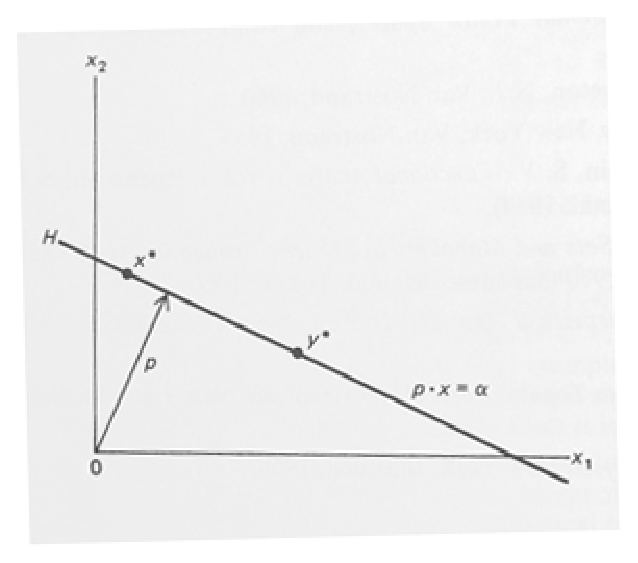
\includegraphics[width=0.47\textwidth]{line}}\hfill
\subfigure[Плоскость]{\includegraphics[width=0.47\textwidth]{3dplane}}
\caption{Примеры гиперплоскостей}\label{fig:Hplanes_exam}
\end{figure}

\begin{note}
Нетрудно проверить, что нормаль всегда ортогональна гиперплоскости.
Действительно, для любых $\vc{x}', \vc{x}'' \in \st{H}$ выполняется

\[\vc{p} \cdot (\vc{x}' - \vc{x}'')= \vc{p} \cdot \vc{x}' - \vc{p}
\cdot \vc{x}''=\gamma - \gamma =0.\]

\noindent В двумерном случае вектор $\vc{p}$ всегда перпендикулярен
прямой (см. Рис.~\ref{fig:Hplanes_exam} а)).
\end{note}

Изменяя значение $\gamma$ (сдвигая гиперплоскость), мы получаем
целое семейство гиперплоскостей. В двумерном случае это выглядит
следующим образом (см. Рис.~\ref{fig:hypermap}).

\input{pics/hypermap.TpX}


\begin{dfn}

\begin{enumerate}
\renewcommand{\theenumi}{(\asbuk{enumi})}

\item Пусть заданы два непустых множества $\st{X}$ и $\st{Y}$ в $\R^n$ и
гиперплоскость $\st{H}= \{ \vc{x}\in \R^n: \vc{p} \cdot \vc{x} =
\gamma\}$. Множества $\st{X}$ и $\st{Y}$ называются
\dw{отделимыми}\index{отделимые множества} гиперплоскостью $\st{H}$,
если $\vc{p} \cdot \vc{x} \leq \gamma$, для всех $\vc{x} \in
\st{X}$, и $\vc{p} \cdot \vc{y} \geq \gamma$, для всех $\vc{y} \in
\st{Y}$.

\item Если указанные неравенства выполняются как строгие ($\vc{p} \cdot \vc{x} < \gamma$
 для всех $\vc{x} \in \st{X}$ и $\vc{p} \cdot \vc{y} > \gamma$ для всех $\vc{y} \in
 \st{Y}$), то множества $\st{X}$ и $\st{Y}$ называют \dw{строго отделимыми}\index{строго отделимые множества}.
\end{enumerate}
\end{dfn}

Гиперплоскость $\st{H}$ в $\R^n$ разбивает $\R^n$ на два
\emph{полупространства} ${\{ \vc{x}: \vc{p} \cdot \vc{x} \leq
\gamma\}}$ и ${\{ \vc{x}: \vc{p} \cdot \vc{x} \geq \gamma\}}$.


\begin{dfn}

Гиперплоскость $\st{H}$ называется \dw{опорной} гиперплоскостью к
множеству $\st{X}$, если эта гиперплоскость имеет общую точку с
$\st{X}$, и множество $\st{X}$ полностью лежит в одном из замкнутых
полупространств, определяемых этой гиперплоскостью.\end{dfn}

Иллюстрация данного определения представлена на Рис.
\ref{fig:sup-hplane}. Здесь гиперплоскость имеет с множеством
$\st{X}$ общую точку $\vc{\hat x}$. В таком случае говорят, что
гиперплоскость является \dw{опорной в точке $\vc{\hat x}$}.

\input{pics/sup_hplane.TpX}

\begin{exer}
Докажите, что:
\begin{itemize}
  \item замкнутое полупространство является выпуклым множеством;
  \item гиперплоскость является замкнутым и выпуклым множеством.
\end{itemize}
\end{exer}

В классической математической экономике те задачи, которые сводятся
к максимизации или минимизации некоторых функций, обычно разрешаются
методами математического анализа. Основной прием, который при этом
используется, -- приравнивание производных нулю -- по существу
эквивалентен отысканию касательной, или опорной, гиперплоскости.
Суть дела здесь не в использовании аналитических методов, а в факте
существования указанных гиперплоскостей, на чем коренным образом
основывается решение многих таких задач.


\begin{teo}(Об отделяющей гиперплоскости, б/д)
\label{teo:sep-hplane}

Пусть $\st{X}$ --- непустое замкнутое выпуклое множество в $\R^n$.
Если точка $\vc{\hat x} \notin \st{X}$, то существует такой вектор
$\vc{p} \in \R^n$, $\vc{p} \neq \vc{0}$, и число $\gamma \in \R$,
что для любого $\vc{x} \in \st{X}$ выполняется:

\[\vc{p} \cdot \vc{x} \leq \gamma < \vc{p} \cdot \vc{\hat x}\]
\end{teo}

Фактически, речь идет о том, что множество  и точка $\vc{\hat x}$
лежат по разные стороны гиперплоскости $\vc{p} \cdot \vc{x} =
\gamma$ (см. Рис.~\ref{fig:sep-hplane} а)). Такая гиперплоскость
называется \dw{отделяющей}.

Тогда, утверждение теоремы можно переформулировать следующим
образом: \emph{для замкнутого выпуклого множества и любой не
принадлежащей ему точки существует отделяющая гиперплоскость}.

\begin{note}

Отметим, что на знаки компонентов вектора $\vc{p}$ ограничения не
накладываются, т.е. для вектора $\vc{p}$ может выполняться как
$\vc{p} \leq \vc{0}$, так и $\vc{p} \geq \vc{0}$, но не $\vc{p} =
\vc{0}$. Аналогично, $\gamma$ может быть больше, меньше, а кроме
того, и равно нулю.
\end{note}


\input{pics/sep_hplane.TpX}

В случае, когда $\vc{\hat x}$ является \emph{граничной} точкой
множества $\st{X}$ (см. Рис.~\ref{fig:sep-hplane} б)), можно
сформулировать следующее утверждение\footnote{См. также
раздел~\vref{app:topology} математического приложения.}.

\begin{teo}(Об опорной гиперплоскости, б/д)

Пусть $\vc{\hat x}$  --- граничная точка замкнутого выпуклого
множества $\st{X}$. Тогда существует опорная к $\st{X}$ в точке
$\vc{\hat x}$ гиперплоскость, т.е. существует такой вектор $\vc{p}
\in \R^n$, $\vc{p} \neq 0$, и число $\gamma \in \R$, что для любого
$x \in \st{X}$ выполняется $\vc{p} \cdot \vc{x} \leq \vc{p} \cdot
\vc{\hat x}$.
\end{teo}

\begin{note}
С другой стороны, это означает, что точка $\vc{\hat x}$ фактически
есть решение задачи:

\[
\left\{ \begin{array}{l}
 \vc{p} \cdot \vc{x} \rightarrow \max\\
 \vc{x} \in \st{X} \\
 \end{array} \right.
\]

Данное соображение понадобится нам ниже при обсуждении эффективных
точек множества.
\end{note}



\begin{teo}\label{teo:sep_hplane_Mink}(Минковского о
разделяющей гиперплоскости, б/д\/\footnote{\cite{Takayama:1985},
\cite{Braverman:1976}})

Пусть $\st{X}$ и $\st{Y}$ -- непустые, необязательно замкнутые,
выпуклые множества в пространстве $\R^n$, не имеющие общих точек
либо имеющие общими только граничные точки, и пусть хотя бы одно из
множеств, например, множество $\st{Y}$, имеет внутреннюю точку (т.е.
$\st{X} \cap \st{Y}^o = \emptyset$).

Тогда существует гиперплоскость, разделяющая эти два множества, т.е.
существует $\vc{p} \in \R^n$, $\vc{p} \neq \vc{0}$, и число $\gamma
\in \R$ такие, что для любого $\vc{x} \in \st{X}$ и любого $\vc{y}
\in \st{Y}$ выполняется соотношение:

\[
\vc{p} \cdot \vc{y} \leq \gamma \leq \vc{p} \cdot \vc{x}.
\]
\end{teo}

\input{pics/sep_sets.TpX}

Заметим, что в этом случае гиперплоскость называется
\dw{разделяющей}.

Утверждение данной теоремы проиллюстрировано на
Рис.~\ref{fig:sep-sets}. В случае \emph{б)} множества $\st{X}$ и
$\st{Y}$ имеют общую граничную точку.

\remrk{Единственность гиперплоскости в случае общей граничной
точки?}

Случай \emph{в)} демонстрирует существенность предположения о том,
что хотя бы одно из множеств должно иметь внутреннюю точку: в этом
случае множества $\st{X}$ и $\st{Y}$ не могут быть разделены.

\begin{exer}
Покажите на примерах, что для невыпуклых множеств это утверждения
трех теорем отделимости не имеют места.
\end{exer}


\begin{teo}(О строгой отделимости, б/д\/\footnote{\cite{Kapustin:2001} стр. 36})

Непустые, непересекающиеся множества $X$ и $Y$, по крайней мере одно
из которых ограничено, строго отделимы. \end{teo}

\section{Лемма Минковского-Фаркаша}

Одним из важнейших приложений теорем об отделимости является лемма
Минковского-Фаркаша, доказательство которой основывается на
соответствующих утверждениях. Однако предварительно мы сформулируем
еще одну лемму.

\begin{lem}

Пусть $\st{K}$ --- конус\index{конус} в пространстве $\R^n$ с
вершиной в нуле и пусть задан вектор $\vc{p} \in \R^n$. Если $\vc{p}
\cdot \vc{x}$ ограничено снизу для любого $\vc{x} \in \st{K}$, то
$\vc{p} \cdot \vc{x} \geq 0$ (для любого $\vc{x} \in \st{K}$).
\end{lem}

\remrk{В приложении дать определение конуса, многогранного выпуклого
конуса.}

\begin{proof}

По предположению об ограниченности $\vc{p} \cdot \vc{x}$, существует
число $\alpha \in \R$ такое, что $\vc{p} \cdot \vc{x} \geq \alpha$
для любого $\vc{x} \in \st{K}$. Поскольку $\st{K}$ является конусом
с вершиной в нуле, тот факт, что $\vc{x} \in \st{K}$ означает, что
$\theta \vc{x} \in \st{K}$ для любого $\theta \geq 0$. Тогда $\vc{p}
\cdot (\theta \vc{x}) \geq \alpha$ или $\vc{p} \cdot \vc{x} \geq
\alpha / \theta$ для любого $\vc{x} \in \st{K}$ и $\theta > 0$.
Рассматривая предел данного соотношения при $\theta \rightarrow
\infty$, получаем $\vc{p} \cdot \vc{x} \geq 0$.
\end{proof}


Сформулируем лемму Минковского-Фаркаша.

\begin{lem}(Минковского-Фаркаша)  \label{lem:MinkFarcas}

Пусть $\vc{a}^1, \vc{a}^2, \ldots, \vc{a}^l$ и $\vc{b}\neq0$ ---
векторы в пространстве $\R^n$. Предположим, что $\vc{b} \cdot \vc{x}
\geq 0$ для любых $\vc{x} \in \R^n$, таких, что $\vc{a}^k \cdot
\vc{x} \geq 0$, $k=1 \ldots l$. Тогда существуют неотрицательные
числа $\lambda_1, \lambda_2, \ldots, \lambda_l$, одновременно не
равные нулю, такие, что $\vc{b}=\sum\limits_{k=1}^l{\lambda_k
\vc{a}^k}$.
\end{lem}

\begin{proof}

Пусть $\st{K}$ --- многогранный выпуклый конус, порожденный
векторами $\vc{a}^1, \vc{a}^2, \ldots, \vc{a}^l$. Тогда $\st{K}$
является замкнутым множеством (\remrk{Почему?}). Необходимо
показать, что $\vc{b} \in \st{K}$.

Предположим, что $\vc{b} \notin \st{K}$. Тогда $\st{K}$ ---
непустое, замкнутое, выпуклое множество, не включающее точку
$\vc{b}$. Тогда, по Теореме \ref{teo:sep-hplane}, существует такой
вектор $\vc{p} \in \R^n$, $\vc{p} \neq 0$, и число $\alpha \in \R$,
что для любого $\vc{x} \in \st{K}$ выполняется\footnote{Знаки
неравенств в утверждении теоремы можно одновременно изменить на
противоположные}:

\[\vc{p} \cdot \vc{x} \geq \alpha > \vc{p} \cdot \vc{b}.\]

Таким образом, $\vc{p} \cdot \vc{x}$ ограничено снизу для любого
$\vc{x} \in \st{K}$. По предыдущей лемме получаем $\vc{p} \cdot
\vc{x} \geq 0$ для любого $\vc{x} \in \st{K}$. Кроме того, поскольку
$\vc{0} \in \st{K}$, $\vc{p} \cdot \vc{0} \geq \alpha$ или $\alpha
\leq 0$. Отсюда $\vc{p} \cdot \vc{b} < 0$.

Поскольку $\vc{a}^k \in \st{K}$, то $\vc{p} \cdot \vc{a}^k \geq 0$,
$k=1 \ldots l$. Тогда для найденного вектора $\vc{p}$ получаем
$\vc{b} \cdot \vc{p} < 0$ при $\vc{p} \cdot \vc{a}^k \geq 0$, $k=1
\ldots l$. Это противоречит условию теоремы. Значит, $\vc{b} \in
\st{K}$. По свойству многогранного выпуклого конуса, это означает,
что существуют неотрицательные числа $\lambda_1, \lambda_2, \ldots,
\lambda_l$, такие, что $\vc{b}=\sum\limits_{k=1}^l{\lambda_k
\vc{a}^k}$. Поскольку $\vc{b}\neq0$, числа $\lambda_1, \lambda_2,
\ldots, \lambda_l$ не могут быть одновременно равны нулю.


\end{proof}


\begin{note}(к лемме Минковского-Фаркаша)

\begin{enumerate}
\renewcommand{\theenumi}{(\alph{enumi})}

  \item Если $b=0$, то допускается одновременное равенство нулю всех
  $\lambda_k$, $k=1 \ldots l$.

  \item Верно и обратное утверждение относительно Леммы \ref{lem:MinkFarcas},
  а именно, если $\vc{a}^1, \vc{a}^2, \ldots, \vc{a}^l$ и $\vc{b}\neq0$
  ---  векторы в пространстве $\R^n$ и существуют неотрицательные
   коэффициенты $\lambda_1, \lambda_2, \ldots, \lambda_l$,
   одновременно не равные нулю, такие, что $\vc{b}=\sum\limits_{k=1}^l{\lambda_k
   \vc{a}^k}$,то $\vc{b} \cdot \vc{x} \geq 0$ для любых $\vc{x} \in \R^n$, таких,
   что $\vc{a}^k \cdot \vc{x} \geq 0$, $k=1 \ldots l$.

\end{enumerate}

\end{note}


\remrk{Можно добавить векторно-матричную и геометрическую
интерпре\-тацию леммы из \cite{Takayama:1985}, стр. 47.}

Лемма Минковского-Фаркаша играет важную роль в теории линейного
программирования, теории игр, теории нелинейного программирования и
т.д.

\newpage

\section{Эффективные точки на выпуклых
множествах\protect\footnote{\cite{Takayama:1985}}}

Особую роль в экономическом анализе играют эффективные точки
различных множеств. Можно ввести следующие определения.

\begin{dfn}

Пусть $\st{X} \subset \R^n$ --- некоторое замкнутое множество.

\begin{enumerate}
  \item Точка ${\vc{\hat x}} \in \st{X} $ называется (\textbf{строго}) \textbf{эффективной
точкой} этого множества, если не существует другой точки $\vc{x} \in
\st{X}$, такой, что $\vc{x} \geq \vc{\hat x}$.

  \item Точка $\vc{\tilde x} \in \st{X}$ называется \textbf{слабо эффективной} точкой
множества~$\st{X}$, если не существует другой точки $\vc{x} \in
\st{X}$, такой, что $\vc{x} \gg \vc{\tilde x}$.

\end{enumerate}
\end{dfn}

Из приведенного выше определения нетрудно видеть, что любая
эффективная точка является и слабо эффективной. С другой стороны,
если точка не является слабо эффективной, то она не может быть и
строго эффективной.

\begin{comm}
Проиллюстрируем идею эффективной точки множества на простом примере.
Классический пример выпуклого множества, приводимый в элементарных
учебниках по экономической теории --- множество производственных
возможностей страны, ограниченное \dw{кривой производственных
возможностей} (англ., \emph{production possibility
frontier}\footnote{\cite{McConnell:1996}}). Кривая производственных
возможностей представлена на Рис.~\ref{fig:ppfrontier}.

Стандартно предполагается, что при ограниченных запасах факторов
производства, в экономике производятся два вида товаров: пушки и
масло. Все сочетания пушек и масла на кривой производственных
возможностей представляют максимальные их количества, которые могут
быть получены лишь в результате наиболее эффективного использования
всех имеющихся ресурсов.

Чтобы осуществить производство различных комбинаций пушек и масла,
представленных на графике, общество должно обеспечить полную
занятость ресурсов и полный объем производства. Таким образом,
каждая точка на кривой производственных возможностей представляет
собой какой-то максимальный объем производства двух указанных
товаров.

\input{pics/ppfrontier.TpX}

Эффективная точка есть граничная точка множества производственных
возможностей $\st{X}$. Действительно, как видно на
Рис.~\ref{fig:ppfrontier} \emph{а)}, точка $\vc{\hat x}$ является
\emph{эффективной}, поскольку все точки $\vc{x}$, такие, что $\vc{x}
\geq \vc{\hat x}$ (т.\/е. точки, находящиеся выше и правее $\vc{\hat
x}$), не принадлежат множеству $\st{X}$. По аналогичным соображениям
точка $\vc{\bar x}$ эффективной не является.

Следует отметить, что эффективная точка множества производственных
возможностей представляет собой такую комбинацию затрат-выпуска, что
невозможно увеличить выпуск по одного из товаров, не уменьшив
выпуска другого товара или не увеличив расход ресурсов.

На Рис.~\ref{fig:ppfrontier} \emph{б)} приведен пример \emph{слабо
эффективной} точки. Если предположить, что кривая производственных
возможностей страны имеет линейные горизонтальный и вертикальный
участки ($AB$ и $CD$ соответственно), как показано на рисунке, то
точки, лежащие на этих участках, являются слабо эффективными.

Действительно, точка $\vc{\tilde x}$ является слабо эффективной,
поскольку не существует другой точки $\vc{x}$, лежащей в множестве
$\st{X}$, такой, что $\vc{x} \gg \vc{\tilde x}$.

\end{comm}


Сформулируем следующие фундаментальные теоремы.

\begin{teop}(Условия эффективности точки)\label{teo:1_fund_production}

Пусть $\st{X} \subset \R^n$ --- некоторое (замкнутое) множество.
Пусть $\vc{\hat x}$ есть решение задачи:

\begin{equation}\label{eq:eff_conditions}
\left\{ \begin{array}{l}
 \vc{p} \cdot \vc{x} = p_1x_1 + \ldots + p_n x_n\to \max  \\
 \vc{x} \in \st{X} \\
 \end{array} \right.
\end{equation}


\begin{enumerate}
\renewcommand{\theenumi}{(\roman{enumi})}
  \item Если $\vc{p} \geq \vc{0}$, то точка $\vc{\hat x} \in \st{X}$ является
  слабо эффективной.
  \item Если $\vc{p} \gg \vc{0}$, то точка $\vc{\hat x} \in \st{X}$ является
  эффективной.
\end{enumerate}

\end{teop}

\begin{proof}(От противного)

(i) Предположим, что утверждение данного пункта не выполняется. В
этом случае существует $\vc{\bar x} \in \st{X}$ такой, что $\vc{\bar
x} \gg \vc{\hat x}$. Тогда, поскольку $\vc{p} \geq \vc{0}$, получаем
$\vc{p} \cdot \vc{\bar x} > \vc{p} \cdot \vc{\hat x}$. Однако это
противоречит тому факту, что $\vc{\hat x}$ есть решение задачи
(\ref{eq:eff_conditions}).

(ii) Докажите самостоятельно в качестве \textbf{упражнения}.

\end{proof}



Отметим, что в приведенных теоремах не накладывается никаких условий
на множество $\st{X}$. Обратное утверждение требует более сильных
предположений относительно устройства множества $\st{X}$, а именно,
выпуклости этого множества. Для доказательства обратного утверждения
потребуется следующая лемма.

\begin{lem}

Пусть $\st{X} \subset \R^n$ --- некоторое замкнутое множество. Если
$\vc{\hat x}$ является слабо эффективной точкой множества $\st{X}$,
то $\st{X} \cap \st{Z}^o=\emptyset$, где $\st{Z}^o=\{\vc{z} \in
\R^n: \vc{z} \gg \vc{\hat x}\}$.\end{lem}

\begin{proof}(От противного)

Предположим, что утверждение леммы не выполняется. Тогда существует
$\vc{z} \in \st{X}$ такой, что $\vc{z} \gg \vc{\hat x}$. Тогда
$\vc{\hat x}$ не является (слабо) эффективной точкой множества
$\st{X}$, что противоречит предположению леммы.

\end{proof}

\begin{exer}
Докажите, что если  $\vc{\hat x}$ является строго эффективной точкой
множества $\st{X}$, то $\st{X} \cap \st{Z}=\{\vc{\hat x}\}$, где
$\st{Z}=\{\vc{z}\in \R^n: \vc{z} \geqq \vc{\hat x}\}$.
\end{exer}

\begin{exer}
Докажите, что в обоих случаях множество $\st{Z}$ является выпуклым.
\end{exer}

\begin{teop}(Свойство слабо эффективной точки)\label{teo:2_fund_production}

Пусть $\st{X} \subset \R^n$ --- выпуклое и замкнутое множество. Если
точка ${\vc{\hat x} \in \st{X}}$ является слабо эффективной точкой
множества $\st{X}$, то существует вектор ${\vc{p} \geq \vc{0}}$,
$\vc{p} \in \R^n$, такой, что $\vc{p} \cdot \vc{\hat x} \geq \vc{p}
\cdot \vc{x}$ для любых $\vc{x} \in \st{X}$, т.е. $\vc{\hat x}$ есть
решение задачи (\ref{eq:eff_conditions}).
\end{teop}

\begin{proof}

Пусть $\st{Z}=\{\vc{z}\in \R^n: \vc{z} \geqq \vc{\hat x}\}$.

Тогда $\st{Z}^o=\{\vc{z} \in \R^n: \vc{z} \gg \vc{\hat x}\} \neq
\emptyset$. Множество $\st{Z}^o$ является выпуклым. Поскольку
$\vc{\hat x}$ является слабо эффективной точкой множества $\st{X}$,
то, по предыдущей лемме, $\st{X} \cap \st{Z}^o=\emptyset$. Таким
образом, имеем два непересекающихся множества, внутренность по
крайней мере одного из которых непуста.

Значит, по теореме отделимости Минковского
(Теорема~\ref{teo:sep_hplane_Mink}), найдутся $\vc{p} \in \R^n$,
$\vc{p}\neq \vc{0}$, и число $\gamma \in \R$ такие, что для любого
$\vc{x} \in \st{X}$ и любого $\vc{z} \in \st{Z}^o$ выполняется
соотношение:

\[
\vc{p} \cdot \vc{x} \leq \gamma \leq \vc{p} \cdot \vc{z}.
\]

Отметим, что $\gamma = \vc{p} \cdot \vc{\hat x}$. Действительно,
поскольку $\vc{\hat x} \in \st{X}$, то $\gamma \geq \vc{p} \cdot
\vc{\hat x}$. С другой стороны, $\gamma \leq \vc{p} \cdot \vc{\hat
x}$. Действительно, если это не так, то $\vc{p} \cdot \vc{z}\geq
\gamma> \vc{p} \cdot \vc{\hat x}$ должно выполняться для любого
$\vc{z} \in \st{Z}^o$. Однако, это невозможно: мы всегда можем
подобрать такое $\vc{\bar z}$, что $\vc{p}\cdot\vc{\bar z}<\gamma$.
Отсюда следует, что $\gamma = \vc{p} \cdot \vc{\hat x}$.

Кроме того, $\vc{p} \geq \vc{0}$ (если это не так, то найдется такая
компонента ${p_i < 0}$ вектора $\vc{p}$, что, подобрав достаточно
большую по значению компоненту $z_i$ вектора $\vc{z}$, мы получим
$\vc{p} \cdot \vc{z}<\vc{p} \cdot \vc{\hat x}$, что является
противоречием).

Таким образом, мы получили, что для любого $\vc{x} \in \st{X}$
выполняется $\vc{p} \cdot \vc{x} \leq \vc{p} \cdot \vc{\hat x}$,
причем $\vc{p} \geq \vc{0}$.
\end{proof}

\begin{note}
\begin{enumerate}
  \item Если множество $\st{X}$ является многогранным выпуклым конусом, то в
условиях сформулированной выше теоремы можно показать, что $\vc{p}
\gg \vc{0}$. Вообще говоря, только в этом случае можно утверждать,
что точка $\vc{\hat x}$ является строго эффективной.

  \item Напомним, что всякая строго эффективная точка
  является и слабо эффективной. В общем же случае нельзя сформулировать
  условия подобного рода для строгой эффективности точки.

  Действительно, из того факта, что точка
  является эффективной, вовсе не следует, что $\vc{p} \gg \vc{0}$. В
  качестве примера на Рис.~\ref{fig:circle_eff} приведем окружность (выпуклое
  множество), точка $A$ которой очевидным образом является
  эффективной, но $\vc{p} \geq \vc{0}$. (В качестве \textbf{упражнения}
  аккуратно докажите этот факт).

\input{pics/circle_eff.TpX}

\end{enumerate}


\end{note}


\begin{comm}

Теоремы ~\ref{teo:1_fund_production} и \ref{teo:2_fund_production}
позволяют описать идею эффективной точки множества с точки зрения
задачи максимизации, а именно, с учетом доказанного в теореме
утверждения, можно говорить о том, что любая эффективная точка
множества $\st{X}$ есть, при некотором $\vc{p} \geq \vc{0}$, решение
следующей задачи:

\[
\left\{ \begin{array}{l}
 \vc{p} \cdot \vc{x} \to \max  \\
 \vc{x} \in \st{X} \\
 \end{array} \right.
\]

Данное соображение поддается прозрачной экономической интерпретации.
Если в рассматриваемом нами примере про кривую производственных
возможностей страны точка $\vc{\hat x}$ является эффективной, и
страна \emph{фактически} производит указанный набор товаров
$\vc{\hat x}=(\hat x_1, \hat x_2)$, то можно утверждать, что в
данной точке национальный доход:

\[
I = \vc{p} \cdot \vc{\hat x}= p_1\hat x_1 + p_2 \hat x_2
\]

\noindent достигает своего максимума. При этом, вектор $\vc{p} \geq
\vc{0}$ трактуется как вектор цен на соответствующие товары.

Иллюстрация данной идеи представлена на Рис.~\ref{fig:ppfront_max}.

\input{pics/ppfront_max.TpX}

\end{comm}


\newpage

\section{Оптимальность по
Парето\protect\footnote{[Конспект ЕУ по математике]}}

Рассмотрим $\st{X} \subset \R^n$ и набор функций $f_1(\vc{x}),
f_2(\vc{x}), \ldots, f_m(\vc{x})$.

\begin{dfn}(Доминирование по Парето)

\begin{enumerate}
\item Будем говорить, что точка $\vc{\tilde x} \in \st{X}$ \dw{доминирует} точку
$\vc{\hat x} \in \st{X}$ \dw{по Парето}, если $f_j(\vc{\tilde x})
\geq f_j(\vc{\hat x})$, $j=1 \ldots m$, и хотя бы одно из этих
неравенств выполняется, как строгое.

\item Будем говорить, что точка $\vc{\tilde x}$ \dw{строго доминирует} точку
$\vc{\hat x}$ \dw{по Парето}, если $f_j(\vc{\tilde x}) >
f_j(\vc{\hat x})$, $j=1 \ldots m$.
\end{enumerate}
\end{dfn}

\begin{dfn}(Оптимальность по Парето)

\begin{enumerate}

\item Будем говорить, что точка $\vc{\hat x} \in \st{X}$ является \dw{оптимальной
по Парето}, если $\nexists \,{\vc{\tilde x}} \in \st{X}$, такой, что
точка $\vc{\tilde x}$ доминирует точку $\vc{\hat x}$ по Парето.

\item Будем говорить, что точка $\vc{\hat x} \in \st{X}$ является \dw{слабо
оптимальной по Парето}, если $\nexists \,{\vc{\tilde x}} \in
\st{X}$, такой, что точка $\vc{\tilde x}$ строго доминирует точку
$\vc{\hat x}$ по Парето.

\end{enumerate}
\end{dfn}

Сформулируем следующие важные теоремы.

\begin{teop}\label{teo:Pareto_opt_conditions}(Условия оптимальности точки)

Пусть $\st{X}$ --- замкнутое множество, и $\vc{\hat x} \in \st{X}$
есть решение задачи:

\[ \left\{
\begin{array}{l}
 p_1 f_1 (\vc{x}) + p_2 f_2 (\vc{x}) + \ldots + p_m f_m (\vc{x})\to \max  \\
 \vc{x} \in \st{X} \\
 \end{array} \right.
\]

\begin{enumerate}
\renewcommand{\theenumi}{(\roman{enumi})}

\item Если коэффициенты $p_j$, $j=1 \ldots m$, неотрицательны и одновременно не равны нулю,
т.е. $\vc{p} \geq \vc{0}$, то $\vc{\hat x}$ будет слабо оптимальной
по Парето точкой.

\item Если $p_j > 0$, $j=1 \ldots m$, т.е. $\vc{p} \gg \vc{0}$, то $\vc{\hat x}$ ---
оптимальная по Парето точка.

\end{enumerate}
\end{teop}

\begin{proof}
Доказательство данной теоремы выполните в качестве
\textbf{упражнения}.
\end{proof}

Для доказательства следующей теоремы нам потребуется следующая
Фундаментальная лемма.


\begin{lemp}(Фундаментальная лемма)

Пусть $\st{X}$ --- выпуклое замкнутое множество, а заданные на нем
функции $f_1(\vc{x}), f_2(\vc{x}), \ldots, f_m(\vc{x})$ --- вогнуты
($f_j: \st{X} \rightarrow \R$, $j=1 \ldots m$). Пусть числа $b_1,
b_2, \ldots, b_m$ таковы, что система неравенств

\[
\left\{ \begin{array}{l}
 f_1(\vc{x}) > b_1\\
 f_2(\vc{x}) > b_2 \\
  \cdots  \\
 f_m(\vc{x}) > b_m \\
 \end{array} \right.
\]

\noindent не имеет решения ни для какого $\vc{x} \in \st{X}$.

Тогда существуют такие неотрицательные коэффициенты $p_1, p_2,
\ldots, p_m$, не все одновременно равные нулю, что для любого
$\vc{x} \in \st{X}$ выполняется соотношение:

\begin{equation}\label{eq:ineq_fund_lemma}
p_1 f_1(\vc{x}) + p_2 f_2(\vc{x}) + \ldots + p_m f_m(\vc{x}) \leq
p_1 b_1 + p_2 b_2 + \ldots + p_m b_m.
\end{equation}

\end{lemp}

\remrk{Связь с Фаркашем?}

\begin{proof}

Для каждой точки $\vc{x} \in \st{X}$ определим множество
${\st{Z}_{\vc{x}} \subset \R^m}$ следующим образом:

\[
\st{Z}_{\vc{x}}=\{\vc{z}\in \R^m: z_1\leq f_1(\vc{x}), z_2\leq
f_2(\vc{x}), \ldots, z_m\leq f_m(\vc{x})\}.
\]

Обозначим $\st{Z}= \mathop \cup \limits_{\vc{x} \in \st{X}}
\st{Z}_{\vc{x}}$.

Отметим, что множество $\st{Z}$ является выпуклым. Действительно,
возьмем точки $\vc{z'} \in \st{Z}_{\vc{x'}}$ и $\vc{z''} \in
\st{Z}_{\vc{x''}}$ (очевидно, что $\vc{z'}, \vc{z''} \in \st{Z}$) и
число $\theta \in \R$, $0 \leq \theta \leq 1$. Тогда для всех $j=1
\ldots m$ выполняется:

\[
\bar{z}_{j}= \theta z'_j + (1- \theta) z''_j\leq  \theta
f_j(\vc{x'}) + (1- \theta) f_j(\vc{x''}) \leq  f_j(\theta\vc{x'} +
(1- \theta) \vc{x''})=f_j(\vc{\bar x}),
\]

\noindent где $\vc{\bar x}=\theta\vc{x'} + (1- \theta) \vc{x''} \in
\st{X}$, а последнее неравенство справедливо в силу вогнутости
функций $f_j$. Тогда

\[
\vc{\bar z} = \left( {\begin{array}{*{20}c}
   \bar{z}_1  \\
   \bar{z}_2  \\
    \vdots   \\
   \bar{z}_m  \\
\end{array}} \right) \in \st{Z}_{\vc{\bar x}} \subset \st{Z},
\]

\noindent что доказывает выпуклость множества $\st{Z}$.

Далее, отметим, что точка $\vc{b} =(b_1, b_2, \ldots, b_m)\notin
\st{Z}$. Действительно, если бы $\vc{b} \in \st{Z}$, то нашелся бы
такой вектор $\vc{\tilde x} \in \st{X}$, что $\vc{b} \in
\st{Z}_{\vc{\tilde x}}$, а значит, $f_j(\vc{\tilde x}) \geq b_j$ для
всех $j=1 \ldots m$, что противоречит условию леммы.

Тогда, по Теореме~\ref{teo:sep-hplane}, множество $\st{Z}$ и точка
$\vc{b}$ отделимы, т.\,е. существует такой вектор $\vc{p} \in \R^m$,
$\vc{p} \neq \vc{0}$, что для любого $\vc{z} \in \st{Z}$

\begin{equation}\label{eq:ineq1_fundlemma}
\vc{p} \cdot \vc{z} \leq \vc{p} \cdot \vc{b}.
\end{equation}

Преобразуя данное неравенство, получаем:

\begin{equation}\label{eq:ineq2_fundlemma}
\vc{p} \cdot (\vc{z} - \vc{b}) \leq 0.
\end{equation}


Поскольку, очевидно, $\vc{z} \leq \vc{b}$ для любого $\vc{z} \in
\st{Z}$, то любая из компонент вектора $(\vc{z} - \vc{b})$ может
принимать сколь угодно большие отрицательные значения. Это в свою
очередь означает, что, для выполнения
неравенства~(\ref{eq:ineq2_fundlemma}), все компоненты вектора
$\vc{p}$ должны быть неотрицательны.

Раскрывая неравенство~(\ref{eq:ineq1_fundlemma}) с учетом
определения множества $\st{Z}_{\vc{x}}$, получаем, что для любого
$\vc{x}\in \st{X}$ существует такой вектор $\vc{p}\geq \vc{0}$, что

\begin{multline}
p_1 z_1 + p_2 z_2 + \ldots + p_m z_m \leq p_1 f_1(\vc{x}) + p_2
f_2(\vc{x}) + \ldots + p_m f_m(\vc{x}) \leq {}\\ \leq p_1 b_1 + p_2
b_2 + \ldots + p_m b_m.
\end{multline}


Последняя часть полученного неравенства доказывает утверждение
леммы.

\end{proof}

Теперь мы можем приступить к доказательству следующего важного
свойства слабо оптимальной точки.

\begin{teop}(Свойство слабо оптимальной
по Парето точки)

Пусть $\st{X}$ --- замкнутое выпуклое множество в $\R^n$. Пусть
заданы вогнутые функции $f_1(\vc{x}), f_2(\vc{x}), \ldots,
f_m(\vc{x}): \st{X} \to \R$.

Если $\vc{\hat x} \in \st{X}$ является слабо оптимальной по Парето
точкой, то существуют неотрицательные коэффициенты $p_1, p_2,
\ldots, p_m$, не все одновременно равные нулю, такие, что $\vc{\hat
x}$ представляет собой решение задачи:

\[ \left\{
\begin{array}{l}
 p_1 f_1(\vc{x}) + p_2 f_2(\vc{x}) + \ldots + p_m f_m(\vc{x})\to \max  \\
 \vc{x} \in \st{X} \\
 \end{array} \right.
\]
\end{teop}

\begin{proof}

Обозначим
\begin{align*}
 b_1 &=f_1(\vc{\hat x}),\\
 b_2 &=f_2(\vc{\hat x}),\\
  &\cdots \\
 b_m &=f_m(\vc{\hat x}).
\end{align*}

Поскольку $\vc{\hat x}$ является слабо оптимальной по Парето точкой,
это означает, что $\nexists \, \vc{\tilde x} \in \st{X}:
f_j(\vc{\tilde x})> f_j(\vc{\hat x})$, $j=1 \ldots m$.

Другими словами, с учетом введенных обозначений, система неравенств

\[
\left\{ \begin{array}{l}
 f_1(\vc{x}) > b_1\\
 f_2(\vc{x}) > b_2 \\
  \cdots  \\
 f_m(\vc{x}) > b_m \\
 \end{array} \right.
\]

\noindent не имеет решения ни при каком $\vc{x} \in \st{X}$.

Тогда, в соответствии с утверждением доказанной выше Фундаментальной
леммы, существуют неотрицательные коэффициенты $p_1, p_2, \ldots,
p_m$, не все одновременно равные нулю, такие, что для любого $\vc{x}
\in \st{X}$ выполняется соотношение:

\begin{multline}
p_1 f_1(\vc{x}) + p_2 f_2(\vc{x}) + \ldots + p_m f_m(\vc{x}) \leq
p_1 b_1 + p_2 b_2 + \ldots + p_m b_m = \\ = p_1 f_1(\vc{\hat x}) +
p_2 f_2(\vc{\hat x}) + \ldots + p_m f_m(\vc{\hat x}).
\end{multline}

\noindent  Отсюда получаем, что
\[p_1 f_1(\vc{x}) + p_2 f_2(\vc{x}) + \ldots + p_m
f_m(\vc{x}) \leq p_1 f_1(\vc{\hat x}) + p_2 f_2(\vc{\hat x}) +
\ldots + p_m f_m(\vc{\hat x}). \]

\noindent Это означает, что точка $\vc{\hat x}$ представляет собой
решение задачи:

\[ \left\{
\begin{array}{l}
 p_1 f_1(\vc{x}) + p_2 f_2(\vc{x}) + \ldots + p_m f_m(\vc{x})\to \max  \\
 \vc{x} \in \st{X} \\
 \end{array} \right.
\]


\end{proof}



\section{Общая теорема Куна-Таккера}

\begin{dfn}
Задача максимизации вогнутой функции на выпуклом (замкнутом?)
множестве называется \dw{задачей выпуклого программирования}.
\end{dfn}

Формально, задачу выпуклого программирования можно записать
следующим образом:

\begin{equation}\label{problem:ZVPG}
\left\{ \begin{array}{l}
 f_0(\vc{x}) \to \max  \\
 \vc{x} \in \st{G} \\
 \end{array} \right.
\end{equation}

\noindent где $\st{G}=\{\vc{x} \in \st{X}:  f_j (\vc{x}) \geq b_j, j
= 1 \ldots m \}$, $\st{X}$ --- выпуклое и замкнутое множество, а
функции $f_0(\vc{x}), f_1(\vc{x}), \ldots, f_m(\vc{x})$ ---
вогнутые.

\begin{exer}
Покажите, что множество $\st{G}$ является выпуклым и замкнутым.
\end{exer}

Отметим, что если $\st{X}\equiv \R^n$, то
задача~(\ref{problem:ZVPG}) называется \dw{основной (общей) задачей
выпуклого программирования}. Для удобства
задачу~(\ref{problem:ZVPG}) часто записывают в виде:

\begin{equation}\label{problem:ZVP}
\left\{ \begin{array}{l}
 f_0(\vc{x}) \to \max  \\
 f_j (\vc{x}) \geq b_j, j = 1 \ldots m\\
 \vc{x} \in \st{X} \\
 \end{array} \right.
\end{equation}

Часто в литературе ограничения на функции $f_j(\vc{x})$ записывают в
виде $f_j (\vc{x}) \geq 0$. Отметим, что постановка
задачи~(\ref{problem:ZVP}) не противоречит данному подходу.
Действительно, перенося $b_j$ в левые части ограничений-неравенств,
получаем, $g_j (\vc{x})=f_j (\vc{x}) - b_j\geq 0$, где функции $g_j
(\vc{x})$ по-прежнему являются вогнутыми, поскольку вычитание или
прибавление константы к вогнутой функции не влияет на ее вогнутость.
Здесь и далее мы будем придерживаться обозначений, введенных для
задачи~(\ref{problem:ZVP}).

Продолжая тему оптимальности по Парето из предыдущего раздела,
отметим следующий важный факт.

\begin{prop}\label{prop:x_weakoptimal}
Если $\vc{\hat x}$ есть решение задачи~(\ref{problem:ZVP}), то
$\vc{\hat x}$ --- слабо оптимальная по Парето точка относительно
набора функций $f_0, f_1, \ldots, f_m$.
\end{prop}

\begin{proof}(От противного)

Пусть $\vc{\hat x}$ не является слабо оптимальной по Парето точкой.
Тогда $\exists \,\vc{\tilde x} \in \st{X}$, такая, что

\[
\left\{ \begin{array}{l}
 f_0(\vc{\tilde x}) > f_0(\vc{\hat x})\\
 f_1(\vc{\tilde x}) > f_1(\vc{\hat x})\\
  \cdots  \\
 f_m(\vc{\tilde x}) > f_m(\vc{\hat x}) \\
 \end{array} \right.
\]

\noindent Таким образом, с одной стороны $\vc{\tilde x}\in \st{X}$
удовлетворяет ограничениям задачи ($f_j(\vc{\tilde x}) >
f_j(\vc{\hat x})\geq b_j$, $j=1 \ldots m$), а с другой стороны,
${f_0(\vc{\tilde x}) > f_0(\vc{\hat x})}$. Это означает, что
$\vc{\hat x}$ не является решением задачи~(\ref{problem:ZVP}).
Получили противоречие. Значит, $\vc{\hat x}$ является слабо
оптимальной по Парето точкой.
\end{proof}



\begin{exer}
Укажите, при каких условиях решение задачи~(\ref{problem:ZVP}) есть
строго оптимальная по Парето точка.
\end{exer}


\subsection{Понятие условий регулярности}

В утверждениях данного раздела нам понадобится ввести некоторые
предположения об устройстве множества $\st{X}$ --- так называемые
\dw{условия регулярности} множества.

\begin{dfn}(Обычная регулярность, Карманов, стр. 50)

Если для любого $j=1 \ldots m$ существует такая точка $\vc{x}_j \in
\st{X}$, что

\[
 f_j(\vc{x}_j) > b_j,\\
\]

\noindent то говорят, что множество $\st{X}$ удовлетворяет условию
регулярности.

\end{dfn}



\begin{dfn}(Регулярность по Слейтеру)

Если в множестве $\st{X}$ существует такой вектор $\vc{\bar x}$, для
которого при произвольных $b_1, \ldots, b_m$ выполняется:

\[
\left\{ \begin{array}{l}
 f_1(\vc{\bar x}) > b_1\\
 f_2(\vc{\bar x}) > b_2 \\
  \cdots  \\
 f_m(\vc{\bar x}) > b_m \\
 \end{array} \right.
\]

\noindent то говорят, что множество $\st{X}$ \dw{регулярно по
Слейтеру} (или для него выполняется \dw{условие Слейтера}).

\end{dfn}

\begin{dfn} (Регулярность по Карлину)

Множество $\st{X}$ является \dw{регулярным по Карлину}, если для
любого вектора $\vc{p} \geq \vc{0}$ и произвольных $b_1, \ldots,
b_m$ существует такой вектор $\vc{\bar x} \in \st{X}$, что:
\[
p_1 f_1(\vc{\bar x}) + p_2 f_2(\vc{\bar x}) + \ldots + p_m
f_m(\vc{\bar x}) > p_1 b_1 + p_2 b_2 + \ldots + p_m b_m.
\]

\end{dfn}

\begin{exer}
Проверьте, что все три условия регулярности эквивалентны.
\end{exer}


\subsection{Предварительные предложения}

Сформулируем следующее предложение.

\begin{prop}\label{prop:necessity_TKT}

Пусть $\st{X}$ --- выпуклое множество в $\R^n$. Пусть заданы
вогнутые функции $f_0, f_1, f_2, \ldots, f_m: \st{X} \to \R$. Пусть
$\vc{\hat x}$ есть решение задачи~(\ref{problem:ZVP}).

Тогда существуют неотрицательные коэффициенты $p_0, p_1, \ldots,
p_m$, не все одновременно равные нулю, такие, что $\vc{\hat x}$ есть
решение задачи:

\[
\left\{ \begin{array}{l}
 p_0 f_0(\vc{x}) + p_1 f_1(\vc{x})+ \ldots + p_m f_m(\vc{x}) \to \max  \\
 \vc{x} \in \st{X} \\
 \end{array} \right.
\]

\end{prop}

\begin{proof}
Доказательство этого утверждения мгновенно вытекает из свойства
слабо оптимальной по Парето точки.

Действительно, поскольку $\vc{\hat x}$ есть решение
задачи~(\ref{problem:ZVP}), то, по
Предложению~\ref{prop:x_weakoptimal}, $\vc{\hat x}$ является слабо
оптимальной по Парето точкой. Тогда, по свойству слабо оптимальной
точки (Теорема~\ref{teo:property_weak_optimal}), найдутся
неотрицательные коэффициенты $p_0, p_1, p_2, \ldots, p_m$, не все
одновременно равные нулю, такие, что $\vc{\hat x}$ есть решение
задачи:

\[
\left\{ \begin{array}{l}
 p_0 f_0(\vc{x}) + p_1 f_1(\vc{x})+ \ldots + p_m f_m(\vc{x}) \to \max  \\
 \vc{x} \in \st{X} \\
 \end{array} \right.
\]

\end{proof}

Отметим, что сформулированное выше утверждение верно и в обратную
сторону. Однако, при этом, не требуется выпуклость множества
$\st{X}$.

\begin{prop}\label{prop:sufficiency_TKT}

Пусть заданы вогнутые функции $f_0, f_1, f_2, \ldots, f_m: \st{X}
\to \R$. Пусть ${\vc{\hat x} \in \st{X}}$ есть решение задачи:

\[
\left\{ \begin{array}{l}
 f_0(\vc{x}) + p_1 f_1(\vc{x})+ \ldots + p_m f_m(\vc{x}) \to \max  \\
 \vc{x} \in \st{X} \\
 \end{array} \right.
\]

\noindent где $p_1,p_2 \ldots, p_m$ --- неотрицательные
коэффициенты, не все одновременно равные нулю.

Тогда $\vc{\hat x}$ есть решение задачи~(\ref{problem:ZVP}) для
некоторых (каких?) $b_1, b_2, \ldots, b_m$.

\end{prop}

\begin{proof}
Доказательство данного утверждения вытекает из условия оптимальности
по Парето (Теорема~\ref{teo:Pareto_opt_conditions}). Действительно,
положив $p_0=1$, заметим, что $\vc{\hat x}$ есть решение задачи:

\[
\left\{ \begin{array}{l}
 p_0 f_0(\vc{x}) + p_1 f_1(\vc{x})+ \ldots + p_m f_m(\vc{x}) \to \max  \\
 \vc{x} \in \st{X}, \\
 \end{array} \right.
\]

\noindent где $p_0, p_1, p_2 \ldots, p_m$ --- неотрицательные
коэффициенты, не все одновременно равные нулю. Тогда, по
Теореме~\ref{teo:Pareto_opt_conditions}, $\vc{\hat x}$ есть слабо
оптимальная по Парето точка, т.е. $\nexists\, \vc{\tilde x} \in
\st{X}$ такого, что:

\[
\left\{ \begin{array}{l}
 f_0(\vc{\tilde x}) > f_0(\vc{\hat x})\\
 f_1(\vc{\tilde x}) > f_1(\vc{\hat x})\\
  \cdots  \\
 f_m(\vc{\tilde x}) > f_m(\vc{\hat x}) \\
 \end{array} \right.
\]

Выбрав $b_1=f_1(\vc{\hat x})$, $b_2=f_2(\vc{\hat x}), \ldots$,
$b_m=f_m(\vc{\hat x})$, получаем, что не существует точки
$\vc{\tilde x} \in \st{X}$, которая, с одной стороны, удовлетворяла
бы системе ограничений задачи~(\ref{problem:ZVP}), и для которой, с
другой стороны, выполнялось бы $f_0(\vc{\tilde x}) > f_0(\vc{\hat
x})$.

Это означает, что точка $\vc{\hat x}$ есть решение
задачи~(\ref{problem:ZVP}).

\end{proof}


\subsection{Основная теорема Куна-Таккера}


Сформулируем основную теорему Куна-Таккера.

\begin{teop}(Теорема Куна-Таккера-Узавы)

Пусть $\st{X}$ --- выпуклое множество в $\R^n$. Пусть заданы
вогнутые функции $f_0, f_1, f_2, \ldots, f_m: \st{X} \to \R$. Пусть
выполнено условие Слейтера (т.е. $\exists \, \vc{\bar x} \in
\st{X}:$ ${f_j(\vc{\bar x}) > b_j}$, ${j=1 \ldots m}$).

Точка $\vc{\hat x}\in \st{X}$ есть решение
задачи~(\ref{problem:ZVP}) тогда и только тогда, когда существуют
неотрицательные коэффициенты $\hat p_1, \hat p_2 \ldots, \hat p_m$,
не все одновременно равные нулю, такие, что:

\begin{enumerate}
\renewcommand{\theenumi}{(\arabic{enumi})}
\item точка $\vc{\hat x}$ есть решение задачи:

\[
\left\{ \begin{array}{l}
 f_0(\vc{x}) + \hat p_1 f_1(\vc{x})+ \ldots + \hat p_m f_m(\vc{x}) \to \max  \\
 \vc{x} \in \st{X} \\
 \end{array} \right.
\]


\item выполняются условия \dw{дополняющей нежесткости}:
\[f_j(\vc{\hat x}) > b_j \Rightarrow \hat p_j =0.\]

\end{enumerate}
\end{teop}

Условие дополняющей нежесткости фактически означает, что если на
оптимальном плане некоторое $j$-е неравенство выполняется как
строгое ($f_j(\vc{\hat x}) > b_j$), то соответствующий ему
коэффициент $p_j$ обязательно равен нулю. Часто условия дополняющей
нежесткости записывают в векторном виде:

\[\vc{\hat p} \cdot (\vc{f}(\vc{\hat x})- \vc{b})=0\]
или
\[\hat p_j \,(f_j(\vc{\hat x}) - b_j)=0, j=1 \ldots m.\]


\begin{proof}\emph{Необходимость}.

(1). Поскольку $\vc{\hat x}$ является решением
задачи~(\ref{problem:ZVP}), то, по
Предложению~(\ref{prop:necessity_TKT}), существуют такие
неотрицательные коэффициенты $p_0, p_1, \ldots, p_m$, не все
одновременно равные нулю, что $\vc{\hat x}$ есть решение задачи:

\[
\left\{ \begin{array}{l}
 p_0 f_0(\vc{x}) + p_1 f_1(\vc{x})+ \ldots + p_m f_m(\vc{x}) \to \max  \\
 \vc{x} \in \st{X} \\
 \end{array} \right.
\]


Покажем, что выполнение условия Слейтера влечет $p_0 >0$.
Предположим, что это не так. Тогда $p_0=0$. По
Предложению~\ref{prop:x_weakoptimal}, точка $\vc{\hat x}$ слабо
оптимальна по Парето. Значит, исходя из доказательства
Теоремы~\ref{teo:property_weak_optimal}, для любого $\vc{x} \in
\st{X}$ выполняется соотношение:
\[
0 \cdot f_0(\vc{x}) + p_1 f_1(\vc{x}) + \ldots + p_m f_m(\vc{x})
\leq 0\cdot b_0 + p_1 b_1 + \ldots + p_m b_m,
\]

\noindent где $b_0=f_0(\vc{\hat x})$. В частности, указанное
соотношение должно выполняться и для точки $\vc{\bar x}$. Однако,
это противоречит условию Слейтера. Значит, $p_0 > 0$.

Тогда, разделив коэффициенты целевой функции на $p_0$ и введя
обозначение $\hat p_j=\frac{p_j}{p_0}$, получаем, что $\vc{\hat x}$
есть решение требуемой задачи.

(2). Докажем, что $f_j(\vc{\hat x}) > b_j \Rightarrow p_j =0$. Пусть
для некоторого индекса $k$ это не так, и $f_k(\vc{\hat x}) > b_k
\Rightarrow p_k >0$.

Рассмотрим систему:

\[
\left\{ \begin{array}{l}
 p_0 f_0(\vc{\hat x}) = p_0 b_0\\
 p_1 f_1(\vc{\hat x}) \geq p_1 b_1 \\
  \cdots  \\
 p_k f_k(\vc{\hat x}) > p_k b_k \\
  \cdots  \\
 p_m f_m(\vc{\hat x}) \geq p_m b_m \\
  \end{array} \right.
\]

Сложив соответственно левые и правые части указанных соотношений,
получаем строгое неравенство:
\[ p_0 f_0(\vc{\hat x}) + p_1 f_1(\vc{\hat x}) + \ldots + p_m f_m(\vc{\hat x}) >
p_0 b_0 + p_1 b_1 + \ldots + p_m b_m.
\]

Однако это противоречит соотношению~(\ref{eq:ineq_fund_lemma})
(результату Фундаментальной леммы), которое должно выполняться для
любого $\vc{x} \in \st{X}$, в частности, и для $\vc{\hat x}$. Это
означает, что $p_k=0$.

\emph{Достаточность}. Оставляем читателю в качестве
\textbf{упражнения} самостоятельно провести эту часть рассуждения.
\end{proof}

Отметим, что при доказательстве достаточности теоремы Куна-Таккера
ни условие Слейтера, ни выпуклость множества $\st{X}$, ни вогнутость
или дифференцируемость функций $f_0, f_1, \ldots, f_m$ не являются
необходимыми предположениями.


\begin{exer}
В качестве упражнения на конкретном примере рассмотрите
существенность условия Слейтера (\cite{Takayama:1985}, стр. 74).
\end{exer}

Отметим, что в экономических задачах и приложениях, как правило,
используются ограничения вида:

\[ f_j (\vc{x}) \leq b_j,\]

\noindent где $f_j(\vc{x})$ может интерпретироваться как функция
расхода ресурса $j$-го вида, а $b_j$ --- как его общий запас. Тогда
возникает, например, задача максимизации выпуска продукции при
ограничениях на количество используемых ресурсов. Такая задача может
быть записана следующим образом:

\begin{equation}\label{problem:ZVPleq}
\left\{ \begin{array}{l}
 f_0(\vc{x}) \to \max  \\
 f_j (\vc{x}) \leq b_j, j = 1 \ldots m\\
 \vc{x} \in \st{X} \\
 \end{array} \right.
\end{equation}

\noindent где функция $f_0 (\vc{x})$ является вогнутой, а функции
$f_1(\vc{x})б \ldots, f_m(\vc{x})$ и множество $\st{X}$ ---
выпуклыми. Эта задача очевидным образом получается из
задачи~(\ref{problem:ZVP}).

\begin{exer}
Покажите, что в данном случае множество ${\st{G}=\{\vc{x} \in
\st{X}: {f_j (\vc{x}) \leq b_j}, j = 1 \ldots m \}}$ по-прежнему
является выпуклым.
\end{exer}

В связи с этим приведенная выше теорема Куна-Таккера может быть
переформулирована следующим образом.

\begin{teop}(Теорема Куна-Таккера-Узавы, II вариант)

Пусть $\st{X}$ --- выпуклое множество в $\R^n$. Пусть заданы
вогнутая функция $f_0$ и выпуклые функции $f_1, f_2, \ldots, f_m:
\st{X} \to \R$. Пусть выполнено условие Слейтера (т.е. $\exists \,
\vc{\bar x} \in \st{X}:$ ${f_j(\vc{\bar x}) < b_j}$, ${j=1 \ldots
m}$).

Точка $\vc{\hat x}\in \st{X}$ есть решение
задачи~(\ref{problem:ZVPleq}) тогда и только тогда, когда существуют
неотрицательные коэффициенты $\hat p_1, \hat p_2 \ldots, \hat p_m$,
не все одновременно равные нулю, такие, что:

\begin{enumerate}
\renewcommand{\theenumi}{(\arabic{enumi})}
\item точка $\vc{\hat x}$ есть решение задачи:

\[
\left\{ \begin{array}{l}
 f_0(\vc{x}) - \hat p_1 f_1(\vc{x})- \ldots - \hat p_m f_m(\vc{x}) \to \max  \\
 \vc{x} \in \st{X} \\
 \end{array} \right.
\]


\item выполняются условия \dw{дополняющей нежесткости}:
\[f_j(\vc{\hat x}) < b_j \Rightarrow \hat p_j =0.\]

\end{enumerate}
\end{teop}


Поскольку точка $\vc{\hat x}$ есть решение задачи:

\[
\left\{ \begin{array}{l}
 f_0(\vc{x}) - \hat p_1 f_1(\vc{x})- \ldots - \hat p_m f_m(\vc{x}) \to \max  \\
 \vc{x} \in \st{X} \\
 \end{array} \right.
\]

\noindent тo она, очевидным образом, есть решение и вот какой
задачи:

\[
\left\{ \begin{array}{l}
 f_0(\vc{x}) - \hat p_1 f_1(\vc{x})- \ldots - \hat p_m f_m(\vc{x})
 + \hat p_1 b_1 + \ldots + \hat p_m b_m \to \max  \\
 \vc{x} \in \st{X} \\
 \end{array} \right.
\]

\noindent или
\[
\left\{ \begin{array}{l}
\Lgr(\vc{x}, \vc{\hat p})= f_0(\vc{x}) + \hat p_1 (b_1 - f_1(\vc{x})) + \ldots + \hat p_m (b_m - f_m(\vc{x})) \to \max  \\
 \vc{x} \in \st{X} \\
 \end{array} \right.
\]


\noindent поскольку добавление констант $\hat p_1 b_1, \ldots, \hat
p_m b_m$ никак не скажется на оптимальности точки $\vc{\hat x}$.

Введенная функция $\Lgr(\vc{x},\vc{\hat p})$ называется \dw{функцией
Лагранжа} \/ в честь знаменитого французского математика и механика
Ж. Л. Лагран\-жа~(1736--1813). По правилам построения функция
Лагранжа является вогнутой, а значит, задача максимизации этой
функции на выпуклом множестве $\st{X}$ является корректной.

С использованием функции Лагранжа теорема Куна-Таккера может быть
сформулирована в терминах понятия \dw{седловая точка}.


\begin{dfn}
Пусть $\Lgr(\vc{x}, \vc{y})$ некоторая функция, $\Lgr: \st{X}
\otimes \st{Y} \rightarrow \R$, где $\st{X} \subset \R^n$, $\st{Y}
\subset \R^m$. Точка $(\vc{\hat x}, \vc{\hat y}) \in \st{X} \otimes
\st{Y}$ называется \dw{седловой точкой} функции $\Lgr(\vc{x},
\vc{y})$, если
\[
\Lgr(\vc{x}, \vc{\hat y}) \leq \Lgr(\vc{\hat x}, \vc{\hat y}) \leq
\Lgr(\vc{\hat x}, \vc{y})
\]

\noindent для любого $\vc{x} \in \st{X}$ и любого $\vc{y} \in
\st{Y}$.

\end{dfn}

\remrk{Добавить рисунок седловой точки}

Можно сформулировать следующую теорему.

\begin{teop}(Условия существования седловой точки, б/д)

Пусть функция $\Lgr(\vc{x}, \vc{y})$ выпукла по $\vc{x}$ для всех
$\vc{x} \in \st{X}$, вогнута по $\vc{y}$ для всех $\vc{y} \in
\st{Y}$ и непрерывно дифференцируема по $\vc{x}$ и по $\vc{y}$.

Для того, чтобы пара $(\vc{\hat x}, \vc{\hat y}) \in \st{X} \otimes
\st{Y}$ была седловой точкой функции $\Lgr(\vc{x}, \vc{y})$
необходимо и достаточно выполнения условий:

\begin{align}
\frac{\partial \Lgr}{\partial \vc{x}}(\vc{\hat x}, \vc{\hat y}) &
\leq \vc{0}\\
\frac{\partial \Lgr}{\partial \vc{x}}(\vc{\hat x}, \vc{\hat y})
\cdot \vc{\hat x} & = \vc{0}\\
\frac{\partial \Lgr}{\partial \vc{y}}(\vc{\hat x}, \vc{\hat y}) &
\geq \vc{0}\\
\frac{\partial \Lgr}{\partial \vc{x}}(\vc{\hat x}, \vc{\hat y})
\cdot \vc{\hat y} & = \vc{0}
\end{align}


\end{teop}

С учетом приведенных выше двух вариантов теоремы Куна-Таккера и
определения седловой точки можно сформулировать третий вариант этой
теоремы.

\begin{teop}(Теорема Куна-Таккера-Узавы, III вариант)

Пусть $\st{X}$ --- выпуклое множество в $\R^n$. Пусть заданы
вогнутые функции $f_0, f_1, f_2, \ldots, f_m: \st{X} \to \R$. Пусть
выполнено условие Слейтера (т.е. $\exists \, \vc{\bar x} \in
\st{X}:$ ${f_j(\vc{\bar x}) > b_j}$, ${j=1 \ldots m}$).

Точка $\vc{\hat x}\in \st{X}$ есть решение
задачи~(\ref{problem:ZVP}) тогда и только тогда, когда существуют
неотрицательные числа $\hat p_1, \hat p_2 \ldots, \hat p_m$, не все
одновременно равные нулю (нужно ли это условие?), такие, что вектор
$(\vc{\hat x}, \vc{\hat p})$ есть седловая точка функции Лагранжа
$\Lgr(\vc{x}, \vc{p})$, т.\,е.
\[
\Lgr(\vc{x}, \vc{\hat p}) \leq \Lgr(\vc{\hat x}, \vc{\hat p}) \leq
\Lgr(\vc{\hat x}, \vc{p})
\]

\noindent для любого $\vc{x} \in \st{X}$ и $\vc{p} \geq \vc{0}$.

\end{teop}

Отметим, что в данном случае сформулированные в предыдущих двух
вариантах теоремы Куна-Таккера условия дополняющей нежесткости
выполняются автоматически по теореме об условиях существования
седловой точки.

\begin{exer}
Самостоятельно обоснуйте эквивалентность постановок трех вариантов
теоремы Куна-Таккера.
\end{exer}

\section{Теорема Куна-Таккера для дифференцируемых функций}

\subsection{Безусловный экстремум}


\remrk{Где нужно ввести определение максимума функции, локального,
глобального? + доказательство свойств выпуклых функций}

Сформулируем несколько теорем, касающихся свойств экстремума функции.


\begin{teo}
Пусть $f(\vc{x})$ --- вогнутая функция, заданная на (замкнутом?)
выпуклом множестве $\st{X} \subset \R^n$. Тогда любой локальный
максимум этой функции является ее глобальным максимумом.
\end{teo}

\begin{proof}
Предположим противное, т. е. предположим, что точка $\vc{x'}$  ---
глобальный максимум функции $f(\vc{x})$, а точка $\vc{x''}$ --- ее
локальный максимум, не являющийся глобальным, так что:
\[
f(\vc{x'})>f(\vc{x''}).
\]

В силу выпуклости множества $\st{X}$ все точки отрезка $\theta \,
\vc{x}' + (1-\theta)\,\vc{x}''$ лежат в множестве $\st{X}$ для
любого $0 \leq \theta \leq 1$.

Поскольку функция $f(\vc{x})$ вогнута, то

\[
f(\theta \, \vc{x}' + (1-\theta)\,\vc{x}'') \geq \theta f(\vc{x}') +
(1-\theta) f(\vc{x}'')
\]

Воспользовавшись строгим неравенством $f(\vc{x'})>f(\vc{x''})$, при
$0 < \theta \leq 1$ получаем:

\[
f(\theta \, \vc{x}' + (1-\theta)\,\vc{x}'') > \theta f(\vc{x}'') +
(1-\theta) f(\vc{x}'')=f(\vc{x}'').
\]

Последнее неравенство означает, что точка $\vc{x''}$ не может быть
локальным максимумом $f(\vc{x})$, поскольку это неравенство
выполняется для сколь угодно малого $\theta$. Полученное
противоречие доказывает теорему.

\end{proof}

Несложно показать, что если функция $f(\vc{x})$ является строго
вогнутой, то максимум будет единственным. Аналогичные утверждения
справедливы и для выпуклых функций. Оставляем читателю возможность
доказать эти утверждения в качестве \textbf{упражнения}.


\begin{teo}

Пусть $f(\vc{x})$ --- выпуклая функция, заданная на выпуклом
множестве $\st{X} \subset \R^n$. Пусть $\st{M}$ --- множество всех
точек из $\st{X}$, в которых данная функция достигает глобального
максимума (минимума). Тогда множество $\st{M}$ является выпуклым.

\end{teo}

\remrk{Где ввести понятие производной, дифференцируемости и пр.?}

\begin{dfn}
Вектор частных производных функции называется
\dw{вектором-градиентом} и обозначается:

\[\nabla f(\vc{x})=(f'_{x_1}(\vc{x}),\ldots, f'_{x_n}(\vc{x}))\]

\end{dfn}

\begin{teo}\label{teo:FOC}
Пусть $f(\vc{x})$ --- функция, заданная на открытом множестве
$\st{X} \subset \R^n$. Если функция является дифференцируемой и
достигает локального экстремума в точке $\vc{\hat x} \in \st{X}$, то
$\nabla f(\vc{\hat x})=\vc{0}$.
\end{teo}


\begin{teo}\label{teo:glob_max_diff_func}
Пусть $f(\vc{x})$ --- дифференцируемая и вогнутая функция, заданная
на открытом выпуклом множестве $\st{X} \subset \R^n$. Функция
$f(\vc{x})$ достигает глобального максимума в точке $\vc{\hat x} \in
\st{X}$ тогда и только тогда, когда $\nabla f(\vc{x})=\vc{0}$.
\end{teo}

\begin{proof}
\emph{Необходимость} данного утверждения мгновенно следует из
Теоремы~\ref{teo:FOC}.

Для доказательства \emph{достаточности} воспользуемся свойством
вогнутых функций, а именно, для любого $\vc{x} \in \st{X}$
выполняется следующее соотношение:

\[
f(\vc{x}) \leq f(\vc{\hat x}) + \nabla f(\vc{\hat x}) \cdot
(\vc{x}-\vc{\hat x}).
\]

\noindent Поскольку $\nabla f(\vc{\hat x})=\vc{0}$, получаем, что
$f(\vc{x}) \leq f(\vc{\hat x})$ для любого $\vc{x} \in \st{X}$,
т.\,е. $\vc{\hat x}$ --- точка максимума.

\end{proof}


\subsection{Теорема Куна-Таккера: случай дифференцируемости функций}

В рамках рассуждения данного подраздела мы будем пользоваться
сформулированной

\begin{teop}(Теорема Куна-Таккера, дифференцируемый случай)

Пусть $\st{X}$ --- выпуклое множество в $\R^n$. Пусть задана
вогнутая функция $f_0: \st{X} \to \R$ и выпуклые функции $f_1, f_2,
\ldots, f_m: \st{X} \to \R$. Пусть для множества $\st{X}$ выполнено
условие Слейтера (т.е. $\exists \, \vc{\bar x} \in \st{X}:$
${f_j(\vc{\bar x}) < b_j}$, ${j=1 \ldots m}$).

Точка $\vc{\hat x}$ есть решение задачи~(\ref{problem:ZVPleq}) тогда
и только тогда, когда существуют неотрицательные коэффициенты $\hat
p_1, \hat p_2 \ldots, \hat p_m$, не все одновременно равные нулю,
такие, что:

\begin{enumerate}
\renewcommand{\theenumi}{(\arabic{enumi})}

\item вектор-градиент целевой функции в точке решения раскладывается в линейную
комбинацию векторов-градиентов функций-ограничений:

\[
\nabla f_0(\vc{\hat x})= \hat p_1 \nabla f_1(\vc{\hat x})+ \ldots +
\hat p_m \nabla f_m(\vc{\hat x})
\]

или
\[
\nabla f_0(\vc{\hat x})=  \sum_{j=1}^{m} \hat p_j \nabla
f_j(\vc{\hat x});
\]

\item выполняются условия дополняющей нежесткости

\[\vc{\hat p} \cdot (\vc{b} - \vc{f}(\vc{\hat x}))=0.\]
\end{enumerate}
\end{teop}

\begin{proof} \emph{Необходимость}.

(1). Приведем задачу~(\ref{problem:ZVPleq}) к виду
задачи~(\ref{problem:ZVP}) путем умножения обеих частей
ограничений-неравенств на $(-1)$:

\begin{equation}
\left\{ \begin{array}{l}
 f_0(\vc{x}) \to \max  \\
 -f_j (\vc{x}) \geq -b_j, j = 1 \ldots m\\
 \vc{x} \in \st{X} \\
 \end{array} \right.
\end{equation}


Очевидно, что $\vc{\hat x}$ является решением этой задачи. Кроме
того, функции $-f_j (\vc{x})$ являются вогнутыми. Значит,
справедлива общая теорема Куна-Таккера, и существуют неотрицательные
коэффициенты $\hat p_1, \hat p_2 \ldots, \hat p_m$, не все
одновременно равные нулю, такие, что точка $\vc{\hat x}$ есть
решение задачи:

\[
\left\{ \begin{array}{l}
 f_0(\vc{x}) - \hat p_1 f_1(\vc{x})- \ldots - \hat p_m f_m(\vc{x}) \to \max  \\
 \vc{x} \in \st{X} \\
 \end{array} \right.
\]

Обозначим целевую функцию этой задачи через $L(\vc{x})$:
\[
L(\vc{x})= f_0(\vc{x}) - \hat p_1 f_1(\vc{x})- \ldots - \hat p_m
f_m(\vc{x}).
\]

Очевидно, что функция $L(\vc{x})$ является вогнутой и достигает
глобального максимума в точке $\vc{\hat x}$. Тогда, по
Теореме~\ref{teo:glob_max_diff_func}, выполняется:
\[
\nabla L(\vc{\hat x})=\vc{0}.
\]

С другой стороны,
\[
\nabla L(\vc{x})= \nabla f_0(\vc{x}) - \hat p_1 \nabla f_1(\vc{x})-
\ldots - \hat p_m \nabla f_m(\vc{x}).
\]

Объединяя полученные соотношения и перегруппировывая слагаемые, в
точке $\vc{\hat x}$ получаем требуемое равенство:
\[
\nabla f_0(\vc{\hat x})=  \sum_{j=1}^{m} \hat p_j \nabla
f_j(\vc{\hat x}).
\]


(2). Обоснование выполнения условий дополняющей нежесткости
проводится аналогично обоснованию из общей теоремы Куна-Таккера.

\emph{Достаточность}. Проведение данной части рассуждения оставляем
читателю в качестве \textbf{упражнения}.


\end{proof}











%Подводя итог данного модуля следует еще раз подчеркнуть, что он
%посвящен рассмотрению основных результатов в рамках теории выпуклых
%множеств и решения экстремальных задач линейного и выпуклого
%программирования. Эти результаты удобно представить в виде схемы
%(см. Рис. \ref{theoremscheme}).
%
%
%\begin{figure} \centering
%\includegraphics[width=15cm,height=7cm]{scheme}
%\caption{Логическая схема основных теорем \cite{Takayama:1985}}
%\label{theoremscheme}
%\end{figure}

%---End of file

\chapter{���������� � �������� �����������}







\section{�������� � ���������� �����������}

\subsection{���������� ������ ���������� �����������}

    ����� ���������� ������ ���������� ����������� ����� ������ �
    ������� � ���������. ����� ���
    ������ \emph{���������� ���������} $\st{D}$ (��� �������� ��������
    ����������� ���������, ����������� ������� ��� ����������� ������� ?????) �
    \emph{������� �������} $f(\vc{x})$, ������������ �� ���������
    $\st{D}\subset\R^{n}$ ��� �� ��������� ��������� $\st{X}\subset\R^{n}$,
    ���������� $\st{D}$. ��������� ����� ����� ����������, �.�.
    ����� �������� ��� ����� ���������
    ������� $f(\vc{x})$ ��  ��������� $\st{D}$. ��� ��� ���������
    ��������������, ��� ��� �������� � ������� ������� ��������� �
    ����������. ��� ���� �����������, ��� ���� ������� �������, ����
    ��������� �� �������, �������� ��������������� ��������� ���
    �����������, �������� �����������.

    �� ��� ������ ������������ (?????) ���������� ������ �� ������� � ����
\begin{equation}
    \label{nel-zad-min}
    f(\vc{x})\rightarrow\min, \ \vc{x}\in\st{D},
\end{equation}
    � ������ �� �������� --- � ����
\begin{equation}
    \label{nel-zad-max}
    f(\vc{x})\rightarrow\max, \ \vc{x}\in\st{D}.
\end{equation}



    ���������� �����������, ��� ���� ������� \emph{����� ���������}
    (\emph{����� ��������}) ������������ � ������� ���������.

    ����� $\vc{x^{*}}\in\st{D}$ ����������:
\begin{enumerate}
  \item ������ \emph{����������� ���������} (\emph{��������}) ������� $f(\vc{x})$
    �� ��������� $\st{D}$, ����
    \[f(\vc{x^{*}})\geqslant f(\vc{x}) \ \forall \vc{x}\in\st{D}\]
    \[(f(\vc{x^{*}})\leqslant f(\vc{x}) \ \forall \vc{x}\in\st{D});\]
  \item ������ \emph{���������� ���������} (\emph{��������}) ������� $f(\vc{x})$
    �� ��������� $\st{D}$, ���� ���������� ����� $\epsilon>0$, ����� ���
    \[f(\vc{x^{*}})\geqslant f(\vc{x}) \
    \forall \vc{x}\in\st{D}\cap\mathcal{U}_{\epsilon}(\vc{x^{*}})\]
    \[(f(\vc{x^{*}})\leqslant f(\vc{x}) \
    \forall \vc{x}\in\st{D}\cap\mathcal{U}_{\epsilon}(\vc{x^{*}})),\]
    ��� $\mathcal{U}_{\epsilon}(\vc{x^{*}})
    =\{\vc{x}\in\R^{n}\mid \|\vc{x}-\vc{x^{*}}\|<\epsilon\}$ ---
    $\epsilon$-����������� ����� $\vc{x^{*}}$, �.�.
    �������� ��� ������� $\epsilon>0$ � ������� � $\vc{x^{*}}$.
\end{enumerate}




    ����� ���������� ��������� ��� �������� ������ ������ ��������
    \emph{��������� ��������} ������ �� �������� ���  ������� ��������������.

    ����, ��� ���������� �������� (�������) �������� � ���������.
    �������� ����������� �������, ��� ����� ���������� ���������
    (��������) ����� �� ���� ������ ����������� ��������� (��������).

    \emph{����� ������, ���� �� ��������� ���������, ��� �������� ������
    �� �������� ��� ������� �� ����� �������� �����
    ����������� ��������� ��� �������� ��������������.}


    ������ �� ������� ������������� � ������ �� �������� �������
    ���������� ������� ������� �� $-1$. �������, �������� ���������
    ������������, ������ ����� �� ������� ����� ������ � ������
    ����� �� ��������. � ���������� ��, ��� �������, �����
    ������������� ������ �� ��������.


\subsection{������ ����������� ������������}
    ������ ����������� ������������ --- ��� ����� ������ ����
    (\ref{nel-zad-max}), ��� ������� $\st{D}=\R^{n}$, �.�. ������

\begin{equation}
\label{nel-zad-bez}
    f(\vc{x})\rightarrow\max, \ \vc{x}\in\R^{n}.
\end{equation}



    � ������, ����� ���� ���� � ������������ ������� �����
    ����������, ����������� �������� ��������� ����������������
    ������� �������� ��������� ����������� ����. ��� ������
    ������������� � ���, ��� ����������� ����������� ����� � � �����
    ����� ������. ��������, ��� ������-���������� ��� ������
    ���������� $\nabla f(\vc{x})$
    ������� $f(\vc{x})$ � ����� $\vc{x}=(x_{1},...,x_{n})$
    ���������� ������ ������� �����������:
    \[\nabla f(\vc{x})=
    \left(\frac{\partial f}{\partial x_{1}}(\vc{x}),...,
    \frac{\partial f}{\partial x_{n}}(\vc{x})\right).\]

    ����� ������ ������������� ����������� ��������� �����
    ������������� ��������, ��� ��� ������� ����������� ����������.
    �������� �����, ��� ��� ������� ���������� ���������� �������
    ������������������ �� ������������ ������������� �������
    �����������. � ������, ������������������ (?????) ������� � ���������
    ����� ������ ������������� ������� �����������, �� �� ��������.
    �������� ��������, ����� ������� ����� � ��������� ����� ���
    ������� �����������, �� �� ��������������� � ���� �����. � ����
    �����, ���� ��� ������� ����������� ��������� �������
    $f(\vc{x})$ ���������� � ��������� $\epsilon$-����������� �����
    $\vc{x^{*}}$ � ���������� � ���� �����������, �� �������
    $f(\vc{x})$ ��������������� � ����� $\vc{x^{*}}$.

    ������ ��������� ���� �� ������ ��������������� ������ �������
    ������������������ ������� ���������� ����������. ��� ����, ���
    ������� ��������������� $f(\vc{x})$ � ����� $\vc{x^{*}}$
    ��������, ��� �������� ����� �������� ������� $A(\vc{h})$
    ���������� ��������� $\vc{h}$, ����� ��� ��������� �������
    $f(\vc{x})$ � ����������� ����� $\vc{x^{*}}$ ���������� ������
    ���������������� ��������
    $g(\vc{x})=f(\vc{x^{*}})+A(\vc{x}-\vc{x^{*}})$.
    ����� �������, ���� ������ $\vc{h}$ ������� �� �����
    (?????), �� (���������� ������) ����������� ������������ ���������
    \[f(\vc{x^{*}}+\vc{h})-f(\vc{x^{*}})\approx A(\vc{h}).\]

    ��� �� �����, �������� ������� $A(\vc{h})$
    ���������� ��������� $\vc{h}$ ���������� �������� ���������
    $n$-������ �������� $\vc{a}$ � ��� ������, ��� $A(\vc{h})=\vc{a}\vc{h}$.
    ��������, ����������  ������ ��� �
    ��������������� ������ ���� �������� �������� ������-��������:
    $\vc{a}=\nabla f(\vc{x^{*}})$. ��� ��������, ��� ����������� ���������
    ������������ ���������
    \[f(\vc{x^{*}}+\vc{h})-f(\vc{x^{*}})\approx \nabla f(\vc{x^{*}})\vc{h}.\]
    ���� �� �� ���� ������������� � ������������
    ��������� �����������, �� �� ����������� �����������, ��� � ����
    ������ $\nabla f(\vc{x^{*}})$ --- ��� ������-������, �
    $\vc{x^{*}}$ � $\vc{h}$ --- ������-�������.


\begin{teo}
    �����������, ��� ������� $f(\vc{x})$ ��������������� � �����
    $\vc{x^{*}}$ ��� ���� �� ����� � ���� ����� ������� �����������.
    ���� ��� ����� �������� ������ ���������� ���
    ����������� ��������� ������� $f(\vc{x^{*}})$ �� $\R_{n}$, ��
    \[\nabla f(\vc{x^{*}})=\vc{0}.\]
\end{teo}
   \label{teo-f-mnog}
    \textbf{��������������.} ���������� ��������, ���
    \[\nabla f(\vc{x^{*}})=\vc{0} \Leftrightarrow
    \frac{\partial f}{\partial x_{i}}(\vc{x^{*}})=0, \ i=1,...,n,\]
    � ��������� �� ��������������� ������� ��� ������� �����
    ����������. $\blacksquare$


    ���� �������������� ������� \ref{teo-f-mnog} ������ ������,
    �������� ������ �����������, �����������, ������ ���
    ������� ����������� � ����������� �� �� �������������, ���
    ������� $f(\vc{x})$ ��������������� � �����
    $\vc{x^{*}}$, � �� ������ ����� � ��� ������� �����������.


    ������� �������, ��� ���� ����� $\vc{x^{*}}$
    ������������ ����� ����� ���������� ��������� ��������� ��������
    ������� $A(\vc{x})=\vc{a}\vc{x}$ �� $\R^{n}$, �� ��� ��������, ���
    $\vc{a}\neq\vc{0}$. �������������, �
    ��������� ������ � ����� ����� ������ ����� ����������� �����
    $\vc{x^{*}}$ ������� �� ����� $\vc{x}$, ��� ������� �� ����� ��
    $\vc{a}\vc{x}>\vc{a}\vc{x^{*}}$.


    ������ ��������, ������ � ����� $\vc{x^{*}}$ ����������
    ��������� ������� $f(\vc{x})$ �� $\R^{n}$ ��������
    $\nabla f(\vc{x^{*}})$ �� ����� ���� ���������.

    �����������, ���
    $\nabla f(\vc{x^{*}})\neq\vc{0}$. � ���� ������ � ����� ������
    ����� ����������� ����� $\vc{x^{*}}$ �������� ������ $\vc{x}$,
    ����� ���
    $\nabla f(\vc{x^{*}})(\vc{x}-\vc{x^{*}})
    =\nabla f(\vc{x^{*}})\vc{x}-\nabla f(\vc{x^{*}})\vc{x^{*}}>0$.
    ����  ����������� ������������� ����, ��  ������������
    ���������
    \[f(\vc{x})-f(\vc{x^{*}})\approx\nabla f(\vc{x^{*}})(\vc{x}-\vc{x^{*}})\]
    �������� ���������� ������. � ������ �������, ���
    $f(\vc{x})-f(\vc{x^{*}})>0$, �.�. �����
    $\vc{x^{*}}$ �� �������� ������ ���������� ���������.

    ��������, ����������, ������� �������� �� ��, ��� ���������
    ��������� ���� ������������ ����� ����������� ������� ���������,
    �� �� �����������. �����, � ������� �������� ����� ���� �����
    ���� � ������ ���������� ���������, � ������ ����������
    ��������, � ����� ���� �� ��� � �� ������. ����� ��������������
    ����������� ������� ��������� ������� �������
    (� �������� ������� ������ �����������), �� ��� ������� �� �����
    ������ ������������.

    � ��� ���� ������ ���������. ���������
    $\nabla f(\vc{x^{*}})=\vc{0}$ �������� ����������� ��������
    ���������� ��������� �� ������ � ��� ������, ����� ����������
    ���������� �������� ��� ������������ $\R^{n}$. ����� ������,
    ����� ����� $\vc{x^{*}}$ ���� ���������� ������ �����������
    ���������. � ������, ����� ����� ��������� �������.

\begin{teo} \label{nul-grad-neobh}
    �����������, ��� ������� $f(\vc{x})$ ��������������� � �����
    $\vc{x^{*}}$, �������������� ����� ���������� ����� ���������
    $\st{D}\subset\R^{n}$. ���� ��� ����� �������� ������ ����������
    ��������� ������� $f(\vc{x^{*}})$ �� $\st{D}$, ��
    \[\nabla f(\vc{x^{*}})=\vc{0}.\]
\end{teo}


\subsection{������������ ������ �� �������� ���������}

    ������������ ������� �� �������� ��������� ���������� ������
(\ref{nel-zad-min}) �� ������� ��� ������
    (\ref{nel-zad-max}) �� ��������, ��� ������� ���������� ��������� ��������
    �������� ��������� ����� ���������:
    \[\st{D}=\{\vc{x}\in\st{X} \ | \ g_{1}(\vc{x})=b_{1},...,g_{m}(\vc{x})=b_{m}\},\]
    ��� $\st{X}\subset\R^{n}$.
    ��������� �� ������ �������� ���� ������������ ������� �� �������� ��������.
    �� ����������� �������� � ����
\[
    f(\vc{x})\rightarrow\max,
\]
\[
    g_{j}(\vc{x})=b_{j}, \ j=1,...,m,
\]
\[
    \vc{x}\in\st{X}.
\]

    ������ ��� ������ ���� ������ ��������� $\vc{x}\in\st{X}$
     �������� ��� �������������.


    �������� ������������ ������� � ����������� ��������
    ������������� ��� ��������������� ������, ��������� ��� ������� ����������
    ��������.

\begin{teo}
    \label{class-mno-la}
   �����������, ��� ������� $f(\vc{x}), \
    g_{1}(\vc{x}),...,g_{m}(\vc{x})$  ���������� ��������������� (????) �
    ����� $\vc{x^{*}}=(x^{*}_{1},...,x^{*}_{n})$, �������������� �����
    ���������� ����� ��������� $\st{X}$, � ��� ���������
    $\nabla g_{1}(\vc{x^{*}}),...,\nabla g_{m}(\vc{x^{*}})$
    ������� ����������. ���� $\vc{x^{*}}$ --- ��������� �������
    ������ �� �������� ��������, �� ���������� �����  �����
    $\lambda_{1},...,\lambda_{m}$, ������, �������� �����������
    �������, ���
\begin{equation}
    \label{razloj-grad}
    \nabla f(\vc{x^{*}})=\lambda_{1}\nabla g_{1}(\vc{x^{*}})+...
    +\lambda_{m}\nabla g_{m}(\vc{x^{*}}).
\end{equation}
\end{teo}

    ��������� (\ref{razloj-grad})
    ������� � ���, � ����� ���������� ��������� �������� �������
    ������� ����������� � �������� ���������� ���������� �������,
    �������� �����������. ������������
    $\lambda_{1},...,\lambda_{m}$ ����� ����������
    ���������� ����������� ��������.

    ���������������� ������� �� �����
    ��������������� ��� ��������� ����� ������� ������ �� ��������
    ��������. ����� ����, �� �� ����� ������� �������� � ������������
    ��������� ���������� ��������.
     � �� �� �����, ��� ��������� ��������������� ��� �����
    ���-���� ������ ������ ������ �� �������� ��������, �.�. ����� �����������
    ��������� ���������. �����������,
    ��� �� ������� ����������. ��� ����� �������������, ����,
    ��������, ��� ���������� ���������, ���������� �������� ���������, ��������, ���
    ��� ����������, � �������, ������������ � ���� ������� ����������.
    ���� ��� ������� ��� � ���������������, �� ��� ������� ������ �����
    ������ �������� ���
    �����, ��������������� ���������������� ����������� ��������, � ����� �����,
    � ������� ��������� �������, �������� �����������, �������
    ��������, � ������� �� ��� ��,
    ��� ���������� ���������� �������� ������� �������. ������ ���
    ����� ����� ������ ����������� ��������� ��������� ���������.

    �� �������� ���������� �������������� ������� \ref{class-mno-la} ���� ����, � ������
    ���������� ���������, ������ ��� ����� ��-��������. ����� �����
    $\vc{x^{*}}$ --- ��������� ������� ������ �� �������� ��������.
    �������� ���� ������ ��������� �����������:
    \[\vc{c}=\nabla f(\vc{x^{*}}),\]
    \[\vc{a^{j}}=\nabla g_{j}(\vc{x^{*}}), \ j=1,...,m.\]
    ��� ����, ��� �������
    $f(\vc{x}), \ g_{1}(\vc{x}),...,g_{m}(\vc{x})$
    ��������������� � ����� $\vc{x^{*}}$ ������� ��� � ���, ��� �
    ���������� ����� ����������� ���� ����� ��������� ������������
    ��������� ����������� ���������� �����:
    \[f(\vc{x})\approx f(\vc{x^{*}})+\vc{c}(\vc{x}-\vc{x^{*}}),\]
    \[g_{j}(\vc{x})\approx g_{j}(\vc{x^{*}})+\vc{a^{j}}(\vc{x}-\vc{x^{*}}), \ j=1,...,m.\]
    ��� ���� ��� ������ �����������, ��� ����� ����� ����������� ���
    ���������. ��� ���� ��� ������� �� ��, ��� ����� $\vc{x^{*}}$
    �������� �������� ������
    \[f(\vc{x^{*}})+\vc{c}(\vc{x}-\vc{x^{*}})\rightarrow\max,\]
    \[g_{j}(\vc{x^{*}})+\vc{a^{j}}(\vc{x}-\vc{x^{*}})=b_{j}, \ j=1,...,m,\]
    ������������� ������
\begin{equation}
    \label{class-mno-la-app}
    \begin{array}{c}
        \vc{c}\vc{x}\rightarrow\max, \\
        \vc{a^{j}}\vc{x}=b_{j}', \ j=1,...,m,
      \end{array}
\end{equation}
        ���
    \[b_{j}'=\vc{a^{j}}\vc{x^{*}}-g_{j}(\vc{x^{*}}), \ j=1,...,m.\]

    �����������, ��� ������� ������ ����������. ����� ��������, ��� ����� $\vc{x^{*}}$
    ������������� �������� �������� ������ (\ref{class-mno-la-app}).
    ����� �������� ���� ������ ������������� � ���, ��� ���������
    $\nabla g_{1}(\vc{x^{*}}),...,\nabla g_{m}(\vc{x^{*}})$
    ������� ����������. � ������ ���� (\ref{class-mno-la-app}) ��
    ��� ��������� � ?????. �� ������� ���������� ����� � ������
    �����, ����� �������� ����� $\lambda_{1},...,\lambda_{m}$, �����
    ��� ����������� ���������
    \[\vc{c}=\lambda_{1}\vc{a^{1}}+...+\lambda_{m}\vc{a^{m}},\]
    ������, �������� ��� ����� ����������.
    � ���� ��������� ������������ ����� ���������� � ������ ������������ ���������
    (\ref{razloj-grad}).

    ������ �������� ���������� �������������� �������
    \ref{class-mno-la}. ��� �������� ����������� ����������� � ???? �
    ��������� �� ������� �� �������� ������� � ��������� ������������.

\begin{teo} [������� � ������� �������]
    ����� $\psi_{1}(x_{1},...,x_{s}),...,\psi_{s}(x_{1},...,x_{s})$
    --- ����� �� $s$ ������� $s$ ����������, ������ �� ������� ����������
    ��������������� � ��������� ����������� �����
    $\vc{x^{*}}=(x^{*}_{1},...,x^{*}_{s})$.
    ����� ��� ���� �������
    \[\left(
        \begin{array}{ccc}
          \frac{\partial\psi_{1}}{\partial x_{1}} & ... & \frac{\partial\psi_{1}}{\partial x_{s}} \\
          ... & ... & ... \\
          \frac{\partial\psi_{s}}{\partial x_{1}} & ... & \frac{\partial\psi_{s}}{\partial x_{s}} \\
        \end{array}
      \right)
\]
    ����� ���� $s$, �.�. �� ���������� ������� �� ����. �����
    ���������� ����� $\epsilon>0$ � $\delta>0$, ��� ��� ������
    $\vc{y}$ �� $\epsilon$-�����������
    \[\mathcal{U}_{\epsilon}(\vc{y^{*}})=\{\vc{y}\in\R^{n} \ | \ \|\vc{y}-\vc{y^{*}}\|\}<\epsilon\]
     �����
    $\vc{y^{*}}=(y^{*}_{1},...,y^{*}_{s}),$
    ���������� �����������
    \[y^{*}_{1}=\psi_{1}(x^{*}_{1},...,x^{*}_{s}),...,y^{*}_{s}
    =\psi_{s}(x^{*}_{1},...,x^{*}_{s}),\]
    �������� ������ $\vc{x}=(x_{1},...,x_{s})$ �� $\delta$-�����������
    \[\mathcal{U}_{\delta}(\vc{x^{*}})=\{\vc{x}\in\R^{n} \ | \ \|\vc{x}-\vc{x^{*}}\|<\delta\}\]
    ����� $\vc{x^{*}}$, ����� ���
    \[y_{1}=\psi_{1}(x_{1},...,x_{s}),...,y_{s}
    =\psi_{s}(x_{1},...,x_{s}),\]
    � ��� ���� $\|\vc{x}-\vc{x^{*}}\|\rightarrow\vc{0}$, �����
    $\|\vc{y}-\vc{y^{*}}\|\rightarrow\vc{0}$.
\end{teo}



    \textbf{�������������� ������� \ref{class-mno-la}}.
    �����������, ��� ������ $\vc{x^{*}}$ ������������ ����� ������� ������ �� ��������
    ��������, �� ����� $\lambda_{1},...,\lambda_{m}$, ��� �������
    ����������� ��������� (\ref{razloj-grad}), �� ����������. ��� ������, ��� ���
    ����� ������-����������
    $\nabla f(\vc{x^{*}}), \ \nabla g_{1}(\vc{x^{*}}),...,\nabla g_{m}(\vc{x^{*}})$
    �������� ������� �����������, �.�. ���� �������
    \[\left(
        \begin{array}{ccc}
\frac{\partial f}{\partial x_{1}} & ... & \frac{\partial f}{\partial x_{n}} \\
\frac{\partial g_{1}}{\partial x_{1}} & ... & \frac{\partial g_{1}}{\partial x_{n}} \\
... & ... & ... \\
\frac{\partial g_{m}}{\partial x_{1}} & ... & \frac{\partial g_{m}}{\partial x_{n}} \\
        \end{array}
      \right)
\]
    ����� $m+1$. ��� �������������� ����� �������, ��� ������� ����������
    ������ $m+1$ �������� ���� �������. ������ �������, ��� �����
    �������
\[\psi_{0}(x_{1},...,x_{m+1})=f(x_{1},...,x_{m+1},x^{*}_{m+2},...,x^{*}_{n}),\]
\[\psi_{1}(x_{1},...,x_{m+1})=g_{1}(x_{1},...,x_{m+1},x^{*}_{m+2},...,x^{*}_{n}),...,\]
\[\psi_{m}(x_{1},...,x_{m+1})=g_{m}(x_{1},...,x_{m+1},x^{*}_{m+2},...,x^{*}_{n})\]
    ������������� �������� ������� �� �������� �������. �� ����
    ������� �������� ����� $\epsilon_{0}>0$, ���������� ���
    ���������, ��� ��� ������ $\epsilon\in(0,\epsilon_{0})$
    ���������� ����� ����� $x_{1}(\epsilon), ...,
    x_{m+1}(\epsilon)$, ���������� ��� ���������, ���
\[f(x_{1}(\epsilon),...,x_{m+1}(\epsilon),x^{*}_{m+2},...,x^{*}_{n})=
f(x^{*}_{1},...,x^{*}_{m+1},x^{*}_{m+2},...,x^{*}_{n})+\epsilon,\]
\[g_{1}(x^{*}_{1}(\epsilon),...,x^{*}_{m+1}(\epsilon),x^{*}_{m+2},...,x^{*}_{n})=b_{1},...,\]
\[g_{m}(x^{*}_{1}(\epsilon),...,x^{*}_{m+1}(\epsilon),x^{*}_{m+2},...,x^{*}_{n})=b_{m},\]
    ������ $x_{i}(\epsilon)\rightarrow x^{*}_{i}$ ���
$\epsilon\rightarrow 0$ ��� ���� $i=1,...,m+1$. �� ��� ��������, ���
    ����� $\vc{x^{*}}$ �� �������� ��������� �������� ������ ��
    �������� ���������. ���������� ������������ ����������, ��� ��������� �����
    $\lambda_{1},...,\lambda_{m}$ ����������. ��� ����, ��� ��� �����
    �������� ������������ �������, �������� �� �������� ������������� ������-����������
    $\nabla g_{1}(\vc{x^{*}}),...,\nabla g_{m}(\vc{x^{*}})$. $\blacksquare$


\begin{exer}
    ������ ��������� ������ (���� ��� ����� �������):
    \[x_{1}^{2}+x_{2}^{2}\rightarrow\max(\min),\]
    \[ 3x_{1}+4x_{2}=1;\]
    \[-(x_{1}^{2}+x_{2}^{2}+x_{3}^{2})\rightarrow\max(\min),\]
    \[ x_{1}+x_{2}+x_{3}=1, \ x_{1}+x_{2}-x_{3}=1/2;\]
    \[x_{1}x_{2}^{2}x_{3}^{3}\rightarrow\max(\min),\]
    \[ x_{1}^{2}+x_{2}^{2}+x_{3}^{2}=1;\]
    \[p_{1}x_{1}+...+p_{n}x_{n}\rightarrow\min,\]
    \[\sum_{i=1}^{n}x_{i}^{\rho}=1, \ 0<\rho<1;\]
    \[p_{1}x_{1}+...+p_{n}x_{n}\rightarrow\min,\]
    \[x_{1}^{\alpha_{1}}x_{2}^{\alpha_{2}}\cdot...\cdot x_{n}^{\alpha_{n}}=1, \
    \alpha_{1}>0, ..., \alpha_{n}>0.\]
\end{exer}

    ������ �������������� � ���������������� ������� \ref{class-mno-la} ��������
    ���������� �������� ������������� ����������
    $\nabla g_{1}(\vc{x^{*}}),...,\nabla g_{m}(\vc{x^{*}})$. ������
    ��� �������� \emph{��������� ������������}.
    � ������, ����� ��� ������� ��������, ������������� ����������
    ��������, � ������� ������� �������� ������� ������� �����������
    � �������� ���������� ���������� �������, �������� �����������,
    ������������� ������.
\begin{exer}
    ������ ������
\begin{equation}
    \begin{array}{c}
      x_{1}+x_{2}\rightarrow\max, \\
      x_{1}^{2}+x_{2}^{2}=1, \ x_{1}=1.
    \end{array}
\end{equation}
    ��������, ��� � ����� ��������� �������� ������� ������� ��
    ����������� � �������� ���������� ���������� �������, ��������
    �����������.
\end{exer}



\subsection{���������� ����������������}

    ��� ������� ����������� ���������������� ������ ���������� ������
    ���� (\ref{nel-zad-min})
    (\ref{nel-zad-max}), ��� ������� ���������� ��������� ��������
    �������� ��������� ����� ��������� � ����������:
    \[\st{D}=\{\vc{x}\in\st{X} \ | \ g_{1}(\vc{x})=b_{1},...,g_{k}(\vc{x})=b_{k}, \
    g_{k+1}(\vc{x})\leqslant b_{k+1},...,g_{m}(\vc{x})\leqslant b_{m}\},\]
    ��� $\st{X}\subset\R^{n}$.
    ��� � ����, ��������� ���� ������������ ������� �� ��������.
    �� ����������� �������� � ����
\begin{equation}
\label{zad-np-rav-ner}
\begin{array}{c}
  f(\vc{x})\rightarrow\max, \\
  g_{j}(\vc{x})=b_{j}, \ j=1,...,k, \\
  g_{j}(\vc{x})\leqslant b_{j}, j=k+1,...,m, \\
  \vc{x}\in\st{X}.
\end{array}
\end{equation}

    ��� ������ ���� ������ ��������� $\vc{x}\in\st{X}$ ���� ������
    ����������.

    ������� ������ ���� ��������� �� ������ ������������ ������
    ��������������� ����������������.

    ��-������, ������� �����������, ��� ���� ��� ������������ ������ ��
    �������� ��������� ���������������� ���� ����������� ������� ����������
    ��������� � ��������
    ��������� � ��������� ���������� ��������, �� � ������ ������
    ��� ��� �� ���. ����, �������, ��������� ������ �� ������� ������� $f(\vc{x})$
    ����� �������� ��� ������ �� �������� � ������� ��������
    $-f(\vc{x})$, ����, ��� ������������� ����������� ������� ���
    ������ �� ��������, �������� �� �������� ����� ��������������
    ����������� ������� ��� ������ �� �������.

    ��-������, ���� � ������������, �������� ����������
    ���������, ����������� �����������  ���� $g_{j}(\vc{x})\geq b_{j}$,
    �� �� ����� ��������, ��� ��� ����� ���������� � ����
    $-g_{j}(\vc{x})\leq -b_{j}$. ����� ����, �������, ���, ���������
    ������, ��������� $g_{j}(\vc{x})= b_{j}$ ������������ ����
    ����������: $g_{j}(\vc{x})\geq b_{j}$ � $g_{j}(\vc{x})\leq b_{j}$,
    ������, ������ �� ������ ������� ���������� ��������� ��� ����
    ����������.

    ����� ������� ���� ��������� �������, ���������� ������, �
    ������� ������������ ������ ����������� � ���� ����������:
\begin{equation}
    \label{zad-np-ner}
    \begin{array}{c}
      f(\vc{x})\rightarrow\max, \\
      g_{j}(\vc{x})\leq b_{j}, \ j=1,...,m, \\
    \vc{x}\in\st{X}.
    \end{array}
\end{equation}

    ����� �������������� ��� ���� ������ ����������� ������� �������������,
    ����������� ������� ���������� �������� ��� ������������ ������
    �� �������� ���������, ������� ��� ����������� ������� $\vc{x}$
    ����������� \emph{��������}, ���� ��� ����������� ��� ����� ������� ���
    ��������� � \emph{���������}, ���� ��� ����������� ��� �������
    �����������. ��������� �������� � ����� $\vc{x}$ ����������� ��
    ����� ����������, ��� $B(\vc{x})$. ����� �����, �������
    \[B(\vc{x})=\{j \ | \ g_{j}(\vc{x})=b_{j} \}.\]

\begin{teo}
    \label{np-mno-la}
   �����������, ��� ������� $f(\vc{x}), \
    g_{1}(\vc{x}),...,g_{m}(\vc{x})$  ���������� ��������������� (????) �
    ����� $\vc{x^{*}}=(x^{*}_{1},...,x^{*}_{n})$, �������������� �����
    ���������� ����� ��������� $\st{X}$, � ��� �����
    ������-����������
    $\nabla g_{j}(\vc{x^{*}}), \ j\in B(\vc{x^{*}}),$
    ������� ���������. ���� $\vc{x^{*}}$ --- ��������� �������
    ������ (\ref{zad-np-ner}), �� ���������� �����  �����
    $\lambda_{1}\geq0,...,\lambda_{m}\geq0$,
    ���
\begin{equation}
    \label{razloj-grad-np}
    \nabla f(\vc{x^{*}})=\lambda_{1}\nabla g_{1}(\vc{x^{*}})+...
    +\lambda_{m}\nabla g_{m}(\vc{x^{*}}),
\end{equation}
    ������
\begin{equation}
    \label{dop-nez-np}
    \lambda_{j}(b_{j}-g_{j}(\vc{x^{*}})), \ j=1,...,m.
\end{equation}
\end{teo}



    ��������� $\lambda_{1}\geq0,...,\lambda_{m}\geq0$, ������������
    � ������������ ���� �������, ��� � � ������������ ������ �� �������� ���������,
    �������� ����������� ��������,
    � ���������������� � ������� ������� ������������� ---  ��������� ����-�������.
    ���� ������� ����� ���� �������� �������� ����-�������, ������, ����
    ��� �������� ����������� � ��������� ��������� ����������������.
    ���������� � ���, ��� ��� ����� ������-����������
    $\nabla g_{j}(\vc{x^{*}}), \ j\in B(\vc{x^{*}}),$
    ������� ���������, ������ �������� \emph{\textbf{��������
    ������������}}. ��� ���������� �������� ������������ � ��� ������, ��� ��� �������
    ������ ���� ������������� ����� ������� ������, ����, �������� �
    �����-�� ������ ������� ������������. ���� ������ �� �������
    ������� (��. ?????).

    ������ �� ��� ������ ������������� ����������� ���� ������� ��
    ��������� � �������� ���������� ��������
    ��� ������������ ������ �� �������� ��������.

    ��-������, ������� �������� �� ��, ��� ������ ������� ������� ��
    ������ � ������������� ���������� ��������, �� � � ���, ��� ���
    ��������������. ��� ������� ������ � ���, ���
    ����������� �������� �� � ���� ��������, ��� ��� ���� � ������������
    ������, � � ���� ����������.

    ��-������, ������ ���� ����� ������ ������� (\ref{dop-nez-np}),
    ���������� \emph{��������� ����������� �����������}. ���
    �������, ��� ��������� ��������, ��������������� ���������
    ������������, ������ ��������� ����. �� ������������� �������
    ����� �������� � ��������� ����:
    \[g_{j}(\vc{x^{*}})<b_{j}\Rightarrow\lambda_{j}=0.\]
    ��������� ������ $\vc{x^{*}}$ �������� ���������� � ��� ����
    ����������� ����������� $g_{j}(\vc{x^{*}})\leq b_{j}, \
    j=1,...,m,$ ������� ����������� ����������� ����� �������� �
    ���:
    \[\sum_{j=1}^{m}\lambda_{j}(b_{j}-g_{j}(\vc{x^{*}})).\]
    � ����������� �������� ��� ������������ ������ �������
    ����������� ����������� ����������� ������ ������, ��� � ��� ���
    ������� ����������, ��� ��� ��������� ����������� ������
    �����������.

\begin{exer}
    �������� �� �������, ��� � ������� \ref{np-mno-la} �������
    ������������, ��������� �
    ���������� �������� ������������� ������ ������-����������
    $\nabla g_{j}(\vc{x^{*}}), \ j\in B(\vc{x^{*}}),$ ��������
    ������������.
\end{exer}

\begin{exer}
    ������������� �����������, ����������� ������� \ref{np-mno-la}
    ��� ������
    \[
\begin{array}{c}
      f(\vc{x})\rightarrow\min, \\
      g_{j}(\vc{x})\leq b_{j}, \ j=1,...,m, \\
    \vc{x}\in\st{X},
\end{array}
\]
    � ��� ������
\[
\begin{array}{c}
      f(\vc{x})\rightarrow\min, \\
      g_{j}(\vc{x})\geq b_{j}, \ j=1,...,m, \\
    \vc{x}\in\st{X}.
\end{array}
\]
\end{exer}


    �� �� ����� ���������� ������� \ref{np-mno-la}, � ��������
    ��������� <<��������������>> �����������, ����������� ����
    �����������, ��� �� ��� ��������� �� ������ ������� ����������
    �������� ������������� � ������������ ������ �� ��������
    ���������, � ���������� ��-��������, ������ ������� �����.


����� �����
    $\vc{x^{*}}$ --- ��������� ������� ������ (\ref{zad-np-ner}).
    �������
    \[\vc{c}=\nabla f(\vc{x^{*}}),\]
    \[\vc{a^{j}}=\nabla g_{j}(\vc{x^{*}}), \ j=1,...,m.\]
    ��������� �������
    $f(\vc{x}), \ g_{1}(\vc{x}),...,g_{m}(\vc{x})$
    ��������������� � ����� $\vc{x^{*}}$,  �
    ���������� ����� ����������� ���� ����� ��������� ������������
    ��������� ����������� ���������� �����:
    \[f(\vc{x})\approx f(\vc{x^{*}})+\vc{c}(\vc{x}-\vc{x^{*}}),\]
    \[g_{j}(\vc{x})\approx g_{j}(\vc{x^{*}})+\vc{a^{j}}(\vc{x}-\vc{x^{*}}), \ j=1,...,m.\]

    ��� ���� ��� ��������� ��������, ��� ����� $\vc{x^{*}}$
    �������� �������� ������
    \[f(\vc{x^{*}})+\vc{c}(\vc{x}-\vc{x^{*}})\rightarrow\max,\]
    \[g_{j}(\vc{x^{*}})+\vc{a^{j}}(\vc{x}-\vc{x^{*}})\leq b_{j}, \ j=1,...,m,\]
    ������� ������������ ������
\begin{equation}
    \label{nl-mno-la-app}
    \begin{array}{c}
        \vc{c}\vc{x}\rightarrow\max, \\
        \vc{a^{j}}\vc{x}\leq b_{j}', \ j=1,...,m,
      \end{array}
\end{equation}
        ���
    \[b_{j}'=b_{j}+\vc{a^{j}}\vc{x^{*}}-g_{j}(\vc{x^{*}}), \ j=1,...,m.\]

    ��� ��������� � ������� �������������� ����� $\vc{x^{*}}$
    ������������� �������� �������� ������ (\ref{nl-mno-la-app}).
    ��� � � ������ ������������ ������ ��� ������������� ��� ��������� ����, ��� ���������
    $\nabla g_{j}(\vc{x^{*}}), \ j\in B(\vc{x^{*}}),$
    ������� ����������. ������ ���� (\ref{class-mno-la-app}) ��
    ��� ��������� � ?????. ����� $\vc{x^{*}}$ �������� �� ��������  ����� � ������
    �����, ����� �������� ����� $\lambda_{1}\geq0,...,\lambda_{m}\geq0$, �����
    ���
    \[\vc{c}=\lambda_{1}\vc{a^{1}}+...+\lambda_{m}\vc{a^{m}}\]
    � ����������� ������� ����������� �����������
    \[\lambda_{j}(b_{j}'-\vc{a^{j}}\vc{x^{*}})=0, \ j=1,...,m.\]
    ������ ��� �������, ������ � ������ ������������, � ���������
    � ������� \ref{np-mno-la}.


    �������� � ����� ������ (\ref{zad-np-rav-ner}) � ������������
    ��������� �������, ���������� ������� \ref{class-mno-la} �
    \ref{np-mno-la}. ��� ����� ���������� ��� ��������������.

    \begin{teo}
    \label{np-mno-la-rav-ner}
   �����������, ��� ������� $f(\vc{x}), \
    g_{1}(\vc{x}),...,g_{m}(\vc{x})$  ���������� ��������������� (????) �
    ����� $\vc{x^{*}}=(x^{*}_{1},...,x^{*}_{n})$, �������������� �����
    ���������� ����� ��������� $\st{X}$, � ��� �����
    ������-����������
    $\nabla g_{j}(\vc{x^{*}}), \ j\in B(\vc{x^{*}}),$
    ������� ���������. ���� $\vc{x^{*}}$ --- ��������� �������
    ������ (\ref{zad-np-rav-ner}), �� ���������� �����  �����
    $\lambda_{1},...,\lambda_{k}, \lambda_{k+1}\geq0,...,\lambda_{m}\geq0$,
    ���
\begin{equation}
    \label{razloj-grad-np}
    \nabla f(\vc{x^{*}})=\lambda_{1}\nabla g_{1}(\vc{x^{*}})+...
    +\lambda_{m}\nabla g_{m}(\vc{x^{*}}),
\end{equation}
    ������
\begin{equation}
    \label{dop-nez-np-1}
    \lambda_{j}(b_{j}-g_{j}(\vc{x^{*}})), \ j=k+1,...,m.
\end{equation}
\end{teo}


    �� ������ ������������ ���� ������� ������� ������� ������ ���������
    ������� ���������. ��� � ����, ����� $B(\vc{x^{*}})$ ����������
    ��������� ���� �������� � ����� $\vc{x^{*}}$ �����������, �.�.
    �����������, ������� ����������� � ���� ������� ���������. �
    ���, ��������, ����������� ��� ����������� $j=1,...,k$.
    ��������� �������� $\lambda_{j}$, ��������������� ����
    ������������, ����� ��������� ��� �������������, ��� �
    ������������� ��������. � ��������� ��������, ���������������
    ������������, ���������� � ���� �����������, ������ ����
    ����������������, ������, ��� ��������� � ���� �������
    �����������, ��� ����� ����.

\begin{exer}
    ������������� �����������, ����������� �������
\ref{np-mno-la-rav-ner}, ������������� � ������
\[
\begin{array}{c}
  f(\vc{x})\rightarrow\min, \\
  g_{j}(\vc{x})=b_{j}, \ j=1,...,k, \\
  g_{j}(\vc{x})\leq b_{j}, j=k+1,...,m, \\
  g_{j}(\vc{x})\geq b_{j}, j=m+1,...,s, \\
  \vc{x}\in\st{X}.
\end{array}
\]
\end{exer}



\subsection{������ ���������������� � ������� �������� �����������}

    �� ��� ��� �� ������������� ������ (\ref{zad-np-rav-ner}) �
    �������������, ��� ������ ����� �����������, �.�. ����� $b_{j}, \
    j=1,...,m,$ �������� ���������. � ���� ������ �� ������� ������
    � ���, ��� ����� �������� �������� ������ � ���������� ����
    �����. ����� �� ��������� �������������, ����������, ��� ����� ��
    ����� ����� ���� ������ � �������� ������, �.�. � ��������
    ������� ������� � ����� ����������� ���������. �� �����
    ������������� ����� ����� $b_{j}, \ j=1,...,m,$ ��� ������ ��
    ������������ $\R^{m}$.



\begin{teo}
    \label{anal-chuvs}
    �����������, ��� ��� ��������� $\vc{\bar{b}}=(\bar{b}_{1},...,\bar{b}_{m})$,
    � ����� ��� ���� $\vc{b}$ �� ��������� ��������
    $\epsilon$-�����������
    \[\mathcal{U_{\epsilon}(\vc{\bar{b}})}=
    \{\vc{b}\in\R^{m} \ | \ \|\vc{b}-\vc{\bar{b}}\|<\epsilon\}, \ \epsilon>0,\]
    �������  $\vc{\bar{b}}$,
    ������ (\ref{zad-np-rav-ner}) ����� ������������ �������
    $\vc{x(\vc{b})}=(x_{1}(\vc{b}),...,x_{n}(\vc{b}))$, ��������������� ���� �������� �������
    \ref{np-mno-la}, ������ ��� ����
    $\vc{b}\in\mathcal{U_{\epsilon}(\vc{\bar{b}})}$ ���������
    �������� ����������� $B(\vc{x(\vc{b})})$ ���� � �� ��:
    $B(\vc{x(\vc{b})})=B(\vc{x(\vc{\bar{b}})})$. ����������� �����,
    ��� ���� $i=1,...,n$ ������� $x_{i}(\vc{b})$ ���������������.
    ����� ��������
    \[v(\vc{b})=f(\vc{x(\vc{b})})\]
    ������ (\ref{zad-np-rav-ner}) �������� ���������������� ��������
    $\vc{b}$ �
\begin{equation}
    \label{marg-znach}
    \frac{\partial v}{\partial b_{j}}(\vc{\bar{b}})=\lambda_{j}, \ j=1,...,m,
\end{equation}
    ��� $\lambda_{j}, \ j=1,...,m,$ --- �������� ���������� ��������
    ��� $\vc{b}=\vc{\bar{b}}$.
\end{teo}

    �������� ���� � ���� ������� ������ ������������� � ���, ���
    ������� $x_{i}(\vc{b})$ �������� �����������������. ����������
    ��������� �������, ������� ����������� ������������������, �� ��
    ��������� �� ����� �� �����.

 \textbf{�������������� ������� \ref{anal-chuvs}.} �������, ��� ��� ���������
    ����������� ����������� ����������� ������� ��������, ����������
    $j\in B(\vc{x}(\vc{\bar{b}}))$. �� �����:

\begin{multline*}
    \frac{\partial v}{\partial b_{j}}(\vc{\bar{b}})
    =\frac{\partial f}{\partial b_{j}}(\vc{x}(\vc{\bar{b}}))
    =\sum_{i=1}^{n}\frac{\partial f}{\partial x_{i}}(\vc{x}(\vc{\bar{b}}))
    \frac{\partial x_{i}}{\partial b_{j}}(\vc{\bar{b}}) \\
    =\sum_{i=1}^{n}\left(\sum_{k=1}^{m}\lambda_{k}
    \frac{\partial g_{k}}{\partial x_{i}}(\vc{x}(\vc{\bar{b}}))\right)
    \frac{\partial x_{i}}{\partial b_{j}}(\vc{\bar{b}})
    =\sum_{k=1}^{m}\lambda_{k}\sum_{i=1}^{n}
    \frac{\partial g_{k}}{\partial x_{i}}(\vc{x}(\vc{\bar{b}}))
    \frac{\partial x_{i}}{\partial b_{j}}(\vc{\bar{b}}) \\
    =\sum_{k\in B(\vc{x}(\vc{\bar{b}}))}
    \lambda_{j}\frac{\partial g_{k}}{\partial b_{j}}(\vc{\bar{b}}).
\end{multline*}
    ��� $k\in B(\vc{x}(\vc{\bar{b}}))$ ��� ����
    $\vc{b}\in\mathcal{U_{\epsilon}(\vc{\bar{b}}))}$
    ����������� ��������� $g_{k}(\vc{x}(\vc{b}))=b_{k}$.
    ������������� ��� �� $b_{k}$, ��������:
\[\frac{\partial g_{k}}{\partial b_{j}}(\vc{x}(\vc{\bar{b}}))=
\left\{
\begin{array}{c}
        1, \ k=j, \\
        0, \ k\neq j.
      \end{array}
\right.
\]
    ������ � �������� ��������� ���������
    \[\frac{\partial v}{\partial b_{j}}(\vc{\bar{b}})=\lambda_{j}. \ \blacksquare\]


    ��� ��� ���������, ������� ����������, ��� ����������� ��������������
    �������� ������� �������� � �� ���������� ����������,
    �� �������� ���������, ���� � ��������� ����������,
    <<��������������>> �����������, ����������� �
    ��� ����� ���� ����.

    ������� �������, ��� ��� ����
    $\vc{b}\in\mathcal{U_{\epsilon}(\vc{\bar{b}}))}$ ������
    $\vc{x(\vc{b})})$ �������� �������� ������
\begin{equation}
    \label{zad-np-activ}
\begin{array}{c}
  f(\vc{x})\rightarrow\min, \\
  g_{j}(\vc{x})=b_{j}, \ j\in B(\vc{x}(\vc{\bar{b}})), \\
\end{array}
\end{equation}
    ���������, �� �������������,
    $B(\vc{x(\vc{b})})=B(\vc{x(\vc{\bar{b}})})$
    ��� ������ $\vc{b}\in\mathcal{{U}}_{\epsilon}(\vc{\bar{b}})$.

    �������
    \[\vc{c}=\nabla f(\vc{x}(\vc{\bar{b}})),\]
    \[\vc{a^{j}}=\nabla g_{j}(\vc{x}(\vc{\bar{b}})), \ j\in B(\vc{x}(\vc{\bar{b}})).\]



    � ���� ������������������ ������� $f(\vc{x})$ � �������
    $g_{j}(\vc{x}), \ j\in B(\vc{x}(\vc{\bar{b}})),$ � �����������
    ����� $\vc{x}(\vc{\bar{b}})$ ��� ���������� ������
    ����������������, ��������������, ���������
    \[\vc{c}\vc{x}+(f(\vc{x}(\vc{\bar{b}}))-\vc{c}\vc{x}(\vc{\bar{b}}))=
    f(\vc{x}(\vc{\bar{b}}))+\vc{c}(\vc{x}-\vc{x}(\vc{\bar{b}}))\]
    �
    \[\vc{a^{j}}\vc{x}+(g_{j}(\vc{x}(\vc{\bar{b}}))-\vc{a^{j}}\vc{x}(\vc{\bar{b}})=
    g_{j}(\vc{x}(\vc{\bar{b}}))+\vc{a^{j}}(\vc{x}-\vc{x}(\vc{\bar{b}})),
    \ j\in B(\vc{x}(\vc{\bar{b}})),\]
    ������, ����� $\vc{x}(\vc{\bar{b}})$
    �������� ��� $\vc{b}(=(b_{1},...,b_{m}))=\vc{\bar{b}}(=(\bar{b}_{1},...,\bar{b}_{m}))$
    �������� ������
\begin{equation}
    \label{zad-np-activ-lin-app}
\begin{array}{c}
  \vc{c}\vc{x}+(f(\vc{x}(\vc{\bar{b}}))-\vc{c}\vc{x}(\vc{\bar{b}}))\rightarrow\max, \\
  \vc{a^{j}}\vc{x}+(g_{j}(\vc{x}(\vc{\bar{b}}))-\vc{a^{j}}\vc{x}(\vc{\bar{b}})
    =b_{j}, \ j\in B(\vc{x}(\vc{\bar{b}})),
\end{array}
\end{equation}
    � �������, ��������, �������� ���������� �������� ������ $\vc{x}$.

    ��� $\vc{b}(=(b_{1},...,b_{m}))\neq\vc{\bar{b}}(=(\bar{b}_{1},...,\bar{b}_{m}))$
    ������� $\vc{x'}(\vc{b}))$ ������ (\ref{zad-np-activ-lin-app}) �� ���������,
    ������ ������, � �������� $\vc{x}(\vc{b}))$. ������, ����������� ������������ ���������
    \[\vc{x}(\vc{\bar{b}}+\Delta\vc{b})\approx\vc{x'}(\vc{\bar{b}}+\Delta\vc{b}),\]
    ������� ����������� ���������� ����� ��� ����� �� ����� ��������
    $\Delta\vc{b}=(\Delta b_{1},...,\Delta b_{m})$. ��� ����,
    ��������,
    $\vc{c}=\sum_{j\in B(\vc{x'}(\vc{\bar{b}}))}\lambda_{j}\vc{a_{j}}$
    �, ����� ����, ��� ���� $j\in B(\vc{x'}(\vc{\bar{b}}))$ ��
    �����:
    \[\vc{a_{j}}\vc{x'}(\vc{\bar{b}})=b_{j}, \
    \vc{a_{j}}\vc{x'}(\vc{\bar{b}}+\Delta\vc{b})=b_{j}+\Delta b_{j}.\]
    ������ �������, ��� ����������� ��������� ������� �����������:
\begin{multline*}
    f(\vc{x}(\vc{\bar{b}}+\Delta\vc{b}))-f(\vc{x}(\vc{\bar{b}}))
\\
    \approx[\vc{c}\vc{x}(\vc{\bar{b}}+\Delta\vc{b})
    +(f(\vc{x}(\vc{\bar{b}}))-\vc{c}\vc{x}(\vc{\bar{b}}))]
    -[\vc{c}\vc{x'}(\vc{\bar{b}})+(f(\vc{x}(\vc{\bar{b}}))-\vc{c}\vc{x}(\vc{\bar{b}}))]
\\
    \approx[\vc{c}\vc{x'}(\vc{\bar{b}}+\Delta\vc{b})
    +(f(\vc{x}(\vc{\bar{b}}))-\vc{c}\vc{x}(\vc{\bar{b}}))]
    -[\vc{c}\vc{x'}(\vc{\bar{b}})+(f(\vc{x}(\vc{\bar{b}}))-\vc{c}\vc{x}(\vc{\bar{b}}))]=
\\
    \vc{c}\vc{x'}(\vc{\bar{b}}+\Delta\vc{b})-\vc{c}\vc{x'}(\vc{\bar{b}}).
\end{multline*}
    ��� ����, ��������,
    $\vc{c}=\sum_{j\in B(\vc{x'}(\vc{\bar{b}}))}\lambda_{j}\vc{a_{j}}$
    �, ����� ����, ��� ���� $j\in B(\vc{x'}(\vc{\bar{b}}))$ ��
    �����:
    \[\vc{a_{j}}\vc{x'}(\vc{\bar{b}})=b_{j}, \
    \vc{a_{j}}\vc{x'}(\vc{\bar{b}}+\Delta\vc{b})=b_{j}+\Delta b_{j}.\]
    �������������,
\begin{multline*}
    \vc{c}\vc{x'}(\vc{\bar{b}}+\Delta\vc{b})-\vc{c}\vc{x'}(\vc{\bar{b}})
\\
    =\sum_{j\in B(\vc{x'}(\vc{\bar{b}}))}\lambda_{j}\vc{a_{j}}\vc{x'}(\vc{\bar{b}}+\Delta\vc{b})
    -\sum_{j\in B(\vc{x'}(\vc{\bar{b}}))}\lambda_{j}\vc{a_{j}}\vc{x'}(\vc{\bar{b}})
\\
    =\sum_{j\in B(\vc{x'}(\vc{\bar{b}}))}\lambda_{j}\Delta b_{j}.
\end{multline*}
    ����,
    \[f(\vc{x}(\vc{\bar{b}}+\Delta\vc{b}))-f(\vc{x}(\vc{\bar{b}}))
    \approx\sum_{j\in B(\vc{x'}(\vc{\bar{b}}))}\lambda_{j}\Delta b_{j},\]
    ������ � �������� �������������� (\ref{marg-znach}).



    ������ �������� ���������� ��������������.




 \

\subsection{����������� ������ ��������� �����������}

    ���������� �������� ���������� ������ ������������� �����
    �������� ����������� ������ ��������� �����������. �� ����
    ������� ������ ��� ������.

    ���������� ���������� ��������� �����������, ����� ������� �����
    ������ ������ ���������������� ������. ������ ����� �����
    �������� �������� $\vc{x}\in\R^{n}$, ��� $n$ --- ��� ����������
    ��������� ����� ����, ��������� ������ �����������.
    ��������������, ��� ��������������� ������, ����� ������� ������
    ���� ����� �����������, ������ ������������ ����������
    ���������������� ��������� $\st{X}\subset\R^{n}$. ��� ���������
    �������������� ��������� � ��������. ������
    �������, ��� ��������������� ���������� �������� ���������������
    ������ $\R^{n}_{+}$, ���� ������ ������ ������������ � ����.

    �� ��������� $\st{X}$ ������ ��������� ������������
    $\succsim$. ������ $\vc{x}\succsim\vc{y}$ ��������, ��� � �����
    ������ ������ ����������� ����� ����, ���������� ��������
    $\vc{x}\in\st{X}$, �������� �� ����� ���������������� (�� ����), ��� �����
    ����, ���������� �������� $\vc{y}\in\st{X}$. ��������������, ��� ���������
    ������������ $\succsim$ �������� \emph{������}, \emph{������������} �
    \emph{������������}. ������� ��������� ������������ ��������,
    ��� ��� ����� ���� �������� $\vc{x}$ � $\vc{y}$ �� $\st{X}$
    ����������� ���� �� ���� �� ���� ��������� �����������:
    \[\vc{x}\succsim\vc{y} \ \text{���} \ \vc{y}\succsim\vc{x},\]
     ��� ���� ����� ����������� � ��� �����������, ��������������
     --- ��� ��� ������ $\vc{x}\in\st{X}$ �����������
     �����������
     \[\vc{x}\succsim\vc{x}\]
    (����� $\vc{x}$ �� ���� ������ ����), � �������������� --- ���
    \[\{\vc{x}\succsim\vc{y} \ , \ \vc{y}\succsim\vc{z}\}
    \Rightarrow \vc{x}\succsim\vc{z}\]
    (���� ����� $\vc{x}$ �� ���� ������ $\vc{y}$, � ����� $\vc{y}$ �� ����
    ������ $\vc{z}$, �� ����� $\vc{x}$ �� ���� ������ $\vc{z}$).


    ��� �������� ��������� (����������) ������������ $\succsim$ ��
    ��������� ������� ����������  ��������� ��������  ������������
    $\succ$:
\begin{multline*}
    \vc{x}\succ\vc{y} \ \Leftrightarrow \text{����������� �����������} \
    \vc{x}\succsim\vc{y},\\
    \text{�� �� ����������� �����������} \
     \vc{y}\succsim\vc{x},
\end{multline*}
    � ����� ��������� ����������� $\sim$:
    \[\vc{x}\sim\vc{y} \Leftrightarrow \{\vc{x}\succsim\vc{y}, \ \vc{y}\succsim\vc{x}.\}\]

    ������ $\vc{x}\succ\vc{y}$ �������, ��� ������ $\vc{x}$
    (������) ����������������, ��� ������ �����, ������� $\vc{y}$ �
    ����� ������ ���������������� �����������, � ������
    $\vc{x}\sim\vc{y}$ --- ��� ��� ������� ��������� ������ ��� ����.

\begin{exer}
    �����������, ��� ��������� ������������ $\succsim$ ��������
    ������, ������������ � ������������. ������� �� ������, ���
    ��������� �������� ������������ $\succ$ � ��������� �����������
    $\sim$
    ������������� ��������� ���������:
\begin{itemize}
\item [$1)$\ ] \
    ��� ����� ���� �������� $\vc{x}$ � $\vc{y}$ �� $\st{X}$
    ����������� ���� �� ���� �� ���� ��������� �����������:
    $\vc{x}\succ\vc{y}$ ��� $\vc{y}\succ\vc{x}$;
\item [$2)$\ ] \
    ��� ������ $\vc{x}\in\st{X}$ �����������
     �����������
     $\vc{x}\succ\vc{x}$;
\item [$3)$\ ] \
    $\{\vc{x}\succ\vc{y} \ , \ \vc{y}\succ\vc{z}\}
    \Rightarrow \vc{x}\succ\vc{z}$;
\item [$1')$\ ] \
    ��� ����� ���� �������� $\vc{x}$ � $\vc{y}$ �� $\st{X}$
    ����������� ���� �� ���� �� ���� ��������� �����������:
    $\vc{x}\sim\vc{y}$ ��� $\vc{y}\sim\vc{x}$;
\item [$2')$\ ] \
    ��� ������ $\vc{x}\in\st{X}$ �����������
     �����������
     $\vc{x}\sim\vc{x}$;
\item [$3')$\ ] \
    $\{\vc{x}\sim\vc{y} \ , \ \vc{y}\sim\vc{z}\}
    \Rightarrow \vc{x}\sim\vc{z}$.

\end{itemize}


\end{exer}


    ������ �� ������ ��������� ������������ $\succsim$ ����� ��������� ����
    ������ � ��������� ������ ������������ �������������. � ���������,
    ��������������, ��� ��� \emph{����������}:
    \begin{multline*}
     \text{��� ������} \
    \vc{x}\in\st{X} \ \text{���������} \\ \{\vc{y}\in\st{X} \ | \
    \vc{y}\succsim\vc{x}\} \ \text{�} \ \{\vc{y}\in\st{X} \ | \
    \vc{x}\succsim\vc{y}\} \ \text{�������� ����������};
    \end{multline*}
    \emph{�������}:
    \[\text{��� ������} \
    \vc{x}\in\st{X} \ \text{���������} \{\vc{y}\in\st{X} \ | \
    \vc{y}\succsim\vc{x}\} \ \text{�������� ��������};\]
    � ����� \emph{���������}:
    \[\vc{x}\gg\vc{y} \ \Rightarrow \ \vc{x}\succ\vc{y}.\]


    �������� ��������������� � ����������� ������������ �������� ��
    ������ ������. ������� �� ����� ������ � ������� �������
    ����������. ����� ��������, ��� ������� ����������
    $U:\st{X}\rightarrow \R\cup\{-\infty\}$ \emph{������} ��� \emph{������������}
    ��������� ������������ $\succsim$, �������� �� ���������
    $\st{X}$, ����
    \[\vc{x}\succsim\vc{y} \ \Leftrightarrow \ U(\vc{x})\geqslant U(\vc{y}),\]
    ����� �������, ���� ������ $\vc{x}$ �� ���� ������� $\vc{y}$ �
    ������ ��������� ������������ $\succsim$ � ��� � ������ ���
    ������, ����� ������ $\vc{x}$ ���������� �� �� ������� ��������
    ������� ����������, ��� ������ $\vc{y}$.

\begin{exer}
    ��������, ��� ���� ������� ���������� $U:\st{X}\rightarrow \R\cup\{-\infty\}$
    ������ ��������� ������������ $\succsim$, ��
    \[\vc{x}\succ\vc{y} \ \Leftrightarrow \ U(\vc{x})> U(\vc{y}), \
    \vc{x}\sim\vc{y} \ \Leftrightarrow \ U(\vc{x})= U(\vc{y}).\]
\end{exer}


    ���������� �� ������� ����������, �������� �� ��� ���� ���������
    ������������? ������������� ����� �� ���� ������ ���� ���������
    �������, ����������� ������������� ���������.

\begin{teop}
    �����������, ��� ��������� ������������ $\succsim$ �������� ��
    ��������� $\R_{+}^{n}$, �������� ������, ������������,
    ������������, ���������� � �����������. ����� ���������� �������
    ���������� $U:\R_{+}^{n}\rightarrow \R$, �������� ��� ���������
    ������������.
\end{teop}

    \textbf{��������������.} ��������� $\vc{e}=(1,\ldots,1)$.
    ��� ����, ����� ���������
    ������� ������� ���������� $U$, ���������� ��������, ��� ���
    ������ ������� $\vc{x}\in \R_{+}^{n}$ �������� � ����������� �����
    $\lambda_{x}$, ����� ��� $\vc{x}\sim\lambda_{x}\vc{e}$,
    � ������ ������� $U$ ����������� ���������
    \[U(\vc{x})=\lambda_{x}.\]
    ������� ������������ ����� $\vc{x}\in \R_{+}^{n}$ � �������
    \[\st{A}_{x}=\{\lambda\geq0 \  | \ \lambda\vc{e}\precsim\vc{x}\}, \
    \st{B}_{x}=\{\lambda\geq0 \  | \ \lambda\vc{e}\succsim\vc{x}\}.\]
    ��������� $\st{A}_{x}$ �������, ��������� ��� �������� $\vc{0}$.
    ��������� $\st{B}_{x}$ ���� �������, ���, ��������, ��������
     $\lambda>0$, ����� ��� $\lambda\vc{e}\gg\vc{x}$ �, � ����
    ������������ ��������� ������������ $\succsim$,
    $\lambda\vc{e}\succ\vc{x}$.

    �������
    \[\lambda_{x}^{1}=\sup\{\lambda \ | \ \lambda\in\st{A}_{x}\}, \
    \lambda_{x}^{2}=\inf\{\lambda \ | \ \lambda\in\st{B}_{x}\}\]
    � �������, ��� ���� $0\leq\gamma<\lambda_{x}^{1}$, �� $\gamma\in\st{A}_{x}$,
    � ���� $\gamma>\lambda_{x}^{2}$, �� $\gamma\in\st{B}_{x}$.

    �������, ��� $\lambda_{x}^{1}\in\st{A}_{x}$.
    ���������� ������������������
    $(\gamma_{k})_{k=1}^{\infty}$ ��������� $\st{A}_{x}$, ���������� �
    $\lambda_{x}^{1}$. �� �����
    \[\gamma_{k}\vc{e}\precsim\vc{x}, \ k=1,2,\ldots .\]
    ������������������ �������� $(\gamma_{k}\vc{e})_{k=1}^{\infty}$
    �������� � ������� $\lambda_{x}^{1}\vc{e}$. � ���� �������������
    ��������� ������������ $\succsim$ �� �����
    $\lambda_{x}^{1}\vc{e}\in\st{A}_{x}$, ������ � �������� ���������.

    ����������� ������� ������������ ��������� $\lambda_{x}^{2}\in\st{B}_{x}$.

    ������ �������, ��� $\lambda_{x}^{1}=\lambda_{x}^{2}$.

    ��� �����
    ������� ��������, ��� �� ����� ����������� �����������
    $\lambda_{x}^{1}>\lambda_{x}^{2}$. �������������, ���� �� �����
    ����������� �����������, �� �� �� �����
    \[\lambda_{x}^{1}\vc{e}\gg\lambda_{x}^{2}\vc{e}\]
    �, � ������ ������������ ��������� $\succsim$,
    \[\lambda_{x}^{1}\vc{e}\succ\lambda_{x}^{2}\vc{e},\]
    � ������������
    \[\lambda_{x}^{1}\vc{e}\precsim\vc{x}\precsim\lambda_{x}^{2}\vc{e},\]
    ���� ���� �� �����.

    �� ����� ����������� � �����������
    $\lambda_{x}^{1}<\lambda_{x}^{2}$. ���� �� ��� �����������, ��
    ��� $\hat{\lambda}\in(\lambda_{x}^{1},\lambda_{x}^{2})$ �� ��
    �����:
    \[\hat{\lambda}\vc{e}\succsim\vc{x}\succsim\hat{\lambda}\vc{e}.\]
    ������ �� ���� ����������� ����������� �� � ���� ������ $\lambda_{x}^{1}$ � �������
    ��������� $\succsim$, � ������ --- � ���� ������
     $\lambda_{x}^{2}$. ������ ������ �� ���
     ������������ ������ $\lambda_{x}^{2}$ (��� $\hat{\lambda}<\lambda_{x}^{2}$), �
     ������ --- ������ $\lambda_{x}^{1}$ (���
     $\lambda_{x}^{1}<\hat{\lambda}$).
     ����, ��������� $\lambda_{x}$ �������� ����������
     \[\lambda_{x}=\lambda_{x}^{1}=\lambda_{x}^{2}.\]

     �� ��������� �������� ���������, ��� ������� $U$ �������������
     ������ ��������� ������������ $\succsim$ � ��� ��� ����������.
     $\Box$

    ������� ���������� ����������� ������� ������ ���������
    ������������, �� ��� �� ��������, ��� ��������� ������������
    �������� ��������� ���������� ������������ �������� ����������.
    �������������, ���� ������� $U:\st{X}\rightarrow
    \R\cup\{-\infty\}$ ���������� ������ ��������� ������������
    $\succsim$, �� ��� �� ��������� ������������ �������� �
    �������� ���������� $V:\st{X}\rightarrow
    \R\cup\{-\infty\}$, ������������ ����������
    \[V(\vc{x})=f(U(\vc{x})),\]
    ��� $f:\R\cup\{-\infty\}\rightarrow \R\cup\{-\infty\}$ ---
    ��������� ��������� ������������ �������.


    �������, ��� ���� ��������� ������������ $\succsim$ �������� ���������
    ������������, ������� ����������, �������� ��� ��������� ����
    �������� ��������� ������������ � ��������� ������:
    \[\{\vc{x}, \vc{y}\in\st{X}, \vc{x}\gg\vc{y}\}
     \Rightarrow U(\vc{x})>U(\vc{y}). \]
     ����� ����, ���� ��������� ������������ $\succsim$ �������, ��
     �������� ��� ������� ���������� $U$ �������� �������������,
     �.�. ��� ������ $\gamma\in\R$ ��������� $\{\vc{x}\in\st{X} \ | \
     U(\vc{x})\geqslant\gamma\}$ �������. ����� ����� �����������, ���
     ������� ������ ������������� ����� ��������. ������ �� ���
     ������� ��������� ��������� ������������ �������� �������� ��� ��������
     ������� ����������.

\begin{exer}
\label{monot-ut}
    ��������, ��� ���� ������� $U$ �������� ����������, ��
    ��� �������� ��������� ���������:
    \[\vc{x}\leqq\vc{y}\Rightarrow U(\vc{x})\leqslant U(\vc{y}).\]
\end{exer}

     ����� �� ������, ������ �� ��������� ������������, �����
     �������, ��� �����, �����������, �����������, ���������,
     ������� � ����������, � ������ � ������� ���������� --- ��� ���
     ����������, ��������� � ������������ (���� ����� �������� �� ��� � �����-�� ������
     ����������).


\begin{exer}
\label{fun-polCD}
    ���������, ��� ��� �������� $a>0$ � $\alpha_{i}>0, \ i=1,\ldots,n,$
    ��������� ������� ���������� ������ ���� � �� �� ��������� ������������:
    \[U(\vc{x})=a\prod_{i=1}^{n}x_{i}^{\alpha_{i}};\]
    \[\tilde{U}(\vc{x})=a\prod_{i=1}^{n}x_{i}^{\alpha_{i}/\sum_{j=1}^{n}\alpha_{j}};\]
    \[\tilde{\tilde{U}}(\vc{x})=\sum_{i=1}^{n}\alpha_{i}\ln x_{i}.\]
\end{exer}

\begin{exer}
\label{fun-polCES}
    ���������, ��� ��� �������� $\rho<1, \ \rho\neq0,$ �
    $\alpha_{i}>0, \ i=1,\ldots,n,$ ��������� ������� ���������� ������ ���� � �� ��
    ��������� ������������:
     \[U(\vc{x})=\left(\sum_{i=1}^{n}\alpha_{i}x_{i}^{\rho}\right)^{1/\rho};\]
    \[\tilde{U}(\vc{x})=\sum_{i=1}^{n}\alpha_{i}\frac{x_{i}^{\rho}}{\rho}.\]
\end{exer}



    �����������, ��� ����������� ����������� ��������� ��������������� ������� $M$,
     � ����� ��� ���� �� ����� �������� ��������� ��������
    $\vc{p}=(p_{1},\ldots,p_{n})\geq\vc{0}$. ��������������, ��� ��������������� ����
    ����������� ����� ����������� ���������� ����� ������ ����
    $\vc{x}=(x_{1},\ldots,x_{n})$, �������������
    ���������������� ��������� $\st{X}$ � ��������������� ����������
    �����������
    \[\vc{p}\vc{x}=p_{1}x_{1}+\ldots+p_{n}x_{n}\leqslant M.\]
    ��������� �����������
    ������� � ���, ��� ����������� ����� ��������� �� ������������
    ��������� ���� �����, �� ������������� ��� ������. ���������
    \[\{\vc{x}\in\st{X} \ | \ \vc{p}\vc{x}\leqslant M\}\]
    ����� �������� \emph{��������� ����������} �����������.

\begin{exer}
\label{ogr-budg}
    �����������, ��� ��������������� ��������� ���������� ����� �
    ��� ������, ��� ���������� ������
    $\vc{\underline{x}}\in\R^{n}$, ����� ���
    \[\vc{x}\in\st{X}\Rightarrow \vc{\underline{x}}\geqq\vc{x}.\]
    ��������, ��� ���� $\vc{p}\gg\vc{0}$, �� ��������� ���������
    �������� ������������.
\end{exer}

    ������ ����������� ������� � ������ �� ���������
    ��������� ������ ��� �������� $\vc{x^{*}}$, ������� ��������
    ��������� � ������ ���������
    ������������ $\succsim$, �.�. ����������� ��������� ���������:
    \[\vc{y}\in\{\vc{x}\in\st{X} \ | \ \vc{p}\vc{x}\leqslant M\}\Rightarrow\vc{y}\precsim\vc{x^{*}}.\]

    ���������� �� ����� $\vc{x^{*}}$? ����� �� ���� ������ ������
    �������� ���� ��������� ������������ $\succsim$
    �������� ����������� �������� ���������� $U$. �������������, �
    ���� ������ ������
    ����������� �������� � ������� ��������������� ������
\begin{equation}
\label{zad-ptreb}
    U(\vc{x})\rightarrow\max, \ \vc{x}\in\st{X},  \ \vc{p}\vc{x}\leqslant M,
\end{equation}
    � ��� ������, ��� ������ $\vc{x^{*}}$ �������� ��������� �� ���������
    ��������� � ������ ��������� ������������ $\succsim$ ����� �
    ������ �����, ����� �� �������� �������� ������
    (\ref{zad-ptreb}).
    � ������ ���������� \ref{ogr-budg} � ���� ������� ������������ ��� ������ �����
    ������� � ������, ����� $\vc{p}\gg\vc{0}$, � ��������������� ��������� ����������
    �����, �������� ��������� � $\R^{n}_{+}$.

\begin{exer}
    �����������, ��� ��������������� ��������� ���������� �����,
    $\vc{p}\gg\vc{0}$,  � ��������� ������������ $\succsim$
     ������������� ��������� ���� ����������� ��������������.
     ��������, ��� �� ��������� ��������� �������� ��������� �
     ������ ����� ��������� ������������ �������, ������ ��������
     ��� ��� ������������� �������� ��� ������� ����������.
\end{exer}




    ���� �� ���� �� ����
    ���������� ������� $\vc{p}=(p_{1},\ldots,p_{n})$ ����� ����, ��
    � � ������, ����� $\st{X}=\R^{n}_{+}$, ������ (\ref{zad-ptreb})
    �� ����� �������, ��������, ���� $M>0$, � ������� �������� ���������
    ���������:
    \[\{\vc{0}\ll\vc{x}\leqq\vc{y}, \vc{x}\neq\vc{y}\}\Rightarrow U(\vc{x})<U(\vc{y}).\]
    ��� ��������� �������� �������� ��������� ��������� �������
    ������������, ������� �� ����� ����. ����� ������� �������� ��������
    �������� �� ��, ���
    ����������� $\vc{x}\leqq\vc{y}$ � $\vc{x}\neq\vc{y}$
    ��������, ��� ������ $\vc{y}$ �� ������ ������� $\vc{x}$ ��
    ������ ����������, � ���� �� �� ����� ������ ������. ����
    ��������� �������� ������� ����������, ���������� � �����������
    \ref{fun-polCD} � \ref{fun-polCES}.

\begin{exer}
    �������� �� �������, ��� �������� ��������, �����
    $\st{X}=\R^{n}_{+}$, ��������� ���������� �������
    $\vc{p}=(p_{1},\ldots,p_{n})$ ����� ����, �� ������ (\ref{zad-ptreb}) �����
    ������� ��� ����� $M>0$.
\end{exer}

    ����� ������, ����� �� ��������� ���������, �� �����
    ������������, ��� ��� $\st{X}=\R^{n}_{+}$, ���������
    ������������ ������������� ���� ������������� ���� �����������
    �������� �, �������������, �������� ��������� ���������� �����������
    ������������� �������� ���������� � ��� ������� �����������
    ����� �������� ������
    \begin{equation}
\label{zad-potr}
    U(\vc{x})\rightarrow\max, \ \vc{x}\geqq\vc{0},  \ \vc{p}\vc{x}\leqslant M.
\end{equation}

\begin{exer}
    ��������, ��� � ����� ������� $\vc{x^{*}}$ ������ (\ref{zad-potr})
    ��������� ����������� ����������� ��� ���������:
    \[\vc{p}\vc{x^{*}}=M.\]
\end{exer}


\begin{exer}
    �����������, ��� ������� ���������� �������� ������������:
    \[U(\vc{x})=\min\{x_{1}/\hat{x}_{1},\ldots,x_{n}/\hat{x}_{n}\},\]
    ��� $\vc{\hat{x}}=(\hat{x}_{1},\ldots,\hat{x}_{n})$ --- ���
    ���������
    ������������� ��������������� ������, �������� ��������� ���������������
    �������.
    ��������, ��� �������� ������ (\ref{zad-potr}) �����
    \[\frac{M}{\sum_{i=1}^{n}p_{i}\hat{x}_{i}},\]
    � ������
    \[\frac{M}{\sum_{i=1}^{n}p_{i}\hat{x}_{i}}\vc{\hat{x}}\]
    �������� �� ��������.
\end{exer}




\begin{exer}
    �����������, ��� ������� ���������� $U$ ������������ ���������
    ������ �������:
    \[U(\lambda\vc{x})=\lambda U(\vc{x}), \ \forall\lambda\geqslant0, \forall\vc{x}\geqq\vc{0}.\]
    ��������, ��� ���� $\vc{x^{*}}$ --- ������� ������ �����������
    (\ref{zad-potr}) ��� ��������� $M=M_{1}>0$, �� ������
    $\frac{M_{2}}{M_{1}}\vc{x^{*}}$ �������� �������� ���� ������ ���
    $M=M_{2}>0$. �������� �����, ��� ���� ������ $\vc{x^{*}}$
    �������� �������� ������ ����������� ��� ��������� $M>0$ �
    ��������� ������� ��� $\vc{p}=\vc{p_{1}}$, � $\lambda>0$, �� ������
    $\vc{x^{*}}/\lambda$ ������������ ����� ������� ������ ��� �� ���
    $\vc{p}=\lambda\vc{p_{1}}$.
\end{exer}

    ������ ���������� ������, ����� ������� ���������� $U$ ����������
    ���������������. ��� ����, �� ��������� ����� ������� �� �����
    ��������� ��� ���������� ���������������. �� �� ������ ������
    ����� �������, ���
    ��� ���������� ��������������� �� ������������ ���������
    $\R_{+}^{n}$, �.�. �� ���������
    \[\R_{++}^{n}=\{\vc{x}\in \R^{n} \ | \ \vc{x}\gg\vc{0}\}.\]
    � ���� ������ � ������ ����������� ��������� ����������� �
    ����������� ������� �������������, ������� �������������� ���� �
    ?????.

    � ��������� ������� �� ����� � ������� ������� �� ������
    ��������, ��� ��������, ���� ��� ����������, �������� ������
    ������������� ������, �.�. ������, ������������� ���������
    $\R_{++}^{n}$. � ���� ������ ����������� � ����������� �������
    ������������� ������������� ����� ������.



\begin{exer}
    ��������, ��� � ������, ����� $M>0$, ���
    ���� �������� ����������, ���������� � �����������
    \ref{fun-polCD} � \ref{fun-polCES},
    �������� ������ ����������� ����� ���� ������ ������
    ������������� ������.
\end{exer}


\begin{prop}
    \label{usl-opt-zad-potr}
    ������ $\vc{x^{*}}\gg\vc{0}$ �������� �������� ������
    (\ref{zad-potr}) ����� � ������ �����, ����� ���������� �����
    $\lambda>0$, ����� ��� ����������� ��������� ���������:
    \[\vc{p}\vc{x^{*}}=M,\]
    \[\nabla U(\vc{x^{*}})=\lambda\vc{p}.\]
\end{prop}

\begin{exer}
    ���������, ������ �������� $\lambda$, ����������� �
    ����������� \ref{usl-opt-zad-potr}, ������ �������� ����������
    ����������� �����.
\end{exer}

    �������, ��� ����������� \ref{usl-opt-zad-potr} ����� ���������
    ������������� ������� ����������������� ��� ���������� ��������
    $\lambda$.

\begin{prop}
    \label{usl-opt-zad-potr-1}
    ������ $\vc{x^{*}}\gg\vc{0}$ �������� �������� ������
    (\ref{zad-potr}) ����� � ������ �����, ����� ����������� ��������� �����������:
    \[\vc{p}\vc{x^{*}}=M,\]
    \[\frac{\frac{\partial U}{\partial x_{1}}(\vc{x^{*}})}{p_{1}}=
    \frac{\frac{\partial U}{\partial x_{2}}(\vc{x^{*}})}{p_{2}}=
    \ldots=\frac{\frac{\partial U}{\partial x_{n}}(\vc{x^{*}})}{p_{n}}>0.\]
\end{prop}

\begin{exer}
\label{CD-resh}
    ��������, ��� ��� $\vc{p}\gg\vc{0}$ � ������, �����
    \[U(\vc{x})=\sum_{i=1}^{n}\alpha_{i}\ln x_{i}, \ \alpha_{i}>0, \
     i=1,\ldots,n, \ \sum_{i=1}^{n}\alpha_{i}=1,\]
     �������� ������ ����������� (\ref{zad-potr}) �������� ������
     $\vc{x^{*}}=(x^{*}_{1},\ldots,x^{*}_{n})$, ���������� �������������
\begin{equation}
\label{CD-reshenie}
     x^{*}_{i}=\frac{\alpha_{i}M}{p_{i}}, i=1,\ldots,n.
\end{equation}
\end{exer}
    ����������� (\ref{CD-reshenie}) ������� ���������. ��� ������� �
    ���, ��� � ��������������� � ���������� ������ ������� ������
    ����������� �������� ������ ������: ��� ����������� �� ���, ��
    ������������ ����� $i$ ������������� ������������� ����
    $\alpha_{i}$ ��� ������.

\begin{exer}
    ������ ������ (\ref{zad-potr}) ��� $\vc{p}\gg\vc{0}$ ���
    ��������� ������� ����������:
    \[U(\vc{x})=a\prod_{i=1}^{n}x_{i}^{\alpha_{i}}, a>0, \ \alpha_{i}>0, \ i=1,\ldots,n;\]
    \[U(\vc{x})=\left(\sum_{i=1}^{n}\alpha_{i}x_{i}^{\rho}\right)^{1/\rho},
     \ \alpha_{i}>0, \ i=1,\ldots,n, \ 0\neq\rho<1;\]
    \[U(\vc{x})=\sum_{i=1}^{n}\alpha_{i}\frac{x_{i}^{\rho}}{\rho}, \
    \alpha_{i}>0, \ i=1,\ldots,n, \ 0\neq\rho<1.\]
\end{exer}


    ������ ������������ ������� ������������� ��� ������ �����������, ���������� � � �����
    ����� ������, ����� �� �������� ����� ��������� ������ � ��������
    ������������. ��� ���� �������� ����������
    ??????.

\begin{prop}
    \label{usl-opt-zad-potr-2}
    ����� $\vc{x^{*}}\geqq\vc{0}$, � ������� ������� $U$ ���������� ���������������,
     �������� �������� ������
    (\ref{zad-potr}) ����� � ������ �����, ����� ���������� �����
    $\lambda>0$, ����� ��� ����������� ��������� �����������:
    \[\vc{p}\vc{x^{*}}=M,\]
    \[\nabla U(\vc{x^{*}})\leqq\lambda\vc{p},\]
    \[(\lambda\vc{p}-\nabla U(\vc{x^{*}}))\vc{x^{*}}=0.\]
\end{prop}

    � ���� ����������� ��������� �������, �������������� �����
    ������� ����������� �����������, ����� ���������� � ���������
    ����:
\[x^{*}_{i}>0 \Rightarrow \frac{\partial U}{\partial x_{i}}(\vc{x^{*}})=\lambda p_{i},
    \ i=1,\ldots,n.\]

    ����� ������� ������� ��� ���� ��������� �� ������ �����������
    \ref{usl-opt-zad-potr-2}. ����� �� ������� � ���, ��� ������� $U$ ����������
    ��������������� � ����� $\vc{x^{*}}\geqq\vc{0}$, �� �������,
    ��� ��� ������� ���������� �� ��������� �������� ���������,
    ���������� $\R_{+}^{n}$, ��� �������� ��� ����� ��������
    ����������.


\begin{exer}
    �������� ����������� \ref{usl-opt-zad-potr-2}, ��������� ?????, � ����������������
    ��� � ����, ������� �� �������� ���������� $\lambda>0$.
\end{exer}



\begin{exer}
    �����������, ��� $\vc{p}\gg\vc{0}$, ������ $p_{n}=1$, ������ ������ (\ref{zad-potr})
    ��� ��������� ������� ����������:
    \[U(\vc{x})=a\sum_{i=1}^{n-1}\alpha_{i}\ln x_{i}+x_{n}, \ a>0, \ \alpha_{i}>0, \
     i=1,\ldots,n-1, \ \sum_{i=1}^{n-1}\alpha_{i}=1;\]
    \[U(\vc{x})=a\prod_{i=1}^{n-1}x_{i}^{\alpha_{i}}+x_{n}, \ a>0,
     \ \alpha_{i}>0, \ i=1,\ldots,n-1,  \ \sum_{i=1}^{n-1}\alpha_{i}=1.\]
\end{exer}

    ������� ���������� $U$ ����
    \[U(\vc{x})=u(x_{1},\ldots,x_{n-1})+x_{n},\]
    ��� $u:\R^{n-1}_{+}\rightarrow\R$ --- �������� �����������
    �������,
    ���������� \emph{�������������}. ��� ����� ������������
    ������������� ������������� � �������������, ��� $p_{n}=1$.
    �������� $u(x_{1},\ldots,x_{n-1})$
    ����������, ����� ���������� ��������� ����������� ��
    ����������� ��������� $n-1$ ��������� ����� ���� � �����������
    $x_{1},\ldots,x_{n-1}$, � �������� $x_{n}$ ���������� ������
    "�����������" ��������� $n$-�� �����, ��������������� ����� ��
    ����� �����, ������� �������� �� ��������� �����. ��� ���� �����
    ������ ��������������, ��� ���������� $u(x_{1},\ldots,x_{n-1})$
    ���������� � �������� ��������. ����� ������������� ��������
    ������ �������, �� ����� ������� � ������������� ����� ������,
    ��������, ���� ���������� �� ���������� ���������� $x_{n}$, �.�.
    ���������, ��� ����������� ����� "�������� � �����".


\begin{exer}
    �����������, ��� ������� ���������� �������� �������������,
    $p_{n}=1$, � ��������������� ���������� �������� ���������
    \[\vc{x}=\{(x_{1},\ldots,x_{n})\in\R^{n} \ | \ x_{i}\geqslant0, \ i=1,\ldots,n-1\}.\]
    ��������, ��� ������
    $\vc{x^{*}}=(x_{1}^{*},\ldots,x_{n}^{*})$ ��������
    �������� ������ ����������� (\ref{zad-ptreb}) ����� � ������
    �����, ����� ������ $(x_{1}^{*},\ldots,x_{n-1}^{*})$
    �������� �������� ������
    \[u(x_{1},\ldots,x_{n-1})-\sum_{i=1}^{n-1}p_{i}x_{i}\rightarrow\max, \
    x_{i}\geqslant0, \ i=1,\ldots,n-1,\]
    � ����� ����������� ���������
    \[x_{n}^{*}=M-\sum_{i=1}^{n-1}p_{i}x_{i}^{*}.\]
\end{exer}







\section{�������� ����������������}



\subsection{������� ����-������� ��� ����� ��������� ����������������}

    ������ �� ��������
\begin{equation*}
    f(\vc{x})\rightarrow\max, \ \vc{x}\in\st{D},
\end{equation*}
    ��� ������ �� �������
\begin{equation*}
    f(\vc{x})\rightarrow\min, \ \vc{x}\in\st{D},
\end{equation*}
    ���������� ������� ��������� ����������������, ���� ������� �������
    $f(\vc{x})$ �������, ���� ���� ���� � ������ ���������, ���
    �������, ����� ���� ���� � ������ ��������, � ����������
    ��������� $\st{D}$ �������� ���
\[
    \st{D}=\{\vc{x} \in \st{X}:  g_j (\vc{x}) \geqslant b_j,  j=1,\ldots,m\},
\]
    ��� $\st{X}\subset\R^{n}$ --- �������� ���������, �
    ������� $g_1(\vc{x}), \ldots, g_m(\vc{x})$
    �������. ��������, ��� ����
\[
    \st{D}=\{\vc{x} \in \st{X}:  g_j (\vc{x}) \leqslant b_j, j=1,\ldots,m\},
\]
    ��� $g_1(\vc{x}), \ldots, g_m(\vc{x})$ --- �������� �������, �� ����
    ���� ���� � ������ ��������� ����������������, ���������
    ����������� $g_j (\vc{x}) \leqslant b_j$, ��� $g_j (\vc{x})$ ---
    ��� �������, ����� ���������� � ���� $-g_j (\vc{x}) \geqslant -b_j$,
    ��� ������� $-g_j (\vc{x})$, ��������, �������� ��������.


    �������������� ����, ������ �� ����� ������������� ������
    ��������� ����������������, ���������� � ��������� ����:

\begin{equation}\label{problem:ZVPgeq}
    \left\{ \begin{array}{l}
         f(\vc{x}) \to \max  \\
        g_j (\vc{x}) \geqslant b_j, \ j = 1,\ldots,m,\\
        \vc{x} \in \st{X} \\
  \end{array} \right.
\end{equation}
    ��� ������� ������� $f(\vc{x})$ � ��� ������� $g_j (\vc{x}), \ j =
    1,\ldots,m,$ �������, � ��������� $\st{X}$ �������.

������� ��������� ������ � ����� ����������� � ������ �����������
\ref{teo:property_weak_optimal} ����.

\begin{prop}\label{prop:x_weakoptimal}
���� ����� $\vc{\hat x}$ ������������ ����� �������
������~(\ref{problem:ZVPgeq}), �� ��� ����� ����� ���������� ��
������ � ������ ������ ������� $f(\vc{x}), g_1(\vc{x}), \ldots,
g_m(\vc{x})$ �� ��������� $\st{X}$ �, �������������, ��������
��������������� ������������ $q, p_1, \ldots, p_m$, �� ���
������������ ������ ����, ����� ��� ��� ������������ ����� �������
������
\[
\left\{ \begin{array}{l}
 p_{0} f(\vc{x}) + p_1 g_1(\vc{x})+ \ldots + p_m g_m(\vc{x}) \to \max  \\
 \vc{x} \in \st{X} \\
 \end{array} \right.
\]
\end{prop}


\begin{exer}
���������� �������, ��� ������� �������
������~(\ref{problem:ZVPgeq}) ���� ����������� �� ������ �����.
\end{exer}

    � ���������������� ����������� \ref{prop:x_weakoptimal} � �������������
    $p_{0}, p_1, \ldots, p_m$ ���������, ��� ��� �� ��� ��� ����� ����.
    ����� ������� ������������� ���������  �������������
    �����������, ����� ���� ����������, ��� ��������� ��������
    ����������� $p_{0}$, ������� ����� ������� �������� ������
    ~(\ref{problem:ZVPgeq}). � ���� ������ ����� �������, ��� ����
    ����������� ����� ������� �, �������������, ����� $\vc{\hat x}$
    ������������ ����� ������� ������
\[
\left\{ \begin{array}{l}
 f(\vc{x}) + p_1 g_1(\vc{x})+ \ldots + p_m g_m(\vc{x}) \to \max  \\
 \vc{x} \in \st{X} \\
 \end{array} \right.
\]

    ��-��������, �������� ������� �������� �������
    $f(\vc{x}) + p_1 g_1(\vc{x})+ \ldots + p_m g_m(\vc{x})$
    � �������� ��������, �������, ��� �� ������ ������, ����� ������ �� ��������.

    �������, ������� ����������� ���, ��� ����������� $q$ �� �����
    ����, �������� ��������� ������������. ����� ��������� �� ���
    �������� \emph{\textbf{������� ��������}}, ������� �������������
    � ������ ~(\ref{problem:ZVPgeq}) ������� � ���������:

    ���������� ����� ������ $\vc{\bar x}\in\st{X}$, ���
�������� ����������� ��������� �����������:

\[
\left\{ \begin{array}{l}
 g_1(\vc{\bar x}) > b_1\\
 g_2(\vc{\bar x}) > b_2 \\
  \cdots  \\
 g_m(\vc{\bar x}) > b_m \\
 \end{array} \right.
\]

\begin{exer}
    ���������, ��� ������� �������� ������������ ������ �� ��������� ���� �������
    ������������:

    --- ��� ������� $j=1,\ldots,m$ ���������� ����� �����
    $\vc{x}_j \in \st{X}$, ���
\[
 g_j(\vc{x}_j) > b_j;
\]

    --- ���
    ������ ������� $\vc{p} \geq \vc{0}$  ���������� ����� ������
    $\vc{\bar x} \in \st{X}$, ���:
\[
    p_1 g_1(\vc{\bar x}) + p_2 g_2(\vc{\bar x}) + \ldots + p_m
    g_m(\vc{\bar x}) > p_1 b_1 + p_2 b_2 + \ldots + p_m b_m.
\]
\end{exer}




    ������ �� ������ ������������� ������� ����-������� ���
    ������ ��������� ���������������� (\ref{problem:ZVPgeq}).




\begin{teop}\label{Kuhn-T-Vip1}(������� ����-�������)

    �����������, ��� ��� ������ ��������� ����������������
    (\ref{problem:ZVPgeq}) ����������� ������� ��������.
    ���������� ����� $\vc{\hat x}\in \st{X}$ ������������ ����� �������
    ������~(\ref{problem:ZVPgeq}) ����� � ������ �����, ����� ���������� �����
    ��������������� ������������ $\hat p_1, \hat p_2 \ldots, \hat
    p_m$, ���



\begin{enumerate}
\renewcommand{\theenumi}{(\arabic{enumi})}
\item ����� $\vc{\hat x}$ �������� �������� ������

\begin{equation}\label{KT-Max}
\left\{ \begin{array}{l}
   f(\vc{x}) + \hat p_1 g_1(\vc{x})+ \ldots + \hat p_m g_m(\vc{x}) \to \max  \\
   \vc{x} \in \st{X} \\
 \end{array} \right.
\end{equation}


\item ����������� ��������� �������:
\begin{equation}\label{dop-nezj-vp0}
    \hat p_j \,(g_j(\vc{\hat x}) - b_j)=0, \ j=1,\ldots,m.
\end{equation}

\end{enumerate}
\end{teop}


    ������������ $\hat p_1, \hat p_2 \ldots, \hat p_m$, �
    ������������� ������� ����� ���� ���� � ������ �������,
    ��� � � ������ ����������� ���������, �������� �����������
    ��������, ������������� �������� ��� ��������������
    ����-�������. ��� �������� �������� (\ref{dop-nezj-vp0}), ��
    ��������, ���������� ������, ��� �� ��������
    ��������� \textbf{\emph{�����������
    �����������}}. ��� ������� � ���, ��� ���� ��
    ����������� ����� ��������� $j$-� ����������� ����������� ���
    ������� ($f_j(\vc{\hat x}) > b_j$), �� ��������������� ���
    ����������� $p_j$ ����������� ����� ����. �� ����� ���������� �
    ��������� ����:
\[g_j(\vc{\hat x}) > b_j \Rightarrow \hat p_j =0.\]

    �������� ������� ����������� ����������� ���������� � ���������
    ������������� ����:
\begin{equation}\label{dop-nezj-vp1}
    \sum_{j=1}^{m}\hat p_j \,(g_j(\vc{\hat x}) - b_j)=0,
\end{equation}
    ���, � ��������� ������������,
    \[\vc{\hat p} \cdot (\vc{g}(\vc{\hat x})- \vc{b})=0,\]
    ��� $\vc{\hat p}=(\hat p_{1},\ldots,\hat p_{m})$,
    $\vc{g}(\vc{\hat x})=(g_{1}(\vc{\hat x}),\ldots,g_{m}(\vc{\hat x}))$,
    $\vc{b}=(b_{1},\ldots,b_{m})$.

\begin{exer}
    ��������, ��� ��� ������ ����������� ������� $\vc{\hat x}$ � ������ ������
    ��������������� ����� $\hat p_{1},\ldots,\hat p_{m}$ �������
    (\ref{dop-nezj-vp0}) ������������ ���������
    (\ref{dop-nezj-vp1}).
\end{exer}



\begin{proof} ������� \ref{Kuhn-T-Vip1}.

    \textbf{�������������.}
    ����� ������ $\vc{\hat x}$ �������� �������� ������ (\ref{problem:ZVPgeq}). �������
\[
    b_{0}=f(\vc{\hat x}).
\]


    ��������� $\vc{\hat x}$ �������� ��������
    ������~(\ref{problem:ZVPgeq}), �� ���������� �� ������ ������
    ������� $\vc{x}\in\st{X}$, ������� ������������ �� ������
    ����������
\[
\left\{
    \begin{array}{c}
      f(\vc{x})>b_{0} \\
      g_{1}(\vc{x})>b_{1} \\
      \ldots \\
      g_{m}(\vc{x})>b_{m}
    \end{array}
\right.
\]
    �� �����~\ref{fund-lemma} ���������� ����� ���������������
������������ $p_0, p_1, \ldots, p_m$, �� ��� ������������ ������
����, ���
\begin{multline}\label{KT-doc1}
 p_0 f(\vc{x}) + p_1 g_1(\vc{x})+ \ldots + p_m g_m(\vc{x})\leqslant \\
 \leqslant p_{0}b_{0}+p_{1}b_{1}+\ldots+p_{m}b_{m}
 \ \forall\vc{x} \in \st{X}.
\end{multline}
    ��������� ������ $\vc{\hat{x}}$ �������� ���������� � � ����
    ������ $b_{0}$ �� �����:
\[
    p_0 f(\vc{\hat{x}})=p_{0}b_{0},
    p_1 g_1(\vc{\hat{x}})\geqslant p_{1}b_{1},\ldots,p_m g_m(\vc{\hat{x}})
    \geqslant p_{m}b_{m}.
\]
    �������������,
\[
    p_0 f(\vc{\hat{x}}) + p_1 g_1(\vc{\hat{x}})+ \ldots + p_m g_m(\vc{\hat{x}})
    = p_{0}b_{0}+p_{1}b_{1}+\ldots+p_{m}b_{m}.
\]
    ������ ��������, ���
\begin{multline*}
    p_0 f(\vc{x}) + p_1 g_1(\vc{x})+ \ldots + p_m g_m(\vc{x})
    \leqslant \\
    \leqslant p_0 f_0(\vc{\hat{x}}) + p_1 g_1(\vc{\hat{x}})+ \ldots
    + p_m g_m(\vc{\hat{x}})
 \ \forall\vc{x} \in \st{X},
\end{multline*}
    �.�. ������ $\vc{\hat{x}}$ �������� �������� ������
\[
    p_0 f(\vc{x}) + p_1 g_1(\vc{x})+ \ldots
    + p_m g_m(\vc{x})\rightarrow\max, \ \vc{x} \in \st{X}.
\]




    �������, ��� ���������� ������� �������� ����������� ��� �����������
$p_0>0$. �����������, ��� ��� �� ���, �.�. $p_0=0$. � ���� ������
\[
 p_1 g_1(\vc{x})+ \ldots + p_m g_m(\vc{x})
 \leqslant p_{1}b_{1}+\ldots+p_{m}b_{m}
 \ \forall\vc{x} \in \st{X}.
\]
    � ���������,
\[
 p_1 g_1(\vc{\bar{x}})+ \ldots + p_m g_m(\vc{\bar{x}})
 \leqslant p_{1}b_{1}+\ldots+p_{m}b_{m},
\]
    ��� $\vc{\bar{x}}\in \st{X}$ --- ������, � ������� ���� ���� �
    ������� ��������. ��������, ��� ��� ���� ����������� �����������
\[
    g_1(\vc{\bar{x}})>b_{1},\ldots,g_m(\vc{\bar{x}})>b_{m}.
\]
    � ���� ���� ���������� � � ������ ���� �����, ��� ���� ��
    ���� �� ��������������� �������������
    $p_{1},\ldots,p_{m}$ �����������, ���������, ���
\[
    p_1 g_1(\vc{\bar{x}})+ \ldots + p_m g_m(\vc{\bar{x}})
    > p_{1}b_{1}+\ldots+p_{m}b_{m}.
\]
    ��� ����������� ������������ (\ref{KT-doc1}). ���������� ������������
    ����������, ��� $p_{0}>0$.



    ������ �� ���������� �������, ��� ��� ����� $\vc{\hat x}$
    ����������� �����������
\begin{equation} \label{KT-doc-dop-nezj}
    p_{j}(g_{j}(\vc{\hat{x}})-b_{j})=0, \ j=1,\ldots,m,
\end{equation}
    �.�. ��� $p_{j}=0$ ��� ��� $j$, ��� �������
    $g_{j}(\vc{\hat{x}})>b_{j}$.
    �����������, ��� ��� �� ���, �.�.
    ��� ���������� ������� $k$ ������������ ����������� �����������
    $g_k(\vc{\hat{x}}) > b_k$ � $p_k >0$. �� �����:
\[
\left\{ \begin{array}{l}
 p_0 f(\vc{\hat x}) = p_0 b_0\\
 p_1 g_1(\vc{\hat x}) \geq p_1 b_1 \\
  \cdots  \\
 p_k g_k(\vc{\hat x}) > p_k b_k \\
  \cdots  \\
 p_m g_m(\vc{\hat x}) \geq p_m b_m \\
  \end{array} \right.
\]
������ �������������� ����� � ������ ����� ���� ����������, ��������
������� �����������:
\[ p_0 f(\vc{\hat x}) + p_1 g_1(\vc{\hat x}) + \ldots + p_m g_m(\vc{\hat x}) >
p_0 b_0 + p_1 b_1 + \ldots + p_m b_m,
\]
 ������� ������������ (\ref{KT-doc1}). ��� ������������
 ���������� �������������� (\ref{KT-doc-dop-nezj}).





    �������
\[
    \hat p_j=\frac{p_j}{p_0}, \ j=1,\ldots,m,
\]
    �� ����� �� �����, ��� ������ $\vc{\hat x}$ ������������ ����� �������
    ������ (\ref{KT-Max}) � ��� ���� ����������� ������� ����������� �����������
    (\ref{dop-nezj-vp0}).

    \textbf{�������������.}
    ����� ���������� ������ $\vc{\hat x}$ ������������ ����� �������
    ������ (\ref{KT-Max}), �.�.
\begin{multline}\label{KT-Max-2}
    f(\vc{x}) + \hat{p}_1 g_1(\vc{x})+ \ldots + \hat{p}_m g_m(\vc{x})
    \leqslant \\
    \leqslant f_0(\vc{\hat{x}}) + \hat{p}_1 g_1(\vc{\hat{x}})+ \ldots
    + \hat{p}_m g_m(\vc{\hat{x}})
 \ \forall\vc{x} \in \st{X},
\end{multline}
� ��� ���� ����������� ������� ����������� �����������
    (\ref{dop-nezj-vp0}).

    � ���� ����, ��� ��� ����� $\hat{p}_{1},\ldots,\hat{p}_{m}$
    ��������������, ��� ������ ����������� ������� $\vc{x}$
    ����������� �����������
\[
    \hat{p}_1 g_1(\vc{x})+ \ldots + \hat{p}_m g_m(\vc{x})
    \leqslant \hat{p}_1 b_{1}+\ldots+\hat{p}_m b_m,
\]
    � ��������� ������ $\vc{\hat{x}}$ �������� ���������� � ��� ����
    ����������� ������� ����������� �����������,
\[
    \hat{p}_1 g_1(\vc{\hat{x}})+ \ldots + \hat{p}_m g_m(\vc{\hat{x}})
    =\hat{p}_1 b_{1}+\ldots+\hat{p}_m b_m.
\]
    �������������, ��� ������ ����������� ������� $\vc{x}$ �� �����:
\[
    \hat{p}_1 g_1(\vc{\hat{x}})+ \ldots + \hat{p}_m g_m(\vc{\hat{x}})\geqslant
    \hat{p}_1 g_1(\vc{x})+ \ldots + \hat{p}_m g_m(\vc{x})
    \ \forall\vc{x} \in \st{X}.
\]
    ������ ��� ����������� � ������������ (\ref{KT-Max-2}),
    ���������, ��� ������ ���������� ������ $\vc{x}$ �������������
    �����������
\[
    f(\vc{\hat{x}})\geqslant f(\vc{x}),
\]
    ������� � ������� � ���, ��� $\vc{\hat{x}}$ ������������ �����
    ������� ��������������� ������ ��������� ����������������.
\end{proof}

    \textbf{���������.} ��� ����� �� ��������������, ��� �����
    ������� ����-�������, ��� ���� ���� � ������������� ��������������� �������
    �������������, �� ������� ��� ����� �������������� ��
     ������� ��������, �� ���������� ��������� $\st{X}$, ��
     ���������� ������� $f(\vc{x}), g_1(\vc{x}), \ldots, g_m(\vc{x})$.


\begin{exer}
�������� �� ������� �������������� ������� �������� � ��� ������
������� ����-�������, ��� ��������� � ������������� ����������������
������� �������������.
\end{exer}


    � �������������� ������������� ������� ���������
    ���������������� �� �������� ����������� ����������� ����������
    �� ���, ��� � ������ (\ref{problem:ZVPgeq}), � � ����
\[
    g_j (\vc{x}) \leqslant b_j, \ j=1,\ldots,m,
\]
    ��� $g_j (\vc{x}), j=1,\ldots,m,$ --- �������� �������. ������ �
    ����� ���� ������ ����������, ��������, ������ � ������������
    ������ ����� ��� ������������ �� ���������� ������������
    ��������.

    ������� ���������� ����� �������������� ������� ����-������� �
    ������ ��������� ����������������, ���������� � ��������� ����:
\begin{equation}\label{problem:ZVPleq}
    \left\{ \begin{array}{l}
         f(\vc{x}) \to \max  \\
        g_j (\vc{x}) \leqslant b_j, \ j = 1,\ldots,m,\\
        \vc{x} \in \st{X}, \\
  \end{array} \right.
\end{equation}
    ���, �����������, ������� $f(\vc{x})$ �������, �������
    $g_j (\vc{x}), \ j=1,\ldots,m,$ �������, � $\st{X}$ --- ��� ��������
    ���������. ������������� � ������ ������ \emph{\textbf{�������
    ��������}} ������������� ��������� �������:

    ���������� ������ $\vc{\bar{x}}\in\st{X}$, ����� ���
\begin{equation}
\label{Slater1}
    \left\{ \begin{array}{l}
        g_1(\vc{\bar x}) < b_1\\
        g_2(\vc{\bar x}) < b_2 \\
        \cdots  \\
        g_m(\vc{\bar x}) < b_m \\
    \end{array} \right.
\end{equation}


\begin{teop}\label{Kuhn-T-Vip2}(������� ����-�������)

    �����������, ��� ��� ������ ��������� ����������������
    (\ref{problem:ZVPleq}) ����������� ������� ��������.
    ���������� ����� $\vc{\hat x}$ ������������ ����� �������
    ������~(\ref{problem:ZVPleq}) ����� � ������ �����, ����� ���������� �����
    ��������������� ������������ $\hat p_1, \hat p_2 \ldots, \hat
    p_m$, ���



\begin{enumerate}
\renewcommand{\theenumi}{(\arabic{enumi})}
\item ����� $\vc{\hat x}$ �������� �������� ������
\begin{equation}\label{KT-Max1}
   f(\vc{x}) - (\hat p_1 g_1(\vc{x})+ \ldots + \hat p_m g_m(\vc{x}))
    \rightarrow\max, \ \vc{x}\in\st{X};
 \end{equation}
\item ����������� ��������� ������� ����������� �����������:
\begin{equation}\label{dop-nezj-vp1}
    \hat p_j \,(b_j-g_j(\vc{\hat x}))=0, \ j=1,\ldots,m.
\end{equation}

\end{enumerate}
\end{teop}

    ������ � ������ ��������� ����������������
    (\ref{problem:ZVPleq}) ��������� $\st{X}$ �������� � �������
    ������ �� ���������� ����������, �.�. ��� ��������� $r$ �� ����� ��������:
\[
    \st{X}=\{\vc{x}\in\R^{n} \mid g_j (\vc{x}) \leqslant b_j,
    \ j = m+1,\ldots,r\},
\]
    ��� $g_j (\vc{x}), \ j = m+1,\ldots,r,$ ---
    ��� ��������� �������� ����������� �������.

    � ���� ������ ������ (\ref{problem:ZVPleq}) �������� ���������
    �������:
\begin{equation*}
    \left\{ \begin{array}{l}
         f(\vc{x}) \to \max  \\
        g_j (\vc{x}) \leqslant b_j, \ j = 1,\ldots,r.\\
          \end{array} \right.
\end{equation*}
    ����� �� ��� ������, ���������� ��������, ��� ������ ������ � ���, �
    ������� ����� �� ����������
    $g_j (\vc{x}) \leqslant b_j, \ j = 1,\ldots,r,$
    �������� ��������� $\st{X}$, � ����� �� ��� ��������
    ����������� � ����� ���� �
    ��� ����� ����������� �� ������������ ������,
    ���� ������ �� ������ ��������� �������������� �����������. ��
    ������ ������, ������ � ������������ �������,  ������ ������� � �����
    ���� ���������, � ����� ������������ ��� ������������ ������
    ���������. ��������, ���� ��������������� ������
\begin{equation*}
    \left\{
    \begin{array}{l}
         f(\vc{x}) \to \max  \\
        g_j (\vc{x}) \leqslant b_j, \ j = 1,\ldots,m,\\
    \vc{x}\geqq\vc{0},
    \end{array} \right.
\end{equation*}
    �� �������� � ������� ����������� �� �����������������
    $\vc{x}\geqq\vc{0}$ ������ ��������� $\st{X}$, � ������ �
    ������������ �������, ����� � ���� ������������ ������
    �����������   $g_j (\vc{x}) \leqslant b_j, \ j = 1,\ldots,m.$




    ������ ������ ������������ �����������
\[
    \vc{g}(\vc{x})=(g_{1}(\vc{x}),\ldots,g_{m}(\vc{x})).
\]
    � ���� ������ ������ (\ref{problem:ZVPleq}) ����� ���������� �
    ����
\begin{equation}\label{problem:ZVPleq-vec}
    \left\{ \begin{array}{l}
         f(\vc{x}) \to \max  \\
        \vc{g}(\vc{x})\leqq \vc{b}\\
        \vc{x} \in \st{X}, \\
  \end{array} \right.
\end{equation}
    ��� $\vc{b}=(b_{1},\ldots,b_{m})$, ����� ����������� (\ref{Slater1}) � ����
\[
    \vc{g}(\vc{x})\gg \vc{b},
\]
    ������ (\ref{KT-Max1}) � ����
\begin{equation}\label{KT-Max1-vec}
    f(\vc{x})-\vc{\hat{p}}\vc{g}(\vc{x})\rightarrow\max, \
    \vc{x}\in\st{X},
\end{equation}
    ��� $\vc{\hat{p}}=(p_{1},\ldots,p_{m})$,
    � ������� ����������� ����������� (\ref{dop-nezj-vp1}) � ����
\begin{equation}\label{dop-nezj-vp1-vec}
    \vc{\hat{p}}(\vc{b}-\vc{g}(\vc{\hat{x}}))=0.
\end{equation}


    ����������� ������� ����-������� ������������� � ��������
    ������� ��������. ��� ������ ~(\ref{problem:ZVPleq}) ��� �������
    ������������ ��������� �������:
\[
    \mathcal{L}(\vc{x},\vc{p})
        =f(\vc{x})+\vc{p}(\vc{b}-\vc{g}(\vc{x})).
\]
    ��� ���������� �� ���������
    $\{(\vc{x},\vc{p})\in\R^{n+m}_{+} \mid \vc{x}\in\st{X}, \
    \vc{p}\in\R^{m}_{+}\}$.


    ��� ��������
    $\vc{\hat{p}}=(\hat{p}_{1},\ldots,\hat{p}_{m})$
    ������� �������� ���������� �� ������� ������� � ������
    (\ref{KT-Max1}) �� ���������:
\[
    \mathcal{L}(\vc{x},\vc{\hat{p}})=f(\vc{x})-\vc{p}\vc{g}(\vc{x}))+\vc{p}\vc{b},
\]
    ������ ���� $\vc{b}=\vc{0}$, �� �������� ������ ��������
    ���. �������������, ������� ������ (\ref{KT-Max1}) ��������� �
    �������� ������
\begin{equation}\label{max-fun-lag}
    \mathcal{L}(\vc{x},\vc{\hat{p}})\rightarrow\max, \
    \vc{x}\in\st{X},
\end{equation}
    � ������� \ref{Kuhn-T-Vip2} ����� ������������� �������
    ����������������� ��������� �������.

\begin{teop}\label{Kuhn-T-Vip3}(������� ����-�������)

    �����������, ��� ��� ������ ��������� ����������������
    (\ref{problem:ZVPleq-vec}) ����������� ������� ��������.
    ���������� ����� $\vc{\hat x}\in \st{X}$ ������������ ����� �������
     ���� ������ ����� � ������ �����, ����� ����������
    ����� ������ $\vc{\hat{p}}\geqq\vc{0}$,
    ��� ����� $\vc{\hat x}$ �������� �������� ������
    (\ref{max-fun-lag}) � ����������� ������� ����������� �����������
    (\ref{dop-nezj-vp1-vec}).
\end{teop}







    ������ ������� ����-������� ����������� ��� ������� � ��������
    ����� ������� ��������, � ������, � ��������� ����.
\begin{teop}\label{Kuhn-T-Vip4}(����-�������)

    �����������, ��� ��� ������ ��������� ����������������
    (\ref{problem:ZVPleq-vec}) ����������� ������� ��������.
    ���������� ����� $\vc{\hat x}\in \st{X}$ ������������ �����
    ������� ����
    ������ ����� � ������ �����, ����� ����������
    ����� ������ $\vc{\hat{p}}\geqq\vc{0}$, ��� ������
    $(\vc{\hat x},\vc{\hat p})$ �������� ��������
    ������ ������� �������� $\mathcal{L}(\vc{x},\vc{p})$, �.�.
    ����������� ��������� �����������:
\[
    \mathcal{L}(\vc{x},\vc{\hat{p}})
    \leqslant\mathcal{L}(\vc{\hat{x}},\vc{\hat{p}})
    \leqslant\mathcal{L}(\vc{\hat{x}},\vc{p}) \
    \forall  \vc{x}\in\st{X} \ \forall \vc{p}\geqq\vc{0}.
\]
\end{teop}

\begin{exer}
    ��������� ������� \ref{Kuhn-T-Vip3}, �������� �������
    \ref{Kuhn-T-Vip4}. �������� �����, ��� �� ����������� �������
    \ref{Kuhn-T-Vip4} �������� ������� \ref{Kuhn-T-Vip3}.
\end{exer}





    ������ ���������� ������ (\ref{problem:ZVPleq}) � �������������,
    ��� ��� ������� ������� $f(\vc{x})$, ��� � ������� $g_{j}(\vc{x}), \
    j=1,\ldots,m,$ ���������� ��������������� � ����� �������.
    ������� ������ (\ref{KT-Max1})  � ��������� ����
\begin{equation}\label{KT-Max-3}
    \psi(\vc{x})\rightarrow\max, \ \vc{x}\in\st{X},
\end{equation}
    ���
\[
    \psi(\vc{x})=f(\vc{x}) - (\hat p_1 g_1(\vc{x})+ \ldots + \hat p_m
    g_m(\vc{x})).
\]
    ������� ��������,  $\psi(\vc{x})$ �������. � ���� ������� \ref{grad-nul}
    ����� $\vc{\hat{x}}$, ����������� �� ������������ ��������� $\st{X}$,
    �������� �������� ������ (\ref{KT-Max-2}) ����� � ������ �����,
    �����
\[
    \nabla\psi(\vc{\hat{x}})=\vc{0},
\]
    �.�. �����
\[
    \nabla f(\vc{\hat{x}})
    - (\hat p_1 \nabla g_1(\vc{\hat{x}})+ \ldots + \hat p_m \nabla g_m(\vc{\hat{x}}))=\vc{0}.
\]
    ��������� ��������� ����� ���������� � ��������� ����:
\begin{equation}\label{razloj-grad-vip}
    \nabla f(\vc{\hat{x}})=
    \hat p_1 \nabla g_1(\vc{\hat{x}})+ \ldots + \hat p_m \nabla g_m(\vc{\hat{x}}).
\end{equation}
    ��� ��������� ��� ���������, ��� ����������� ��������� ������
    ������� ����-�������.

\begin{teop}\label{Kuhn-T-Vip5}(������� ����-�������)

    �����������, ��� ��� ������ ��������� ����������������
    (\ref{problem:ZVPleq}) ����������� ������� ��������.
    ���������� ����� $\vc{\hat x}$, ������������� ������������
    ��������� $\st{X}$, � ������� ���������� ���������������
    ��� ������� ������� $f(\vc{x})$, ��� � ������� $g_{j}(\vc{x}), \
    j=1,\ldots,m,$ ������������ ����� �������
    ������~(\ref{problem:ZVPleq}) ����� � ������ �����, ����� ���������� �����
    ��������������� ������������ $\hat p_1, \hat p_2 \ldots, \hat p_m$,
    ��� ����������� ��������� (\ref{razloj-grad-vip}) �
    ������� ����������� ����������� (\ref{dop-nezj-vp1}).
\end{teop}


    � ���������������� ������� ������ ���� ������ ��, ���
    ��������������� ����� $\vc{\hat x}$ ����� �� ������������
    ��������� $\st{X}$. ���� � �������� ����� ��������� ���������
    ��� ������������ $\R^{n}$, �� ����� ��� ����� ��������
    ����������. ���� �� ����� $\st{X}=\R^{n}_{+}$, �� ������ ��������, ���
    ������� ������ �������� �� ������� $\R^{n}_{+}$ �, ���������
    ������, ���������������� ���������� ������ ������� �����
    ��������� �����������. � �� �� �����, ��������, �����������
    ��������� �� �����������.

\begin{teop}\label{Kuhn-T-Vip6}(������� ����-�������)
    �����������, ��� ��� ������ ��������� ����������������
    (\ref{problem:ZVPleq}) � �������� ��������� $\st{X}$ ���������
    $\R^{n}_{+}$ � ����������� ������� ��������.
    ���������� ����� $\vc{\hat x}$, � ������� ���������� ���������������
    ��� ������� ������� $f(\vc{x})$, ��� � ������� $g_{j}(\vc{x}), \
    j=1,\ldots,m,$ ������������ ����� �������
    ������~(\ref{problem:ZVPleq}) ����� � ������ �����, ����� ���������� �����
    ��������������� ������������ $\hat p_1, \hat p_2 \ldots, \hat p_m$,
    ��� ����������� �����������
\[
    \nabla f(\vc{\hat{x}})\leqq
    \hat p_1 \nabla g_1(\vc{\hat{x}})+ \ldots + \hat p_m \nabla g_m(\vc{\hat{x}}),
\]
\[
    (\hat p_1 \nabla g_1(\vc{\hat{x}})+ \ldots + \hat p_m \nabla g_m(\vc{\hat{x}})
    -\nabla f(\vc{\hat{x}})\vc{\hat{x}}=0,
\]
    � ����� ������� ����������� ����������� (\ref{dop-nezj-vp1}).
\end{teop}

    ����� ����� ����� � ����, ��� � ���� ������� �� ������
    ������������, ��� ������� $f(\vc{x})$ ���������� �� ���������
    �������� ���������, ���������� $\R^{n}_{+}$, ������ �� ��������� � ����� ���������
    ����� $\vc{\hat x}$ �������� ����������. �������������, �����
    �������� � ������������������ ������� � ��������� �����, �����
    ���� ��������� � ���, ��� ��� ������� ���������� � ��������� �����������
    ��������������� �����.




    ������ ��������� ���������������� �������� ������� ������� ������ ���������
    ����������������. ������� ����� �������, ��� ������ �����������
    � ����������� ������� �������������, ������������� ���� � �����
    ????, ������ ���������� ������ �������� �� ������� ����-�������
    ��� ������ ��������� ����������������. ��� �������� �
    ������������ ����, ���� � � ���������� ����������, �����������,
    � ��� � ������� ��������� ����������, � ������� �� �������� ���� ������������
    ���� ������������ ������ ����������� ������� ���������
    ����������������.

    \begin{exer}
    ���������� ����������� ������ ��������� ����������������:
\begin{equation}\label{SZLPV-1}
    \left\{
    \begin{array}{rl}
        \vc{c} \, \vc{x} & \to \max  \\
        \vc{A} \vc{x} &\leqq \vc{b} \\
        \vc{x} &\geqq \vc{0}\\
    \end{array} \right.
\end{equation}
    � ������� ������� \ref{Kuhn-T-Vip4} �������� ��� ���� ������
    ����������� ������� �������������� (�����������
    \ref{teor-dv-st}) � �������������, ��� ������ �������������
    �������
    ��������, �.�. ���������� ������ $\vc{\bar{x}} \geqq \vc{0}$,
    ���������� ��� ���������, ��� $\vc{A} \vc{\bar{x}} \ll \vc{b}$.
\end{exer}

    ��� �� ������, ����������� ������� �������������� ����� ���
    ������ (\ref{SZLPV-1}) �  ��� ������� ��������. � �� �� �����,
    �� ���� �������������
    �������  ����-�������, ������� �� ����� �������, ��� �������
    �������� ������������. �������, ������, ��� ��� �
    ������ ��������� ���������������� ����� �������� �� �����
    �������, ��� ����������� �������
    ����-������� ��������� ������, � ������� �������������� ���
    ��������� ���������������� ����� �� ���� ������� �������� �� ���� ��
    ��������, ���� �� ���� ���������� �� �����.


    \begin{exer}
    ���������� ����������� ������ ��������� ����������������:
\begin{equation}\label{SZLPV-1}
    \left\{
    \begin{array}{rl}
        \vc{c} \, \vc{x} & \to \max  \\
        \vc{A} \vc{x} &\leqq \vc{b} \\
    \end{array} \right.
\end{equation}
    � ������� ������� \ref{Kuhn-T-Vip5} �������� ��� ���� ������
    ����������� �����������
    \ref{PSZLPV-usl-opt} � �������������, ��� ������ �������������
    �������
    ��������, �.�. ���������� ������ $\vc{\bar{x}}\in\R^{n}$,
    ���������� ��� ���������, ��� $\vc{A} \vc{\bar{x}} \ll \vc{b}$.
\end{exer}


    ������������ ������� \ref{Kuhn-T-Vip5} ��������� �������� �
    ������������� ������� \ref{np-mno-la}. ��� ��� ������� ������� �
    ���, ��� ��� ��������� ��������������, ����������  ��������� ������������,
    � ����� ������� ������ ��
    �������� �������� �������� ������� ������� ����������� �
    �������� ���������� ���������� �������, �������� �����������,
    � ����������� ������� ����������� �����������. �
    ������, ����� ���� ���� � ������, ������� �� ��������, ������
    ������, ������� ��������� ����������������, ��������
    ������������ �������� ���������� � ���, ��� �����
    ������-���������� ��� ������� $g_{j}(\vc{x})$, �������
    ������������� �������� �����������, �������� ������� ����������.
    � ������ ������ ��������� ���������������� �������� ������������
    �������� ������� ��������. ��� ���� � ������ ������ ���������
    ���������������� ������������� ������� ������������� �������� ��
    ������ ������������, �� � ������������.

    � ����� � ���� ����������� ��������� ������������� � ���, ���
    �������� � ������ ���������� ��� ������������� ������ �������� �������
    ������������, � ����� �������� �������������, ��� �������
    ��������������� ������� �������� �� ������ ������������, �� �
    ������������. �� ��������� ������� ��� ������������� ��������
    ������������, � ��� ������� ��������� �������, �������
    �� �������� ��� ��������������.

    ���������� ������
\begin{equation}\label{problem:ZCVPleq}
    \left\{ \begin{array}{l}
         f(\vc{x}) \to \max  \\
        g_j (\vc{x}) \leqslant b_j, \ j = 1,\ldots,m,\\
        \vc{x} \in \st{X}, \\
  \end{array} \right.
\end{equation}
    � �������������, ��� ��������� $\st{X}$ �������, ������� �������
    $f(\vc{x})$ ������������, � ������� $g_j (\vc{x}), \ j =
    1,\ldots,m,$ ������������.

\begin{teop}\label{Kuhn-T-quasi-Vip}
    �����������, ��� �� ���������� ����� $\vc{\hat{x}}$ ���������
    $\st{X}$ ������� $f(\vc{x})$ �
    $g_j (\vc{x}), j=1,\ldots,m,$ ���������� ���������������.

    1. ���� ������ (\ref{problem:ZCVPleq}) �������������
    ������� ��������, �.�. ���������� ����� �����
    $\vc{\bar{x}}\in\st{X}$, ���
    $g_j (\vc{\bar{x}})<b_{j}, \  j=1,\ldots,m,$ �
    ����� $\vc{\hat{x}}$ ������������ ����� ������� ���� ������,
    ������ � ���� ����� ��������� ���� �������, �������� ��������
    �����������, �� ����� ����
    $(g_{j}(\vc{\hat{x}})=b_{j} \Rightarrow \nabla  g_{j}(\vc{\hat{x}})\neq\vc{0}),$
    �� ���������� ����� ��������������� ����� $\hat p_1, \hat p_2 \ldots, \hat
    p_m$, ��� ����������� ���������
\[
    \nabla f(\vc{\hat{x}})=
    \hat p_1 \nabla g_1(\vc{\hat{x}})+ \ldots + \hat p_m \nabla g_m(\vc{\hat{x}})
\]
    � ������� ����������� �����������
\[
    \hat p_j \,(b_j-g_j(\vc{\hat x}))=0, \ j=1,\ldots,m.
\]

    2. ���� ��� ����� $\vc{\hat x}$, ����� ��� $f(\vc{\hat{x}})\neq\vc{0}$, �
    ��������������� ����� $\hat p_1, \hat p_2, \ldots, \hat p_m$
    �����������  ��� ��������� �����������, �� ����� $\vc{\hat x}$ ������������
    ����� ������� ������ (\ref{problem:ZCVPleq}).
\end{teop}


\subsection{����������� ������������� �������� � ����������}

    � ��������� ??????
        �� ������ �������� ��������������� ����� � ������������
    ���������� ������ ������������� �������. ������ �� �� ������
    ������� ����-������� ������� ����������� ��� ������ �� ������,
    ����� �������������� ��������� ��������� ����� ��������. ����
    ���� ������� � ���, ����� �������� ������������� ���������� ��������
    � ������ ������������� �������� ��� ��� ���������� � �� ���� ������.

    ����, ���������� ������� �����, ��������� �� $r$ �����������.
    ��������������� ����������� ����������� $s=1,\ldots,r$
    ����������� ���������������� ��������
    $F_{s}(\vc{x})=F(x_{1},\ldots,x_{m})$,
    ������������ ����� ������� ��������� � �������� ��������� �
    ����������� �� ������ ��������� ����� ��������, �
    ������� �� $m$-�. ��� ������ ���������������� ������� $F_{s}(\vc{x})$ ��������������,
    ��� ��� ������ � ���������� �� $\R^{m}_{+}$, ��� ��� ������� � ���������
    ���������� ($\vc{x''}\gg\vc{x'}\Rightarrow
    F_{s}(\vc{x''})>F_{s}(\vc{x'})$).

    ���� � ������������ � ����� ������� ������ ��������
    $\vc{b}=(b_{1},\ldots,b_{m})\gg\vc{0}$, �� ������ ������������
    ������������� ���� �������� ������� � ���, ����� ������������
    �� ����� ������������� � ���, ����� ��������������� ���������
    ������. ��� ������������ ��������� ������������ �������:
\begin{equation}
    \label{rasp-nesk-res}
    \begin{array}{c}
      F_{1}(\vc{x_{1}})+\ldots+F_{r}(\vc{x_{r}})\rightarrow \max, \\
      \vc{x_{1}}+\ldots+\vc{x_{r}}\leqq\vc{b}, \\
      \vc{x_{1}}\geqq\vc{0},\ldots,\vc{x_{r}}\geqq\vc{0},
    \end{array}
\end{equation}
    ��� $\vc{x_{s}}$ --- ������ ��������, ������� ��������� $s$-��
    �����������.

    ��� \emph{����������� ��������������} �������� �� ����� �������� �����
    �������� $(\vc{x_{1}^{*}},\ldots,\vc{x_{r}^{*}})$, ������������
    ������� ������ (\ref{rasp-nesk-res}).

    ������ � ����������� �������������� ��������, ��� � � ���������
    ???? ����� ����������� ����������� �� ������������� �����
    �������������. ��� ����, ����� ������ ������� ���������� ��
    ����� �������������� ��������, �����������, ��� ��� ������
    �������� ��������������� ������� ���
    $\vc{p}=(p_{1},\ldots,p_{m})$ ������ ����������� $s$ ������
    �������� ������ ������������ �������:
\begin{equation}
    \label{rasp-nesk-res-max-prib}
    F_{s}(\vc{x})-\vc{p}\vc{x}\rightarrow\max, \ \vc{x}\geqq\vc{0}.
\end{equation}
    ������� ���� ������ �� ����� ������������� ��� ����� ����������� $s$ ��
    �������������� ������� � ����������� �� �� ���. ������, �����
    ���� ���������, ��� ��� ������� ����� ���� ��������������.

    �� ������ ������ � ������������ ������� (\ref{rasp-nesk-res-max-prib})
    ����� ��������, ��� ��� �� ������� ����������� $s$ ����� ����
    ��� ����������� ��������� � ��� ������, ��� ������������ ������
    ��� �� ������� $\vc{p}$ ��� ��������� ��������.


    ��� \emph{���������� ����������} �� ����� ��������������
    �������� �� ����� �������� ����� ��������
    $\{\vc{p^{*}}, (\vc{x_{1}^{*}},\ldots,\vc{x_{r}^{*}})\}$,
    ��������� �� ������� ����������� ��� $\vc{p^{*}}\geqq\vc{0}$ �
    ������������ �������� $(\vc{x_{1}^{*}},\ldots,\vc{x_{r}^{*}})$
    ������������ ������������� ��������, ��������������� ���������
    ��������:
\begin{enumerate}
  \item ��� ���� $s=1,\ldots,r$ ������ $\vc{x_{s}^{*}}$ ��������
    �������� ������ (\ref{rasp-nesk-res-max-prib}) ���
    $\vc{p}=\vc{p^{*}}$;
  \item $\vc{x_{1}^{*}}+\ldots+\vc{x_{r}^{*}}\leqq\vc{b}$;
  \item
  $\vc{p^{*}}(\vc{b}-(\vc{x_{1}^{*}}+\ldots+\vc{x_{r}^{*}}))=0$.
\end{enumerate}


    � ���� ����������� ������� 1) ������� � ���, ��� ������
    ����������� ������ ������ � ������������ �������, ������� 2) ---
    � ���, ��� ��������� ����� �� ������� ���� ����������� �� ������
    ������������ ���������� �����������, ��������������� ��������
    $\vc{b}$, � ������� 3) --- ��� ���� ���� �������, ��������� ����� �� �������
    ������ ������ �����������, ������ ��������� ����.

    ��������, �������� � ������������� �� ��������� ??? ���, ����������, �������,
    ��� ����������� � ����������� ������������� �������� ���� ���� �
    �� ��, � ������ ���������� ��������, ��������������� ����������� ��
    �������, ������������ ����� ������ ����������� ���.
     �������������, ����� ����� ��������� �����������.
\begin{prop}\label{opt=ravn}
    ����� $(\vc{x_{1}^{*}},\ldots,\vc{x_{r}^{*}})$ ������������
    ����� ����������� ������������� �������� ����� � ������ �����,
    ����� ���������� ����� ������ ����������� ���
    $\vc{p^{*}}\geqq\vc{0}$, ��� �����
    $\{\vc{p^{*}}, (\vc{x_{1}^{*}},\ldots,\vc{x_{r}^{*}})\}$
    �������� ���������� ����������. ��������� �������� �����������
    ��� �������� ������ ������������� ����-������� � ������
    (\ref{rasp-nesk-res}).
\end{prop}
    \emph{\textbf{��������������.}}  �� ������� ����-������� �����
    �������� $(\vc{x_{1}^{*}},\ldots,\vc{x_{r}^{*}})$ ������������
    ����� ����������� ������������� �������� ����� � ������ �����,
    ����� ���������� ����� ������ ����������� ���
    $\vc{p^{*}}\geqq\vc{0}$, ���
    \begin{enumerate}
  \item $(\vc{x_{1}^{*}},\ldots,\vc{x_{r}^{*}})$ ��������
    �������� ������
\begin{multline}\label{max-summy}
    F_{1}(\vc{x_{1}})+\ldots+F_{r}(\vc{x_{r}})
    -\vc{p^{*}}(\vc{x_{1}}+\ldots+\vc{x_{r}})
    \rightarrow \max,
    \\ \vc{x_{1}}\geqq\vc{0},\ldots,\vc{x_{r}}\geqq\vc{0};
\end{multline}
  \item $\vc{x_{1}^{*}}+\ldots+\vc{x_{r}^{*}}\leqq\vc{b}$;
  \item
  $\vc{p^{*}}(\vc{b}-(\vc{x_{1}^{*}}+\ldots+\vc{x_{r}^{*}}))=0$.
\end{enumerate}
    ���������
\begin{multline*}
    F_{1}(\vc{x_{1}})+\ldots+F_{r}(\vc{x_{r}})
    -\vc{p^{*}}(\vc{x_{1}}+\ldots+\vc{x_{r}})= \\
    =(F_{1}(\vc{x_{1}})-\vc{p^{*}}\vc{x_{1}})+\ldots+(F_{r}(\vc{x_{r}})-\vc{p^{*}}\vc{x_{r}}),
    \ \forall \vc{x_{1}},\ldots,\vc{x_{r}}\in\R^{m}_{+},
\end{multline*}
    ������ (\ref{max-summy}) ����� ���������� � ��������� ����:
\begin{multline}\label{max-summy-1}
    (F_{1}(\vc{x_{1}})-\vc{p^{*}}\vc{x_{1}})+\ldots+(F_{r}(\vc{x_{r}})-\vc{p^{*}}\vc{x_{r}})
    \rightarrow \max,
    \\ \vc{x_{1}}\geqq\vc{0},\ldots,\vc{x_{r}}\geqq\vc{0}.
\end{multline}
    ��� ������ � ������������ ��������� �����, ��������� �������
    ����� ����� ����� �� �������. ������� ��� �� ������� ����������
    ������ ��������� �� �����������. ����� �������,
    $(\vc{x_{1}^{*}},\ldots,\vc{x_{r}^{*}})$ �������� ��������
    ������ (\ref{max-summy}) ����� � ������ �����, ����� ��� ����
    $s=1,\ldots,r$ ������ $\vc{x_{s}^{*}}$ �������� ��� $\vc{p}=\vc{p^{*}}$ �������� ������
    (\ref{rasp-nesk-res-max-prib}). $\Box$




\subsection{����������� ������������� �������� � ������������� �������}

    ���� ������ ������� ������ ������ (\ref{rasp-nesk-res}) ��������
    ����� ������ � ����������� ������� ��������. � ������, ��� ������,
    ����� ��� ���������������� ������� $F_{s}(\vc{x}), \ s=1,\ldots,r,$ �������� ������������
    ����������� ������ �������, �.�. ��������������� ���������
\[
    F_{s}(\lambda\vc{x})=\lambda F_{s}(\vc{x}), \lambda\geqslant0,
    \vc{x}\geqq\vc{0}.
\]
    ��� �� ������, � ����� ������ �������, ��� ����������������
    �������  ������������� �������� ���������� ������ �� ����������
    �������� ������������.

    ���������� ������ (\ref{rasp-nesk-res-max-prib}) �
    �������������, ��� $F_{s}(\vc{x})$ ������������� ����� ��������.
    �������� ��� ����������� ��������� ������.
\begin{enumerate}
  \item $F_{s}(\vc{x})<\vc{p}\vc{x}$ ��� ������
  $\vc{x}$, ��� ������� $F_{s}(\vc{x})>0$. � ���� ������ �������� ��������������� ������
  �������� ������ ������� $\vc{x}$, ��� ������� $F_{s}(\vc{x})=0$ �, �������������, $\vc{p}\vc{x}=0$.
  \item ���������� ��������� ������ $\vc{\hat{x}}$, ��� ��������
  ����������� ����������� $F_{s}(\vc{\hat{x}})>\vc{p}\vc{\hat{x}}$.
  � ���� ������ � ������ ������� ������ ���, ��� ��� ������
  ���������� �������� $\lambda>0$ �� ����� �������� ����� ������
  ������� �������� ������� �������
  $F_{s}(\lambda\vc{\hat{x}})-\vc{p}(\lambda\vc{\hat{x}})$ � ����� $\lambda\vc{\hat{x}}$.
  \item $F_{s}(\vc{x})\leqslant\vc{p}\vc{x}$ ��� ������
  $\vc{x}\geqq\vc{0}$, �� ��� ���� ����������  ������ $\vc{\hat{x}}$, ��� ��������
  $F_{s}(\vc{\hat{x}})=\vc{p}\vc{\hat{x}}>0$. � ���� ������ ��������
  ������ �������� ��� ��� ������ $\vc{\hat{x}}$, ��� � ����� ������
  ���� $\lambda\vc{\hat{x}}$ ��� $\lambda\geqslant0$, �.�. ������
  ������, ������� �� ����, ��������� �� �������� ������� �
  ���������� ����� $\vc{\hat{x}}$.
\end{enumerate}

\begin{exer}
    ������ � ������������ ������� �������� ������ $c_{s}(\vc{p})$,
    �������� �� $\R^{m}_{+}$ � ����������� ����������� ���������
\[
    c_{s}(\vc{p})=\inf\{\vc{p}\vc{x}\mid F_{s}(\vc{x})
    \leqslant 1\}.
\]
    ��������, ��� ������ 1) ����������� ����� � ������ �����, �����
    $c_{s}(\vc{p})>1$, ������ 2) --- ����� � ������ �����, �����
    $c_{s}(\vc{p})<1$, � ������ 3) --- ����� � ������ �����, �����
    $c_{s}(\vc{p})=1$.
\end{exer}

    � �������������� ����� � ������ ������ ����������, �����
    ������������� ����� ������� ��������.
    ������� � ��� �����, ������� ������������ �����������
    ������������ ������� ������������� ������ �� �����.

    ������ ������ ��������������� ���, ��� ������������
    ����� �� ������ ���������, �� � ��������� ������������� �������.
    ��� ����� ��� ������������ ������� ������ ����������� ��
    �������������.

    � ������� ������
    ������������� ������ ��������� ��� ��������� ������ �������
    ������, �� ���������� ��������, ����� ������ ��������� ��������
    ������������� �������. � ���� ���������� ������ �� ����������
    �������� ������������ � ���� ������ ��������� ����� �����
    ����� ������ ������� ����� �������.

    � ��������, ����� ���� ���� � ����������� �����
    $\vc{p}=\vc{p^{*}}$, ��� ������ ����������� ����� �������������
    ������ ������ ��� ������ ������. ��� �����, � ��������� ����������
    ��������� ���� ����������� ������� �� ��� ������. � ������
    ������ ��������� �� �����������, �� ������� ��� �����������
    ����� �� ������� ������������� ����� ������� ����� ���������, �
    �� ������ ��, �� ������� ������������� ������ �� ��������� ��
    ��� ����� ������ ������� ������ (��� ������ ������ ����� � ��
    ��������� �� ������ �����������). ����������� ��������� �
    ��������� ���������� ����� ������ �� ������������ ������ ������,
    ���� � ����� ��� ����� ��������� ��, ��� ������� ������ �����
    ����. ��� ���� �� �� ����� �� ����������� ������� �� ����� ����
    �������������.

    ��� ����� \emph{��������� ������� ���� ����������� �
    ��������� ���������� ����� ����}. � ����� ��������� �� ���
    �����������, ����� ������������� �������� ������ �������������
    �������� �, ��������� ������, ��������� ��-�� ������������� �
    ���������� ������ �� ���������� �������� ������������.

    �� ������ ������ ��� ������� �������� ������������, ��������� �
    �������� ����� ������� �� ����� ����. ���� �����, ���� � ���, ���
    �� ����� ��������� ������ ������������� � ���������� ������ ��
    ���������� �������� ������������? ���� �����, ����� ������������ ���� ��
    ������������� �� ��������� ������? ���� � ���� ������ ������ �������
    ����������� � ��������� ���������� ����� �������������.

    ������ �� ���������� ���������, � ��� �� ��� ����. � ���� � ���,
    ��� � ��������������� ������ ����������� ����� ������
    ����������, ��� �����. ��� ������� ���������, ��� ������� ---
    ��� ��������, ������� ����� ����������� ������. ������� �����
    �������� ������ �� ��������� ������� ���������� �������. � � �����
    ������ ����� ���������� ��� ��� � ���. � �� ������ �������
    $\vc{p}\vc{x}$ � �������� ��������� �
    ����� $F_{s}(\vc{x})$, ���������� �� ������� ���������� ���������,
    ��������� � ������ � ���� �� �������
    �������. ������� ������������� ������� � ���� �� �����.
    ��������� ������������� �������  � ��������
    ������������ �� ������� ����������
    ������� --- ���, ���� ������, ����������� �����. ���� �����,
    ������������ ������������ �������� �������� �������
    <<��������>>, �� ��� ��������� � ���� ������ �������
    �������������, ������, ����������, �����, ������� ����� ���� ������������� ��������.

    ���� �� � ����� ���� ��������� ��� ����, ��� ������� � ������
    ��������� �� �������, �� ����� ����������, ��������, ���������
    �������. �����������, ��� ��� ������� $\vc{x}$ ��������������
    �������������, � ����� $F_{s}(\vc{x})$ ��  ������������ �
    ���������� ���������� ��������� ���������� ����� ����� ����
    ���������� �������. ��� ����, ��� ������� � ������ ��������� ��
    �������, ������ �� ��������, ��� � ���������
    $F_{s}(\vc{x})-\vc{p}\vc{x}$ ������������ ��������
    $F_{s}(\vc{x})$ � $\vc{p}\vc{x}$ ��������� � ������ ��������
    �������. �������� $p_{i}$ --- ��� ����� ���� �� $1$ �������  $i$-�� �������,
    � ������� ������� ����������� ��� ������� � ������ ������� �
    ���������� ���������, �.�. � ����� ����������������� �����,
    ����
    ������������� ��� ������� ������� ������������ � �����
    ������ ����������������� �����. ��� �����
    ������������� ������� �������� $\vc{x}$ � ��� ������ �
    ������� $\vc{p}\vc{x}$ ���� ��������� ��
    �������, ������ ������ ��������� � ���� �� �������, ��� �
    ��������� ������ $F_{s}(\vc{x})$. ��� ������ �������� � ���� ��,
    ��� ���������� �������� �������������� �������� ��� ��������
    ���������������� ������������ (opportunity costs).

    �������� ����� �������� ����������� � ��� ���������,
    ����������� �������������� �������� �������� � �������������
    ���������� ��� ��������  \emph{�������������
    ��������}, ����� �������� �� �� ������� � ������� ������ �����
    �����, �.�. �� ������� � ������������� ������. �� �� ���������,
    ��� ����������� ����� �������� �� ��������������, ������,
    �������� ��� ������� ������������� ������� � ���� ��������
    �� ��, ��� ����� ������������� �������� �� �������������, �
    ������������� �������, � ���
    � ��������� ������������� ���������� ��� ����� ����.
    � � ����� ������, ���� ���������������� ��������
    $F_{s}(\vc{x})-\vc{p}\vc{x}$ ��� ������������� �������,
    ��� ����, ��� � ��������� ���������� ���
    ����������� ������ ����, ��� ��� ������ �������������.

    ��������� ���� ������������� ������� �� ��������, ���
    ������������� ������� ���� ����� ����, ���� ���� ��� �����, ��
    ������� �� �����. ��� ���� ����� ��������� �������� � ������ ����� ������,
    �����������, ��� ������������ �������������� ��������
    ������������� ������ �� �������� �������� ��� ������� (� ������ �����������������
    �����) � �������� ������� �� ������� � ���� �� ������ $r\%$. �
    ���� ������ ����������� ����� ����������� ����� $p_{j}^{*}$ ������� �������
    $j=1,\ldots,m$, ���������� �������������� ��������, � ��� �����
    $p_{j}^{0}$, �� �� ����������, ������ ������������� �����������
\[
    p_{j}^{*}=(1+r)p_{j}^{0},
\]
    ���, ��� �� ��,
\[
        p_{j}^{0}=\frac{p^{*}_{j}}{(1+r)}.
\]
    ��� ��������� ������� � ��, ��� ���� �� �������� � ������ ����������������� $1$
    ������� ������� $j$ � ������ �������� ���� ��������� $p_{j}^{0}$
    �������� ������, ��, ���� ������ ������ ����������� �� �����
    ����������������� �����, ��������� ��������
    $p_{j}^{*}=(1+r)p_{j}^{0}$ �������� ������.



    �� �����, ��� ���� ������ $\vc{x_{s}^{*}}$ ������������ �����
    ������� ������
\[
    F_{s}(\vc{x})-\vc{p^{*}}\vc{x}\rightarrow\max, \ \vc{x}\geqq\vc{0},
\]
    � ������������ ������������ $s$ ������������� ������� ��� ����������� �����,
    �� ������������� ������� $\Pi(\vc{x_{s}^{*}})$ ����� �����������
    � ����� $\vc{x_{s}^{*}}$ �����
$\Pi(\vc{x^{*}})=F_{s}(\vc{x_{s}^{*}})-\vc{p^{0}}\vc{x_{s}^{*}}$,
    ��� $\vc{p^{0}}=(p_{1}^{0},\ldots,p_{m}^{0})$.
    ��������� $\vc{p^{0}}=\frac{\vc{p^{*}}}{1+r}$, �� �����:
\[
    \Pi(\vc{x_{s}^{*}})=F_{s}(\vc{x_{s}^{*}})-\frac{\vc{p^{*}}}{1+r}\vc{x_{s}^{*}}.
\]

    ��� �������� ��������, ��� ��������� �� ������������� ������,
    ����� ���������������� ������� ������������� ���������� ������
    �� ���������� �������� ������������,
    $F_{s}(\vc{x_{s}^{*}})=\vc{p^{*}}\vc{x_{s}^{*}}$.
    �������������,
\[
    \Pi(\vc{x_{s}^{*}})=r\vc{p^{0}}\vc{x_{s}^{*}}.
\]
    ����� ����� ��� ��� ���������, ���, � ������� �� ������� ���
    $\vc{p^{*}}$, ���������� �������������� ��������, ������ ���
    $\vc{p^{0}}$ �� �� �������� � ������������ ��� ������ �������
    ������������ �������� �� ������ ������ ����������������� �����.
    ������ ��������� ��������� ������� ��� � ���, ��� ���� ������
    $F_{s}(\vc{x_{s}^{*}})$ ����������� $s$ �����������, �� ��������
    ����� ����������� � ������� � ����� $\vc{x_{s}^{*}}$ ������������
    ������������ (����� �������) �� ������, �����������
    � ������������ ����������������� �����,
    ������ ������ �������� $r$. ��������, ��
    ��� ����� ������ ������� ������ $\vc{x}$ ������������ �� �����
    ������������ ������ ��������. ���� ���
    ���������� ����������� $s$ ������� ������ ������ $\vc{x}$, ������
    ������������� ������ $F_{s}(\vc{x})$, �� ����� ��� ������� ��� $\vc{p^{0}}$
    �� ������� ���������� ������������ $r$, �.�. ����
\[
    F_{s}(\vc{x})>0 \Rightarrow
    F_{s}(\vc{x})<(1+r)\vc{p^{0}}\vc{x},
\]
    �� � ��������� ���������� ������ ����� ����������� ����� ����.

    ����, �� �����, ��� ���� ���������������� ������� �������������
    �������� ���������� ������ �� ���������� �������� ������������,
    �� � ��������� ���������� ������������� ������� �������
    ����������� ����� ����, �� ��� �� ��������, ��� ���� ���������
    ������������� �������.

\begin{exer}
    � �������������, ��� ��� ���������������� �������
    $F_{s}(\vc{x})$ ������������� ���������� ������ �� ����������
    �������� ������������ � ��� ������������ �������������� ��������
    ������������� ������ �� �������� �������� ��� ������� (� ������ �����������������
    �����) � �������� ������� �� ������� � ���� �� ������ $r\%$,
    ������� ������� ����������, � ������� ����������� ������ ����, �� ����������
    �������������� ��������.
    ���������������� ��� ������ ��������� �����������
    \ref{opt=ravn}.
\end{exer}





\begin{exer}
    ���������� ��������� ����������� ������ ���������
    ����������������, �������
    ����������� ����������������  ��� �������� ������ �������������
    ��������:
\begin{equation} \label{SZLP-exer}
\left\{
\begin{array}{rrrrllll}
     c_1 x_1 + & c_2 x_2 +    & \ldots +& c_r x_r &\to & \max\\
     a_{11} x_1 + & a_{12} x_2 + &\ldots +& a_{1r} x_r &\leqslant& b_1 \\
     a_{21} x_1 + & a_{22} x_2 + &\ldots +& a_{2r} x_r &\leqslant& b_2\\
                      & \ldots &&&&\\
     a_{m1} x_1 + & a_{m2} x_2 +& \ldots +& a_{mr} x_r &\leqslant& b_m\\
     x_1 \geqslant 0,   & x_2 \geqslant 0,  & \ldots,&  x_r \geqslant 0\\
\end{array} \right.
\end{equation}
    � �����������, ��� $c_{s}>0, s=1,\ldots,r,$ � $b>0, j=1,\ldots,m$, �
    �����, ��� $a_{js}\geqslant0, j=1,\ldots,m, s=1,\ldots,r,$
    ������ $\max\{a_{1s},\ldots,a_{ms}\}>0, s=1,\ldots,r$.
    ��������� ���������������� �������
    $F_{s}(\vc{x})=F_{s}(x_{1},\ldots,x_{m})$,
    �������� �� $\R_{+}^{m}$, ����������� ��������
\[
    F_{s}(\vc{x})=\min\{\frac{x_{1}}{a_{1s}},\ldots,\frac{x_{m}}{a_{ms}}\}
    =\max\{\lambda\mid\lambda\vc{x}\leqq\vc{a_{s}}\},
    s=1,\ldots,r,
\]
    ��� $\vc{a_{s}}=\left(
                      \begin{array}{c}
                        a_{1s} \\
                        \vdots \\
                        a_{ms} \\
                      \end{array}
                    \right)
    $
    --- ��� $s$-� ������� $m\times r$ �������, ��������� �� �����
    $a_{js}\geqslant0, j=1,\ldots,m, s=1,\ldots,r,$
    � ���������� ��� $\vc{b}=\left(
                                         \begin{array}{c}
                                           b_{1} \\
                                           \vdots \\
                                           b_{m} \\
                                         \end{array}
                                       \right).    $
    ������ (\ref{SZLP-exer}).
    ��������, ��� �� ������� �� ���� �����, (\ref{SZLP-exer})
    ��� (\ref{rasp-nesk-res}), �����
    ������� ������ � ��������, ��� ������������ ������ � �����
    ������� ���������.
\end{exer}


    ���� �������� ���������� � �������� � ���, ��� � ���������
    ���������� ������������� ������� ������ ��������� ����, � ����
    ������ ���������� ������������ ������ � ���, ��� ��
    ���������������� ��������, ����� � ��������� ���������� �������
    ������-�� ����������� �������� ������������� ���������. ������
    ����� �������� ������ ����� ��������, ���� ����������������
    ������� ������-��
    ����������� ������������� ��������� ������ �� ����������
    �������� ������������.

    ������, ����� ��� ������ ��������������� ����� ������������.
    �����������, ��� ��� ���������� �����������, �� ������� �������
    �����, ��� ������� ���������� ������ ������ (\ref{rasp-nesk-res}),
    ��������, ��� ����������� $s$,  ���������������� �������
    $F_{s}(\vc{x})$
     �������� ��������� ��������� ������ ��
    ���������� �������� ������������. � ���� ������, �������������,
    ���� � ����� $\vc{x^{*}}$ ������� ������
\[
    F_{s}(\vc{x})-\vc{p}\vc{x}\rightarrow\max, \ \vc{x}\geqq\vc{0},
\]
    ����� ������� �����������, �.�. $F_{s}(\vc{x^{*}})>0$, �� �
    ������� ����� ����������� � ������ ����� ���� ������������:
\[
    F_{s}(\vc{x^{*}})-\vc{p}\vc{x^{*}}>0.
\]
\begin{exer}
    �������� �������������� ���������� �����������.
\end{exer}
    ������, ����� ������� ��������� ���� ����������� �� ���������
    ?????, ������������ ���������������� ��������. ��� ����, ���
    ���������������� ������� $F_{s}(\vc{x})$ ������������� ���������
    ������ �� ���������� �������� ������������, �����������
    ���������������� ��� ������������� ����, ��� ����� ������������
    �������� ������������ �� ����������� $s$ ���� �����, ������� ��
    �������� � ����� ���������� ���������������� �������
    $F_{s}(\vc{x})$.

    �����������, ��� ������ �������� ���� ������������
    �������� ������������ �� ��������������� ����������� ������� ��
    $k>n$ ��������� ����� ��������.
     ��� �����, ����� �������, ��� ��� <<���������>>
    ���������������� ������� $\tilde{F}_{s}(\vc{z})=\tilde{F}_{s}(\vc{x},\vc{y})$ ���������� ��
    $\R^{k}_{+}$. ����� $\vc{z}$ --- ��� ������ ������ ����
    ������������ ��������. ���� ������ ����� ���
    $\vc{z}=(\vc{x},\vc{y})$, ��� $\vc{y}\in\R^{k-n}_{+}$ --- ������
    ������ ��� ��������, ������� �� �������� � ����� ���������� �������
    $F_{s}(\vc{x})$. ��� ���� ������������� ������ ��������� ������� ���
    ������������ ������ ������������� �������� (\ref{rasp-nesk-res})
    ������ ���������, ��������� ��� �� �������
    ��������������, ��� $\vc{y}=\vc{\bar{y}}$, ���
    $\vc{\bar{y}}\gg\vc{0}$  --- ��������� ��������������� ������.
    ��� ��� ����������� ������ �������
    $\tilde{F}_{s}(\vc{z})=\tilde{F}_{s}(\vc{x},\vc{y})$
    ����������� ������������ ������� $F_{s}(\vc{x})$, �����������
    ��� ��� ��������� �������� ����������
\[
    F_{s}(\vc{x})=\tilde{F}_{s}(\vc{x},\vc{\bar{y}}).
\]

    ��� ���� ������� �������, ��� � ������ ���������� ��������
\[
    F_{s}(\vc{x})-\vc{p}\vc{x}=\tilde{F}_{s}(\vc{x},\vc{\bar{y}})-\vc{p}\vc{x},
\]
    ������ � ������������ ������� ��
    ����� ������� ������� � ������������ ������������� �������,
    �������� ������������� �������� � ������ ������ �� ������
    ���������, ��������� �������� $\vc{p}\vc{x}$ �� ���������
    ��������, ��������� � ��� ����� ������� ������,
    ������� � ����� ���� ������������ ��� ������������� �������
    $F_{s}(\vc{x})$, �.�. � �������� $\vc{\bar{y}}$.
    ����� ��������� ������ ��� ��������, ���������� ���������
    ������� ������ ��� � ������� ������� ������� ���������
    $\vc{\bar{y}}$. ���� � �������� ������ �������  �����
    ������ $\vc{p^{**}}\in\R^{k-n}_{+}$
    ������������ ������ � ������
\begin{equation}\label{max-pribili-dop}
    \tilde{F}_{s}(\vc{x},\vc{y})-\vc{p}\vc{x}\rightarrow\max,
    \ \vc{y}\leqq\vc{\bar{y}},
    \ \vc{x}\geqq\vc{0}, \ \vc{y}\geqq\vc{0},
\end{equation}
    ��, ��������, ������������� ������� � ����� ������� ������ � ��
    ������������ �������� ������ ����.


\begin{exer}
    ����� ������ $(\vc{x^{*}},\vc{y^{*}})$ ������������ �����
    ������� ������ (\ref{max-pribili-dop}). ��������, ��� ����
    $\vc{y^{*}}$ �� ��������� � $\vc{\bar{y}}$, �� ������
    $(\vc{x^{*}},\vc{\bar{y}})$ ���� �������� �������� ���� ������.
    ��������, ��� ���� $\vc{p^{**}}\in\R^{k-n}_{+}$ --- ��� ������
    ������������ ������, ��������������� �����������
    $\vc{y}\leqq\vc{\bar{y}}$, �� ��� $(\vc{x^{*}},\vc{y^{*}})$, ���
    � $(\vc{x^{*}},\vc{\bar{y}})$ �������� �������� ������ �
    ������������ ������������� �������
\[
    \tilde{F}_{s}(\vc{x},\vc{y})-(\vc{p}\vc{x}+\vc{p^{**}}\vc{y})\rightarrow\max,
    \ \vc{x}\geqq\vc{0}, \ \vc{y}\geqq\vc{0},
\]
    � ��� ������������� ������� � ����� ������� ����� ����:
\[
    \tilde{F}_{s}(\vc{x^{*}},\vc{y^{*}})-(\vc{p}\vc{x^{*}}+\vc{p^{**}}\vc{y^{*}})
    =\tilde{F}_{s}(\vc{x^{*}},\vc{\bar{y}})-(\vc{p}\vc{x^{*}}+\vc{p^{**}}\vc{\bar{y}})=0.
\]
\end{exer}































\

%-----This seems to be the modified copy of the Chapter 3. Huh?
\chapter{Выпуклые структуры}

\section{Выпуклые множества}

\subsection{Выпуклые множества и теоремы отделимости}


    Выпуклые множества, а также выпуклые и вогнутые функции,
    играют важнейшую роль в теории экстремальных задач
    и многих важнейших разделах
    математической экономики. Глубокое знакомство с теорией выпуклых
    множеств является необходимым для всякого, кто желает стать
    специалистом в области экономической теории.

    Дадим основные определения.

    \emph{Отрезком}, соединяющим две точки $\vc{x}'$ и $\vc{x}''$ из
    пространства $\R^{n}$, называется множество
    \[\{\vc{x}\in\R^{n} \ | \ \vc{x}=(1-\theta)\vc{x}'+\theta\vc{x}'', \ \theta\in[0,1]\}\]
    всех векторов вида
    $(1-\theta)\vc{x}'+\theta\vc{x}''$
    при $\theta$, пробегающем все
    значения от $0$ до $1$ (включая $0$ и $1$).
    Если некоторая точка $\vc{x}\in\R^{n}$ представима в виде
    $\vc{x}=(1-\theta)\vc{x}'+\theta\vc{x}''$ при некотором фиксированном
    $\theta\in[0,1]$, то эта точка называется \emph{выпуклой комбинацией} $\vc{x}'$ и
    $\vc{x}''$ (с весами $1-\theta$ и $\theta$). Тем самым отрезок, соединяющий $\vc{x}'$ и
    $\vc{x}''$ представляет собой множество всех выпуклых комбинаций
    $\vc{x}'$ и $\vc{x}''$.

    Выпуклая комбинация векторов $\vc{x}'$ и $\vc{x}''$ с весами
    $1-\theta=0$ и $\theta=1$ --- это, очевидно, вектор $\vc{x}''$,
    который можно для иллюстративности представить как
    \[\vc{x}'+\theta(\vc{x}''-\vc{x}'), \ \theta=1,\]
    (см. Рис.??????), а выпуклая комбинация $\vc{x}'$ и
    $\vc{x}''$ с весами
    $1-\theta=1/2$ и $\theta=1/2$ --- это вектор
\[
    \frac{\vc{x}'+\vc{x}''}{2}=\vc{x}'+\frac{1}{2}(\vc{x}''-\vc{x}'),
\]
    лежащий ровно посередине отрезка, соединяющего точки $\vc{x}'$ и $\vc{x}''$.
    (см. Рис. ?????).


    Множество $\st{X}\subset\R^{n}$ называется \emph{выпуклым}, если с
    любыми своими двумя точками $\vc{x}'$ и $\vc{x}''\!$ оно
    содержит весь отрезок, соединяющий эти две точки.













\input{pics/segment.TpX}












Примеры выпуклого и невыпуклого множества приведены на Рис.~
\ref{fig:nonconvex}.

\begin{figure} \centering
\includegraphics[width=13cm,height=5cm]{convex}
\caption{Выпуклые и невыпуклые множества \cite{Gale:1963}}
\label{fig:nonconvex}
\end{figure}

\begin{exer}
Убедитесь в том, что пересечение  любого (конечного или
бесконечного) числа выпуклых множеств также является выпуклым
множеством, а объединение может и не быть выпуклым множеством.
\end{exer}

\begin{exer}
    Пусть $a(\vc{x})$ --- линейный функционал, заданный на $\R^{n}$.
    Проверьте, что при заданном  $\gamma\in\R$
    выпуклы следующие множества:
    \[\{\vc{x}\in\R^{n} \ | \ a(\vc{x})=\gamma\},\]
    \[\{\vc{x}\in\R^{n} \ | \ a(\vc{x})>\gamma\},\]
    \[\{\vc{x}\in\R^{n} \ | \ a(\vc{x})\leq\gamma\}.\]
\end{exer}



    Пусть нам заданы ненулевой линейны функционал $p(\vc{x})$, заданный на $\R^{n}$,
    и число $\gamma $.
    Множество $\st{H}$, определяемое как
\[
\st{H}_{p,\gamma}= \{ \vc{x}\in \R^n: p(\vc{x}) = \gamma\}
\]
    называется гиперплоскостью в $\R^n$, а множества
\[
\st{H}_{p,\gamma}^{-}= \{ \vc{x}\in \R^n: p(\vc{x})\leq\gamma\}
\]
    и
\[
\st{H}_{p,\gamma}^{+}= \{ \vc{x}\in \R^n: p(\vc{x})\geq\gamma\}
\]
    --- (замкнутыми) полупространствами, ею порождаемыми.


    Примерами гиперплоскостей в двумерном и трехмерном пространства
    являются соответственно \emph{прямая} и \emph{плоскость} (см. Рис.
    ~\ref{fig:Hplanes_exam} ВТОРОЙ РИСУНОК НЕХОРОШ!!!!). Очевидно, что вектор $\vc{p}$, задающий
    линейный функционал $p(\vc{x})$, перпендикулярен соответствующей прямой или плоскости и
    направлены в сторону возрастания функции $p(\vc{x})$.

\begin{figure}
\centering
\renewcommand{\thesubfigure}{\asbuk{subfigure})}
\subfigure[Прямая]{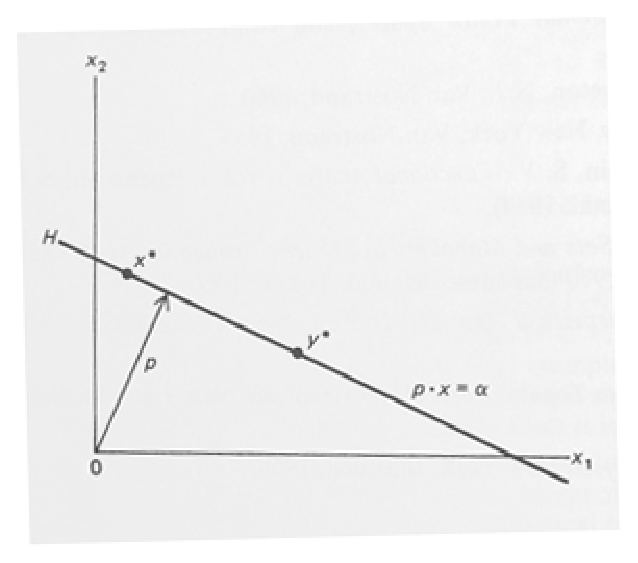
\includegraphics[width=0.47\textwidth]{line}}\hfill
\subfigure[Плоскость]{\includegraphics[width=0.47\textwidth]{3dplane}}
\caption{Примеры гиперплоскостей}\label{fig:Hplanes_exam}
\end{figure}



Изменяя значение $\gamma$ (сдвигая гиперплоскость), мы получаем
целое семейство гиперплоскостей (см. Рис.~\ref{fig:hypermap}).

\input{pics/hypermap.TpX}


    Важнейшая роль выпуклых множество в математической экономике и теории экстремальных задач
    обусловлена тем, что для них справедливы так называемые теоремы отделимости.
    Есть несколько различных формулировок теорем отделимости. Мы приведем здесь только те из них,
    которые понадобятся нам в дальнейшем. Их доказательства мы приводить не будем в надежде на то,
    что геометрически они выглядят довольно правдоподобными.

    Два множества $\st{X}$ и $\st{Y}$ из $\R^n$ называются
    \emph{отделимыми}, если существует такая гиперплоскость
    $\st{H}_{p,\gamma}$, называемая \emph{разделяющей}, что множество
    $\st{X}$ лежит в одном
    из замкнутых полупространств, порожденных этой гиперплоскостью,
    а множество $\st{Y}$ --- во втором. Иными словами, множества $\st{X}$ и
    $\st{Y}$ отделимы, если существуют такой ненулевой линейный функционал $p(\vc{x})$,
    и число $\gamma$, что
\[
    p(\vc{x})\leq\gamma\leq p(\vc{y}) \ \forall \vc{x}\in\st{X} \ \forall \vc{y}\in\st{Y}.
\]




\begin{teo}[отделимости]
  \label{teo-otd-1}
    Предположим, что $\st{X}$ и $\st{Y}$ --- выпуклые множества из
    $\R^n$, причем хотя бы одно из них, скажем, $\st{Y}$, имеет
    непустую внутренность (\remrk{что такое внутренность????}) $\emph{int}\st{Y}$. Если
    $\st{X}\cap\emph{int}\st{Y}=\emptyset$, то множества $\st{X}$ и
    $\st{Y}$ отделимы.
\end{teo}

     Подчеркнем, что в
    сформулированной теореме не требуется, чтобы множества не пересекались. Важно, чтобы
    одно из двух множеств не пересекалось с внутренностью другого, если, конечно, эта
    внутренность сама не являлась пустым множеством (см. \remrk{РИС}).
    Безусловно, предположение о том, что оба множества, $\st{X}$ и $\st{Y}$,
    являются выпуклыми, является крайне существенным, что проиллюстрировано \remrk{РИС}.


    Пусть $\st{X}$ --- некоторое множество из $\R^{n}$ и точка
    $\vc{\hat{x}}$ принадлежит границе этого множества. Гиперплоскость
    $\st{H}_{p,\gamma}$ называется \emph{опорной} к множеству $\st{X}$
    в точке $\vc{\hat{x}}$, если эта точка принадлежит
    данной гиперплоскости, а само множество $\st{X}$ содержится в
    полупространстве $\st{H}_{p,\gamma}^{-}$, т.е. если
    \[\gamma=p(\vc{\hat{x}})\geq p(\vc{x}) \ \forall x\in\st{X}.\]

    Заметим, что последнее неравенство говорит, в частности, что
    если точка $\vc{\hat{x}}$  принадлежит множеству $\st{X}$
    (а это действительно так, если это множество замкнуто),
    то она  представляет собой решение задачи
\begin{equation}
    \label{max-lin-na-vip}
    p(\vc{x})\rightarrow\max, \ \vc{x}\in\st{X},
\end{equation}
    причем значением этой задачи является число $\gamma$. Подчеркнем также,
    что, формально говоря, опорная к множеству $\st{X}$
    в точке $\vc{\hat{x}}$ гиперплоскость представляет собой
    гиперплоскость, разделяющую множество $\st{X}$ и множество,
    состоящее из единственной точки $\vc{\hat{x}}$ (\remrk{РИС}).

\begin{teo}[об опорной гиперплоскости]
    \label{teo-op-gip}
    Если $\st{X}$ --- выпуклое множество, то для любой его граничной (\remrk{????})
    точки $\vc{\hat{x}}$  найдется гиперплоскость, опорная в этой точке
    к данному множеству.
\end{teo}

    Из теоремы об опорной гиперплоскости следует, что любая
    граничная точка выпуклого замкнутого множества $\st{X}$ представляет
    собой решение некоторой задачи вида (\ref{max-lin-na-vip}). В то
    же время, очевидно, что любое решение такой задачи является
    граничной точкой $\st{X}$. Заметим, что в случае, когда
    множество $\st{X}$ имеет непустую внутренность, теорема об
    опорной гиперплоскости вытекает из теоремы отделимости.

    Далее нам понадобится еще одна теорема, которая говорит, что
    если точка $\vc{\hat{x}}$ не принадлежит выпуклому замкнутому
    множеству $\st{X}$, то $\vc{\hat{x}}$ <<строго>> отделима от
    $\st{X}$ с помощью некоторой гиперплоскости $\st{H}_{p,\gamma}$ (\remrk{РИС ?????}).


\begin{teo}\label{strog-otdotochki}
    Пусть $\st{X}$ --- выпуклое замкнутое множество, а точка
    $\vc{\hat{x}}$  не принадлежит $\st{X}$. Тогда существует такой
    ненулевой линейный функционал $p(\vc{x})$ и число
     $\gamma$, такие что
    \[p(\vc{x})<p(\vc{\hat{x}}) \ \forall \vc{x}\in\st{X}.\]
\end{teo}

\begin{exer}
    Докажите, что любое замкнутое выпуклое множество $\st{X}$ представляет
    собой пересечение всех полупространств
    $\st{H}_{p,\gamma}^{-}$, порождаемых опорными к $\st{X}$
    гиперплоскостями.


\end{exer}


\section{Лемма Фаркаша}

    В качестве приложения одной из только что сформулированных теорем, докажем важную
    лемму Фаркаша, которую мы уже использовали в предыдущей главе для доказательства
    некоторых теорем линейного программирования.


    Множество $\st{X}\subset\R^{n}$ называется \emph{\textbf{конусом}}, если для
    любого вектора $\vc{x}\in\st{X}$ и любого числа
    $\lambda\geqslant0$ справедливо включение
     $\lambda\vc{x}\in\st{X}$, т.е. если вместе с любой своей точкой множество
     $\st{X}$ вместе с любой своей точкой содержит проходящий через
     нее луч с началом в нуле (см. рис. ?????, а)
     Если конус $\st{X}$ является выпуклым
     множеством, то он называется \emph{\textbf{выпуклым конусом}} (см. рис. ?????, b).
     Простейшим примером выпуклого конуса является множество $\R_{+}^{n}$.


\begin{exer}
    Докажите, что
    \begin{itemize}
      \item множество $\st{X}$ является выпуклым конусом
    тогда и только тогда, когда для любых векторов $\vc{x'}\in\st{X}$
    и $\vc{x''}\in\st{X}$ и любых чисел $\lambda'\geqslant0$ и
    $\lambda''\geqslant0$ справедливо включение
    $\lambda'\vc{x'}+\lambda''\vc{x''}\in\st{X}$;
      \item пересечение любого числа выпуклых конусов является выпуклым
      конусом;
      \item объединение любого числа выпуклых конусов является конусом,
      но необязательно выпуклым.
    \end{itemize}

\end{exer}


    Пусть $\vc{a^{1}},\ldots,\vc{a^{m}}$ --- конечный набор векторов из
    $\R^{n}$. Вектор вида
    \[\lambda_{1}\vc{a^{1}}+\ldots+\lambda_{m}\vc{a^{m}}\] называется
    \textbf{\emph{линейной комбинацией}} этих векторов. Эта
    линейная комбинация называется \emph{\textbf{неотрицательной}}, если
    $\lambda_{1}\geqslant0,\ldots,\lambda_{m}\geqslant0$ и \emph{\textbf{выпуклой}},
    если $\lambda_{1}\geqslant0,\ldots,\lambda_{m}\geqslant0$ и
    $\lambda_{1}+\ldots+\lambda_{m}=1$. Напомним, что понятие выпуклой комбинации двух точек
    мы уже использовали.




\begin{exer}\label{vipukl-konus}
    Докажите, что
\begin{itemize}
      \item
      множество всевозможных неотрицательных линейных комбинаций конечного набора
      векторов является выпуклым конусом;
      \item
      множество всевозможных выпуклых комбинаций конечного набора
      векторов является выпуклым множеством;
 \end{itemize}
\end{exer}

    Множество всевозможных линейных неотрицательных комбинаций
    конечного набора векторов $\vc{a^{1}},\ldots,\vc{a^{m}}$
    называется конусом, \emph{\textbf{натянутым}} на эти вектора.


    Для доказательства леммы Фаркаша нам понадобится следующая
    техническая лемма. Доказательство этой леммы является несложным, но
    довольно длинным. Поэтому мы его опускаем в надежде на то, что
    сама ее формулировка представляется читателю вполне
    естественной.

\begin{lem}\label{zamkn-konus}
    Конус, натянутый на любой конечный набор векторов, является
    замкнутым множеством.
\end{lem}


    Перейдем к формулировке и доказательству леммы Фаркаша.


\begin{teop}(лемма Фаркаша) \label{lemma-F1}
    Предположим, что нам задан конечный набор векторов
    \[\vc{a_{1}},\ldots,\vc{a_{m}},\]
    лежащих в конечномерном пространстве ${\R}^{n}$. Для любого
    вектора $\vc{d}$ из ${\R}^{n}$ справедлива одна и только одна из двух
    следующих альтернатив:
\begin{itemize}
    \item [1)\ ] либо найдутся числа
    $v_{1}\geq0,\ldots,v_{m}\geq0$, такие что
    \[\vc{d}=v_{1}\vc{a_{1}}+\ldots+v_{m}\vc{a_{m}};\]

    \item [2)\ ] либо существует такой линейный функционал $h(\cdot)$,
    заданный на ${\R}^{n}$, что одновременно выполняются следующие неравенства:
    \[h(\vc{a_{1}})\leq0,\ldots,h(\vc{a_{m}})\leq0,\]
    \[h(\vc{d})>0.\]
\end{itemize}
\end{teop}

    \emph{\textbf{Доказательство.}}
    Рассмотрим конус $\mathbb{K}$, натянутый на вектора
    $\vc{a_{1}},\ldots,\vc{a_{m}}$. Этот конус является выпуклым
    (см. упражнение \ref{vipukl-konus}) и, по
    лемме \ref{zamkn-konus}, замкнутым.

    Возможно одно и только одно из двух следующих соотношений: либо $\vc{d}\in\mathbb{K}$,
    либо $\vc{d}\notin\mathbb{K}$. Включение  $\vc{d}\in\mathbb{K}$
    эквивалентно существованию (\remrk{РИС ?????}) таких неотрицательных чисел
    $v_{1}\geq0,\ldots,v_{m}\geq0$, что
    \[\vc{d}=v_{1}\vc{a_{1}}+\ldots+v_{m}\vc{a_{m}}.\]

    Что касается соотношения $\vc{d}\notin\mathbb{K}$, то с учетом
    теоремы \ref{strog-otdotochki}, оно эквивалентно существованию
    такого линейного функционала $h(\vc{x})$ (\remrk{РИС ?????}), заданного на пространстве $\R^{n}$,
    для которого выполняется следующее соотношение:
\[
    h(\vc{x})< h(\vc{d}) \ \forall \vc{x}\in\mathbb{K}.
\]
    Поскольку $\vc{0}\in\mathbb{K}$, мы имеем: $h(\vc{d})>0$.

    Покажем, что
\[
    h(\vc{x})\leqslant0 \ \forall \vc{x}\in\mathbb{K}.
\]
    Действительно, предположим, что $h(\vc{\bar{x}})>0$ для некоторого
    $\vc{\bar{x}}\in\mathbb{K}$. В этом случае при достаточно
    большом $\lambda>0$ одновременно выполняется неравенство
    $h(\lambda\vc{\bar{x}})>h(\vc{d})$ и включение
    $\lambda\vc{\bar{x}}\in\mathbb{K}$, чего быть не может.

    Нам осталось заметить, что $\vc{a_{j}}\in\mathbb{K}, \ j=1,\ldots,m$ и, значит,
    $h(\vc{a_{j}})\leqslant0, \ j=1,\ldots,m$.
    $\Box$

    Важным следствием доказанной теоремы является следующая лемма.

\begin{lem}\label{lemma-F2}
    Предположим, что нам заданы $r\times s$ матрица $\vc{A}$ и
    $r$-мерный вектор-столбец $\vc{d}$. Справедлива ровно одна из двух
    следующих альтернатив:
\begin{itemize}
    \item [1)\ ] либо найдется $s$-мерный вектор-столбец $\vc{v}\geqq\vc{0}$,
    такой что
    \[\vc{d}=\vc{A}\vc{v};\]

    \item [2)\ ] либо существует такая вектор-строка $\vc{h}$, что
    одновременно выполняются следующие неравенства:
    \[\vc{h}\vc{A}\leqq0, \ \vc{h}\vc{d}>0.\]
    \end{itemize}
\end{lem}
    \textbf{\emph{Доказательство.}}
    Рассмотрим набор $r$-мерных
    вектор-столбцов $\vc{a_{1}},\ldots,\vc{a_{s}}$,  из которых состоит матрица
    $\vc{A}$, и $r$-мерный вектор-столбец $\vc{d}$. По теореме
    \ref{lemma-F1} выполняется ровно одна из двух следующих
    альтернатив:

    --- либо существует такой неотрицательный $s$-мерный
    вектор-столбец
    $\vc{v}=\left(
              \begin{array}{c}
                v_{1} \\
                \vdots \\
                v_{s} \\
              \end{array}
            \right)$,
            что
       \[\vc{d}=v_{1}\vc{a_{1}}+\ldots+v_{s}\vc{a_{s}}=\vc{A}\vc{v},\]
    --- либо найдется такой линейный функционал $h(\vc{x})$,
    заданный на ${\R}^{r}$, что одновременно выполняются следующие неравенства:
    \[h(\vc{d})>0,\]
  \[h(\vc{a_{1}})\leq0,\ldots,h(\vc{a_{m}})\leq0.\]
    Рассмотрим вторую альтернативу.
    Как мы помним, всякий линейный функционал, заданный на пространстве
    $\R^{r}$, состоящем из вектор-столбцов, однозначным образом
    задается некоторой $r$-мерной вектор-строкой. Применительно к
    линейному функционалу $h(\vc{x})$ это значит, что существует
    такая вектор-строка $\vc{h}=(h_{1},\ldots,h_{r})$, что для любого
    вектора $\vc{x}\in\R^{r}$ выполняется равенство
    $\vc{h}\vc{x}=h(\vc{x})$. Для этой вектор-строки мы имеем:
\[
    \vc{h}\vc{d}>0,
\]
\[
    \vc{h}\vc{a_{1}}\leq0,\ldots,\vc{h}\vc{a_{s}}\leq0,
\]
    причем последний набор неравенств мы компактно можем переписать
    в следующем виде:
\[
    \vc{h}\vc{A}\leqq0. \Box
\]

\begin{exer}
    Докажите следующую лемму.
\end{exer}


\begin{lem}\label{lemma-F3}
    Предположим, что нам заданы $s\times r$ матрица $\vc{A}$ и
    $r$-мерный вектор-столбец $\vc{d}$. Справедлива ровно одна из двух
    следующих альтернатив:
\begin{itemize}
    \item [1)\ ] либо найдется $s$-мерный вектор-строка $\vc{v}\geqq\vc{0}$,
    такая что
    \[\vc{d}=\vc{v}\vc{A};\]

    \item [2)\ ] либо существует такой вектор-столбец $\vc{h}$, что
    одновременно выполняются следующие неравенства:
    \[\vc{A}\vc{h}\leqq0, \ \vc{d}\vc{h}>0.\]
    \end{itemize}
\end{lem}

    Заметим, что в научной и учебной литературе иногда под леммой Фаркаша понимают не теорему
    \ref{lemma-F1}, а лемму \ref{lemma-F2} или лемму \ref{lemma-F3}










\newpage

\section{Эффективные точки}

Важную роль в экономическом анализе играет понятие эффективности,
которое несколько отличается от обыденного представления об
эффективности.


УТОЧНИТЬ ОПРЕДЕЛЕНИЯ!!!!!

\begin{dfn}

    Точка ${\vc{\hat x}} \in \st{X} \subset \R^n$ называется

\begin{enumerate}
  \item \textbf{эффективной} точкой множества $\st{X}$, если не существует другой точки $\vc{x} \in
\st{X}$, такой, что $\vc{x} \geq \vc{\hat x}$;

  \item \textbf{слабо эффективной} точкой
множества $\st{X}$, если не существует другой точки $\vc{x} \in
\st{X}$, такой, что $\vc{x} \gg \vc{\hat x}$.

\end{enumerate}
\end{dfn}

    Чтобы пояснить введенные определения, напомним, какой смысл
    имеют неравенства $\geq$ и $\gg$ применительно к векторам. Для
    векторов $\vc{x}=(x_{1},...,x_{n})$ и $\vc{y}=(y_{1},...,y_{n})$
    из пространства $\R^{n}$ неравенство $\vc{x}\gg\vc{y}$
    означает, что
\[
    x_{i}>y_{i}, \ i=1,...,n,
\]
    неравенство $\vc{x}\geqq\vc{y}$ говорит о том, что
\[
    x_{i}\geqslant y_{i}, \ i=1,...,n,
\]
    а соотношение $\vc{x}\geq\vc{y}$ --- о том, что выполняются последние неравенства и $x_{i}>y_{i}$
    хотя бы для одного $i$.
    Мы видим, что точка
    ${\vc{\hat x}} \in \st{X}$ является слабо эффективной, если \emph{не
    найдется} другой точки $\vc{x}$ из множества $\st{X}$,
    превосходящей ${\vc{\hat x}}$ по всем координатам. Точка
    ${\vc{\hat x}} \in \st{X}$ является эффективной, если не найдется другой
    точки $\vc{x}\in\st{X}$, которая не меньше ${\vc{\hat x}}$ по
    всем координатам, причем хотя бы по одной --- строго больше.






Из приведенного выше определения нетрудно видеть, что любая эффективная точка является и
слабо эффективной. Если точка не является слабо эффективной, то она не может быть и
эффективной. В то же время, из того факта, что точка ${\vc{\hat x}}$ является слабо
эффективной, не следует, что она эффективна. (\remrk{РИС?????})





\begin{prop}\label{vzvesh-summa}

Пусть $\st{X} \subset \R^n$ и пусть вектор $\vc{\hat x}$ представляет собой решение задачи

\begin{equation}\label{eq:eff_conditions}
\left\{ \begin{array}{l}
 \vc{p}\vc{x} = p_1x_1 + \ldots + p_n x_n\to \max  \\
 \vc{x} \in \st{X}, \\
 \end{array} \right.
\end{equation}



\begin{enumerate}
\renewcommand{\theenumi}{(\roman{enumi})}
  \item Если $\vc{p} \geq \vc{0}$, то точка $\vc{\hat x} \in \st{X}$ является
  слабо эффективной.
  \item Если $\vc{p} \gg \vc{0}$, то точка $\vc{\hat x} \in \st{X}$ является
  эффективной.
\end{enumerate}

\end{prop}

\begin{proof}

(i) Предположим, что утверждение данного пункта не выполняется. В
этом случае существует $\vc{\bar x} \in \st{X}$ такой, что $\vc{\bar
x} \gg \vc{\hat x}$. Тогда, поскольку $\vc{p} \geq \vc{0}$, получаем
$\vc{p}\vc{\bar x} > \vc{p}\vc{\hat x}$. Однако это противоречит
тому факту, что $\vc{\hat x}$ есть решение задачи
(\ref{eq:eff_conditions}).

(ii) Докажите самостоятельно в качестве \textbf{упражнения}.

\end{proof}



Отметим, что в приведенном предложении не накладывается никаких требований к устройству
множества $\st{X}$. В некотором смысле обратное утверждение требует выпуклости множества
$\st{X}$.



\begin{prop}\label{usl-eff}

Пусть $\st{X} \subset \R^n$ --- выпуклое множество. Если точка ${\vc{\hat x} \in \st{X}}$
является слабо эффективной точкой множества $\st{X}$, то существует вектор ${\vc{p} \geq
\vc{0}}$ из $\R^n$, такой что
\[\vc{p}\vc{\hat x}\geq\vc{p}\vc{x} \ \forall \vc{x}\in\st{X},\]
т.е. $\vc{\hat x}$ есть решение задачи (\ref{eq:eff_conditions}).
\end{prop}

\begin{proof}
Положим
\[
    \st{Y}=\{\vc{y} \in \R^n: \vc{y} \geqq \vc{\hat x}\}.
\]
Множество $\st{Y}$ является выпуклым, причем, как легко проверить,
\[
    \text{int}\st{Y}=\{\vc{y} \in \R^n: \vc{y} \gg \vc{\hat x}\}.
\]

 Поскольку $\vc{\hat x}$
является слабо эффективной точкой множества $\st{X}$, то, как легко заметить,
 $\st{X}\cap\text{int}\st{Y}=\emptyset$. Таким образом, мы имеем два непересекающихся
 выпуклых множества, $\st{X}$ и $\st{Y}$, причем таких, что первое из них не пересекается
 с непустой внутренностью второго (\remrk{РИС?????}).

Значит, по теореме отделимости (теореме \ref{teo-otd-1}) найдутся
ненулевой вектор $\vc{p}=(p_{1},...,p_{n})\in \R^n$ и число
    $\gamma\in \R$ такие, что для любого $\vc{x} \in \st{X}$ и любого $\vc{y}
\in \st{Y}$ выполняются следующие соотношения:

\[
\vc{p} \cdot \vc{x} \leq \gamma \leq \vc{p} \cdot \vc{y}.
\]

    Проверим, что $\vc{p} \geq \vc{0}$. Для этого предположим, что
 это не так и, тем самым, $p_i <0$ для некоторого $i$. Обозначим
 через $\vc{e_{i}}$ вектор из $\R^{n}$, все координаты
 которого, за исключением $i$-й, равны $0$, а $i$-я координата равна
 $1$. Очевидно, $\vc{p}\vc{e_{i}}=p_{i}<0$
    и, следовательно, $\vc{p}(\vc{\hat x}+\vc{e_{i}})<\vc{p}\vc{\hat x}$.
    А этого быть не может, поскольку вектор $\vc{\hat x}+\vc{e_{i}}$ содержится в $\st{Y}$.

    Нам осталось заметить, что, поскольку $\vc{\hat x}$ содержится как в $\st{X}$, так и в
    $\st{Y}$, мы имеем
    $\vc{p} \cdot \vc{\hat x}=\gamma$.
    А это означает, что
    $\vc{\hat x}$ есть решение задачи (\ref{eq:eff_conditions}).
\end{proof}

    Из двух сформулированных предложений вытекает следующая теорема.

\begin{teop}\label{neob-dosti-usl-eff}
    Пусть $\st{X} \subset \R^n$ --- выпуклое замкнутое множество.
    Вектор ${\vc{\hat x} \in \st{X}}$ является слабо эффективной точкой
    множества $\st{X}$ тогда и только тогда, когда то существует вектор
    ${\vc{p} \geq \vc{0}}$, $\vc{p} \in \R^n$, такой что
    \[\vc{p}\vc{\hat x}\geq\vc{p}\vc{x} \ \forall \vc{x}\in\st{X},\]
    т.е. $\vc{\hat x}$ есть решение задачи (\ref{eq:eff_conditions}).
\end{teop}



  Напомнив, что всякая эффективная точка
  является и слабо эффективной, отметим, что нельзя сформулировать аналогичные
  необходимые и достаточные условия эффективности.
  Действительно, из того факта, что точка
  является эффективной, вовсе не следует, что соответствующий вектор $\vc{p} \gg \vc{0}$. В
  качестве примера на Рис.~\ref{fig:circle_eff} приведем окружность (выпуклое
  множество), точка $A$ которой очевидным образом является
  эффективной, но $\vc{p} \geq \vc{0}$. (В качестве \textbf{упражнения}
  аккуратно докажите этот факт).

\input{pics/circle_eff.TpX}




\begin{exer}
  \label{neper-pol-ort}
    Докажите, что выпуклое множество $\st{X}$ не пересекается с множеством
    $\{\vc{x}\in \R^{n} \mid  \vc{x}\gg \vc{0} \}$ тогда и только тогда, когда существует
    вектор
    ${\vc{p} \geq \vc{0}}$, $\vc{p} \in \R^n$, такой что
\[
    \vc{p}\vc{x}\leq 0 \ \forall \vc{x}\in \st{X}.
\]


\end{exer}

\begin{exer}
    Пусть
    $\st{X}=\{\vc{x}=(x_{1},x_{2})\in\R_{+}^{2}\mid
    x_{1}^{2}+x_{2}^{2}\leqslant25\}$,
    $\vc{\hat{x}}=(3,4)$. Докажите, что точка $\vc{\hat{x}}$
    эффективна и укажите коэффициенты $p_{1}$ и $p_{2}$ при которых
    эта точка является решением задачи (\ref{eq:eff_conditions}).


\end{exer}






Стандартный пример выпуклого множества, приводимый в элементарных учебниках по экономической
теории --- множество производственных возможностей экономики, ограниченное \dw{кривой
производственных возможностей} (англ., \emph{production possibility
frontier}\footnote{\cite{McConnell:1996}}). См. Рис.~\ref{fig:ppfrontier}, где изображены
множество производственных возможностей и граница производственных возможностей экономики,
производящей два вида товаров: пушки и масло. Граница производственных возможностей --- это,
как уже заметил читатель, множество всех слабо эффективных точек множества производственных
возможностей. Теорема \ref{neob-dosti-usl-eff} применительно к данному примеру говорит о том,
что некоторый вектор выпускаемых продуктов принадлежит границе производственных возможностей
тогда и только тогда, когда этот вектор доставляет максимум валового внутреннего продукта на
всем множестве производственных возможностей экономики при некотором векторе цен на
выпускаемые продукты. Очевидно, что разным векторам цен соответствуют, вообще говоря,
различные точки на границе производственных возможностей.


\input{pics/ppfrontier.TpX}


Рис.~\ref{fig:ppfrontier} \emph{а)},

На Рис.~\ref{fig:ppfrontier} \emph{б)}  Рис.~\ref{fig:ppfront_max}.

\input{pics/ppfront_max.TpX}






\subsection{Выпуклые и вогнутые функции}

    Теперь перейдем к описанию основных свойств выпуклых и вогнутых функций, которые играют
    ключевую роль в математической экономике и экономической теории в целом.


\begin{dfn}
Пусть нам дано выпуклое множество $\st{X} \subset \R^n$. Функция
    $f: \st{X} \to \R$ называется

\begin{enumerate}
\renewcommand{\theenumi}{(\asbuk{enumi})}

  \item  \dw{вогнутой}\index{вогнутая функция},
если для любых $\vc{x}', \vc{x}'' \in \st{X}$ и $0 \leq \theta \leq
1$ выполняется (см. Рис. \ref{fig:concave-function})

\[
    f[\theta \vc{x}' + (1-\theta)\vc{x}'] \geq \theta f(\vc{x}') +
    (1-\theta)f(\vc{x}'').
\]

  \item \dw{строго вогнутой}\index{строго вогнутая функция},
если для любых $\vc{x}', \vc{x}'' \in \st{X}$, $\vc{x}' \neq
\vc{x}''\!$, и $0 < \theta < 1$ выполняется

\[
f[\theta \vc{x}' + (1-\theta)\vc{x}''] > \theta f(\vc{x}') +
(1-\theta)f(\vc{x}'').
\]

  \item \dw{выпуклой}\index{выпуклая функция},
если для любых $\vc{x}', \vc{x}'' \in \st{X}$ и $0 \leq \theta \leq
1$ выполняется

\[
f[\theta \vc{x}' + (1-\theta)\vc{x}''] \leq \theta f(\vc{x}') +
(1-\theta)f(\vc{x}'').
\]

\item \dw{строго выпуклой}\index{строго выпуклая функция},
если для любых $\vc{x}', \vc{x}'' \in \st{X}$, $\vc{x}' \neq
\vc{x}''\!$, и $0 < \theta < 1$ выполняется

\[
f[\theta \vc{x}' + (1-\theta)\vc{x}''] < \theta f(\vc{x}') +
(1-\theta)f(\vc{x}'').
\]

\end{enumerate}
\end{dfn}


\begin{figure} \centering
   \includegraphics[width=10cm]{concave_function}\\
  \caption{Вогнутая функция}\label{fig:concave-function}
\end{figure}


    \remrk{НА РИС} изображены строго выпуклая и строго вогнутая функции, а выпуклая функция,
    не являющаяся строго выпуклой, и вогнутая функция, не являющаяся строго вогнутой.



\begin{dfn}
    Пусть $\st{X}\subset\R^{n}$.
 \dw{Надграфиком} функции $f:\st{X}\rightarrow \R$ называется множество
    \[
    \st{G}_{f}^+=\{ (\vc{x}, \gamma) \in \R^{n+1}: \vc{x}\subset\st{X}, \
    f(\vc{x}) \leq \gamma \},
    \]
    а \dw{подграфиком} --- множество
    \[
    \st{G}_{f}^- =\{ (\vc{x}, \gamma) \in \R^{n+1}: \vc{x}\subset\st{X}, \
    f(\vc{x}) \geq \gamma \}.
    \]
\end{dfn}

\remrk{? Как обозначить лебегово множество}



\begin{exer}
Докажите следующие утверждения.


\begin{enumerate}
\renewcommand{\theenumi}{(\roman{enumi})}

  \item Функция $f(\vc{x})$ является выпуклой
(строго выпуклой) тогда и только тогда, когда функция $-f(\vc{x})$
является вогнутой (строго вогнутой).

  \item Линейная функция является и вогнутой, и выпуклой, но не является строго вогнутой или
  строго выпуклой.

  \item
  Если функции $f_{j}(\vc{x}), \ j=1,...,m,$ вогнуты (выпуклы), то
  при любых неотрицательных числах $\lambda_{1},...,\lambda_{m}$
  вогнута (выпукла) и функция
  $f(\vc{x})=\lambda_{1}f_{1}(\vc{x})+...+\lambda_{m}f_{m}(\vc{x})$
  (неотрицательная линейная комбинация вогнутых функций также
  вогнута, а выпуклых --- выпукла).


  \item Функция является выпуклой (вогнутой) тогда и только тогда,
  когда ее надграфик (подграфик) является выпуклым множеством.

  \item Функция $f(\vc{x})$, заданная на выпуклом множестве $\st{X}$,
  является выпуклой (вогнутой) тогда и только тогда,
  когда для любого целого числа $m \geq 1$, для любых векторов
  $\vc{x}^j \in \st{X}, \ j=1,..,m,$ и любых таких неотрицательных чисел
  $\theta_j \geq 0, \ j=1,\ldots,m,$ что
  $\theta_{1}+...+\theta_{m}=1$, выполняется \emph{неравенство Йенсена}:
  \[
    f(\theta_1 \vc{x}^1 +...+\theta_m
    \vc{x}^m) \leq \theta_1 f(\vc{x}^1)+\ldots +\theta_m
    f(\vc{x}^m)
  \]
  \[
    (f(\theta_1 \vc{x}^1 +...+\theta_m
    \vc{x}^m) \geq \theta_1 f(\vc{x}^1) + \ldots +\theta_m
    f(\vc{x}^m))
  \]

    \item Функция $f:\st{X}\rightarrow \R$ является вогнутой тогда и только тогда, когда
    выпуклым является множество
\[
    \st{G}_{f}^+=\{ (\vc{x}, \gamma) \in \R^{n+1}: \vc{x}\subset\st{X}, \
    f(\vc{x}) \leq \gamma \},
\]
    (оно называется надграфиком функции $f$)

    \item Функция $f:\st{X}\rightarrow \R$ является выпуклой тогда и только тогда, когда
    выпуклым является множество
\[
    \st{G}_{f}^- =\{ (\vc{x}, \gamma) \in \R^{n+1}: \vc{x}\subset\st{X}, \
    f(\vc{x}) \geq \gamma \}.
\]
    (оно называется подграфиком функции $f$)

  \item Если функции $f_{j}(\vc{x}), \ j=1,...,m,$ являются
  выпуклыми, то функция
  $f(\vc{x})=\min\limits_{j}f_{j}(\vc{x})$
  тоже выпукла.
  Если функции $f_j (\vc{x}), j=1, \ldots, m$, являются
  вогнутыми, то функция
  $f(\vc{x}) = \mathop {\min }\limits_j f_j(\vc{x})$ также вогнута.

\end{enumerate}

\end{exer}

\remrk{ПЕРЕНЕСТИ В СЛЕД ГЛАВУ:}

\remrk{Следующее предложение иллюстрируется РИС???}



\begin{prop}
    Если в некоторой точке $\vc{\hat x}$ выпуклого множества $\st{X}$
    достигается локальный максимум (минимум) вогнутой  (выпуклой)
    функции $f(\vc{x})$, то в этой же
  точке достигается и глобальный максимум  (минимум).
\end{prop}
    \textbf{Доказательство.} Мы проведем доказательство для случая локального
    максимума вогнутой функции. Пусть $\vc{\hat x}$ --- точка
    локального максимума. Это означает, что существует такая
    $\epsilon$-окрестность $\mathcal{U}_{\epsilon}(\vc{\hat x})$ ($\epsilon>0$) точки
    $\vc{\hat x}$, что
\[
    f(\vc{\hat x})\geqslant f(\vc{x}) \
    \forall \vc{x}\in\st{X}\cap\mathcal{U}_{\epsilon}(\vc{\hat x})
\]
    Возьмем произвольную точку $\vc{x}\in\st{X}$. Поскольку и
    $\vc{\hat x}$, и $\vc{x}$ принадлежит множеству $\st{X}$, причем
    это множество выпукло,
\[
    \vc{\bar{x}}=(1-\lambda)\vc{\hat{x}}+\lambda\vc{x}
    \in\st{X}\cap\mathcal{U}_{\epsilon}(\vc{\hat x})
\]
    при достаточно малом $\lambda>0$ и, следовательно, с учетом
    определения вогнутой функции,
\[
    f(\vc{\hat{x}})\geqslant f(\vc{\bar{x}})= f((1-\lambda)\vc{\hat{x}}+\lambda\vc{x})
    \geqslant(1-\lambda)f(\vc{\hat{x}})+\lambda f(\vc{x}),
\]
    откуда вытекает неравенство $\lambda f(\vc{\hat{x}})\geqslant \lambda f(\vc{x}).$

    Тем самым, с учетом произвольности выбора точки $\vc{x}$,
\[
    f(\vc{\hat{x}})\geqslant f(\vc{x}) \ \forall \vc{x}\in\st{X},
\]
    что и требуется. $\Box$

\remrk{Следующее предложение иллюстрируется РИС???}

\begin{prop}
    Предположим, что функция $f(\vc{x})$ задана на выпуклом множестве
    $\st{X}$  и дифференцируема в точке $\vc{\hat x} \in \st{X}$.
    Если функция $f(\vc{x})$ выпукла, то
\[
    f(\vc{x}) \geqslant f(\vc{\hat x}) + \nabla f(\vc{\hat x}) \cdot
    (\vc{x}-\vc{\hat x}) \ \forall \vc{x} \in  \st{X},
\]
    а если вогнута, то
\[
    f(\vc{x}) \leqslant f(\vc{\hat x}) + \nabla f(\vc{\hat x}) \cdot
    (\vc{x}-\vc{\hat x}) \ \forall \vc{x} \in  \st{X}.
\]
\end{prop}
    \textbf{Доказательство.} Мы рассмотрим случай, когда функция $f(\vc{x})$
    выпукла.
    Зафиксируем $\vc{x} \in  \st{X}$ и положим $\vc{h}=\vc{x}-\vc{\hat x}$.
    Поскольку множество $\st{X}$ выпукло, точка
    $\vc{\hat x}+\alpha\vc{h}=\alpha\vc{x}+(1-\alpha)\vc{\hat x}$
    принадлежит этому множеству при всех $\alpha\in(0,1)$. В силу
    дифференцируемости (\remrk{ЧТО ЕСТЬ ДИФФЕРЕНЦИРУЕМОСТЬ???}) функции $f(\vc{x})$  в точке $\vc{\hat x}$, при
    достаточно малых $\alpha\in(0,1)$ мы имеем:
\begin{multline*}
    f(\alpha\vc{x}+(1-\alpha)\vc{\hat x})
    =f(\vc{\hat x}+\alpha\vc{h})= \\
    =f(\vc{\hat x})+\nabla f(\vc{\hat x})(\alpha\vc{h})+o(\|\alpha\vc{h}\|)
    =f(\vc{\hat x})+\alpha\nabla f(\vc{\hat x})\vc{h}+o(\alpha)\|\vc{h}\|,
\end{multline*}
    а в силу выпуклости этой функции,
\[
    f(\alpha\vc{x}+(1-\alpha)\vc{\hat x})\leqslant
    \alpha f(\vc{x})+(1-\alpha)f(\vc{\hat x})
\]
    и, следовательно,
\[
    \alpha f(\vc{x})+(1-\alpha)f(\vc{\hat x})
    \geqslant f(\vc{\hat x})+\alpha\nabla f(\vc{\hat x})\vc{h}+o(\alpha)\|\vc{h}\|,
\]
    т.е.
\[
    \alpha(f(\vc{x})-f(\vc{\hat x}))
    \geqslant \alpha\nabla f(\vc{\hat x})(\vc{x}-\vc{\hat x})+o(\alpha)\|(\vc{x}-\vc{\hat x})\|.
\]
    Переходя в этом неравенстве к пределу при $\alpha\rightarrow 0$,
    получаем неравенство
\[
    f(\vc{x})-f(\vc{\hat x})\geqslant \nabla f(\vc{\hat x})(\vc{x}-\vc{\hat
    x}),
\]
    откуда и вытекает требуемое.    $\Box$

    Справедливо и в некотором смысле обратное утверждение, а именно,
    имеет место следующее предложение.

\begin{prop}
    Предположим, что функция $f(\vc{x})$ задана  на выпуклом открытом множестве
    $\st{X}$  и дифференцируема на этом множестве. Если для любых
    точек $\vc{x}$ и $\vc{y}$ из $\st{X}$ выполняется неравенство
\[
    f(\vc{x}) \geqslant f(\vc{y}) + \nabla f(\vc{y}) \cdot
    (\vc{x}-\vc{y}) \ \forall \vc{x} \in  \st{X},
\]
    то функция $f(\vc{x})$ выпукла, то а если неравенство
\[
    f(\vc{x}) \leqslant f(\vc{y}) + \nabla f(\vc{y}) \cdot
    (\vc{x}-\vc{y}) \ \forall \vc{x} \in  \st{X},
\]
    то вогнута. $\Box$
\end{prop}


\begin{exer}
    Докажите это предложение.
\end{exer}






\remrk{ПЕРЕНЕСТИ В СЛЕД ГЛАВУ:}



    Напомним, что, согласно теореме \ref{nul-grad-neobh}, если внутренняя точка
    $\vc{x^{*}}$ некоторого множества $\st{D}$ является точкой локального
    максимума или точкой локального минимума дифференцируемой функции $f(\vc{x})$,
    то выполняется равенство $\nabla f(\vc{x^{*}})=\vc{0}$. Из
    доказанного предложения вытекает, что равенство градиента нулю
    представляет собой и достаточное условия максимума в случае,
    когда функция $f(\vc{x})$ вогнута или минимума, если эта функция
    выпукла. А именно, как мы видим, имеет место следующая теорема.

\begin{teo}\label{grad-nul}
    Предположим, что $\st{D}\subset\R^{n}$ --- это выпуклое
    множество, а $\vc{x^{*}}$ --- его внутренняя точка. Предположим
    далее, что функция $f(\vc{x})$, заданная на $\st{D}$, дифференцируема в
    точке $\vc{x^{*}}$.

    Если функция $f(\vc{x})$ вогнута, то
    $\vc{x^{*}}$ представляет собой решение задачи
\[
    f(\vc{x})\rightarrow\max, \ \vc{x}\in\st{D},
\]
    тогда и только тогда, когда $\nabla f(\vc{x^{*}})=\vc{0}$.

    Если функция $f(\vc{x})$ выпукла, то
    $\vc{x^{*}}$ представляет собой решение задачи
\[
    f(\vc{x})\rightarrow\min, \ \vc{x}\in\st{D},
\]
    тогда и только тогда, когда $\nabla f(\vc{x^{*}})=\vc{0}$.
\end{teo}


    Вогнутые и выпуклые функции могут быть и недифференцируемыми. Что касается непрерывности,
    то следует помнить, что справедливо следующее предложение, которые мы приведем без
    доказательства.

\begin{prop}
    Если функция $f(\vc{x})$, заданная на выпуклом множестве $\st{X}$, выпукла или вогнута,
    то она непрерывна на внутренности $\text{\emph{int}}\st{X}$ этого множества.
\end{prop}

\subsection{Квазивыпуклость и квазивогнутость}

    Кроме выпуклых и вогнутых функций экономисту нужно уметь работать с квазивыпуклыми и
    квазивогнутыми функциями.


\begin{dfn}
 Функция $f(\vc{x})$, заданная на выпуклом множестве $\st{X} \in
  \R^n$, называется \dw{квазивогнутой}\index{квазивогнутая функция},
  если для любого $\gamma \in \R$ выпукло множество
\[
    \st{L}^{+}_{f,\gamma}=\{ \vc{x}\in\st{X}: f(\vc{x}) \geq \gamma\},
\]
    и \dw{квазивыпуклой}\index{квазивыпуклая функция},
  если для любого $\gamma \in \R$ выпукло множество
\[
    \st{L}^{-}_{f,\gamma}= \{ \vc{x}\in\st{X}: f(\vc{x}) \leq \gamma \}.
\]
\end{dfn}

    Множество $\st{L}^{+}_{f,\gamma}$, как и множества $\st{L}^{-}_{f,\gamma}$,
    иногда называют \emph{лебеговым множеством} функции $f$. Множество
\[
    \st{L}^{=}_{f,\gamma}= \{ \vc{x}\in\st{X}: f(\vc{x})=\gamma \},
\]
    называют \emph{множеством уровня}. В случае, когда $n=2$,
    множество уровня по понятным причинам называют \emph{линией уровня}.

\remrk{РИС, РИС}


\begin{exer}
Докажите следующие утверждения.


\begin{enumerate}
\renewcommand{\theenumi}{(\roman{enumi})}

  \item Функция $f(\vc{x})$ является квазивыпуклой
    тогда и только тогда, когда функция $-f(\vc{x})$ является
    квазивогнутой.

  \item Всякая выпуклая функция квазивыпукла, а всякая вогнутая ---
  квазивогнута. Обратное, вообще говоря, неверно.



  \item Если функции $f_{j}(\vc{x}), \ j=1,...,m,$ являются
  квазивыпуклыми, то функция
  $f(\vc{x})=\min\limits_{j}f_{j}(\vc{x})$
  тоже квазивыпукла.
  Если функции $f_j (\vc{x}), j=1, \ldots, m$, являются
  квазивогнутыми, то функция
  $f(\vc{x}) = \mathop {\min }\limits_j f_j(\vc{x})$ также квазивогнута.


  \item
  Если функции $f_{1}(\vc{x})$ и $f_{2}(\vc{x})$ квазивогнуты (квазивыпуклы), то
  из этого не следует, что функция
  $f(\vc{x})=f_{1}(\vc{x})+f_{2}(\vc{x})$
  тоже является квазивогнутой (квазивыпуклой).


  \item
  Функция $f(\vc{x})$, заданная на выпуклом множестве $\st{X} \subset
  \R^n$, является квазивыпуклой (квазивогнутой) тогда и только
  тогда, когда для любых векторов $\vc{x'}\in\st{X}$ и
  $\vc{x''}\in\st{X}$ и любого числа $\alpha\in[0,1]$ выполняется
  неравенство
\[
    f(\alpha\vc{x'}+(1-\alpha)\vc{x''})\leqslant\max\{f(\vc{x'}),f(\vc{x''})\}
\]
\[
    f(\alpha\vc{x'}+(1-\alpha)\vc{x''})\geqslant\min\{f(\vc{x'}),f(\vc{x''})\}.
\]

    \item
    Функция $f(x)$, заданная на некотором интервале $(a,b)$ числовой прямой
    $\R$ квазивогнута тогда и только тогда, когда она

    --- либо не убывает на этом промежутке,

    --- либо монотонно не возрастает,

    --- либо существует точка $\hat{x}\in(a,b)$, такая что на
    промежутке $(a,\hat{x}]$ она монотонно не убывает, а на
    промежутке $[\hat{x},b)$ монотонно не возрастает.

    \item Функция
\begin{multline*}
    F(x_{1},\ldots,x_{n})=ax_{1}^{\alpha_{1}}x_{2}^{\alpha_{2}}\ldots x_{n}^{\alpha_{n}}, \ a>0, \\
    \alpha_{1}>0, \ \alpha_{2}>0, \ldots, \alpha_{n}>0, \
    \alpha_{1}+\alpha_{2}+\ldots+\alpha_{n}>1,
\end{multline*}
    является квазивогнутой, но не является вогнутой.


\end{enumerate}


\end{exer}





\subsection{Производственные функции}

        Предположим, что некоторое предприятие производит ровно один вид
         продукции или что выпуск измеряется в денежном выражении.
         Предположим далее, что при производстве продукции необходимо использование
         $n$ различных факторов. В этом случае технологию предприятия удобно
          описывать с помощью производственной функции $F(\vc{x})=F(x_{1},x_{2},...,x_{n})$,
          где $\vc{x}=(x_{1},x_{2},...,x_{n})$. Эта функция показывает максимально возможное
           количество продукции, которое может в течение единичного промежутка времени
           произвести данное предприятие,
           если оно использует первый фактор в количестве $x_{1}$ единиц, второй
           фактор --- в количестве $x_{2}$ единиц, ..., $n$-й фактор --- в количестве $x_{n}$.

           Говоря о какой-нибудь производственной функции $F(\vc{x})$,
           обычно предполагают, и мы тоже будем
           это всегда делать, что она задается на
           множестве  $\R^{n}_{+}$ при некотором целом $n$, принимает
           неотрицательные значения, непрерывна, удовлетворяет равенству
           и \textbf{\emph{монотонно не убывает}} в следующем смысле:
\[
    \vc{x}\geqq\vc{y}\Rightarrow F(\vc{x})\geq F(\vc{y}).
\]
           Иногда (но не всегда) предполагают, что она
           \textbf{\emph{монотонно возрастает}} в следующем смысле:
\[
    \vc{x'}\gg\vc{x''}\Rightarrow F(\vc{x'})>F(\vc{x''}).
\]

\begin{exer}
    Докажите, что всякая монотонно возрастающая производственная
    функция монотонно не убывает.
\end{exer}



            Очень часто берут $n=2$ и используют производственные
            функции вида $F(K,L)$, где $K$ --- это используемый капитал, а $L$ --- это труд.
            Так описывают производственный сектор экономики при
            построении макроэкономических моделей.


             Чаще всего в экономических исследованиях используют производственные
             функции следующих видов:



\begin{multline*}
    F(\vc{x})=F(x_{1},x_{2},...,x_{n})=a_{1}x_{1}+a_{2}x_{2}+...+a_{n}x_{n},
    \\
    a_{1}\geq0,...,a_{n}\geq0, \ \sum_{i=1}^{n}a_{i}>0,
\end{multline*}
     --- линейная производственная функция;
\begin{multline*}
    F(\vc{x})=F(x_{1},x_{2},...,x_{n})=\min\{x_{1}/a_{1},x_{2}/a_{2},...,x_{n}/a_{n}\},     \\
    a_{1}\geq0,...,a_{n}\geq0, \ \sum_{i=1}^{n}a_{i}>0,
\end{multline*}
    --- леонтьевская производственная функция (функция Леонтьева);

\begin{multline*}
    F(\vc{x})=F(x_{1},x_{2},...,x_{n})=
    ax_{1}^{\alpha_{1}}x_{2}^{\alpha_{2}}\ldots x_{n}^{\alpha_{n}},
     \ a>0, \ \alpha_{1}>0,..., \alpha_{n}>0,
\end{multline*}
     --- функция Кобба-Дугласа;

\begin{multline*}
    F(\vc{x})=F(x_{1},x_{2},...,x_{n})
    =(a_{1}x_{1}^{\rho}+\ldots+a_{n}x_{n}^{\rho})^{\alpha/\rho},
    \\ 0\neq\rho<1, \ \alpha>0, \ a_{1}>0,...,a_{n}>0,
\end{multline*}
     --- функция постоянной эластичности замещения (constant elasticity of substitution, CES).



\begin{exer}
    Покажите, что для леонтьевской производственной функции $F(\vc{x})$ справедливо равенство
\[
    \st{L}^{+}_{F,\gamma}=\{\vc{x}\in\R^{n} \mid \vc{x}\geqq \gamma \vc{a}\}
\]
    где $\vc{a}=(a_{1},\ldots,a_{n})$, а саму функцию
    можно эквивалентным образом определить посредством равенства
    \[F(\vc{x})=\min\{\lambda \ | \lambda\vc{x}\geqq \vc{a}\}.\]
\end{exer}

\begin{exer}
    Предположим, что $n=2$. Нарисуйте линии уровня
\[
    \st{L}^{=}_{F,1}= \{ \vc{x}\in\st{X}: F(\vc{x})=1 \} \ \text{и} \
    \st{L}^{=}_{F,2}= \{ \vc{x}\in\st{X}: F(\vc{x})=2 \},
\]
    в случае, когда $F(\vc{x})$ --- это
\begin{enumerate}

\item
    леонтьевская функция, $a_{1}=2, \ a_{2}=3$;
\item
    функция Кобба-Дугласа, $a=1, \ \alpha_{1}=\alpha_{2}=1/2$;
\item
    CES-функция, $\rho=1/2, \ \alpha=1, \ a_{1}=a_{2}=1$;
\item
    CES-функция, $\rho=-1, \ \alpha=1, \ a_{1}=a_{2}=1$.





\end{enumerate}


\end{exer}


    Говорят, что производственная функция удовлетворяет свойству
    \emph{постоянной отдачи} от расширения масштаба производства, если
    \[F(\lambda\vc{x})= \lambda F(\vc{x})
    \ \forall \lambda\geqslant0, \forall \vc{x}\in\R_{+}^{n}.\]
    Такие функции называют также \emph{положительно однородными} (первой
    степени).
    Если для любого $\vc{x}\in\R_{+}^{n}$, такого что $F(\vc{x})>0$, выполняется соотношение
\[
    F(\lambda\vc{x})> \lambda F(\vc{x})
\]
    то говорят, что функция демонстрирует \emph{возрастающую отдачу} от
    расширения масштаба производства. Если же
    для любого $\vc{x}\in\R_{+}^{n}$, такого что $F(\vc{x})>0$, выполняется соотношение
\[
    F(\lambda\vc{x})< \lambda F(\vc{x})
\]
    то говорят, что функция обладает свойством \emph{убывающей отдачи} от расширения
    масштаба производства.

\begin{exer}
    Может ли демонстрировать возрастающую отдачу от расширения
    масштаба производства вогнутая или квазивогнутая
    производственная функция?

\end{exer}

        Чтобы объяснить эти определения, предположим, что что объем всех
        используемых факторов производства увеличивается
        на 20\%. В случае постоянной отдачи от расширения масштаба
        производства это приведет к 20\% увеличению выпуска. Если имеет
        место убывающая отдача от расширения масштаба производства,
        то выпуск увеличится меньше чем на 20\%, а если имеет место
        возрастающая отдача, то больше, чем на 20\%.


\begin{exer}
    Покажите, что если для производственной функции Кобба-Дугласа
    выполняется равенство
     \[\alpha_{1}+\alpha_{2}+...+\alpha_{n}=1,\]
    то функция демонстрирует постоянную отдачу от расширения масштаба
    производства, если
     \[\alpha_{1}+\alpha_{2}+...+\alpha_{n}<1,\]
    то убывающую отдачу, а если
     \[\alpha_{1}+\alpha_{2}+...+\alpha_{n}>1,\]
    то возрастающую.
\end{exer}

\begin{exer}
    Докажите, что  функция
    Леонтьева демонстрируют постоянную отдачу от расширения масштаба.
\end{exer}

\begin{exer}
    При каких значениях параметра $\alpha$  функция постоянной
    эластичности замещения демонстрирует постоянную, убывающую
    и возрастающую отдачу от расширения масштаба производства?
\end{exer}








    Производственная функция $F:\R_{+}^{n}$ называется супераддитивной, если
    \[F(\vc{x}+\vc{y})\geq F(\vc{x})+F(\vc{y}) \ \forall  \vc{x},\vc{y} \in\R_{+}^{n}.\]
    Поясним экономический смысл супераддитивности. Предположим, что
     в распоряжении предприятия имеется вектор факторов $\vc{z}=(z_{1},z_{2},...,z_{n})$,
      который можно представить как сумму векторов $\vc{x}=(x_{1},x_{2},...,x_{n})$
      и $\vc{y}=(y_{1},y_{2},...,y_{n})$:
    \[\vc{z}=\vc{x}+\vc{y}.\]
    Технологические возможности предприятия таковы, что имея в своем
    распоряжении вектор ресурсов $\vc{x}$, можно произвести $F(\vc{x})$ единиц
    продукции, а имея $\vc{y}$, можно произвести $F(\vc{y})$ единиц продукции.
    Если ничто не препятствует раздельному применению векторов ресурсов
    $\vc{x}$ и $\vc{y}$, причем таким образом, чтобы одновременно, но по отдельности произвести
    $F(\vc{x})$ и $F(\vc{y})$ единиц продукции, то мы можем быть уверены в том,
    что, имея в своем распоряжении вектор ресурсов $\vc{z}=\vc{x}+\vc{y}$,
    предприятие может произвести не меньше, чем $F(\vc{x})+F(\vc{y})$
    единиц продукции.

\begin{exer} \label{superadd}
    Покажите, что если производственная функция $F(\vc{x})$ положительно однородна
     первой степени и супераддитивна, то она вогнута, а также, что
     если она вогнута и положительно однородна, то она
     супераддитивна.
\end{exer}

    Предположение о том, что производственная функция вогнута и
    положительно однородна делается довольно часто. Поясним, почему
    эти предположения имеют право на существование и даже
    представляются вполне оправданными.

    В первую очередь, конечно, надо подчеркнуть, что эти
    предположения можно делать только в том случае, если при описании с
    помощью производственной функции того или иного
    производственного процесса для нас не важна проблема
    целочисленности выпускаемой продукции. Безусловно, если мы
    пытаемся с помощью производственной функции описать процесс
    выпуска ледоколов, то ни вогнутость, ни положительная
    однородность не кажутся правдоподобными предположениями.
    Хотя, конечно, если бы некоторое предприятие предприятие
    производило бы ледоколы сотнями или хотя бы десятками тысяч, то
    в этом случае проблема целочисленности нас бы просто не волновала.


    Кроме того, очень важно понять, включили ли мы в набор факторов
    производства, фигурирующих в качестве аргументов производственной функции,
     все действительно существенные для производства факторы. Если
    если это сделано, то в качестве первого приближения действительно можно
    предполагать, что производственная функция положительно
    однородна и супераддитивна. Но если мы что-то <<забыли>>, то
    такое предположение делать уже нельзя.


    Если, например, для некоторого производственного процесса необходимы
    станки двух различных видов и рабочая сила, а число факторов мы включили только
    станки одного вида и рабочую силу, то требовать от
    производственной функции вогнутости и супераддитивности уже
    нельзя. При этом, если некоторый существенный фактор
    производства, как, например, воздух, находится в распоряжении производителя в
    неограниченном количестве, то его можно и не включать
    в набор аргументов производственной функции без боязни <<потерять>>
    супераддитивность и положительную однородность.

    В то же время, если в перечень аргументов производственной
    функции включены не все существенные факторы, то это не
    противоречит возможности считать ее вогнутой. Поясним эту мысль.
    Предположим, что полный перечень существенных для производства
    факторов состоит из $n$ факторов, а производственная функция
    $F(\vc{x})=F(x_{1},\ldots,x_{n})$, в в список аргументов которой все эти
    факторы включены, положительно однородна, супераддитивна и,
    следовательно, вогнута.
    Зачастую для целей моделирования нам удобно
    считать, что затраты некоторых факторов являются заданными и интереса для
    нас не представляют.  Пусть, например, это касается факторов
    $i=k+1,\ldots,n$, где $1<k<n$, затраты которых зафиксированы на
    уровнях $\bar{x}_{k+1}>0,\ldots,\bar{x}_{n}>0$ соответственно.
    В это случае, положив $\vc{x_{1}}=(x_{1},\ldots,x_{k})$ и
    $\vc{\bar{x}_{2}}=(\bar{x}_{k+1},\ldots,\bar{x}_{n})$,
    естественно рассматривать функцию
    $f(\vc{x_{1}})=f(x_{1},\ldots,x_{k})$, заданную на $\R^{k}_{+}$
    и определенную посредством равенства
\begin{equation} \label{fun-ub-otd}
    f(\vc{x_{1}})=F(\vc{x_{1}},\vc{\bar{x}_{2}}).
\end{equation}
    Легко заметить, что $f(\vc{x_{1}})$ является
    положительно однородной только при очень ограничительных
    предположениях на функцию $F(\vc{x})$. В
    то же время, очевидно, функция $f(\vc{x_{1}})$ вогнута,
    как и функция $F(\vc{x})$.

\begin{exer}
    Покажите, что если найдется вектор $\vc{x_{1}}$ при
    котором
    $F(\vc{x_{1}},\vc{\bar{x}_{2}})
    >F(\vc{x_{1}},\vc{0})$,
    то функция $f(\vc{x_{1}})$ не является положительно
    однородной. Сформулируйте условия на функцию
    $F(\vc{x})$, гарантирующие положительную
    однородность функции $f(\vc{x_{1}})$.
\end{exer}

    Если нам дана
    производственная функция $f(\vc{x_{1}})=f(x_{1},\ldots,x_{k})$, заданная на
    $\R_{+}^{k}$,
     демонстрирующая убывающую отдачу от расширения масштаба
    производства, то иногда удобно считать, что
    что некоторые существенные факторы производства не включены в
    список аргументов функции $f(\vc{x_{1}})$, т.е. что
    <<настоящая>> положительно однородная
    производственная функция $F(\vc{x})$ задана на $\R_{+}^{n}$ при
    некотором $n>k$, а функция $f(\vc{x_{1}})$ получена с помощью
    равенства (\ref{fun-ub-otd}) при некотором
    $\vc{\bar{x}_{2}}=(\bar{x}_{k+1},\ldots,\bar{x}_{n})$.

    Здесь следует подчеркнуть, что, вообще говоря,
    зная функцию  $f(\vc{x_{1}})$, однозначно восстановить
    $F(\vc{x})$ нельзя, хотя это можно сделать в случае, когда
    $n=k+1$. Действительно, в последнем случае с учетом
    положительной однородности $F(\vc{x})$ для любого
    $\vc{x}=(\vc{x_{1}},x_{n})$ из $\R^{n}_{+}$ мы имеем:
\[
    F(\vc{x_{1}},x_{n})=F(\vc{x_{1}},\frac{x_{n}}{\bar{x}_{n}}\bar{x}_{n})
    =\frac{x_{n}}{\bar{x}_{n}}F(\frac{\bar{x}_{n}}{x_{n}}\vc{x_{1}},\bar{x}_{n})
    =\frac{x_{n}}{\bar{x}_{n}}f(\frac{\bar{x}_{n}}{x_{n}}\vc{x_{1}}).
\]


    Мы объяснили, какие  логические основания есть у предположений о
    том, что производственная функция положительно однородна и
    вогнута, но еще не коснулись вопроса о том, как проверять,
    обладает ли та или иная функция этими свойствами. Что касается
    проверки положительной однородности, то проще всего просто проверить, выполняется
    ли для интересующей нас функции равенство, фигурирующее в
    определении. А вот проверять вогнутость, просто используя
    определение, было бы довольно сложно. Очень часто для дважды
    дифференцируемых функций используют критерии вогнутости
    используют критерии второго порядка, в которых применяется
    матрица вторых производных исследуемой функции. Критериями
    второго порядка мы заниматься не будем, а приведем следующее
    полезное утверждение.



\begin{prop}
\label{vognut-prod-f}
    Если монотонно неубывающая производственная функция $F$ положительно
    однородна первой степени и квазивогнута, то она вогнута.
\end{prop}

    \textbf{Доказательство.} В силу утверждения, содержащегося в упражнении
    \ref{vognut-prod-f}, нам достаточно показать что при сформулированных
    условиях производственная функция $F$ супераддитивна.
    Возьмем произвольные $\vc{x}$ и $\vc{y}$ из $\R_{+}^{n}$  и покажем, что
    \[F(\vc{x}+\vc{y})\geqslant F(\vc{x})+F(\vc{y}). \]
    Если $F(\vc{x})=0$ или $F(\vc{y})=0$, то требуемое неравенство вытекает из
    монотонности, ибо $\vc{x}+\vc{y}\geqq\vc{x}$ и $\vc{x}+\vc{y}\geqq\vc{y}$.

    Рассмотрим случай, когда $F(\vc{x})>0$ или $F(\vc{y})>0$. Положим
    \[\vc{x}^{*}=\vc{x}/F(\vc{x}), \ \vc{y}^{*}=\vc{y}/F(\vc{y}).\]
    Мы имеем:
    \[F(\vc{x}^{*})=F(\vc{x}/F(\vc{x}))=F(\vc{x})/F(\vc{x})=1,\]
   \[F(\vc{y}^{*})=F(\vc{y}/F(\vc{y}))=F(\vc{y})/F(\vc{y})=1.\]
    Из квазивогнутости функции $F$ вытекает, что
    \[F(\alpha \vc{x}^{*} +(1-\alpha)\vc{y}^{*})\geq1  \  \forall\alpha\in[0,1]. \ (5)\]
    В частности, последнее неравенство верно при
    \[\alpha=\frac{F(\vc{x})}{F(\vc{x})+F(\vc{y})} \ (\text{и} \
    1-\alpha=\frac{F(\vc{y})}{F(\vc{x})+F(\vc{y})}).\]
       При таком выборе числа $\alpha$  неравенство (5) влечет с учетом
    положительной однородности функции $F$ следующие соотношения:
\begin{multline*}
    1\leq F(\alpha\vc{x}^{*}+(1-\alpha)\vc{y}^{*}))= \\
    =F\left(\frac{F(\vc{x})}{F(\vc{x})+F(\vc{y})}\frac{\vc{x}}{F(\vc{x})}+
    \frac{F(\vc{y})}{F(\vc{x})+F(\vc{y})}\frac{\vc{y}}{F(\vc{y})}\right)=
    \\ F\left(\frac{\vc{x}+\vc{y}}{F(\vc{x})+F(\vc{y})}\right)=
    \frac{F(\vc{x}+\vc{y})}{F(\vc{x})+F(\vc{y})}.
\end{multline*}
    А отсюда и вытекает требуемое неравенство (4). $\Box$


\begin{exer}
    Покажите, что для положительно однородной первой степени функции
    $F:\R_{+}^{n}\rightarrow\R_{+}$, не равной тождественно нулю,
    квазивогнутость эквивалентна выпуклости множества
    $\{\vc{x}\in\R^{n}_{+} \ | \ F(\vc{x})\geq\gamma\}$ хотя
    бы при одном $\gamma>0$, например, при $\gamma=1$.
\end{exer}


      Докажем что функция Кобба-Дугласа вогнута при выполнении (1).
    Для этого,сначала отметим, что, как мы уже видели, при выполнении
    (1) функция Кобба-Дугласа является положительно однородной первой
     степени. Следовательно, с учетом предложения \ref{vognut-prod-f},
     нам достаточно доказать, что она квазивогнута, т.е., с учетом приведенного
      выше предложения, что множество $\{\vc{x}\in\R^{n}_{+} \ | \ F(\vc{x})\geq1\}$
     является выпуклым. Иными словами, нам надо доказать, что выпуклым
      является множество
    \[\{\vc{x}=(x_{1},\ldots,x_{n})\in\R^{n}_{+} \ | \
    ax_{1}^{\alpha_{1}}x_{2}^{\alpha_{2}}\ldots x_{n}^{\alpha_{n}}\geq1\}. \]
Если мы прологарифмируем неравенство
      \[ax_{1}^{\alpha_{1}}x_{2}^{\alpha_{2}}\ldots x_{n}^{\alpha_{n}}\geq1,   \]
то получим неравенство
    \[\ln a+\alpha_{1}\ln x_{1}+\alpha_{2}\ln x_{2}+\ldots+\alpha_{n}\ln x_{n}\geq0.\]
Тем самым, нам достаточно проверить, что выпуклым является множество
    \[\{\vc{x}=(x_{1},\ldots,x_{n})\in\R^{n}_{+} \ |
     \ \ln a+\alpha_{1}\ln x_{1}+\alpha_{2}\ln x_{2}+\ldots+\alpha_{n}\ln x_{n}\geq0\}. \]
А это действительно так, ибо функция
    \[G(x_{1},\ldots,x_{n})=
    \ln a + \alpha_{1}\ln x_{1}+\alpha_{2}\ln x_{2}+\ldots+\alpha_{n}\ln x_{n}\]
является вогнутой и, следовательно, квазивогнутой.



\begin{exer}
    Покажите, что
  \begin{itemize}
      \item функция Леонтьева вогнута;

      \item функция Кобба-Дугласа вогнута в случае, когда
\[
    \alpha_{1}+\ldots+\alpha_{n}<1
\]
      (указание: рассмотрите вспомогательную функцию
      $G(x_{1},\ldots,x_{n},x_{n+1})
      =ax_{1}^{\alpha_{1}}x_{2}^{\alpha_{2}}\ldots
      x_{n}^{\alpha_{n}}x_{n+1}^{\alpha_{n+1}}$,
      где $\alpha_{n+1}=1-\sum_{i=1}^{n}\alpha_{i}$)
    \item функция постоянной эластичности замещения вогнута при $\alpha\leq1$.
  \end{itemize}
\end{exer}






\section{Многокритериальные задачи и оптимальность по Парето}



    Одной из основных гипотез о поведении экономических агентов,
    будь они потребителями или производителями, состоит в том, что они ведут себя
    рационально. Формально эта гипотеза находит выражение в предположении о том, что эти
    самые экономические агенты решают задачи те или иные оптимизационные задачи, т.е. задачи
    об отыскании максимума или минимума некоторой целевой функции при некоторых ограничения.
    Типичными примерами таких задач выступают, например, задачи о максимизации прибыли или
    максимизации полезности.

    Моделирование поведения экономического агента с помощью экстремальной задачи в
    достаточной степени адекватно в том случае, когда цели этого агента можно <<втиснуть>> в
    одну целевую функцию. В некоторых случаях это сделать можно, в некоторых других ---
    нельзя. И тогда естественным образом возникают многокритериальные задачи, в которых
    существует несколько критериев, по которым мы оцениваем ситуацию и, следовательно,
    <<необходимо>> максимизировать сразу несколько несовпадающих целевых функций. Самым естественным
    человеческим желанием является, например, желание быть здоровым и богатым, поменьше
    работать, но зарабатывать побольше.

    Многокритериальные задачи естественным образом возникают и в случае, когда мы моделируем
    ситуацию, где имеется несколько экономических агентов и у каждого из них имеется
    своя собственная целевая функция.

    В самой простейшей и достаточно общей постановке, говоря о многокритериальной задаче,
    имеют в виду ситуацию, когда не некотором множестве $\st{X} \subset \R^n$ задан набор
    функций $f_1(\vc{x})$, $f_2(\vc{x})$, ..., $f_m(\vc{x})$, каждую из которых <<хочется>>
    максимизировать.

    Именно в рамках такой постановки вопроса мы и будем проводить в этом
    пункте наши рассуждения.

    Когда мы ведем речь об экстремальной задаче, само понятие решения такой задачи является
    вполне однозначным. Что касается многокритериальной задачи, то у нее, скорее всего, не
    найдется однозначно определенного решения, да и само понятие решения многокритериальной
    задачи дать непросто. Мы не будем здесь этим заниматься, а ограничим свое рассмотрение
    только очень важным в экономической теории понятием оптимальности по Парето.

    Дадим основные определения.



\begin{dfn}(Доминирование по Парето) Мы говорим, что

\begin{enumerate}
\item точка $\vc{\tilde x} \in \st{X}$ \dw{доминирует} точку
$\vc{\hat x} \in \st{X}$ \dw{по Парето}, если $f_j(\vc{\tilde x})
\geq f_j(\vc{\hat x})$, $j=1,\ldots,m$, и хотя бы одно из этих
неравенств выполняется, как строгое.

\item  точка $\vc{\tilde x}$ \dw{строго доминирует} точку
$\vc{\hat x}$ \dw{по Парето}, если $f_j(\vc{\tilde x}) >
f_j(\vc{\hat x})$, $j=1 \ldots m$.
\end{enumerate}
\end{dfn}

\begin{dfn}(Оптимальность по Парето) Мы говорим, что

\begin{enumerate}

\item точка $\vc{\hat x} \in \st{X}$ является \dw{оптимальной
по Парето}, если не существует другой такой точки $\vc{\tilde x}$ из
$\st{X}$, которая доминирует $\vc{\hat x}$ по Парето.

\item точка $\vc{\hat x} \in \st{X}$ является \dw{слабо
оптимальной по Парето}, если не существует другой такой точки
$\vc{\tilde x}$ из $\st{X}$, которая строго доминирует $\vc{\hat x}$
по Парето.

\end{enumerate}
\end{dfn}


    Когда мы говорим об оптимальности по Парето, необходимо четко
    понимать, на каком множестве $\st{X}$ ищется оптимальная по Парето
    точка и в смысле какого набора функций
    $f_1(\vc{x})$, \ $f_2(\vc{x})$, ..., $f_m(\vc{x})$
    эта точка Парето-оптимальна.

\begin{exer}
    Покажите на примерах, что точка $\vc{\hat x} \in  \st{X}$,
    оптимальная по Парето на множестве $\st{X}$ в смысле набора функций
    $f_1(\vc{x})$, \ $f_2(\vc{x})$, ..., $f_m(\vc{x})$, может
    не  быть таковой в на некотором другом множестве
    $\st{Y}\supset\st{X}$ в смысле того же набора функций или на том
    же множестве $\st{X}$, но в смысле набора функций
    $f_1(\vc{x})$, \ $f_2(\vc{x})$, ..., $f_{m-1}(\vc{x})$.
\end{exer}

\begin{exer}
    Укажите множество оптимальных по Парето точек для случая, когда
\[
    n=1, \ \st{X}=[0,1], \ m=2, \ f_{1}(x)=x^{1/2}, \ f_{2}(x)=x(1-x).
\]
\end{exer}

    Читатель уже, наверно, заметил, что понятие (слабой) оптимальности по Парето представляет собой
    обобщение понятие (слабой) эффективности. Действительно (слабая) эффективности --- это то же
    самое, что и (слабая)
    оптимальность по Парето в том частном случае, когда $m=n$ и
\[
    f_{1}(\vc{x})=f_{1}(x_{1},\ldots,x_{n})=x_{1}, \ \ldots,
    \ f_{n}(\vc{x})=f_{n}(x_{1},\ldots,x_{n})=x_{n}.
\]

    Следующее предложение является очевидным, но хорошо проясняет соотношение между понятиями
    (слабой) оптимальности по Парето и (слабая) эффективности.

\begin{prop}
    Точка $\vc{\hat x} \in \st{X}$ является (слабо) оптимальной по Парето в смысле некоторого
    множества $\st{X}$ и некоторого набора функций $f_{1}(\vc{x}),\ldots,f_{m}(\vc{x})$ тогда
    и только тогда, когда точка $\vc{\hat{h}}=(\hat{h}_{1},\ldots,\hat{h}_{m})\in \R^{m}$
    является (слабо) эффективной точкой множества
\begin{multline}
  \label{mnoj-H}
    \st{H}=\{\vc{h}=(h_{1},\ldots,h_{m})\in \R^{m}  \mid \exists \vc{x}\in\st{X} : \\
    h_{1}=f_{1}(\vc{x}),\ldots,h_{m}=f_{1}(\vc{x})\}.
\end{multline}
\end{prop}

\begin{exer}
    В коей мере справедливо следующее утверждение?

    Точка $\vc{\hat x} \in \st{X}$ является (слабо) оптимальной по Парето в смысле некоторого
    множества $\st{X}$ и некоторого набора функций $f_{1}(\vc{x}),\ldots,f_{m}(\vc{x})$ тогда
    и только тогда, когда точка $\vc{\hat{z}}=(\hat{z}_{1},\ldots,\hat{z}_{m})\in \R^{m}$
    является (слабо) эффективной точкой множества
\[
    \st{Z}= \mathop \bigcup \limits_{\vc{x} \in \st{X}}\st{Z}_{\vc{x}},
\]
    где
\[
    \st{Z}_{\vc{x}}=\{\vc{z}=(z_{1},...,z_{m})\in \R^m: z_1\leq
    f_1(\vc{x}), z_2\leq f_2(\vc{x}), \ldots, z_m\leq f_m(\vc{x})\}.
\]
\end{exer}

    Как мы уже говорили, непросто даже определить, что такое решение многокритериальной
    задачи. Понятие оптимальности по Парето хоть и как-то помогает нам в этом, но не решает
    проблемы. Дело в том, что множество оптимальных по Парето точек скорее всего окажется
    очень обширным. Оптимальность по Парето --- это не более чем некоторое минимально разумное
    условие, которому должно удовлетворять решение, как бы мы его не определили.


    Одним из простейших способов решить многокритериальную задачу состоит в том, чтобы
    придать каждой функции, каждую из которых мы стремимся максимизировать, некоторый положительный
    или хотя бы неотрицательный вес и после этого решить задачу о максимизации
    взвешенную с помощью этих весов сумму интересующих нас функций. В результате мы получим
    одно из возможных решений многокритериальной задачи. И это решение будет (слабо)
    оптимальным по Парето, о чем и говорит следующее предложение.

    \remrk{мы знаем, что такое задача на максимум?????}

\begin{prop}\label{teo:Pareto_opt_conditions}

Пусть вектор $\vc{\hat x} \in \st{X}$ представляет собой решение
задачи:
\begin{equation}\label{vzvesh-max}
 \left\{
\begin{array}{l}
    q_1 f_1 (\vc{x}) + q_2 f_2 (\vc{x}) + \ldots + q_m f_m (\vc{x})\to \max  \\
    \vc{x} \in \st{X} \\
 \end{array} \right.
\end{equation}

\begin{enumerate}
\renewcommand{\theenumi}{(\roman{enumi})}

\item Если коэффициенты $q_j$, $j=1,\ldots,m$, неотрицательны и  не равны одновременно нулю,
т.е. $\vc{q}=(q_{1},...,q_{m}) \geq \vc{0}$, то точка $\vc{\hat x}$ является слабо
оптимальной по Парето.

\item Если $q_j > 0$, $j=1,\ldots,m$, т.е.
$\vc{q}=(q_{1},...,q_{m}) \gg \vc{0}$, то $\vc{\hat x}$
    --- это оптимальная по Парето точка.
\end{enumerate}
\end{prop}

\begin{proof}
Доказательство данной теоремы проведите в качестве
\textbf{упражнения}.
\end{proof}

    В случае, когда функции $f_1(\vc{x}), f_2(\vc{x}), \ldots, f_m(\vc{x})$ вогнуты,
    справедливо и следующее, в некотором смысле обратное, утверждение.

    \begin{prop}\label{teo:property_weak_optimal}
Пусть $\st{X}$ --- замкнутое выпуклое множество в $\R^n$, на котором заданы вогнутые функции
$f_1(\vc{x}), f_2(\vc{x}), \ldots, f_m(\vc{x})$.

Если точка $\vc{\hat x} \in \st{X}$ является слабо оптимальной по Парето, то существуют
неотрицательные коэффициенты $q_1, q_2, \ldots, q_m$, не все одновременно равные нулю, такие,
что вектор $\vc{\hat x}$ представляет собой решение задачи (\ref{vzvesh-max}).
\end{prop}

    Прежде, чем переходить к доказательству этого предложения, мы рекомендуем читателю
    вспомнить доказательство предложения \ref{usl-eff} и упражнение \ref{neper-pol-ort}, а
    также решить сделать следующее упражнение.



    Сейчас и в дальнейшем нам потребуется следующая важная лемма.


\begin{lemp} \label{fund-lemma}

Пусть $\st{X}$ --- выпуклое замкнутое множество, а заданные на нем
функции $f_1(\vc{x}), f_2(\vc{x}), \ldots, f_m(\vc{x})$ --- вогнуты.
Пусть далее числа $b_1, b_2, \ldots, b_m$ обладают тем свойством,
что не существует $\vc{x} \in \st{X}$, для которого одновременно
выполняются неравенства
\[
 f_1(\vc{x}) > b_1, \ f_2(\vc{x}) > b_2, \  \ldots,  \  f_m(\vc{x}) > b_m.
\]
Тогда существуют  неотрицательные числа
    $q_1, q_2, \ldots,q_m$, не равные одновременно  нулю, такие что для любого $\vc{x} \in
\st{X}$ выполняется соотношение:
\begin{equation}\label{eq:ineq_fund_lemma}
    q_1 f_1(\vc{x}) + q_2 f_2(\vc{x}) + \ldots + q_m f_m(\vc{x}) \leq
    q_1 b_1 + q_2 b_2 + \ldots + q_m b_m.
\end{equation}

\end{lemp}


\begin{proof}

Для каждой точки $\vc{x} \in \st{X}$ определим множество
${\st{Z}_{\vc{x}} \subset \R^m}$ следующим образом:
\[
    \st{Z}_{\vc{x}}=\{\vc{z}=(z_{1},...,z_{m})\in \R^m: z_1\leq
    f_1(\vc{x}), z_2\leq f_2(\vc{x}), \ldots, z_m\leq f_m(\vc{x})\}.
\]

    Покажем, что множество
\[
    \st{Z}= \mathop \bigcup \limits_{\vc{x} \in \st{X}}\st{Z}_{\vc{x}}
\]
    выпукло (здесь уместно заметить, что
$
    \st{Z}=\{\vc{z}\in \R^{m} \mid \exists \vc{h}\in \st{H} : \vc{z}\leqq \vc{h}\},
$
    где множество $\st{H}$ определено равенством \ref{mnoj-H}).
    Для этого возьмем две произвольные точки $\vc{z'}=(z'_{1},...,z'_{m})$
    и $\vc{z''}=(z''_{1},...,z''_{m})$
    из $\st{Z}$ и число $\theta\in[0,1]$. Нам нужно
    показать, что вектор
    $\vc{\bar{z}}=(\bar{z}_{1},...,\bar{z}_{m})$,
    задаваемый равенством
\[
        \vc{\bar{z}}=\theta\vc{z'}+(1-\theta)\vc{z''}
\]
    содержится в $\st{Z}$. Тот факт, что точки $\vc{z'}$ и
    $\vc{z''}$ содержатся в $\st{Z}$, означает, что найдутся такие
    $\vc{x'}$ и $\vc{x''}$ из $\st{X}$, что
     $\vc{z'} \in \st{Z}_{\vc{x'}}$ и
    $\vc{z''} \in \st{Z}_{\vc{x''}}$. В силу вогнутости функций
    $f_{j}(\vc{x})$ для всех $j=1,\ldots,m$ мы имеем:
\begin{multline*}
    \bar{z}_{j}= \theta z'_j + (1- \theta) z''_j\leq
    \theta f_j(\vc{x'}) + (1- \theta) f_j(\vc{x''}) \leq \\
    \leq f_j(\theta\vc{x'} +(1-\theta) \vc{x''})=f_j(\vc{\bar x}),
\end{multline*}
где $\vc{\bar x}=\theta\vc{x'} + (1- \theta) \vc{x''} \in \st{X}$.
    Тем самым $\vc{\bar{z}}\in\st{Z}_{\vc{\bar x}} \subset \st{Z}$,
    что и  доказывает выпуклость множества $\st{Z}$.

    Теперь рассмотрим множество
\[
    \st{Y}=\{\vc{y} \in \R^m: \vc{y} \geqq \vc{b}\}.
\]
    Очевидно, что оно выпукло. Из условий леммы вытекает  что его внутренность
$
    \text{int}\st{Y}=\{\vc{y} \in \R^m: \vc{y} \gg \vc{b}\}
$
    не пересекается с $\st{Z}$. Следовательно,
по теореме~\ref{teo-otd-1}, множества $\st{Z}$ и $\st{Y}$ отделимы, т.е. существует такой
ненулевой вектор $\vc{q}=(q_{1},...,q_{m}) \in \R^m$ (\remrk{РИС????}), что

\begin{equation*}\label{eq:ineq1_fundlemma}
    \vc{q} \cdot \vc{z} \leq \vc{q} \cdot \vc{y} \
    \forall \vc{z} \in \st{Z} \ \forall \vc{y}\in\st{Y}.
\end{equation*}

    Поскольку $\vc{b}\in\st{Y}$, отсюда следует, что
\[
    \vc{q} \cdot \vc{z} \leq \vc{q} \cdot \vc{b} \
    \forall\vc{z}\in\st{Z_{\vc{x}}} \ \forall\vc{x}\in\st{X}.
\]
    Кроме того, повторив рассуждение, проведенное в аналогичной ситуации при
    доказательстве предложения \ref{teo:2_fund_production}, мы можем
    легко проверить, что $\vc{q}\geq\vc{0}$.

    Нам осталось заметить, что для любого $\vc{x}\in\st{X}$ вектор
    $\vc{z}=(z_{1},...,z_{m})$, задаваемый равенствами
\[
    z_1=f_1(\vc{x}), z_2=f_2(\vc{x}), \ldots, z_m=f_m(\vc{x}),
\]
    содержится в $\st{Z_{\vc{x}}}$, и, следовательно,


\begin{multline*}
    q_1 f_1(\vc{x}) + q_2 f_2(\vc{x}) + \ldots + q_m f_m(\vc{x})=\\
    =q_1 z_1 + q_2 z_2 + \ldots + q_m z_m=\vc{q}\cdot\vc{z} \leq\\
       \leq\vc{q}\cdot\vc{b}=q_1 b_1 + q_2 b_2 + \ldots + q_m b_m.
\end{multline*}

\end{proof}



\begin{proof} предложения \ref{teo:property_weak_optimal}.

Положим
\[
 b_1 =f_1(\vc{\hat x}), \ b_2 =f_2(\vc{\hat x}), \ \ldots, \ b_m =f_m(\vc{\hat x}).
\]
Поскольку $\vc{\hat x}$ является слабо оптимальной по Парето точкой, не существует вектора
$\vc{x} \in \st{X}$, удовлетворяющего неравенствам $f_j(\vc{x})> b_{j}$, $j=1 \ldots m$.


В силу доказанной леммы существуют неотрицательные коэффициенты $q_1, q_2, \ldots, q_m$, не
все одновременно равные нулю, такие, что для любого $\vc{x} \in \st{X}$ мы имеем:
\begin{multline*}
    q_1 f_1(\vc{x}) + q_2 f_2(\vc{x}) + \ldots + q_m f_m(\vc{x})\leq  \\
    \leq q_1 b_1 + q_2 b_2 + \ldots + q_m b_m =
    \\ = q_1 f_1(\vc{\hat x}) + q_2 f_2(\vc{\hat x}) + \ldots + q_m f_m(\vc{\hat x}).
\end{multline*}

Это означает, что точка $\vc{\hat x}$ представляет собой решение
задачи (\ref{vzvesh-max}).

\end{proof}

Из всего вышесказанного вытекает справедливость следующей теоремы.

    \begin{teo}\label{par-opt-neobh-i-dost}
Пусть $\st{X}$ --- замкнутое выпуклое множество в $\R^n$, на котором
заданы вогнутые функции $f_1(\vc{x}), f_2(\vc{x}), \ldots,
f_m(\vc{x})$.

Точка $\vc{\hat x} \in \st{X}$ является слабо оптимальной по Парето тогда и только тогда,
когда существуют неотрицательные коэффициенты $q_1, q_2, \ldots, q_m$, не все одновременно
равные нулю, такие, что вектор $\vc{\hat x}$ является решением задачи (\ref{vzvesh-max}).

\end{teo}

    Как мы помним, если вектор $\vc{\hat x}$ --- это решение задачи
    (\ref{vzvesh-max}), причем все коэффициенты $q_1, q_2, \ldots,
    q_m$ положительны, то этот вектор оптимален по Парето. Обратное,
    вообще говоря, не верно даже если множество $\st{X}$
    выпукло, а функции
    $f_1(\vc{x}), f_2(\vc{x}), \ldots,  f_m(\vc{x})$
    вогнуты, а именно, возможна ситуация, когда точка $\vc{\hat x}$
    оптимальна по Парето, но она является решением задачи
    (\ref{vzvesh-max}) только для набора коэффициентов, который
    включает хотя бы один ноль. Мы предлагаем читателю привести пример такой
    ситуации в качеству \emph{\textbf{упражнения}}.


% Shouldn't this be a common part for both authors?































\subsection{Индекс цен}


    Как измерять уровень цен? Как быстро цены растут или падают?
    Иными словами, какова инфляция?
    Если бы производители производили только
    один продукт, а потребители только его и потребляли, то ответы
    на эти вопросы были бы тривиальными, ибо
    они сводились бы к вопросам о том, какова цена этого одного
    продукта и о том, как увеличивается или уменьшается его цена.
    Если же мы рассматриваем экономику, в которой производятся и
    потребляется хотя бы два различных вида продукции, то ситуация
    становится несколько более сложной. Если, например, двумя
    производимыми и потребляемыми продуктами являются яблоки и
    апельсины, цены на которые выросли на $5\%$ и $20\%$
    соответственно, то сказать однозначно, на сколько  цены
    выросли в целом, непросто.

    Один из распространенных способов измерения общего уровня цен
    состоит в том, что задается некоторая условная потребительская
    корзина, а общий уровень цен, который принято называть \emph{индексом цен},
    определяется как стоимость этой
    корзины, а темп роста цен в целом --- как темп роста индекс цен.
    Например, если наша условная корзина состоит из
    2 кг. яблок и 1 кг. апельсинов, а их цены равны 40 руб./кг. и 50
    руб./кг. соответственно, то значение интересующего нас индекса цен, т.е.
    цена рассматриваемой корзины составляет $130 руб.$ После
    увеличения цен на $5\%$ и $20\%$  индекс будет равен $144
    руб.$ Тем самым рост цен в целом, измеренный с помощью нашего индекса,
    составит $\frac{140}{13}\%$.

    В теоретических моделях с $n$ различных видов благ, когда говорят об
    индексе цен, имеют в
    виду виду некоторую функцию $P:\R_{+}^{n}\rightarrow \R_{+}$,
    которая каждому вектору (набору) цен $\vc{p}=(p_{1},\ldots,p_{n})$
    ставит в соответствие величину $P(\vc{p})$, которая
    интерпретируется как общий уровень цен. По поводу этой функции
    обычно предполагают, что она непрерывна, положительно однородна
    первой степени:
    \[P(\lambda\vc{p})=\lambda P(\vc{p}), \ \vc{p}\in\R_{+}^{n}, \lambda\geqslant0,\]
    а также монотонно возрастает в следующем смысле:
    \[\vc{p}\gg\vc{q} \Rightarrow P(\vc{p})>P(\vc{q}).\]
    Требование, чтобы индекс цен удовлетворял этим свойствам,
    представляется вполне обоснованным. Действительно, если
    цены на все блага увеличатся в два раза, то, несомненно, это
    означает, что и общий уровень цен возрастет тоже в два раза. Что
    касается монотонности, то она означает, что если все цены стали
    выше, то и общий уровень цен тоже вырос.


    В макроэкономических моделях индекс цен иногда задают с помощью некоторой
    условной функции полезности $U(\vc{x})=U(x_{1},\ldots,x_{n})$,
    заданной на $\R_{+}^{n}$ и удовлетворяющая стандартным предположениям (???????).
    А именно, в качестве индекса цен берется функция $P:\R_{+}^{n}\rightarrow
    \R_{+}$, определяемая равенством
    \[P(\vc{p})=\inf\{\vc{p}\vc{x} \ | \ U(\vc{x})\geqslant1\},\]
    где $\gamma$ (??????) --- это некоторое заданное число. Таким образом определяемая величина
    $P(\vc{p})$ имеет естественную интерпретацию. Она показывает,
    сколько при том или ином векторе цен $\vc{p}$ <<стоит>> 1
    единица полезности.

    Если функция полезности $U(\vc{x})$ является леонтьевской, т.е. задается равенством
    \[U(\vc{x})=\min\{x_{1}/\hat{x}_{1},\ldots,x_{n}/\hat{x}_{n}\},\]
    где $\vc{\hat{x}}=(\hat{x}_{1},\ldots,\hat{x}_{n})$ --- это
    фиксированный неотрицательный вектор, задающий некоторую потребительскую корзину,
    а $\gamma=1$, то индекс цен --- это в точности стоимость
    потребительской корзины, задаваемой вектором $\vc{\hat{x}}$.
    Действительно, как легко проверить,
    \[P(\vc{p})=\vc{p}\vc{\hat{x}} \ (=p_{1}\hat{x}_{1}+\ldots+p_{n}\hat{x}_{n}),\]
    поскольку вне зависимости от $\vc{p}\geqq\vc{0}$ хотя бы одним из решений задачи
    \begin{equation}\label{index}
    \vc{p}\vc{x}\rightarrow\min, \ U(\vc{x})\geqslant1
    \end{equation}
        является вектор $\vc{\hat{x}}$ (здесь важно то, что $\vc{p}$ является неотрицательным
    вектором). Этот факт является специфическим свойством именно
    леонтьевской функции полезности. Для других функций полезности
    решение задачи (\ref{index}) будет зависеть от вектора $\vc{p}$.
    Обозначим это решение, если оно существует и единственно, через
    $\vc{x}(\vc{p})=(x_{1}(\vc{p}),\ldots,x_{n}(\vc{p}))$. Очевидно, что
    \[P(\vc{p})=\vc{p}\vc{x}(\vc{p}).\]




    \begin{exer}
    Пусть
    \[U(\vc{x})=n\left(\frac{1}{n}\sum_{i=1}^{n}x_{i}^{\rho}\right)^{1/\rho}, \ 0<\rho<1.\]
    Положим
    \[\sigma=\frac{1}{1-\rho}.\]
    Покажите, что при $\vc{p}\gg\vc{0}$ решение задачи (\ref{index})
    единственно и этим решением является вектор
    \[\vc{x}(\vc{p})=(x_{1}(\vc{p}),\ldots,x_{n}(\vc{p})),\]
    задаваемый равенствами
    \[x_{i}(\vc{p})=\frac{1}{n}\left(\frac{p_{i}}{\vc{p}\vc{x}(\vc{p})}\right)^{-\sigma},
    \ i=1,\ldots,n.\]
    Покажите, что вектор $\vc{x}(\vc{p})$, задаваемый этими
    равенствами, является решением задачи (\ref{index}) при любом
    неотрицательном  ненулевым векторе $\vc{p}$ (хотя и не
    единственным).
    Покажите, что
    \[P(\vc{p})=\left(\frac{1}{n}\sum_{i=1}^{n}p_{i}^{1-\sigma}\right)^{\frac{1}{1-\sigma}}.\]
    \end{exer}


     \begin{exer}
    Постройте индекс цен $P(\vc{p})$ при
    \[U(\vc{x})=n\left(\frac{1}{n}\sum_{i=1}^{n}x_{i}^{\rho}\right)^{1/\rho}, \ \rho<0,\]
    и при
    \[U(\vc{x})=a\prod_{i=1}^{n}x_{i}^{\alpha_{i}}, \ a>0, \ \alpha_{i}>0, \ i=1,\ldots,n.\]

     \end{exer}

    \








\





\chapter{Приложение}


    Здесь приводятся часто используемые сведения из математического
    анализа и линейной алгебры, а также основные используемые
    общематематические обозначения. Мы предполагаем самые простейшие
    математические понятия и основные сведения из
    математического анализа и линейной алгебры читателю
    известны.

    $x\in\st{X}$ --- элемент $x$ принадлежит множеству $\st{X}$.


    $x\notin\st{X}$ --- элемент $x$ не принадлежит множеству $\st{X}$.

    $\st{X}\cup\st{Y}, \ \bigcup_{j\in J}\st{X}_{j}$ --- объединение множеств.

     $\st{X}\cap\st{Y}, \ \bigcap_{j\in J}\st{X}_{j}$ --- пересечение множеств.

     $\emptyset$ --- пустое множество.

     $\{x\mid P\}$, \ $\{x\in\st{X}\mid P\}$ --- множество элементов и
     подмножество элементов множества $\st{X}$, обладающих свойством
     $P$.


     $\{x,y,z\}$ --- множество, состоящее из элементов $x$, $y$ и $z$.

     $\Box$ --- символ конца доказательства или конца формулировки,
     если утверждение следует из предшествующих рассуждений или
     приводится без доказательств.

     $\R$ --- числовая прямая, множество всех вещественных чисел.

     $\R_{+}$ --- множество неотрицательных чисел.
     \begin{equation}
\label{interval}
    (a,b)=\{x\in\R \ | \ a<x<b\};
\end{equation}
\begin{equation}
\label{interval-1}
    (a,b]=\{x\in\R \ | \ a<x\leqslant b\};
\end{equation}
\begin{equation}
\label{interval-2}
    [a,b)=\{x\in\R \ | \ a\leqslant x<b\};
\end{equation}
\begin{equation}
\label{otrezok}
    [a,b]=\{x\in\R \ | \ a\leqslant x\leqslant b\}.
\end{equation}
    При этом в (\ref{interval}) и (\ref{interval-1}) допускается, что $a=-\infty$,
    а в (\ref{interval}) и (\ref{interval-2}) --- что $b=+\infty$. Например,
    \[(-\infty,+\infty)=\R.\]
    Множество вида (\ref{interval})
    называется интервалом, а множество (\ref{otrezok}) --- отрезком.
    Тот факт, что $\st{X}$ совпадает с
    одним из множеств вида (\ref{interval})---(\ref{otrezok}) мы
    будем записывать так:
    \[\st{X}=\langle a,b\rangle,\]
    при этом мы будем говорить, что множество $\st{X}$ является
    \emph{\textbf{промежутком}}. Заметим, что внутренностью промежутка $\langle
    a,b\rangle$ является интервал $(a,b)$.


    Монотонная функция


    Обратная функция




     $\R^{n}$ --- $n$-мерное координатное пространство. Элементы
     этого пространства называются точками или ($n$-мерными) векторами. Вектор из $\R^{n}$
     представляет собой упорядоченный набор из $n$ вещественных чисел и
     записывается либо как в виде (вектор-) строки:
     $\vc{x}=(x_{1},\ldots,x_{n})$, либо в виде (вектор-) столбца: $\vc{x}=\left(
                                                                            \begin{array}{c}
                                                                              x_{1} \\
                                                                              \vdots\\
                                                                              x_{n} \\
                                                                            \end{array}
                                                                          \right)$.
     В некоторых случаях для на существенно, а в некоторых
     несущественно, как записывается вектор: в виде строки или в
     виде столбца. Иногда используется обозначение
     $(x_{1},\ldots,x_{n})^{T}=\left(
                                                                            \begin{array}{c}
                                                                              x_{1} \\
                                                                              \vdots\\
                                                                              x_{n} \\
                                                                            \end{array}
                                                                          \right)$.

     $\vc{0}=(0,\ldots,0)$ --- нулевой вектор из $\R^{n}$.

     $\vc{x}+\vc{y}=(x_{1}+y_{1},\ldots,x_{n}+y_{n})$ сумма векторов
     $\vc{x}=(x_{1},\ldots,x_{n})$ и $\vc{y}=(y_{1},\ldots,y_{n})$
     из $\R^{n}$. Если мы различаем вектор-столбцы и вектор-строки,
     то складывать можно только вектора одного типа ---
     вектор-столбец с вектор-столбцом и вектор-строку с
     вектор-строкой.

     $\lambda\vc{x}=(\lambda x_{1},\ldots,\lambda x_{n})$ ---
     произведение вектора $\vc{x}=(x_{1},\ldots,x_{n})$ на число $\lambda$.

     $\vc{x}\vc{y}=x_{1}y_{1},+\ldots+x_{n}y_{n}$ --- скалярное
     произведение векторов $\vc{x}=(x_{1},\ldots,x_{n})$ и
     $\vc{y}=(y_{1},\ldots,y_{n})$ из $\R^{n}$.

     Для векторов
      $\vc{x}=(x_{1},\ldots,x_{n})$ и $\vc{y}=(y_{1},\ldots,y_{n})$
      из $\R^{n}$ используются следующие обозначения:
      $\vc{y} \geqq \vc{x} \Leftrightarrow y_i \geqslant x_i$, $i=1, \ldots, n$;
    $\vc{y} \geq \vc{x} \Leftrightarrow y_i \geqslant x_i$, $i=1, \ldots, n$, и хотя бы одно из
неравенств выполняется как строгое;
    $\vc{y} \gg \vc{x} \Leftrightarrow y_i > x_i$, $i=1,\ldots,n$.

    Если $\vc{x}=(x_{1},\ldots,x_{n})\in\R^{n}$ и
    $\vc{y}=(y_{1},\ldots,y_{n})\in\R^{m}$, то
    $(\vc{x},\vc{y})=(x_{1},\ldots,x_{n},y_{1},\ldots,y_{n})\in\R^{n+m}$.


    $\R^{n}_{+}=\{\vc{x}\in\R^{n}\mid \vc{x}\geqq \vc{0}\}$ ---
    неотрицательный ортант пространства $\R^{n}$, его элементы
    называются неотрицательными векторами или точками.

    $\|\vc{x}\|=\sqrt{x_{1}^{2}+\ldots+x_{n}^{2}}$ --- норма вектора
    $\vc{x}=(x_{1},\ldots,x_{n})$.

    Если дана $m\times n$ матрица $\vc{A}$, т.е. матрица размера $m\times n$
    (с $m$ строками и $n$ столбцами), то, как правило, $\vc{a_{j}}$
    --- это ее $j$-й столбец, $\vc{a^{i}}$ --- ее $i$-я строка, а
    $a_{ij}$ --- элемент на пересечении $i$-я строки и $j$-го
    столбца.


    Если даны $m\times n$ матрица $\vc{A}$, $n$-мерный
    вектор-столбец $\vc{x}=\left(
                                                                            \begin{array}{c}
                                                                              x_{1} \\
                                                                              \vdots\\
                                                                              x_{n} \\
                                                                            \end{array}
                                                                          \right)$
    и $m$-мерная вектор-строка $\vc{y}=(y_{1},\ldots,y_{n})$, то
    $\vc{A}\vc{x}$ --- это $m$-мерный вектор-столбец, задаваемый
    равенством
$
    \vc{A}\vc{x}=\left(
                   \begin{array}{c}
                     \vc{a^{1}}\vc{x}\\
                     \vdots \\
                     \vc{a^{m}}\vc{x} \\
                   \end{array}
                 \right),
$
    а $\vc{y}\vc{A}$ --- $n$-мерная вектор-строка, задаваемая
    равенством
$
    \vc{y}\vc{A}=(\vc{y}\vc{a_{1}},\ldots,\vc{y}\vc{a_{m}}).
$

    Пусть $\vc{A}$ и $\vc{B}$ --- это $m\times n$ матрицы с соответственно элементами
    $a_{ij} \ \text{и} \ b_{ij}, \ i=1,\ldots,m, \ j=1,\ldots,n,$ , а $\lambda$ ---
    число. Произведением матрицы $\vc{A}$ на число $\lambda$
    является это $m\times n$ матрица
         $\vc{C}=\lambda\vc{A}$ с элементами
    $c_{ij}=\lambda a_{ij}, \ i=1,\ldots,m, \ j=1,\ldots,n$. Суммой матриц
    $\vc{A}$ и $\vc{B}$ является
    --- $m\times n$ матрица $\vc{C}=\vc{A+B}$ с элементами $c_{ij}=a_{ij}+b_{ij}, \ i=1,\ldots,m, \
    j=1,\ldots,n$.


    Если $\vc{A}$ --- это $m\times n$ матрица с элементами
    $a_{ij}, \ i=1,\ldots,m, \ j=1,\ldots,n,$ а $\vc{B}$ ---
    $n\times s$ матрица с элементами
    $b_{jk}, \ i=1,\ldots,n, \ k=1,\ldots,s$, то произведением
    матрицы $\vc{A}$ на матрицу $\vc{B}$ является $m\times s$ матрица
    $\vc{C}=\vc{A}\vc{B}$ с элементами
\[
    c_{ik}=\vc{a^{i}}\vc{b_{k}}=\sum_{j=1}^{n}a_{ij}b_{jk}, \ i=1,\ldots,m,
    \  k=1,\ldots,s.
\]
    Напомним, что, вообще говоря, $\vc{B}\vc{A}\neq\vc{A}\vc{B}$ даже в случае,
    когда матрицы $\vc{A}$ и $\vc{B}$ являются квадратными.
    Равенство $\vc{B}\vc{A}=\vc{A}\vc{B}$ выполняется только в
    некоторых специальных случаях.


    $\vc{E}$ --- \emph{единичная матрица}: на ее диагонали стоят единицы, остальные элементы ---
    нули (эта матрица является квадратной, т.е. имеет столько же столбцов, сколько и
    строк).


    $\vc{A}^{-1}$ --- матрица, \emph{обратная} к матрице
    $\vc{A}$, т.е. матрица, для которой выполняются равенства
    $\vc{A}^{-1}\vc{A}=\vc{A}\vc{A}^{-1}=\vc{E}$. Обратная матрица
    может существовать только у квадратной матрицы. Квадратная
    матрица $\vc{A}$ имеет обратную тогда и только тогда, кода ее
    определитель $\det\vc{A}\neq 0$.

    $\mathcal{U}_{\epsilon}(\vc{a})=\{\vc{x}\in\R^{n} \mid
    \|\vc{x}-\vc{a}\|<\epsilon\}$ --- открытый шар радиуса $\epsilon>0$ с
    центром в точке $\vc{a}$ или, иначе, $\epsilon$ --- \emph{окрестность}
    точки $\vc{a}$.


    $(\vc{x}(k))_{k=1}^{\infty}$ --- последовательность точек $\vc{x}(1),
    \vc{x}(2),\ldots.$

    Говорят, что последовательность $\{\vc{x}(k)\}_{k=1}^{\infty}$
    точек из пространства $\R^{n}$ \emph{сходится} к $\vc{a}\in\R^{n}$,
    или что $\vc{a}$ является \emph{пределом} последовательности
    $\{\vc{x}(k)\}_{k=1}^{\infty}$, если
    $\parallel \vc{x}(k)-\vc{a}\parallel \rightarrow 0$ при
    $k\rightarrow\infty$, при этом пишем:
    $\vc{x}(k)\rightarrow\vc{a}$ при
    $k\rightarrow\infty$.


    Функция $f(\vc{x})$, заданная на некотором множестве
    $\st{X}\subset\R^{n}$, называется \emph{непрерывной} в точке
    $\vc{\hat{x}}\in\st{X}$, если $f(\vc{x}(k))\rightarrow f(\vc{\hat{x}})$
    при $k\rightarrow\infty$ для любой последовательности
    $\{\vc{x}(k)\}_{k=1}^{\infty}$, состоящей из элементов $\st{X}$,
    сходящейся к $\vc{\hat{x}}$. Эта функция называется \emph{непрерывной
    на множестве} $\st{Y}\subset\st{X}$, если она непрерывна в любой
    точке из этого множества.


    Точка $\vc{x}\in\st{X}$ называется \emph{внутренней} точкой множества
    $\st{X}$, если $\mathcal{U}_{\epsilon}(\vc{x})\subset\st{X}$ при
    некотором $\epsilon>0$. Множество всех внутренних точек
    $\st{X}$ называется его \emph{внутренностью} множества $\st{X}$ и обозначается
    как $\text{int}\st{X}$. Множество называется \emph{открытым}, если оно
    совпадает со своей внутренностью.


    Точка $\vc{x}$ называется \emph{граничной} точкой множества
    $\st{X}$, если при любом $\epsilon>0$ ее $\epsilon$-окрестность
    $\mathcal{U}_{\epsilon}(\vc{x})\subset\st{X}$ содержит как
    точки, принадлежащие $\st{X}$, так и точки, этому множеству не
    принадлежащие. Множество всех граничных точек $\st{X}$
    называется \emph{границей} множества $\st{X}$. Множество называется
    \emph{замкнутым}, если оно содержит в качестве подмножества свою
    границу.

    Множество $\st{X}\subset\R^{n}$ называется \emph{ограниченным}, если
    существует число $R>0$, такое что $\|\vc{x}\|<R$ при всех
    $\vc{x}\in\st{X}$.



    Рассмотрим функцию $f(\vc{x})$, заданную на некотором множестве
    $\st{X}\subset\R^{n}$, и некоторую точку
    $\vc{\hat{x}}\in\text{int}\st{X}$. Обозначим
    $\vc{e^{1}}=(1,0,0,\ldots,0)$,  $\vc{e^{2}}=(0,1,0,\ldots,0)$,
    ..., $\vc{e^{n}}=(0,0,0,\ldots,1)$.
    Если для некоторого
    $i=1,\ldots,n$ существует предел
\[
    \frac{\partial f}{\partial x_{i}}(\vc{\hat{x}})
    =\lim _{\alpha\rightarrow 0}
    \frac{f(\vc{\hat{x}}+\alpha\vc{e^{i}})-f(\vc{\hat{x}})}{\alpha},
\]
    то он называется $i$-й \emph{частной производной} функции $f(\vc{x})$ в
    точке $\vc{\hat{x}}$.
    Вектор
    \[\nabla f(\vc{\hat{x}})=\left(\frac{\partial f}{\partial x_{1}}(\vc{\hat{x}}),\ldots,
    \frac{\partial f}{\partial x_{n}}(\vc{\hat{x}})\right)\] (если он существует) называется (\emph{вектор}-)
    градиентом (вектором частных производных) функции $f(\vc{x})$ в
    точке $\vc{\hat{x}}$.
    Функция $f(\vc{x})$ называется дифференцируемой в точке
    $\vc{\hat{x}}$, если для вектор-градиент $\nabla
    f(\vc{\hat{x}}))$ существует и при всех достаточно малых по
    норме векторов
    $\vc{h}\in\R^{n}$ справедливо равенство
\begin{equation}
    \label{opred-diff}
    f(\vc{\hat{x}}+\vc{h})=f(\vc{\hat{x}})
    +\nabla f(\vc{\hat{x}})\vc{h}
    + o(\|\vc{h})\|).
\end{equation}
    Здесь, как обычно, $o(\alpha)$ --- некоторая числовая функция
    числового аргумента, удовлетворяющая условию
    $\lim_{\alpha\rightarrow 0}\frac{o(\alpha)}{\alpha}=0$. Иногда
    равенство (\ref{opred-diff}) записывают следующим эквивалентным образом:
\[
    f(\vc{\hat{x}}+\vc{h})\approx f(\vc{\hat{x}})
    +\nabla f(\vc{\hat{x}})\vc{h}.
\]
    Функция $f(\vc{x})$ называется непрерывно дифференцируемой в точке
    $\vc{\hat{x}}$, если для всех $i=1,\ldots,n$ $i$-я частная
    производная определена в некоторой окрестности точки $\vc{\hat{x}}$ и
    непрерывна в ней. Известно, что функция, непрерывно
    дифференцируемая в некоторой точке, является в ней
    дифференцируемой.

    Говорят, что функция дифференцируема (непрерывно
    дифференцируема) на множестве $\st{X}\subset\R^{n}$, если она
    дифференцируема (непрерывно дифференцируема) в каждой точке
    этого множества. При этом, фактически функция $f(\vc{x})$ должна
    быть определена на некотором открытом множестве, содержащем
    $\st{X}$.



\

\section{Основные определения теории экстремальных задач}


    Экстремальные задачи, или задачи оптимизации, --- это задачи на максимум или
    минимум.
    Для того чтобы задать экстремальную задачу, нужно указать целевую
    функцию $f(\vc{x})$, определенную на некотором подмножестве
    какого-то пространства $\R^{n}$,
    уточнив, хотим ли мы максимизировать или
    минимизировать эту функцию, а также множество $\st{D}\subset\R^{n}$,
    на которой ищется максимум
    или минимум. Обычно предполагается, что множество $\st{D}$ содержится
    в том подмножестве пространства $\R^{n}$, на котором задана целевая функция.



    Само множество $\st{D}$ называется допустимым множеством, а его
    элементы --- допустимыми векторами или допустимыми планами. В случае, когда
    $\st{D}=\R^{n}$, рассматриваемую
    задачу называют задачей безусловной оптимизации. В противном
    случае речь идет о задаче условной оптимизации.

    Задачу на максимум функции $f(\vc{x})$ на множестве $\st{D}$
    мы будем записывать следующим образом:
\begin{equation}
\label{zad-max1}
    f(\vc{x})\rightarrow\max,\ \vc{x}\in\st{D}.
\end{equation}
           В задачах на максимум мы допускаем возможность того, что
    функция $f(\vc{x})$ принимает значение $-\infty$. Такое соглашение
    позволяет считать, что целевая функция задана на всем
    пространстве $\R^{n}$. Для этого достаточно договориться, что в
    тех точках, где она не определена, мы придаем ей значение $-\infty$.

    Решением, (или оптимальным решением??????) задачи (\ref{zad-max1}) называется
    такой допустимый вектор $\vc{x^{*}}$, что для любого другого допустимого
    вектора $\vc{x}$ выполняется неравенство
    \[f(\vc{x^{*}})\geqslant f(\vc{x}).\]







    Задачу на минимум функции $f(\vc{x})$ на множестве $\st{D}$
    записывают виде
\begin{equation}
\label{zad-min1}
    f(\vc{x})\rightarrow\min,\ \vc{x}\in\st{D}.
\end{equation}
        В задачах на минимум допускается возможность того, что
    целевая функция  принимает значение $+\infty$. Это позволяет
    нам считать, что $f(\vc{x})$ задана на всем $\R^{n}$.

    Решением, (или оптимальным решением????) задачи (\ref{zad-min1}) называется
    такой допустимый вектор $\vc{x^{*}}$, что для любого другого допустимого
    вектора $\vc{x}$ выполняется неравенство
    \[f(\vc{x^{*}})\leqslant f(\vc{x}).\]




    Любая задача
    на минимум превращается в задачу на максиму (и наоборот), если мы умножим
    целевую функцию на $-1$ . Например, задача
    \[-f(\vc{x})\rightarrow\max,\ \vc{x}\in\st{D}\]
    --- это, по-существу, задача (\ref{zad-min1}), только записанная
    в несколько другой форме. Во всяком случае, решения этих задач
    совпадают, и если мы знаем свойства одной из них, мы знаем и свойства
    другой.

    Значение $f(\vc{x^{*}})$ целевой функции в точке $\vc{x^{*}}$, представляющей собой
    решение задачи на максимум или минимум, называется \emph{значением}, или оптимальным
    значением этой \emph{задачи}. Значение задачи (\ref{zad-max1}) удобно
    записывать как
    \[\max\{f(\vc{x})\ |\ \vc{x}\in\st{D}\},\]
    а значение задачи (\ref{zad-min1}) как
    \[\min\{f(\vc{x})\ |\ \vc{x}\in\st{D}\}.\]

    Обычно в конкретных задачах на максимум и минимум множество
    $\st{D}$ очень удобно хотя бы частично задавать в виде
    набора некоторых равенств и неравенств,
    что и отражается в форме записи этих задач. Например, если
    \[\st{D}=\{\vc{x}\in \st{X}\ |\ g_{1}(\vc{x})\leqslant b_{1},
    \ldots,g_{n}(\vc{x})\leqslant b_{n}\}, \]
    где $\st{X}$ --- это некоторое подмножество пространства
    $\R^{n}$,  то задача (\ref{zad-max1}) будет записана как
\begin{equation} \label{zad-max-ogr}
    \left\{
    \begin{array}{ccc}
      f(\vc{x}) & \rightarrow & \max, \\
      g_{1}(\vc{x})& \leqslant & b_{1}, \\
      \ldots & \ldots & \ldots \\
      g_{n}(\vc{x})& \leqslant & b_{n},\\
      \vc{x} & \in & \st{X}\\
    \end{array}
    \right.
\end{equation}
    а ее значение как
    \[\max\{f(\vc{x})\ |\ g_{1}(\vc{x})\leqslant b_{1},
    \ldots,g_{n}(\vc{x})\leqslant b_{n}, \vc{x}\in\st{X}\}.\]

    Заметим, что довольно часто в экономико-математической
    литературе задачи на максимум записывают таким образом, что
    ограничения, задающие допустимое
    множество, за исключением, быть может, ограничений на неотрицательность переменных,
     записаны в виде неравенств типа <<меньше или равно>>. В
     ограничении такого типа в левой части неравенства стоит выражение, зависящее от
    вектора переменных
    $\vc{x}$, а в правой --- некоторая не зависящая от $\vc{x}$
    константа. Такая запись допустимого множества связана с тем,
    что содержательный смысл многих
    задач на максимум состоит в том, что требуется максимизировать
    некоторую величину, показывающую какой-нибудь доход или
    полезность в условиях, когда ресурсы ограничены. Безусловно,
    ограничения типа <<больше или равно>>, например, ограничения на
    неотрицательность переменных тоже естественно возникают в задачах на максимум.
    При этом, очевидно, любое неравенство типа <<меньше или равно>>
    превращается в неравенство типа <<больше или равно>> простым
    умножением его правой и левой части на $-1$. Действительно,
    задачу (\ref{zad-max-ogr}) можно записать и в таком виде:
\begin{equation*}
    \left\{
    \begin{array}{ccc}
      f(\vc{x}) & \rightarrow & \max, \\
      -g_{1}(\vc{x})& \geqslant & -b_{1}, \\
      \ldots & \ldots & \ldots \\
      -g_{n}(\vc{x})& \geqslant & -b_{n},\\
      \vc{x} & \in & \st{X}\\
    \end{array}
    \right.
\end{equation*}

Что касается задач на минимум, то ограничения в таких задачах часто
записывают в виде <<больше или равно>>, что тоже зачастую связано с
содержательным смыслом задачи.

    В оптимизационных задачах часто встречаются и ограничения в виде
    равенств. Но тут надо помнить, что каждое равенство можно
    записать как пару неравенств. Отсюда следует, что ограничение
    вида
    \[g(\vc{x})=b\]
    можно записать в виде двух неравенств:
    \[\left\{\begin{array}{ccc}
        g(\vc{x}) & \geqslant & b \\
        g(\vc{x}) & \leqslant & b
      \end{array}
    \right.\]


Существует ли решение задач (\ref{zad-max1}) и (\ref{zad-min1})?
    При некоторых
    предположениях ответ на этот вопрос является положительным.
    Например, согласно известной теореме Вейерштрасса, если непрерывная
    функция, задана на ограниченном и замкнутом множестве, то
    существует точка, в которой она
    достигает своего максимума на рассматриваемом множестве,
    а также точка, в которой она достигает своего минимума.
     Значит, если множество $\st{D}$ ограничено и замкнуто,
    а целевая функция непрерывна на этом множестве, то решение
    задач (\ref{zad-max1}) и (\ref{zad-min1}) существует.
    Здесь нужно только сделать одно уточняющее замечание. Говоря о
    непрерывности функции $f(\vc{x})$ в точках, где $f(\vc{x})$
    принимает значение $-\infty$ или $+\infty$, мы имеем в виду, что в этих точках
    она тоже непрерывна. Это значит, что если, например,
    $\lim_{k\rightarrow\infty}\vc{x}_{k}=\vc{x}$ и
    $\lim_{k\rightarrow\infty}f(\vc{x}_{k})=+\infty$ $(-\infty)$,
    то $f(\vc{x})=\infty$ $(-\infty)$.

    В то же время, если множество $\st{D}$ является неограниченным,
    то возможна ситуация, когда решения задачи (\ref{zad-max1}) или
    задачи (\ref{zad-min1}) не существует. Но даже в случае, когда
    решения задачи не существует,
    можно говорить о ее значении. А именно, под значением задачи
    (\ref{zad-max1}) мы будем понимать величину
\[\sup\{f(\vc{x})\ |\ \vc{x}\in\st{D}\},\]
    которая может принимать значение $+\infty$
    а под значением задачи (\ref{zad-min1}) --- величину
\[\inf\{f(\vc{x})\ |\ \vc{x}\in\st{D}\},\]
    которая может принимать значение $-\infty$

Очевидно, что в случае, когда решение задачи  на максимум или
    минимум существует, то такие определения значения задачи совпадают
    с данными выше и в этом смысле являются их обобщением.

    Для читателя, который не достаточно хорошо знаком с понятиями
    супремума ($\sup$) и инфимума ($\inf$), напомним, что $\sup\{f(\vc{x})\ |\
    \vc{x}\in\st{D}\}$ --- это, по определению, наименьшее из таких
    чисел $\gamma$, для которых при любом $\vc{x}\in\st{D}$ выполняется неравенство
    $\gamma\geqslant f(\vc{x})$:
\[\sup\{f(\vc{x})\ |\ \vc{x}\in\st{D}\}=\min\{\gamma |
    \gamma\geqslant f(\vc{x})\ \forall \vc{x}\in\st{D}\},\]
    а $\inf\{f(\vc{x})\ |\ \vc{x}\in\st{D}\}$ --- это наименьшее из таких
    чисел $\gamma$, для которых при любом $\vc{x}\in\st{D}$ выполняется неравенство
    $\gamma\leqslant f(\vc{x})$:
\[\inf\{f(\vc{x})\ |\ \vc{x}\in\st{D}\}=\max\{\gamma |
    \gamma\leqslant f(\vc{x})\ \forall \vc{x}\in\st{D}\}.\]

    Напомним также, что супремум и инфимум любой функции на любом
    множестве существуют всегда. В случае, когда решения у задачи (\ref{zad-max1}) не
    существует, ее значение  --- это такое
    число $v$, что для любого сколь угодно малого $\delta>0$
    найдется $\vc{x}\in\st{D}$, при котором выполняется неравенство
    $f(\vc{x})>v-\delta,$
    но ни при каком $\vc{x}\in\st{D}$ не может выполняться
    неравенство $f(\vc{x})>v$. Соответственно, значением задачи
    (\ref{zad-min1}) (в случае отсутствия у нее решения)
    является такое число $v$, что для любого $\delta>0$
    существует $\vc{x}\in\st{D}$, при котором
    $f(\vc{x})<v+\delta,$
    но ни при каком $\vc{x}\in\st{D}$ не может выполняться
    неравенство $f(\vc{x})<v$.




    Если как целевая функция оптимизационной задачи, так и
    ограничения, задающие множество $\st{D}$, являются линейными, то
    такую задачу называют задачей линейного программирования. Термин
    <<программирование>> взят из зарубежной литературы и означает не
    что иное как <<планирование>> (отсюда и возникла традиция называть
    допустимые и оптимальные векторы допустимыми и оптимальными
    планами). Если целевая функция или
    ограничения, задающие  $\st{D}$, могут быть нелинейными, то
    такая задача называется задачей нелинейного программирования.


    Нам сразу же нужно подчеркнуть, что при рассмотрении той или
    иной экстремальной задачи нас не будет интересовать
    отыскание ее решения в буквальном смысле. Для этого существуют
    соответствующие численные методы. Например, для решения задач
    линейного программирования обычно применяют симплекс-метод или
    какие-нибудь его модификации. Нас будут интересовать
    качественные свойства решений экстремальных задач. Если такие
    задачи имеют  экономический смысл, то можно надеяться на то, что
    изучение качественных свойств решений окажется небессмысленным с
    содержательной экономической точки зрения. Это касается, в
    первую очередь, необходимых и достаточных условий оптимальности.


\


  qqqqqqqqqqqqqqqqqqqqq



\chapter{Фигня}


    \subsection{Излишек потребителя и излишек производителя}

УНИФИЦИРОВАТЬ ОБОЗНАЧЕНИЯ ВЫПУСКА: X, Y, Q ??????


    Экономисты полагают, что рыночные механизмы в значительной мере
    обеспечивают эффективное функционирование экономики. В
    простейшей модели спроса и предложения и некоторых более общих
    моделей экономического равновесия этот тезис обычно
    выражается в утверждении, что состояние равновесия является в
    некотором смысле оптимальным. Соотношению между равновесием и
    оптимальностью мы в дальнейшем уделим значительное внимание. А
    сейчас  введем в рассмотрение важные инструменты анализа этой
    проблемы: излишек потребителя и излишек производителя.



    Начнем с излишка потребителя. Предположим, что функция спроса на некоторый товар,
    например, велосипед, задается следующей таблицей:
\[\begin{tabular}{|c|c|c|c|c|c|c|c|}
  \hline
  % after \\: \hline or \cline{col1-col2} \cline{col3-col4} ...
  Цена (руб./шт.) & 1000 & 900 & 800 & 700 & 600 & 500 & 400 \\
  Спрос (шт.) & 1 & 2 & 3 & 4 & 5 & 6 & 7 \\
  \hline
\end{tabular}\]
    Предположим далее, что на рынке сложилась цена $P^{*}=450$ руб./шт.
    Следовательно будет куплено $6$ велосипедов.
    Будем считать, что их купят 6 различных потребителей. Первый из
    них был готов купить велосипед за $1000$ руб., т.е.
    он был готов пожертвовать ради покупки велосипеда покупкой других
    товаров на $1000$ руб. Фактически же ему приходится платить только
    $450$ руб. и жертвовать покупкой товаров именно на эту сумму.
    Тем самым, его чистая выгода, называемая излишком потребителя
    (consumer's surplas, англ.), при покупке велосипеда составляет
    $550(=1000-450)$ руб.


    Рассуждая аналогичным образом, заключаем, что излишек, получаемый
    вторым потребителем, тем, который готов был купить велосипед за
    $900$ руб. равен $450$ руб. Излишек третьего потребителя --- $350$ руб.,
    четвертого --- $250$ руб., пятого --- $150$ руб., шестого --- $50$ руб.
    Суммарный излишек потребителей, обозначаемый как $CS$, получаемый \
    всеми шестью потребителями равен $550+450+350+250+150+50=1800$ руб.



    Чтобы иметь возможность ввести излишек потребителя несколько иначе, формально
    опишем функцию спроса $D(P)$, которая задается приведенной выше таблицей.
    Эта функция задается следующим образом:
    \[D(P)=0 \ \text{при} \ P>1000; \ D(P)=1 \ \text{при} \ 900<P\leq1000;\]
    \[D(P)=2 \ \text{при} \ 800<P\leq900; \ D(P)=3 \ \text{при} \ 700<P\leq800;\]
    \[D(P)=4 \ \text{при} \ 600<P\leq700; \ D(P)=5 \ \text{при} \ 500<P\leq600;\]
    \[D(P)=6 \ \text{при} \ 400<P\leq500; \ D(P)=7 \ \text{при} \ P\leq400.\]

    Быть может, кому-то это покажется удивительным, но излишек
    потребителя $CS$ может быть представлен следующим образом:
    \[CS=\int_{450}^{1000}D(P)dP\]
    \[=\int_{450}^{500}D(P)dP
    + \int_{500}^{600}D(P)dP+\int_{600}^{700}D(P)dP\]
    \[+\int_{700}^{800}D(P)dP +\int_{800}^{900}D(P)dP
    +\int_{900}^{1000}D(P)dP\]
    \[=300+500+400+300+200+100=1800.\]

    Для того, чтобы понять, в чем тут дело,
    предположим сначала, что в некоторый момент времени цена
    велосипеда была равна $1000$ руб./шт. В этом случае будет
    куплен только одним покупателем, причем его чистая выгода
    будет равна нулю. Если после этого цена понизится до $900$ руб./шт.,
    то будет куплено $2$ велосипеда. При этом чистая выгода второго
    продавца будет равна нулю, а вот чистая выгода первого продавца
    станет равна  $\int_{900}^{1000}D(P)dP=100$ руб.

    Предположим теперь, что цена еще раз снизилась, теперь до уровня
     $800$ руб./шт. Понижение цены с $900$ руб./шт. до $800$ руб./шт.
     приведет к дополнительному увеличению чистой выгоды первого
     покупателя на $100$ руб. (со $100$ руб. до $200$ руб.), увеличение
     же чистой выгоды второго покупателя тоже составит $100$ руб.
     При цене $800$ руб./шт. появится еще и третий покупатель, но
     его чистая выгода будет при этом равняться нулю. Суммарное
     же увеличение чистой выгоды всех потребителей при снижении цены
      с $900$ руб./шт. до $800$ руб./шт. будет равно
      $\int_{800}^{900}D(P)dP=2\times100=200$ руб.
      Аналогично рассуждая, делаем заключение, что увеличение чистой
      выгоды всех потребителей при снижении цены с $800$ руб./шт. до
      $700$ руб./шт. будет равно  $\int_{700}^{800}D(P)dP=3\times100=300$ руб.
      И так далее.

      Теперь мы можем определить излишек потребителя в общей ситуации.
      Пусть нам задана монотонно невозрастающая функция спроса $D(P)$ на
      некоторый продукт. Если эта функция определена и хотя бы кусочно-непрерывна
      на промежутке $(0,+\infty)$, а на рынке
      сложилась цена $P^{*}>0$, то излишком потребителя называется величина
\begin{equation}
\label{opr-iz-ptr1}
      CS=\int_{P^{*}}^{+\infty}D(P)dP .
\end{equation}
      Если функция спроса устроена таким образом, что $D(P)>0$ для
      всех $P>0$, возможна ситуация, когда рассматриваемый несобственный интеграл расходится
    и, следовательно, $CS=+\infty$.



    Если функция $D(P)$ монотонно убывает на интервале $(P^{*},+\infty)$
    (или на интервале $(P^{*},\tilde{P})$, где $\tilde{P}$ --- это наименьшая
    цена, при которой спрос равен нулю), у нее на этом интервале имеется
    обратная функция $P(X)$ и для излишка потребителя верна следующая
    формула:
\begin{equation}
  \label{izl-pot1}
    CS=\int_{0}^{X^{*}}P(X)dP-P^{*}X^{*},
\end{equation}
    где $X^{*}=D(P^{*})$. Читатель, видимо, уже заметил, по-существу, именно эти две
    эквивалентные формулы для излишка потребителя мы применяли для
    вычисления излишка потребителя в нашем примере с велосипедами.

\begin{exer}
      Предположим, что функция спроса на некоторый продукт имеет вид:
     \[D(P)=1/P^{\,\alpha}, \ \alpha>0. \]
      Чему равен излишек потребителя, если на рынке сложилась цена $P^{*}=8$?
\end{exer}





      Естественно, в случае, когда функция спроса $D(P)$ на рынке
    некоторого товара сумму функций спроса отдельных потребителей:
    \[D(P)=\sum_{i=1}^{n}D_{i}(P),\]
    где $n$ --- общее количество потребителей на рынке, а $D_{i}(P)$
    --- функция спроса $i$-го потребителя, то
\begin{equation}
\label{sum-izl}
    CS=\sum_{i=1}^{n}CS_{i},
\end{equation}
    где $CS_{i}$ --- излишек потребителя $i$:
    \[CS_{i}=\int_{P^{*}}^{+\infty}D_{i}(P)dP, \ i=1,...,n.\]


    Мы дали определение излишка потребителя в предположении, что
    выполняется равенство $X^{*}=D(P^{*})$. Однако, все наши
    рассуждения можно провести и для случая, когда объемы приобретения
    и потребления рассматриваемого продукта не совпадает по каким-то
    причинам со спросом:
    \[X^{*}\neq D(P^{*}).\]
    И в этом случае равенство (\ref{izl-pot1}) может выступать в
    качестве определения излишка потребителя. Здесь, правда, нужно
    проявлять осторожность, потому, например, что в этом случае формула
    (\ref{sum-izl}) для суммы излишков потребителей уже неверна.
    Следует также указать, что мы здесь используем несколько

\begin{exer}
    Как нужно модифицировать равенство (\ref{opr-iz-ptr1}) для того,
    чтобы определить излишек потребителя в случае, когда
    $X^{*}\neq D(P^{*})$? Объясните содержательный смысл требуемой
    модификации.
\end{exer}






        Излишек производителя(лей) (точнее было бы - излишек продавцов) определяется
        аналогично. Пусть нам задана монотонно неубывающая функция предложения
        $S(P)$ на некоторый продукт. Будем считать, что эта функция определена
        на промежутке $[0,+\infty)$ и хотя бы кусочно-непрерывна.
        Если на рынке сложилась цена
        $P^{*}\in[0,+\infty)$,
        то излишком производителя(лей) $PS$ называется величина
        \[PS=\int_{0}^{P^{*}}S(P)dP.\]

    Очевидно, что если
    \[S(P)=\sum_{j=1}^{m}S_{j}(P),\]
    то
    \[PS=\sum_{j=1}^{m}PS_{j},\]
    при естественно определяемых значениях $PS_{j}$.

    В случае, когда функция $S(P)$ монотонно возрастает на интервале
    $(\tilde{P},P^{*})$, где $\tilde{P}$ --- наибольшая цена,
    при которой предложение равно нулю, то у нее на этом интервале
    имеется обратная функция $P^{S}(X)$, а излишек
    производителя(лей) может быть представлен как
    \[PS=P^{*}X^{*}-\int_{0}^{X^{*}}P^{S}(X)dX.\]
    Заметим, что последнее равенство может служить определением
    излишка потребителя и в случае, когда $X^{*}\neq S(P^{*})$
    (опять-таки с определенными оговорками).







        Пример. Предположим, что функция предложения некоторого
        товара, например, велосипеда, задается следующей таблицей:
        \[
    \begin{tabular}{|c|c|c|c|c|c|c|c|}
      \hline
      % after \\: \hline or \cline{col1-col2} \cline{col3-col4} ...
      Цена (руб./шт.) & 100 & 200 & 300 & 400 & 500 & 600 & 700 \\
      Предложение (шт.) & 0 & 1 & 2 & 3 & 4 & 5 & 6 \\
      \hline
    \end{tabular}
    \]
    Более точно, пусть функция предложения задается следующими соотношениями:
    \[S(P)=0 \ \text{при} \ 0\leq P<200; \ S(P)=1 \ \text{при} \ 200\leq P<300;\]
    \[S(P)=2 \ \text{при} \ 300\leq P<400; \ S(P)=3 \ \text{при} \ 400\leq P<500,\]
    \[S(P)=4 \ \text{при} \ 500\leq P<600; \ S(P)=5 \ \text{при} \ 600\leq P<700,\]
    \[S(P)=8 \ \text{при} \ 700\leq P.\]
    Предположим, что на рынке сложилась цена $P^{*}=550$ руб./шт.,
    а объем производства и продаж совпадает с предложением. В
    этом случае суммарный излишек производителей равен
    \[PS=\int_{0}^{550}S(P)dP=800.\]


        Зачастую излишек потребителя или излишек производителя может
        интересовать нас не сам по себе, а для того чтобы с его помощью
         можно было оценивать влияние на благосостояние потребителей
         некоторого продукта изменения цены этого продукта, вызванного
          теми или иными обстоятельствами, например, экономической
          политикой государства. Предположим, например, что цена
          некоторого продукта увеличилась с $P_{1}$ до $P_{2}$, а
          покупатели уменьшили потребление с $D(P_{1})$ единиц
    продукта до $D(P_{2})$ единиц. В этом случае излишек потребителя изменится на величину
     \[\Delta CS=-\int_{P_{1}}^{P_{2}}S(P)dP ,\]
      т.е. уменьшился на величину $\int_{P_{1}}^{P_{2}}S(P)dP$.
    Заметим, что она однозначно определена и в случае, когда и
    конечна и в том случае, когда сам излишек потребителя является
    бесконечным. Аналогичное рассуждение касается и излишка
    производителя.

\begin{exer}
    Предположим, что функция спроса на некоторый продукт имеет вид:
    \[D(P)=1/P.\]
    Предположим, далее, что функция предложения этого продукта сначала
    задавалась равенством
    \[S(P)=P+1,5,\]
    а затем предложение продукта увеличилось и функция предложения стала
    иметь вид
    \[S(P)=P+3,75.\]
    Насколько изменился излишек потребителя в предположении, что и до
    изменения функции предложения и после этого сдвига рынок продукта
    находился в состоянии равновесия (что такое равновесие???????)?
\end{exer}



\


\subsection{Еще раз об излишке потребителя и излишке производителя}

    Задачи о максимизации прибыли и полезности в том виде, как мы их
    сформулировали, позволяют лучше понять существо излишка
    потребителя и излишке производителя.

    Начнем со второго. Предположим, что производство некоторого
    продукта на некотором предприятии задается дифференцируемой
    выпуклой функцией затрат $C(Q)$. В этом случае обратная функция
    предложения $P^{S}(X)$ для данного предприятия
    задаются очень просто:
    \[P^{S}(X)=C\,'(X), \]
    а излишек производителя  при цене $P^{*}>C\,'(0)$ и объеме выпуска и продаж
    $X^{*}$, который может совпадать или не совпадать с $D(P^{*})$, равен
    \[PS^{*}=P^{*}X^{*}-\int_{0}^{X^{*}}C\,'(X).\]
    Вспомнив, как соотносятся между собой операции дифференцирования
    и интегрирования, заключаем, что
    \[PS^{*}=P^{*}X^{*}-(C(X^{*})-C(0)).\]
    Положив
    \[\pi^{*}=P^{*}X^{*}-C(X^{*}),\]
    мы можем записать:
    \[PS^{*}=\pi^{*}+C(0).\]
    Это означает, что в рассматриваемой ситуации излишек
    производителя представляет собой производителя за вычетом постоянных затрат.

    Излишек производителя можно представить и в следующем виде:
    \[PS^{*}=P^{*}X^{*}-C(X^{*})-(0-C(0)).\]
    Такая запись говорит, что излишек производителя показывает,
    насколько прибыль производителя при ценах $P^{*}$ и объемах
    выпуска $X^{*}$ больше, чем при нулевом выпуске (при любых ценах).

    Мы уже отмечали, что излишек производителю интересен нам, в первую очередь,
    не своим значением, а изменением своего значения при изменении
    цены на производимый продукт и объемов его производства и продаж.
    Пусть цена и объемы продаж после изменения стали равными $P^{**}$
    и $X^{**}$ соответственно, а излишек
    производителя ---
    \[PS^{**}=P^{**}X^{**}-C(X^{**})-(0-C(0)).\]
    Очевидно, что прирост излишка производителя
    $\Delta PS=PS^{**}-PS^{*}$ задается следующим образом:
    \[\Delta PS=P^{**}X^{**}-C(X^{**})-(P^{*}X^{*}-C(X^{*})).\]
    Это равенство говорит, что прирост излишка производителя,
    связанного с изменением цены выпускаемого продукта просто равен
    приросту прибыли данного производителя, вызванного этим
    изменением.


    Теперь перейдем к излишку потребителя. Предположим, что функция
    спроса $D(p)$ на некоторое потребительское благо задается
    равенством (\ref{f-sp-odn}), т.е.
    выводится из решения задачи (\ref{z-p}) в предположении, что функция
    $u(c)$ задана, дифференцируема, монотонно возрастает и строго вогнута на
    $\R_{+}$. В этом случае, практически повторив только что
    проведенные рассуждения рассуждения по поводу излишка
    производителя, заключаем, что при цене рассматриваемого блага,
    равной $p^{*}<u\,'(0)$, и
    размере потребления $c^{*}$, равного или неравного $D(p^{*})$,
    излишек нашего потребителя равен величине
\begin{equation*}
\label{iz-pot}
    CS=u(c^{*})-p^{*}c^{*}-u(0).
\end{equation*}
    Очевидно, что если мы просто предполагаем, что $u(0)=0$ (что, как мы
    уже указывали, вполне допустимо), то излишек потребителя
    представляет собой значение целевой функции задачи потребителя
    при цене $p^{*}$ и потреблении $c^{*}$. Если равенства $u(0)=0$ не
    предполагать, то излишек потребителя удобно записать следующим
    образом:
    \[CS=u(c^{*})-p^{*}c^{*}-(u(0)-0).\]
    Это равенство говорит, что излишек потребителя показывает,
    насколько выше благосостояние рассматриваемого потребителя,
    измеряемого с помощью функции $u(c)-p^{*}c$,
    при цене $p^{*}$ и потреблении $c^{*}$, чем при нулевом потреблении
    (и любых ценах).

    Как уже говорилось, по поводу функции $u(c)$ мы можем
    предполагать, что $u(0)=-\infty$ и $u\,'(0)=+\infty$. В этом
    предположении обратная функция спроса $p(x)=u\,'(x)$, вытекающая из решения задачи
    (\ref{z-p}) окажется (может оказаться????) такой, что интеграл
    $\int_{0}^{x^{*}}p(x)dx$ расходится при $x^{*}>0$ и, следовательно,
    излишек потребителя может оказаться равным бесконечности.
\begin{exer}
    Вычислите для различных $p^{*}$ и $c^{*}=D(p^{*})$ излишек
    потребителя в случае, когда функция спроса
    выводится из задачи (\ref{z-p}) при
    \[u(c)=\ln c .\]
    Для каких значениях параметра $\rho$ излишек потребителя конечен при
    \[u(c)=\frac{c^{\,\rho}}{\rho}, \ 0\neq\rho<1?\]
\end{exer}

    Излишек потребителя, как и излишек  производителя, интересен не
    своим значением, а возможными изменениями этого значения.
    вызванными изменением цены потребительского блага, которое
    фигурирует в задаче потребителя. Читатель без труда проверит,
    что изменение $\Delta CS$ излишка потребителя, вызванный
    изменением цены потребительского блага и объема его потребления
    просто равно изменению благосостояния
    рассматриваемого потребителя, вызванного этим изменением.

\begin{exer}
    Предположим, что спрос на некоторый продукт со стороны
    предприятия, для которого этот продукт выступает в качестве ресурса
    возникает из решения задачи (\ref{max-prib-3}). Как можно в этом
    случае можно проинтерпретировать излишек потребителя?
\end{exer}


\





\subsection{Сравнительная статика}

    ОБЩЕЕ ПРАВИЛО: если мы используем обозначение типа $f\,'(x)$, то
    мы имеем в виду, что функция $f(x)$ дифференцируема.

    \

    Предположим, что состояние равновесия в некоторой модели задается
    как решение уравнения или системы уравнений. Скорее всего это состояние
    равновесия зависит от тех или иных параметров. Изучение зависимости
    состояния равновесия от значения параметров называют в экономике
    анализом сравнительной статики.

    Пример. Рассмотрим модель частного равновесия в которой,
    напомним, спрос на некоторый продукт задается монотонно
    убывающей функцией спроса $D(P)$, предложение задается монотонно
    возрастающей функцией предложения $S(P)$, а равновесная цена
    $P^{*}$  определяется как решение уравнения
    \[D(P)=S(P). \ (1)\]
    Предположим, что функция спроса представима в виде
    \[D(P)=H(P)+X, \   (2)\]
    где $H(P)$ - спрос на продукт со стороны частных лиц, а $X$ - спрос со
    стороны государства (государственный заказ, не зависящий от цен).
    Исследуйте зависимость состояния равновесия на рынке в зависимости
    от $X$.

    Решение. Очевидно, что равновесная цена $P^{*}$ зависит от размера
     спроса со стороны государства:
    $P^{*}=P(X).$ В самом общем виде по поводу функции $P(X)$ можно сказать мало. В то
    же время следует заметить, что уравнение (2) задает функцию
    \[P(X)\] неявно. Тем самым, используя правило дифференцирования неявной
    функции, мы можем вывести производную
    \[dP^{*}/dX=P\,'(X)\]
     (если, конечно, нам известны производные функций спроса и предложения в
    точке равновесия).


    Определим
    \[G(P,X)=H(P)+X-S(P).\]
    Мы можем переписать (1) в следующем виде:
    \[G(P,X)=0\]
    и применить правило дифференцирования неявных функций:
    \[dP^{*}/dX=
    -\frac{\partial G(P^{*},X^{*})/\partial X}{\partial G(P^{*},X^{*})/\partial P}
    =\frac{1}{S\,'(P)-D\,'(P)}.\]

    Полученные выражения дают довольно много пищи для размышлений и
    достаточно полно описывают зависимость состояния равновесия
    от спроса на продукт со стороны государства. Во-первых, заметим, что
    \[dP^{*}/dX>0.\]
    Тем самым, с ростом спроса со стороны государства цена равновесия
    будет расти. Во-вторых, выполняются следующие неравенства
    \[0<dQ^{*}/dX<1.\]
    Эти неравенства говорят о том, что, с одной стороны, увеличение
    спроса со стороны государства ведет к росту продаж, а с другой - что
    этот рост продаж будет меньше, чем увеличение спроса. Это последнее
    свойство объясняет неравенство
    \[dH^{*}/dX<0,\]
    которое говорит о том, что с ростом спроса со стороны государства
    будет уменьшаться объем покупок со стороны частных лиц.

\begin{exer}
    Предположим, что
    \[D(P)=a-bP, \ a,b>0, \ S(P)=c+gP, \ g>0.\]
    Выведите с помощью правил дифференцирования неявных функций формулы
    для следующих следующих величин (ХОРОШИ ЛИ ОБОЗНАЧЕНИЯ?):
    \[dP^{*}/da, \ dP^{*}/db, \ dP^{*}/dc, \ dP^{*}/dg, \
    dQ^{*}/da,  \ dQ^{*}/db,  \ dQ^{*}/dc, \ dQ^{*}/dg,\]
    где, как и выше, $P^{*}$ - это равновесная цена, а $Q^{*}=S(P^{*})=D(P^{*})$
    - объем продаж на рынке в состоянии равновесия. Проверьте ответ,
    вычислив $P^{*}$ и $Q^{*}$ в явном виде. Проинтерпретируйте полученные результаты.
\end{exer}


\begin{exer}
    Рассмотрим  простейшую кейнсианскую модель. Пусть $Y^{*}$
    --- равновесный уровень национального дохода. Напомним, что он определяется
    как решение уравнения
    \[Y=C(Y)+I+G,\]
    где $C(Y)$ --- функция потребления, $I$ --- инвестиционный спрос,
    $G$ --- планируемый объем государственных закупок. Величина $C\,'(Y)$
    называется предельной склонностью к потреблению. Предполагается, что
    эта величина удовлетворяет неравенствам
    \[0<C\,'(Y)<1.\]
    Докажите, что справедливо следующее неравенство:
    \[dY^{*}/dI>1.\]
    Проверьте равенство
    \[dY^{*}/dG=1/(1-C\,'(Y^{*})). \  (3)\]
    Проинтерпретируйте эти соотношения.
    Предположите, что
    \[C(Y)=cY+a, 0<c<1, a>0,\]
    и покажите, что
    \[dY^{*}/dc>0.\]
    Проинтерпретируйте это неравенство.
\end{exer}


        Модель $IS-LM$.
    Модель $IS-LM$ является развитием простейшей кейнсианской
    модели. В ней предполагается, что инвестиционный спрос $I$
    не является заданным параметром, а зависит от ставки процента:
    \[I=I(r). \ (4)\]
    Функция $I(r)$ называется инвестиционной. Основное
    предположение по поводу этой функции состоит в том, что она является
    дифференцируемой и монотонно убывающей:
    \[I\,'(r)<0.\]
    Это предположение объясняется вполне естественными причинами. Чем
    выше ставка процента, т.е. чем дороже кредит, тем меньше будет
    прибыльных инвестиционных проектов и, следовательно, тем меньше
    будет спрос на инвестиционные товары.

    С учетом (4) уравнение, задающее равновесный уровень
    национального дохода в простейшей кейнсианской модели
    приобретает следующий вид:
    \[Y=C(Y)+I(r)+G.\]
    Решение этого уравнения относительно $Y$  задает в модели
    $IS-LM$ равновесие на рынке товаров и услуг. Оно зависит от r.
    Обозначим его как $Y(r)$.

\begin{exer}
    Поверьте, что $Y\,'(r)<0$ (здесь мы предполагаем, что все функции,
    которые фигурируют в этой модели, в достаточной степени
    гладкие).
\end{exer}


    В модели $IS-LM$ в явном виде присутствует рынок денег, на котором
    формируется спрос и предложение на деньги. Точнее, речь идет о
    спросе и предложении на деньги с учетом их покупательной способности,
    которая зависит от уровня цен $P$, т.е. на реальные денежные остатки.
    Реальные денежные остатки $m$ (реальные запасы денежных средств)
    определяется равенством
    \[m=M/P,\]
    где $M$ - количество денег в обращении (денежная масса), а $P$ - уровень
    цен. Эта величина показывает количество товаров и услуг, которое
    можно приобрести, имея деньги в количестве $M$ при уровне цен $P$.

    Предложение реальных денежных остатков $m^{s}$ задается в рамках
    модели $IS-LM$ равенством
    \[m^{s}=M^{s}/P,\]
    где $M^{s}$ - предложение денег (количество "напечатанных" денег), а $P$ -
    уровень цен. Обе этих величины считаются в рамках модели заданными
    параметрами. Что касается спроса на реальные денежные остатки $m^{d}$, то
    предполагается, что он зависит от размера национального дохода $Y$  и
    от ставки процента $r$:
    \[m^{d}=m^{d}(Y,r).\]
    Функция $m^{d}(Y,r)$ монотонно возрастающая в зависимости от $Y$, и
    монотонно убывает в зависимости от $r$:
    \[\partial m^{d}/\partial Y>0, \ \partial m^{d}/\partial r<0.\]

    Тот факт, что спрос на реальные денежные остатки растет с ростом
    национального дохода (в реальном исчислении) объясняется очень
    просто: деньги служат в первую очередь средством обращения, они
    нужны для совершения сделок. Тем самым, чем больше национальный
    доход, тем больше совершается сделок, и, следовательно, тем больше
    денег необходимо для обеспечения этих сделок.

    Что касается зависимости спроса на реальные денежные остатки, то
    она тоже объясняется довольно просто. Каждый экономический агент
    имеет возможность либо хранить деньги в виде наличности или на счету
    в банке, не приносящем доход, либо-каким то образом делать
    сбережения, приносящие доход по ставке процента $r$. Каждый лишний
    не сбереженный рубль означает что этот экономический агент несет некоторые
    потери от недополучения процентного дохода, при этом, чем выше будет
    ставка процента, тем больше будут потери. Отсюда естественно вытекает
    предположение о том, что с ростом процентной ставки будет расти желание
    деньги сберечь и уменьшится желание держать их "на руках", иными
    словами, уменьшится спрос на деньги со стороны данного экономического агента.

    Равновесие на рынке денег определяется равенством спроса и предложения
    на реальные денежные остатки:
    \[m^{s}=m^{d},\]
    или, иначе, равенством
    \[m^{d}(Y,r)= M^{s}/P.\]
    Это равенство задает неявную функцию $r(Y)$.

\begin{exer}
    Докажите, что $dr/dY>0$. Проинтерпретируйте это неравенство.
\end{exer}

    Состояние равновесия $(Y^{*},r^{*})$ в модели $IS-LM$ определяется как решение
    системы из двух уравнений с двумя неизвестными ($Y$ и $r$):
    \[Y=C(Y)+I(r)+G,\]
    \[m^{d}(Y,r)= M^{s}/P.\]
    Иными словами, состояние равновесия определяется одновременным
    равновесием на рынке товаров и услуг и рынке денег. Заметим, что
    вместе с равновесными значениями национального дохода $Y^{*}$ и ставки
    процента $r^{*}$, мы можем определить равновесные значения потребления
    $C^{*}$ и частных инвестиций $I^{*}$:
    \[C^{*}=C(Y^{*}), \ I^{*}=I(r^{*}).\]
    Модель $IS-LM$ является одной из основных моделей макроэкономики.
    Многие макроэкономические проблемы исследуются посредством анализа
    сравнительной статики в этой модели. Такой анализ позволяет отвечать
    на вопросы о том,  как повлияет изменение параметров модели на состояние равновесия.


    Пример. Исследовать зависимость равновесного уровня выпуска $Y^{*}$ в
    модели $IS-LM$ от объема государственных закупок $G$.
    Решение. Положим:
    \[\varphi (Y,r,G)=Y-C(Y)+I(r)+G,\]
    \[\psi (Y,r,G)=m^{d}(Y,r)-M^{s}/P.\]
    При каждом заданном $G$ состояние равновесия $(Y*,r*)$ задается как
    решение относительно $Y$ и $r$ системы из двух уравнений:
    \[\varphi (Y,r,G)=0,\]
    \[\psi (Y,r,G)=0.\]
    Тем самым, эти два уравнения задают неявную функцию:
    \[Y^{*}=\varpi(G),\]
    производную которой мы считать умеем:

    \[\frac{dY^{*}}{dG}=\varpi\,'(G)=\frac{\frac{\partial m^{d}}{\partial r}}
    {\frac{\partial m^{d}}{\partial r}\left(1-\frac{\partial C}{\partial Y}\right)
    +\frac{dI}{dr}\frac{\partial m^{d}}{\partial Y}}.\]


    Мы видим, что выполняются следующие неравенства:
    \[0<\frac{dY^{*}}{dG}<\frac{1}{1-C\,'(Y^{*})}.\]
    Эти неравенства имеют естественную интерпретацию. С одной стороны,
    увеличение государственных закупок, ведет к увеличению равновесного
    уровня национального дохода (первое неравенство), а с другой -
    это увеличение будет меньшим, чем в случае простейшей
    кейнсианской модели (второе неравенство, ср. с (3)).

\begin{exer}
    Докажите и проинтерпретируйте следующие неравенства:
    \[dr^{*}/dG>0, \   dI^{*}/dG<0.\]
\end{exer}

\begin{exer}
    Исследуйте зависимость равновесного уровня выпуска $Y^{*}$ в модели
    $IS-LM$ от предложения денег $M^{s}$. Проинтерпретируйте полученные результаты.
\end{exer}



\


Очевидно, что прибыль производителя при монопольных цене и выпуске
    выше, чем при конкурентных. С другой стороны, с точки зрения
    потребителей монопольная ситуация на рынке представляется менее
    предпочтительной, чем конкурентная. Можно ли сравнить конкурентное
    ($P^{C}, \ Y^{C}$) и монопольные ($P^{M}, \ Y^{M}$) равновесия
    с точки зрения общественного благосостояния?


    Чтобы нам было далее удобно провести такое сравнение,
    предположим, что произошел условный переход из первого равновесия
    во второе.

    Прирост прибыли производителя после такого перехода в точности
    совпадает с увеличением $\Delta PS$ его излишка производителя.
    Что касается потребителей, то их совокупные потери можно оценить
    с помощью изменения $\Delta CS$ излишка потребителя (точнее
    излишка потребителей). Очевидно, что в данном случае $\Delta CS<0$.
    Поскольку и излишек потребителей, и излишек производителя
    измеряются в денежном выражении, небессмысленной становится
    оценка перехода из конкурентного состояния рынка в монопольное
    посредством суммы
    \[\Delta PS+\Delta CS.\]
    Оказывается, эта сумма отрицательна. Действительно, мы имеем:
    \[\Delta CS=-\int_{P^{C}}^{P^{M}}D(P)dP,\]
    \[\Delta PS=(P^{M}-C\,'(Y^{M}))Y^{M}-\int_{C\,'(Y^{M})}^{P^{M}}(C\,')^{-1}(P)dP.\]
    Взглянув на рисунок ????, мы убедимся, что потери в излишка
    потребителей, равные $|\Delta CS|=\int_{P^{C}}^{P^{M}}D(P)dP$, превосходят увеличение
    излишка производителя $\Delta PS$.

    Величина $-(\Delta PS+\Delta CS)$
    называют безвозвратными потерями (deadweight loss). С ее помощью
    оценивают общественные потери, вызванные монополизацией рынка.
\begin{exer}
    Вычислите монопольные цену и выпуск, а также безвозвратные
    потери в случае, когда $D(P)=a-bP, \ a,b>0,$ и $C(Y)=cY, \
    0<c<a$. Проиллюстрируйте свои вычисления с помощью графиков.
\end{exer}

\begin{dfn}
Гиперплоскость $\st{H}$ называется \dw{опорной} гиперплоскостью к
множеству $\st{X}$, если эта гиперплоскость имеет общую точку с
$\st{X}$, и множество $\st{X}$ полностью лежит в одном из замкнутых
полупространств, определяемых этой гиперплоскостью.\end{dfn}

Иллюстрация данного определения представлена на Рис.
\ref{fig:sup-hplane}. Здесь гиперплоскость имеет с множеством
$\st{X}$ общую точку $\vc{\hat x}$. В таком случае говорят, что
гиперплоскость является \dw{опорной в точке $\vc{\hat x}$}.

\input{pics/sup_hplane.TpX}

\begin{exer}
Докажите, что:
\begin{itemize}
  \item замкнутое полупространство является выпуклым множеством;
  \item гиперплоскость является замкнутым и выпуклым множеством.
\end{itemize}
\end{exer}
т.д.


В классической математической экономике те задачи, которые сводятся
к максимизации или минимизации некоторых функций, обычно разрешаются
методами математического анализа. Основной прием, который при этом
используется, -- приравнивание производных нулю -- по существу
эквивалентен отысканию касательной, или опорной, гиперплоскости.
Суть дела здесь не в использовании аналитических методов, а в факте
существования указанных гиперплоскостей, на чем коренным образом
основывается решение многих таких задач.


\begin{teo}(Об отделяющей гиперплоскости, б/д)
\label{teo:sep-hplane}

Пусть $\st{X}$ --- непустое замкнутое выпуклое множество в $\R^n$.
Если точка $\vc{\hat x} \notin \st{X}$, то существует такой вектор
$\vc{p} \in \R^n$, $\vc{p} \neq \vc{0}$, и число $\gamma \in \R$,
что для любого $\vc{x} \in \st{X}$ выполняется:

\[\vc{p} \cdot \vc{x} \leq \gamma < \vc{p} \cdot \vc{\hat x}\]
\end{teo}

Фактически, речь идет о том, что множество  и точка $\vc{\hat x}$
лежат по разные стороны гиперплоскости $\vc{p} \cdot \vc{x} =
\gamma$ (см. Рис.~\ref{fig:sep-hplane} а)). Такая гиперплоскость
называется \dw{отделяющей}.

Тогда, утверждение теоремы можно переформулировать следующим
образом: \emph{для замкнутого выпуклого множества и любой не
принадлежащей ему точки существует отделяющая гиперплоскость}.

\begin{note}

Отметим, что на знаки компонентов вектора $\vc{p}$ ограничения не
накладываются, т.е. для вектора $\vc{p}$ может выполняться как
$\vc{p} \leq \vc{0}$, так и $\vc{p} \geq \vc{0}$, но не $\vc{p} =
\vc{0}$. Аналогично, $\gamma$ может быть больше, меньше, а кроме
того, и равно нулю.
\end{note}


\input{pics/sep_hplane.TpX}

В случае, когда $\vc{\hat x}$ является \emph{граничной} точкой
множества $\st{X}$ (см. Рис.~\ref{fig:sep-hplane} б)), можно
сформулировать следующее утверждение\footnote{См. также
раздел~\vref{app:topology} математического приложения.}.

\begin{teo}(Об опорной гиперплоскости, б/д)

Пусть $\vc{\hat x}$  --- граничная точка замкнутого выпуклого
множества $\st{X}$. Тогда существует опорная к $\st{X}$ в точке
$\vc{\hat x}$ гиперплоскость, т.е. существует такой вектор $\vc{p}
\in \R^n$, $\vc{p} \neq 0$, и число $\gamma \in \R$, что для любого
$x \in \st{X}$ выполняется $\vc{p} \cdot \vc{x} \leq \vc{p} \cdot
\vc{\hat x}$.
\end{teo}

\begin{note}
С другой стороны, это означает, что точка $\vc{\hat x}$ фактически
есть решение задачи:

\[
\left\{ \begin{array}{l}
 \vc{p} \cdot \vc{x} \rightarrow \max\\
 \vc{x} \in \st{X} \\
 \end{array} \right.
\]

Данное соображение понадобится нам ниже при обсуждении эффективных
точек множества.
\end{note}



\begin{teo}\label{teo:sep_hplane_Mink}(Минковского о
разделяющей гиперплоскости, б/д\/\footnote{\cite{Takayama:1985},
\cite{Braverman:1976}})

Пусть $\st{X}$ и $\st{Y}$ -- непустые, необязательно замкнутые,
выпуклые множества в пространстве $\R^n$, не имеющие общих точек
либо имеющие общими только граничные точки, и пусть хотя бы одно из
множеств, например, множество $\st{Y}$, имеет внутреннюю точку (т.е.
$\st{X} \cap \st{Y}^o = \emptyset$).

Тогда существует гиперплоскость, разделяющая эти два множества, т.е.
существует $\vc{p} \in \R^n$, $\vc{p} \neq \vc{0}$, и число $\gamma
\in \R$ такие, что для любого $\vc{x} \in \st{X}$ и любого $\vc{y}
\in \st{Y}$ выполняется соотношение:

\[
\vc{p} \cdot \vc{y} \leq \gamma \leq \vc{p} \cdot \vc{x}.
\]
\end{teo}

\input{pics/sep_sets.TpX}

Заметим, что в этом случае гиперплоскость называется
\dw{разделяющей}.

Утверждение данной теоремы проиллюстрировано на
Рис.~\ref{fig:sep-sets}. В случае \emph{б)} множества $\st{X}$ и
$\st{Y}$ имеют общую граничную точку.

\remrk{Единственность гиперплоскости в случае общей граничной
точки?}

Случай \emph{в)} демонстрирует существенность предположения о том,
что хотя бы одно из множеств должно иметь внутреннюю точку: в этом
случае множества $\st{X}$ и $\st{Y}$ не могут быть разделены.

\begin{exer}
Покажите на примерах, что для невыпуклых множеств это утверждения
трех теорем отделимости не имеют места.
\end{exer}


\begin{teo}(О строгой отделимости, б/д\/\footnote{\cite{Kapustin:2001} стр. 36})

Непустые, непересекающиеся множества $X$ и $Y$, по крайней мере одно
из которых ограничено, строго отделимы. \end{teo}

\section{Лемма Минковского-Фаркаша}

Одним из важнейших приложений теорем об отделимости является лемма
Минковского-Фаркаша, доказательство которой основывается на
соответствующих утверждениях. Однако предварительно мы сформулируем
еще одну лемму.

\begin{lem}

Пусть $\st{K}$ --- конус\index{конус} в пространстве $\R^n$ с
вершиной в нуле и пусть задан вектор $\vc{p} \in \R^n$. Если $\vc{p}
\cdot \vc{x}$ ограничено снизу для любого $\vc{x} \in \st{K}$, то
$\vc{p} \cdot \vc{x} \geq 0$ (для любого $\vc{x} \in \st{K}$).
\end{lem}

\remrk{В приложении дать определение конуса, многогранного выпуклого
конуса.}

\begin{proof}

По предположению об ограниченности $\vc{p} \cdot \vc{x}$, существует
число $\alpha \in \R$ такое, что $\vc{p} \cdot \vc{x} \geq \alpha$
для любого $\vc{x} \in \st{K}$. Поскольку $\st{K}$ является конусом
с вершиной в нуле, тот факт, что $\vc{x} \in \st{K}$ означает, что
$\theta \vc{x} \in \st{K}$ для любого $\theta \geq 0$. Тогда $\vc{p}
\cdot (\theta \vc{x}) \geq \alpha$ или $\vc{p} \cdot \vc{x} \geq
\alpha / \theta$ для любого $\vc{x} \in \st{K}$ и $\theta > 0$.
Рассматривая предел данного соотношения при $\theta \rightarrow
\infty$, получаем $\vc{p} \cdot \vc{x} \geq 0$.
\end{proof}


Сформулируем лемму Минковского-Фаркаша.

\begin{lem}(Минковского-Фаркаша)  \label{lem:MinkFarcas}

Пусть $\vc{a}^1, \vc{a}^2, \ldots, \vc{a}^l$ и $\vc{b}\neq0$ ---
векторы в пространстве $\R^n$. Предположим, что $\vc{b} \cdot \vc{x}
\geq 0$ для любых $\vc{x} \in \R^n$, таких, что $\vc{a}^k \cdot
\vc{x} \geq 0$, $k=1 \ldots l$. Тогда существуют неотрицательные
числа $\lambda_1, \lambda_2, \ldots, \lambda_l$, одновременно не
равные нулю, такие, что $\vc{b}=\sum\limits_{k=1}^l{\lambda_k
\vc{a}^k}$.
\end{lem}

\begin{proof}

Пусть $\st{K}$ --- многогранный выпуклый конус, порожденный
векторами $\vc{a}^1, \vc{a}^2, \ldots, \vc{a}^l$. Тогда $\st{K}$
является замкнутым множеством (\remrk{Почему?}). Необходимо
показать, что $\vc{b} \in \st{K}$.

Предположим, что $\vc{b} \notin \st{K}$. Тогда $\st{K}$ ---
непустое, замкнутое, выпуклое множество, не включающее точку
$\vc{b}$. Тогда, по Теореме \ref{teo:sep-hplane}, существует такой
вектор $\vc{p} \in \R^n$, $\vc{p} \neq 0$, и число $\alpha \in \R$,
что для любого $\vc{x} \in \st{K}$ выполняется\footnote{Знаки
неравенств в утверждении теоремы можно одновременно изменить на
противоположные}:

\[\vc{p} \cdot \vc{x} \geq \alpha > \vc{p} \cdot \vc{b}.\]

Таким образом, $\vc{p} \cdot \vc{x}$ ограничено снизу для любого
$\vc{x} \in \st{K}$. По предыдущей лемме получаем $\vc{p} \cdot
\vc{x} \geq 0$ для любого $\vc{x} \in \st{K}$. Кроме того, поскольку
$\vc{0} \in \st{K}$, $\vc{p} \cdot \vc{0} \geq \alpha$ или $\alpha
\leq 0$. Отсюда $\vc{p} \cdot \vc{b} < 0$.

Поскольку $\vc{a}^k \in \st{K}$, то $\vc{p} \cdot \vc{a}^k \geq 0$,
$k=1 \ldots l$. Тогда для найденного вектора $\vc{p}$ получаем
$\vc{b} \cdot \vc{p} < 0$ при $\vc{p} \cdot \vc{a}^k \geq 0$, $k=1
\ldots l$. Это противоречит условию теоремы. Значит, $\vc{b} \in
\st{K}$. По свойству многогранного выпуклого конуса, это означает,
что существуют неотрицательные числа $\lambda_1, \lambda_2, \ldots,
\lambda_l$, такие, что $\vc{b}=\sum\limits_{k=1}^l{\lambda_k
\vc{a}^k}$. Поскольку $\vc{b}\neq0$, числа $\lambda_1, \lambda_2,
\ldots, \lambda_l$ не могут быть одновременно равны нулю.


\end{proof}


\begin{note}(к лемме Минковского-Фаркаша)

\begin{enumerate}
\renewcommand{\theenumi}{(\alph{enumi})}

  \item Если $b=0$, то допускается одновременное равенство нулю всех
  $\lambda_k$, $k=1 \ldots l$.

  \item Верно и обратное утверждение относительно Леммы \ref{lem:MinkFarcas},
  а именно, если $\vc{a}^1, \vc{a}^2, \ldots, \vc{a}^l$ и $\vc{b}\neq0$
  ---  векторы в пространстве $\R^n$ и существуют неотрицательные
   коэффициенты $\lambda_1, \lambda_2, \ldots, \lambda_l$,
   одновременно не равные нулю, такие, что $\vc{b}=\sum\limits_{k=1}^l{\lambda_k
   \vc{a}^k}$,то $\vc{b} \cdot \vc{x} \geq 0$ для любых $\vc{x} \in \R^n$, таких,
   что $\vc{a}^k \cdot \vc{x} \geq 0$, $k=1 \ldots l$.

\end{enumerate}

\end{note}


\remrk{Можно добавить векторно-матричную и геометрическую
интерпре\-тацию леммы из \cite{Takayama:1985}, стр. 47.}

Лемма Минковского-Фаркаша играет важную роль в теории линейного
программирования, теории игр, теории нелинейного программирования и






\begin{lem}

Пусть $\st{X} \subset \R^n$ --- некоторое замкнутое множество. Если
$\vc{\hat x}$ является слабо эффективной точкой множества $\st{X}$,
то $\st{X} \cap \st{Z}^o=\emptyset$, где $\st{Z}^o=\{\vc{z} \in
\R^n: \vc{z} \gg \vc{\hat x}\}$.\end{lem}

\begin{proof}(От противного)

Предположим, что утверждение леммы не выполняется. Тогда существует
$\vc{z} \in \st{X}$ такой, что $\vc{z} \gg \vc{\hat x}$. Тогда
$\vc{\hat x}$ не является (слабо) эффективной точкой множества
$\st{X}$, что противоречит предположению леммы.

\end{proof}

\begin{exer}
Докажите, что если  $\vc{\hat x}$ является строго эффективной точкой
множества $\st{X}$, то $\st{X} \cap \st{Z}=\{\vc{\hat x}\}$, где
$\st{Z}=\{\vc{z}\in \R^n: \vc{z} \geqq \vc{\hat x}\}$.
\end{exer}

\begin{exer}
Докажите, что в обоих случаях множество $\st{Z}$ является выпуклым.
\end{exer}


% SLP
\section{����� ����������}

��� ��� ����� �� ������������� ���� �����, � ��������������� ���������� ����������
��������� �����������, ��� ���� ��� ����, ����� ���� ������������ ������, ��������������
��������������. � ������ ������ ���������� \underline{���} ���� ���������, �
���������� �������, ����� \underline{���} ����� ���� � ��������� ����������.
����� �������, ������ ������ ���������� ��������� �������������� �����
����� �������, � ����� ���������������� ������� ��������������� �����.

\subsection{���������� ������ ������ � ����� �������� � ���������������� ��������� �����������}

���������� ���� ��������� ��������. ���� ��� ����������� A � B, � ������� ��
������� ���� ��������� ����� ���� ������� $\omega^1_A,\, \omega^2_A$ �
$\omega^1_B,\, \omega^2_B$ ��������������. ����������� �����, ��� �������
����������� ���� ������� ����� ��������������� ���, �� ����
$$u_A(x^1_A,\,x^2_A)=a\ln(x^1_A)+(1-a)\ln(x^2_A)$$ �
$$u_B(x^1_B,\,x^2_B)=b\ln(x^1_B)+(1-b)\ln(x^2_B)$$
��������������. (�� ���� ������������ ������������ �����������
���������������� ��������� �����-�������). �� ������� �����, ���
������������ �����������, ������� ����������� ����� (� ����� ������)
��������� �����-�� ������� ����� � ����� ���������� �����
����������. ���������� ���� ������, ��� ������ ����� ���������
(�������� �����) ���� $p_1$ � $p_2$ ��������������. (�� �����������
���� �� ���������� ����, ������ �� ������� ���� ��������� ���������).
����� � �������
��� ����� ���������������� ��������� �������. ��� �����������
������� ������� ��������� � ��� ������ ������� ������� ����������, �
����� �� ���������� ������ $m_A$ � $m_B$ �������������� ��������
(����� ������) ��� ����� �������, ������� ������������� ��
����������. (������� ��� � ��������� �������� ������ � �����
�������� ����� ���������� ��������� ���������, ������� ���� ��
����������� �� ���� ��������� ���������).

�� ��� �����, ��� � ���� ������ ����� (�� ��������), �� ����
����������� ��� ����������� ����� ������� ��� ����� �� ������ $p_1$
� $p_2$, ��������������, ����� ������������ ��������� �������:
$$x^1_A(p_1,\,p_2,\,m_A)=a\frac{m_A}{p_1},$$
$$x^2_A(p_1,\,p_2,\,m_A)=(1-a)\frac{m_A}{p_2},$$
$$x^1_B(p_1,\,p_2,\,m_B)=b\frac{m_B}{p_1}$$ �
$$x^2_B(p_1,\,p_2,\,m_B)=(1-b)\frac{m_B}{p_2},$$
��� $m_A$ � $m_B$ -- ������ ������������ A � B ��������������,
������� ������������ �� ���������� ��������, �� ����
$$m_A=p_1\omega^1_A+p_2\omega^2_A$$ �
$$m_B=p_1\omega^1_B+p_2\omega^2_B$$.

�������, ��� ����������� ����� ����������
��������� ��� ��������� � ��� ������, ��� ��� ���� ��������� �� ���,
��, ����� ��� ������� ������-�� ������ ��� �������� ����������. ���
����� ��������� ����������� ������ ����������� ��� ���������.

����������, � ����� ������ (��� ������������ ����� $p_1$ � $p_2$)
�������������� ����� �� ��������������� ����� ����� ���������
��������� ����������� ����� ������ (�� ���� ��������� ���������
���������� ������� ������), ������, ����� ����� ����� �������
������� ������, ����, ��������, ��������� ����������� ������
����� ��������� �������������� ����� �� ��������������� �����
(�� ���� ����� ����� ����� ������� ������). �������, ��� ����
�������� � ����������, �� � ������ ������ ������� �������� ����
����� ������, �������� ��� �����
����� �� ����, ����� ��� �� ������ ������, ��������, ����
������� ��������. �������� ����� �������, ����� ��������� �� ��,
��� �������� ����� ���� $p_1$ � $p_2$, ��� �������������� �����
�� ������ �� ��������� ������� ����� ����� ��� ����������� (� ������
������, ��������� ��� ������������, ���������� ���������� ������� �� �������,
��������� � �������).

��������� \emph{������� ����������� ������} �� ��� ��� ������:
$$z_1(p_1,\,p_2)=a\frac{m_A}{p_1}+b\frac{m_B}{p_1}-\omega^1_A-\omega^1_B=$$
$$a\frac{p_1\omega^1_A+p_2\omega^2_A}{p_1}+b\frac{p_1\omega^1_B+p_2\omega^2_B}{p_1}-
\omega^1_A-\omega^1_B$$ �
$$z_2(p_1,\,p_2)=(1-a)\frac{m_A}{p_2}+(1-b(\frac{m_B}{p_2}-\omega^2_A-\omega^2_B=$$
$$(1-a)\frac{p_1\omega^1_A+p_2\omega^2_A}{p_2}+(1-b)\frac{p_1\omega^1_B+p_2\omega^2_B}{p_2}-
\omega^2_A-\omega^2_B.$$

����� ������, ��� �������������� ����� �������� ��������� ���������
(��������� ��������� ����������� ����������� ��� ���������):
$$p_1z_1(p_1,\,p_2)+p_2z_2(p_1,\,p_2)\equiv0$$
����� ���� ��������� ����������, ��� ��������� ���� ����� �����
������ (�� ���� ��� ����� ��� $p_1$ � $p_2$). ��� �� ������ ����,
��� ��������� -- ��� ���������� ������� �������� -- ����������� �
� ����� ������.

�� ��� ��������, ��� ������������� ���������� (��� ����������) ����
��� � ���� � �� �� ����� ��� �� ������ ����� �� ������, ������� ��
����� �������, ��� ������ ����� -- ��� ������ ($p_2=1$). � ����
������ �� ��������

$$z_1(p_1,\,p_2)=a\frac{p_1\omega^1_A+\omega^2_A}{p_1}+b\frac{p_1\omega^1_B+\omega^2_B}{p_1}-
\omega^1_A-\omega^1_B$$ �
$$z_2(p_1,\,p_2)=(1-a){p_1\omega^1_A+p_2\omega^2_A}+
(1-b){p_1\omega^1_B+p_2\omega^2_B}-\omega^2_A-\omega^2_B.$$

��� ����, ����� ����� \emph{����������� ����} �� ������ ����� �����
���� $p_1$, ��� ���������� ����� �� ������ � �� ������ ������ ������
���� ����� ����. �� ������ �������� �������, ��� ��� ����� ��� ����������
������ ���� (�����) �� ������������ ���������.

����� ������, ��� ����������� ���� ����
$$p^*_1=\frac{a\omega^2_A+b\omega^2_B}{(1-a)\omega^1_A+(1-b)\omega^1_B}.$$



\section*{Экономика чистого обмена}

Итак, мы рассматриваем специальный случай, когда все агенты -- потребители и нет производства.
Это экономика обмена. Простейший вариант этой модели с двумя агентами,
предпочтения каждого из которых описывались функциями полезности
типа Кобба-Дугласа, и двумя товарами мы рассматривали в начале этой главы.
В экономике обмена имеется несколько потребителей, каждый из которых
описывается набором своих предпочтений и набором товаров (начальным запасом),
которыми он обладает. Каждый из агентов
пытается совершить обмен с другими агентами, надеясь улучшить свое положение.
Здесь стоит отметить, что осуществление обмена в духе "я -- тебе, ты -- мне",
особенно, если агентов и товаров много, представляется не очень простой
задачей, поскольку может, вообще говоря, не существовать возможности обмена,
который устраивал бы всех агентов, или, напротив, таких вариантов обмена может оказаться
достаточно много (мы увидим это ниже на примере \emph{ядра} экономики обмена).
Поэтому можно условно предположить, как мы сделали это в начале главы, что есть
некий координатор, назначающий цены на имеющиеся продукты. Далее, каждый агент
может продать по этим ценам свой начальный запас и на вырученные деньги
купить желательный (максимизирующий полезность) набор товаров.
Каким же будет итог?


\underline{Агенты и товары}

Опишем рассматриваемую модель формально.
Каждый агент -- потребитель, причем агент $i$ полностью
описывается своей функцией
полезности $u_i, i=1,\ldots,n$ и начальным набором $w_i$ из $k$ товаров,
который называется начальным запасом.

Предположим далее, что задан вектор цен $p$, причем каждый агент
принимает эти цены как данные. Конечно, это предположение в случае
небольшого числа агентов может показаться странным:
здесь более естественным было бы считать, например, что агент сам
назначает цену товара (особенно, если считать, что у агента есть
весь начальный запас какого-то из товаров). Однако в подобного рода
ситуациях принято интерпретировать агента как представителя большого
числа идентичных агентов. В этом варианте лучше говорить не о потребителе,
а о \emph{типе} потребителя. Это уже делает предположение о том, что
агенты являются "ценополучателями",\, значительно белее естественным.
Если же к этому добавить предположение об одинаковом числе агентов каждого из
типов, то это не изменит анализ, в сравнении со случаем двух агентов.


Как мы уже говорили выше, для произвольного вектора цен $p$, вообще
говоря, спрос на какие-то товары будет превышать предложение, а на какие-то
товары -- наоборот, предложение будет превышать спрос. Естественно, что
в этом случае цена первых должна быть повышена, а цена вторых -- снижена.
Можно надеяться, что найдется такой вектор цен, что спрос на каждый из
товаров будет равен его предложению, и при этом каждый из агентов будет
максимизировать свою полезность.


Каждый агент пытается получить наиболее
предпочтительный для него набор. Будем далее обозначать через
$$
x_i=(x^1_i,x^2_i,\ldots,x^k_i)\in\R^k -{ \mbox{\rm потребительский
набор агента i}}.
$$
Обратим внимание на то, что в наших обозначениях верхний индекс
соответствует номеру продукта, а нижний -- номеру агента.
Распределение $x=(x_1,\ldots,x_n)$ - набор из $n$ потребительских наборов.
Распределение $x$ можно представлять себе либо как вектор (строку или столбец)
размерности $kn$, либо как матрицу размера $k\times n$ или $n\times k$. Для нас
это не принципиально, поскольку никаких действий типа умножения матрицы на
столбец и т.п. мы производить не будем. Для нас существенно то, что
распределение -- это перечень всех потребительских наборов, которые
имеются в распоряжении агентов, или которые агенты хотели бы получить.
Разумеется, не всякое распределение будет возможно получить в
рассматриваемой экономике обмена. Поэтому мы будем говорить, что $x$
является \emph{допустимым распределением}, если
$$
\sum^n_{i=1}x_i\leq\sum^n_{i=1}w_i.
$$

Иными словами, допустимым является распределение, при котором
потребление каждого из продуктов не превосходит
имеющихся в экономике (у агентов) запасов каждого из продуктов.

Часто бывает удобно в определении допустимости требовать выполнение равенства.
Мы обсудим различие в таких определениях допустимости ниже.

Обратимся к простейшему случаю $n=k=2$, когда возможна очень удобная
графическая интерпретация рассматриваемой ситуации, при этом допустимым
распределением мы будем считать распределение, удовлетворяющее именно равенству.
В этом случае мы можем изобразить так называемый \emph{ящик Эджворта}.

Пусть $w^1=w^1_1+w^1_2$ -- имеющийся в экономике запас первого продукта,
$w^2=w^2_1+w^2_2$ -- имеющийся в экономике запас второго продукта.
Заметим теперь, что если мы рассмотрим допустимое распределение $x$,
в котором первый агент располагает (или хотел бы иметь в своем распоряжении)
набором продуктов $(x^1_1,x^2_1)$, то потребительский набор второго агента
определяется из условий допустимости очевидным образом:
$(x^1_2,x^2_2)=(w^1-x^1_1,w^2-x^2_1)$.

Теперь мы можем изобразить ящик Эджворта (см. рис.   ).
На рисунке мы видим две системы координат: первая с началом в точке $0_1$
соответствует первому агенту. Вторая, оси которой
направлены влево и вниз, с началом в точке $0_2$, соответствует второму агенту.
Высота ящика, $w^2$, равна суммарному запасу второго товара, ширина $w^1$ --
суммарному запасу первого товара. Точка $0_2$ в первой системе координат
имеет координаты $(w^1,w^2)$ и соответствует ситуации, когда весь товар
(и первый и второй) полностью
сосредоточен в руках первого агента. Наоборот, точка $0_1$ во второй системе
координат имеет координаты $(w^1,w^2)$ и соответствует ситуации, когда весь товар
сосредоточен в руках второго агента.

Далее, некоторая точка $w$ соответствует начальному запасу, причем
в системе координат первого агента его начальный запас будет $(w^1_1,w^2_1)$,
а в системе координат второго агента его начальный запас будет $(w^1_2,w^2_2)$.
Наконец, произвольная точка $x$ в ящике Эджворта будет соответствовать
допустимому распределению.


РИСУНОК  Exchange 1


На рис.    изображены бюджетные множества каждого из агентов при данных ценах
$p_1$ и $p_2$ первого и второго товаров.


РИСУНОК  Exchange 2

Распределения в тех частях бюджетных множеств, которые лежат вне ящика Эджворта,
являются недопустимыми распределениями.

Далее в ящике Эджворта мы можем изобразить кривые безразличия каждого из агентов.
На рис.    в ящике Эджворта изображены два типа кривых безразличия:
кривые первого типа -- это кривые безразличия первого агента, причем чем выше,
тем выше соответствующий уровень полезности; кривые второго типа --
это кривые безразличия второго агента в его системе координат (стрелка,
указывающая направление возрастания полезности второго агента, направлена вниз).

РИСУНОК  Exchange 3

Мы будем использовать ящик Эджворта
для графической интерпретации соответствующих определений и результатов.
(Мы изображаем кривые безразличия, соответствующие выпуклым отношениям
предпочтения агентов. Разумеется, это не является обязательным требованием,
однако выпуклость играет ключевую роль в вопросе существования равновесия
(соответствующий пример мы приведем ниже), а также при рассмотрении
теорем экономики благосостояния).

\underline{Равновесие по Вальрасу}

Итак предположим, что на рынке есть вектор цен $p=(p_1,\ldots,p_k)$. Любой
потребитель принимает его как данный и выбирает наиболее предпочтительный набор,
доставляющий ему максимальную полезность при имеющихся бюджетных ограничениях,
то есть решает задачу:
$$
\begin{array}{c}
\max u_i(x)\\
px_i=pw_i.
\end{array}
$$



Возникает функция спроса потребителя $x_i(p,pw_i)$. При строго
выпуклом отношении предпочтении эта функция является "хорошей"\, непрерывной функцией.
На рис.    изображено решение соответствующей задачи для первого агента.

РИСУНОК  Exchange 4



Конечно, при произвольных ценах добиться желательной сделки может
быть и невозможно, так как может оказаться, например, что
$$
\sum_ix_i(p,pw_i)\ne\sum_iw_i.
$$
Так какие-то товары могут быть в избытке, а для каких-то, напротив,
спрос может превышать предложение.

На рис.     показана соответствующая ситуация. Под чистым предложением
агентом 2 продукта 2 понимается превышение (избыток) второго продукта
у второго агента по сравнению с оптимальным для него количеством
второго товара, то есть $w^2_2-x^2_2(p,pw_2)>0$. (Напомним, что в
ситуации на рисунке $w^2_2>x^2_2(p,pw_2)$, так как ось, соответствующая второму
продукту и второму агенту, направлена вниз). Аналогично, под чистым спросом
агента 1 на продукт 2 понимается превышение спроса первого агента на второй продукт
по сравнению с имеющимся у него начальным запасом этого продукта,
то есть $x^2_1(p,pw_1)-w^2_1>0$.

РИСУНОК  Exchange 5

В данном случае на рынке (чистый) спрос на продукт 2 превышает (чистое) предложение.
Читатель без труда сможет понять, что с первым товаром в данном случае
ситуация обратная -- предложение превышает спрос.
Естественно считать равновесными ценами такие цены, при которых
спрос на каждый товар равнялся бы его предложению. Понятно, что в
рассмотренном нами только что случае цену второго товара следовало бы увеличить,
а цену первого товара уменьшить с тем, чтобы получилась ситуация типа
той, которая изображена на рис.   .

РИСУНОК  Exchange 6

Максимизация полезности требует, чтобы предельные нормы замещения
равнялись относительным ценам (а значит и были бы равными у обоих
агентов), поэтому равновесное распределение -- это общая точка
касания двух кривых безразличия и бюджетной линии (напомним,
что бюджетная линия проходит через точку, соответствующую начальному запасу.

Итак, мы можем дать определение равновесия по Вальрасу для нашей экономики
обмена. Заметим сразу же, что позднее мы рассмотрим модель
Эрроу-Дебре, в которой появится производство и увидим, что модель экономики
обмена является специальным случаем экономики Эрроу-Дебре с весьма
специфическим технологическим множеством (понятие технологического
множества также будет введено ниже).

\textbf{Определение} Равновесием по Вальрасу (или конкурентным равновесием)
в экономике чистого обмена называется такая пара $(p^*,x^*)$,
состоящая из вектора цен $p^*$ и допустимого распределения $x^*$, что
(1) для каждого $i$ набор $x^*_i$ решает задачу максимизации полезности
агента $i$ при ценах $p^*$ и начальном запасе $w_i$, то есть решает задачу
$$
\begin{array}{c}
\max u_i(x)\\
p^*x_i=p^*w_i;
\end{array}
$$
(2) $ \sum^n_{i=1}x_i\leq\sum^n_{i=1}w_i.$


 Соответствующие вектор цен  и распределение называются \emph{равновесными}.

Таким образом, пара "вектор цен--распределение"\, образует равновесие по Вальрасу, если
потребительский набор $x^*_i$ каждого агента $i$  максимизирует его полезность при
данных ценах $p^*$ и спрос на каждый из товаров не превышает его предложения (напомним,
что предложение каждого из товаров определяется его начальным запасом). В действительности,
поскольку каждый потребитель, максимизируя свою полезность, тратит весь свой доход,
то есть $p^*x^*_i=p^*w*_i$ (поскольку мы всегда предполагаем предпочтения агентов
локально ненасыщаемыми), то, как мы увидим ниже, товарами, для которых имеет место
строгое неравенство, могут быть только товары с нулевой ценой.

Поскольку мы предполагаем, что предпочтения агентов возрастающие (неубывающие), то каждая
цена должна быть неотрицательной в любом равновесии. Если бы для какого-то товара
$l$ имело бы место $p_l<0$, то потребитель мог бы "покупать"\, товар $l$, не уменьшая
свою полезность и увеличивая свои ресурсы для покупки других товаров. Из локальной ненасыщаемости
следует, что если бы  цена некоего товара была отрицательной, то не существовало бы
решения задачи максимизации полезности, и мы не могли прийти к "очищению"\, рынка
этого товара.

Кроме того, не может существовать равновесия по Вальрасу, в котором все цены нулевые,
поскольку предпочтения всех потребителей (на самом деле достаточно даже одного потребителя)
локально ненасыщаемы.

Для доказательства существования равновесия нам будет удобно ввести эквивалентное
определение равновесия по Вальрасу, используя понятие функции избыточного спроса.
Мы продемонстрируем формальную эквивалентность, когда будем рассматривать модель
Эрроу-Дебре.

Как мы только что отметили предположение равенства спроса и предложения,
вообще говоря, чересчур сильно. Дело в том, что, например, \emph{нежелательный}
товар вполне может быть в избытке. Приведем формальные определения.


\underline{Равновесие по Вальрасу} -- это такая пара $(p^*,x^*)$,
состоящая из вектора цен $p^*$ и распределения  $x^*$,
что
$$
\sum x_i(p^*,p^*w_i)\le\sum w_i
$$
то есть ни один товар не в избытке (спрос не превышает предложения).

На самом деле, конечно же, для всех \emph{желательных} товаров будет
выполняться равенство (мы приведем формальное определение желательности товара
чуть ниже).


\underline{Существование равновесия по Вальрасу}

Так существует ли равновесный вектор цен? Напомним, что
функция спроса $x_i(p,pw_i)$ положительно однородна степени 0, то есть
$x_i(p,pw_i)=x_i(tp,tpw_i)$ для любого $t>0$.

Определим \emph{агрегированную функцию избыточного спроса}
$$
z(p)=\sum^n_{i=1}(x_i(p,pw_i)-w_i).
$$
Разумеется, функция избыточного спроса зависит и от $w$,
но мы будем считать начальный запас фиксированным, и поэтому указывать
его в качестве аргумента функции $z$ не будем.
Нетрудно понять, что в действительности для каждого $p$
$z(p)$ представляет собой вектор, $j$-ая компонента которого
представляет собой избыточный спрос на $j$-ый продукт. Отрицательность
соответствующей компоненты означает, что спрос меньше предложения
(напомним еще раз, что в нашей модели нет производства, а потому
предложение определяется начальным запасом).
Очевидно, что эта функция также положительно однородна степени 0.

Таким образом, с учетом сделанного замечания о нежелательных продуктах,
в равновесии по Вальрасу должно выполняться неравенство
 $z(p^*)\le 0$.

Если для каждого агента его индивидуальная функция спроса непрерывна,
то $z$ также будет непрерывной функцией.

Теперь мы можем доказать, что имеет место закон Вальраса, который
мы уже упоминали в начале этой главы.

\underline{Закон Вальраса}: для любого вектора цен $p$ имеет место
равенство $pz(p)=0$, то есть $pz(p)\equiv0$.

Доказательство очень просто:
$$
pz(p)=p\left [\sum^n_{i=1}x_i(p,pw_i)-w_i\right ]=\sum^n_{i=1}[px_i(p,pw_i)-p(w_i]=0,
$$
поскольку $x_i(p,pw_i)$ должно удовлетворять бюджетному ограничению.

Доказательство нижеследующего следствия не представляет труда,
поэтому мы оставляем его читателю.

\underline{Следствие}. Если спрос равен предложению на всех
рынках, кроме рынка $j$-ого товара, причем $p_j>0$, то на
 рынке $j$-ого товара спрос также равен предложению.

\underline{Бесплатные товары}. Если $p^*$ - вектор равновесных цен и
$z_j(p^*)<0$, то $p^*_j=0$.

Иными словами, если какой-то товар в равновесии находится в избытке, то
он должен быть бесплатным товаром.

Доказательство. Так как $p^*$ - вектор равновесных цен, то
$z(p^*)\le 0$/. Так как цены $\ge 0$, то
$p^*z(p^*)=\sum^k_{i=1}p^*_iz_i(p^*)\le 0$. Но если бы $z_j(p^*)<0$ и
$p^*_j>0$, то мы имели бы неравенство $p^*z^*(p^*)<0$, что
противоречило бы закону Вальраса.

Будем говорить, что товар \emph{желателен}, если из $p_i=0$ следует
$z_i(p)>0$ для любого $i=1,\ldots,k$.

\underline{Равенство спроса и предложения}. Если все товары желательны, а $p^*$ -
равновесные цены, то $z(p^*)=0$.

Доказательство. Предположим, что $z_i(p^*)<0$ для некоторого $i$. Тогда
из бесплатности следует $p^*_i=0$, а из
желательности мы получаем $z_i^*(p^*)>0$, что противоречит нашему предположению.

Таким образом, все, что требуется для равновесия, это
чтобы не было избыточного спроса ни на один продукт.

\underline{Существование равновесия}. Будем считать, что цены
нормированы (это возможно в силу того, что, как уже отмечалось ранее,
изменение всех цен
в $t>0$ раз не меняет бюджетные множества агентов) так, что
сумма всех цен равна единице. Если это не так, то можно просто
определить цены следующим образом:
$$
p_i={\frac{\hat p_i}{\sum^k_{j=1}\hat p_j}}.
$$
Обозначим через
$$T^{k-1}=\{p\in\R^k_+:\sum p_k=1\}$$
симплекс цен.

Далее нам понадобится следующая теорема о неподвижной точке,
доказательство которой мы приведем для самого простого случая $k=2$.

\underline{Теорема Брауэра о неподвижной точке}. Если функция $f:T^{k-1}\to
T^{k-1}$ непрерывна, то существует неподвижная точка $x\in T^{k-1}: x=f(x)$.

Доказательство (для $k=2$). Пусть $f:[0,1]\to[0,1]$ рассмотрим $g(x)=f(x)-x$.
Неподвижная точка функции $f$ - это такая точка $x^*$, что
$g(x^*)=0$.
Но
$$
\begin{array}{cc}
g(0)=f(0)-0\ge 0&\,\,{\mbox{\rm т.к.}}\,\, f(0)\in [0,1])\\
g(1)=f(1)-1\le 0&\,\,{\mbox{\rm (по тем же причинам)}}
\end{array}
$$
так как $g$  непрерывна, то существует такая точка $x:g(x)=f(x)-x=0$.

\underline{Теорема существования равновесия по Вальрасу}.
Пусть $z:T^{k-1}\to\R^k$ - непрерывная функция, удовлетворяющая
закону Вальраса, то есть $pz(p)\equiv 0$.
Тогда существует $p^*\in T^{k-1}:z(p^*)\le 0$.

Доказательство. Определим $g:T^{k-1}\to T^{k-1}$ следующим образом:
$$
g_i(p)={\frac{p_i+\max (0,z_i(p))}{1+\sum^k_{j=1}\max
(0,z_j(p))}}\quad i=1,\ldots,k.
$$
Ясно, что $g_i$ непрерывна (т.к. $z$ непрерывна и операция взятия
максимума сохраняет непрерывность). Далее $g(p)\in T^{k-1}$,  т.к.
$\sum g_i(p)=1$.

По теореме Брауэра существует неподвижная точка отображения $g$.
Пусть $p^*:p^*=g(p^*)$, тогда
$$
p^*_i={\frac{p^*_i+\max (0,z_i(p^*))}{1+\sum_j\max (0,z_j(p^*))}}\quad i=1,\ldots,k\eqno(1)
$$
Докажем, что это и есть вектор равновесных цен.
Освобождаясь от знаменателя, мы получаем
$$
p^*_i\sum^k_{j=1}\max(0,z_j(p^*))=\max(0,z_i(p^*))\quad i=1,\ldots,k.
$$
Домножим каждое из этих равенств на $z_i(p^*)$:
$$
z_i(p^*)p^*_i\left [\sum^k_{j=1}\max (0,z_j(p^*))\right ]=z_i(p^*)\max (0,z_i(p^*))\quad i=1,\ldots,k.
$$
Просуммируем эти равенства по всем  $i=1,\ldots,k$:
$$
\left [\sum^k_{j=1}\max (0,z_i(p^*))\right ]\sum^k_{i=1}p^*_iz_i(p^*)=\sum^k_{i=1}z_i(p^*)\max(0,z_i(p^*))
$$
Далее, так как по закону Вальраса $\sum^k_{i=1}p^*_iz_i(p^*)=0$,
мы имеем
$$
\sum^k_{i=1}z_i(p^*)\max(0,z_i(p^*))=0
$$

Рассмотрим теперь каждое из слагаемых, стоящих в левой части.
Нетрудно заметить, что каждое слагаемое неотрицательно,
поскольку оно либо равно нулю, если $z_i(p^*)\le 0$ ,
либо равно $(z_i(p^*))^2$, если $z_i(p^*)> 0$.
Поскольку сумма неотрицательных чисел может равняться нулю
только, если каждое слагаемое равно нулю, то мы получаем,
что $z_i(p^*)\le 0$ для всех $i$.
Это и означает, что $p^*$ является вектором равновесных цен.


\underline{Пример 1}. Пусть
\begin{eqnarray*}
u_1(x^1_1,x^2_1)&=&x^1_1-{\frac{1}{8}}(x^2_1)^{-8}\\
u_2(x^1_2,x^2_2)&=&-{\frac{1}{8}}(x^1_2)^{-8}+x^2_2
\end{eqnarray*}
Эти функции полезности квазилинейны, но относительно разных товаров. Начальные запасы
есть $w_1=(2,r)$, $w_2=(r,2)$, $r=2^{8/9}-2^{1/9}$. Кривая "цена-потребление" имеет вид
\begin{eqnarray*}
OC_1(p_1,p_2)&=&\left( 2+r\left( 9{\frac{p_2}{p_1}}\right
)-\left(\frac{p_2}{p_1}\right )^{8/9},
\left ({\frac{p_2}{p_1}}\right )^{-1/9}\right )>0\\
OC_2(p_1,p_2)&=&\left (\left ({\frac{p_1}{p_2}}\right
)^{-1/9},2+r\left ({\frac{p_1}{p_2}}\right )- \left
({\frac{p_1}{p_2}}\right )^{8/9}\right )>0.
\end{eqnarray*}
Для вычисления равновесия достаточно приравнять спрос на товар 2 и его предложение:
$$
\left ({\frac{p_2}{p_1}}\right )^{-1/9}+2+r\left
({\frac{p_1}{p_2}}\right )-\left ( {\frac{p_1}{p_2}}\right
)^{8/9}=2+r
$$
${\frac{p_1}{p_2}}=2$  или 1 и 1/2.

\section*{Две теоремы экономики благосостояния}

Говорят, что распределение $x$ - \emph{слабо  оптимально по Парето}, если
не существует другого допустимого распределения $x'$, которое все агенты
строго предпочитали бы $x$, то есть $x'\succ_i x$, или, в терминах
функций полезности, $u_i(x')>u_i(x)$.

Распределение $x$ - \emph{сильно оптимально по Парето}, если не существует
другого распределения $x'$, которое бы все агенты предпочитали $x'$,
то есть $x'\succcurlyeq_i x$, и при этом хотя бы для одного агента это
предпочтение было строгим, или, в терминах функций полезности,
для всех $i$ $u_i(x') \geq u_i(x)$, причем $u_i(x') \ge u_i(x)$ хотя бы для
одного $i$.

Содержательно это означает следующее. Распределение $x$ является
слабо оптимальным по Парето, если нет другого допустимого распределения,
которое улучшало бы положение сразу всех агентов.

Распределение $x$ является сильно оптимальным по Парето, если нет другого
допустимого распределения, которое бы не ухудшало положение ни одного из агентов,
при этом хотя бы одному агенту становилось бы лучше.

Из этих определений сразу же следует, что сильно оптимальное по Парето
распределение является и слабо оптимальным по Парето. Если же отношения
предпочтений агентов монотонны и непрерывны, то эти два определения
эквивалентны, то есть справедливо следующее утверждение.

Утверждение. Предположим, что предпочтения агентов монотонны и непрерывны.
Тогда  слабо оптимальное по Парето распределение, является сильно
оптимальным по Парето.

Идея доказательства очень проста (формальности читатель легко
может восстановить самостоятельно). Нам нужно проверить, что из
слабой оптимальности по Парето следует сильная оптимальность, или,
что эквивалентно, из того, что распределение $x$ не является
сильно оптимальным по Парето следует, что оно не является и слабо
оптимальным по Парето. Если мы предположим противное, то есть, что
$x$ является слабо оптимальным по Парето, то, значит, найдется
такое распределение $x'$, что какому-то агенту $i$ станет лучше, а
остальным не хуже (по сравнению с $x$). Но тогда мы можем
"отобрать"\, у агента $i$ чуть-чуть каждого из товаров, причем
так, чтобы ему по-прежнему было лучше, чем при распределении $x$.
Это возможно осуществить, в силу непрерывности отношения
предпочтения агента $i$. Теперь, если мы распределим
"отобранное"\, поровну между остальными агентами, то, в силу
монотонности предпочтений, каждому агенту станет лучше. И мы
приходим к противоречию.


Поэтому далее мы будем просто говорить об оптимальных по Парето
распределениях.

На рис.    изображено множество оптимальных по Парето распределений в ящике Эджворта.


EXCHANGE 7

Каждая точка кривой, изображающей множество оптимальных по Парето
распределений, представляет собой точку касания кривых безразличия
первого и второго агентов. Действительно, рассмотрим какую-либо
точку касания, например, $x$. Если мы выберем распределение,
лежащее выше кривой безразличия первого агента, то мы тем самым
ухудшим положение второго агента. Аналогично, выбирая
распределение, лежащее ниже кривой безразличия второго агента, мы
ухудшаем положение первого агента. Наконец, выбрав распределение,
лежащее между этими кривыми безразличия, мы ухудшаем положением
обоих агентов.

Часть оптимальной по Парето кривой, лежащая между кривыми
безразличия первого и второго агента, проходящими через точку $w$,
называется \emph{контрактной
кривой} (см. рис.    ). Такое название связано с тем, что это именно те
точки, в которых, во-первых, совпадают нормы предельного замещения
одного продукта другим для обоих агентов, а во-вторых, это те
точки, в которых полезность каждого из агентов не меньше, чем
первоначальная полезность. Следовательно, это именно те
распределения, которые потенциально могут стать результатом
обмена.

EXCHANGE 8.

С учетом всего сказанного выше мы можем изобразить равновесное по
Вальрасу распределение (см. рис. ... )

EXCHANGE 9.

Обратим внимание на то, что равновесное распределение в ящике Эджворта
оптимально по Парето. Соответствующую теорему для общего случая
экономики обмена мы докажем ниже.

Повторимся еще раз: равновесным распределением будет распределение,
лежащее на контрактной кривой, а значит, являющееся точкой касания
кривых безразличия агентов, причем такой, что их общая касательная
(соответствующая бюджетная линия) проходит через $w$. Стоит заметить,
что, вообще говоря, равновесие не обязано быть единственным;
соответствующая ситуация изображена на рис.   . Мы коснемся вопроса
единственности равновесия позже.

EXCHANGE 10.

На рис.     изображен случай углового равновесия.

EXCHANGE 10.1



На рис.    изображена ситуация, в которой равновесие отсутствует.

EXCHANGE 11.

Здесь у первого потребителя сосредоточен весь запас товара 2, а у второго --
весь запас товара 1. Наклон кривой безразличия первого агента в точке $w$
бесконечен. Предпочтения второго агента таковы, что он хочет только товар 1.
Тогда не существует равновесных цен $p^*$: действительно, если $p_2/p_1>0$,
то потребитель 2 оптимально хочет иметь
свой начальный запас $w_2$, тогда как $w_1$ никогда не оптимален для 1-ого.
С другой стороны, спрос 1 на товар 2 будет бесконечен при $p_2/p_1=0$.
Здесь отсутствие равновесия связано с тем, что предпочтения второго агента
не строго монотонны.


EXCHANGE 11.1

На этом рисунке отсутствие равновесие связано с невыпуклостью предпочтений
первого агента.

Теперь мы можем перейти к анализу благосостояния в модели
экономики обмена, то есть рассмотреть связь равновесия по Вальрасу
и оптимальности по Парето.

{\bf Первая теорема экономики благосостояния}. Если $(p^*,x^*)$ - равновесие по Вальрасу, то
распределение $x^*$ оптимально по Парето.

Доказательство. Предположим противное, и пусть $x'$ - допустимое
распределение, которое все агенты предпочитают распределению $x^*$.
Поскольку $x'$ - допустимое распределение, то
$$ \sum^n_{i=1}x'_i\leq\sum^n_{i=1}w_i.$$
Так как в равновесии цены неотрицательны, то
$$ \sum^n_{i=1}px'_i\leq\sum^n_{i=1}pw_i.$$
Поскольку предпочтения локально ненасыщаемы и имеет место закон
Вальраса, то
$$ \sum^n_{i=1}px^*_i=\sum^n_{i=1}pw_i.$$

По предположению, каждый агент $i$ предпочитает (не обязательно строго) $x'_i$.
Значит, $px'_i \geq px^*_i= pw_i$, так как если бы выполнялось неравенство
$px'_i \le px^*_i$, то, в силу локальной ненасыщаемости, агент $i$ мог бы
позволить себе что-то, строго лучшее, нежели $x'_i$, что, в свою
очередь, было бы строго лучше, чем $x^*_i$, что противоречило бы
оптимальности $x^*_i$ для агента $i$ при ценах $p$ .
Аналогично, для любого агента $i$, строго предпочитающего $x'_i$ набору
$x^*_i$, мы должны иметь $px'_i>px^*_i=pw_i$. Это неравенство должно
выполняться хотя бы для одного агента $i$, так как мы предположили, что
$x'$ доминирует (по Парето) $x^*$. Суммируя теперь эти неравенства, мы получаем
$$ \sum^n_{i=1}px'_i>\sum^n_{i=1}px^*_i.$$
И мы приходим к противоречию.

Если мы обратимся к ящику Эджворта, то можно заметить, что если мы возьмем
произвольное оптимальное по Парето распределение, то соответствующая
общая касательная вовсе не обязана проходить через $w$. Но если нам предварительно
удастся соответствующим образом переместить точку $w$ (например, перераспределив
начальный запас), то общая касательная
уже может пройти через точку, соответствующую "новому"\, начальному запасу.

EXCHANGE 11.2

На рис.   $x^*$ некоторое оптимальное по Парето распределение. Общая касательная
не проходит через начальный запас $w$. Если мы перераспределим запас первого продукта
(в данном случае, увеличив запас первого продукта у первого агента), то получим "новый"\,
начальный запас $w'$, через который общая касательная уже будет проходить. Тем самым
мы получаем, что $x^*$ становится равновесным распределением с начальным запасом $w'$.
Заметим, что если возможно перераспределение любого из товаров, то можно перераспределить
$w$ так, чтобы новый начальный запас стал именно $x^*$. В этом случае в равновесии
по Вальрасу обмен отсутствовал бы вовсе.

Отметим еще один важный момент. Общая касательная определяет
цены $p^*$, а тогда, скажем, налоговый орган может ввести налоги (или субсидии)
так, чтобы бюджетная линия агентов сдвинулась так, чтобы проходить как раз
через точку $x^*$. (См. рис.    .)

EXCHANGE 11.3

В этом случае говорят о \emph{равновесии с трансфертами}. Формально такое равновесие
определяется (для ящика Эджворта следующим образом).

Распределение $x^*$ в ящике Эджворта называется равновесным с
трансфертами, если существуют такие цены $p^*$ и такие трансферты
$T_1, T_2$, что $T_1+T_2=0$ и $x^*_i\succeq_ix_i$ для любых
$x_i \in \mathbb{R}^2_+$, таких что $p^*x_i\leq p^*w_i+T_i$.

На самом деле соответствующий результат имеет место и в общем случае.

{\bf Вторая теорема экономики благосостояния}. Предположим, что предпочтения агентов
выпуклы, непрерывны и локально ненасыщаемы. Пусть $x^*$ -- оптимальное по Парето
распределение начального запаса, причем все компоненты $x^*$ строго положительны.
Тогда $x^*$ является равновесным распределением, если начальный запас предварительно
соответствующим образом перераспределен между агентами.

Мы приведем здесь лишь схему доказательства. Предположим, что $x^*$ оптимальное по Парето
распределение начального запаса $w$, и мы хотим, чтобы $x^*$ было равновесным распределением.
Положим $w^*=\sum^n_{i=1}x^*_i$. Заметим, что $w^*\leq w$, причем строгое неравенство возможно
для некоторых компонент.
Определим множество $X^*\subset\mathbb{R}^{k}$ как множество таких наборов товаров, которые
могут быть распределены между всеми агентами так, чтобы получившиеся распределения
строго доминировали $x^*$ по Парето. Формально, положим
$$X_i=\{x_i\in\mathbb{R}{k}: x_i\succ_ix^*_i\},$$
то есть это множество тех потребительских наборов, которые агент $i$ предпочитает
набору $x^*_i$. Тогда
$$X^*=\sum^n_{i=1}X_i=\{z: z=\sum^n_{i=1}z_i, z_i\in X_i\}.$$

Можно доказать, что из выпуклости предпочтений
следует выпуклость множества $X^*$.

Пусть теперь $X\prime=\{x\in\mathbb{R}{k}: x\leq w$. Очевидно, что это множество тоже выпукло.

Нетрудно проверить, что множества $X^*$ и $X\prime$ не пересекаются. Тогда, по теореме отделимости
(см. раздел        ниже), существует такой вектор $p_1, \ldots , p_k$ и число $c$, что
$px\leq c$ для любого $x\in X\prime$ и $px\geq c$ для любого $x\in X^*$.

Можно показать, что, в силу локальной ненасыщаемости и непрерывности, $w^*$, который принадлежит
$X\prime$, лежит на границе $X^*$ и поэтому $pw^*=c$. Нетрудно проверить, что $p\geq0$ (это следует
из вида множества $X\prime$. Кроме того $pw=c$: поскольку предпочтения неубывающие, мы можем
взять каждый из товаров, оставшийся (от начального запаса) в распределении $x^*$, распределить
его между потребителями и снова воспользоваться локальной ненасыщаемостью и непрерывностью.
Таким образом, если $w^{*k}<w^k$, то $p_k=0$.

Пусть $w^*_i$ -- произвольное распределение начального запаса $w$, такое что
$pw^*_i=px^*_i$. Такое распределение существует, поскольку товары, не полностью
использованные в распределении $x^*$, должны иметь нулевую цену.

Оказывается, что пара $p, x^*$ образует равновесие по Вальрасу, если начальный
запас потребителей будет $w^*$. Чтобы убедиться в этом, предположим, что это не равновесие.
Разобьем множество потребителей на два множества: тех, для которых $x^*_i$ является лучшим,
чего они могут достичь при ценах $p$ и начальном запасе $w^*_i$, и тех, которые могут достичь
чего-то лучшего. Поскольку $p, x^*$, согласно нашему предположению, не является равновесием
по Вальрасу, то второе множество в нашем разбиении непусто.

Для каждого агента $i$ из второго множества обозначим через $x_i$ набор, который
агент $i$ строго предпочитает набору $x^*_i$ и который достижим для него при ценах
$p$ и начальном запас $w^*_i$. В силу непрерывности предпочтений существует
такое положительное $t_i<1$, что $t_ix_i$ строго предпочтительнее $x^*_i$ и
удовлетворяет неравенствам $p\cdot t_ix_i<px_i\leq pw^*_i$. (Здесь мы неявно предполагали,
что $px_i>0$. Если же  $px_i=0$, то, поскольку $x^*_i$ строго положителен,
$pw^*_i=px^*_i>0$. Но тогда $px_i<pw^*_i$, что собственно нам и нужно).

Определим $x\prime=t_ix_i$. Положим $y=\sum p\cdot(w^*_i-x\prime_i)$, где сумма берется по
второму множеству потребителей. По построению $y>0$. Используя этот "излишек запаса"\, и
локальную ненасыщаемость предпочтений, можно найти такие наборы $x\prime_i$ для потребителей
$i$ из первой группы, что $x\prime_i$ будет строго предпочитаться набору $x^*_i$ и при этом
$\sum^n_{i=1}px\prime_i<\sum^n_{i=1}px^*_i=c$. Но поскольку $x\prime$ строго доминирует по
Парето $x^*$, то $\sum^n_{i=1}px\prime_i \in X^*.$ Однако для всех $px\geq c$ для всех $x \in X^*$.
Полученное противоречие и доказывает теорему.

На рис.      изображена ситуация, демонстрирующая существенность
предположения выпуклости предпочтений. $x^*$ -- оптимальное по Парето
распределение. Но на бюджетной линии, на которой второй агент потребляет
$x^*_2$ первый предпочтет другую точку, скажем $x\prime_1$.

EXCHANGE 11.4

\section*{Оптимальность по Парето }

В предыдущем разделе мы убедились, что в любое равновесное распределение является
оптимальным по Парето и любое оптимальное по Парето распределение является
равновесным распределением для некоторого начального запаса. Теперь обратимся к
более подробному рассмотрению этих свойств с помощью условий первого порядка.

\underline{Предложение}. Если $(p^*,x^*)$ - равновесие, причем каждый потребитель имеет
положительное количество каждого товара, тогда существуют такие числа
$(\lambda_1,\ldots,\lambda_n)$, что имеет место равенство:
$$
\nabla u_i(x^*)=\lambda_ip^*,\,\,\,\quad i=1,\ldots,n
$$

Доказательство. Если мы имеем равновесие, тогда каждый агент
максимизирует свою функцию полезности на своем бюджетном  множестве,
а это как раз и есть условие
первого порядка такой максимизации полезности. Более того,
$\lambda_i$ - предельная полезность дохода. (Напомним, что когда мы доказывали
тождество Руа
$$
x_i(p,m)=-{\frac{\partial v(p,m)/\partial p_i}{\partial v(p,m)/\partial m}},
$$
где $v(p,m)=u(x(p,m))$, мы как раз и выяснили, что $\lambda={\frac{\partial v(p,m)}{\partial m}}$).

\underline{Характеризация оптимального по Парето  распределения}.
Допустимое распределение $x^*$ - оптимально по Парето  тогда и
только тогда, когда $x^*$ решает следующие $n$ задач максимизации:
$$
\begin{array}{c}
\max_{(x^l_i)}u_i(x_i)\\
\sum^n_{i=1}x^l_i\le w^l\quad l=1,\ldots,k\\
u_j(x^*_j)\le u_j(x_j)\quad j\ne i
\end{array}
$$
Доказательство. Предположим $x^*$ - решение, но $x^*$ -  не
оптимально по Парето . Это означает, что существует такое распределение $x'$,
которое лучше, чем $x^*$, для всех агентов. Но это значит, что
$x^*$ не решает ни одной из указанных задач.

Обратно, предположим,что $x^*$ оптимально по Парето, но
не решает одну из задач. Пусть $x'$ - решает эту частную задачу.
Тогда $x'$ улучшает положение одного из агентов, не ухудшая при этом
положения остальных агентов. Это противоречит оптимальности по Парето распределения $x^*$.

Посмотрим подробнее на Лагранжиан приведенной только что задачи максимизации для некоторого $i$:
$$
L=u_i(x_i)-\sum^k_{l=1}q^l\left [\sum^n_{i=1}x^l_i-w^l\right ]-\sum_{j\ne i}a_j(u_j(x^*_j)-u_j(x_j)).
$$
Продифференцируем $L$ по $x^l_j$, где $l=1, \ldots,k,\,j=1,\ldots,n$. Мы получаем условия первого порядка
\begin{eqnarray*}
{\frac{\partial u_i(x_i)}{\partial x^l_i}}-q^l=0&l=1,\ldots,k\\
a_j{\frac{\partial u_j(x^*_j)}{\partial x^l_j}}-q^l=0&j\ne i,\,\,l=1,\ldots,k.
\end{eqnarray*}
На первый взгляд они выглядят странно -- отсутствует симметричность:
выбирая разные $i$, мы получаем различные значения $q^l$ и $a_j$. Однако эта
странность разрешается достаточно просто: заметим, что относительные
значения $q$ независимы от выбора $i$, поскольку из приведенных условий следует, что
$$
{\frac{\partial u_i(x^*_l)/\partial x^l_i}{\partial u_i(x^*_i)/\partial x^h_i}}=
{\frac{q^l}{q^h}}\,\,{\mbox{\rm для}}\,\,i=1,\ldots,n\,\,{\mbox{\rm и}}\,\,
l,h=1,\ldots,k
$$
Так как распределение $x^*$ задано, то $q^l/q^h$ должно быть независимо от того,
какую задачу максимизации мы решаем. Аналогично мы получаем, что $a_i/a_j$ тоже не
зависит от того, какую задачу максимизации мы решаем. Таким образом,
если мы максимизируем полезность $i$-ого агента и используем
полезности других агентов, как ограничения, то это то же самое, как
если бы мы произвольно устанавливали множитель Куна-Таккера $i$-ого
агента $a_i=1$.
Теперь, не вдаваясь в особые подробности (это следует из первой
теоремы экономики благосостояния), мы получаем, что если $x^*$ - равновесное распределение, то
$$
\nabla u_i(x^*_i)=\lambda_ip,\,\,i=1,\ldots,n.
$$
Так как все равновесные распределения оптимальны по Парето, то
$$
a_i\nabla u_i(x^*_i)=q,\,\,i=1,\ldots,n.
$$
Следовательно, мы можем выбрать $p=q$  и $a_i=1/\lambda_i$. Таким образом, множители
Куна-Таккера ресурсных ограничений -- это конкурентные цены, а
множители Куна-Таккера полезностей агентов - это величины, обратные их
предельным полезностям дохода.

Если мы теперь исключим множители Куна-Таккера из условий первого порядка, то получим
$$
{\frac{\partial u_i(x^*_i)/\partial x^l_i}{\partial u_i(x^*_i)/\partial x^h_i}}=
{\frac{p_l}{p_h}}={\frac{q^l}{q^h}},\quad i=1,\ldots,n,\,\,l,h=1,\ldots,k.
$$
Иными словами, для любого оптимального по Парето распределения
предельная норма замещения между любыми парами
товаров одинакова для всех агентов. Эта предельная норма замещения есть отношение
конкурирентных цен. В этом нет ничего удивительного: если бы у двух агентов были
различные нормы замещения для какой-то пары товаров, то они могли бы "устроить небольшой обмен",\,
который бы улучшил положение обоих, а это противоречило бы оптимальности по Парето.

Здесь стоит заметить также, что условия первого порядка оптимальности по
Парето, те же самые, что и условия первого порядка для максимизации
взвешенной суммы полезностей агентов. Действительно, рассмотрим задачу
$$
\begin{array}{c}
\max\sum^n_{i=1}a_iu_i(x_i)\\
\sum^n_{i=1}x^l_i\le w^l,\quad l=1,\ldots,k
\end{array}
$$
Легко убедиться в том, что условия первого порядка для этой задачи
есть $a_i\nabla u_i(x^*_i)=q$.

В заключение мы приведем (без доказательства) теорему, в некотором смысле
подводящую итоги нашему обсуждению оптимальности по Парето.

\underline{Оптимальность по Парето и максимизация благосостояния}.
Пусть $x^*$ -- оптимальное по Парето  распределение и $x^*_i \ne 0$
для $i=1,\ldots,n$. Пусть $u_i$ - вогнута, непрерывна и монотонна,
тогда существуют такие веса $a^*_i$, что $x^*$ максимизирует cумму
$a^*_iu_i(x_i)$ при ресурсных ограничениях. Более того эти веса
таковы, что $a^*_i=1/\lambda^*_i$, где $\lambda^*_i$ - предельная
полезность дохода $i$-ого агента, то есть если $m_i$ - стоимость
начального распределения агента при равновесных ценах $p^*$, то
$$
\lambda^*_i={\frac{\partial v_i(p^*,m_i)}{\partial m_i}}
$$

\section*{Ядро экономики обмена}

Сейчас мы рассмотрим экономику обмена с совершенно других позиций и остановимся
на понятии \emph{ядра экономики обмена}. Как и раньше, мы считаем, что $i$-ый агент имеет
начальный запас $w_i$. Однако теперь представим себе, что вместо
механизма цен мы пытаемся использовать следующую схему: агенты "бродят"\,
по рынку и делают попытки договориться друг с другом об обмене товарами. Когда агенты
достигают наилучших (для себя) соглашений, они прекращают "торговлю".
Каким может быть исход, устраивающий всех агентов.

Предположим, что дано допустимое распределение $x$. Будем говорить, что группа
агентов $S$ (далее мы будем говорить о \emph{коалиции} $S$) может улучшить распределение $x$,
если существует такое распределение $x'$, что, во-первых,
$$\sum_{i\in S}x'_i=\sum_{i\in S}w_i$$
и, во-вторых,
$$
x'_i\succ_i x_i\quad\forall i\in S.
$$
В этом случае говорят также, что коалиция $S$ \emph{блокирует} распределение $x$.
Содержательно эти условия означают следующее: первое говорит о том, что
агенты из коалиции $S$ распределяют между собой
\emph{имеющийся у них} начальный запас; второе говорит, что при этом
положение каждого агента из этой коалиции станет лучше по сравнению с
тем, что ему "предлагает"\, распределение $x$.

Теперь мы можем определить ядро экономики. Будем говорить, что допустимое распределение $x$
принадлежит \emph{ядру экономики $\varepsilon$}  ${\cal C}(\varepsilon )$, если оно не
может быть блокировано ни одной коалицией.

Ясно, что если $x\in {\cal
C}(\varepsilon )$, то $x$ является оптимальным по Парето распределением
(поскольку оно не может быть блокировано большой коалицией, то есть коалицией,
состоящей из всех агентов). Столь же очевидно, что распнределение из ядра
является индивидуально рациональным, то есть для каждого агента оно не хуже, чем
его начальный запас (поскольку не блокируется коалицией, состоящей из одного агента).

Из сказанного сразу же следует, что для ящика Эджворта ядро совпадает с контрактной кривой
(см. рис.    ).

EXCHANGE 11.5

{\bf Предложение}. Пучть $(p^*,x^*)$ -  равновесие по Вальрасу с
начальным распределением $w$, тогда $x^*\in {\cal C}(\varepsilon )$.

Доказательство. Предположим, что это не так. Значит, существуют такая коалиция $S$
и $x'$, что $x'_i\succ_i x^*_i$ и
$$
\sum^n_{i\in S}x'_i=\sum_{i\in S}w_i.
$$
Но тогда $px'_i>pw_i$ для любых $x\in S$ и
$$
p\sum_{i\in S}x'_i>p\sum_{i\in S}w_i,
$$
что противоречит вышеприведенному равенству.

На самом деле ядро может быть достаточно большим, что видно, например, на рис.   .
Из этого же рисунка и рисунка EXCHANGE 9 видно также, что помимо равновесных
распределения ядро может содержать и другие распределения. Обратим внимание на то, что
в случае двух агентов (как в ящике Эджворта) число возможных коалиций очень мало -- их
всего три: две одноэлементные коалиции, содержащие первого и, соответственно, второго
агента, а также большая коалиция. Следовательно и ограничений на блокирование тоже всего три
(индивидуальная рациональность для каждого из агентов и оптимальность по Парето.
С ростом числа агентов число коалиций быстро растет, и, соответственно, растет число
ограничений на блокирование: в случае трех агентов возможных коалиций уже семь, в случае
четырех агентов -- пятнадцать и т.д. Поэтому с ростом числа агентов ядро экономики в некотором
смысле сужается (мы далее уточним, в каком именно смысле
что это означает).

Замечательный результат, который мы не доказываем (доказательство выходит за рамки
этой книги), но считаем необходимым
упомянуть, состоит в том, что если число игроков становится очень большим (в действительности
становится континуумом), то множество равновесных по Вальрасу распределений
совпадает с ядром экономики. Этот результат замечателен тем, что он показывает,
что два принципиально разных механизма, приводят к одному и тому же результату.
А именно, равновесие по Вальрасу -- это пример сугубо эгоистичного поведения агентов,
когда каждый агент заботится только о максимизации своей собственной полезности.
Напротив, ядро экономики -- это сугубо кооперативный механизм, учитывающий
возможности образования всевозможных коалиций агентов. В первом механизме
существенную роль играют цены, в то время, как во втором, они полностью исключены
из рассмотрения.

Рассмотрим специальный случай "роста"\, экономики. Будем говорить, что два агента
имеют один и тот же тип, если у них одинаковые предпочтения и одинаковые начальные
распределения. Будем говорить, что одна экономика является \emph{репликой} другой экономики, если в первой
экономике  в $r$ раз больше агентов каждого типа, чем в первой. Будем для простоты
считать, что у нас есть только 2 типа агентов -- агенты типа А и типа В, и рассмотрим
некоторую экономику с двумя агентами. $r$-ядром этой экономики будем
называть ядро $r$-реплики исходной экономики.

Достаточно, наверное, естественным было бы ожидать, что агенты одного типа должны
получать одинаковые наборы.

{\bf Предложение}. Предположим, что предпочтения агнетов строго выпуклы, строго монотонны и
непрерывны. Тогда, если $x$ -- распределение в $r$-ядре данной экономики, то
у двух агентов одного и того же типа должны быть одинаковые наборы товаров.

Доказательство. Пусть $x$ - распределение в $r$-ядре, и обозначим
$2r$ агентов соответствующими индексами $A1,A2,\ldots,Ar$  и
$B1,B2,\ldots,Br$. Если агенты одного и того же типа имеют
разные потребительские наборы, то среди них будут наиболее "бедные".
Назовем их, соответственно, "самый несчастный типа А"\, и "самый
несчастный типа В",\, (если их несколько, то выберем какого-то из них).
Рассмотрим средний набор агентов типа А и типа В: $\bar
x_A={\frac{1}{r}}\sum^r_{j=1}x_{A_j}$ и $\bar
x_B={\frac{1}{r}}\sum^r_{j=1}x_{B_j}$.

Так как распределение $x$ допустимо, то
${\frac{1}{r}}\sum^r_{j=1}x_{A_j}+{\frac{1}{r}}\sum^r_{j=1}x_{B_j}=
{\frac{1}{r}}\sum^r_{j=1}w_{A_j}+{\frac{1}{r}}\sum^r_{j=1}w_{B_j}=
{\frac{1}{r}}rw_A+{\frac{1}{r}}rw_B$ $\bar x_A+\bar x_B=w_A+w_B.$
Следовательно, распределение
$(\bar x_a,\bar x_B)$ допустимо для коалиции, состоящей из двух самых
несчастных типа А и В.
Мы предполагаем, что по крайней мере для одного типа, скажем, А, два агента этого типа
располагают различными наборами товаров. Это значит, что самый несчастный типа А, строго
предпочитает $\bar x_A$ имеющемуся у него набору (в силу строгой выпуклости предпочтений),
а самый несчастный типа B считает, что $\bar x_B$ не хуже имеющегося у него набора.

Строгая монотонность и непрерывность позволяет агенту A отдать немного из набора
$\bar x_A$ агенту B и тем самым образовать коалицию, которая может блокировать
исходное распределение.

Следующая теорема о сжимающемся ядре, которую мы приводим без доказательства,
показывает, что неравновесное распределение
не попадает в $r$-ядро экономики при достаточно большом $r$.

\textbf{Теорема о сжимающемся ядре.} Предположим, что предпочтения агентов строго выпуклы,
сильно монотонны и существует равновесное распределение $x^*$ с начальным запасом $w$.
Тогда, если $y$ не является равновесием, то найдется такое $r$, что $y$ не лежит в
$r$-ядре экономики.


\section{Технология}

Прежде чем перейти собственно к модели Эрроу-Дебре, нам придется
сделать отступление для того, чтобы при описании поведения фирм
мы могли использовать \emph{технологические множества}.

Заметим, что ранее, считая, что фирма выпускает один единственный
продукт, мы всегда имели дело с производственной функцией. Теперь
же мы должны учитывать возможность производства нескольких
продуктов. Поэтому сейчас мы введем понятие технологического
множества, рассмотрим некоторые свойства технологических множеств,
которые обычно считается разумными, а также рассмотрим задачу максимизации,
прибыли, поскольку в равновесии, о которым пойдет речь, потребители,
как всегда, будут максимизировать свою полезность, а фирмы -- максимизировать
прибыль.

Итак обратимся к рассмотрению поведения производителя (фирмы).
Здесь важно отметить очень существенный момент: нас не будет
интересовать фирма как организация с ее внутренней, подчас весьма
сложной структурой, и, возможно, очень большим числом работников,
каждый из которых может иметь свои интересы и цели. Это
самостоятельная, крайне интересная задача, но она выходит
за рамки этой книги. Нас же фирма будет
интересовать лишь как некий "черный ящик", в который попадают
факторы производства (ресурсы), а на выходе -- готовая продукция.
Поэтому "процесс производства"\, в таких предположениях принято
описывать с помощью \emph{призводственных планов} и \emph{технологических
множеств}, при этом в случае однопродуктового выпуска по
технологическому множеству тривиальным образом определяется
производственная функция, и обратно.


\emph{Производственный план}
--- это вектор $y=(y_1,\ldots,y_k)\in\R^k$, кратко описывающий некоторый
технологический процессе. При этом положительные компоненты
соответствуют выпуску, а отрицательные компоненты -- соответствуют
факторам производства (ресурсам). Так, скажем вектор (-7,4,-3,-1,6) в этом случае
интерпретируется как производственный план, при котором из 7 единиц
первого продукта, трех единиц третьего продукта и одной единицы четвертого
продукта производится (или может быть произведено) четыре единицы второго
и 6 единиц пятого продуктов.
Множество $Y\subset\R^k$ всех производственных планов, которые возможны для
данной фирмы, называется \emph{технологическим множеством} или
\emph{множеством производственных возможностей}.
Любой $y\in Y$ -- возможный производственный план,
$y\notin Y$ -- "невозможный"\, производственный план. Множество $Y$
определяется технологическими возможностями фирмы.

Разумеется, в реальных производственных процессах множество
продуктов, которые выпускаются, отличается от продуктов,
являющихся факторами производства. Поэтому часто бывает удобным
разделить выпускаемые продукты и факторы производства: например,
можно считать, что первые $m$ продуктов соответствуют выпуску, а остальные
являются факторами производства, то есть
$q=(q_1,\ldots,q_m)\ge 0$ -- уровни выпуска продуктов фирмы, а
$z=(z_1,\ldots,z_{k-m})\ge 0$ -- набор $k-m$ факторов
производства. В этом случае соответствующий производственный
план $y$ будет выглядеть следующим образом:
$y=(q,-z)$.

До сих пор мы рассматривали модели с однопродуктовым выпуском.
В этом случае технологию удобнее всего описывать с помощью
производственной функции $f(z)$, определяющей максимальное
количество $q$ (единственного) готового продукта, которое можно
произвести из набора факторов производства
$(z_1,\ldots,z_{k-1})\ge 0$. Например, если выпускается продукт
$k$, то производственная функция $f(\cdot )$ определяет
технологическое множество очевидным:
$$
Y=\{(-z_1,\ldots,-z_{k-1},q):q-f(z_1,\ldots,z_{k-1})\le 0\,\,{\rm
\text{и}}\,\, (z_1,\ldots,z_{k-1})\ge 0\}.
$$

\underline{Свойства технологических множеств}

Естественно, что не следует ожидать, что технологические множества
могут быть произвольными. Поэтому, как правило, предполагается,
что технологические множества обладают некоторыми свойствами,
которые мы перечислим ниже. При этом мы остановимся лишь на тех свойствах,
которые будут полезны нам в дальнейшем.
\begin{itemize}
\item[(1)] $Y\ne \emptyset$. Содержательно это свойство означает,
что фирма может что-то производить, то есть это свойство означает,
по сути дела, что фирма есть.
\item[(2)] $Y$ замкнуто. Это в основном техническое требование, без
которого, скажем, возникают проблемы решения задач максимизации
прибыли, о котором нам предстоит говорить далее.
\item[(3)] Невозможность "рога изобилия": если  $y\in Y$, $y\ge 0$, то $y=0$.
То есть из ничего нельзя произвести ничего.  Геометрически
$Y\cap\R^k_+\subset\{0\}$.

EXCHANGE 12

На рис.   (а) технологическое множество не удовлетворяет этому свойству,
поскольку, скажем, производственный план $y$ таков, что из ничего
производится положительное количество второго продукта. Технологическое
множество на рис.   (b) требуемым свойством обладает.

\item[(4)] Возможность беззатратной остановки производства, т.е. $0\in Y$.
Это означает, что фирма может ничего не производить, но и ничего
не тратить.

На рис.  (b) такая остановка производства возможна: поскольку $0\in Y$, то
это как раз и означает, что можно ничего ничего не производить и
ничего при этом не тратить.
На рис.   обозначена ситуация, когда беззатратная остановка производства
невозможна: даже если ничего не производится, необходимо затратить
$|y^0_1|$ единиц первого продукта (скажем, если фирма обязана
по контракту закупить такой объем первого продукта). Если, например,
считать, что первый продукт --
это деньги (что бывает часто весьма удобным,) то в ситуации на этом рисунке
остановка производства потребует затрат в размере $|y^0_1|$ .

EXCHANGE 13

\item[(5)] \underline{Технологическое множество обладает свойством свободного
расходования}. Это означает формально, что если $y\in Y$, $y'\le
y$, то $y'\in Y$, или $Y-\textbf{R}^k_+$. Поскольку факторы производства входят
в производственный
план со знаком минус, а выпуск -- со знаком плюс, то это означает, что из большего
объема факторов производства можно выпустить меньше готовой
продукции. То есть дополнительное количество факторов производства
(или выпуска) можно беззатратно уничтожить.

EXCHANGE 14

На рис.   в производственном плане $y'$ используется больше (по
сравнению с производственным планом $y$) первого фактора
производства и производится меньше готового второго продукта. Что
касается производственного плана $y''$, то здесь все координаты
отрицательны. Такой производственный план представляет собой
ситуацию, при которой нет выпуска, а есть только затраты. По сути
дела речь идет просто об уничтожении набора товаров. То есть
экономика может уничтожать любые количества товаров.

Безусловно, такое предположение очень сильно. Оно позволяет сразу
исключать нежелательные товары: загрязнение, отходы и т.п. как бы
просто уничтожаются. Это позволяет ограничиться неотрицательными
ценами. Отрицательные цены -- это как бы компенсация за вредность,
а если нет вредных товаров или их можно просто (даром) уничтожать,
то нет и оснований для компенсации.

Хотя такая интерпретация может показаться не вполне естественной,
она в первую очередь очень удобна технически, и именно так к ней и
можно относится. Дело в том, что мы всегда предполагаем цены
положительными (или уж во всяком случае неотрицательными). Поэтому
в ключевой для нас задаче -- задаче максимизации прибыли, которая
математически представляет собой задачу максимизации на
технологическом множестве $Y$ скалярного произведения $py$ при
заданном $p\geq0$, максимум не может достигаться на точках типа
$y'$ или $y''$. То, что $py=p_1y_1+p_2y_2+\ldots+p_ky_k$
представляет собой прибыль, которую приносит производственный план
$y$ при ценах $p$ следует из того, что в производственном плане
положительные компоненты соответствуют объемам выпускаемой
продукции, а значит, соответствующая часть этой суммы с
положительными $y_i$ показывает выручку, а часть суммы с
отрицательными $y_i$  соответствует затратам. Поэтому $py$ есть
разность выручки и затрат, то есть прибыль.


\item[(6)] \underline{Необратимость}. Если $y\in Y$ и $y\ne 0$, то $-y\notin Y$.
Производство необратимо. Из выпускаемых продуктов нельзя сделать
факторы производства и наоборот.
\item[(7)] Невозрастающая (убывающая) отдача от масштаба. Если для любого $y\in Y$, $\alpha y\in Y$
для всех $\alpha\in [0,1]$, то есть можно уменьшать масштабы производства.

EXCHANGE 15.


\item[(8)] Неубывающая (возрастающая) отдача от масштаба. Если для любого $y\in Y$,
$\alpha y\in Y$ для любого $\alpha\ge 1$. Иными словами, можно увеличивать
масштабы производства.

EXCHANGE 16.

На приведенном рисунке обе технологии обладают свойством неубывающей отдачи от
масштаба, но в первом случае возникают так называемые затраты на установку:
если считать, что первый продукт -- это деньги, то для начала производства
необходимо затратить определенную сумму.


\item[(9)] Постоянная отдача от масштаба. Если $y\in Y$, то $\alpha y\in Y$, для
любого $\alpha\ge 0$. В этом случае технологическое множество $Y$ является конусом.

EXCHANGE 17.

\end{itemize}

На самом деле получить из технологического множества  с
однопродуктовым выпуском производственную функцию очень просто.
Для этого достаточно технологическое множество отразить
симметрично относительно оси, соответствующей выпускаемому
(единственному) продукту.

EXCHANGE 18.

Пример. Рассмотрим производственную функцию типа Кобба-Дугласа.
Мы имеем

$$f(z_1,z_2)=z_1^\alpha z_2^\beta,\, f(tz_1,tz_2)=t^{{\alpha
+\beta}}z_1^\alpha z_2^\beta.$$

Тогда, если $\alpha +\beta=1$, то это технология с постоянной отдачей.
Если $\alpha +\beta>1$, то имеет место возрастающая отдача.
Наконец, если $\alpha +\beta<1$, то  отдача убывающая.

\begin{itemize}
\item[(10)] Выпуклость $Y$. Очень часто используемое свойство технологических множеств.

Если $y,y'\in Y$, $\alpha\in [0,1]$, то $\alpha y+(1-\alpha) y'\in
Y$. Выпуклость воплощает в себе сразу два важных момента:

а) невозрастающая отдача от масштаба. Действительно, если $0\in
Y$, то для любого $\alpha\in [0,1]$ $\alpha y=\alpha y+(1-\alpha
)0$. Следовательно из $y\in Y$, $0\in Y$ и выпуклости следует
$\alpha y\in Y$.

б) "несбалансированная"\, комбинация факторов производства не более
продуктивна, чем сбалансированная (или,
несбалансированный выпуск не менее затратен, чем
сбалансированный). В частности, если производственные планы $y$  и
$y'$ таковы, что производятся один и тот же выпуск, но используются разные комбинации
факторов производства, то производственный план, используюя
"средний"\, набор, можно произвести по крайней мере столько же.

Для однопродуктового выпуска выпуклость $Y$ означает, что
производственная функция $f(z)$ вогнута.

\end{itemize}

Следует особо подчеркнуть, что в дальнейшем практиче5ски всегда
речь будет идти о выпуклых (и замкнутых) технологиях, поскольку только в этом
случае можно гарантировать существование решения задачи максимизации
прибыли. Подробнее об этом мы будем говорить ниже.

Приведем еще несколько определений. Мы помним, что производственная
функция показывает максимальный объем (единственного) готового продукта,
который можно произвести из данного набора факторов производства (ресурсов).
Если же мы имеем дело с технологическим множеством, то
можно определить $n$-мерный аналог производственной функции в
терминах эффективности. А именно,
производственный план $y\in Y$ называется (технологически)
\emph{эффективным}, если не существует другого
производственного плана $y'\in Y$, такого что $y'\ge y$,
то есть нельзя, взяв меньше хотя бы одного фактора производства
произвести столько же готовой продукции, либо из тех же объемов
факторов производства произвести больше хотя бы одного из
выпускаемых продуктов, не сокращая при этом выпуск других
продуктов. Стоит обратить внимание на то, что эффективность является
технологическим аналогом оптимальности по Парето для распределений.


\section*{Отступление: выпуклые множества и опорные функции}

Прежде, чем перейти к рассмотрению задачи максимизации прибыли,
мы сделаем небольшое отступление для того, чтобы познакомить читателя
с очень удобным аппаратом изучения соответствующей задачи.
Соответствующие результаты мы приведем без доказательств.

Напомним, что множество $B$ называется выпуклым, если из
$x,y\in B$ следует $\alpha x+(1-\alpha)y\in B$ для любого
$\alpha\in[0,1]$. Иными словами, вместе с любыми двумя точками
множество содержит и весь отрезок, соединяющий эти две точки.

Читатель легко убедится в том, что пересечение любого числа
выпуклых множеств  также является выпуклым множеством, а объединение
даже двух выпуклых множеств выпуклым быть не обязано.

Точка $x\in B$ называется \emph{крайней (экстремальной) точкой} выпуклого
множества $B$, если она не может быть представлена как
$\alpha y+(1-\alpha)z$ ни для каких $y,z\in B$ и $\alpha\in(0,1)$.
Например, если множество $B$ -- это выпуклый многогранник, то
его крайними точками являются вершины, а если множество $B$ -- шар, то
все его граничные точки являются крайними.

Пусть $\beta\in\mathbb{R}^k, \beta\neq0$ и $c\in\mathbb{R}^1$. Тогда
гиперплоскость, порожденная $\beta$ и $c$ -- это множество
$H_{\beta,c}=\{z\in\mathbb{R}^k: \beta z=c\}$.
Множества $\{z\in\mathbb{R}^k: \beta z\geq c\}$ и
$\{z\in\mathbb{R}^k: \beta z\leq c\}$ называются, соответственно,
верхним и нижним полупространствами для $H_{\beta,c}$. При
этом $\beta$ называется нормалью (нормальным вектором) к
$H_{\beta,c}$.

Справедлива следующая теорема.

\textbf{Теорема отделимости.} Пусть $B\subset\mathbb{R}^k$ --
замкнутое выпуклое множество и $x\notin B$. Тогда существуют такие
$\beta\in\mathbb{R}^k, \beta\neq0$ и $c\in\mathbb{R}^1$, что $\beta x\geq c$ и
$\beta y<c$ для любого $y\in B$. Если $A,B$ два непересекающихся
выпуклых множества, то существуют такие
$\beta\in\mathbb{R}^k, \beta\neq0$ и $c\in\mathbb{R}^1$, что $\beta x\geq c$ для любого
$x\in A$ и
$\beta y \leq c$ для любого $y \in B$.

Первая часть теоремы означает, что точку, не лежащую в выпуклом множестве,
можно отделить от него гиперплоскостью (см. рис.  ), а вторая часть этой теоремы
означает, что два непересекающихся выпуклых
множества можно разделить гиперплоскостью так, что одно из множеств
будет лежать в нижнем полупространстве, а другое -- в верхнем (см. рис.   ).

EXCHANGE 18.1

EXCHANGE 18.2

Пусть $B$ -- замкнутое выпуклое множество и $x\in\partial B$. Тогда существует
$\beta\in\mathbb{R}^k, \beta\neq0$ так, что $\beta x\geq\beta y$ для любого $y\in B$.
Это означает, что для любой граничной точки замкнутого выпуклого множества существует
гиперплоскость, проходящая через эту точку и оставляющая все множество по одну сторону
от себя. Такая гиперплоскость называется опорной гиперплоскостью в направлении $\beta$.

Следствием перечисленных выше результатов является следующее важное свойство
замкнутых выпуклых множеств: каждое замкнутое выпуклое множество является
пересечением всех полупространств, содержащих данное множество (поскольку
любая точка, не лежащая в этом множестве, может быть отделена от него некоторой
гиперплоскостью).

Если же множество не является выпуклым, то пересечение всех полупространств,
его содержащих, является замкнутой выпуклой оболочкой этого множества, то
есть наименьшее (по включению) замкнутое выпуклое множество, содержащее исходное
множество.

\textbf{Определение} Для любого множества $B\subset\mathbb{R}^k$ (верхней) опорной
функцией множества $B$ называется функция $v_B$, определенная для
любого $p\in\mathbb{R}^k$ как
$v_B(p)=\sup\{px: x\in B\}.$

(Если множество $B$ компактно, то супремум в определении можно заменить на
максимум. Можно определить также нижнюю опорную функцию, если заменить $\sup$
на $\inf$. При этом, как правило, в первом случае говорят просто об опорной функции, а
во втором -- о нижней опорной функции. Нижние опорные функции удобны для
исследования множеств, не ограниченных сверху, типа, скажем $\mathbb{R}^k_+$.)

Функция $v_B(\cdot)$ может принимать значение $+\infty$. Например, если $B=-\mathbb{R}^2_+$ и
$p\notin\mathbb{R}^2_+$, то $v_B(p)=+\infty$. Геометрический смысл опорной функции
состоит в том, что если $p$ имеет единичную (евклидову) длину, то
$v_B(p)$ представляет собой расстояние от начала координат до опорной к
$B$ гиперплоскости в направлении $p$.

Опорная функция является выпуклой положительно однородной (степени 1) функцией переменной $p$.

Исключительно важное свойство, которое оказывается чрезвычайно полезным, состоит в следующем:
если $B$ -- замкнутое выпуклое множество, то
$$B=\{x\in\mathbb{R}^k: px\leq v_B(p)\, \forall p\in\mathbb{R}^k.$$
Иными словами, замкнутое выпуклое множество восстанавливается по своей опорной функции.

Без большого труда можно проверить, что опорная гиперплоскость множества $B$ в направлении
$p$ есть множество
$$\{z\in\mathbb{R}^k: pz=v_B(p).$$
Подмножество $\{z\in B: pz=v_B(p)$ называется множеством контакта $B$ и опорной гиперплоскости
в направлении $p$ (см. рис.   ) (или просто множеством контакта $B$ в направлении $p$).

EXCHANGE 18.3

Если замкнутое выпуклое множество является строго выпуклым, то есть каждая точка границы является
крайней (или, что то же самое, множество контакта в любом направлении одноточечно, или, эквивалентно,
граница этого множества не содержит отрезков), то можно говорить о точке контакта (в любом направлении).
Так, например, шар является строго выпуклым множеством. Выпуклый многогранник строго выпуклым
множеством не является. В случае, если в некотором направлении $p$ множество контакта одноточечно,
и значит, речь идет о точке контакта, то имеет место очень удобное представление, а именно, справедлива
следующая теорема.

\textbf{Теорема.} Пусть $B$ -- замкнутое выпуклое множество, а $v_B(\cdot)$ -- его
опорная функция. Тогда множество контакта $\{z\in B: \overline{p}z=v_B(\overline{p})$
в направлении $\overline{p}$ состоит из одной точки $\overline{x}$ тогда и только тогда,
когда $v_B(\cdot)$ дифференцируема в точке $\overline{p}$. В этом случае
$\overline{x}=\nabla V_B(\overline{p})$, где $\nabla V_B(\overline{p})$ -- градиент
опорной функции в точке $\overline{p}$.

(Заметим, что эта теорема может быть обобщена с использованием понятия субдифференциала
выпуклой функции, обобщающего понятие градиента на случай, когда функция не является дифференцируемой).

Пусть $A$ и $B$ -- два замкнутых выпуклых множества. Тогда (векторная) сумма множеств
$A$ и $B$ определяется следующим образом:
$$A+B=\{a+b: a\in A, b\in B\}.$$
Такая операция называется сложением по Минковскому. Получающееся при этом множество
также является замкнутым и выпуклым. Эта операция обладает очень важным свойством, а именно:
$v_{A+B}=v_A+v_B$, то есть опорная функция суммы двух выпуклых множеств есть сумма опорных
функций слагаемых.

EXCHANGE 18.4
EXCHANGE 18.5

На рис.   представлена сумма (по Минковскому) двух отрезков, а на рис.     сумма двух треугольников.
Общая идея здесь следующая. Во-первых, считаем для простоты, что хотя бы одно из множеств
содержит начало координат. Тогда для того, чтобы построить сумму множеств, нужно поступить
очень просто: взять то из множеств, которое содержит начало координат, и начало координат
вместе со всем этим множеством, как единое целое, поместить в каждую точку другого множества.
Множество, которое получится от такого "размазывания"\, начала координат по второму множеству
и есть сумма множеств. (В случае, если начало координат не содержится ни в одном из множеств,
нужно просто выделить какую-то точку в одном из множеств, а затем проделать с ней то же
самое, что и с началом координат в первом случае, не забыв после этого сдвинуть получившееся множество
соответствующим образом. См. рис.    )

EXCHANGE 18.6


Следствием этого является следующее утверждение/
\textbf{Предложение.} Пусть $A$ и $B$ -- два замкнутых выпуклых множества. Пусть далее
$Z_A(p)$ и $Z_B(p)$ -- множества контакта, соответственно, $A$ и $B$ в направлении $p$.
Тогда $Z_{A+B}(p)=Z_A(p)+Z_B(p)$.


EXCHANGE 18.7

На рис.       изображена ситуация, когда множества контакта в направлении $p$ одноточечны
и $Z_A(p)=x$, а $Z_B(p)=y$.

\section*{Максимизация прибыли. Свойства функции прибыли.}

Теперь мы можем перейти к рассмотрению задачи максимизации прибыли.
Рассмотрим конкурентную фирму, то есть
фирму, которая не может влиять на ценообразование на рынке и принимает
цены, сложившиеся на рынке, как данные. Задача максимизации прибыли
для фирмы, которая характеризуется технологией $Y$,
может быть сформулирована следующим образом: если заданы цены $p$, то
максимальная прибыль, которую может получить фирма есть
$$
\pi (p)=\max_{y\in Y} py.
$$
Напомним, что $py=p_1y_1+p_2y_2+\ldots+p_ky_k$ действительно представляет собой
прибыль, которую приносит производственный план $y$ при ценах
$p$, поскольку в производственном плане положительные компоненты соответствуют
объемам выпускаемой продукции, а значит, соответствующая часть этой суммы
с положительными $y_i$ показывает выручку, а часть суммы с отрицательными
$y_i$  соответствует затратам. Поэтому $py$ есть разность выручки и затрат,
то есть прибыль.

Функция $\pi (p)$ как функция от $p$ называется \emph{функцией прибыли}.
Для данного технологического множества функция прибыли $\pi (p)$ ставит
в соответствие каждому вектору цен $p$ максимальную прибыль, которую
может обеспечить себе фирма, характеризующаяся этим технологическим множеством.

EXCHANGE 19

Одновременно решение этой задачи определяет и предложение фирмы, то есть
множество $y(p)= \{y\in Y: py=\pi(p)\}$. Здесь, правда, стоит обратить внимание на то,
что отрицательные компоненты соответствуют спросу на факторы производства. Поэтому
лучше было бы говорить о \emph{чистой} функции предложения.
На рис. изображен случай, когда технологическое множество строго выпукло,
поэтому множество $y(p)$ одноточечно. Очевидно, что множество $y(p)$
представлает собой множество контакта технологического множества и
опорной гиперплоскости в направлении $p$, которое в общем случае
может быть неодноточечным (см. рис.    ).

EXCHANGE 20

Если фирма производит только один продукт, то проще всего иметь дело с
производственной функцией
$$
\pi (p,w)=\max_{x\ge 0}pf(x)-wx,
$$
где $p$ -- (скалярная) цена выпуска продукции, $w$~-- вектор цен
факторов производства  $x=x_1,\ldots,x_m)$.


Следует иметь в виду, что максимизирующего прибыль производственного плана
может не существовать. Обратите внимание, например, на рис. EXCHANGE 17.
Легко убедиться, что если цена выпуска намного больше цены фактора производства,
то задача максимизации решения не имеет. Формально говоря, в задаче максимизации
следовало бы максимум заменить на супремум. Однако, мы не будем подробно
останавливаться на этом, и, позволяя себе в этом случае некоторую вольность,
будем писать $\pi(p)=+\infty$. (Мы об этом уже говорили, когда
речь шла об опорных функциях).

В качестве простого примера здесь можно рассмотреть случай $k=2$. Предположим, что
технология обладает постоянной отдачей от масштаба и определяется производственной
функцией $f(x)=x$. Очевидно, что тогда, если $p_2\leq p_1$, то $\pi(p)=0$. Если же
$p_2>p_1$, то, произведя $y_2$ единиц готовой продукции, фирма получит прибыль,
равную $(p_2-p_1)y_2$. Ясно, что выбирая  $y_2$ сколь угодно большим, прибыль также
можно сделать сколь угодно большой, то есть при $p_2>p_1$ мы будем иметь
$\pi(p)=+\infty$.

Несложно доказать (и мы оставляем это читателю в качестве упражнения), что
если технологическое множество обладает свойством неубывающей отдачи, то либо
$\pi(p)=0$, либо $\pi(p)=+\infty$.

Итак, каковы же свойства функции прибыли?
Пусть $\pi(\circ )$ -- функция прибыли фирмы с технологическим
множеством $Y$, которое замкнуто и обладает свойством свободного
расходования. Предположим далее, что $y(\cdot)$ -- соответствующая функция
предложения (вообще говоря многозначная). Тогда функция прибыли обладает следующими свойствами.

\begin{itemize}
\item[1)] Функция прибыли является неубывающей функцией относительно
цен выпускаемых продуктов и невозрастающей функцией относительно
цен факторов производства. Формально, если $p'_i\ge p_i$ для выпускаемых продуктов и $p'_j\le
p_j$ для факторов производства, то $\pi(p')\ge\pi(p).$

Это свойство непосредственно следует из определения и неотрицательности вектора цен.
Функция может не возрастать строго, поскольку могут, например, возрасти цены тех продуктов, которые
фирма не выпускает, или, скажем, могут уменьшиться цены тех факторов производства,
которые фирмой не используются.

\item[2)] Функция прибыли однородна степени 1 по $p$, то есть $\pi(tp)=t\pi (p)$ для любого $t\ge 0.$

Это свойство немедленно следует из определения функции прибыли, поскольку
множитель $t$ можно вынести за знак максимума.

\item[3)] Функция прибыли выпукла по $p$, то есть $\pi (tp+(1-t)p')\le t\pi (p)+(1-t)\pi (p').$

Это свойство следует из наших обсуждений опорных функций, поскольку читатель без труда может заметить,
что функция прибыли представляет собой опорную функцию замкнутой выпуклой оболочки
технологического множества $Y$, а опорная функция, как мы отмечали, выпукла. (Разумеется,
выпуклость можно доказать непосредственно, воспользовавшись свойствами функции мкасимума).

\item[4)] Функция прибыли непрерыно зависит от $p$ для $p>0$.

Непрерывность представляет собой уже более сложное утверждение, и мы его не доказываем.
Отметим лишь, что это -- одно из важнейших свойств выпуклых функций.

\item[5)] Функция предложения $y(\cdot )$ положительно однородна степени $0$, то есть
$y(tp)=y(p)$ для любого $t>0$.

Это очевидно, поскольку умножение $p$ на положительный скаляр не меняет направления, а потому
множество контакта остается тем же самым.

\item[6)] Если $Y$~-- выпукло, то $y(p)$~-- выпуклое множество для любого $p$;\\
Если $Y$~-- строго выпукло, то $y(p)$ -- одноточечно (если
непусто).

Непосредственно следует из свойств выпуклых множеств.

\item[7)] Если $Y$ выпукло, то $Y=\{y\in\R^L:py\le\pi(p)\,\,
{\mbox{\rm для любых}}\,\,p\ge 0\}.$

Это одно из свойств опорных функций.

\end{itemize}

Легко видеть, что если мы имеем функцию $y(p)$, ставящую в
соответствие вектору цен $p$ оптимальное предложение, то вычисление прибыли
тривиально: $\pi (p)=py(p).$

Оказывается, что и "обратный вопрос"\, можно ли определить оптимальное предложение,
если известна функция прибыли, имеет простой ответ. А именно, справедливо следующее предложение.


\underline{Лемма Хотеллинга}. Если технологическое множество $Y$ выпукло
и $y(\bar{p})$ состоит из одной точки ($\bar{p}_i>0$, то $\pi (\cdot)$
дифференцируемо в точке $\bar{p}$ и
$$
y_i(\bar p)={\frac{\partial\pi(\bar p)}{\partial p_i}},\quad
i=1,\ldots,k.
$$

Доказательство немедленно следует из соответствующей теоремы раздела об опорных функций.

Итак, теперь мы можем, наконец, перейти собственно к модели Эрроу-Дебре.



\section*{Модель Эрроу-Дебре}


Выше мы рассматривали экономику чистого обмена, в которой производство отсутствовало.
Теперь мы можем рассмотреть более общую модель, в которой учитывается возможность
производства. Как и раньше мы рассматриваем потребителей, максимизирующих свои функции
полезностей. Далее мы предполагаем, что в экономике есть $m$ фирм, каждая из которых описывается
своим технологическим множеством $Y_j, j=1,\ldots,m$.

Мы считаем также, что начальный запас товаров в экономике описывается вектором
$w=(w^1,\ldots,w^k$.

Таким образом, элементы, определяющие модель Эрроу-Дебре -- это
набор, состоящий из $n$ отношений предпочтений (или функций полезностей),
$m$ технологических множеств и начального запаса товаров.

Экономика чистого обмена, которую мы рассматривали выше, представляет собой
специальный случай модели Эрроу-Дебре, в которой у всех фирм одна и та же
технология, а именно, технология свободного расходования, то есть $Y_j=-\mathbb{R}
^k_+$. Можно также считать, что есть одна фирма с технологией
свободного расходования.

Пара $(x,y)=(x(1,\ldots,x_n,y_1,\ldots,y_m)$, в которой
$x_i\in X_i$ является потребительским набором агента $i$, $y_j\in Y_j$ представляет собой
производственный план фирмы $j$, называется распределением.
Распределение $(x,y)$ называется \emph{допустимым}, если для любого  товара $k$
$$
\sum^n_{i=1}x^k_i=w^k+\sum^m_{j=1}y^k_j,
$$
или, что то же самое,
$$
\sum^n_{i=1}x_i=w+\sum^m_{j=1}y_j.
$$

Допустимое распределение $(x,y)$ называется \emph{оптимальным по Парето},
если не существует другого допустимого распределения $(x\prime,y\prime)$, которое бы
доминировало по Парето распределение $(x,y)$, то есть нет другого такого распределения
$(x\prime,y\prime)$, что $x\prime_i\succeq_ix_i$ для всех $i$, причем хотя бы для одного
$i$ предпочтение строгое, то есть $x\prime_i\succ_ix_i$.

Далее мы считаем, как и раньше, что наша экономика конкурентна, то есть
ни потребители, ни фирмы не влияют на цены. Кроме того, мы предполагаем, что фирмы
являются собственностью потребителей, причем агент $i$ владеет долей $t_{ij}\in[0,1]$ (акций)
фирмы $j$, а потому "претендует"\, на долю $t_{ij}$ прибыли фирмы $j$. Мы считаем также,
что начальный запас товаров также является собственностью агентов так, что агент $i$
обладает начальным запасов товаров $w_i$, причем $w=\sum^n_{i=1}w_i$.

Описанная нами экономика называется \emph{экономикой частной собственности}.

Теперь мы можем дать определение равновесия по Вальрасу для такой экономики.

\textbf{Определение} Распределение $x^*,y^*$ и вектор цен $p^*$ образуют \emph{равновесие
по Вальрасу}, если

\begin{itemize}
\item[1)] Для любого $j$ производственный план $y^*_j\in Y_j$ максимизирует прибыль:
$p^*y_j\leq p^*y^*_j$ для любого $y_j\in Y_j.$
\item[2)] Для любого $i$ потребительский набор $x^*_i$ максимизирует отношение предпочтения
$\succeq_i$ на бюджетном множестве
$$\{x_i\in X_i: p^*x_i\leq p^*w_i+\sum^m_{j=1}t_{ij}p^*y^*_j.$$
\item[3)] $\sum^n_{i=1}x^*_i=w+\sum^m_{j=1}y^*_j.$
\end{itemize}

Первое условие означает, что фирмы максимизируют свои прибыли. Второе -- это стандартное условие
максимизации полезности (если предпочтения описываются в терминах функции полезности), причем
бюджетное множество агента определяется его начальным запасом и его долями прибыли от прибылей,
которые получают фирмы. Наконец, последнее условие означает, что спрос равен предложению
на рынке каждого из товаров.

Сейчас мы вновь обратимся к экономике чистого обмена и покажем, в частности, что определение
равновесия по Вальрасу, данного нами  для экономики обмена, эквивалентно определению
равновесия с помощью функции избыточного спроса.

Как мы уже отмечали, экономика чистого обмена -- это экономика, в которой технологические множества
-- это технологии свободного расходования. Формально, положим $m=1$ и $Y_1=-\mathbb{R}^k_+$. Положим
$X_i=\mathbb{R}^k_+$. Будем также считать, что отношения предпочтения каждого из агентов непрерывны,
строго выпуклы и строго монотонны (в действительности, достаточно предположения о локальной
ненасыщаемости отношения предпочтения).

Нетрудно проверить, что для экономики чистого обмена приведенные выше условия,
определяющие равновесие по Вальрасу,
можно переформулировать следующим образом.
Распределение $x^*,y^*$  и вектор $p^*$ образуют равновесие по Вальрасу тогда и только тогда, когда
\begin{itemize}
\item[1')] $y^*_1\leq0, p^*y^*_1=0$ и $p^*\geq0.$
\item[2')] $x^*_i=x_i(p^*,p^*w_i)$ для любого $i$, где $x_i(\cdot)$ -- функция спроса по Маршаллу.
\item[3')] $\sum^n_{i=1}x^*_i-\sum^n_{i=1}w_i=y^*_i.$
\end{itemize}

Следующее предложение достаточно просто.
\textbf{Предложение} В
экономике чистого обмена, в которой отношения предпочтений агентов
строго выпуклы, непрерывны и строго монотонны, вектор $p^*$
является вектором равновесных цен тогда и только тогда, когда
$$\sum^n_{i=1}(x_i(p^*,p^*w_i)-w_i)\leq0.\,\,\,\,\,\,\,\,\,\,\,(*)$$

Доказательство. То, что приведенное неравенство выполняется для равновесия по Вальрасу,
конечно же, следует из условий 1') - 3'). Предположим теперь, что указанное неравенство
выполнено. Положим $y^*_1=\sum^n_{i=1}(x_i(p^*,p^*w_i)-w_i)$ и $x^*_i=x_i(p^*,p^*w_i).$
Тогда $(x^*_1,\ldots,x^*_n,y^*_1)$ удовлетворяют условиям 1') - 3'). В частности,
$p^*y^*_1=p^*\sum^n_{i=1}(x_i(p^*,p^*w_i)-w_i)=\sum^n_{i=1}(p^*x_i(p^*,p^*w_i)-p^*w_i)=0.$
Последнее равенство следует из строгой монотонности предпочтений, поскольку
$p^*x_i(p^*,p^*w_i)=p^*w_i$ для любого $i$.

Если мы вспомним теперь функцию избыточного спроса, которую мы определили, когда
определяли равновесие по Вальрасу в экономике чистого обмена, то станет понятна
эквивалентность, определений, о которой мы тогда говорили.
Действительно, если мы определим функции избыточного спроса агента $i$ как
$$z_i(p)=x_i(p,pw_i)-w_i,$$
то агрегированная функция избыточного спроса есть
$$z(p)=\sum^n_{i=1}z_i(p).$$

А это значит как раз, что $p^*$ является  вектором равновесных цен тогда и только тогда, когда
$z(p^*)\leq0$.

Обратим внимание также на то, что если $p^*$ является вектором равновесных цен, то
$p^*\geq0, z(p^*)\leq0$ и $p^*z(p^*)=\sum^n_{i=1}p^*z_i(p^*)=
\sum^n_{i=1}(p^*x_i(p^*,p^*w_i)-p^*w_i)=0.$ Следовательно,
для любого $l$ мы не только имеем $z^l(p^*)\leq0$, но и
$z^l(p^*)=0$, если $p^*_l>0.$ Таким образом в равновесии, как мы отмечали в начале,
товар $l$ может быть в избытке, то есть $z^l(p)$, но только если он является бесплатным
товаром, то есть $p_l=0$.


Аналогично тому, как мы это делали для экономики чистого обмена, в случае модели с
производством можно тоже использовать функцию избыточного спроса

Для того, чтобы определить функцию избыточного спроса, вначале определим агрегированный спрос.
\emph{Агрегированный спрос} естественно определяется как $X(p)=\sum^m_{i=1}x_i(p)$.

Поскольку у нас есть производство, предложение определяется не только начальным запасом,
но и производственными возможностями фирм, каждая из которых, напомним,
максимизирует свою прибыль. Мы считаем, что технологическое множество каждой из фирм
замкнуто и выпукло.

Итак, для каждого $j$ обозначим, как и раньше, через $y_j(p)$
функцию предложения фирмы $j$, ставящую в соответствие каждой фирме
решение ее задачи максимизации прибыли. (В случае, если технология не является строго выпуклой,
$y(p)$ может оказаться неодноточечным).
Мы можем также рассмотреть агрегированное множество производственных возможностей $Y$:
$$
Y=\sum^m_{j=1}Y_j.
$$
Определение суммы выпуклых множеств см. в разделе, посвященным выпуклым
множествам и опорным функциям.

Из теоремы, приведенной в том же разделе следует, что
агрегированный производственный план $y(p)=y_1(p)+\ldots+y_m(p)$ максимизирует
агрегированную прибыль при ценах $p$, то есть суммарную прибыль всех фирм,
тогда и только тогда, когда каждый
производственный план $y_j(p)$ максимизирует прибыль $j$-ой фирмы. Поэтому,
если мы имеем $m$ фирм, то агрегированная
(чистая) функция предложения есть $Y(p)=\sum^m_{j=1}y_j(p)$.

Таким образом, агрегированное
предложение представляет собой сумму агрегированного предложения
потребителей $w=\sum^n_{i=1}w_i$ и агрегированой (чистой) функции
предложения фирм $Y(p)$ (напомним, что отрицательные компоненты
в $Y(p)$ соответствуют спросу на факторы производства).
Следовательно, агрегированную функцию
избыточного спроса можно определить как функцию
$$
z(p)=X(p)-Y(p)-w.
$$

Так же, как и в случае экономики чистого обмена справдлив закон Вальраса

\underline{Закон Вальраса} $pz(p)=0$ для любых $p$.

Доказательство.
\begin{eqnarray*}
pz(p)&=&p(X(p)-Y(p)-w)=\\
&=&p\left (\sum^n_{i=1}x_i(p)-\sum^m_{j=1}y_j(p)-\sum^n_{i=1}w_i\right )=\\
&=&\sum^n{i=1}px_i(p)-\sum^m_{j=1}py_j(p)-\sum^n_{i=1}pw_i.
\end{eqnarray*}
Бюджетное ограничение есть $px_i=pw_i+\sum^n_{j=1}t_{ij}py_j(p)$
\begin{eqnarray*}
pz(p)&=&\sum^n_{i=1}pw_i+\sum^n_{i=1}\sum^m_{j=1}t_{ij}py_j(p)-\sum^n_{j=1}py_j(p)-\sum^n_{i=1}pw_i=\\
&=&\sum^m_{j=1}py_j(p)\sum^n_{i=1}t_{ij}-\sum^m_{j=1}py_j(p)=\\
&=&\sum^m_{j=1}py_j(p)-\sum^m_{j=1}py_j(p)=0.
\end{eqnarray*}

\textbf{Теорема Эрроу-Дебре}.  Пусть выполнены следующие условия:
\begin{itemize}
\item[(1)] Потребительские множества $X_i$ всех агентов замкнуты, ограничены снизу
(то есть для каждого$i$ существует такой $b_i\in\mathbb{R}^k$, что
$x_i\geq b_i\,\,\forall x_i \in X_i$) и выпуклы.
\item[(2)] Отношения предпочтения всех потребителей локально ненасыщаемы.
\item[(3)] Отношения предпочтения всех потребителей непрерывны.
\item[(4)] Для любого потребителя его начальный запас лежит внутри его потребительского
множества.
\item[(5)] Для любого потребителя $i$, если $x_i$ и $x'_i$ -- два
потребительских набора, то $x_i \ge _ix'_i$ влечет
$tx_i+(1-t)x'_i\succ_ix'_i$ для любых $0<t<1$.
\item[(6)] Для любой фирмы $j$, $0\in Y_j.$
\item[(7)] Каждое из множеств $Y_j$ замкнуто и выпукло.
\item[(8)] $Y\cap (-Y)\subset\{0\}$
\item[(9)]  $Y\supset (-\mathbb{R}^k_+).$
\end{itemize}
Тогда в экономике существует равновесие по Вальрасу.

Все эти условия уже обсуждались нами выше. Тем не менее, мы еще
раз прокомментируем их.

Условия (1) -- (3) нужны для существования набора,
максимизирующего полезность , (4)--(5) -- для непрерывности
потребительского спроса (который, вообще говоря, может быть
многозначным), свойство (5) означает выпуклость отношений
предпочтения; (6) гарантирует возможность остановки производства;
(7) обеспечивает непрерывность (чистой) функции предложения каждой
фирмы; (8) означает, что производство необратимо, и используется
также для обеспечения ограниченности множества допустимых
распределений; (9) говорит, что любой производственный план,
использующий все товары как факторы производства, является
допустимым, из чего следует, что $p^*\ge 0$.

Мы не приводим здесь доказательства теоремы, поскольку оно выходит
за рамки этой книги. Отметим, однако, следующий интересный факт.
Оригинальное доказательство Эрроу и Дебре этой теоремы заключалось
в доказательстве существования равновесия по Нэшу в следующей
игре, которую мы опишем, не вдаваясь в особые формальности.

В игре $n+m+1$ игроков: $n$ потребителей, $m$ фирм и "фиктивный"\,
("рыночный") игрок, который выбирает цены.
Каждая фирма $j=1,\ldots,m$ выбирает производственный план из своего
технологического множества $Y_j$ (причем этот выбор не ограничен действиями
других игроков)и получает выигрыш $py_j$.

Каждый потребитель $i=1,\ldots,n$  выбирает вектор $x_i$ из $X_i$
при ограничениях
$$px_i \leq pw_i+\max[0,\sum^m_{j=1}t_{ij}py_j]$$
и получает выигрыш $u_i(x_i)$.

Наконец, фиктивный игрок выбирает вектор цен $p$ (его выбор также не
ограничен действиями других игроков) и получает выигрыш $pz$, где
$z=x-y-w$. По-видимому, именно эта компонента игры требует некоторых комментариев.

Как мы видим, $z$ определяется набором $x_i$ и $y_j$. Предположим далее,
что рыночный игрок не  "мгновенно"\, максимизирует свой  выигрыш, а,
считая заданным выбор остальных игроков, осуществляет выбор цен так,
чтобы увеличить свой выигрыш. Для данного $z$ функция $pz$ является линейной
функцией от $p$. Поэтому она может быть увеличена за счет увеличения
$p_l$ для тех продуктов, для которых $z_l>0$, то есть спрос превышает предложение,
и, напротив, за счет уменьшения $p_l$ для тех продуктов, для которых $z_l<0$,
то есть предложение превышает спрос. А это как раз и есть классический
закон спроса и предложения, тем самым мотивация нашего фиктивного игрока
соответствует одному из элементов конкурентного равновесия. Разумеется, это
лишь интуитивное оправдание такого выбора функции выигрышей рыночного
участника.

Если говорить чуть более формально, то, во-первых, напомним, что
$\sum^m_{j=1}t_{ij}=1$. Далее из определения $z$ мы имеем $p^*z^*=0$.
Рассмотрим вектор (цен) $\delta^r$, в котором все координаты равны $0$, кроме
$r$-той координаты, которая равна 1. Поэтому из определения равновесия (по Нэшу)
$$0=p^*z^*\succeq\delta^rz^*=z^*_r,$$
или $z^*\leq0$.

\underline{Равновесие и благосостояние}

Напомним, что распределение $(x,y)$ допустимо, если
$$
\sum^n_{i=1}x_i\sum^m_{j=1}y_j-\sum^n_{i=1}w_i=0
$$
{\bf Первая теорема экономики благосостояния}. Если распределение $(x,y)$ и
вектор цен $p$ образуют равновесие по Вальрасу, то $(x,y)$ -- оптимально по Парето.

Доказательство. Предположим противное, и пусть $(x',y')$ - доминирует
$(x,y)$ по Парето. Так как потребители максимизируют свои
функции полезностей, то
$$
px'_i>pw_i+\sum^m_{j=1}t_{ij}py_j\,\,{\mbox{\rm для любого}}\,\,i=1,\ldots,n
$$
(На самом деле, достаточно, чтобы строгое неравенство было хотя для одного $i$.)
Суммируем по $i=1,\ldots,n$
$$
p\sum^n_{i=1}x'_i>\sum^w_{i=1}pw_i+\sum^m_{j=1}py_i\quad({\mbox{\rm т.к.}}\,\,\sum t_{ij}=1)
$$
Поскольку $x',y'$ допустимо, то заменим $\sum x'_i$ на $\sum^m_{j=1}y'_j+\sum^n_{i=1}w_i$:
$$
p\left (\sum^m_{j=1}y'_j+\sum^n_{i=1}w_i\right )>\sum^n_{i=1}pw_i+\sum^m_{j=1}py_j.
$$
Это дает нам
$$
\sum py'_j>\sum py_j.
$$
Но это значит, что агрегированнная прибыль для производственных планов $(y'_j)$
строго больше, чем агрегированная прибыль для производственных планов $(y_j)$, а
это противоречит предположению о максимизирующем поведении фирм.

{\bf Вторая теорема экономики благосостояния}. Пусть $(x^*,y^*)$ -- оптимальное
по Парето распределение, в котором каждый потребитель располагает строго
положительным количеством каждого продукта. Предположим, что предпочтения
потребителей выпуклы, непрерывны и строго монотонны, а технологические множества
$Y_j$ выпуклы для всех $j=1,\ldots,m$. Тогда существует такой вектор цен
$p\geq0$, что:
\begin{itemize}
\item[(1)] Если $x'_i\succ_i x^*_i$, то $px'_i>px^*_i$\quad $i=1,\ldots,n$
\item[(2)] Если $y'_j\in Y_j$, то $py^*_j\ge py'_j$ для любого $y'_j\in
Y_j$ $j=1,\ldots,n$.
\end{itemize}

Идея доказательства этой теоремы аналогична идее доказательства второй теорем
благосостояния в отсутствие производства и опирается на теорему отделимости.

Опять же, аналогично той же теореме, только что приведенная теорема
показывает, что любое оптимальное по Парето распределение
может быть получено с помощью соответствующего перераспределения
"богатства": мы берем распределение $x^*,y^*$ затем определяем
"подходящие"\, цены $p$, после чего даем потребителю доход, равный
$px^*_i$, получая который потребитель не будет пересматривать свой
потребительский набор.

Так же, как и при рассмотрении ящика Эджворта, мы можем интерпретировать
это несколькими способами. Во-первых, мы можем считать, что происходит
перераспределение начального запаса, которое было бы согласовано с
желаемым перераспределением доходов. Такое перераспределение может включать
перераспределение товаров или долей собственности. С другой стороны, мы можем
считать, что у потребителей сохраняются начальные запасы, но вводится
подоходный налог (или субсидии).


\section*{Немного о единственности равновесия}

Основная проблема, которая интересовала нас до сих пор, состояла в
том, чтобы выяснить, существует ли равновесие. Теперь обратимся к
естественно возникающему следующему вопросу: "Что можно сказать о
единственности равновесия?".

Как мы выяснили, при достаточно общих предположениях равновесие
существует, то есть существует такой вектор цен $p^*$, что
$z^*\leq0$. Мы отмечали также, что равновесие (например, в ящике
Эджворта) не обязано быть единственным. К сожалению, в общем случае
вопрос единственности становится уже достаточно сложной
математической задачей, для решения которой используются результаты
дифференциальной топологии, поэтому мы сможем в рамках данной книги
рассмотреть лишь один случай, который не требует сложного
математического аппарата.

Будем предполагать, что все товары являются желательными, то есть
избыточный спрос на любой товар положителен, если этот товар
является бесплатным. Следствием этого, как это подчеркивалось выше,
является положительность всех цен. Как и раньше, мы предполагаем,
что функция избыточного спроса $z$ непрерывна. Однако теперь, кроме
того, нам потребуется еще и непрерывная дифференцируемость: это
свойство исключает появление угловых точек на кривых безразличия,
что может приводить к существованию целого множества равновесных
цен.

При таких предположениях вопрос о единственности равновесия сводится
к следующему. В каком случае для гладкого (то есть непрерывно
дифференцируемого) отображения $z$ стандартного симплекса цен в
$\mathbb{R}^k$ существует единственный вектор цен $p$, для которого
$z(p)=0$?

Оказывается, что единственность можно гарантировать, если все товары
являются валово заменяемымы. Валовая заменяемость двух продутов
означает, что если увеличивается цена одного продукта, то
увеличивается спрос на другой. (Если быть более точным, то следовало
бы различать \emph{чистую заменяемость}, когда увеличение цены
одного продукта увеличивает спрос по Хиксу на другой продукт, и
\emph{валовую заменяемость}, когда спрос по Хиксу заменяется спросом
по Маршаллу, однако мы ограничимся приведенным выше определением).

Формально, товары $l$ и $h, h \neq l$ являются \emph{валово
заменяемыми} при ценах $p$, если
$\frac{\partial z_h(p)}{\partial p_l}\geq0.$

\textbf{Предложение} Предположим, что все товары явлются валово
заменяемыми при всех ценах. Тогда если $p^*$ является равновесным
вектором цен, то он единственен.

\emph{Доказательство} Предположим, что $p\prime$ -- другой вектор
равновесных цен . Поскольку $p^*>0$, то положим
$a=\max{p\prime_l/p^*_l\neq0}$. В силу положительной однородности и
рановесности $p^*$, мы имеем $z(p^*)=z(ap^*)=0$. Из определения $a$
следует, что для некоторого $h$ будет выполнено равенство
$ap^*_h=p\prime_h$. Уменьшим теперь каждую цену $ap^*_l$, отличную
от $p\prime_h$, до $p\prime_l$. Поскольку цена каждого продукта,
кроме $h$-ого, при этом уменьшается, то спрос на продукт $h$ должен
уменьшиться. Следовательно, $z_h(p\prime)<0$, а значит $p\prime$ не
может быть вектором равновесных цен.


\section*{Модель экономики Робинзона Крузо}

Рассмотрим в качестве примера модель, в которой есть один потребитель и один
производитель.

А именно, предположим, что есть два агента, которые принимают цены как данные:
первый агент -- это единственный потребитель, а второй агент --
единственная фирма.  В рассматриваемой экономике есть два продукта: труд
(на самом деле, конечно, нужно говорить о досуге и сейчас станет
понятным, почему) и продукт потребления, производимый фирмой.
Будем считать, что потребитель характеризуется непрерывным,
выпуклым и строго монотонным отношением предпочтения $\succeq$,
определенным на парах $x_1,x_2$, где $x_1$ -- потребление досуга,
а $x_2$ -- потребление продукта, производимого фирмой. Начальный запас
у потребителя следующий: у него есть в распоряжении
$L$ единиц досуга (24 часа в сутки, часть которого он может (и будет) выделять
на труд) и нет второго продукта.

Фирма использует труд для производства в соответствии с возрастающей
вогнутой производственной функцией $f(z)$, где $z$ - труд (фирма
нанимает потребителя, эффективно используя часть его досуга).

Далее, если $p$ -- цена выпускаемого продукта, а $w$ -- цена труда
(ставка заработной платы), то фирма решает задачу
$$
\max_{z\ge 0}pf(z)-wz.
$$
При ценах $(p,w)$ оптимальное потребление труда, то есть решение
приведенной задачи, есть $z(w,p)$, оптимальный объем выпуска
$q(w,p)$ и прибыль $\pi (w,p)$.

Так же, как мы считали ранее (фирмами владеют потребители)
потребитель владеет фирмой и получает ее прибыль $\pi(w,p)$
(поскольку он является единственным владельцем фирмы, то он получает
всю прибыль). Если $u(x_1,x_2)$ - функция полезности, представляющая
$\succeq$, то задача потребителя при данных ценах $(w,p)$ есть
$$
\max_{(x_1,x_2)\in\R^2_+}u(x_1,x_2)
$$
$$
px_2\le w(L-x_1)+\pi (w,p)
$$
Обозначим оптимальный спрос здесь через
$$
x_1(w,p),x_2(w,p)
$$
Выбирая потребление досуга $x_1$, потребитель тем самым выбирает
время, которое он будет работать $L-x_1$, а значит получит
заработную плату в размере $w(L-x_1)$ (если, конечно, фирма полностью
исполььзует предлагаемое время).
Разумеется, эта модель исключительно проста, но на нее можно смотреть как на
модель с репрезентативным потребителем и репрезентативной фирмой. (Правда, рассмотрение
репрезентативного потребителя требует некоторых дополнительных условий, например,
необходимо, чтобы экономика состояла из многих потребителей с
идентичными вогнутыми функциями полезностей и идентичными начальными запасами.)

Равновесие по Вальрасу в этой модели включает такую пару
$(w^*,p^*)$, что
$$
\begin{array}{c}
x_2(w^*,p^*)=q(w^*,p^*),\\
z(w^*,p^*)=L-x_1(w^*,p^*).
\end{array}
$$

Экономика, которую мы описали,  иногда называется экономикой
Робинзона Крузо. Жизнь в такой экономике устроена достаточно
своеобразно: потребитель (Робинзон Крузо) является собственником
фирмы производителя товара потребления (второго товара), для
производства которого используется единственный фактор производства
-- его собственный труд. Можно представить себе, что сегодня
Робинзон Крузо работает в фирме, владельцем которой является, и
получает зарплату, а завтра потребляет то, что произвел накануне.
Послезавтра снова работает, а затем потребляет и т.д.

На рис. EXCHANGE 21 изображено решение задачи фирмы. На следующем
рис. ( EXCHANGE 22) кроме того изображено решение задачи
потребителя.

EXCHANGE 22

Оси координат с началом в точке $0_R$ относятся к Робинзону Крузо
(потребителю), при этом горизонтальная ось направлена вправо. На ней
откладывается досуг, а вертикальная ось соответствует потреблению
готового продукта. Точка $x^*$ -- как всегда, точка касания кривой
безразличия потребителя и его бюджетной линии.

Оси координат с началом в точке $0_F$ относятся к фирме, при этом по
горизонтальной оси, направленной влево, откладываются отрицательные
количества фактора производства (труда), а расстояние между $0_R$ и
$0_F$ есть $L$, то есть начальный запас досуга (для потребителя) и,
одновременно, максимальное количество труда (фактора производства),
которое в принципе могла бы использовать фирма. На приведенном
рисунке оптимальное потребление готового продукта $x^*_2$ меньше,
чем оптимальный выпуск фирмы $q(w,p)$, а оптимальное предложение
труда $L-x^*_1$ меньше спроса на труд, то есть в изображенной
ситуации имеется избыточный спрос на труд и избыточное предложение
готового продута. Поэтому для достижения равновесия нужно увеличить
ставку $w$ и уменьшить цену $p$. Соответствующее равновесие по
Вальрасу изображено на рис.EXCHANGE 23.

EXCHANGE 23

\section{�������� �� �����}

� ���������� ����� �� ����������� ��������, ����� �� ����� (��� �
�������) ��������� ����������, � ��, ����� ������� ����������,
��������������� �������, ���������� ���� � �����
������������ ������ ��������.

��������, ��� � ���� ������ ����������, ���������� ��������
����������� �������� ������ $C_i(q_i)=cq_i$ $(c<a)$, � ����� ������
$P(q)=a-q$, �������� ���� $p=(a+c)/2$, ��������� ����� �����������
��������� ������ $q=(a-c)/2$ � ������� ������� $\pi = (a-c)^2/4$.

���������� ���� ������, ��� �������� �� ����� ��������: ����������
��� ���� ������������� ���� �� �������� (� ���� ������ �������, ���
����� ���������� ���������� �������). ���������� �������, ��� ����
����� ������������� "��������" \, �� ����� ������������� �����-�� �����
���������, �� ��� �������� � �������� �������� ���� ���������, �
������ ���-����������, ��������� ��������� ��� �� ����� ���������
$q=(a-c)/2$ ������� ������� �������. ��������� ������������ ������,
����� ������� �������� �������������� �� �����, �� ������� ���������
��� �������������. �������� ������ ���� ���������� ���������.

��������� ������ �������� ������� ��������� ����������� ���������
������ ������� ����� (1801-1877) � 1838 �. �� ���������� ����������
������� ������ �������� �� �����, �����������, ��� ��� �����������
�� ����� ����� ����������� (���������) � ����� ������.

����, �����������, ��� ��� ����� $i=1,2$ ���������� ����������
������� � $q_1,q_2$~---  ������ �� ������������ ����� ��������.
����������� �����, ��� �������� ������� ������ ������� � ����� ���
$P(Q)=a-Q$, ������ ������ ��� $Q=q_1+q_2$,
$(P(Q)=a-Q$, ��� $Q<a$, � $P(Q)=0$, ��� $Q\ge a$). ������� ������
����� ���� $C_i(q_i)=cq_i$ $(c<a)$ (����� �������, ��� �������������
������ � ���������� ������� ���������).

����������� �����, ��� ����� �������� ������ ������������ $q_i$ {\it
������������ � ����������}. ����������, ���������� �� �����������
������������, ��� ����� �������������� ������������. ����������
�������, ��� ����� �� ����� ������ ����������. ����� ������, ���
�� ���� ����� �� ����� ����������� $q_i>a$. �������, ��� �����
������������� ���� �������:
$$
\pi_1(q_1,q_2)=q_1(P(q_1+q_2)-c)=q_1[a-(q_1+q_2)-c] \text{�}
$$
$$
\pi_2(q_1,q_2)=q_2(P(q_1+q_2)-c)=q_2[a-(q_1+q_2)-c].
$$
����� ������� ����������� �����, ��� ������ ������� ���� ������� ��
������ �� �� ������������ ������ ������ ������������ (��� ��� ���� �
������ � ����������), �� � �� ������ ������ ������������
�����������.

������ ������ �� ���� ������ ��������� � ���, ��� � ������� ���������
���������, � ������ ������ �������� ����������� ����� ����������, �
������ �� ������ ��������, ������� ����������� ����� ������������. �
������ ���� ������ ���������� ����������� �������, ��� �����������
(� ������ ������ ������� ���������� � ������ ������ �� ����� ��������
���� ����) �������� ��������, ����� �������� ������ �� ���� ������������.

����������, ��� ����������, ���� ����� 1 ������������, ��� ����� 2
����� ����������� $q^e_2$ ������ ������� ���������. (����� ������ $e$
������������� ��, ��� ���� ���� �� ��������� ������ �������). �����, �������,
������� �� �����������, $q_1$, ����� 1 ������ �������� �� ����, ���
����� ������� $q_1 + q^e_2$ ������ ��������� �� ���� $p=a-(q_1 +
q^e_2)$. ��� ������, ��� ������ ������������ ������� ������ ������
��������� ���
$$
\max_{q_1}q_1(a-(q_1 + q^e_2))-cq_1.
$$
����� ������, ��� � ���� ������ ��������������� ������� �����
������������ ������ ����� ����
$$
q_1(q^e_2)=(a-q^e_2-c)/2.
$$

����� �������, ��� ������� ��������������� ������ ������� ������
�����  $q^e_2$ ��������� ����������� ����� ������ ������������
������ �����, ������� �� ��������� ����� $R_1(q^e_2)$. (���
��������� ����� � � ������ ����� ������ ���� � ������� ������, �
������� ������). ������� $R_1$ �������� �������� (��� ������)
������������ ����� 1.

���������� ����� ���������� ������� ������������ $R_2(q^e_1)$ �����
2, ������������ ����������� ����� ������� ������ ����� ��� �������,
��� ��� �������, ��� ����� 1 ����� ��������� $q^e_1$.

����������, ��������� ����������� ������ ������������ ����������
������� �� ������ �� \emph{�������������} � ���, ��� ���������
���������� $q^e_1$ ��� $q^e_2$ ��������������, �� ����������� �����
������ 1 ������ ������������ $q^*_1$, ������ ������, �� �����
��������� � ��������� $q^e_1$ ����� 2 ������������ ������ ������������
����� 1.

� ���� ������ ����������� �������, ��� �������� ������� ����� �����
���� ������� ������� $(\overline{q}_1, \overline{q}_2)$, ��� �������
�������� �������������, �� ����
$$
\overline{q}_1=R_1(\overline{q}_2) \text{�}
\overline{q}_2=R_2(\overline{q}_1). $$ ����� ���� ����������
\emph{����������� �� �����}. � ���������� �� ����� ������ �����
������������� ���� ������� ��� �� �������� ������������� � ���,
����� ����� ������������ �������� ���������, � ����� ����, ������
����� ���������� �������� ��� ����� ������������, �������
������������ �� ���������. � ���������� �� ����� �� ����� �� ���� ��
������� ����������� �� ���������� ������ ������������, ����
���������� ��������� ����� ����������.

�� �������� � ����� ���������� ���������� �������� �� ����� ����,
����� ������������ � ��������� ������ ���, ��� ������� ������
�������� (����������, � � ����� ������ � ������������ ��������
��������������� ��������������) � ��������� ����� ��� ��������.
������ �� ����������� ���� ����������� ��� ���� ��������� ��������.
������ �� ��� - ��� �������� �� ��������. ��� ������ ���������� ��
��������� ���� ���, ��� �����, ������������ ���������� ���������,
������������ � ���������� �������� ���� ����� ���������. ���������
��� ������ ����������� ��������� �������.

�����������, ��� �� ����� ���� �����, ������������ �������� ������
$D(p)$. ����� ������������ � ���������� �������� ���� $p_1$ �  $p_2$
��������������. ����������� ������������, ��� ����������� ��������
��������� ��� �����, ������� ��������� ������� ����. (�������, ��� �
������ ��������� ���, ����������� ������������� �������������� ��
������). ����� �����, � ������� ������������ ����� 1, ����
$$
D_1(p_1,p_2)={D(p_1),\quad{\mbox{\rm ����}}\quad p_1<p_2,
D(p_1)/2, \quad{\mbox{\rm ����}}\quad p_1=p_2, 0,\quad{\mbox{\rm
����}}\quad p_1>p_2.}
$$
���������� ������������ �����, � ������� ������������ ����� 2. �����
�������, �����, ����������� ������� ����, �������� ���� �����, �
���� ���� ���������, �� ����������� �������� ��������� ����
�������������.

������� ��� ���� ������ �������� - ������ �������� �� ������������ -
��� ������� ������ �����, ������������ ������� ������� �� ���������
������� � ���, ��� ������� ����� ������������ �������� ���� �� ����
(������, ������), � ��� ����� ������ �����, \emph{����} ���� �����,
���������� ���� ����� ������� (����� ������������ ���� �������). �
���� ������ ����� ������ ������ ������ ������������ - ��� ������
������ ������������ �������, ������� �������� � ������ $R_2(q^e_1)$,
��� � � ������ ������ �����, ��, ��� ����� �����, � ������ ������
$q^e_1$ - ��� �� ��������� �����, � \emph{��������} ����� ������
������������ ������ 1.

��������� �� ���������� ��� ������ ����, � ������
�������� � ��������� �������� ������� ������ ���.


\section{�������� ������� ������ ��������������� ���.}

� ��������� ���-������ ����������� ����������� ������������� ���������
�������� � ������ ��� � ������������ ����������� �� ����. �� ������
��� ����������� ���, ��� ��� ��� � ��������� ����� ��� ���������
����������� ������������� ������, ������ ������� ���������� ������
��� ��������� �����������. ������ ��� ������ ���� �� ������
��������������� ������, �������������� ������� � ������ ������� ���
����������� � ������� ���������� ������ ���� ����� �����������
��������� ��������������� ����������, �� ������ �� ���������
������������ ������� ��������� ������������ �����, ����������� �
���������, ��������, ���������� ������ � �.\,�. (����������, ��
������� ��� ���� ������ ��������������� ����������).
\smallskip

������� �������������� ��� � ������������� ����������, ��-��������,
������� ������� ������ ����� (Cournot, 1838), �������� (Bertrand,
1883) (� ������� �������� �� ����� � �������� �� ������ �������� �
���������� ���������) � �������� (Edgeworth, 1897), � �������
��������������� �������� ������������ � ��������������� �
����������. ������, ��� ��������������� ����� ��� ������
������������� ������ � � ��������� ������ ����������� ��������� ����
�����.

������ ��������� �������� ��� ���������� ��� � ������� �����, ��,
������, ������ ������, � ������� ���������� ����������� ��������� �
����� ��������������� ��� �������������� ������, ��������� ������ �
XVII ���� (Bachet de Mezirak, Lyon, 1612). ������ ���������
�������������� ����������� � ���� ����������� ������� ������
�.\,������� 1912\,�.  "� ���������� ������ �������� � ���������
����"\, (��.: ��������� ����. ���. ���. �.\,�.\,���������, �., 1961.
�.\,137--153). � ��� �� �������, ��� � ������ ������� ���������
������ ���� �� ������� ����� ������������ �������� ��� ����������
���� �����, ������� "����������"\, ������ �� ����� ��� ����������.
�������, ���  � ������� ��� ��������� ������ �������������
"���������� �������" \, ����� �� ����������� ����������� ��
����������. (� � ���� ����� ��������� ��������, ��� ����� �����
��������� ����� � �������� ����������� ��� $10^{120}$. ����������,
��������� �������� �������� � �������, ������������ �� $3\cdot10^{103}$
���, ����� ���������� ��� ��� ����. ������� ������ ����������
��������� �����������, ��� ������� ��� ��������� ���������������,
��� ���������� ���������. ���� �� ��� ������� � ������� �� ���������
���� �� ��������� �����������, �� ������� ���������� ����� ���� ��
������� � ������� ������������� ��������� -- �������� ������?
����� -- �������� $10^{120}$)\footnote{The Physics of Information//
\emph{The Economist, } June 6, 2002.}

���� ������ ��� ������ ������� ��������� ������ ������� �� ������ ���,
�������������� ����� ��������\, ������ ��� ���� 1944~�.

� 1944\,�. ����� � ���� ���������������� ���������� ����� ���
������� � ������ ������������ "������ ��� � �������������
���������\, (von Neumann, Morgenstern, 1944), �������, �� ��������,
�������� ��������� ����� ������ ��� � ���������� ����������� �������
��������� ������� ������������� �������� � ������� ���������-�������
�������.  � � 1950~�. ���� ��� (������� ����������� ������� ��
��������� 1994~�.) ���� ������� �������� ����������, ���������
������������ ��� ������, ��� ������ ������� ��������������� ���
(�.\,�. ���, � ������� �� ����������� ����������� ��������
��������).  ��������, ������������ � ���������� ������ �����
�������� ��������� ����� ���������, ���������� �����������, ���� ��
������ �� ������� ��������� �������� ���� ��������� ��� �������, ���
��������� ������ �������������� ����������� ���������. ������
���������� �� ���� � ��� ����������� ���������� �������� �����������
����������� ������� ��� ����� ���.

�� ��������� � ������� ��������� ����� ��.\,���\,������� �
�.\,������������ �������� ����� ����������� ��� ������ ��� ������
��������� ����� ������ �������� � �������� ��������� ���� �������� �
���.  �������� 50--55 ��� ����� ��������, ��� ������ ��� ������������
�������� ����������� ���������, ������ � �� ����� ��� �����������
��������� ����������� �� ������ ��-�� ����, ��� ��� ���� ���� ������
�������� ������ ���, � ������� �� ��� �� ��� ���������� ������.
���� � �� �� ����� ������ �� ��������, ��� ���
������� ����� ��� ����� �������� �������������� �����������,
�������������� ������������ ������� ���� ��� �������������
����������. 35--40 ��� ����� �������� ������ ���\, ����� ���� ����� �����
���� � ��������� ��������� �� ������
����������� �������������� ��� ������� ��������, ����������������
��������� �������� (����������) ��
�����, �� �������� ��� �� ������������. ������ �� ��������� 35--40
��� ��������� �������� ��� ������, � ������ ���� �� ����� �����
������� ��������� ��� ����������, ��������� � ����������, �����,
������, ��� �������, ��������� � �.\,�., � ������� ��������
��������� ������ ��� �� ���� �� ������ ������������ ��� ���������
����������� ����������.

����� �������������� ����������� ����, ��� ���� ������ ��� � ������
�� ������, ������� ����� ����� � ��������� �������, ��������� �
�����������, �������� ���� ������. ������ ���~--- ��� �����������
������ ���, ������� � ���������� ����������, ��-��������, ��������
����� ����������� � ���������� � ���������� ����� �������������
����� ������������, ������������ ������� ���: ������ ���~--- ���
������ ������������� ��������� ����� � �������������� ����������\,
(Aumann, 1989), � ������ ���~--- ����� � �������������� ��������,
(Di\-xit, Na\-le\-buff, 1991). ������ ����������� ������������ ��������������
������� ������ ���: ������ ���~--- ��� ������ �������������� �������
�������� ����������� ������� � �������� ����������, (��\-��\-����,
1984). �������, ��������� ����������� �������� ���� ������ ���
������ � ������������� �������������:  ���� ������ ��� � ���, �����
������ ����������� �������� � ������������� ��, ��� �����
����������� � ������������� ���������, (Kreps, 1990).  � ���������
������, ���� �������� �� ������������� ���������, ���� ���� ��� ��
������ � ���������� ���������-������� ������� � ������� ����������
������������� ��������� ����������� ��������������, �� �, �� ����
����, �� ����� ������������ ������������� ������������. ���,
��������, �� �����������~--- ��� ������ �������� �������� (������
�����, ������ ���������). �� ������������� ������ ���������
��������� ���������-������� ������ ��������� ���� �� ������ ��������
������������ (� �� ������ �� ����� ������� ���������, ��� �
����������).  ���������-������� ������ ��������� � ����� �
���������� ���������� ������ �����.  �������, �� ������� ������
���������, � ������������� ���������� ������� ������ �����������
����� �� ������ ������� � �������� ��������, � ��������������
�������� ������, � �������, � ���������, ��������������
�������������� ��������������� � ��������� ���������� ��������.
"������� ������ ���������� � ������ ��� �������� ������� ��� ��������
����������� ������ ������������� ��������, ���������������,
������������ ����, ���������� ���������, ������ ����������������
�����������" (����������, 1997, �.\,11).

����������, ������� ����� � ����, ��� � ���������� ������� �������
���������� ������ ��� ����������� ����������� � �� ��������������
��� ������ ������������� ���������� (������� ��� ��� ������������,
�����������, ������
�������). ���\,������������\,�\,���������� ���������, �������� �
������� ����, � ������ ������ (��., ��������, �����, �������, 1981;
Shubik, 1984; Moulin, 1983, 1986; Ordeshook, 1986; Rawls, 1971;
Maynard, Smith 1974 � ��.).
������,\,���������-�������\,������\,�\,��������\,���\-��\-��\-��\-���
��������~---
���\,���\,������\,����\,��������\,�\,����������\,�\,��\-��\-��������
������ (��.,\,��������,\,Riker,\,1962;\,Riker,\,Or\-des\-hook, 1973;
De Swan, 1973; Or\-des\-hook, 1978, 1992; Van Deemen, 1997). �����
�� ������� ���������, ��������, ����� Game Theory and the Law,
(D.\,Baird, R.\,Gertner, C.\,Picker, 1994), � ������� ������� ������
��� ������� ����������� � ������� ����, ��� ������ ������ ��
��������� �����, ������ � �.\,�.
\smallskip

������ ��� ������� �� ��� ��������� �����: ����~--- ��� ������
��������������� (���������������) ���, � ������~--- ������
������������� ���. ��� ������� �������, ���� ������ ��� ����������
�����������, �������� �� ���, ��� � ��������������� ������ ��������
�������� ������� �������� (������������) �������������� ��������,
������� ��������� ������� ����������� ������ ���� � ������������ �
����� ������������� ��������� � �������������.

� ����������������� �����, � ������ ������������� ��� ��������
������� ������� - ���, ��� �������, ������ ����������, ��� ��������:
���� ���� ����������, �� ������ ����� ����������� �������� ��������
����, \emph{���} ������ �������� ����� ��������, ��� �������� ����,
\emph{���} ������ ��� ���������� ����� ������ �� ����������
��������.

�� ������������� ����� ������ ��������������� ����, ������� �����
���� ���������� �������������� �������������� � ��� ������, ���
����������� �������� ����� �������� ���������� �����������
��������� ������� (�������). � ������������� �� ����� �����������
��������� ������������������ ������������� (������, ��������� �������,
���������� ��������, ���, ��������, ����� ������).

\subsection{������� ������� ��������������� ���}


������ ��������������� ���~--- ��� ������ ������������� � �������
��������, � ������� ����������� ������� ������� ��������� (� ������
��� ���������� ������� ��������  ��������) ������� �� ���
������������� (��� ��������) �� ���� ����������. ��� ���� �����������
������������ �������� ��, ��� ������ ��� ������� �� ����, ���
������ �� ������ ��������������
{\it ������������} ������������� �� ���� ����� ����������. ��������,
������ ����� ������ �������� �����������, ��� ����� ������ ��� ���������,
��������� ���� ������ ������ ���� � ������ �� �������������, ��� ���
��������� ���� �����������, � ������ �������� ���� ����� �����������
�������� ����� ���������� � ��������������� ���� ����������� ��������.

���� ��� ������� ������� ����. ������~--- ��� {\it �����������
�����} ����. ����������� ����� ���������: (1) ������� ����� �������;
(2) ������������ (�����), ��������� ������ �����, ����� ���������
������� ��� ����;
(3) ����������, ������� ����� ����� �� ������ �� ����� �����; (4)
�������� (����) ������� ��� ������� ��������� �����;(5)
������������� ������������� �� ��������� ����� �������.

����������� ����� �������������� {\it ������� ����}, ������� �����
������������� ��� ��������� ������ �������� �������, ������������ �
������ �������� �������, �� ������ ���������� �������. ����������
����������� �� �������� � �.      ��������� ��������� ���������,
����� ������� ������� �� �����, ����� ����� ����� � ���������������
�������. ����������, ������� ����� ������, ����������� � �������
�������������� ��������. �� ������ ������ ��� ���
����� ���� ���� ������ ������������� � ���, ��� ����������� ��
���� ����������� ����� ���, ��������� �� �������� ��������� �
������������ ��� ���������� ����������� ���, �� ���� ���, � �������
������ ������ ���� ���� ������������, ����������, � ������ �� �������
������ ���� �� ������ ����. ���������� ����������� �� �������� �������,
����� �������� � ������������ ���, � ������� ������ ������ ���� ����
��������������� �, ���� �����, �� �� ������ ����.

GT1.

�������� ����, ������������ �� ������� GT1, ������� �������� ���������
�������. ����� ����� ������ ������ ��������� �� ��, ��� ������� ����.
�����, ��������������� ����� ������, ���������� ������������, ���������
������� � ��� ������, ����� ��������� �� ������� ����. �������,
���������� ����� �������� �������������� ���������. ������ ������ ���
����� 1, ��� ���� �� ����� ������� ������������
l ��� ������������ r (����� ������ �������� ���������� �� ����� �������������
��� ��� �� �����������; ���, ��������, ������ �� ���� ����������� �����
���������� ��� �����, ����������� ������� � ���, �������� �� ������������
������ �������� ��� ���, "�������� ������������",\, � ������ -- "�� ��������").
����� ��������� ������� ���� ������� ������, ������� ����� �������
���� �� ���� ����������� L ��� R, ���� ������ ����� ������ l, � ���� �� ����
����������� M ��� N, ���� ������ ����� ������ r. �������������� ���������
������� ������ (� ������ ������ �� ��� -- ��� ��� ������� � �������� 2,
������ �� ������� �������� ���������) �������� ������ �� ����� �������,
� ��� ��������, ��� ����� 2 �����, ����� �� ����������� �� ���� ������
������ �����. ����� ��������� ������� ����. ����� � ������ 3 ���
�������������� ���������. ��� ��������, ��� ������ ����� �����, ��� ������
����� ������ L ��� R (���� ���� ���� � ����� �������������� ���������
������ 3), �� �� �����, ����� \emph{������} �� ��� ��� ������, ���� M ���
N (���� ���� ���� � ������ �������������� ���������
������ 3), �� �� �����, ����� \emph{������} �� ��� ��� ������. ����� ����
�������� ������ ���� �������������. ����� ����� ����� ��������, ���
�����, ��������� �� ������ ������ ��������������� ���������, �������������
���� � �� �� ������������ (��������������, ���������� �����������):
��������� ����� �� �����, ����� ������ ��� ������ �������������� �����, ��
�������� ��������� � ��� ������������ ����������� �������� ��, ��� ��
� ��������� ��������� ������� ��������������� ���������, � ������, ��� �����,
����������, ����� ��� �� ����� ��� ������. ������ ��� u, d, U, D �������������
��� ���������� ������������ (�������������, ��������) ������� ������.
��� ������������� ��������� ����. � ��� ������� ��������, ������� ��������
������: ������ ����� �������� $a_i$, ������ -- $b_i$, ������ -- $c_i$.


H� ���.~2 � 3 ���������� ������������ �������������� ���������.
�������������� ��������� �� ����� ������������: �� �������� �������
������ ��������������� ��������� � ��� ������, ��� ����� �� �����,
� ����� ������ ������� ����� ��������������� ��������� �� ���������
(� ����� ������, ������, ����� � ������� ������� ��� ������� ������)
� ������� ������� ��������������� ���������
(� ������ ������ ������� � ������ �������), ������� ������������ � ������,
����� ��� ����� �� ��������� �������, ������� � ����������� ���� ��������������
�������� (�� ���� �� ��������� ��� ��� �������). � �������� ������
��������������� ��������� ���������
��������� ������ ����������� ������ ��������� (����� ����� ������
��������� ������� ��������������� ���������, � ����� ����, ���������
��������, ���������������� ��� ����).


���2 � ���3



�����, ���� �������������� ��������� ������ �����������, �� ��
��� �������������� ��������� �������� ��������� �� �����, ���, ��������,
�� �� �������� �������������� ��������� � ��������� �������� �������������
���� ���.

�������� ������ ����������� ������� ���� � ��������� �� �����������
��� ����, ����� ��������� ��������� ������� �������������� ��������.
�������� ���� ������: ������ �� ����
������� ������������ � ���������� �������� ���� �� ���� ����~--- 1, 2 ��� 3.
���� ����� ��������� ���� �����, �� ������ ����� ����������
� ������� ���� ����� (������, ���� � ��.). ���� �����~--- ��������,
�� ��������~--- ���������� ������. ����� �� ����������
�������� ��������� ������������������� ����� ������� � �� �����������������,
� ����� ������� ��������������� ���� ��������� �������.


������ � ������, ����� ������ ����� ������������ � ���������� (��������,
��� ���������� ���� ����� � ������ ��������������� ������ �������.
������ ��������������� ���� ���������� �� ���.\,4. ������� �������� �� ��, ���
� ������ ������ ������� �����, ��������� �� ������ ����� ��������, ��� ���� ���
����� ���������������, �� ����, ��� �� ����� ����: �� ���� �� ������� ��
����� ������ �������. ����� � ��� ������������� ������ ������� ����� �� ����
����.

�� ���.5 ���������� ����������� ���� ����, � ������� ������� ������
���������� �������� ����� ����������.

H� ���.~6 ���������� ����������� ���� ����, � ������� ������� ������
���������� �������� ����, ��� ������ ����� ������ ����� 3, ����,
��������, ��� ����� 3 �� �� ������.

����� ����� ����� � ����, ���
������ ���� ��������� \emph{���} ����������� ������� � ���� � \emph{�� ������
������� �����������} �� ������������� ��� ���������������� ��� ��� ���� �����.


���5 � ���6


�� �������� � ����������� ����� � �.     (��������� ������ ��� �����
������������ ����������� ���� � ������ �����������, ��� �������
����������� �����~--- ��� ��������� ����������, ��������� �����������,
��������, ������������� �������� ������� �����, ��� ��� ������, ��� ��
��� ��������, ������ ���� ���� ���, ���������� � ������������, ����� ����
���� �������������, � ������ �������� ���� ��������, ��������, �������������).
������ �� �� �������� �� ������ ��������� ����� ������������� ����~---
{\it  ����������} ��� {\it �������������� �����}, ������� ��������� ����
� ������� ��������� ���������:  ��������� ������� $I$, �������� ���������
������� �� ������� � ������� ��������� �������, ������ �� ������� ������
� ������������ ������� ������ ��������� ���� ������� ��������������� ��������
�������.


\subsection{���� � ���������� �����}

����, {\it ���� � ���������� (��� ��������������) �����}~--- ��� ������
$\{I,S=\prod_i\{S_i\}_{i\in I},\,\,u=(u_1,\ldots,u_n)\}$, ���
$I=\{1,\ldots,n\}$~--- ��������� �������; $S_i$~--- ���������
��������� (�����)\footnote{� ��������� �����, � �������
��������������� ����������� ����, �� ���� ����, � ������� ������
����� ���� ���, ������������ � ����������, ��������� ������ � ���
���~--- ��� ����  � �� ��. �������������� �������, ��� �� ������
����, ��������� � ������������ ������, ����� ������ ������ ����
� ������������ �������, ��������, ��������� ���, � ��������� �������������
�������� ��������� � ������������ ������ ����������.}, ��������� ������
$i=1,\ldots,n$, $u_i:S=\prod_{i\in I} S_i\to R^1$~--- �������
��������� ������ $i$, �������� � ������������ ������� ������
��������� $s=(s_1,\ldots,s_n)$, ����������� ����� ���������, �������
����� ������\footnote{ ����������, � ����� ������, �� �� ������
��������� ������ $S\varsubsetneqq\prod S_i,$ ���������������
��� ���������� ����� � ������������ ����������.  ������ �� �����
����� ���� �� �������������.}.

����������� ������� �����~--- �������� �� �������� � �� �����, �
������� �� �������� ����. � ����� ������� $I=\{1,2\}$,
� ������ ��������� -- ��� ����� ����, �� ������ -- ����� ������ �������,
� ��������~--- ��� �������.

��������� � �������� �� ����� $S_i=[0,+\infty)$, ���� ���
����������� �� ��������, � $S_i=[0,Q_i]$, ���� ����� �����������
���� (� ������ ������ $Q_i$ -- ������������ ����� ���������,
������� ����� ��������� ����� $i$). �������, ��� � �������������
���� ������ ��������� ������ $P(Q)=a-Q$ ������ ������������
����������� ������ $a$, ��� �� ����� ��� ��������� ��
����������� ����������� �� ��������� ��������� ��������� ����. �������
��������� � ���� ������ -- ��� ������� $\pi_i(q_1,q_2), i=1,2$. �
�������� �� �������� ���� $S_i=[0,+\infty)$, ������ ������ ���
���������� �� ������ ������������, � ����.

������ ��������������, ������� ������ �������� ���� � ������,
�������� ������������� � ���, ��� ��� ������ {\it {�����������}}, �
��� ������, ��� ������ ����� ������������� ��������� � ���
������������ ������������, ��������� ������������� ������������
����������� ����������, ����� ����� ������������ ������������ �
�������� ���� �������� � ���������� ���������� �������� �����������
(������������ ����� ������� �������).  ����� ����, �� �����
������������ �������� ���� ��������������� (������ ������)\footnote{
Common knowledge.} �������������� �������, �.\,�. ��� ������ ��
������ �����������, �� � �����, ��� ������ ������ �����������,
�����, ��� ��� ������ �����,  ��� ��� ����������� � �.\,�.
���������� ����������� ��������������� ��. Aumann (1976).

����������� �� ���� ���������. ��� �� ������ ��� ��������, ��������
������������� ������ ��� -- ��� \emph{������������ ���������}
�������. ��� ��������, ��� � ������� ������ ���� ����� ������������
������������ ���� ��������� ��������� �������, � �� ���������
��������� ��������� ������� ���������� ��� ���������. ��������������
������ �������� � ���� ��� ������ �����������: ������ ������ �����
��������� � ����������� ���������� ��������� ��, ����� ��������
�������� ����� ��������� ������� ������� ���� ���������.

��� ���� �� ����� ����� �������� ���� ����� � ���, \emph{��� ��
����������} � ����� ��������� ��������� ��������������. ��� ��
��������, � ���������. ��� ������ ����������;, ��� ����� �����
������ ��������� "�����"\, ������� � �������� ��� ������� ������ �
���� ��������. ��� �� ��������, ��� ����� ������� �� ���������
��������� ������������; � ���������������� ���������� �������
����������� �������� ������ ������ ��������������� ��������, �
��������, ��������� �� ����� ������������ � ����� ������ ���������
�����������, ����� ������ ������ ������������ �������������� ���� �
������������ �����������. ����� ����� ����� ��, ��� ��������������
����� �� ��������, ��� � ������ ����� �� ������� ������, ��� � �
������ �������; �������������� ������ �������� �������������
���������� ����� ������� ������. �������, ����� ����� �����������,
��� ������ ������ ����� �������� (� ���� � ����������������� ������)
��� ����������� ���������������� ����� ����������� � ������������
������ (� ���� � �������������� ������), �� ������ �������� ����
����� � ���, ��� ������ ������ ��������� ����������� ����� ��������,
������ �� ����� ����������� ������ ������. ����� �� ������
���������� ������ ���� ������� ������ � ������������, ��� ��� �����
����������� ��� �� ��� ���������� �� � ���� �������� �� ���.

� ����� ������ ����� ����� �� ����� �������������� ������ ������
������ �������. ������� � ���������� ������ ���� ���������������
���������� � ���������������� ����������.

��������� � ���� ������, ����� $I=\{1,2\}$ � ��������� ���������
������� �� ���� ������� �������.  � ���� ������ ���� �����
���������� � ������� ������� (��. ���.\,7), ��� $M=|S_1|$~---
����� ��������� ��������� ������ 1, $K=|S_2|$~--- ����� ���������
��������� ������ 2, $a_{mk}=u_1(s^{(m)}_1,s^{(k)}_2)$,
$b_{mk}=u_2(s^{(m)}_1,s^{(k)}_2)$, $k=1,\ldots,K$, $m=1,\ldots,M$.
������������� ����� ������: ���� ������ ����� �������� ���������
$m$ (������� �����, ��� �� �������������, ��� ������ ����� ��
���� ������� ���������), � ������ ����� -- ��������� $k$, �� ���
���������� �������������� $a_{mk}$ � $b_{mk}$

���7.

��� �� ���� ����� ����������� � ���� ���� ������ (������� ����� ����
���������� �����  ������������), ���������� ������� ��������
�������� $a_{mk}$ � $b_{mk}$, ��������������.

��� �������� {\it �����������������} ����, �.\,�. ���� ���� ���
�����, ��� $u_1(s_1,s_2)=-u_2(s_1,s_2)$ ��� ���� $s_i\in S_i$,
$i=1,2$, ����������� ��������� $a_{mk}=-b_{mk}$ ��� ���� $m$ � $k$,
� ������� ����� ���� ����� ����  ����� ������ ����� ��������
$(a_{mk})_{m=1,\ldots,M\atop{k=1,\ldots,K}}$, � ������� ��������
����������������� ���� ���������� ����������. ��������� �
������������� ����������� ��������� ���� ����������� ������������
�����, ���� ��� ������������ ����� ����� ������ ��������
������������� ���, �� ����������� �� ����� �� �������������.


� ���������� ��� �������� ������������� ��������� ������� �����
������ ����. ��� �� ������, ��������, ��� ������������ ����������
�� ����, ������ � ��� ������������� �������� ������������ ���
�������, ��� ����������� ��� ���������� ��������� ���������,
�������������� ����� � ��������� ������ ���������� ��������
���������. ����� ��������� ���������, � ������� ��� ���� �� ���
���, � ��������� ���������, �� ����� �������� ������ (��������)
\emph{������� �����������}.

{\it ��������� ���������}\footnote{Mixed strategy} $\sigma_i$~---
��� ������������� ������������� �� ��������� {\it ������} ���������
$S_i$. (��������� �������� ��������� ��������� � �� ������������� ��
��������� �� �������). ������������ ������  ������� ����� ���������
������������� ���������� �� ������������ ��� ����������, � ��������,
��������������� ������� (������) ��������� ���������~--- ���
��������� �������� ��������� ��������������� ������ ���������
(�.\,�. ���� ����� ���� �� ��������� ����������). ���� �� ������, ��
������� �� ����������������� (�� ������� ���� ����) �� ��������
������~--- ���������� �������� ����������, ��������� � ������� ����.

����� ���������� ������������ (���������) ��������� ���������
$i$-��� ������ ����� $\sum_i$, � $\sigma_i(s_i)$~--- �����������
����, ��� ���������� ��������� $s_i$. ������������ �������
��������� ���������~--- $\sum=\prod_{i\in I}\sum_i$, ��������
�������� �� ����� ���������� ����� $\sigma$. {\it ��������}
��������� ��������� $\sigma_i$~--- ��� ��������� ��� ������
���������, ������� ��������� ������������� �����������.

���������� ����������� ��������� ��������� ���������.

\begin{definition}
���� $S_i$~--- �������� ��������� ������ ��������� ������ $i$, ��
{\it ��������� ���������} $\sigma_i:S_i\to [0,1]$ ������ �
������������ ������ ������ ��������� $s_i\in S_i$ �����������
$\sigma_i(s_i)\ge 0$ ����, ��� ����� ������� ������ ���������
$s_i$, ������ $\sum_{s_i\in S_i}\sigma_i(s_i)=1$.
\end{definition}

������� �������� �� ��, ��� � ����������� ������������ ������ $i$
��������, ��� ���� ���� � ��������� ������ $i$. �������, ���� ��
����� �������� � ��������� ���������� ������ $i$, �� �� �����
���������� �� $s_i,s'_i,s''_i,\ldots$. �������� ��������, ���
��������� ��������� ��������� ������ $i$~--- ��� $(k_i-1)$-������
��������, ��� $k_i$ - ����� ������ ��������� $i$-��� ������, ��
����

$$\Sigma_i=\{t\in\mathbb{^{k_i}}_+:\sum^{k_i}_i=1\}.$$

���, ��������, ����  � ������ ���� ����� ��� ������ ���������, ��
����� ��� ��������� ��������� ����� ��� $(p,1-p)$, ���
$0\leq{p}\leq1$. ��� ���� ���� $p=1$, �� ��������� ���������
��������� � ������ ������ ���������� ������, � ���� $p=0$, �� --
�� ������. ���� ��������� � ������ ���, �� ����� ���������
��������� ����� ����� ��� $(p,q,1-p-q)$, ��� ��� ����������
��������������. ������� �����, ��� ������ ��������� -- ��� �������
��������� ��������� ���������.

������� ������ $i$, ��������������� ������� (������) ���������
$\sigma$, ���� \begin{equation}\label{P1} u_i(\sigma)=\sum_{s\in
S}\biggl (\prod^n_{j=1}\sigma_j(s_j)\biggr)u_i(s). \end{equation}

� ���� ��������� ����� ������� �� ���� ��������� ������� ������
��������� $s=(s_1,s_2,...,s_n)$. ����� ������������, ������� �
�������, ������������ ����� ����������� ������������� ��������
$s$, ���� ������ �������������� ��������� ���������
$\sigma_1,\sigma_2, ... ,\sigma_n$. ��������, ��� $\sigma_j(s_j$
-- ��� ����������� ����, ��� ����� $j$, ���������� ���������
��������� $\sigma_j$, ������ ���� ������ ��������� $s_j$.
�������������, ��������� (1) ������������ ����� ��������������
�������� �������� ������ $j$ � �������� $\sigma $.

��������� �� ������� ������ ��������� �������� ���� �������
��������� �� ���������� �������� ������� ��������� $u_i$, ��
��������� �� �� �����������.

����� ��������, ��� ������� $i$-��� ������ ���� �������� �������
�� ������������ $\sigma_i$, � ����� �������� ��������� �� �������,
� ������ ����������. �������, ���������� ��� ��� ���, ������
��������� �������� ������������ ���������� �����������,
�������������� ����������� $1$ ������ ������ ��������� �
����������� $0$ -- ���������.

\begin{definition}
��������� ����������� ���� $\Gamma=\{I,S,u\}$ ���������� ����
$\bar\Gamma=\{I,\sum,u\}$,  ��� $\sum=\prod_{i\in I}\sum_i$, �
$u(\sigma),$ ��� $\sigma\in\sum$ ������������ ����������
(\ref{P1}).
\end{definition}

� � � � � �.\,\,  ���������� ����, ������������ �� ���.8.

\begin{center}
\begin{tabular}{cc}
&$\begin{array}{ccc} L\quad &M& \quad R \end{array}$\\
$\begin{array}{c} u\\m\\d \end{array}$& $\left(
\begin{array}{ccc}
(3,3)&(4,1)&(5,2)\\
(1,1)&(7,4)&(2,6)\\
(2,0)&(8,6)&(1,8)\end{array}\right)$\\
\multicolumn{2}{c}{}\\
\multicolumn{2}{c}{���. 8.}\\
\end{tabular}
\end{center}

����� $\sigma_1=\biggl({1\over  3},{1\over 3},{1\over 3}\biggr)$
(��� ��������, ��� ��������� ��������� ������ 1 ����������� ���
������ ��������� $u$, $m$  � $d$  c �������������  1/3),
$\sigma_2=\biggl({1\over  4}, {1\over  4},{1\over 2}\biggr)$ (��� ���������
��������� ������ 2 ������������ ������ ��������� $L$ � $M$ � �������
������������� ${1\over  4}$ � ������ ��������� $R$ � ������������ ${1\over 2}$).

� ������ ������ �� ��������
\begin{eqnarray}\nonumber
u_1(\sigma)&=&{1\over 3}\biggl({1\over  4}\cdot 3+{1\over 4}\cdot 4+ {1\over
2}\cdot 5\biggr)+\cr &+&{1\over 3}\biggl({1\over  4}\cdot 1+{1\over 4}\cdot 7+
{1\over 2}\cdot 2\biggr)+\cr &+&{1\over 3}\biggl({1\over  4}\cdot 2+{1\over
4}\cdot 8+ {1\over 2}\cdot 1\biggr)={41\over 12}\cr
u_2(\sigma)&=&{47\over 12}.
\end{eqnarray}

\subsection{������������ � ������������ ���������}

���������� ��������� ��������. �� ������ �� ���������� {\it �������
������������}~--- � ��������� ������ ����������� ������� ����,
������� � ������ ������������� ����������� � ����������� ���������
�� ������ ���, ������� ���������� ���� �� �� � ����� ������ �������
����� � ������� ������ ����� �� ����������, ����� ������
�������������� ������ ���.

{\it ������� ������������}. ������� ����� �������������� �����
���� ������������� ������� �����. ���� ������������� � ����������
������� ������������ ���������� � �������� � ��������� ������,
������ ��� �� ����� ����������� ���������� ���� ����� �����-����
���������. �� ����������� ����������. ���� ��� ���������� �
���������� ������������, �� �� ������, � ������ �� ���������,
�������� ���������� ������ �� 6 ��� �������. ���� ��� �����
�������, �� ��� ����� �������� �� ���������� ������-��
��������������� ������������ (������, ���������� �������� ������
��� ���-������ � ���� ����) � ������� � ���� ������ �� 1 ����
��������� ���������� (���� ��� ���������� ��������� �� �������).
���� �� ���� �� ��� ���������, � ������ -- ���, �� ������, ��
���������� ���������, ����� ����� ���������� �� ���������, �����
��� ������ ����� ���������� � ����������� ���������� �� ������
������������ ���������~--- 10-������� ��������� ����������.
(����������� � ������ ������� �����, ���������� �����
�������������. ����� ����� ����� ��, ��� ������� ������������ ���
��������).

��������� ������� ����� ���� ������������ ��������� �����
(���.\,9), � ������� � ������� �� ������� �� ��� ������ ���������
-- ������� (�) � ��������� (�).

\begin{center}
\begin{tabular}{cc}
&$\begin{array}{cc} M\quad &\quad C \end{array}$\\
$\begin{array}{c} M\\  C\end{array}$& $\left(\begin{array}{cc}
(-1,-1)&(-10,0)\\
(0,-10)&(-6,-6) \end{array}\right)$\\
\multicolumn{2}{c}{}\\
\multicolumn{2}{c}{���.9.}\\
\end{tabular}
\end{center}

���������� ���� ������ ��������� ����������� ������� ������
(������������). ����� �������, ��� ������ �� ������� ����������.
��������, ��� ������ �� ������� ����� ��� �������, �������, ����
������ ����� �����������, ��� ������ �������� �������, �� ���
�������� ���������, ��� ��� ����� ������ ���� ������ �� �����
����������. ���� �� ������ ����� �����������, ��� ������ �����
���������, �� ��� ���� �������� ���������, ��� ��� ������ 10 ���
������ �� ������� �����. ���������� ���������� ����� ����������
������ ����� (�����������). ��� ��������, ��� � � ������� ������,
� � ������� ��������� "���������" �������� ������ ����������. �
���� ������ �������, ��� ��������� "���������" \emph{������
����������} ��������� "�������",\, ��������� ���������
"���������"\, ���� ������� ������� (������� ��������) ����������
�� ����, ����� ��������� �������� ��������. � ���� ������
��������� "�������" �������� \emph{������ ������������} ����������
������� �� �������. � �������������, ����� ���������� �����������
���������: ������ �� ������� �������� "���������".

��� ���� ��������� �������� ���� ����, ��� ��������� ����� ���
�������� � ����������� �������� ������� ��������������
������������, ���������� �����-�� ������� �������� �� �����������
�������. ������, ��� ��������� � ����� - ��� ��, ��� ������������
����� (�� 6 ��� ������ �������) ����� ������: �� ����, ��������,
������������ ��������� ���� ����������� � ����� �� �������������
�� ������ ���������� ������ (����������, � �� ������������ ��� ���
���, �� ������� �������� � ����� ������������� {\it
��������������} �������, ��������� ����� ����������� ��
������������ �������� �������������, � �.\,�.). ��� ���������
������� � �������������� ������������� ���� ����, ���������,
��������, ������������ �������� ���� �� �������� � �������� ������
���� ���� (��� �� �����������) �������� ("�������", "�������"),
������ ������� ������������ ���� �� ������ ���� ����������. ��
����� �������� ��������� �� ���� �������, ����� ���� ������ �
������������� ��������������.

��������� ���� ����� ��� ���� ���������� ������������� ��������,
���� ��������� � �������� ������������, ���������� ���� ���������,
������� �� �������� ���� ��������� �� �� ��������:

{\it ������� ������������ --- 2}. ���������� ��� ���������������
������, ������� �� �������, ������, � � �.  ��� ��� ������ �����
��������������� (�), ������������� �� ������� ���������� ������
�����, �������������, � �������, ������� 2 ���. �������� ����� �
���� ��� ������ ������. � ������ �������, ������ ����� �����������
�������������� (�), �������, ������, �� 4 ���. �������� � ����.
����� �������� ����� ���� ������������ ��������� �����, � �������
������� ������� ����� � ����������� �� �� ������� ������ �����
(���.\,10).

\begin{center}
\begin{tabular}{ccc}
&&$\begin{array}{c} B\end{array}$\\
&&$\begin{array}{cc}  K\quad &\quad H \end{array}$\\
$\begin{array}{c} \\ A \\ \end{array}$& $\begin{array}{c} K\\ \\ H
\end{array}$&
$\left(\begin{array}{cc} (48,40)& (26,44)\\
\\
(54,26)&(36,28)\end{array}\right)$\\
\multicolumn{3}{c}{}\\
\multicolumn{3}{c}{���. 10.}\\
\end{tabular}
\end{center}

��� ������� ���������� ������� ��� �������, ����� � ������� ��
������ ������� ���� ������ ����������� �� ��������, ����� �� ����
���������� ������� ������������ (���� � ��� ��������� ��������
���) �������� �������������� �������.

����� ������, ��� � ����� � ������� �� ������� ���� ������������
���������~--- (�)~--- �� ���������������. � ���������� ������
�������� ������� 36 � 28 (���. �������� � ����), ��� ������� ������,
������ � �������� �������������� ���������. ��� �� ������ ����,
������������� ��������� ����� ����� ���� ����������, ����
������������, ��� ��� ���� ������������� �� ����������, �
������������ ����� ������������� ����������.

�������� ��� ���� ������, ������� ����������� ��� � ���������� �
������� ����� ��������� ��������� ��������� ���� ��������, �
������, � ������� �� ������� ���� ������ ������������ ���������, �
������������ ��� ���� ����� ������ ������� �������.

{\it ������� ������������~-- 3}. ��������� ���� ���� ���������, ���
���������, � ���������, ����� ��� �������������, ������, ���������
������������ �����-�� ������� (�������������), ����, ��������,
���������� ������, �� ������������� � ������������� ���������� (���. 11).

\begin{center}
\begin{tabular}{cc}
&$\begin{array}{cc} �\quad& \quad � \end{array}$\\
$\begin{array}{c} �\\ � \end{array}$& $\left(\begin{array}{cc}
(4,4)&(0,5)\\
(5,0)&(1,1) \end{array}\right)$\\
\multicolumn{2}{c}{}\\
\multicolumn{2}{c}{���. 11.}\\
\end{tabular}
\end{center}

����� ������, ��� �����, ��� � � ����������� ���� �������� ���������
"���������������" �������� ������ ������������� ��� ������� ��
�������.

������ �� ������ ���� ���������� ����������� ������������ �
������������ ���������.

������ ��������� �����������: ����� $i\in I$, ����� ����� $s_{-i}\in
S_{-i}$~--- ����� ���������� ����� ��������� ������� ��
$I\setminus\{i\}$, $(s'_i,s_{-i})$ ���������� ����� ���������
$(s_1,\cdots,s_{i-1},s'_i,s_{i+1},s_n)$.

(�������, ��� � ���� ������������ $s=(s_i,s_{-i})$).


������ ��������� $s_i$ ������ $i$ � ���� $\Gamma$ \emph{������
����������� (������ ������������)}, ���� ���������� ������ ������
��������� $s'_i$ �����, ���
$$ u_i(s'_i,s_{-i})>u_i(s_i,s_{-i}) $$ ��� ����
$s_{-i}\in S_{-i}$.


� ���� ������ �������, ��� ��������� $s'_i$ \emph{������
����������} ��������� $s_i$.  ��������� $s_i$ {\it �����
������������}, ���� ���������� ����� $s'_i$, ��� ��������� ����
����������� ����������� ��� ��������� �����������, �� ���� �� ���
������ ������ $s_{-i}$~--- ����������� �������. ���������������
������ �� �������� ����.

���������� �����������, ��� ������ ������������ ��������� ����
�������, ��������� �� ������������� �������� �������� ������ �������
�������. ���� ���� ��������� � ������ ����������������� ��������
������ ������������ ���������, �.\,�. ������ ����� �������� �
������������ ����������, ��� � ����� ������ �������, ��,
������������ �������� ����� ������� ���������� ��� ������������
����, ��� ����� ��������� ����.

�������� � ����, ������������ �� ���.\,8. �������� ��������� � ���,
��� ����� � ���������� ����������������� �������� ������
������������ ��������� �������� ���� ��������� $(u,L)$. �� ������
���� ��������� ��������� $M$ (��� ������������ ���������� $R$).
����� ��������� ��������� $m$ (������������ ���������� $u$).��
������� ���� ��������� ��������� $d$ (������������ ���������� $u$).
�������, �� ��������� ���� ��������� $R$.

������� ������ �������� �� ��, ��� ������ �� ������� �����
��������� ���� �� ����� ������� � �������� ��������������� ������
��������� ���������� ��� (����������) �������. ��� ������ ������
���������, � �� ��� �������� � ����.

���������� ����������� � ��� ��������� ���������:

\begin{definition}
��������� ���������  $\sigma_i$ ������ ������������ � ����
$\bar\Gamma$, ���� ���������� ������ ��������� $\sigma'_i$ �����,
��� ��� ���� $\sigma_{-i}\in\sum_{-i}$
$$
u_i(\sigma'_i,\sigma_{-i})>u_i(\sigma_i,\sigma_{-i}).
$$
\end{definition}

��������� $\sigma_i$ ���������� ������ ������������ ���������� ���
������ $i$ � ���� $\bar\Gamma$, ���� ��� ������ ���������� �����
������ ��������� �� $\sum_i$.

�������, ��� ��� �������� ����, ��� ��������� ��������� $\sigma'_i$
������ ���������� ��������� ��������� $\sigma_i$ ���������� , ���
���������� ���������� �� ��, ��� ��� ��� �������� ����� ���� ������
{\it ������} ��������� ���������� ������ $i$.

������������ ��� ���������:
$$
(A)\quad u_i(\sigma'_i,\sigma_{-i})>u_i
(\sigma_i,\sigma_{-i})\quad\forall\sigma_{-i}
$$
����� � ������ �����, �����
$$
(B)\quad u_i(\sigma'_i,s_{-i})>u_i (\sigma_i,s_{-i})\quad\forall
s_{-i}.
$$
�������������: ���������� ��������
$$
u_i(\sigma'_i,\sigma_{-i})-u_i
(\sigma_i,\sigma_{-i})=\sum_{s_{-i}\in S_{-i}} (\prod_{k\ne
i}\sigma_k(s_k))[u_i (\sigma'_i,s_{-i})-u_i(\sigma_i,s_{-i})].
$$
����� ���� (B), �� (A), �.\,�. ���
$[u_i(\sigma'_i,s_{-i})-u_i(\sigma_i,s_{-i})]>0$.  (B) ������� ��
(A), �.\,�. $s_{-i}$~--- ����������� ������ $\sigma_{-i}$.

� � � � � �.\, ��������, ��� ���� ������ ��������� $s_i$ ��������
������ ������������, �� ������� �� �������� � ����� ���������,
������������ $s_i$ � ������������� ������������.

������ ��������� ��������� ����� ���� ������ ������������, ���� ����
��� ���������� � ������������� ������������ ������ ���������,
������� ���� �� ����� �����������. �������������, ����������
��������� ���� (���.\,12).

\begin{center}
\begin{tabular}{cc}
&$\begin{array}{cc} L\quad &\quad R \end{array}$\\
$\begin{array}{c} u\\ M\\ D\end{array}$& $\left(\begin{array}{cc}
(1,2)&(-2,0)\\
(-2,0)&(1,2)\\
(0,1)&(0,1) \end{array}\right)$\\
\multicolumn{2}{c}{}\\
\multicolumn{2}{c}{���. 12.}\\
\end{tabular}
\end{center}

��������� ������� ������ $\left({1\over 2}, {1\over 2},0\right)$
���� ��������� ������� $-{1\over 2}$ ��� ����������� �� ����, ���
������ ����� 2, � �������������, ������ ������������ ���������� $D$.


\section {���������������� �������� ����� ������������ ���������}

���������� ��������� ��������� ���� ���� ��������. �����������
������� ������:  1943 �. ������� Imamura ������� ������ ���������
������������ �� ���� �������� �� ����� ������.  � ���� �������
������� Kenney ������ ��� ����������������� �����. Imamura ������
��� ������� ����� �������� (����� ��������) � ����� ����������, �
Kenney~--- ������, ���� �������� ��������, ����� ����������
������. ������ � ������� ������ ��� �������� ����� ������� ���� ��
����� �� ���� �����������~--- ���� �� ��������, ���� �� �����
��������� (�� �� �� ����). �������, ���� Kenney �������� ��������
� ������� ������������� ��������, �� ��� ����� ���������, �� �����
����, ����� �������� ��������, �����������. ����������� ��������
������������ ��������� �����, � ������� ��������~--- ��� �����
����, ����� �������� �������� ������ (�����������, �� ������ + ���
Kenney � -- ��� Imamur'�).  �������, ��� �������� ������� ��������
2 ���, � �����~--- 3. (��. ���.\,13).

\begin{center}
\begin{tabular}{cccc}
&&\multicolumn{2}{c}{Imamura}\\
&&\quad\,\, �����& ��\\
$\begin{array}{c} \\Kenney\\ \end{array}$& $\begin{array}{c} �����\\ \\
�� \end{array}$& \multicolumn{2}{c}{$\left( \begin{array}{cc}
(2,-2)&(2,-2)\\
\\
(1,-1)&(3,-3)\end{array}\right)$}\\
\multicolumn{4}{c}{}\\
\multicolumn{4}{c}{���. 13.}\\
\end{tabular}
\end{center}

������ ������~--- ��� ��������� ����, �.\,�. ����������������� ����
� �������� ���������� ��������� � ������� ������.  �� ���� ����� ��
����� ������������ ���������. �� ����� ����� �������� � ������
�������������: ��� Imamur'� ��������� � ����� �����������, ��� ���
��� ����� ��������� Kenney �������� Imamur'� (����� ����, �����
������ ����� ������������ ��������������) �� ������ ��� �, ��� ���
�, �� ��� ��������� Kenney �~--- �������� ��� � ������ ������, ���
��� �.


���������������� (�������������) �������� ����� ������������
��������� �������� ��������� �������: ����������� ���� �� �����
������������ ��������� ������ �� �������, ����� �� ����������
��������� ����������� ���� �� ����� ������������ ��������� � �.\,�.

���������� ����, ��� Kenney �������� ��� � �������, ��� Imamura
������� �����.  � ���� ����� �������� Kenney ����� ���
������������ ���������~--- �����. ��� � ���� ��� ���������� ���
���������������� �������� ������������ ���������. (�
���������������� ��� � ���������: 2--5\,����� 1943\,�. ��� ��� �
��������� ��������� �������� ������, ������� ��� �� ��������� ����
� �������� ��� ������������ ������� � 4 �������: �� 7000 ���. ��
����� ������ ��������� 1000. ��, �������, �� ����� � ����, ���
����������� ��������� ���� �������, ���������� ������ ���������
����, ������ ����������� ���� ����� ��������������� ��� ����������
������� ������).

��������� ����������������� �������� ����� ������������ ���������
���������� �������� ������ ������������ ���������. ������ ����� ����
���� ������ ������������ �������. � ������, ��������� ���������,
������� ����������� ���������������� �������� ����� ������������
��������� (�� ���� ��������), ����� �������� �� ������� ��������
���������.

�������������, ���������� ��������� ���� (���.\,14).

\begin{center}
\begin{tabular}{cc}
&$\begin{array}{cc} L\quad &\quad R \end{array}$\\
$\begin{array}{c} u\\ M\\ D\end{array}$& $\left(\begin{array}{cc}
(2,2)&(1,1)\\
(2,2)&(3,2)\\
(1,1)&(3,2) \end{array}\right)$\\
\multicolumn{2}{c}{}\\
\multicolumn{2}{c}{���. 14.}\\
\end{tabular}
\end{center}

���� ������� ��������� $U$ (����� ������������ $M$), � ����� $L$
(����� ������������ $R$), �� �� �������� � ������ (3,2) (������
����� �������� $R$). ���� �� ������� ��������� $D$ (�����
������������ $M$), � �����  $R$ (����� ������������ $L$), �� ��
�������� � ������ (2,2).



{\it ������� ������ ����}. � �������� ���� ���� ������� ����������
������. ���� $n$ ������������� �����������, ������� ���������
����� �������������� � $0\le v_1\le\cdots\le v_n$, � ��� ������
�������� ��������������.  ���������� ������������ ������ ����
������ (��������� ����) $s_i\in[0,+\infty)$. �����������
������������ ������ �������� ����� � ������ ������ ����, �.\,�.
���� ����� $i$ ���������� ($s_i>\max_{j\ne i}s_j$), �� ���
���������� ���� $u_i=v_i-\max_{j\ne i}s_j$, � ��������� ������ ��
�������� � ������ �� ������ (�.\,�. $u_j=0$). ���� ���������
����������� ��������� ������ ����, �� �����
 �������������� ��������� ������� (��������, �������������).

����� ��������� � ���, ��� ��������� ���������� ����� ������
($s_i=v_i$) ����� ���������� ��� ���������. �������������, �����
$r_i\equiv\max_{j\ne i}s_j$.  ����� $s_i>v_i$. �����, ���� $r_i\ge
s_i$, �� $i$-�� �������� �������� 0, ��� �� ������� �� � ���
$s_i=v_i$. ���� $r_i\le v_i$, �� �� �������� $v_i-r_i$, ��� �� �����
�� ��������, �������� $v_i$. ���� ������ $v_i<r_i<s_i$, �� ���
����������  $v_i-r_i<0$, � ���� �� �� ������ $v_i$, �� �� �� �������
0. ���������� � ��� $s_i<v_i$: ���� $r_i\le s_i$  ��� $r_i\ge v_i$,
�� �� �������� �� �� ����������, ������ $v_i$ ������ $s_i$. ���� ��
$s_i<r_i<v_i$, �� �� �������� ����������� �������� �������������
����������.

������� � ������ ������ ��������, ��� ��������� ����������
����������� ������ ���� ������������ ���������, �� �� ������ ����,
����� �� ���������� ���������� �� ������� ������.


\section{������� �� ������ ������. ����������������� ���������}

�� ��������� ���������� ������ ������������ ���������, ������ ��
����, ��� ������������ ����� ������� �� ������ �� ����� ���������,
��� ����������� �� ����, ��� ������ ��� ���������. ������ �����
������ ��������� ���� � ����, ��� ������ �����������, ���������
��������� {\it ������}, ������ ������ ��������������� ������� ������
������������ ���������, ������ ����� ����� �� ������ ���� ������
����� ������.  ����� �� ������������� ��������� ����������
$\bar\Gamma$ ���� $\Gamma$.

\begin{definition}
��������� $\sigma_i$ �������� ������ ������� ������ $i$ �� �����
��������� ���������� $\sigma_{-i}$, ����
$u_i(\sigma_i,\sigma_{-i})\ge u_i(\sigma'_i,\sigma_{-i})$ ��� �����
$\sigma'_i\in\sum_i$. ��������� $\sigma_i$ �������� ������� ��
������ �������\footnote{ Never a best response} (����� ���), ���� ��
���������� ������ ������ ��������� ����������  $\sigma_{-i}$, ���
�������� ��� ���� �� ������ �������.
\end{definition}

�����������, ��� ������������ ����� �� ����� ������ ���������,
������� �������� ������� �� ������ �������.

���������� ��������, ��� ������ ������������ ��������� ��������
������� �� ������. ����� ������ ��, ��� ����� ��������� ���, ���
��������� �������� ������� �� ������ �������, ���� ���� ��� ��
�������� ������ ������������ (��. ������ ����). ����� �������,
������ ���������, ���������� ������� �� ������� �������, �� �������
��� ����� � ��� ���������, ���������� ������ ��������������
�����������. ����� ����, ��������� �� ������������ ����� ������, ��
����� ����������� �������� ������� �� ������ �������: ������������
����� �� ������ ������ ���, ��� ������ �� ��������� �����������
����, ��� ��� ���������� ����� ������ ��� � �.\,�.

���������, ���������� ����� ������ ������������ ��������,~--- ��� ��
���������, ������� ������������ ����� ����� ���������, ��� {\it
���������������}, ����������, ��� ��������� �������� ��������������
� ������ ����� �����������.

\begin{definition}
��������� � $\sum_i$, ������� ����������� ���������������� ��������
������� �� ������ ������� ��������� ���������������� �����������.
\end{definition}

������� ��������������� ��������� ���� ������� ���������� ����������
� ������ (Bernheim, 1984; Pearce, 1984).

����� ��������, ��� ��� ��, ��� � ��� ���������������� ��������
������ ������������ ���������, ������� �������� �� �����������.
���������� ��� ���, ��� ��������� ����������������� ��������� ��
����� ���� ����, ��� ��������� ���������, ����������, ���
���������������� �������� ������ ������������ ���������, ���������
�� ������ ���� ��������, ������������� ��������� �����������������
���������, ��� ���������, ������ ������������ �� ������ ����,
���������.

� � � � � �\,\, (Osborne, Rubinstein) ���������� ��������� ����
(��.\,���.\,16)

\begin{center}
\begin{tabular}{cc}
&$\begin{array}{cccc} b_1\qquad& b_2\quad\,& b_3&\qquad b_4 \end{array}$\\
$\begin{array}{c} a_1\\ a_2\\ a_3\\ a_4 \end{array}$&
$\left(\begin{array}{cccc} (0,7)&(2,5)&(7,0)&(0,1)\\
(5,2)&(3,3)&(5,2)&(0,1)\\
(7,0)&(2,5)&(0,7)&(0,1)\\
(0,0)&(0,-2)&(0,0)&(10,-1)\end{array}\right)$\\
\multicolumn{2}{c}{}\\
\multicolumn{2}{c}{���. 15.}\\
\end{tabular}
\end{center}

�� ������ ���� ���������� ��������� ��������� $b_4$, �.\,�. ���
�������� ���, ��������� ��� ������ ������������, ��������, ���������
���������� $\sigma_2=({1\over 2},0,{1\over 2},0)$ ���
${\sigma^1}_2({2\over 3},{1\over 3},0,0)$. ��� ������ ���������
$b_4$, ����� ��������� $a_4$, �.\,�. ��� ������ ������������ $a_2$
(��������� $b_4$ �������). �� ������ �� ��� �� ����� ������� �� ����
���������, �.\,�. $a_1$~--- ������ ����� �� $b_3$, $a_2$~--- ��
$b_2$ � $a_3$~--- ��  $b_1$. ���������� �������� $b_1$, $b_2$,
$b_3$. ����� �������, ��������� ��������������� ������ ���������
���� $\{a_1,a_2,a_3\}$ ��� ������ 1 � $(b_1,b_2,b_3)$~--- ��� ������
2.

��� ������ ��������������� ���������, ����� ����� ���������
������������������ ���������� ������ ������ ��� ������ �� ���������
� ���, ��� ������ ����� �� ����� ������ ���-���������. ��������, �
���� ���� ����� 1 ����� ��������� ����� $a_2$ ����������, ���  �����
2 ����� ������ $b_2$, ������� ����� 1 ����� ��������� ����������,
��� ����� 2 ����� ������, ��� �� ���������� ������ $a_2$, ���
����������, ���� ����� 1 �������, ��� ����� 2 ������, ��� ��, �����
1, ������, ��� ����� 2 ����� ������ $b_2$  � �.\,�.

�� ��������, ��� ��������� ��������������� ��������� �� ������, ���
��������� ���������, ���������� ����� ����������������� ��������
������ ������������ ���������. ������ � ������ ���� ������� ($n=2$)
��� ��� ��������� ���������, ��� ���  � ���� 2-� ��� (���������)
��������� $\sigma_i$ �������� ������ ������� �� ��������� ���������
����������, ���� $\sigma_i$ �� ��������  ������ ������������. ����
������ ��������� $s_i$  ������ $i$  �������� ��� ��� ����� ���������
��������� ���������, ����� $s_i$ ������ ������������ ���������
��������� ���������� $\sigma_i\in\Sigma_i$.

��������� ��� �� ������� (Mas-Colell, Whinston, Green)
(��.\,���.\,16).

\begin{center}
\begin{tabular}{cc}
&$\begin{array}{cc} L\quad &\quad R \end{array}$\\
$\begin{array}{c} U\\ M\\ D\end{array}$& $\left(\begin{array}{cc}
(10,1)&(0,4)\\
(4,2)&(4,3)\\
(0,5)&(10,2) \end{array}\right)$\\
\multicolumn{2}{c}{}\\
\multicolumn{2}{c}{���. 16.}\\
\end{tabular}
\end{center}

� ������ 1~--- ��� ��������� $U$, $M$ � $D$. $U$~--- ������ ������
$L$, �� ������ ������ $R$, $D$ ������ ������ $R$, � ������~---
������ $L$. � ������ �������, $M$ ������������ ������� � ������ $L$
� ������ $R$. �� ���� �� ���� ���� ��������� �� ������������ �������
������. �� ���� ��������� ������ 1 ������������, �� ���� $U$ � $D$ �
������������� $1/2$ ������ ���� ������ 1 ��������� ������� 5, ���
����������� �� ��������� ������� ������, ��� ����� ������ ���������
$M$.

����������� ������, ��� �������� �� ������������� ��������� $M$
�������� ���, ��� $M$ �� �������� ������ ������������. �����
�������� �� $M$ ����� ���-�� ����, ��� �����, ����������� �����,
��������������� ���������� $U$ � $D$. ����� ��� �������������
��������� ��������� ������ 1 � ������, ���� ����� 2 ������ $R$ (���
$u_R$) � $L$ (��� $u_L$) (��. ���.\,18). ����� $ab$ -- ��� ���������
$$
\{(u_R,u_L):{1\over 2}u_R+{1\over 2}u_L= {1\over 2}u_1(M,R)+{1\over
2}u_1(M,L)\}
$$
�������� �� $M$ ����� ������ �������? ��


���18.


�������������, �������, ��� ���� ����� 2 ������ $R$ � ������������
$\sigma_2(R)$, ����� ��������� ������� ������ 1 �� ������ ���������
� ���������� ($u_R,u_L$) ���� $\sigma_2(R)u_R+(1-\sigma_2(R))u_L$.
����� ������, ��� $M$~--- ��� ������ ����� �� $\sigma_2(R)=1/2$; ��
���� ��������� �������, ������ �������, ��� ��������� �������,
���������� � ������� ��������� $U$ �/��� $D$. (� ������ $n>2$ ���
��� �� ���: ����� ���� ���������, ���������� H��, �� �� ����������
������ �������������; ��� ������� � ���, ���  ������������
�������������� ����������).


\section{���������� �� ����}

������ �� ��������� � ��������� ��� ��� ������� -- �������
���������� �� ����. �������� � ������������� ���� ���� ���������
������� ������������. �� ���� ���� ������� �� ������, ��� � �������
�� ������� ���� (������) ������������ ���������, ����������
������������ ����� ���. � ����� ������, ������� ��, �����
������������ ��������� � ������� ����� �� ����. ������, �������
�������� ��� �� ����� ����������� ���� ������������ ���������. ����
�� ���������� ���� ���������, ������������ ����� � ���������
��������, �� �� ������, ��� �� ������ �� ������� �� �������
����������� �� ���� ����� ���������, ��� �������, ��� ��� ���������
(�������) ������������� ��������� ���������. �� ����, ���� � ������
�������� ������� ������������ ��� ������ �������� ���������, �� ��
�������, �� ������� ������ �� ����� ������� \emph{� ��������}
����������� �� ��������� ���������: ���� ������ ����� (������������)
����� ����������� � ������� �������, � ������ ��� ���� �����
�������������� ��������� �� ��������� ���������, �� ������� ������
������ ������ ����. ���������� � ������� ������.

������ ����� ����������� � ����� � ������ ����������� ���������� ��
����. ����������� �� ���� ���������� ����� �������� (�� ���� �����
����� ��������� ������� �� �������), ��� �� ������ �� ������� ��
������� ����������� �� ���� �������� � ��������. ���������� ��������
����������� ������������ ������ \emph{���������� ����������}. (�
��������, ����������, ������� ����� ������� �������� �� ������������
��������, �� ������� �� ������� ����������� ����� ������� �������,
������ ����� ����������� ���������� ��� ������������ � ����������
���������� ���������� �������������).

����, ��������� ������ ���������� �� ���� ���������.

�� ������ �� ������, ����� ��������������� �������� ���� $\Gamma,$ �
� ���������� ���������� ��������� ��������� �����.

\begin{definition}
����� ��������� $s=(s_1,\ldots,s_n)$ ��������  ���������� �� ����
(��� �������� $s=(s_1,\ldots,s_n)$ �������� ����������� �� ����) �
���� $\Gamma=\{I,\{S_i\},\{u_i\}\}$, ���� ��� ������ ������
$i=1,\ldots n$
$$
u_i(s_i,s_{-i})\ge u_i(s'_i,s_{-i})\quad\forall\quad s'_i\in S_i.
$$
\end{definition}

����� ������� (���������� ��� ��� ���), ���� ����� � �������� ������
����������� �� ��������� ���������, �� �� ����� ���� ������� ����
���������.

����� ������� ����� � ���� ��, ��� ��������� �� ������ �������������
����, � ������� ������ ����� ����� ���� ���� ��� ������ ����
���������� (�� ���� ����� ������ �������), �� ����������� ������
����� ������ �������������, ��������� �������������� ���������
�������: ���� ��� �������� ������� ��������� $s_{-i}$, �� ��� �����
������� ��������� $s_i$, ��� ��� ����� � ������ ������, ������� �� �
���� ������. �� ������ ��� �������� ������� $s_{-i}$? �� ���� ���
����� ���������� ����� ��� �, �� ���� ��� ����� �����, ��� ���� ���
�������� $s_{-i}$, �� �, ������ ������������ �������, ������ �������
$s_i$ � �.\,�. (�� �������� � ����� ����������� ���� ����� � �������
��� ����� ��������).

� �������� ���������� �� ���� ��������� ������ ������� ���������
�������� ������ ������� �� ���������, {\it  �������������} ��������
�����������. � ���� �������������� ������� �� �������������������,
������� ������� �� ������ ������ � �������������� ���� ����� �
��������� ���� � ������� ������, ����� ��������� ������� ���� ������
������� �� ��������� �������� �������� � ���, \emph{���} ���
��������� ����� ������, ������ ��� ����������� ����������, ���
�������������� ���� ��� ����������� ����� ���� ����� ���������.
������������� �� ���� ��������� � ����� ���������� ����, �����
������ ���� {\it �����}  � ����� ���������. (����� �� ��� ���������
����� ������ �.�. ��� ����������� ���������� �� ����.)

��� �� ��� ��������, ���������� ���� �������� � ������������� �����
������� ������������, (�� ���� �� ���������) �������� ������������
�� ����.
\smallskip

� � � � � �.\,\,  �������� ����{. ���� ������ ����� ��������� �
����� ������������ ��������, ��������� �������� �������� �����������
� ����������� ���������. ������� �������� ������. �� � ���
���������� (�� ��������� � ������� ������ � ���������� ���
������������ �������� ���������� �������) ������, ���� �����~--- ��
����� (�) ���  ������ (�). (������ �������� ����� -- ��� ���� ���
�����, ������� �� ������������ ���� ��� ������������ � �.\,�.) ����
��� ������ ������ �� ������, �� �� ������� ������ ������������, ���
���; ���� ��� ������ ������ �� �����, ��~--- ��������. �������, ����
��� �������� � ������ ������, �� ��� ����� �� �� � �������.
��������������� �������� ������������ ��������� ����� (��.
���.\,19):

\begin{center}
\begin{tabular}{ccc}
&&�H�\\
&&$\begin{array}{cc} �\quad&\quad �\end{array}$\\
$\begin{array}{c} \\ �H\\ \end{array}$& $\begin{array}{c} �\\ \\
�\end{array}$& $\left(\begin{array}{cc}
(2,1)&(0,0)\\
\\
(0,0)&(1,2)\end{array}\right) $\\
\multicolumn{3}{c}{}\\
\multicolumn{3}{c}{���. 19.}\\
\end{tabular}
\end{center}

����� ������, ��� ����� ���� 2 ���������� �� ���� � ������
����������~--- (�,�) � (�,�). �� ������ ����, ��� � ���� ���� ����
��� ���� ���������� �� ����~--- � ��������� ����������.
\smallskip

���������� ��� ��� �������, ������� ������ �������������� ������ ���
��������� �����, �� � �� �� ����� ����� ��������� �������.

� � � � � �.\,\, ���������� ���� ������ , ��� �������� � ����������
������� ��������� ����������. ������ ���� ���� ������ � ���, �����
�����������, ������, � ����� �� ���� ����, ������� ������� ���
�������� ���� A � B. ���������� ����, ��������, ��� ��� ����������
����� ����������� (� �������, ����� ������) � ����� �� ���, ��
������ (��������) ������������ � ����� ������ (������� ��������� �
��������� ��������� � ����� �������, ��� ���������� ����� ����
���������� ������, ����� ����� ���� ������ ����������� �� ������ �
������). ����� ��������������� ���� ����� ����������� ���� ���������
������� (���. 20).

\begin{center}
\begin{tabular}{ccc}
&&�H�\\
&&$\begin{array}{cc} A\quad&\quad B\end{array}$\\
$\begin{array}{c} \\ �H\\ \end{array}$& $\begin{array}{c} A\\ \\
B\end{array}$& $\left(\begin{array}{cc}
(1,1)&(0,0)\\
\\
(0,0)&(1,1)\end{array}\right) $\\
\multicolumn{3}{c}{}\\
\multicolumn{3}{c}{���. 20.}\\
\end{tabular}
\end{center}


���������� ��� ���� ����������� ���� "�������� ����", �������
���������� �� ������ ��� ���, ��� ���� �� ����, ������ B, ��
�����-�� ������������ (�� ��������, ���� �������� ��������� � ���� �
����-��) ����� �������������� ��� ����� ����� ������.

����� ��������������� ���� ����� ���� ������������ ��������� �������
(���. 20').

\begin{center}
\begin{tabular}{ccc}
&&�H�\\
&&$\begin{array}{cc} A\quad&\quad B\end{array}$\\
$\begin{array}{c} \\ �H\\ \end{array}$& $\begin{array}{c} A\\ \\
B\end{array}$& $\left(\begin{array}{cc}
(1,1)&(0,0)\\
\\
(0,0)&(2,2)\end{array}\right) $\\
\multicolumn{3}{c}{}\\
\multicolumn{3}{c}{���. 20'.}\\
\end{tabular}
\end{center}

� ������ �� ���� ���� ��� ���� ��� ���������� �� ���� � ������
���������� - � ��, � ��� �������� ���������� ���������.

��� ��� ����������� ���� ��������� � ����� ��� ����������
��������������� ���, ��������� � ����� ����� � ������� �����,
���� � �� ����������� ����������� ��������. � �� �� �����, � ����
����, ��� ��� ������������ ���� ����� ����������, ����������
����������������� ������ ���������� ��������������. �������, ����
���� ��������������� ����������, �� ��� ������������� ���������
������ ������ ���� �����-�� ����������� ������������� �������
������������ �������� ������ �������.

��� �������� ������ ��������, � ������� ���� ��, ��� ����������
\emph{��������� ������}. ������� ������ �� ��� ���� ����� �����
� ����� Dixit, Skeath (2004). ������� �� ������� � ���������.

��� ��������-������ ������ �� ������������� ��������� ������� ��
���������� ����� ��������, �������� ��� ������������� ������������
� ������ �������, ��� ��� �� ����������� � ������ �� �������� ��������.
��� ������ �� ������ ������� �� ����� � ����� �������,
� ������� �������� ����� ��������, ��������� ����� ��� ���� ������������,
�� ������� ��� �������� �������. �������� ���� �� ������ �������� � ��������,
��� ������ ��������� ���������� ��������� �� ����� ������� �� �������,
���������� �� ��, ��� ��� ��� ���� �� �����, ��� ���, ����������� ��������
� �����, ��������� ������, � ��������� � ��� �� ���� ���������, �� ��� �������
����� ���� ������� � �������� ������ � ������� ������, ����� �������
������� �������. ��������� ����� �� ���������. � ����������� ������ ����������,
� �� ������� ���� ������ ����� �������. ��������� ������� ��
� ������ ��������� � ��� �������. ������� �� ������ ��������, ��� �������
��������� ���� �������, ���� ����� �������. �� ������ �������� ��� ����� ����
������ (����� �� 9/10): "����� ������?".

���� �������� ���������� �������� ��������, ��, �������, ��� ����� �������
������������, � ����� ������ �� ������ �� ������� �����������. (�� �����
����, ���� ����������� ������� ����� �������� ������ ������ � ������������
����� ����� ������� ������ ���������, � �� ����� �������� �� ���� ����).
�� ���� ��� �� ���������� ������ ���� ������ �� ������� ����������, ��
����� �� ��� ������������ �� ������������� �����, ������� ����������? ����
����� �������� ��������� �������, �� ����������� ����, ��� ��� ������� ����
� �� �� ������, ����� 1/4. ����� �� ��� ������� ����-�� ��������?

�� ������ �������, ��� �������� ��������� (��������� ���� ����� ������� ������
��� ����� ����������� ����� � �������) �������� ������ ������� ��������� ������.
�� ������ �������, ��� ��� ������ ������, ������ ��� ����� �� �����������, ���
��� ����� ������� �������, ��������� �� ������ ���� ������ ���������� �����,
�� ��� �����, ����� ��� ���� ������� �� �� ��� �� ������. ����� ������� ��
������ �������� � ���, ����� ��� ���� ����������� �� �� ������ � ������
���� ����� ����� �� ���������. ����� �� ��� ���� �������, ��� ���� �����
����� �� �������� ��� ���? � ��� �����. ����� ����� �� ��, ��� �����
�������� ��� �������, � ��, �������� �� �������, ��� ��� �������� ��� ���,
��� ��� �������� ��� ������� � �.\,�. ����� �������, �����, �����
������������� � ���, ��� ����� �������� � �������� ���������������,
"���������". ����� ������� ��������� ��������� ���������� \emph{���������
������}.

� ����� ������, �������, ��������� ����� � ��������������� ���� ����� ����
�� �������, � ����������� �� ���������� ����� ������������ ������� ��������
�� ������� ��������� ����� ���������, ��������������� �����-����������
����������.

����, ��� �� ��� ��������, � ������� �� ����������� �������� ���
������������ ���� �, ������ ���, ������ ������ �� ����������� ������� � ���,
���� ���� ��� ���, ��� �� ��� ������������, ����� ��� ������� ���������.
����� ��������� ������ ����� ���������, ����, � �������, ��� ������ ���������
����������� ���� ��� ����� ����, �� � ����� ������ ������������ �����������
������ � �. ��� �� ����� ������, ��� ��� ����� �� �����-�� �������� �������
�, ��� ������, ��� ��� ������, ��� �� ������ ����� �������. ��� "����������
�������������"\, ��� ����� ������� ������ ����������, ���, ��� ��� ����,
�������� �� 0. � �������� ����� � ��������� ���� �������� �������������
������� ���������� ������ ���������� ������. �������� ������� ���������,
�������, ����, ������, ���� ������� �������, ��� �� ���������� ����� �
���� �, �� � ������� ��� ��������� ����������� � ����.

� � � � � �.\,\, ���������� ��������� ���� (���.\,21):

\begin{center}
\begin{tabular}{cc}
&$\begin{array}{ccc} l\qquad& m &\qquad r \end{array}$\\
\begin{tabular}{c} U\\ M\\ D\\ \end{tabular}&
$\left( \begin{array}{ccc} (4,2)&(0,3)&(2,4)\\
(3,1)&(4,4)&(3,0)\\
(2,4)&(1,6)&(4,2) \end{array}\right)$\\
\multicolumn{2}{c}{}\\
\multicolumn{2}{c}{���. 21.}\\
\end{tabular}
\end{center}

����, ��� ����� ����� ��������� $(M,m)$ �������� ���������� �� ����.
���� ����� 1 �������� $M$, �� � 2-�� ������ �����~--- $m$ �
��������.
\smallskip

� � � � � �.\,\, �������� � �������, ����������� �����������������
(���.\,15).  � ��� ���������� ������������ (���� ���� ���������
��������� ���������) �������� ���������� �� ����~--- ($a_2$, $b_2$).

���� ������ ������������ ����� ��������������� ����� p.H. �
���������������� �����������. {\it ������ ���������, ����������
������ p.H., ��������������}, ��������� ������ ��������� ������ �
�������� p.H. ����� ���� ��������� ������������ ����������� ������
�������.  ����� �������, ���������� �� ���� ������������� ���
������� �� ����, ��� �����������������, �������, ����� ����� ���
������������ ����������� ����������� ����� �������.

����� ������ ��������� ��������������� ���������� �� ����. ������
��������� ������������ \emph{����������� ������ �������} $b_i:S_{-i}\to
S_i$ (� ���� $\Gamma$):
$$
b_i(s_{-i})=\{s_i\in S_i:u_i(s_i,s_{-i})\ge
u_i(s_i',s_{-i})\quad\forall\quad s'_i\in S_i\}.
$$
����� �������� ������, ��� �������� $(s_1,\ldots,s_n)$ ��������
����������� �� ���� � ���� $\Gamma$, ���� $s_i\in b_i(s_{-i})$
$\forall \,\, i=1,\ldots,n$.

����� �������, ���������� �� ���� -- ��� � ��������� ������
"����������� �����"\, ����������� ������ �������. �� ��� �����
�������� �� ���-��, ��� ��� �� ���������? ��� ����� ��������
����������? ���� ����� ���������� -- ��������� � ������������������.
��, ����������, �����, ���� ���� ������������� �����������, � ������
����� �������� ���� ��� ����� ���������� � ���, \emph{���} ������ ������.

������ ����� -- ��� ���������� � ���, \emph{���} ������ ������: ��
������� ���� �� ����� ������ ���������� ���� � ������� � ���, � ���
������ ���. ��� ��������� ��, ��� � ������ ��� ������� ��������
\emph{���������������} (� ���, ��� ����� ������ ������ ������ � ����
� �������������� ������). ���� ����� �� ����� ��������������� ������
������ �������, �� ����� ������������� � ���, �� � ���������� ��
���� ��� ������������� ������ ���� �����������, �� ����
�������������� ����� ������ ��������� � ������ ��������������� �
���, ����� �� (�����) ������ ����. � ���� ������ ���������� �� ����
����� �������������� ��������� �������.

���������� �� ���� -- ��� ����� ����� ��������� ������� �
�������������, ���: (1) � ������� ������ ���������� �������������
������������ ��������� ������ �������; (2) ��������� ������� ��
������� �������� ������ ��� ������ ��� �������������� � ����������
��������� �������.

� ����� ����������� ���������� �� ���� ���� ��������� ������������.
��-������, ���������� �������� ����� ������� "������ �����": ������
����� �������� ���� ������ ����� �� �� ��� ������������� ��������
������ �������, � �� ��� �������������� ��� �����������
������������� �� �� ���������. ��-������, ����� �� ����� �������� �
��������� ����������, ��� �������� ��� ���������������� �����������
� ������ ������� ����� ��������� ��� ���������������� �
�������������� ��������� ������� ������������ �������� ����� ������.


��� �� ����� ������� �� ������ ����, � ������ ���������� ��� �����
���������� p���������� �� H���? �� ����� ���� ��� ���� �� ���������� ��������
������ ���, �������� �� ����� ������� ������������� ���������� �� ����.
\begin{itemize}
\item[(1)] {\it ���������� �� ���� ��� ������������������ ������������
������� (�������������)}. ���� ��� ����� ������������ � ��������
������, ��� �� ����� �� �����, ��� ��������� ������ ������~--- ���
������������� ������ ����������������� ���������.  �������������� ��
����������� ����� � ������������ ������������.

\item[(2)] {{\it ���������� �� ���� ��� ����������� �������, ���� ����
������������ ������������� ����� ����}. ���� ������ ������ �
��������� ������������� � ���, ��� ���������� {\it ���������} (�
���������, ������������) ������ ������ ����, �� ��� ������ ���� p.H.
����������, ���� �������� ��������, ���� ����������  ������������
������������, ��� ������ ����� ������. ������, ��������
�����������������, �� ������ � ������, ��� ����� ������������.
������� ���� �������� �������, ���� ���� ������������� ����� �������
��������� ����� ��������� ��������� �������� ������� � ����.}

\item[(3)] {\it ��������� �����}. ������ ��������� ���, ���  ������������
����� �������� ���, ��� ������� (1960) �������� {\it ���������
�������}, � ������� �� �������� ����. �� ���� ���� ���� � ���������
\emph{���������������} ������. ���, �������, ����� ��������, ��
������ ���� �� p��������� �� H���.

\item[(4)] {\it ���������� �� ���� ��� ��������������� ����������}.
���� ������ ����� ����� ����� ����������� ���������������
������������� �����������, � ���� ��� ����������� �� �����-�� �����,
�� ���, �������, ��������� ��������. ����� �� ���� ���������������,
�����, ����� �� ��� p.H. ���� ����, ���� ��� ������������ ������
p.H., ��� ��� ����� ����� �����������, ���� �������, ��� ������
����� ���� ����������.

\item[(5)] {\it ��������� �� ����  ��� ���������� ����������
����������}.  ������������ ������ ������ � ���� ����� ���������� ��
�������, ���� ���� ������������� �������� � ���������� ���������
���������� ���������� ����������. ���� ��� ���, �� ��� ������� �����
���� ���������, ��� ��� ���������� ����� ��������������. ���
���������� ����������, ��� �������, ���������.

����� ��������� ���������� ���� ������������ ����� �����, ��������,
� �������� Mas-Colell, Whinston, Green. \end{itemize}
\smallskip

� � � � � �.\,\, {\it ������� ������ ����.} �� ������, ��� ���������
���������� ����� ���� $(s_i=v_i)$ ����� ���������� ��� ���������
���������. ����������� (��., ��������, Moulin, 1986), ��� � ����
���� {\it �����} ���������� �� ����. ������, ��� ������ ������ $i$ �
��� ����� ������ $s$ �����, ��� $0<s\leq v_i$ ���������� �� �������
���� ���� ���������� �� ����, ��� ������� ����� $i$ ������ $s$ �
�������� �����.

�������������, ������� $i\in I$, ����������� $s\in(0,v_i]$ �
�������:
$$
x^*_i=\max_{1\leq j\leq n} v_j+1,
$$
$$
x^*_j=s\qquad \forall\, j\ne i.
$$
����� $x^*=(x^*_1,\ldots,x^*_n)$~--- ���������� �� ����.

� ���� ������ ������������ ����������� ����������� � ������ $i$~---
��� �������� ����� ����-���� �������, ������� � ���� ������ �������
�������. ������������ ����������� ������ $j$, $j\ne i$~--- ���
�������� �����, �������� ���� $x^*_i$, ������������� $v_j$, �������
��� ����� ������������� �������.

\section{���������� �� ���� � ��������� ����������}

�������, ������� �� ����������� ����, ������������������, ��� ���� �
����� ������� ����� ���������� �� ���� � ������ ���������� �����
���� �� ������������.  ������, ��� �� ������ ������, ���������� �
������ ���������� ����� �� ������������ ������.
\smallskip

� � � � � �.\,\, ���� � �������, ��� ���� ��� �����. 2 ������
������������, ���������� �������� ���� �����, ���� ����. ���� ��
����� ��������, �� ������ ����� ������ ������� 1 ����� (������, �
�.\,�.), ���� �� ����� ��������, �� ��������~--- ������ ������
������� ������� ��. ��������������� ���� ����� ��������� ���
(���.\,22):

\begin{center}
\begin{tabular}{cc}
&$\begin{array}{cc} 0\qquad&\quad p\end{array}$\\
$\begin{array}{c} 0\\p\end{array}$& $\left(\begin{array}{cc}
(1,-1)&(-1,1)\\
(-1,1)&(1,-1) \end{array}\right)$\\
\multicolumn{2}{c}{}\\
\multicolumn{2}{c}{���. 22.}\\
\end{tabular}
\end{center}

����� ������, ��� � ���� ���� ��� ���������� �� H��� � ������
����������, ��� ��� � ����� �������� ������ �� ������� �������
����������� �� ��������� ���������. ������, ��� �� ������, ����
��������� ��������� $\sigma_1=({1\over 2},{1\over 2}),$
$\sigma_2=({1\over 2},{1\over 2}),$ � ������� ������ �� �������
������ ���� ������ ��������� � ������� �������������, ��������
���������� �� H��� � ��������� ����������.

����������� ���������� �� ���� � ��������� ���������� � ��������
��������� ����������� ��� ������ ������ ��������� � ���������
������� ���� �� �� ��������� ����������.

\begin{definition}
�������� (����� ��������� ���������)
$\sigma=(\sigma_i,\ldots,\sigma_n)$ �������� ����������� �� ���� �
���� $\bar\Gamma=\{I,\{\Sigma_i\},\{u_i\}\}$, ���� ��� ������
$i=1,\ldots,n$
$$
u_i(\sigma_i,\sigma_{-i})\ge u_i(\sigma'_i,\sigma_{-
i})\quad\forall\quad\sigma'_i\in\Sigma_i.
$$
\end{definition}

������ �������� ��� ���������� ���������� �� ���� � ���������
���������� ����������� ��������� �����������.

\begin{proposition}
����� $S^+_i\subset S_i$~---  ��������� ������ ���������, �������
����� $i$ ������ � ������������� ������������ � ��������
$\sigma=(\sigma_1,\ldots,\sigma_n)$.  �������� $\sigma$ ��������
p.H. � ��������� ���������� $\bar\Gamma$ ���� $\Gamma$ ����� �
������ �����, ����� ��� ���� $i=1,\ldots,n$
$$
\begin{array}{rcl} &(1)&\quad
u_i(s_i,\sigma_{-i})=u_i(s'_i,\sigma_{-i})\quad\forall\quad
s_i,s'_i\in
S_i^+\\[10pt]
&(2)&\quad u_i(s_i,\sigma_{-i})\ge u_i(s'_i,\sigma_{-i})\quad
\forall\quad s_i\in S^+_i,\,\,s'_i\notin S_i^+. \end{array}
$$
\end{proposition}

� � � � � � � � � � � � � �.\,\, H������������. ���� �� ���� �� ����
������� �� ����������� ��� ���������� $i$, �� ������� �� ���
��������� $s_i\in S^+_i$ � $s'_i\in S_i:u_i(s'_i,\sigma_{-i})>
u_i(s_i, \sigma_{- i})$, � ������, ��� �� p.H.

�������������. ����������� ������, ��� (1) � (2) ���������, ��
$\sigma$~--- ��  p.H. ����� ���������� ����� $i$ � ���������
$\sigma'_i$ �����, ���
$$
u_i(\sigma'_i,\sigma_{-i})>u_i(\sigma_i,\sigma_{-i}).
$$
�� ���� ��� ���, �� ���������� ������ ��������� $s'_i$, �������
�������� � ������������� ������������ ��� $\sigma_i'$ � ��� �������
$u_i(s_i',\sigma_{-i})> u_i(\sigma_i,\sigma_{-i})$. ��� ���
$u_i(\sigma_i,\sigma_{-i})=u_i(s_i, \sigma_{-i})$ ��� ����� $s_i\in
S^+_i$, ��� ������������ (1) � (2).

�����  �������, ����������� �  ����������� ������� ����, ���
�������� $\sigma$~--- p.H., ������� � ���, ���: 1) ������ ����� ���
������ ������������� ���������, ������� ������ ��� ����������,
����������� ����� ������� �����������, ������� �� ������ �
������������� ������������; 2) ��� ������ ���������  �� ���� ���,
������� �� ������ � ������� ������������.

�������� ��� �������� ��� ���������� ���������� �� H��� � ���������
���������� � ��������� ����.
\smallskip
\clearpage � � � � � �.\,\, ���������� ��������� ���� (���.\,23):

\begin{center}
\begin{tabular}{cc}
&$\begin{array}{cc} A\qquad&\qquad\, B\end{array}$\\
$\begin{array}{c} A\\ B\end{array}$& $\left(\begin{array}{cc}
(100,100)& (0,0)\\
(0,0)&(10,10)\end{array}\right)$\\
\multicolumn{2}{c}{}\\
\multicolumn{2}{c}{���. 23.}\\
\end{tabular}
\end{center}

��������, ��� �������� (�,�) � (�,�) �������� ������������ �� H���
(� ������ ����������). H����� ���������� �� H��� � ���������
����������. �����������, ��� � ����� ���������� ����� 1 ������
��������� ��������� $(p,1-p)$, � ������~--- $(q,1-q)$, ������
$0<p,q<1$.

�����, �������� ����������� �����������, �� ��������, ��� ���������
������� ������ 2 �� ���� $A$ ���� $100p+0(1-p)$, � �� ���� $B$ ����
$10\cdot(1-p)+0p$, � ������,
$$
100p+(1-p)\cdot 0=10\cdot (1-p)+0\cdot p.
$$
������ $110p=10$ �, �������������, $p=1/11$. ���������� $q=1/11$.
�������, ��� � ������������ � ������������ ???? � ������� � ������
������� ��� ������������ ������������ ������������, ������� ���
����������� ����� ����������. ��� ����������� ���������� �����������
������������: ������������� ������� {\it �������} ������
������������ ������������ {\it ���} ���������. ����� �������, �����
�������� ����������� ���, ����� ��������� ���� ����������� (� �����
������ ��������� ���������), ����� ������ ��������� ������.
\smallskip

� � � � � �.\,\, �������� � ���� �������� ����. �������� ��� ��, ��� � �
���������� �������, �� ��������, ��� ���,  ����� "�", ��������
$1\cdot p+0(1-p)$, � ����� "�", �������� $0\cdot p+2(1-p)$.
�������������, $2(1-p)=p$. ������ $3p=2$, � �������������, $p=2/3$.
���������� �������� $2q+(1-q)\cdot 0=0\cdot q+(1-q)1$, � ������,
$3q=1$ � $q=1/3$. ����� �������, � ��������� ���������� �� ������
"�" � ������������ $2/3$, � ��� ������ "�",  � ������������ $1/3$.

����� ������� ����� �������� ������������ �� ����� �� �����������
���� ��������, ������ �� ����������� ���� "�������� ����",\, �������
����������� ��������� ��������:

\begin{center}
\begin{tabular}{ccc}
&&�H�\\
&&$\begin{array}{cc} A\quad&\quad B\end{array}$\\
$\begin{array}{c} \\ �H\\ \end{array}$& $\begin{array}{c} A\\ \\
B\end{array}$& $\left(\begin{array}{cc}
(1,1)&(0,0)\\
\\
(0,0)&(2,2)\end{array}\right) $\\
\multicolumn{3}{c}{}\\
\multicolumn{3}{c}{���. 24.}\\
\end{tabular}
\end{center}

�� ���� ������� �� ���������, ��� ����� ������������ ����� ������� ������
�������, � ����� ��������������� "������� �����������". ��������� ������
������ ������ ����������� ��� $2\times2$ ����������� � ���������� � ����� �����.

�� ������ ���, ��� ����� ���� ��� ���������� �� ���� � ������ ����������.
���, ���� ��� �������, ��� �� ������ � ���� �, �� ��� ���� ������ � ���� �;
���� ��� �������, ��� �� ������ � ���� �, �� ��� ������ ���� ��. �� ����
� ��� ��� ����� �����������, \emph{���} �������� �� ������ �������?
(����������� ������ � ������ ������������ ��� ����� "�������������"\, --
��� ������������ ����������������).

��� ����� �������, ��� ����������� ����, ��� �� ������� �, ����
$p$, ������ ��� ����������� ����� ��������� ����� �������� ����� ����� � ��������.
����� ����������� ����, ��� �� ������� � (� �� ��������), ����� $1-p$.
����� �������, ������������ ���������������� ��� ��� ����������� ��������� �������:
��� �������, ��� �� ���������� ��������� ���������, "��������"\, ������ ���������
� � �, �������������� � ������������� $p$ � $1-p$. ��� ��������� �� ����� ��������
����� ��� ��������� ��������� $p$-������ (���� ��� ����� ������� � �� ��������).
����� �� �� ������ �����, ���� ��� ������� �� ����� �����������?

�� ����������� ����� ����������� ���� ��������� �������. "���� � ����� � ���� �,
�� �� � ������������ $p$ �������� ���, � � ������ ������� $1$; � ������������
$1-p$ �� ����� � ���� �, � � ������ ������� $0$. ��������� ������� �� ����� ��������
������� ���� $p\times1+(1-p)\times0=p$. ����������, ��������� ������� �� ������
������ � ���� � ������ ��� $p$-����� ���� $p\times0+(1-p)\times2=2(1-p).$

�� ���. �������1 ���������� �� ������ ������ � ����������� �� ��� $p$-�����.
������������ ������, ��������������� �� ������ � ���� �, ���������� ���������
�����, ��������������� �� ������ � ���� �, � ����� $p=2/3$. ����� �� ����� �����������
��� �������� ������� ��������� ������� �� ������ � ���� �, � ������ -- �� ������ � ���� �.
���� $p=2/3$, �� ��������� �������� �� ����� �� ������ ��������� ���������, � ������,
� �� ����� �� $q$-����� ���� ���� ������ ���������.

�������1

�� ���. �������2 ���������� ������ �� ������ ������� � ����������� �� ��������� �������� $p$.
���� $p<2/3$, �� �� ������ ����� -- ��� $�, (q=0)$. ���� $p>2/3$, �� �� ������ ����� --
��� $�, (q=1)$. �������, ���� $p=2/3$, �� ����� �������� $q$ ��� ��� ��������� ������.
��� ����� ������ ������ ������� ������������ ����� ������������ ������� �� $q=0$ �� $q=1$
��� $p=2/3$.

�������2

������� ������������� �������  � �� ������ ������ ������� ����� ������ ���������. ����
$p=2/3$, �� ��� �� ������ � ��������� ��������� ��������� ������ ��� ���, ������� ���
����� �������� ����� ����� ������� ����������� ��� �������� �� ��������� �������.
�� ������������ ���������������� ������������ ����, ��� ������ ��, ����� �������� �
����������� ���������������� ������������ �� ����������� ��������. �� �� ����� ��������� � � ����.
���������� �� ���� � ���� ���� ����� ���������, � ������� ������ ����� ����� ��� ���
"����������"\, ������������� � ����������������, ���������� �������� �������, �����
��������� ���� ������������.

���������� ����� ��������� ��� ������ ������ �������. ��� ������ ������ ������� ����������
�� ���. �������3. ��� ������������ � ���� ������. ������, ����� �����, ������������� �����
$p=0, q=0$, �.\,�.\, ��� �������� $B$ � ����������� ���������������, ��� ������ ��������� ��� ��.
�������, ������ ������, ������������� �����$p=0, q=0$, �.\,�.\, ��� �������� $�$ �
����������� ���������������, ��� ������ ��������� ��� ��. ��� ��� ��� ��� ���������� �
������ ����������, � ������� �� �������� �����.

�������3

��� ����, ������ ����� �����������, ��� ��� ����� $p=2/3, q=2/3$. � ���� ���������� ��� ������
���������� ���� ��������� ���������. ������ �� ������ � ���, ��� ������ ������� ������, � �����
�� ����� ����������� ������ �� ������������ �����������������. ��������� ��� ������, ��� ��
"���������"\, ���� � ������������ $2/3$, �� ������ �� ��������, ��� ���� "���������"\, �
$q=2/3$. �� �� ����� ����� � ��� ����.


����� �������, ����������� ������ ��� ������������� �������� $p$ � $q$
�������� ����� ������ ���������������, ��� ���������� ����.
����������� �������� $p$ ��� ���� ������,
��� �� \emph{�����������}, ����� ��������� ������ -- ����� ������ ��� �����
���������. �� ����������� �������� $q$ ������, ��� ��� \emph{�����������},
����� ��������� ������ -- ������ ��, ��������� ��. ����� �������,
����������� ����� \emph{�������} ������ ������, ��� \emph{�������}
������ �����������, ����� ����� ��������.

���� ���������� � ���������������� ���� ����������� � ������������
������ ��� "�������� �����������",\, �� �� �������� � ��� ��������� ���
�������� ����������� �����������. � ������, ���� �� ���������, ���
��������� ������ ��������� ����� ��������� �����������������, �� ��
������ ��������� �������������� ��� ��������� ���������� "�������
�����������"\,. ����������� ����� ������� ������ ������ ���� �����,
��� ������ ����� ����������� �� ��������� � ����� ���������, �������
\emph{������������� ������������ � ��� ����������� �����}. ������ �����
\emph{�� �����������} ����� ������ ����������� � \emph{�� �������������}
�����������: �� ������������ ������������ ��������� ��������������.
����� �������, ������ ����������� ����� ��������� ������ �� ������������
���� ��������� � ����� ����������� ����� ������ ������ ���� � ��� ��
��������� �������, ������� ������ ���� ������, ��� �� �������� �� �����
�� ����� �������������� ���������. ��������� ���������� ��������
����������� ����������� � ��������� ���������� �� ���� � ���������
���������� ����� ����� � ����� Dixit, Skeath, 2004.

���������� ��� ���� ������, ������� ����������, ��� � ���������� ��
���� � ��������� ���������� �������� �� ������ ��������� ��������.

� � � � � �. (Kreps, 1993)\,\, ���������� ��������� ����.

$$\begin{array}{rcccl}
&t_1&t_2&t_3&t_4\\
s_1&(200,6)&(3,5)&(4,3)&(0,-1000)\\
s_2&(0,-10000)&(5,-1000)&(16,3)&(3,20)
\end{array}$$

�������� ��������, ��� � ���� ���� ���� ��� ���������� �� ���� �
������ ����������: ��� ���� ��������� $s_1, t_1$  � $s_2, t_4$. ���
�� ������ ������ � ���������� �� ���� � ��������� ���������� ������
����� �� ������ ��������� $t_3$ � $t_4$. ���������� ��������� ����
���������: ������ ����� ������ ��������� $s_1$ � ������������
9000/9001 � ��������� $s_2$ � ������������ 1/9001, � ������ �����
������ ���������  $t_1$ � ������������ 1/101 � ��������� $t_2$ �
������������ 100/101. ����� ��� ����� ��������� ������� ������
������ ����� ��������, ����� $s_1$:
$$200\cdot1/100+3\cdot100/101+4\cdot0+0\cdot0=500/10;$$
� ����� $s_2$:
$$0\cdot1/101+5\cdot100/101+6\cdot0+3\cdot0=500/10.$$

������� ������ ����� "��������������"\, ����� ��������� ����������.
������ ����� ������ ��������� ������� ������ �������� (��� ��������
���������): 44000/9001 �� ���� $t_1$, � �� ���� $t_2$, �� 27003/9001
�� ���� $t_3$ � -8999980/9001 �� ���� $t_4$. ������� ������ �����
����������� ����� ����������� $t_1$ � $t_2$, �� ������������ ��
���������� $t_3$ � $t_4$. ������� ������ ������� ������� ������ (��
��������� ��������� ������� ������) -- ��� ����� ���������
���������, ������������ � ������� ������������ $t_3$ � $t_4$.

����� ������� � ���������� �� ���� � ��������� ���������� ������
����� ����� �� ���������� ��������� $t_4$, ������� ���� ��� ������
����������� ����������.

������� �������� ��� ��� �� ��, ��� � ������ ���� ����������
�����������, ������������ �������� ��� ������������, ������� �� ��
�� ����������� ���������, � �� ��������� ������ �������. ����
������������ ����� � ���, ����� ������� ������� (������) ������
������������ ����� ���� �����������, ������� �� �������������.


� ����������� ���������� ���������� ��� ���������� � ���������
���������� �� ������������, ��� ������ ������������ ������������
����� ������ ��������� ����������. ����� �������, �� ����� �������,
��������, ��� ������� �������� ������� ��������������, ����������
�������������� ������� $(\theta_1,\theta_2,\cdots,\theta_n)
\in[0,1]\times [0,1]\times\ldots\times [0,1]$, � ������ �����
$i$��������� ������� � ����������� �� ��������� ��������� ����������
��� ������� $\Theta_i$.

�����������, ������, ��� ���� ����� ����� ������ $\Theta\in [0,1]$,
������� ����� ��������� ��� ������. � ���� ������ ���������� �����
�����������. ���, � �������, � ���������� ������ ��� ���� "��������
����" ��� ������ �����, ��������, ������ ���� �� ������, ����,
������, $\theta<{{1}\over{2}}$, � ���� �� �����, ���� $\theta\ge
{{1}\over{2}}$. (�����, ��������, ������������, ��� �����
�������� �������� ������: ���� ���� �����, �� ���� �� �����,
� ���� ����� ���, �� -- �� ������). ����� ��������� ������ ������� �������� {\it
���������}, ��� �� ����� ����� �� ����� ���� �� ������
������������������ ���������� (�� � ��� ����������� ������), ����
�������� ����������� ��������, ������ ���� ���� ����� ������
��������� ����� �������, �� � ��� ������� ���������� ��������������
����� �� �������. ��� ���� ��� ������ {\it ����������������
����������} (����������� ����������)\footnote{ Correlated
equilibrium.}, ���������� �.\,������� (Aumann, 1974).


��������� ��������� � ���������� �� ���� � ��������� ����������
����������� ����, ����� ������������ �� ��� ����� ��������. �����
���� � ���� �������� ������������, ����� �� ����� �������� ��
\emph{��������������} ����� ������ �������. ������ ����� ��
������������� ���� ��������� ��������, ������ �� ����, \emph{��� ��
������} ������������ ���� \emph{���} ������ (������) ����� ������� �
���� ������. � �.   �� ������� ����� �����������
\emph{���������������} ������� ������������ ������ ��������� �������
��������. ����� ����� �� ���������������� ���������� �� ���� ���
������������, � ������� ��� ������������� ���������, ��� ��� ������
����� �������� ���� ������ ����� �� �������������� ���� ������.
������ ������ �� ������������� ������ ���������� �� ���� � ������
���������� � ��� ����� �������� ������������, ��� ������ ����� �
����� �������������� ������� �� ����, ��� ��������� ������ ��������
������������ ������ ���������. ������ ��, ��������� �� �������������
��������� ����� ������ ����, ������� ������������� ��������� �
��������������� ���������������.

������ ����� ���� ������������ ������������ ����, ��� ����� ������
������ ������. � ��������������� ����, � ������� �� ����� ���������
��, �� ����� ���� �� ������ � ���, � ����� ���� ��� ������ � ���
������������� ����� ����, ��������, ������, ��� �����, ��� ���
������ � ���� �, ���� 50 �� 50. �����, ������, ��������� "����
�����������"\, � "����� �������� �������������"\,. ������, � ����
"�������� ����"\, �� ����� ���� �� ������ � ���, \emph{���} ���
�������. ������ � ���� ����� ���������� ������������� ������������
���������� �� ������������� �����. "����� ����������
�������������"\, ������������ ��������� ��������� ������ �������
�������� ������, ��� ����������, ��� ������� ������������
�������������� ("����������") ������������ ������ ������� ��������
����� ������ ���������. ������ ��������� ������������� �����������
���������� �� ���� � ��������� ���������� � �������� �������������:
������ ����� ��������� ���� ������������� ������������ ������������,
� �������� ������ ������ �������� ���� ������ ���������, � ��������
���� ������ �����. ���������� �� ���� � ��������� ����������
��������� �����, ����� ������������� ���������.

����, �� �����, ��� ���� ���� �� ������� �������� ���� �����������
�����, �� ������ ������� ������� ����� ���� ����� �����, �������
������� ������ ���� ������ ���������. ��� ������. ��� ����������
�� ���� � ��������� ���������� �������� ����������� � ������ ������:
����� ���� �� ������� �������� ���� ����������� �����, �� � �������
��� ������� ����������� �� ��� ����������� ����������� �����, ����
��� �� ������ ����, ���� �� ������� ����� ������ ����� ��� ���� ������
���������. �� ������ ������ �������, ��� ��� ��������� ������
���������� �� ���� � ��������� ����������, ��������� �������������
������, � ������ ����� �������� ��������������� �����, ����
������ ����� �������� ����? ������ �� ������ ������ �����-��
������ ���������? ����� ����� �������, ��������� �������� ���������.
����� ����� �����: ������� ��� ������ ���������� �� ���������� �� ����.
��� �� ����� ���������� �������, ��������� ����� ������ ����� �� ����
�� �������� ���� �����.

������� ��� ��� ��� ������, ������� �������������� ������ � � �������
�� ��� ������������ � ����������� ��������. ��� ����� ����������
����� ��������, ������������ �� ���. ????

\begin{center}
\begin{tabular}{cc}
&$\begin{array}{cc} U\qquad&\qquad\, D\end{array}$\\
$\begin{array}{c} L\\ D\end{array}$& $\left(\begin{array}{cc}
(x,X)& (y,Y)\\
(z,Z)&(t,T)\end{array}\right)$\\
\multicolumn{2}{c}{}\\
\multicolumn{2}{c}{���. 23.}\\
\end{tabular}
\end{center}

�����������, ��� � ���� ���� ���� ���������� �� ���� � ���������
����������, � ������� $U$ �������� � ������������ $p$, � $D$ --
� ������������ $1-p$. ��� ����, ����� �������������, ��� ������
����� ���� ����� ������ ��������� ���������, $p$ ������ ���� �����,
����� ������� ������ ���� �����������, ����� ��������� ������ --
$L$ ��� $R$, �� ���� ������ ����������� ���������
$$pX+(1-p)Z=pY+(1-p)T$$
���
$$p=(T-Z)/[(X-Y)+T-Z)].$$
������������ ����� �������� �� ��, ��� ���������� � ��������� ���
$p$, � �� ��� � ���� ��������� \emph{�� ����������}. �� ���� ��
����������� ��������� ������� ������ $x, y, z, t$ �� ����������
� ������ ����� ����� ���������. ���������� � ��� ������� ������.
���� ��������� ������� �����������, ��, �������, ���������� ��������,
��� ������ ������������� � ���� ���. ������������ ����� � ���, ���,
�� �������� �����, ������ � ����������������� ���� � ������ ����
������� ������ ��������� ������������, ��������� ������������
���������, ���������� �� ����� �� ��� ������ ���������, ��������
��������� ������ (� ���� ����������������� ����). � �������������������
�� ������ ����� ����������� ��������� ��� �� ����� ��� ����� ����� ��
���������� �����������. ��� ��� ������ ���������� ��������
���������� � ��������� ����������.

� ���������� �� �������� ������ ���������� � �������������
���������� �� H���.

\begin{proposition}
� ��������� ���������� $\bar\Gamma$ ����� ���� $\Gamma$ � ���������
����������� ��������� $S_1,\ldots,S_n$ ���������� ���������� �� ����
� ��������� ����������.
\end{proposition}

��� ����������� ��������������� ������� �� ���������� ����� ������
����������, ��� ��� � ���� $\bar\Gamma$ ��������� ���������
�������~--- ��� ��������� � ��������������� ������������ $\Re^M$.

H�������, ��� ������� $f:\Re^K\to\Re$ ���������� �������������, ����
��� ������ $a$ ��������� $\{x:f(x)\ge a\}$ �������.

\begin{theorem}
{\rm Debreu, 1952; Glicksberg, 1952; Fan Ky, 1952)}\footnote{
������� ������� ������ ���������� ����������� � ��.: �����������
����������������� ����. ��� ���. H.\,H.\,���������. �.: ���������,
1963. � ������� ��������� ����� ��������� ��� ������ ������������
Fan Ky: ���� ��� (��., ��������, ���������� ���� �������) � �� ����
(��., ��������, ���� �.-�., ������\,�. ���������� ���������� ������.
�.: ���, 1988).}. ���� ��� ������� $i=1,\ldots,n$ ��������� ���������
��� �������:
\begin{itemize}
\item[(1)] $S_i$~--- �������, ������� � ��������� (� ���������
������������ $\Re^M$);
\item[(2)] $u_i(s_1,\ldots,s_n)$~--- ���������� �� $(s_1,\ldots,s_n)$ �
������������ �� $s_i$, \end{itemize} �� � ����
$\Gamma=\{I,\{S_i\},\{u_i\}\}$ ���������� ���������� �� H��� �
������ ����������.
\end{theorem}


�������������� ����� ����������� ��������� �� ��������� �����.

\begin{lemma} \label{???}
���� ��������� ������� ������� 1.7.1, �� ����������� ������ �������
$b_i$ �������, �������-������ (�.\,�. ��������� $b_i(s_{-i})$~---
������� � �������) � �������������� ������\footnote{ ������������
����������� $F$ ���������� ���������������� ������ (�.�.��.), ����
�� $x_n\to x$, $y_n\in F(x_n)$, $y_n\to y$ ������� $y\in F(x)$.
�������, ��������, �������� �����������, ������� ������ � ������������
������ ����� ����������� (�������) ��������� �������� ��������� ��������
� ���� ����������� � ���� �����}.
\end{lemma}

� � � � � � � � � � � � � �\,\, ����� \ref{???}. ��-������,
�������, ��� $b_i(s_{-i})$~---  ��� ��������� ��� ��������� $i$-��
������, ������� ������������� $u_i(\cdot,s_{-i})$ �� �������� $S_i.$
��� ��������� ������� �� ������������� $u_i.$ ���������� ���������
$b_i(s_{-i})$ ������� �� ��������������� �������
$u_i(\cdot,s_{-i}).$ ����� ��������� ����������������� ������, ��
������ ��������, ��� ��� ����� ������������������ $(s^k_i,s^k_{- i})
\to(s_i,s_{-i})$ �����, ��� $s^k_i\in b_i(s^k_{-i})\forall k,$ ��
����� $s_i\in b(s_{-i})$. �������, ��� $\forall k$
$u_i(s^k_i,s^k_{-i})\ge u_i(s'_i,s^k_{-i})$ $\forall\quad s'_i \in
S_i$. � ���� ������������� $u_i(\cdot),$ $u_i(s_i,s_{-i})\ge
u_i(s'_i, s_{-i})$.

� � � � � � � � � � � � � �\,\,  �������. ��������� �����������
$b:S\to S$ ��������
$$
b(s_1,\ldots,s_n)=b_1(s_{-1})\times b_2(s_{-2})\times\cdots\times
b(s_{-n}).
$$
����, ��� $b(\cdot)$~--- ������������ �����������
$S=S_1\times\cdots\times S_n$ � ����. �� ����� $b(\cdot)$ �������,
�������-������, �������������� ������. �������������, ��
�.\,�������� � ����������� �����, ���������� ����������� �����
����� �����������, �.\,�. ����� ����� ��������� $s\in S$, ��� $s\in b(s)$. �
��� ����� ��������� �������� ����������� �� ����, �.\,�. �� ����������
$$
s_i\in b_i(s_{-i})\quad\forall\quad i=1,\ldots,n.
$$
\smallskip

� � � � � �.\,\, "�����������". ���������� ��������� ��������~---
��� ������ 1, 2, 3 � ��� ������������~--- $A$, $D$, $C$.

������ �������� ������������ �� ���� �� �����������, ������������
����������. ����� �������, ������������ ��������� $S_i=\{A,B,C\}$.
������������, ���������� �����������, ���������.  ���� �� ���� ��
����������� �� �������� �����������, �� ���������� ������������ $A$.
������� ��������� ������:
$$
u_1(A)=u_2(B)=u_3(c)=2,
$$
$$
u_1(B)=u_2(C)=u_3(A)=1,
$$
$$
u_1(C)=u_2(A)=u_3(B)=0.
$$
� ���� ���� ��� ����������� ������\footnote{ ������ ������, ���
������� ������� �������� ������ �������� ���������� ����: �
��������� ���������, � ��������������� �������� �������, �,
��������, �����-�� ������ �������� (��������, ���������� � ���, ���
������� �����-�� ����� $X$). � ������ ������ �� ����� � ����
���������� ������������.} (� ������ ����������): $A$, $B$  � $C$.
������ ��������� �� ���������� (�� ������ ����): ��������, ���� ������ 1 � 3
�������� �� $A$, �� ����� 2 �� ������� �����, ��� �� �� ��
���������, � ������ 3 �����������, ��� �� ��������.

$(A,A,A)$ � $(A,B,A)$~--- p.H.,  �� $(A,A,B)$~--- �� p.H., �.\,�.
������� ����� ���������� �� $B$.

������ �� ����� ��������� � ������������ ��������� � ������ ����
����� �������� � ���������� �� ��� � ����� ������ ����������
���������� �� ����.

\subsection{������ �������� �� �����}


������ �� ����� ���������� �� ������������� � ������ ������
�������� �� ����� � ����� ������ ���������� �� ����.
���� ��� ����� $i=1,2$ ���������� ���������� ������� � $q_1,q_2$~---
������ ������������ ����� ��������. �������� ������� ������ �����
��� (��� ��������) $P(Q)=a-Q$, ��� $Q=q_1+q_2$, $(P(Q)=a-Q$, ���
$Q<a$, � $P(Q)=0$, ��� $Q\ge a$).  ������� ������ $C_i(q_i)=cq_i$
$(c<a)$ (��� ������������� ������ � ���������� ������� ���������).
(����������, � ����� � ������� ������ ����� ����� ����������� �����
����� ���, ������ � ������ ������ ��� ���������� � ������ �������
��������� ������).

����� �������� $q_i$ {\it ������������} � ����������. ����� ���
������, ��������� $S_i=[0,+\infty)$. (�� ��� ��������, ���, �������,
�� ���� ����� �� ����� ����������� $q_i>a$.) ����� �������������
���� �������:
$$
\pi_i(q_1,q_2)=q_i(P(q_1+q_2)-c)=q_i[a-(q_1+q_2)-c].
$$
�������� ���������, ��� � ��� ����������, � ������� ��� ���� �
������ �����, ��� ���������� ���������� �� ���� ���� ������. ����
���� $(q^*_1,q^*_2)$~--- p.H., �� $q^*_i$ ������ ������
$$
\max\pi_i(q_i,q^*_j).
$$
(� ������ ������������ ������� � ����, ��� ����� $i$ �������� $q_i$,
� ����� $j$ �������� $q^*_j$).


����������� $q^*_j<a-c$ (����� ��������, ��� ��� ������������� ���),
����� ������� 1 ������� ���� ���
$q_i={1\over 2}(a-q^*_j-c)$. �����
$$
{q^*_1={1\over 2}(q-q^*_2-c) q^*_2={1\over
2}(a-q^*_1-c)}\Rightarrow q^*_1=q^*_2={{a-c}\over 3}\quad (<a-c).
$$
��������, ��� ����������� ������ ��� �� $(a-c)/2$.

��� �� ��� ������, ��� ������������ �������� �� ����� ������ ����
������ ������� ������ ������� (������ ������������)~--- ��� �������
����
$$
\begin{array}{rcl}
R_2(q_1)&=&{1\over 2}(a-q_1-c),\\[10pt]
R_1(q_2)&=&{1\over 2}(a-q_2-c). \end{array}
$$

��� �� �������� �����, $R_i(q_j)$~--- ��� ����� ������� $i$-� �����,
��������������� �� �������, ��� �������, ��� $j$-� ����� ����������
$q_j$, �� ���� ��� ������ ����� ����� $i$ �� (��������������) ��� ����� $j$.
������ ������������ ���������� �� ���. ������1


���. ������1


����� ����������� ������ ������������ ���������� ���������� ��
�����, �.\,�.  ���������� �� ���� � ������ �������� �� �����.

\subsection{���������� �� ���� � �������� �� ����� ��� ��������� ��������}

�� ������ ��������� �� ���� ������ ��������� �����, � ������, ��
����� ������������ ������, ��� ������ �������� ������������� ����
����� ����������, ��������� ���� ���������� ����. ��� ���� ��������
��� � �����, ������� ������������ ������������ ������������ �������
���������� ����������. ��� ���� ������ �������� ����� ������� ��
������� ��� ������ �����,  ������ �� ������ ��������� �� ����������
����, ����������� (�������� �����), ���  �������� ������� ���� �����
������� ��� ���������.

������, ���� ����� 1 ������ ��� � ������ $0$ � �������� $q^0_1$, ��
������ ������ 2 � ������ 1 ���� $q^1_2=r_2(q^0_1)$, ���
$r_2(\cdot)$~--- ������� ������������ ������� ������. �����
$$
q^2_1=r_1(q^1_2)=r_1(r_2(q^0_1)).
$$

���� ���� ������� �������� � $(q^*_1,q^*_2)$, �� $q^*_2=r_2(q^*_1)$
� $q^*_1=r_1(q^*_2)$, �.\,�. $(q^*_1,q^*_2)$~--- p.H. ���� �������
�������� � ���������� ��������� $(\bar q_1,\bar q_2)$ ��� ������
���������� ���������, ���������� �������� � $(\bar q_1,\bar q_2)$,
�� �������, ���
��������� $(\bar q_1,\bar q_2)$~--- �������������� ���������, � ���
������� ���������� ��������� ����������� (��. ���.\,???)\footnote{
������ ������, ���� ������� ����� ������������� � ��� �����������
�����, ����� ������ ����� �� ��������� ���� �������� ����� �������
��� ������ ����� �� ���������� ����� ���������� (��., ��������,
Fudenberg, Levine, 1998).}.


���. ������2


� ����� ������ ������� ����� ���� ����� ������� (��. ���.\,???):

���. ������3

$B$, $D$~--- �����������  (� ��� ������� �� ��������, ����
������ �� ����������   � ��� �����), $A$ � $�$ ~--- ���������.

������ ������, ����������� ������� ������������ �������� ���������
�������:
$$
\biggl |{dr_1\over dq_2}\biggr |\cdot\biggl |{dr_2\over dq_1}\biggr
|<1.
$$
�������, ��� ���� ������� ��������� ������ ����������
���������������, �� ������ ������� ������������ $i$-� ����� ����
$$
{dr_i\over dq_j}=-{\partial^2 u_i\over{\partial\pi_i\partial
q_j}}\Big /{{\partial^2\pi_i}\over{\partial q^2_i}}.
$$

\subsection{�������� �� ��������}

{\bf 1. �������� ��������.} ������������ � ��������, ����� ��� �����
���������� ���������� �������, �� ������ �� ������������, ��� �����
������������ � ���������� ��������� ����, �� ������� ��� ������
��������� ���� ���������. �����, ��� �� ��������, �����, � �������
������������ ������ �����, ������������ ��������� �������:
$$
D_i(p_i,p_j)={D(p_i),\quad{\mbox{\rm ����}}\quad p_i<p_j,
D(p_i)/2, \quad{\mbox{\rm ����}}\quad p_i=p_j, 0,\quad{\mbox{\rm
����}}\quad p_i>p_j.}
$$
����� �������, �����, ����������� ������� ����, ��������, ����
�����, � ���� ���� ���������, �� ����������� �������� ��������� ����
�������������. � ���� ������ $D(p_i)/2$~--- ��������� �����.

�����������, ��� ���� ($p^*_1,p^*_2$) �������� ���������� �� ����.
��-������, ��������, ��� $p^*_i\ge c$, ��� ��� ���������� ���� ����
���������� ������ �������� � ������������� �������, ���� �� �����
���� � ����������, �.\,�. ����, ������ ���������� ��������,
������������ ������� �������. �����, �� ���� �� ��� $p^*_i$ �� �����
���� ���� $c$.  �������������, ����������� ��� ��������������, ���
$p^*_1>c$, �����, ���� $p^*_2\ge p^*_1$, �� ����� 2, ��������������
� ���� �������� � ������ ������ � ���������� �������, �����
����������� ���� �����, �������� ���� $p'_2=p^*_1-\varepsilon$ ���
���������� ������ $\varepsilon>0$ � ��� ����� ������� ����
���������. ���� �� $p^*_1>p^*_2>c$, �� ����� 1 ���������� �����
��������� ���� $p^*_2-\varepsilon$, ������������ ���� �����.

����� �������, � ���������� �� �������� (��� � ���������� �� ���� �
�������� �� ��������) $p^*_1=p^*_2=c$ � ����� �������� �������
�������. ��� � ���� �������� ��������.

��� ����� �������� ���� �������������� ��������? ��-������, �����
������ ������� ����������� �������� ����, �� ���� �������, ��� ����
����, ��� ������� ����� �� ����� ���������� ���� �����. ��-������,
����� ����� ������� ������������� ���� ����, � ���, ��� �� ������
�������, ����������� ������ ��������. �������, ����� ���������� ��
������������� �� ������������ ���������, ������� �� ������ ������
����������.
\smallskip


{\bf 2. ���������� �������� � ������������������ ����������.} �����
1 �  2 �������� ���� $p_1$ � $p_2$ ������������ � ����������. �����,
� ������� ������������ ����� $i$, $q_i(p_i,p_j)=a-p_i+bp_j$, ���
$b>0$ �������� ������� ������������ $i$-�� �������� $j$-�.  (�� ��
��������������� �� ���������� ����, ��������� ����������� �����
������� ������. ��� ��� � ������ ������ ����� ��, ���, ��� �� ������,
��������, �� ��������� � ������ ��� �������������, �����������
��������.) ����������
�������  ���� $c$, $c<a$. ������������ ���������~--- ���
$S_i=[0,\infty)$~---  ����� �������� ����.  ����� �������  $i$-�
����� ������������ ����������
$$
\pi_i(p_i,p_j)=q_i(p_i,p_j)[p_i-c]=[a-p_i+bp_j][p_i-c].
$$
���� $(p^*_1,p^*_2)$ �������� p.H., ���� $\forall i$ $p^*_i$ ������
������
$$
\max_{0\le p_i<\infty}\pi_i(p_i,p^*_j)=\max[a-p_i+bp^*_j][p_i-c].
$$
������� ������ ��� $i$-� ����� ����
$$
p^*_i={1\over 2}(a+bp^*_j+c),
$$
�� ����
\begin{eqnarray}
p^*_1&=&{1\over 2}(a+bp^*_2+c),\nonumber\\
p^*_2&=&{1\over 2}(a+bp^*_1+c).\nonumber
\end{eqnarray}
�������������, $p^*_1=p^*_2=(a+c)/(2-b)$
\smallskip

� ���� ������ ������ �� ���� �������� �������
$$(\frac{a-c_bc}{2-b})^2$$.

\subsection{�������� ������}

���������� ��������� ������������� ������ (Hardin, 1968), �������
� ��������� ��������� ���������� ��� ����������� �������� ������������
(free rider problem).
���������� ����, ��� ���� $n$ ��������. ����� �� ���� (������)
������� �� ������� ����. ��������� ����� $g_i$ ����� ��� � $i$-��
�������, ����� ����������� ����� ����� $G=g_1+\cdots+g_n$.  �������
�� ������� � ���������� ���� ����� $c$ (���������� �� ����� ��� �
�������). �������� (���������) ����� ���� ��� ����� ����� ��� $G$
���� $v(G)$.

�����������, ��� ���� ��������� ������������ ������� ������������
���������� (��� ���������), �������, ��� ���� ��������� ������������
����� ���, ������� ����� ������������ �� ���� ����,  $G_{\max}$: $v(G)>0$ ���
$G<G_{\max}$, �� $v(G)=0$ ��� $G\ge G_{\max}$. ����� ������������,
��� ���� ���� ���� ����, ��  ��� �������� �����������; �����
�������� ��� ���� � �.\,�., �� � ������ ����� ��� �����������
�������, ��� �������� ������, �.\,�. $v'(G)<0$, $(G<G_{\max})$,  �
$v''(G)<0$.

������ ������� �������� (������������ � ����������), �������
�������� ��� ($g_i$ ��� $i$-�� �������). ������� ������� $i$ ����
$$
g_iv(g_1+\cdots+g_n)-cg_i. \eqno(*)
$$
�������������, ���� $(g^*_1,\ldots,g^*_n)$~--- p.H., �� $g^*_i$
������ ��������������� $(\ast)$ ��� ������ $(g^*_1,\ldots,g^*_{i-1},
g^*_{i+1},\ldots,g^*_n)$.  ������� ������� ������� ����
$$
v(g_i+G^*_{-i})+g_iv'(g_i+G^*_{-i})-c=0,
$$
���
$$
G^*_{-i}=\sum_{k\ne i}g^*_k.
$$
��������� � ��� ��������� $g^*_i$ �, ������������� �� $i$, ��������
(�������� �� $n$)
$$
v(G^*)+{1\over n}G^*v'(G^*)-c=0.
$$

���������� ������, ��� ����������, ���� "���������� ��������"\, �����
������ ���������� �������, �� ���� ������ ������ ����������
$$
\max_{0\le G<\infty}Gv(G)-Gc.
$$
����� ������� $I$ ������� ����
$$
v(G^{**})+G^{**}v'(G^{**})-c=0.
$$
�������� ���������, ��� ��� ��������� �������������� ������������
������� $v$ ����� ����������� $G^*>G^{**}$, �.\,�. ��� ������� �����!
����� �������, ����� ������� ������������ ������� ����������.

\section{���������� "�������� ����"}

�� ��� ��������� ����� ����� ������������ ��������� � ������ �����
��������� � ���. ���������� ����, ������������ �� ���.\,28.

\begin{center}
\begin{tabular}{cc}
&$\begin{array}{cc} L\quad &\quad R \end{array}$\\
$\begin{array}{c} U\\  D\end{array}$& $\left(\begin{array}{cc}
(2,2)&(0,-2)\\
(-2,0)&(0,0) \end{array}\right)$\\
\multicolumn{2}{c}{}\\
\multicolumn{2}{c}{���. 28.}\\
\end{tabular}
\end{center}

����� ������, ���  � ���� ���� ��� �.H. � ������ ���������� $(U,L)$
� $(D,R)$, ������ ������ ���������� ���������� ���, ��� ��� ������
�������� ���� ����� ������������ ���������.

�� ����� ������ ����������� ������ �� ������� ������������
���������� (�� H���) �������� ���� ���� � ���������� �����\footnote{
Normal form trembling hand perfect Nash equilibrium.}, �����������
�������� �������� � ������ ��������� ��������\footnote{
�.\,�������~--- ������� H���������� ������ �� ��������� 1994 ����.}
(Selten, 1975). ����� ���������� ����������� ����������� ����, ��� �
��������� ����� ��������� ������������ ������ ������ ������ (�����
������, �������� ����� �� ������� �� ������ ������).

��� ������������ ���� � ���������� �����
$\Gamma=\{I,(\Sigma_i),(u_i)\}$ ����� ���������� "�����������"\, ����
$\Gamma_\varepsilon=\{I,(\Sigma^\varepsilon_i), (u_i)\}$, �������
��� ������� ������ $i$ � ������ ������ ��������� $s_i\in S_i$ �����
 $\varepsilon_i(s_i)\in (0,1)$ ���, ��� $\sum_{s_i\in
 S_i}\varepsilon_i(s_i)<1$, � �����, ��������� ���������
"�����������"\, ��������� ���
$$
\Sigma_i^\varepsilon=\{\sigma_i\in\Sigma_i:\sigma_i(s_i)\ge\varepsilon_i(s_i)
\quad{\rm ��� \,\,\,����}\quad s_i\in S_i\,\,{\rm �}
$$
$$
\sum_{s_i\in S_i}\sigma_i(s_i)=1\}.
$$

����� �������, � ���� $\Gamma_\varepsilon$ ������ ����� $i$ ������
\emph{������} ���� ��������� $s_i$ � ������������ �� �������, ��� ���������
����������� ����������� $\varepsilon_i(s_i)$, �������
���������������� ��� ���������� ����������� ������� $s_i$ �� ������.

\begin{definition}
���������� �� H��� $\sigma$ � ���� (� ���������� �����)
$\Gamma=\{I,(\Sigma_i),(u_i)\}$ ���������� ����������� ��������
����, ���� ���������� ����� ������������������ ����������� ���
$\left\{\Gamma_{\varepsilon_k}\right\}^\infty_{k=1}$, ���������� �
$\Gamma$ (� ��� ������, ��� $\lim\varepsilon^k_i(s_i)=0$ ��� �����
$i\in I$ � $s_i\in S_i$), ��� ���������� ������������������
���������� (� ��������������� ����� $\Gamma_{\varepsilon_k}$)
$\{\sigma^k\}^\infty_{k=1}$, ���������� � $\sigma$, �.\,�.
$\lim\sigma^k=\sigma$.
\end{definition}

����� �������, ��������������� ���������� --- ��� �� ���������� ��
H���, ������� "��������"\, ��� ��������� �������.

�������, ��� � ����������� ��������� ���� {\it �������������}
����������� ���\footnote{ ������� ����� � ����, ��� ���
"�����������" �����, � ������� �� ��������������� ����� �����������,
����� �������� ����, � �������, �� ��������� � �������� �����,
�������� {\it ������} ������� ���������.}, ������� ����������,
������� � $\sigma$. ����� ������� ���� �� ���������� ��������� ���
{\it ����} ����������� �������� ����.

\begin{proposition} {\rm (Selten, 1975)}. �
��������� ���������� ����� ���� $\Gamma=\{I,\{S_i\},(u_i)\}$ �
��������� ����������� ��������� $S_1,\ldots,S_n$ ����������
���������� �������� ����.
\end{proposition}

\begin{proposition} {\rm
(Selten, 1975)}. ���������� �� H��� $\sigma$ � ���� � ����������
����� $\Gamma=\{I,(\Sigma_i),(u_i)\}$ �������� �����������
����������� �������� ���� (� ���� � ���������� �����) ����� � ������
�����, ����� ���������� ������������������ ����� ������ ���������
��������� $\sigma^k$ (�.\,�. ���������, � ������� ��� ������
��������� �������� � �������������� �������������), ���
$\sigma^k\rightarrow\sigma$ � $\sigma_i$ �������� ������ ������� ��
����� ������� ������������������ $\{\sigma^k_{-i}\}^\infty_{k=1}$
��� ������ $i=1,\ldots,n$.
\end{proposition}

\begin{proposition}
{\rm (Selten, 1975)}. ���� $\sigma=(\sigma_i,\ldots,\sigma_n)$~---
����������� ���������� �������� ���� (� ���� � ���������� �����), ��
$\sigma_i$ �� �������� ����� ������������ �� ��� ������
$i=1,\ldots,n$.
\end{proposition}

����� ������, ��� ����� ��������� $(D,R)$ � ����������� � ������
����� ������� �������, �� �������� ����������� ����������� ��������
����.

\section{����������.  ������� ����������� ��� 2\,x\,2}

� ���� ��������� �� �������� ����������� �� ������� �������
����������� ���, � ������� � ������� �� ������� ���� ������ ���
���������. ���� ������ ������� �� �������� ����������� ������
������� � ����� ��������� ����������� ��, ��� �� �������� ���������
�����������. ����������, ��� ���� ������������ ����� ������� ������
������������� ����� ���, �� ����� ���������� ����������� ����
��������� ����������� ������������� ������ ����������� �������� �
����.  (���� ��������� ����� ������� ����� ���������, 1985.)

���������� ����������� ���� $2\times 2$ c ��������
$$
\left(\begin{array}{cc}
(a_{11},b_{11})&(a_{12},b_{12})\\
(a_{21},b_{21})&(a_{22},b_{22})
\end{array} \right)
$$
���, ��� �� ��� ��������, ����, �������� � ������� ����� ������ �
������� ���� ������:
$$
\left(\begin{array}{cc}
a_{11},&a_{12}\\
a_{21},&a_{22}
\end{array} \right),
\left(\begin{array}{cc}
b_{11},b_{12}\\
b_{21},b_{22}
\end{array} \right),
$$
������ �� ������� ��������� �������� ������ 1, � ������~--- ��������
������ 2.

��������, ��� ��������� ��������� ������� � ������ ��� $2\times 2$
��������� ����������� ������������� $p$ � $q$ ������ �������� �����
������ ������ ���������.  (������ ������ ��������� ����������,
��������������, � ������������� $1-p$ � $1-q$.) �������, ���������
$0\leq p$, $q\leq 1$, ������ �������� � ��������� ���������� �
����������� ���� $2\times 2$ �������������� ��� ����� �� ���������
��������.

��������, ��� ���� ��������� ��������� $\sigma_1^*=(p^*,1-p^*)$ �
$\sigma_2^*=(q^*,1-q^*)$ �������� ����������� �� ����, ���� ���������
��������� $\sigma_i^*$ ������ ������ �������� ������ ������� ��
��������� ��������� $\sigma_j^*$ ������� ������, �.\,�. �����������
��������� �����������:
$$
u_1(\sigma_1, \sigma_2^*)\leq U_1(\sigma_1^*, \sigma_2^*)~~~ \forall \sigma _1 ~
{\rm �}
$$
$$
u_2(\sigma_1^*, \sigma_2)\leq U_1(\sigma_1^*, \sigma_2^*)~~~ \forall \sigma _2 .
$$

���������� ��� �������� ��� ������ ���� ��� ����� (��.
���.\,23, �.\,1.8). ����� ����� $1$ �������, ��� ����� $2$ �����
�������� ����\, � ������������ $q$ � �����\, �
������������ $1-q$.  ��������� ������� ������ $1$ �� ������������
����\, ����� $(-1)q+1\cdot (1-q)=1-2q$, � �� ������������
�����\, $1\cdot q+(-1)\cdot (1-q)=2q-1 $. ���� $1-2q \le 2q-1$
, �.\,�. $q\le\frac{1}{2}$, �� ������ ������ ���������� ������ $1$
����� ����, � ���� $q\ge\frac{1}{2}$, �� �����, � ������ $1$ ����� ���
�����, ��� �����������, ���� $q=\frac{1}{2}$.  ���������� ���������
��������� ��������� ������ $1$. ����� $(p, 1-p)$ ���������� ���������
���������, � ������� ����� $1$ ����������� ����\, �
������������ $p$.  ��� ������� �������� $q$ �� ����� ���������
�������� $p=p^*(q)$, ����� ��� $(p, 1-p)$ ����� �������� ������
������� ������ $1$ �� $(q, 1-q)$ ������ $2$.

��������� ������� ������ $1$ �� ������������ $(p, 1-p)$, ����� ����� $2$
����������� $(q, 1-q),$ �����
$$
(-1)p\cdot q + 1\cdot p\cdot (1-q) +1\cdot  (1-p) \cdot q + (-1) \cdot
(1-p)(1-q)=
$$
$$
=(2q-1) + p\cdot (2-4q).
$$

 ��������� ������� ������ $1$ ���������� (� ����������� �� $p$),
���� $2-4q\ge0$ � �����������, ���� $2-4q\le0$, ������� ������ �����
 ������ $1$ (����� ���� ���������, ��� ������, ��� � ���������) ����
$p=1$ (�.\,�. ����), ���� $q\le\frac{1}{2}$, �� $p=0$ (�.\,�. �����),
���� $q\ge\frac{1}{2}.$ ���� ��������� $p$ ������������� ���
�������������� ������� �� ���.\,29.

���~���~���~$q=\frac{1}{2}$ ���\-��\-�\-��� ��\-��\-��� ������ $1$ �� ������� �� ���
���������, �� ��������, ��� ������ $1$ �����������, ������� �� ����
�� ����� ������ ���������, ��� �� ������� �����-������ ���������
��������� $(p,1-p)$.

���������29

��� ��������, ��� ���� $q=\frac{1}{2}$, ��
��������� ��������� $(p,1-p)$ �������� ������ ������� �� ���������
��������� $(q,1-q)$ ��� ����� �������� $p$ �� $0$ �� $1$.
�������
$p^*(\frac{1}{2})$ ������������ ����� ������������ �������,
������������ �� ���.\,29.
����� �������, ������� ����� �� ���.\,29
������������ ����� ���������-}
\vskip14pt
\noindent
��� ����������� (��������� ��� $q={\frac{1}{2}}$ �� ����� ����� �������)
������ ������� (� ����������� �� $q$). ��� � ���� ��, � ��� �� ������������
��������, ����� ��������� ������� �����������. ������� ������ �����������,
����� ��������� ������~-- ����� ������ ��� ����� ���������.

�������� ������������� � � ���� ��������� ������� ��������� ������ $2$
�������� ����������� ����������� ������ ������� ������ $2$.
�� ���.\,30 ��� ������� $q^*(p)$.


���������30


���.\,30\,����������, ���
���������� �� ���� � ���� ���� ��� �����\, ���������, ���� ����� 1
�����������~���\-���\-��� ����\-��\-��� $(\frac{1}{2},\frac{1}{2})$ � �����
2 ����������� ����� �� ���������, ���, ��-��������, ����
����������� ���\-���� � ���� �������������� ����.

\bigskip

����� ��������, ���
���� ������ ������������,
��� ����������, ��\-�� ���� �� �������
�������� ���� ����\-��\-��� ������������� (�.\,�. �������������� �����
����������� ���������),
�� ������� ������ ��� ���� ���������
�����������, ��� ������.
��� ������� �� ��������, ����������� �����
(��. �.\,1.7) � ����� ������:
$$
\begin{array}{lcr} U_1(s_1,\sigma
_2^*)&=& U_1(\sigma_1^*,\sigma _2^*),\\ [10pt]
U_1(\sigma _1^*,s_2)&=&
U_1(\sigma_1^*,\sigma _2^*) \end{array}
\eqno(11.1)
$$
��� ��� $s_i$, ������� ������ � ����������� �������� � ����������
�������������.  ��� ��� �� $s^{'}_i$, ������� ������ � �����������
�������� � ������� ������������, ����� �����������:
$$
\begin{array}{lcr}
U_1(s^{'}_i,\sigma _2^*)&\le& U_1(\sigma_1^*,\sigma _2^*),\\[10pt]
U_1(\sigma _1^*,s^{'}_i)&\le& U_1(\sigma_1^*,\sigma _2^*).
\end{array}
\eqno(11.2)
$$

������� (11.1), (11.2) ���� ����������� ������ ����������� �����������
�������� � ������������ ����������� ����� $2\times 2$.

��������� ������� ������ $1$ �� ������������ $\sigma_1=(p,1-p)$,
����� ����� $2$ ����������� $\sigma_2=(q,1-q)$:

$$
\begin{array}{l}
U_1(\sigma_1,\sigma_2)=p(a_{11}q+(1-q)a_{22}+
(1-p)qa_{21}+(1-p)(1-q)a_{22},\\[6pt]
U_1(\sigma_1,\sigma_2)-U_1(s_1,\sigma_2)=
(a_{12}-a_{22}+q(a_{11}-a_{12}-a_{21}+a_{22}))p.
\end{array}
$$

������ �����������: $C=a_{11}-a_{12}-a_{21}+a_{22},~~~~
\alpha =a_{22}-a_{12}$.

������ �����  ������ $1$ �� ������������ ��������� $\sigma_2$ ������
$2$ ����� �������� �� ������� �����������������:
$$
U_1(\sigma_1,\sigma_2)-U_1(s_1,\sigma_2)\geq 0;
$$
$$
U_1(\sigma_1,\sigma_2)-U_1(s_2,\sigma_2)\geq 0.
$$

C ������ ��������� ����������� ��� �������� ��������� �������:
$$
\begin{array}{l}
(p-1)(Cq-\alpha )\geq 0,\\[10pt]
p(Cq-\alpha )\geq 0.\\
\end{array}
\eqno(11.3)
$$

���������� ����� ��������� ��� ���������� ������� ������ ������ $2$.

��������� ������� ������ $2$ �� ���� $\sigma_2=(q,1-q)$, ����� ����� $1$
������ $\sigma_1=(p,1-p)$:
$$
U_2(\sigma_1,\sigma_2)=q(b_{11}p+(1-p)b_{21})+(1-q)(b_{12}p+(1-p)b_{22})=
$$
$$
=b_{22}+(b_{12}-b_{22})p+(b_{21}-b_{22}+p(b_{11}-b_{12}-b_{21}+b_{22}))q.~~~~
$$

�� ������� (�����������������)
$$
U_2(\sigma_1,\sigma_2)-U_1(\sigma_1,s_1)\geq 0,
$$
$$
U_1(\sigma_1,\sigma_2)-U_1(\sigma_1,s_2)\geq 0,
$$
��������� $D=b_{11}-b_{12}-b_{21}+b_{22},~~~\beta =b_{22}-b_{21}$, ��������
����������� ����������� ��� ���������� ������� ������ ������ $2$ ��
������������ ��������� $\sigma =(p,1-p)$ ������ $1$:
$$
\begin{array}{l}
(q-1)(Dp-\beta )\geq 0,\\[10pt]
q(Dp-\beta )\geq 0.\\
\end{array}
\eqno(11.4)
$$

�����, ��� ���� ����� ���� $\sigma_1=(p,1-p),~~\sigma_2=(q,1-q)$ ����������
����������� ��������, ���������� � ���������� ������������� ����������
������ ���������� $(11.3),~(11.4)$, � �����
$0\leq p\leq 1,~~0\leq q\leq 1$.

���������� ������ ������ ������� ������, �������, ����������, �������
�� ����, ��� �������� ������� ��������� ������ $1$ � ������ $2$.
������ � ���������� (11.3).

�������� ��� ������:
$$
\begin{array}{cr}
1)&p=1,\,\, Cq\geq \alpha;\\[10pt]
2)&0<p<1,\,\, Cq= \alpha;\\[10pt]
3)&p=0, Cq\leq \alpha.
\end{array}
\eqno(11.5)
$$

� ���� �������, � ����������� �� ����������� ����� $C$ � $ \alpha $ ��������
��������� ������ � ��������������� ������ ������ ������ $1$ � ������ �� ���.

I. ���� $C>0$, $\alpha >0$, �� ������ ������ ���������� ��
���.\,31--33:


���������31-33


II. ���� $C<0,~~ \alpha <0$, �� ������ ������ ���������� ��
���.\,34--36:


���������34-36


III. ���  $C>0,~~ \alpha <0$ ������ ����� ������ $1$ ��������� ��
���.\,37, ����, ��������, $C<0,~~ \alpha >0$, �� ����� ������
������������� ���.\,38:

���������37-38

������������ �������, ����� ���� $C$, ���� $\alpha$, ���� ��� ������
����� ����, �� ��������� ��������.

���������� ����� ��������� ������ ������ ������ 2.


����������� ��������� ���������� ������������� ����� ����������� ��������
������ ������� �������. �������� ������� ������ ������� ������ $1$
� ����� �������� ��������� ������� ������ $2$, ����� ��������
������������ �������� �������� �����������
�������� ����������� ���� $2\times 2$.

���������� �������������� ����� ������� (11.3) � (11.4) �� ������� ���������
���� ���� ������� ������������.
��������, ��� ��������, ����������� � ���� ����, �������� ��������
$$
\begin{array}{c}
{~~~}\\
{\rm �������}\\
{\rm ���������}\\
\end{array}~~
\left(\begin{array}{cc}
{\rm �������}&{\rm ���������}\\
(-1,-1)&(-10,0)\\
(0,-10)&(-6-6)\\
\end{array} \right)
$$

����� $C=-1-(-10)-0+(-6)=3,~~~\alpha =-6-(-10)=4,$
$D=-1-0-(-10)+(-6)=3,~~~\beta =-6=(-10)=4.$


����� ������� (11.3), (11.4) �������� ��������� �������:
$$
(p-1)(3q-4)\geq 0,~~~(q-1)(3p-4)\geq 0,
$$
$$
p(3q-4)\geq 0,~~~q(3p-4)\geq 0.
$$
������ ��������, ��� ��� $p=1 ~~q\geq \frac{4}{3}$, ��� $0<p<1 ~~q =
\frac{4}{3}$, ��� $p=0 ~~~q\leq \frac{4}{3}$; ��� $q=1 ~~p\geq
\frac{4}{3}$, ��� $0<q<1 ~~p= \frac{4}{3}$, ��� $q=0 ~~q\leq
\frac{4}{3}$. ���������� ������ ������ ���������� �� ���.\,39.


���������39


�� ������� �����, ���
���������� ������������ �������� ���������� $p=0,~q=0$.  ���
��������, � ������� ������ �� ������� �������� ������ ������
���������~--- ���������.

������� ��������� ��������� ������������ ������������ ������������
����������.

1) ���������� ������������ ���������� �� ���� � ������ ����������~---
��������, ���.\,40 ���� ����������� ����� $p=1,$\, $q=0.$ �������
������������\, ��������� � ������ ������ (����� $p=1,$\, $q=1$).


���������40


2) ���������� ������������ ���������� �� ���� � ��������� ����������.
���� ����\, ��� �����\, �������� �������� ������ ������ (��. ���.\,30).

3) ���������� ��� ���������� �� ����~--- ��� � ������ ���������� � ����~--- �
���������.  ������ ���� �������� ��������� � ���� �������� ����\,
(��. ���.\,41).


���������41



4) ���������� ��� ���������� �� ���� � ������ ����������.
����� �������� ���������, � ���������, ����� � ������� $A$
��������� ������ 1 $a_{12}=a_{22}$,
� � ������� $B $ ��������� ������ 2 $ b_{12}=b_{22}$ (��. ���.\,42).


���������42


5) ���������� ��������� ���������� �� ���� (� ��������� ����������).
�������� ������ ���� ���������� ����� ���������� ����� �����
(��.  ���.\,43).


���������43



������� �������� ���������� ��������,
�������� ��������� ����� ����������.  � ������, � ������� 1), 2), 3),
����� ����������� �������� � ����  �������� �����, ��� ����������
����� ���������� ��������� ������ ��������� ������� ����� ������
"�����������", �� �� ����� ����� � �������� �� ��������� ������������
�� ���������, � ������, �� ��������� � ����� ����������� ��������.

����� ������ ������� � ������� ������� � ������������ �����
����������� ��������. � ���� ������� �������� ��������� ���������
������ ��������� ����� ��������� � ���������� ���� ������������
���������. ��������, ��������, ������������ �� ���.\,42,  �����
������� � �������� ���� � ����� ������ �����������, ���� $\alpha
=0,~\beta <0~(b_{22}<b_{21})$ (��. ���.\,44), ���� � �������� �
����� ������������, ���� $\alpha >0,~\beta >0~(\alpha _{22}<\alpha
_{21})$ (��. ���.\,45), ���� � �������� � ����������� ����������,
���� $\alpha >0,$\, $\beta =0 $ (��. ���.\,46).


���������44-46



���������� �������� ���������� ������, �����
$C $ � $D $ �� ����� ����.  ����� ����������� �������� ������������
����� ��������� $ p=\frac{\beta}{D},$ \, $q=\frac{\alpha }{C}$, �� �������
�������, ��� � ����������� �������� ����� ������ $ 1$ ������������
���������� ������� ��������� ������ $ 2$ � �� ������� �� ���������
����������� �������, � ����� ������ $ 2$ � ����������� ��������
��������� ������������ ���������� ������� ������ $1 $ � �� ������� ��
��������� ����������� �������. ����� �������, ����������� ���������
����� ������� ������������ �� ������� ����������� ���������
����������� �������, ������� ������� ��� ��������� ������� �������
������ (�������������� ���). ����� �������, � ����������� ���� ��
������������ �� � ������������ ���������, � � ������������ ���������.



\section{���� � ����������� ����� }

������ ��� ������� ��������������� � ���� ���� �����, �� ������
������� ��������� �����������, ���������� ������������ ������������,
��������� ��
����� ����������� � ��������� ������ ����������, �����������
����������, ��������, ������������� ����������, � �.\,�. �����
�������� ��������� �������������, ������� ����� �� ���������.

�������������� ��������� ���� ����� ���������������� �����������
���������. ������ ������������ ��������������� ���� �� ���� �
����������� ����������� � ���� � ������������� �����������. (����
�� ��� �� ���� �������� ����������� ����������� ����� ����, ��
������ ������� �� � ���������� �����).

{\it � ���� � {\bf ����������� �����������}\footnote{ Perfect
information.} ������ �������������� ��������� �����������.  �
��������� ������ ���� �������� ����� � �������������
�����������\footnote{ Imperfect information.}.}

� ���� � ����������� ����������� ������ ����� ������ ����� �����,
� ����� ������� ������ ���� �� ���������. �����, � ���� ���
������������� ����� �������, � ��� ������ ��������� ���� �������
(���� ������� ����). ����� �������, ������ ����� � �������� �����
��� ����������� �������� ����: �� ����� ��� ����, ������� ��������
�� ����, ��� ��������� ������� ��� ����. ������� �������� �����,
��� �������, ������ �������, ����� ������ ����� �� ������ �����
�������, � ������� ��������� ������� ��� ����, �� � ����� ��,
����� ������� ��� ������� ���� ��������.

{\it � ���� � {\bf �������� �����������}\footnote{ Incomplete
information.}. ������� ������ ��� ������, � �� ����������� ��
������� ���� ����� �� �������. � ��������� ������ ���� ��������
����� � ������ �����������\footnote{ Complete information.}.}

���� � �������� ����������� �������� ����� � �������������
�����������, ��� ��� �������������� ��������� ��������� �������
�������� ����� ����� �������.

����� ��������� ��������� ���� ��������, �������� ���� ������. �
������ ������ ������ ������ �� ��, � ���� �������� ���������
���������� ����, ������ ������������ ���������� �������� ������� (��
����������� - ����, ��� ����, ������ � �.�.) ��� ����� ������� �
��������� ������������ ���� ����, ����:

1. ��� ��������� ����� �������� ����� ����� (�������).

2. ��� ��������� ����� �������� ����� ���� (�������), ��� ��� �����
�� ����� ���� ���� �����.

3. ��� ��������� ����� �������� ����� ���� (�������), �� ����� �����
���� �����.

4. ��� ��������� ����� �������� ����� ���� (�������), ����� ������
�����, �� ���� ����� ����, ���������� �� ���� ��������� ������� (���
���������� ��������� �����).

����� ������ ������� - ��� ���� � ����������� �����������, �
���������  -- ���� � �������� �����������.

H��������� ����� �����������, ��� ������ �������� ����������
������������ � ���������� ����� � � ������, ������ ������, ��������
�������� � ���� � ������ ����������� ��� ������ ����� ������� ����,
� � ��������� ������ ���� ���������� ����� � �������� �����������.
�� 1967\,�. �� ����� � �������� ����������� (� ���� ������)
��������, ����� ������ �������, ��� �� ���������� �������������.
����� ��.\,��������\footnote{ ���� �������� (J.\,Harsanyi)~---
������� H���������� ������ �� ��������� 1994\,�.} �������, ��� �����
���� � �������� ����������� ����� ���� ����������������� ��� ���� �
������, �� ������������� ����������� ������ �� ���� ����������
���������� ���� �������, ����� ������� �������� ����� ����������
���������. �� �������� ���� �������� ������ � ����� �����, �����
���� ������������� � ���, ��� ������ ���������� ��� ����� � ��������
����������� �� ������� ����������� ������������� ���� ����� ��������
�� �����. ��������� �� ����� ������ ��., ��������,  Rasmussen, 1989.

����, ���������� ������ ����� ��������  ����������� ����� ����.

���������� ���������� ������~--- ����������� ����
"��������-������"\, �� ���� $3\times 3$. ������������
��������������� ������

\begin{center}
\begin{tabular}{|c|c|c|}\hline
1&2&3\\ \hline 4&5&6\\ \hline 7&8&9\\ \hline
\end{tabular}
\end{center}

����� ���������� ������� ��������������~--- $X$ � $0$.
��������������� ���� � ������ ������ ��������, ��� ������� ����
����������� $X$ ��� $0$, ��������������. ����� ������ ���� ���� (�
��� �������������� ��������� �����������) ����� ����� ���,
������������ �� ���.\, ???? (����� � ����� �������� ������ ������,
� ������� �������� ��������������� $X$ ��� $0,$ � � �������,
������������ $N,$ ��� ������ �������, ������������� (��������,
�������������� �������) ������� ����������� ����. ���
�������������� ��������� ����� �����������, ��������� ������ �����
����� ����� ���, ��� ��������� �� ��� ����. ��� ����, ����������,
�������� ����� � ����������� ����������� ��� ���� ���������� �����
� ����, ��� ������ ���������� {\it ��� ���������} ���� ����������
�� �� ����������.


Extform1


�� �� ���������� ��� ������ ���������, ��������� ��������, ��� ���
��������. ����������, ��� ������ ������������� ��� �� ���� ���������
��� �������, �� ���� ������������� � ���������� ����� ��������,
������, �� ������������ 1 ����� (������ � ��.). � ������ ������
��������������� ��������~--- ��� $(0,0)$, �.\,�. ����� ������ ������
�� ������ � ������ �� ��������.

����� ������, ��� ���� � ���� ����� ������� ������ ������ ����,
���� ��� �������� ��������� �������, ������ �������. ���� �� ��������,
������, � ��������, � ������� � ������� ������ ��� �� ������ ����
���� 20 ��������� �����������, �� ������ ���������� �����������.

���� � ���������� �� ����� ���� ������� ��������� � �����������
����������� ����������� ����� ����, ��� �� ����� �� �������� ���,
��������� ��������� ��� �������� ������ ��� ����������� ���������.

��������� ����������� ����� ���� ����������� � ������� ���������
���������: ������ �������; ������ ����; �������� ��� ������ �������
������ ������ (��� �������~--- ����� ����� $0$), ������� ������
������ � ���� �������; ������ �����, ��������� ������ � ������
������� � ������������ ����� ������ � ��������������� ����������
���������; �������������� ��������; �������� ��������� � ������
������������ (�������������) �������; �������������� �������������
�� ��������� ����� � ������ �������, � ������� ���  ������ �������.

����� �������, �� �������\footnote{ �� �������������� �����
�����������, �������������� � �������� Mas-Collel, Whinston,
Green, 1995.}, ��� ������ ��������� ��������:

1. $I=\{1,\ldots,n\}$~--- �������� ��������� �������.

2. �� ����� ������ ���� � �������� ���������� ������ $X$  � ��������
���������� ����� $A$.

��� ���� ������ ���� ���������� ����������� $p:X\to
X\cup\,\{\emptyset\}$, ������� ������ ������� $x$ ������ �
������������ ������������ ��������������� ��������������  �������
$p(x)$, �� ����������� ��������� ������� $x_0$, ��� �������
$p(x_0)=\emptyset$. �����, ��������������� ��������� �� $x$ �������
���������� ������������ �� $p$: $s(x)=p^{-1}(x)$. ����� � ���
������������� ���� ��������� ���������, ����������, ����� ���������
���� �������������� � ��������� ���� �����������  ������ ��
������������ ��� ������ ������� $x$ (��� ����� ���� ������� �
������� �������� $p$ � $s$). ��������� ������������ (�������������)
������ $T=\{x:s(x)=\emptyset\}$.

3. ����� �� ������ ����� ����������� $\alpha:X\setminus\{x_o\}\to
A$, �������� � ������������ ������ ������� $x$, ����� ���������,
���, ������� �� ��������������� �������������� ������� $p(x)$
�������� � $x$ � �����, ��� ���� $x'$, $x''\in s(x)$ � $x'\ne x''$,
�� $\alpha(x')\ne\alpha(x'')$. ����� �������, � ������
��������������� ����������� ������� �������� ������ ����. \clearpage

��������� ��������� �����, ��������� � ������� $x$, ����
$c(x)=\{a\in A:  a=\alpha(x')$ ��� ���������� $x'\in s(x)\}$.

4.  ����� �������������� �������� ${\cal H}$ � �����������
$H:X\setminus T\to{\cal H}$, �������� � ������������ ������ �������
(����� ������������) �������������� ���������  $H(x)\in{\cal H}$.
�������������� ��������� �������� ��������� ��������� $X\setminus
T$. ����������� ����������: ��� �������, ������� � �����
�������������� ��������� ����� ���� � �� �� ���������� ����, �.\,�.
��������� $c(x)=c(x')$, ���� $H(x)=H(x')$.  �� �����, ����� �������,
���������� �����, ������� �������� ������ � �������������� ���������
$H$:
$$
c(H)=\{a\in A:a\in c(x)\quad{\rm ���}\quad x\in H\}.
$$

5. ����������� $\mu:{\cal H}\to I\cup\{0\}$, �������� � ������������
������� ��������������� ��������� $H\in {\cal H}$ ������ (���
�������, �.\,�. ������ $i=0$), ������� ������ ������ � ������� ��
����� ���������. ����� ���������� ����� ${\cal H}_i=\{H\in{\cal
H}:\mu(H)=i\}$ �� �������������� ���������, � ������� ������� ����
����������� ������ $i$.

6. ������� $\rho:{\cal H}_0\times A\to [0,1]$, �������� �
������������ ����� � �������������� ���������� ������� �����������,
��������������� �������
$$
\rho(H,a)=0\quad{\rm ���}\quad a\notin C(H)
$$
�
$$
\sum_{a\in C(H)}\rho(H,a)=1\quad\forall\quad H\in{\cal H}_0.
$$

7. ����� ������� ��������� $u=\{u_1(\cdot),\ldots,u_n(\cdot)\}$,
$u_i(\cdot):T\to\Re$.

����� ������� ��������, ���, ��������� ������, �� ���������� ��� ���
�������� ��������, �� ������ ����������� ����� ���� ���������� � ��
������ ����������� �������� (������, �����, �������). ����������
������ ��� ���� ��, ����������, ���������� (����, �������, ��� ��
�����, ���� ��� ����������� �������� ���������-������� ��� ������
���������� ������), �� ��� ������������ ����� ���� �� ��������, ����������,
������, �������� �� ������������ ��������, � �����, ���������������
������������ ����.

����� ����� ��������, ��� �� ��������������  ������������� {\it
��� � ������ �������}, � ������� ������ �� �������� ��, ��� ���
������ �����, ������� ���� ����������� ����, ��������� �����.
����, ������������ �� ���.\, ???? �������� �� ��������. ����
������ �������, ������ �� �������������� ������������� ����� ���.


ExtForm2


\begin{definition}
���� � ����������� ����� ���������� ����� � ����������� �����������,
���� ������ �������������� ��������� ������� �� ������������
�������. � ��������� ������ ���� ���������� ����� � �������������
�����������.
\end{definition}

������ �� ������ ������������ �� ����������� ��� ���������������
������ ��� ������� ���������. � ���������� ����� �� ��
��������������� �������� �� ������� ���������, ��� ��� ��� (������)
��������� ������ ��������� � �����. ����� �� ������� ���������
(��������, ��� ������������� �������� � ���, ��� � ������������
����� ��� ���������� ������ ���������� (� ������� �� �������)
������������ ���� ��������) ���������� ����� �������, ���������
� ���� � ����������� ����� ������ �����, ������ ������ �
������������ ������������������, � ����� ����, ������ �����
����� ������ ��������� ���. �����������, {\it ���������}~--- ���
������ ��������� ����, ������� ��������� ��, ��� ����� �����
����������� � ������ ������������ ��������� ���������������,
����� ���, ����� ����, �������� ������ ���.

� ����� ������ ������, ��������� ���������� ���� ��������� �������������
������������ ������� ��� �������������� ��������, ������ ������
�������������� ��������� ������������ ��������� {\it ����������}
��������������, � ������� ��� ����� ������������� ������. ��� �����
��������� ������ �������� � �������� ����, ��� �� ��������� ������ �
{\it ������} �� ��� �������������� ��������. �� ������ ������ �����
����������, ��� ����� ����������� ��������� ���������, ������� ��
������� ��� ������� ���������� ��������. ����, ��������� ���������
������������ ��������� �������.


\begin{definition}
����� ${\cal H}_i$~--- ��������� ���� �������������� �������� ������
$i$, ${\cal A}$~--- ��������� ���� ��������� ����� (��������) �
����, $C(H)\subset {\cal A}$~---  ��������� �����, ��������� �
�������������� ��������� $H.$ ��������� ������ $i$~--- ���
����������� $s_i:{\cal H}_i\to{\cal A}$ �����, ��� $s_i(H)\in C(H)$
��� {\bf �������} $H\in{\cal H}_i$.
\end{definition}



��, ��� ���������~--- ��� {\it ������} ��������� ����, ������
�������������, ��������, ��� �� ������, ��� ����� ����� �
����������, � ��������� ��� ������������ ���������� �� ����.
����������� ������� ����� ��������� ������� ���������
����� ����� ���������� ������������ ����, ��� ��� �������������
����� �����������, ������ ���������� � ��� ����������. ���, �����,
����������� ������� $i$ ����� ��������� ����� ������� ���������� ���������
�������: � ������ �������������� ��������� ������ $i$ ��������� ���
�����, �������� �� ��������, ����� ��� ������ ����� ������� ����
�����, ���� ��� �������� ������ ���, �.\,�. ���� ���� ������ ��
���������������� ��������������� ���������.

����� ����� ����� ����� � ���� ���������. ��� {\it ������} ����,
��������� ����� ���������� �������� ������ � ��������������
����������, ������� ����� ���� ���� �� ���������� �� �����
��������������� ������������ ����. ���, � ���������-�������
��������� ������ $0$ ���������, � ���������, ��, ��� �� �����
������, \emph{����} �� 1-� ���� $X$ ������� � �����. �� �
�������������� ���� $X$ ����� ������� ����� �� � �����.  �����
����, ��������� ������ ����� �������� ����� ��������, ������� ���
{\it �����������} ��������� ������ �����������. ����� ��, �
���������-������� ��������� ������ $X$ �������� �������� ����, ���
�� ����� ������ ����� ����, ��� �� ������� �� ������ ���� � �����,
� $0$ ������� � ����� ������ ����, ���� ���� $X$ �� ������ ����
������ ������� �����. ���, ��������, ������� ��������, �� ������
����� ������ ���� � ������������ ������. ���� �� ������� ���
��������� ���������� ���������. ����, ��� ���, � \emph{��� ������
�����}:

{\it ���������}~--- ��� {\it ������} ��������� ���� ��������,
������� �������, \emph{���} ����� ����� ������ � {\it ������ ���
�������������� ���������}.

���������� ��������� ������� ���� (���.\,????).


ExtForm3



� ������� ������ ��� ���������: $H$ � $T$. � � ������ 2 �� {\it
������}; ��������� � ���� 2 �������������� ���������, �������������,
������ ��������� ������ ���������� ��� � ������ �� ����
�������������� ��������. � ������:

$s_1$: $H$, ���� 1-� ������ $H$; $H$, ���� 1-� ������ $T$;

$s_2$: $H$, ���� 1-� ������ $H$; $T$, ���� 1-� ������ $T$;

$s_3$: $�$, ���� 1-� ������ $H$; $H$, ���� 1-� ������ $T$;

$s_4$: $�$, ���� 1-� ������ $H$; $T$, ���� 1-� ������ $T$.

������� ����� ��� ���� ����������� ������ ��������������, �������
�������� �������������� ����������� ����, ��� ���������
������������ ��� �����������, �������� � ������������
\emph{�������} ��������������� ��������� ��������� ���. ���� �����
��������� ������� ������, �� ����� ��������� ���������� �����
������ ����: ��������� ����� �������� ����� ��������� ����������
��� � {\it ������} �������������� ���������, ������, ���������
���������� ���������� ��� ����, �� �������� ����� �����������
����. H��������� ����� ����, ������������ �� ���.\,?????, ����

\begin{center}
\begin{tabular}{cc}
&$\begin{array}{cccc} \quad s_1\quad& s_2\quad&\quad s_3\qquad& s_4\qquad \end{array}$\\
$\begin{array}{c} H\\T \end{array}$& $\left( \begin{array}{cccc}
(a_1,b_1)&(a_1,b_1)&(a_2,b_2)&(a_2,b_2)\\
(a_3,b_3)&(a_4,b_4)&(a_3,b_3)&(a_4,b_4) \end{array} \right)$\\
\end{tabular}
\end{center}

������ ����� ��������� ���������� ���������� �������� �� ������ �
��� ����� ���������� ����� ����. ���� �����, ��� �� ��� ����� �����
����������� �������� � ���������� �� ����. ������ ����� ����� ��
���������� �������� ���������. ������� ������� ����������� ����������
�� ���� ��� ��� � ���������� ����� �� ���� � ����������� �����
���������� �� ��������� ����, ���� ���� ����������, � ���������������
����������� �����, � ������, ������������������ ����� �������.
����� ������� ��������� ���� � ������� ������������� ������� �����
��������� ����������� �� ���������� �� ���� ��������� ��������������
����������, ���������� ��� ���������� ��������� ����, � �������
�������� �� ��������� ��������� ���������� �� ���� ��, �������
�������� ���������� ��������������� ����������, "������"\, �������
��������� ����.

������ ��� ���������� � ����� ���������� ������������ ���������� ��
H��� �������� ������ ������� ������������� ���������� �� ����.

\begin{theorem}
{(\rm Kuhn, 1953)}\footnote{ ������� ������� ������ ���� ��.:
����������� ����. [��.]~/ ��� ���. H.\,H.\,��������� �
�.\,H.\,�����������.  �.: H����~-- ���������, 1967.}.  B ��������
���� � ����������� ����������� ���������� ���������� �� H��� �
������ ����������.
\end{theorem}

�� ������ �� ���������� �������, ������� �������, ���, � ���������,
������ ���������� �� ���� �� ������ ���� �������� ������������.
\smallskip

� � � � � �\,\, (Mas-Colell, Whinston, Green). ����� $E$
(entrant)~--- �������~--- ������������� ������ � ���, ������� ��
�� �� �����, ��� � ������� ������ ���� ���� ������������
������������� ����� $I$ (incumbent). ���� $E$ �������� �� ����, ��
$I$ ����� �������� ����� ���������: ��� ����� ������������ ����,
������� ����� ����� ������, �� �� ������� ����, ���� ��� �����
�������� � ����������� �����, ������� �������� � ��������������
�������� ���. ������, ��������������� ��������������� ��������,
���������� �� ���.\,????.


ExtForm4


���������� ����� ���� ���� ����� ��������� ��� (���.\,5):

\begin{center}
\begin{tabular}{cccc}
&&\multicolumn{2}{c}{I}\\
&& ����� &  ������������\\
&&(���� ����)&   (���� ����) \\
$\begin{array}{c} {}\\ E\\ {}\\ \end{array}$ &$\begin{array}{c} ���\\ \\
����\end{array}$& \multicolumn{2}{c}{
$\left(\begin{array}{cccccc} &(0,2)&&&(0,2)&\\
\\
&(-3,-1)&&&(2,1)& \end{array} \right)$}\\
\multicolumn{4}{c}{}\\
\multicolumn{4}{c}{���. 5.}\\
\end{tabular}
\end{center}

����� ��� �������� ���������� �� H���  � ������ ����������: (��
��.; �����) � (����; ������������).  �� ������ �� ����
��������~--- ��� �� �������� ������������: ����� $E$ �����
����������, ��� ���� ��� ������� ����, �� $I$ � ����������������
������� ������������, �.\,�. �����, ���� ����~--- �� �����������
�������.

��� ���� ����� ��������� �������� ���� (�� ��.; �����, ���� ����),
�� ���������� ������� ���������������� ��������������: ���������
������ ������ ������������ ����������� ��� � ������ �������
������. �� ����, ���� ����� ��������� � ��������� ������� ������,
��� ��������� ������ ������������ ����������� �����, ������� �
���� �����, ��� ������ ���������� ��� ����������.  � ���� ������
��������� "�����, ���� ����"\, ������� �� ��������, ��� �����
����� ������������ ����������� ��������� ��� $I$~---
"������������".  � ����� ������� ������� ��� ����� ������: ������
� ����, ��� ��������� ����������� ��������� ��� $I$ � ���� ��
����� ����� �����~--- ���, ��������, "������������".  ������ ��
����� ���������� ����������� ��������� ����� $E$ �� ����� �������,
� ������ ����������� ����, ��� ���������� ����� �����. ��� �����
�������, ���������� ��� ���������� �������������� �����������
�����, ��� ����-������� �������� ������� $I$ �������� ��
��������������� ��������, ������� ��������� ��� �����������
����-������� ��������� ����� $I$ (���.\,????). � ��� ���
���������� ������ �������� ��������������� �������, ������
�������~--- "����".


ExtForm5



���� ��� ���������, ������� ���������� � ���������� ������������
��������� � ����� ����, � ����� ����������� ������������ ���������
�� ����� ������ ����� � ����������� ����, \emph{���} ����� �����������
������, ���������� \emph{�������� ���������}.

������, ������ ��� ������������ �� �������� �������� ����� ��������,
�� ������ �������� ��������� ���������� ������������ ��������������,
���������� ��������� ���������. � ������, ���� �� ������������� ����
� ����������� �����, �� ������ ����� ��������������� ���� ������
��������� ��������, �������� �� ������������, � ������� ������������
��������� ���������, ������������� ������ ������ ��������� ������
(��������� ������� ����� ���� ����� �������) ����������� ����, ���
����� ����� �� ������. � ����������� ����� ���������� �����������
������������ ��������� � ������ �������������� ���������. �����
������ ������������ �������� � ��� ���������� {\it ����������
���������}.

\begin{definition}
� ���� � ����������� ����� $\Gamma_E$ ��������� ��������� ������ $i$
���������� ��� ������� ��������������� ��������� $H\in {\cal H}_i$ �
������������ $a\in C(H)$ ����������� $\lambda_i(a,H)\geq 0$, ������
$\sum_{a\in C(H)}\lambda_i(a,H)=1$ ��� ���� $H\in {\cal H}_i$.
\end{definition}

����������� (Kuhn, 1953; ��. �����, ��������, ��������, ��������,
������, 1998), ��� ��� ��� � ������ ������� (� ���������, ������� ��
������������� ������ ���� � ������ �������) ��� ��� ����
������������ ������������. ( � ������, ��� ����� ��������� ���������
������ $i$ ���������� ��� ��������� ���������, ������ � ��������
����� �� ������������� ��������� ��� ����� ��������� (��������� ���
��������� ���������), ������� ����� �������� ���������� ��������, �
��������. ����� �����������, ��� ������ ������ ������
������ ����� �������� ����.)

��� ������������ ����� ���������� ��������� �������. �����, ���
������, ���������� ������ ��������� ������ $i$ ����� $s_i$. �����
$\sigma_i$~--- ��������� ��� ��������� ���������. ����� ��������
��������� ������� $x$ ������ $\Gamma_E$ ��������� ��� $s_i$, ����
���������� ����� ����� ��������� $s=(s_i,s_{-i})$, ��� ����������,
������������ ���� �������, �������� ����� $s$. ��������� ���������
���� ��������� ��� $s_i$ ������ ����� $P(s_i)$.

�������������� ��������� $H$ ���������� ������������ ��� $s_i$, ����
��� �������� ��������� ��������� ��� $s_i$ �������. ���������
������������ ��� $s_i$ �������������� �������� ��������� �����
$R(s_i)$.

����� $\sigma_i$~--- ��������� ��������� ��������� ������ $i$. �����
��������� ��������� $\lambda_i$, ��������������� ��������� ���������
$\sigma_i$, ������������ ��������� �������. ���� $H\in R(s_i)$, ��
$$
\lambda_i(a,H)=\frac{\sum_{\{s_i:H\in
R(s_i),s_i(H)=a\}}\sigma_i(s_i)} {\sum_{\{s_i:H\in
R(s_i)\}}\sigma_i(s_i)}. \eqno(*)
$$
���� $H\not\in R(s_i)$, �� ����������� ���� ����� ���������� � ����,
������� ��������� $\lambda_i$ ����� ���������� �����������,
��������,
$$
\lambda_i(a,H)=\sum_{\{s_i:s_i(H)=a\}}\sigma_i(s_i).
$$
���� $\lambda_i$~--- ��������� ���������, �� $\sigma_i$ �����
���������� ���
$$
\sigma_i(s_i)=\prod_{H}\lambda_i(s_i(H),H).
$$
��� ���� $\lambda_i$ ����������� ���������� ���������,
��������������� $\sigma_i$. ������� � ����� � ������ �������
�����������, ����� �������� ���������������. ����������������
�� ������ ����� �������� � ��������� ����������.

� ���� � �������� ������� ����� ������������ ��������� ���������,
��� ������� ������������� �� ��������� ��������� �� ����������.
�������������, ���������� ��������� ������. �� �� ���������
�������� � ������������ ��������, ��������� ��� � ������ ������ ��
�����������.
\smallskip

� � � � � �\,\, (Osborn, Rubinstein). ���������� ����,
������������ �� ���.\,????.

\begin{figure}
\moveright 2cm \vbox{\special{em: graph fig2_7.pcx} \vspace{4.3cm}
         }
\centerline{���. 7.}
\end{figure}

����� ��������� ��������� ������ $\sigma$ ������������ ���������
�������: � ������������ $1/2$ �������� $L$, � ����� ��� ��� $L$, � �
������������ $1/2$ �������� $R$, � ����� ��� ��� $R$. �������,
��������������� ���� ���������, �������� ������������� $(1/2,0,0,1/2)$
�� ��������� ������������ ������. �� ����� �����
�� ����� ���� ��������� �� ����� ���������� ���������: ���������
��������� $((p,1-p),(q,1-q))$ ���������� ������������� �� ���������
������������ ������, � ������� �����, ��������������� $u_2$, �����
����������� $0$ � ������ ������, ���� $p=0$ ��� $q=1$, �� �����
����������� $(L,L)$ ��� $(R,R)$ ���� $0$.

\section{Обратная индукция и конечные игры с совершенной информацией}

Для того чтобы внимательнее посмотреть на обратную индукцию в
конечной игре с совершенной информацией, начнем с определения
оптимального действия в последних вершинах дерева, где принимается
решение (т.\,е. тех вершинах, для которых последователи~--- это
только терминальные вершины). Решение, принимаемое игроком в такой
вершине, не зависит уже от стратегического взаимодействия и потому
является простой задачей принятия решения. Затем мы можем обратиться
к предпоследней  вершине и найти оптимальное решение там, предвидя,
естественно, ход, который будет сделан в последней вершине. И так
далее.

Рассмотрим пример (рис.\,????).


ExtForm1


Обратная индукция дает нам ситуацию (набор стратегий) ($\sigma_1$, $\sigma_2$,
$\sigma_3$):
$$
\sigma_1=R,\quad \sigma_2=(a,\,\,{\mbox{\rm если 1 играет}}\,\, R),
$$

$$
\sigma_3=({r, \quad{\mbox{\rm если 1 играет}}\,\, L;
r,\quad{\mbox{\rm если 1 играет}}\,\, R\,\, {\mbox{\rm и 2
играет}}\,\,a; l,\quad{\mbox{\rm если 1 играет}}\,\, R\,\,
{\mbox{\rm и 2 играет}}\,\,b.})
$$

Кратко, мы обозначим эту стратегию как
$$
\sigma_3=\Biggl(\begin{array}{c} r\\ r\\ l \end{array}\Biggr)
$$
Обратим внимание на то, что это есть равновесие по Hэшу.
Действительно, рассмотрим указанный набор стратегий
$(\sigma_1, \sigma_2, \sigma_3).$
Если первый игрок отклонится от выбранной стратегии и сыграет
$L$ вместо $R$, то при данных стратегиях остальных игроков
он получит выигрыш $-1$, а это означает, что ему отклоняться
не выгодно.

Предположим теперь, что отклоняется второй игрок: вместо $a$
он играет $b$. Тогда при данных стратегиях первого и третьего
игроков он получит выигрыш $0$, что опять же означает, что ему
отклоняться не выгодно.

Предположим, наконец, что отклониться решает третий игрок. Прежде
всего заметим, что при указанных стратегиях первого и второго игроков
третий игрок оказывается в своем втором (среднем) информационном
множестве, поэтому изменение первой или третьей компоненты его стратегии
$\sigma_3$ никак не повлияет на его выигрыш. Если же он изменит вторую
компоненту своей стратегии, то есть в среднем информационном множестве
сыграет $l$ вместо $r$, то он вместо четырех получит выигрыш, равный двум.
Это означает, что третьему игроку также не выгодно отклоняться от
выбранной стратегии. Таким образом, указанный набор стратегий образует
равновесие по Нэшу.

Однако в этой игре есть еще равновесия по Hэшу в чистых стратегиях,
в которых стратегии третьего игрока~--- это
$$
\sigma_3=\Biggl(\begin{array}{c} l\\ r\\ l \end{array}\Biggr)
$$
или
$$
\sigma_3=\Biggl(\begin{array}{c}l\\ r\\ r \end{array}\Biggr).
$$

Однако можно проверить, что последние два равновесия по Нэшу не удовлетворяют
принципу последовательной рациональности. В самом деле, в первой
из этих двух стратегий в левом информационном множестве играть налево
нерационально, так как $5>0$. Во второй стратегии, кроме того,
нерационально играть $r$ в правом информационном множестве.

Общая теорема здесь выглядит следующим образом:
\begin{proposition}
В любой конечной игре с совершенной информацией $\Gamma_E$
существует ситуация равновесия по Hэшу в чистых стратегиях, которая
может быть найдена с помощью обратной индукции. Более того, если ни
один из игроков не имеет одинаковых выигрышей ни в одной из
терминальных вершин, то существует единственное равновесие по Нэшу, которое может
быть получено таким образом.
\end{proposition}

Здесь следует подчеркнуть, что данное утверждение вовсе \emph{не означает},
что существует \emph{единственное} равновесие по Нэшу. Равновесий может
быть несколько, но только одно из них может быть (в условиях
теоремы) найдено с помощью обратной индукции.

Здесь представляется уместным напомнить еще раз, что оптимальная
(равновесная) стратегия (как и любая другая стратегия)~--- это \emph{
полный план} действий игрока. Она задает наилучшие ходы в \emph{каждой}
вершине (каждом информационном множестве), в которой правила игры предписывают
его ход, даже если многие (или даже большинство) из них никогда не будут
достигнуты при розыгрыше игры. Это задание важно для игроков, делающих
предшествующие ходы, для их предвидения того, \emph{что} могло бы
произойти, если бы они выбрали другие ходы, а потому является важной
составляющей для определения их лучших ходов в предшествующих вершинах.



\section{Совершенное под-игровое равновесие по Нэшу}

Рассмотрим ситуацию, которая у нас уже была с входом в рынок. Но
теперь модифицируем ее слегка, считая (см. Mas-Colell, Whinston,
Green), что теперь после входа {\it обе} фирмы могут выбирать,
воевать или нет (принять) (рис.\,?????), причем делают это они
одновременно и независимо.

ExtForm2



Hормальная форма игры с одновременными ходами (после входа $E$) есть
(рис.\,10):

\begin{center}
\begin{tabular}{cccc}
&&\multicolumn{2}{c}{I}\\
&&\,\,\, Война &  Нет\\
$\begin{array}{c} {}\\ E\\ {}\\ \end{array}$ &$\begin{array}{c} война\\ \\  нет\end{array}$&
\multicolumn{2}{c}{$\left(\begin{array}{ccc}
(-3,-1)&&(1,-2)\\
\\
(-2,-1)&&(3,1) \end{array} \right)$}\\
\multicolumn{4}{c}{}\\
\multicolumn{4}{c}{Рис. 10.}\\
\end{tabular}
\end{center}

В ней равновесие по Hэшу~--- это (HЕТ, HЕТ).

Hетрудно проверить, что в исходной игре есть 3 равновесия по Нэшу в
чистых стратегиях ($\sigma_E,\sigma_I$):

((нет; принять если вход), (война, если $E$ входит));

((нет; война, если вход), (война, если $E$ входит));

((вход; принять если вход), (принять, если $E$ входит)).

Убедимся, например, что первый из указанных наборов стратегий
образует равновесие по Нэшу. Действительно, предположим, что
отклониться собирается новичок. Если он изменит свой ход в своем
втором информационном множестве, то выигрыш его не изменится.
Если же он изменит свою первую компоненту, решаясь на вход, то,
поскольку укоренившаяся фирма "воюет"\, то новичок разве лишь проиграет,
независимо от того как он будет играть в своем втором информаиционном
множестве.

Если же решит отклониться укоренившаяся фирма, то поскольку новичок
решает не входить, то для укоренившейся фирмы ничего не изменится.
Аналогично проверяется то, что два других набора стратегий также
определяют равновесие по Нэшу.

Обратим внимание на то, что первые две стратегии для $E$ не кажутся
очень разумными (мы уже упоминали это, когда говорили о том, что
в стратегии указываются ходы даже в тех информационных множествах,
которые реально не достигаются), но стратегии~--- это, по определению,
полный план.

Заметим, что (нет, нет)~--- единственное равновесие по Нэшу в игре с
одновременными ходами. Поэтому естественно ожидать, что обе фирмы
сыграют принять, следуя за входом $E$. Но если это так, то
фирма  $E$ должна входить. Поэтому логика последовательной рациональности
говорит, что только последнее равновесие должно быть разумным
предсказанием. Для того, чтобы оправдать выбор такого равновесия,
нам потребуется ввести несколько новых понятий.

Итак, перейдем к формальным определениям.

\begin{definition}
Под-игрой\footnote{ Subgame.} игры $\Gamma_E$ в позиционной форме
называется такое поддерево дерева исходной игры, что:
\begin{itemize}
\item[(1)] его начальная вершина~--- одноточечное информационное
множество и оно содержит все последующие (непосредственно и далее)
за ней вершины и только их;

\item[(2)] если вершина $x$ лежит в под-игре, то все вершины $x'\in
H(x)$ тоже лежат в этой под-игре, где $H(x)$~--- информационное
множество, содержащее $x$.
\end{itemize}
\end{definition}

На рис.\,????? две под-игры~--- сама игра и игра с одновременными
ходами (начинающаяся с вершины, соответствующей второму игроку). Обведенная пунктиром
часть дерева не является под-игрой, так
как разрезается информационное множество, что недопустимо.


ExtForm3



Заметим, что в игре с совершенной информацией каждая вершина (кроме
терминальной) инициирует под-игру.

Легко видеть, что в соответствии с определением стратегий в
позиционной игре любая стратегия игрока в позиционной игре
индуцирует его стратегию в под-игре: поскольку стратегия, по
определению, есть отображение, ставящее в соответствие ход \emph{
в каждом информаиционном множесте}, то тем самым оно ставит
в соответствие ход и в каждом информационном множестве под-игры.
Эта стратегия является сужением
(ограничением) исходной стратегии (сужением соответствующего
отображения) на информационные множества игрока, лежащие в
под-игре.

\begin{definition}
Ситуация (набор стратегий) $\sigma=(\sigma_1,\ldots,\sigma_n)$ в
игре в позиционной форме $\Gamma_E$ называется совершенным
(под-игровым) равновесием по Hэшу, если она индуцирует равновесие по
Hэшу в каждой под-игре.
\end{definition}

Иными словами, если мы рассмотрим набор стратегий всех игроков на
информационных множествах произвольной под-игры, каждая из которых
является сужением (ограничением) стратегий игроков в исходной игре,
то есть заданы на всех информационных множествах, образующих
равновесие по Нэшу во всей игре, то получающийся набор стратегий
образует рановесиве по Нэшу в рассматриваемой под-игре.

Нетрудно заметить, что в приведенном примере первые два набора
стратегий не являются СПРН, так как не индуцируют равновесие по Нэшу в
пост-входной игре.

Далее мы для краткости будем писать СПРH вместо "совершенное
под-игровое равновесие по Hэшу"\footnote{ Subgame perfect Nash
equilibrium.}. Ясно, что СПРH является, конечно же, равновесием по Нэшу, но не
каждое равновесие по Нэшу, как например, в рассмотренном только что примере,
является СПРH\footnote{ Заметим, что СПРH называется иногда также
абсолютным равновесием (см., например, Петросян, Зенкевич, Семина,
1998).}.

В конечных играх с совершенной информацией  множество СПРH совпадает
с множеством pавновесий по Нэшу, которые могут быть получены с помощью обратной
индукции.

\begin{proposition}
В любой  конечной игре с совершенной информацией $\Gamma_E$
существует СПРH в чистых стратегиях. Если все выигрыши всех игроков
различны в любых двух терминальных вершинах, то оно единственно.
\end{proposition}

Для определения множества СПРH в общей (конечной) игре в позиционной форме
$\Gamma_E$ процедура обратной индукции может быть обобщена следующим
образом:
\begin{itemize}
\item[1.] Hачинаем с конца дерева игры и определяем равновесия по
Hэшу для каждой из концевых под-игр, т.\,е. под-игр, не имеющих
собственных под-игр.
\item[2.] Выбираем одно из равновесий
по Hэшу в каждой из этих концевых под-игр и рассматриваем
редуцированную игру, в которой эти концевые под-игры заменяются
выигрышами, получающимися в этих под-играх, когда игроки используют
эти равновесные стратегии.
\item[3.] Повторяем шаги 1 и 2 для редуцированных игр. Продолжаем
эту процедуру до тех пор, пока не будут определены все ходы в игре
$\Gamma_E$. Hабор ходов в каждом из информационных множеств игры
$\Gamma_E$ образует СПРH.  \item[4.] Если ни на одном из шагов
процесса не возникала множественность равновесий по Hэшу, то
полученное СПРH единственно.  Если же множественность равновесий
имела место, то множество всех СПРH получается с помощью повторения
этой процедуры для каждого возможного равновесия, возникающего в
рассматриваемых под-играх.  \end{itemize}

Рассмотрим следующую игру (Osborne, Rubinstein, 1994). Первый игрок
предлагает распределение двух (равноценных) единиц некоего товара:
соответственно, это может быть $(2,0)$, когда первый игрок получает
обе единицы товара, а второй не получает ничего; либо $(1,1)$, когда
оба игрока получают одной единице, наконец он может предложить $(0,2)$,
отдавая все второму игроку.  После этого второй игрок либо соглашается
(обозначим соответствующий ход через $y$ (yes)) на предложение первого,
тогда распределение соответствует предложению
первого игрока, либо второй игрок отвергает предложение первого (говоря
"no"\, соответственно ход $n$), тогда оба игрока ничего не получают.
Дерево соответствующей игры изображено на рис. ???.


ExtForm4



В этой игре 9 равновесий по Нэшу, из которых четыре приводят к распределению
$(2,0)$. Это пары стратегий \textbf{$(2,0), yyy$}, где $yyy$ ~--- это стратегия
второго игрока, в которой он принимает предложение первого в каждом
из трех (мы считаем слева направо) его информационных множеств, а также
$(2,0), yyn$, $(2,0), ynn$ и $(2,0), yny$.

Два равновесия приводят к исходу $(1,1)$: это пары стратегий
\textbf{$(1,1), nyy$} и $(1,1), nyn$.
Одно равновесие дает исход $(0,2)$: это $(0,2), nny$. Наконец, еще
есть два равновесия, приводящих к исходу $(0,0)$: это пары стратегий
$(2,0), nny$ и $(2,0), nnn$.

Из указанных девяти равновесий по Нэшу \emph{только два} (они выделены в тексте
полужирным шрифтом) являются совершенными под-игровыми равновесиями по Нэшу.



\begin{proposition}
Рассмотрим игру в позиционной форме $\Gamma_E$ и некоторую ее
под-игру $S$.  Предположим, что набор $\sigma^S$ стратегий является
СПРH в под-игре $S$ и пусть $\widehat\Gamma_E$~--- редуцированная
игра, образованная заменой $S$ терминальной вершиной с выигрышами,
равными выигрышам, возникающим при игре $\sigma^S.$ Тогда
\begin{itemize}
\item[(1)] в любом СПРH $\sigma$ игры $\Gamma_E$, в которой
$\sigma^S$~--- это набор стратегий, которые играются в под-игре $S,$
ходы игроков в информационных множествах вне $S$ должны образовывать
СПРH  игры $\widehat\Gamma_E$;
\item[(2)]  если $\hat\sigma$~--- СПРH в $\widehat\Gamma_E$, то
набор $\sigma$, приписывающий ходы в соответствии с $\sigma^S$ в
информационных множествах из $S$ и ходы в соответствии с $\hat
\sigma$  в информационных множествах вне $S,$ является CПРH в
$\Gamma_E$.
\end{itemize}
\end{proposition}

Доказательства этих предложений можно  найти, например, в учебнике
Mas-Colell, Whinston, Green.

На рис. ExtForm5 и ExtForm6 мы проиллюстрировали это предложение.
На рис. ExtForm5 выделена траектория, по которой развивается игра, если
играется набор стратегий $\sigma^S$ в под-игре $S$. На рис. ExtForm6 изображена
редуцированная игра $\widehat\Gamma_E$, получающаяся из исходной игры заменой
под-игры $S$ соответствующим набором выигрышей игроков, если в $S$ они следуют
набору стратегий $\sigma^S$. Таким образом, если набор стратегий $\sigma^S$,
образующий равновесие по Нэшу в игре $\widehat\Gamma_E$, дополнить набором
стратегий $\sigma^S$, то мы получим равновесный по Нэшу набор стратегий в
исходной игре $\Gamma_E$. Обратно, если из набора равновесных стратегий в игре
$\Gamma_E$ удалить набор ходов, которые делаются в информационных множествах
под-игры $S$ и заменить под-дерево $S$ терминальной вершиной с соответствующими
выигрышами, то мы получим набор стратегий, образующих равновесие по Нэшу в игре
$\widehat\Gamma_E$.

Равновесная траектория сама определяется ожиданиями игроков
относительно того, что произошло бы, если бы они выбирали другие ходы --
если бы они повернули на вне-равновесную траекторию и начали
вне-равновесную под-игру. Обратная индукция требует, чтобы все
игроки делали свои наилучшие ходы в \emph{каждой} под-игре большей игры,
независимо от того, лежит ли эта под-игра на траектории итогового
равновесного исходя.

Рассмотрим модификацию нашего примера. Предположим, что есть две
части рынка, две ниши~--- малая ниша (м.н.) и большая ниша (б.н.)
(см. рис.\,????).


ExtForm7.


Чтобы найти СПРH, рассмотрим вначале пост-входную
под-игру. Здесь два равновесия по Нэшу в чистых стратегиях (б.н.,
м.н.) и (м.н., б.н.).

В любом СПРH в этой под-игре должно индуцироваться одно из этих
равновесий по Нэшу. Предположим сначала, что  фирмы играют (б.н.,
м.н.), а следовательно, редуцированная игра будет иметь вид,
изображенный в левой части рис.\,ExtForm8. В этом случае $E$ выбирает входить,
следовательно, СПРH~--- это ($\sigma_E$, $\sigma_I$)=((вход, б.н.),
(м.н., если $E$ вошла)).

Во втором случае редуцированная игра представлена в правой части рис.\,ExtForm8.


ExtForm8.


Следовательно, СПРH ($\sigma_E$, $\sigma_I$)= ((не вх., м.н.),
(б.н., если $E$ вошла).

Разумеется, как всегда, не все так просто и с СПРH. Рассмотрим
следующую игру (Rabin, 1988) (рис.\,?????).


ExtForm9.



В координационной игре с одновременными ходами между 1 и
3 игроками три равновесия по Hэшу:  два в чистых стратегиях,
приводящих к выигрышам (7,10,7), и равновесие в смешанных
стратегиях, дающее выигрыши (3.5, 5, 3.5). Если мы выбираем
равновесие, в котором игроки 1 и 3 успешно координируются, то игрок
2 играет $L$, а игрок 1~--- $R$, ожидая выигрыш 7. Если же мы
выбираем неэффективное равновесие в смешанных стратегиях, то игрок 2
сыграет $R$, а 1~--- снова $R$, ожидая выигрыш 8. Поэтому во всех
СПРH игрок 1 играет $R$.

Hо, ... тем не менее игроку 1 будет осмысленно сыграть $L$, если он
не
 увидел возможности координации на 3-м шаге, а поэтому ожидает
выигрыш $3\frac{1}{2}$, но опасается того, что игрок 2 может верить,
что при игре на 3-м шаге будет достигнуто эффективное равновесие.

Суть здесь в том, что под-игровое совершенство
предполагает не только nj, что игроки ожидают р.H. во всех под-играх,
но также и что все игроки ожидают {\it одно и то же} равновесие.






1. {\bf Дуополия по Штакельбергу}.\\
Напомним, что дуолполия по Штакельбергу~--- модификация дуополии по Курно,
рассмотренной нами в .... . Теперь мы считаем, что есть лидер, например,
фирма 1, который делает ход первым. Затем, \emph{зная этот выбор},
другой игрок (фирма 2) делает свой ход.

Итак, игра протекает следующим образом:

1) фирма 1 выбирает $q_1\ge 0$;

2) фирме 2 становится известно  это $q_1$,  и после этого она выбирает
$q_2\ge 0$;

3) выигрыш фирмы $i$  есть
$$
\pi_i(q_i,q_j)=q_i(P(Q)-c),
$$
где $P(Q)=a-Q;$\, $Q=q_1+q_2;$\, $c$~---  постоянные предельные затраты.

Для нахождения равновесия здесь мы воспользуемся обратной индукцией.
Вычислим вначале функцию реагирования фирмы 2, решая задачу
$$
\max_{q_2\ge 0}\pi_2(q_1,q_2)=\max_{q_2\ge 0}q_2[a-q_1-q_2-c].
$$
Легко видеть, что
$$
R_2(q_1)={{a-q_1-c}\over 2}.
$$
То же самое было и в случае дуополии Курно. Но здесь разница в том, что это
\emph{действительная}, а не гипотетическая функция реагирования фирмы  2.

Фирма 1, естественно, также может вычислить эту функцию реагирования, а
следовательно, задача фирмы 1 на первом шаге становится следующей:
$$
\max_{q_1}\pi_1(q_1,R_2(q_1))=\max_{q_1}q_1[a-q_1-R_2(q_1)-c]=\max_{q_1}q_1{{a-q_1-
c}\over 2},
$$
что дает
$$
q_1^*={{a-c}\over 2}\quad{\mbox{\rm  и}}\quad R_2(q^*_1)={{a-c}\over 4}.
$$

Прибыль в случае дуополии по Штакельбергу:
$$
\pi_1={{a-c}\over 2}\biggl[{1\over 4}(a-c)\biggr]=
{{(a-c)^2}\over 8};\,\, \pi_2={{(a-c)^2}\over 16}.
$$

Заметим, что прибыль в случае дуополии по Курно:\\
${1\over 9}(a-c)^2$.


Этот пример лишний раз подчеркивает существенное различие между принятием
единоличного решения и решения при нескольких участниках. Здесь
лишняя информация для игрока и знание того, что другие имеют больше
информации, могут ухудшить положение игрока. В данном примере это
особенно заметно, поскольку вторая фирма знает, что первая фирма
может точно предвидеть оптимальное поведение конкурента после
выбора своего объема производства.
\smallskip

\noindent
2. {\bf Последовательный торг} (Rubinstein, 1982).\\
Рассмотрим следующую ставшую уже классическим примером использования
обратной индукции игру. Игроки 1 и 2 торгуются о разделе 1
доллара: 1-й предлагает некоторый способ деления, 2-й либо
принимает это предложение, либо нет; если нет, то он предлагает свой
способ деления, а 1-й принимает, либо нет, и т./.д. Каждое предложение
занимает один период, но при этом есть дисконтирующий множитель.
Итак, формально рассмотрим следующую трехпериодную игру.
\begin{itemize}
\item[(1a)] В начале 1-го периода игрок 1 предлагает
свою долю $s_1$ доллара, оставляя $1-s_1$ игроку 2.

\item[(1b)] Игрок 2 принимает предложение, тогда игра заканчивается.
Если же он отклоняет его, то в этом случае игра переходит ко 2-му периоду.

\item[(2a)] В начале 2-го периода игрок 2 предлагает долю $s_2$,
которую получает игрок 1, оставляя себе $1-s_2$.

\item[(2b)] Игрок 1 либо принимает предложение, либо нет. В последнем
случае игра переходит к 3-му периоду.

\item[(3)] Игроки в 3-м периоде получают доли ($s$, $1-s$), $0<s<1$,
причем $s$ задана экзогенно и известно каждому из игроков.
\end{itemize}

Поскольку есть дисконтрующий множитель $0< \delta <1$, то во
втором периоде стоимость доллара становится $\delta$, а в третьем - уже $\delta^2$.

Интуитивно, по-видимому, достаточно ясно, что наиболее разумно ожидать,
что на первом же этапе первый игрок предложит такую долю,
чтобы второй игрок это предложение принял, поскольку каждый
лишний этап приводит к денежным потерям.

Мы будем решать задачу с помощью обратной индукции. Вначале
вычисляем, что происходит, если дело доходит до 2-го периода. Игрок
1 может получить $s$, если отклонит $s_2$, но стоимость при этом
будет $\delta s$ (в сравнении с предыдущим (вторым) периодом).
Следовательно, игрок 1 примет $s_2$ тогда и только тогда, когда
$s_2\ge \delta s$ (для простоты считаем, что принимает, если равенство). Значит,
задача игрока 2 состоит в выборе между получением $1-\delta s$
(предлагая первому игроку  $s_2=\delta s$) и получением $1-s$ в
следующем периоде (предлагая $s_2<\delta s$).  Дисконтированная
стоимость последнего действия есть $\delta(1-s)$, что меньше,
чем $1-\delta s$, а потому 2-й игрок во 2-м периоде предлагает
$s_2^*=\delta s$.

Таким образом, если игра доходит до 2-го периода, то 2-й игрок
предложит $s^*_2,$ и 1-й игрок примет это предложение.

Однако 1-й игрок может предвидеть, что игрок 2 может получить
$1-s^*_2$ во втором периоде,  отклоняя предложение $s_1,$ но
стоить это будет только $\delta(1-s^*_2)$ в следующем периоде. Значит 2-й
игрок принимает $1-s_1$ тогда и только тогда, когда
$1-s_1\ge\delta(1-s^*_2),$ или $s_1\le 1-\delta(1-s^*_2)$.

Поэтому задача 1-го игрока в периоде 1 состоит в выборе между
получением $1-\delta(1-s^*_2)$ в этом периоде (предлагая
$1-s_1=\delta(1-s^*_2)$ игроку 2) и получением $s^*_2$ в следующем
периоде (предлагая $1-s_1<\delta(1-s^*_2)$ игроку 2).
Дисконтированная стоимость последнего есть $\delta s^*_2=\delta^2 s,$
что меньше, чем $1-\delta(1-s^*_2)=1-\delta(1-\delta s).$ Значит,
оптимальное предложение в первом периоде есть
$s^*_1=1-\delta(1-s^*_2)=1-\delta(1-\delta s).$ Следовательно, на
первом ходу 1-й игрок предлагает $s^*_1$, 2-й принимает это
предложение и получает $1-s^*_1.$  Таким образом, выигрыши игроков
есть $1-\delta+\delta^2s$ и $\delta-\delta^2s$ соответственно.

З а д а ч а.\,\, Докажите, что если бы игра продолжалась бесконечно
(здесь уже нет экзогенно заданного $s$), то игрок 1 на 1-м шаге
предложил бы $s^*=1/(1+\delta)$, оставляя второму
$1-s^*=\delta/(1+\delta)$, и второй игрок принял бы это предложение.
\smallskip

\noindent

Следующий пример, который может показаться достаточно примитивным, тем не менее
достаточно любопытен и может рассматриваться как попытка
проиллюстрировать на простом примере, как "из ничего"\, может возникать банковский кризис.

3. {\bf Инвесторы и банк} (Diamond, Dybvig, 1983).\\
Представим себе следующую стилизованную ситуацию. Два инвестора вкладывают
по $D$  долларов в банк. Банк инвестировал эти депозиты в долгосрочный проект. Если
форс-мажорные обстоятельства заставляют банк
ликвидировать свои инвестиции до того, как проект
созревает, то он может покрыть сумму $2r$, где $D>r>D/2$.
Если банк позволяет проекту созреть, то проект принесет
$2R$, где $R>D$.

Есть 2 даты, когда вкладчики могут забрать свой вклад: дата 1~--- до
созревания, дата 2~--- после. Для простоты считаем, что нет
дисконтирования. Если оба вкладчика забирают вклады в момент 1, то
оба получают по $r$, и игра заканчивается. Если только один вкладчик
забирает в момент 1, то он получает $D$, а второй~--- $2r-D$. Hаконец,
если ни один вкладчик не забирает вклад в момент 1, то проект созревает и
оба вкладчика забирают в момент 2, при этом каждый получает по $R$.
Если только один вкладчик забирает в момент 2, то он получает $2R-D$,
другой получает $D$. Если, наконец, ни один не забирает в момент 2,
то банк возвращает по $R$ каждому.

Неформально для момента 1 игру можно попытаться
изобразить следующим образом (см. рис.\,16):

\begin{center}
\begin{tabular}{cccc}
&&{забирать}&нет\\
$\begin{array}{c}
забирать\\
\\
нет \end{array}$&
\multicolumn{3}{r}{$(\begin{array}{cccc}
r,r&&&D,2r-D\\
\\
2r-D,D&&& ({\mbox{\rm шаг 2}}) \end{array})$}\\
\multicolumn{4}{c}{}\\
\multicolumn{4}{c}{Рис. 16.}\\
\end{tabular}
\end{center}

Для момента 2 игра изображена на рис.\,17:

\begin{center}
\begin{tabular}{cccc}
&&забирать&нет\\
$\begin{array}{c}
забирать\\
\\
нет \end{array}$&
\multicolumn{3}{c}{$(\begin{array}{ccc}
R,R&&2R-D,D\\
\\
D,2R-D&& R,R \end{array})$}\\
\multicolumn{4}{c}{}\\
\multicolumn{4}{c}{Рис. 17.}\\
\end{tabular}
\end{center}

Дерево этой игры изображено на рис.\,??????.



ExtForm1.




Hачнем с момента 2: так как $R>D$ (и $2R-D>R$), то
"забирать"\, строго доминирует "нет". Значит,
единственное равновесие по Hэшу~--- это (забрать, забрать), давая выигрыши $(R,R)$.
Поскольку нет дисконта, то можно просто подставить в первую
игру (см. рис.\,19):

\begin{center}
\begin{tabular}{ccccc}
&&&\quad З.&\,\,\,H.\\
$\begin{array}{c}
З.\\
\\
H. \end{array}$&
\multicolumn{4}{c}{$(\begin{array}{ccc}
r,r&&D,2r-D\\
\\
2r-D,D&& R,R \end{array})$}\\
\multicolumn{5}{c}{}\\
\multicolumn{5}{c}{Рис. 19.}\\
\end{tabular}
\end{center}

Так как $r<D$, то $2r-D<r,$ и мы имеем два равновесия по Hэшу, дающие выигрыши
$(r,r)$ и $(R,R),$ а именно:

1) оба вкладчика "бегут"\, в банк в момент 1;

2) оба забирают в момент 2.

Первое можно интерпретировать как панику, которую мы иногда мы наблюдаем:
если вкладчик верит в то, что другой побежит, то ему тоже надо бежать, хотя,
конечно, обоим лучше подождать.


\section{Повторяющиеся игры}

Рассмотрим следующий вариант Дилеммы Заключенного (рис.\,20).
Будем считать, что игра повторяется дважды, причем игроки узнают
исход первого розыгрыша до того, как начинается второй. Считаем пока,
что нет дисконта и, поэтому выигрыши есть просто сумма выигрышей в
первом и втором разыгрывании, т.\,е. мы имеем дело с двухпериодной
или двухшаговой Дилеммой Заключенного.

\begin{center}
\begin{tabular}{ccc}
&$\begin{array}{cc}\quad L_2&\quad R_2\end{array}$ \\
\multicolumn{1}{c}{\begin{tabular}{c} $L_1$\\ $R_1$\\ \end{tabular}}&
\multicolumn{2}{c}{$ \begin{tabular}{cc}
(1,1)&(5,0)\\ (0,5)&(4,4)\\ \end{tabular})$}\\
\multicolumn{3}{c}{}\\
\multicolumn{3}{c}{Рис. 20.}\\
\end{tabular}
\end{center}

Следуя той логике СПРH,  которая у нас была ранее, посмотрим, что
происходит на втором шаге игры. Ясно, что на втором шаг игроки
должны играть равновесные по Нэшу стратегии (этого требует совершенство),
т.\,е. $(L_1,L_2)$.  А это значит, что, учитывая то, что выигрыши на первом
и втором щаге игры складываются, то можно считать что к каждому
элементу исходной матрицы нужно добавить выигрыши второго шага, т.\,е. $(1,1)$.

Таким образом, матрица становится
$$
(\begin{array}{cc}
(2,2)&(6,1)\\
(1,6)&(5,5) \end{array})
$$
а в ней равновесие по Нэшу единственно~--- $(L_1,L_2)$, значит СПРH в этой
двухшаговой Дилемме Заключенного~--- это $(L_1,L_2)$ на
первом шаге и $(L_1,L_2)$~--- на втором.

Теперь отвлечемся на время от двукратного повторения игры. Пусть
$G=(I, A_1,\ldots,A_n;u_1,\ldots,u_n)$~--- статическая игра с полной
информацией, в которой игроки одновременно выбирают ходы $a_i$ из
своих пространств стратегий $A_i$ и соответствующие выигрыши есть
$u_i(a_1,\ldots,a_n)$.  Будем называть $G$ базовой игрой.

\begin{definition}
Конечной повторяющейся игрой $G(T)$ базовой игры $G$ называется игра,
в которой $G$ разыгрывается $T$ раз и перед началом каждого
очередного розыгрыша игрокам известны исходы всех предыдущих
розыгрышей, т.\,е. известны стратегии, избранные игроками, и
полученные выигрыши. Выигрыши в игре $G(T)$ определяются как сумма
(или дисконтированная сумма) выигрышей на каждом шаге.
\end{definition}

Рассмотренная выше ситуация на самом деле характерна и для общего
случая, а именно, имеет место следующее предложение, которое
очевидным образом доказывается с помощью обратной индукции.

\begin{proposition}
Если базовая игра $G$ имеет единственное
равновесие по Hэшу, то для любого конечного $T$ повторяющаяся игра
$G(T)$ имеет единственное СПРH: на каждом шаге разыгрывается
равновесие по Нэшу.
\end{proposition}

Рассмотрим теперь ситуацию, когда базовая игра $G$ имеет несколько
равновесий (Gibbons):

\begin{center}
\begin{tabular}{cc}
&$\begin{array}{ccc} L_2\quad &M_2&\quad R_2\end{array}$\\
$\begin{array} {c}L_1 \\M_1\\R_1\end{array}$&
$( \begin{array}{ccc} (1,1)&(5,0)&(0,0)\\
(0,5)&(4,4)&(0,0)\\
(0,0)&(0,0)&(3,3) \end{array})$\\
\end{tabular}
\end{center}


Здесь два равновесия по Hэшу в чистых стратегиях $(L_1,L_2)$ и $(R_1,R_2)$.
Мы будем говорить о первом как о плохом, а о втором как хорошем равновесиях.

Предположим теперь, что эта игра повторяется дважды, причем исход первой
игры известен до того, как разыгрывается вторая. Для нас важно,
что \emph{может существовать} СПРH, в котором на первом шаге играется
$(M_1,M_2)$, то есть набор стратегий, не являющийся равновесным.
Это тот самый нюанс, который важен для нас, поскольку
он, так сказать, разделяет дух того, что происходит в случае
бесконечного разыгрывания игры $G$.

Как и раньше, предполагаем (поскольку речь идет о СПРH), что игроки
считают, что исход второго розыгрыша~--- это равновесие по Нэшу базовой
игры. Теперь представим себе, что игроки будут следовать хорошему или
плохому равновесию в зависимости от того, \emph{что} произошло
на первом шаге. Иными словами, можно предположить, что игроки {\it могут} ожидать,
что различным исходам 1-го этапа будут соответствовать разные исходы
2-го этапа.

Предположим, например, что игроки ожидают, что
$(R_1,R_2)$ будет исходом, если первый исход был $(M_1,M_2),$ но
$(L_1,L_2),$ если исходом 1-го этапа  был один из 8 оставшихся. В этом
случае игра на 1-м шаге сводится к игре

\begin{center}
\begin{tabular}{cc}
&$\begin{array}{ccc}L_2\quad&M_2&\quad R_2\end{array}$\\
$\begin{array}{c} L_1\\M_1\\R_1 \end{array}$&
$(\begin{array}{ccc}
(2,2)&(6,1)&(1,1)\\
(1,6)&(7,7)&(1,1)\\
(1,1)&(1,1)&(4,4)\end{array})$\\
\end{tabular}
\end{center}

Здесь к выигрышам, соответствующим $(M_1,M_2)$, добавлено $(3,\,3)$, а
к 8 остальным элементам исходной матрицы добавлено $(1,\,1)$ .

В этой игре уже есть 3 равновесия по Нэшу: $(L_1,L_2),$\, $(M_1,M_2),$\,
$(R_1,R_2).$ Эти три равновесия по Нэшу
соответствуют СПРH в первоначальной повторяющейся игре.
Обозначим $((w,x),(y,z)),$~--- исходы в повторяющейся игре:
$(w,x)$~--- на 1-м шаге, $(y,z)$~--- на 2-м. Равновесие $(L_1,L_2)$
соответствует совершенному под-игровому исходу
$((L_1,L_2),(L_1,L_2))$ в повторяющейся игре. Аналогично
равновесие по Нэшу $(R_1,R_2)$ этой игры соответствует
совершенному под-игровому исходу $((R_1,R_2),(L_1,L_2))$ в
повторяющейся игре. Эти два исхода просто наследуют равновесия
по Нэшу базовой игры. Hо третий исход~--- {\it качественно
другой}: $(M_1,M_2)$~--- соответствует совершенному под-игровому
(СП) исходу $((M_1,M_2),(R_1,R_2))$ в повторяющейся игре, т.\,к.
ожидаемый исход 2-го шага~--- это $(R_1,R_2)$ вслед за
$(M_1,M_2)$.

Иными словами, кооперацию можно достичь на 1-м шаге СП-исхода
повторяющейся игры.  А это уже дает пример более общей природы: если
$G$~--- статическая игра с полной информацией и множественными
равновесиями по Нэшу, то \emph{может существовать} СП исход в игре
$G(T)$, в которой на любом шаге $t$, кроме последнего, $t<T$, исход шага
$t$~---  \emph{не является} равновесием по Нэшу.

Основной вывод здесь такой: угрозы или обещания, которым можно
верить в будущем, {\it могут} влиять на текущее поведение.
Второй вывод, однако, состоит в том, что под-игровое совершенство
может не воплощать достаточно сильные определения правдоподобия.
Говоря, например, о СП исходе $((M_1,M_2),(R_1,R_2)),$ мы
предполагали, что игроки предвидят, что $(R_1,R_2)$ будет
исходом на втором шаге, если исход первого шага был
$(M_1,M_2)$, а $(L_1,L_2)$~--- исходом второго шага игры,
если любой другой из 8 оставшихся исходов возникает на первом шаге.
Однако игра $(L_1,L_2)$ на втором шаге может показаться достаточно
глупой, если $(R_1,R_2)$ с выигрышем (3,\,3) также возможно в
равновесии на втором шаге игры. Далее можно рассуждать следующим
образом. Если $(M_1,M_2)$ не стало исходом первого шага, так как
$(L_1,L_2)$ предположительно будет играться на втором шаге, то каждый
игрок может считать, что "что прошло, то прошло", и
предпочтительная для обоих игроков ситуация $(R_1,R_2)$
должна разыгрываться на 2-м шаге. Hо если $(R_1,R_2)$ будет
исходом 2-го шага после {\it любого} исхода розыгрыша,
то пропадают стимулы играть $(M_1,M_2)$ на 1-м шаге:
розыгрыш 1-го шага сводится просто к добавлению к каждому
исходу (3,\,3). А тогда $L_i$ есть лучший ответ игрока $i$ на
$M_j$ игрока $j$.

Прежде чем перейти к бесконечным повторяющимся играм, вернемся к
нашему определению и введем коэффициент дисконтирования, без
которого при бесконечном разыгрывании игры уже не обойтись. Считаем
теперь, что игроки дисконтируют будущие выигрыши с общим дисконтом
$\delta$. Иногда бывает удобно рассматривать не просто суммарный выигрыш
$$
\sum^T_{t=1}\delta^{t-1}u_i(a^t),
$$
а нормировать его для того, чтобы рассматривать среднюю полезность
за период, т.\,е.
$$
{{1-\delta}\over{1-\delta^T}}\sum^T_{t=1}\delta^{t-1}u_i(a^t)~\mbox{---}
$$
средний дисконтированный выигрыш (за период).
Он показывает, сколько нужно платить игроку $i$ в {\it каждом}
периоде, чтобы он получил тот же суммарный выигрыш. Разумеется,
нужно помнить, что в каждом последующем периоде, соответствующий
выигрыш умножается (по сравнению с предыдущим шагом) на $\delta$.

Например, для $T=2$ средний дисконтированный выигрыш есть:
$$\overline{u}_i={{1-\delta}\over{1-\delta^2}}(u_i(a^1)+u_i(a^2))=
{{1}\over{1+\delta}}(u_i(a^1)+\delta u_i(a^2)).$$

Тогда, если в каждом из периодов игрок $i$ будет получать выигрыш,
равный $\overline{u}_i$, то с учетом того, что во втором периоде
$\overline{u}_i$ будет стоить уже $\delta\overline{u}_i$, то мы получаем:
$$\overline{u}_i+\delta\overline{u}_i=(1+\delta)\overline{u}_i=
(u_i(a^1)+\delta u_i(a^2)).$$

Если теперь $T=3$, то средний дисконтированный выигрыш есть:
$$\overline{u}_i={{1-\delta}\over{1-\delta^3}}(u_i(a^1)+u_i(a^2)+u_i(a^3))=
{{1}\over{1+\delta+\delta^2}}(u_i(a^1)+u_i(a^2)+u_i(a^3)).$$
Тогда, если в каждом из периодов игрок $i$ будет получать по $\overline{u}_i$,
то во втором периоде это будет стоить $\delta\overline{u}_i$, а в третьем --
$\delta^2\overline{u}_i$. Следовательно,
$$\overline{u}_i+\delta\overline{u}_i+\delta u_i(a^2)=(1+\delta+\delta^2)\overline{u}_i=
u_i(a^1)+u_i(a^2)+u_i(a^3).$$

Если Дилемма Заключенного разыгрывается один раз, то  нужно
сознаваться (не кооперироваться). Если разыгрывается конечное число раз,
то под-игровое совершенство требует в последний раз
сознаться, а обратная индукция говорит, что единственное
СПРH~--- это сознаваться (не кооперироваться) всегда. Если игра разыгрывается
бесконечное число раз (или если существует отличная от нуля вероятность
того, что игра может быть разыграна бесконечное число раз), то сознаться
остается СПРH.  Более
того~--- это единственное равновесие такое, что игра на каждом шаге
{\it не меняется} в зависимости от того, \emph{что} игралось на предыдущих
шагах. Hо если горизонт бесконечен и $\delta \ge \frac{1}{4}$, то, как мы увидим
ниже, следующий набор стратегий оказывается тоже СПРH: молчать
(кооперироваться) на 1-м шаге и продолжать молчать
(кооперироваться) до тех пор, пока никто не предал. Если только кто-то
предал, то далее предавать всегда.
\smallskip

П р и м е р.% (Gibbons).

\begin{center}
\begin{tabular}{cc}
&$\begin{array}{ccc} L\quad&M&\quad R\end{array}$\\
$\begin{array}{c} U\\M\\D\end{array}$&$(\begin{array}{ccc}
(0,0)&(3,4)&(6,0)\\
(4,3)&(0,0)&(0,0)\\
(0,6)&(0,0)&(5,5)\end{array})$\\
\end{tabular}
\end{center}

Считаем, что эта игра разыгрывается дважды и что выигрыши~---
дисконтированная сумма выигрышей.

Если эта игра разыгрывается один раз, то здесь 3 равновесия:
$(M,L),(U,M)$ и $\biggl({3\over 7}U,{4\over 7}M\biggr),\biggl({3\over
7}L,{4\over 7}M\biggr)$ с выигрышами $(4,3),(3,4)$ и
$\biggl({{12}\over 7},{{12}\over 7}\biggr)$ соответственно. Здесь
запись $\biggl({3\over 7}U,{4\over 7}M\biggr)$ означает, что с
вероятностью ${3\over 7}$ играется $U$ и с вероятностью ${4\over
7}$~--- играется $M$.  Эффективный набор выигрышей $(5,5)$ не
достижим. Однако в двухшаговой игре с $\delta>7/9$ следующий набор
стратегий является СПРH: Играть $(D,R)$ на первом шаге.  Если исход
первого шага $(D,R)$, то играть $(M,L)$ во втором шаге; если исход
первого шага~--- не $(D,R)$, то играть $((3/7U,4/7M),(3/7L,4/7M))$ на
втором шаге.

По построению эти стратегии используют р.H. на 2-м шаге.
Отклонение этой стратегии на 1-м шаге увеличивает текущий выигрыш на
1 и уменьшает следующие выигрыши игроков 1 и 2 соответственно с 4
или 3, до $12/7.$  Поэтому игрок 1 не будет отклоняться, если
$1<\biggl(4-{{12}\over 7}\biggr)\delta$ или $\delta>7/16$, а второй
не будет отклоняться, если $1<\biggl(3-{{12}\over 7}\biggr)\delta$
или $\delta>7/9$.

Итак, как мы отмечали, имеет место следующее уточнение: если в базовой
игре $G$ есть более одного равновесия по Нэшу, то \emph{может существовать} СПРH в
повторяющейся игре $G(T)$ такое, что для любого $t<T$ исход шага $t$
не является равновесием по Нэшу. В бесконечно повторяющихся играх
справедлив более сильный результат:  даже если в базовой игре
$G$ есть единственное  равновесие по Нэшу, то может существовать СПРH
бесконечно повторяющейся игры, в которой никакой по-шаговый
исход не будет равновесием по Нэшу.

Итак, рассмотрим вариант Дилеммы Заключенного, повторяющейся
бесконечно, причем для любого $t$ исходы $t-1$ предыдущего шага игры
известны до начала разыгрывания шага $t$:

\begin{center}
\begin{tabular}{cc}
&$\begin{array}{cc} L_2&R_2\end{array}$\\
$\begin{array}{c} L_1\\ R_1\end{array}$&$(\begin{array}{cc}
(1,1)& (5,0)\\
(0,5)&(4,4)\end{array})$\\
\end{tabular}
\end{center}

Как мы уже отмечали, в бесконечном случае уже без дисконтирующего
множителя не обойтись.

\begin{definition}
Если $\delta$~--- коэффициент дисконтирования, то приведенная стоимость
бесконечной последовательности выигрышей $\pi_1,\pi_2,\ldots$ есть
$$
\sum^\infty_{t=1}\delta^{t-1}\pi_t.
$$
\end{definition}

Мы покажем, что в нашем варианте Дилеммы Заключенного
"кооперация" $(R_1,R_2)$ на каждом шаге  может быть  СПРH
бесконечно повторяющейся игры (хотя единственный равновесный исход в
базовой игре~--- это $(L_1,L_2)$). А именно, если игроки кооперируются
сегодня, то они кооперируются и завтра, и т.\,д., а в противном случае
они играют плохое равновесие.

Предположим, что игрок $i$ начинает игру, кооперируясь, и продолжает
так только и если только оба игрока кооперировались на любом
предыдущем шаге.  Формально его стратегия описывается следующим
образом:
\begin{itemize}
\item[]
Играть $R_i$ на 1-м шаге. На шаге $t$, если все предыдущие $t-1$
исхода были $(R_1,R_2)$, играть $R_i$; в противном случае играть
$L_i$. \end{itemize}

Это так называемая {\it триггерная} стратегия (стратегия
переключения). Если игроки придерживаются этой стратегии, то в
бесконечно повторяющейся игре равновесным набором будет $(R_1,R_2)$
на каждом шаге\footnote{ Вообще говоря, триггерные стратегии
допускают неоднократные переключения с одного хода на другой.
Указанная стратегия называется иногда жесткой (или жестокой)
стратегией (grim strategy).}.

Мы вначале покажем, что если $\delta$ достаточно близко к 1, то это есть
равновесие по Нэшу в бесконечно повторяющейся игре для обоих игроков,
придерживающихся этой стратегии. А затем покажем, что это СПРH.

Чтобы показать, что это есть равновесие по Нэшу в бесконечно
повторяющейся игре, предположим, что $i$-й игрок использует
триггерную стратегию, и покажем, что если $\delta$ достаточно
близко к 1, то для $j$-го игрока лучшим ответом будет тоже
применять такую стратегию. Так как игрок $i$ будет играть $L_i$
всегда, как только на каком-то шаге исход отличается от
$(R_1,R_2)$, то лучшим ответом $j$-го будет тоже играть $L_j$
всегда после нарушения $(R_1,R_2)$. Т.\,е. осталось определить
лучший ответ $j$-го игрока на 1-м шаге и на всех шагах таких, что
все предыдущие были $(R_1,R_2)$.  Игра $L_j$ даст $5$ на этом
шаге, но переключит на некооперативное поведение игрока $i$ (а
значит и $j$) навсегда.  Следовательно, на любом будущем шаге
выигрыш будет 1; так как
$1+\delta+\delta^2+\cdots+\cdots=1/(1-\delta)$, то приведенная
стоимость последовательности выигрышей есть
$5+\delta+\delta^2+\cdots=5+{{\delta}\over{1- \delta}}$.

С другой стороны, ответ $R_j$ дает выигрыши 4 и аналогичный выбор между
$L_j$ и $R_j$ на следующем шаге. Пусть  $V$~--- приведенная стоимость
выигрыша $j$-го игрока, если он играет оптимально. Если игра $R_j$
оптимальна, то $V=4+\delta V$. Следовательно,
$$
V={4\over{1-\delta}}.
$$

Если $L_j$ оптимальна, то $V=5+{\delta\over{1-\delta}}$, следовательно,
$R_j$ оптимальна в том и только в том случае, если
$$
{4\over{1-\delta}}\ge{5+{\delta\over{1-\delta}}}\quad{\mbox{\rm
или}}\quad\delta\ge{1\over 4}.
$$

Пусть теперь $G$~--- игра с полной информацией, в которой игроки
одновременно выбирают ходы. Если дана базовая игра $G$, то
$G(\infty,\delta)$~--- это {\it бесконечно повторяющаяся игра}, в которой
$G$ повторяется всегда и у игроков общий коэффициент дисконтирования
$\delta$. Для любого $t$ исходы предыдущих $t-1$ шагов наблюдаются до начала
шага $t$. Выигрыш каждого игрока~--- приведенная стоимость его выигрышей.

Как хорошо известно, в любой игре стратегия~---  {\it полный} план
действия. В статической игре с полной информацией~--- это просто
ходы. В динамике, разумеется, все сложнее.  Скажем, в двухшаговой
Дилемме Заключенного стратегию можно записать как {\it пятерку}
$(v,w,x,y,z)$:

$v$~---  на 1-м шаге;

$w$~--- ходить $w$, если исход был $(L_1,L_2)$;

$x$~--- ходить $x$, если~--- $(L_1,R_2)$;

$y$~--- ходить $y$, если~--- $(R_1,L_2)$;

$z$~--- ходить $z$, если~--- $(R_1,R_2)$.

Это можно представить себе, как набор команд агентам: 1-й ходит на первом
шаге, 2-й~--- на втором и т.\,д.

В повторяющейся игре $G(T)$ или $G(\infty,\delta)$ {\it история
игры до шага $t$}~--- это запись ходов игроков до шага $t$. В
конечно повторяющейся игре $G(T)$ или бесконечно повторяющейся игре
$G(\infty,\delta)$ {\it стратегия игрока} описывает действие игрока,
которые он предпринимает на каждом шаге, для любой возможной истории.
(В этом смысле история соответствует информационному множеству:
каждая история приводит к вполне определенному информационному
множеству (одноточечному), а каждому информационному множеству
(одноточечному) соответствует вполне определенный путь (история),
который  приводит именно к этому информационному множеству.)

{\it Для конечно повторяющейся игры $G(T)$ {\bf под-игра},
начинающаяся на шаге $t+1$,~--- это конечно повторяющаяся игра, в
которой $G$ разыгрывается $T-t$ раз и которая обозначается $G(T-
t)$}.

{\it В $G(\infty,\delta)$ каждая под-игра, начиная с шага $t+1,$
идентична $G(\infty,\delta).$ Игр, начинающихся с $t+1,$ столько же,
сколько историй.  Разумеется, каждая под-игра осмысленна вместе с
предысторией}.

Таким образом, здесь, как и ранее, равновесие по Hэшу является СПРH,
если соответствующие стратегии игроков образуют равновесие по Нэшу в
любой под-игре.

СПРH является уточнением равновесия по Hэшу в том смысле, что
стратегии игроков должны, во-первых, образовывать равновесие по Hэшу,
а кроме того, выдерживать дополнительный тест~--- образовывать равновесие
в под-играх.

Вернемся к Дилемме Заключенного и к триггерной стратегии,
рассмотренной выше. Здесь все под-игры можно разбить на 2 группы:

(1) под-игры, в которых на всех предыдущих шагах игрались
$(R_1,R_2),$ и

(2) под-игры, в которых хотя бы один раз было сыграно не
$(R_1,R_2).$

Если игроки используют триггерную стратегию во всей игре, то 1)
стратегии игроков в под-игре первой группы тоже оказываются
триггерными стратегиями, которые формируют равновесие по Hэшу во
всей игре; 2) стратегии игроков в под-игре второй группы просто
навечно повторяют пошаговое равновесие $(L_1,L_2)$, которое также
является равновесием во всей игре. Поэтому равновесие по Hэшу в
триггерных стратегиях является СПРH.

Прежде, чем сформулировать общую теорему о СПРН для бесконечно
повторяющихся игр, определим некоторые понятия.
Набор выигрышей $(x_1,\ldots,x_n)$ называется {\it достижимым} в
базовой игре $G$, если он является выпуклой комбинацией выигрышей в
ситуациях в чистых стратегиях игры $G$. Hа рис.\,21 изображено
множество достижимых выигрышей в Дилемме Заключенного~--- это
параллелограмм.


ExtForm2.


{\it Средний выигрыш (за период)} бесконечной последовательности
выигрышей $\pi_1,\pi_2,\pi_3,\ldots$ при данном коэффициенте
дисконтирования $\delta$ есть
$$
(1- \delta)\sum^\infty_{t=1}\delta^{t-1}\pi_t.
$$

Легко видеть, что это аналог среднего дисконтированного выигрыша, рассмотренного выше.
Преимущество среднего выигрыша по сравнению с приведенной стоимостью
в том, что средний выигрыш непосредственно можно сравнивать с
пошаговыми выигрышами. В рассмотренном нами варианте Дилеммы
Заключенного оба игрока могут получать выигрыш 4 в каждом периоде.
Такая последовательность выигрышей дает средний выигрыш 4 и
приведенную стоимость $4/(1-\delta)$, поскольку в каждом последующем
периоде выигрыш становится в $\delta)$ раз меньше по сравнению
с предыдущим периодом. С другой стороны, средний
выигрыш~--- это просто приведенная стоимость с некоторым множителем;
максимизация среднего выигрыша эквивалентна максимизации приведенной
стоимости.

Мы можем сформулировать теперь знаменитую теорему, которая носит
название народной (фольклорной)~--- Folk Theorem: она столь
хорошо известна специалистам, что ее авторство считается народным,
хотя, по-видимому, первым ее доказал Джеймс Фридман.

\begin{theorem} {\rm (Friedman, 1971)}. Пусть $G$ конечная,
статическая игра с полной информацией. Пусть $(e_1,\ldots,e_n),$
выигрыши в состоянии равновесия по Hэшу, и пусть
$(x_1,\ldots,x_n)$~--- любой достижимый вектор выигрышей в $G$. Если
$x_i>e_i$ для любого $i$ и $\delta$ достаточно близко к 1, то
существует СПРH в игре $G(\infty,\delta)$, дающее $(x_1,\ldots,x_n)$
в качестве среднего выигрыша.
\end{theorem}

Доказательство этой теоремы можно найти, например, в учебнике Gibbons
(1992). В идейном плане оно близко рассмотренному нами рассуждению
о СПРН в триггерных стратегиях для Дилеммы заключенного.
Hа рис. ExtForm2 множество возможных исходов, соответствующих СПРH,
заштриховано.
\smallskip

П р и м е р.\,\, Сговор в дуополии по Курно.

Вспомним статическую дуополию по Курно. Cпрос на рынке $P(Q)=a-Q$, где
$Q=q_1+q_2$, $Q<a$, у фирм постоянные предельные затраты $c$, и нет
фиксированных затрат.  В единственном  равновесии по Нэшу каждая
фирма производит $q_c=(a-c)/3$.  Поскольку суммарный объем в
равновесии $2(a-c)/3$ превышает монопольный объем $q_m=(a-c)/2$,
обеим фирмам было бы лучше, если бы каждый производил половину
монопольного выпуска $q_i=q_m/2$.

Рассмотрим бесконечно повторяющуюся игру, в которой базовая
игра~--- это рассматриваемая дуополия по Курно, причем у обеих
фирм  общий коэффициент дисконтирования $\delta$. Мы сейчас
вычислим значение $\delta$, для которых в совершенном под-игровом
равновесии по Нэшу этой бесконечно повторяющейся игры играется
(обеими фирмами) следующая стратегия:

Производить половину монопольного объема, $q_m/2$, в первом периоде. В
периоде $t$ играть $q_m/2$, если обе фирмы производили $q_m/2$ в каждом из
предыдущих $t-1$ периодов; в противном случае производить $q_c$.

Прибыль фирмы, когда обе фирмы производят $q_m/2$, есть $(a-c)^2/8$,
которую мы обозначим через $\pi_m/2$. Прибыль фирмы, когда обе
производят $q_c$, есть $(a-c)^2/9$, которую мы обозначим $\pi_c$.
Далее, если фирма $i$ собирается производить $q_m/2$ в этом периоде,
то объем, максимизирующий прибыль фирмы $j$, решает задачу $$
\max_{q_j}(a-q_j-{1\over 2}q_m-c)q_j.
$$
Решением этой задачи является $q_j={{3(a-c)}\over 8}$ с
соответствующей прибылью $\pi_d={{9(a-c)^2}\over 64}$. Таким образом,
ситуации, в которых фирмы играют триггерную стратегию, приведенную
выше, являются равновесием по Hэшу, если
$$
{1\over{1-\delta}}{1\over 2}\pi_m\ge \pi_d+{\delta\over{1-\delta}}\pi_c.
$$
Подставляя
$\pi_m$, $\pi_c$, $\pi_d$, получаем  $\delta\ge{9\over 17}$.


\section{Дуополия по Курно с неполной информацией}

Мы начинали рассмотрение теоретико-игровых моделей с дуополии по Курно,
закончим эти рассмотрения мы также дуополией по Курно, но теперь в более
сложной постановке. До сих пор мы все время говорили об играх с полной
информацией: мы считали, что у игроков была вся необходимая
информация друг о друге, включая выигрыши игроков. В реальных
ситуациях, конечно, все далеко не так, и фирмы, например, могут не
знать затраты других фирм, а значит, не знать функции выигрыша
друг друга.  Поэтому здесь возникает то, что называется Байесовыми (Байесовскими)
играми, введенныи Дж.\,Харшаньи (Harsanyi, 1967).

На примере дуополии по Курно мы покажем, каким образом это предположение
о полноте информации может быть ослаблено. Это позволит дать представление о том, каким
образом моделируются ситуации, когда игроки обладают неполной информацией,
и что именно понимается под неполной информацией в теоретико-игровых моделях.

Итак, рассмотрим следующую модификацию рассмотренной нами дуополии по Курно
с обратной функцией спроса $P(Q)=a-Q$, $Q=q_1+q_2$.  Предположим
теперь, что функция затрат фирмы 1 есть $C_1(q_1)=cq_1,$ и будем
считать, что функция затрат второй фирмы есть $C_2(q_2)=C_Hq_2$ с
вероятностью $\Theta$ и $C_2(q_2)=C_Lq_2$ с вероятностью  $1-\Theta$,
причем $C_L<C_H$.

Будем предполагать, что фирма 2 знает свою функцию затрат и функцию
затрат фирмы 1, но фирма 1 знает \emph{только
свою} функцию затрат и вероятности $\Theta$  и $1-\Theta$
того, что предельные затраты второй фирмы есть $C_H$  и $C_L$
соответственно.  При этом все это  общеизвестно: фирма 1 знает, что 2
имеет "больше"\, информации, фирма 2 знает, что 1 знает это,
и т.\,д.

Разумеется, естественно было бы ожидать, что фирма 2 будет принимать
различные решения в зависимости от своего типа, т.\,е. от уровня
своих предельных затрат.  То есть в данном случае под стратегией
следовало бы понимать отображение, которое ставит в соответствие каждому
из двух возможных уровней предельных затрат $C_H$ и $C_L$ некоторый
объем выпуска, который определялся бы фирмой 2 в случае, если бы ее
предельные затраты были высокими~--- $C_H$ или низкими~--- $C_L$.
Хотя на первый взгляд такое определение стратегии излишне, тем не менее,
как мы сейчас увидим, оно вполне соответствует пониманию стратегии в
играх в позиционной форме.

Все дело в том, что нашу модификацию дуополии по Курно можно трактовать,
следуя Харшаньи, следующим образом. Будем считать, что наша игра
протекает как бы следующим образом:
вначале Природа выбирает с вероятностью $\Theta$ и $1-\Theta$
соответствующий уровень предельных затрат и "сообщает"\, выбранный
уровень \emph{только} фирме 2, а затем уже фирмы принимают свои
решения об объемах выпускаемой продукции. Если на минуту представить
себе, что у каждой из фирм имеется только два возможных уровня выпуска
(а не континуум), скажем, $r_i$ и $R_i$, то тогда позиционная форма этой
игры может быть представлена следующим образом (см. рис.\,??????).


ExtForm3.


Заметим сразу же, что это позиционная форма отражает определение неполноты
информации, данное в начале обсуждения игр в позиционной форме: Природа
делает ход первой, и этот ход ненаблюдаем по крайней мере для одного игрока
(в данном случае это первая фирма). Как мы видим, у второй фирмы два
информационных множества, соответствующих случаю высоких и низких предельных
затрат: на
этом рисунке $2_H$ и $2_L$ соответствуют тому, что вторая фирма является
фирмой с высокими и, соответственно, низкими затратами. Поэтому в полном
соответствии с определением стратегии для игр в
позиционной форме стратегий второй фирмы будет указание объема выпуска для
случая, когда у нее высокие предельные затраты, и указание объема выпуска для
случая, когда у нее низкие предельные затраты. Мы уже обсуждали, почему
собственно необходимо указывать свои ходы даже в тех информационных
множествах, которые не будут достигаться во время розыгрыша (в данном случае
фирма, будучи, скажем, фирмой с низкими предельными затратами, должна указать, как
она сыграла бы, если бы оказалась фирмой с высокими предельными затратами). Это
станет понятным и в данном случае.

Пусть $q_2^*(C_H)$ и $q_2^*(C_L)$ соответственно выбор фирмы 2, а
$q_1^*$~--- выбор фирмы 1 .

Если предельные затраты высоки, то $q_2^*(C_H)$ (в равновесии по Нэшу) решает
задачу
$$
\max_{q_2}((a-q_1^*-q_2)-C_H)q_2.
$$
Аналогично $q_2^*(C_L)$ решает задачу
$$
\max_{q_2}((a-q_1^*-q_2)-C_L)q_2.
$$
Для фирмы 1 $q_1^*$ решает задачу
$$
\max_{q_1}\Theta[(a-q_1-q_2^*(C_H))-c]q_1+(1-\Theta)[a-q_1-q^*_2(C_L))-c]q_1.
$$
Иными словами, объем выпуска $q_1^*$ максимизирует ожидаемую
прибыль первой фирмы. Мы видим, что в этом выражении
появляется и $q_2^*(C_H)$, и $q_2^*(C_L)$. Содержательно это
соответствует тому, что вторая фирма, даже при условии, что у нее
вполне определенный тип затрат, должна указать выпуск, соответствующий
другому возможному типу затрат, поскольку ее конкурент ориентируется в своих
рассуждениях на обе возможности. А так как вторая фирма ориентируется
на действия первой фирмы, а первая, определяя свой оптимальный объем выпуска,
исходит из двух возможных типов затрат, то вторая фирма, принимая это во внимание
должна определить свой оптимальный выпуск и для того типа затрат, который реально
не соответствует действительности, но возможен с точки зрения конкурента.


Условие первого порядка дает нам

\begin{center}
\begin{eqnarray}
q_2^*(C_H)&=&{{a-q_1^*-C_H}\over 2},\nonumber\\
q_2^*(C_L)&=&{{a-q_1^*-C_L}\over 2},\nonumber\\
q^*_1&=&{\frac{\Theta[a-q^*_2(C_H)-c]+(1-\Theta)[a-q_2^*(C_L)-c]}{2}}.\nonumber
\end{eqnarray}
\end{center}

\noindent
Следовательно, мы имеем
\begin{center}
\begin{eqnarray}
q_2^*(C_H)&=&{{a-2{C_H}+c}\over 3}+{1-\Theta\over 6}(C_H-C_L),\nonumber\\
q_2^*(C_L)&=&{{a-2{C_L}+c}\over 3}-{\Theta\over 6}(C_H-C_L),\nonumber\\
q_1^*&=&{\frac{a-2c+\Theta C_H+(1-\Theta)C_L}{3}}.\nonumber
\end{eqnarray}
\end{center}
\noindent
Если бы у нас была полная информация с затратами $c_1$ и $c_2$
соответственно, то было бы $$ q^*_i={\frac{a-2c_i+c_j}{3}}.
$$
Заметим, что
$$
q^*_2(C_H)>{\frac{a-2C_H+c}{3}},
$$
а
$$
q^*_2(C_L)<{\frac{a-2C_L+c}{3}}.
$$
Это происходит потому, что при высоких затратах фирмы 2 конкурент (фирма 1)
"недопроизводит", а при низких затратах~--- "перепроизводит".
Связано это с тем, что фирма 1 не знает
точно структуру затрат фирмы 2, а знает, что они {\it могут быть}
(с соответствующими вероятностями) либо высокими, либо низкими.
Поэтому, принимая решение об объеме выпуска своей продукции, фирма
должна учитывать потенциально {\it обе} возможности, при этом, если
ее выпуск при высоких затратах конкурента (фирмы 2) был бы $q^H_1$,
то, учитывая возможность низких затрат у конкурента (а в этом случае
конкурент будет производить больше), фирма 1 должна
уменьшить этот объем выпуска. Именно в этом смысле фирма 1
недопроизводит продукцию при высоких затратах конкурента. Аналогично
при низких затратах конкурента фирма производит "лишнюю"\,
продукцию.

Напомним, что для игр с полной информацией нормальная форма игры ~--- это
$G=\{S_1,\ldots,S_n,u_1,\ldots,u_n\}$, где $S_i$~--- пространство
стратегий игрока $i$, а $u_i(s_1,\ldots,s_n)$~--- выигрыш игрока $i$ в
ситуации $(s_1,\ldots,s_n)$. (Мы опускаем здесь фиксированное множество
игроков $I$.) Если мы рассматриваем игру с одновременными ходами,
то $S_i=A_i$~--- множество ходов. Игра с полной информацией проходила так:

(1)~--- игроки одновременно выбирали ходы;

(2)~--- игроки получали свои выигрыши $u_i(a_1,\ldots,a_n)$, $i\in I$.

Теперь мы хотим описать ситуацию с неполной информацией. Мы
должны для начала учесть как-то тот факт, что игрок знает свою
функцию выигрыша, но может не знать функций выигрыша остальных
игроков. Пусть возможная функция выигрыша игрока $i$ имеет вид
$$
u_i(a_1,\ldots,a_n;t_i),
$$
где $t_i$~--- тип игрока $i$, $t_i\in T_i$~--- множество (пространство)
возможных типов игрока $i$.

В приведенном выше примере с дуополией по Курно: $T_1=\{c\}$,
$T_2=\{C_L,C_H\}$.  Сказать, что игрок $i$ знает свою функцию
выигрыша, означает, что он знает свой тип.  Аналогично, если игрок не
знает функций выигрышей других игроков, то соответственно он не
знает их тип, т.\,е. он не знает
$$
t_{-i}=(t_1,\ldots,t_{i-1},t_{i+1}\ldots,t_n)\in T_{-i},
$$
где $T_{-i}$~--- множество возможных значений $t_{-i}$.

Введем теперь понятие представлений в том смысле, в котором оно появляется
в играх с неполной информацией. {\it Представления (или система
представлений)}\footnote{ Belief  или system of beliefs.} игрока
$i$ о типах остальных игроков~--- это вероятность $p_i(t_{-i}|t_i)$
того, что типы остальных игроков описываются вектором $t_{-i}=(t_1,
\ldots,t_{i-1},t_{i+1},\ldots,t_n)$, при условии, что $i$-й игрок имеет (и
знает свой) тип $t_i$.  В большинстве случаев обычно предполагается, что
эта вероятность не зависит от типа самого игрока, т.\,е. мы можем писать не
условную вероятность, а просто $p_i(t_{-i})$.

\begin{definition}
Байесова (байесовская) игра $n$-лиц в нормальной форме определяется:

набором множеств (пространств) ходов $A_1,\ldots,A_n$;

набором множеств (пространств) типов $T_1,\ldots,T_n$ игроков;

представлениями $p_1,\ldots,p_n$ игроков;

функциями выигрышей $u_1,\ldots,u_n$.

Тип $t_i\in T_i$ игрока $i$ известен игроку $i$ и определяет функцию
выигрышей $u_i(a_1,\ldots,a_n;t_i)$. Представления $p_i(t_{-i}|t_i)$
игрока $i$ описывают неопределенность относительно типов $t_{-i}$
оставшихся $n-1$ игроков, при данном типе $t_i$ игрока $i$. Эту игру
будем обозначать $G=\{A,T,p,u\}$, где $A=A_1\times\cdots\times A_n$,
$T=T_1\times\cdots\times T_n$, $p=(p_1,\ldots,p_n)$,
$u=(u_1,\ldots,u_n)$.
\end{definition}

Следуя Харшаньи, можно предположить, что игра протекает следующим образом:
\begin{itemize}
\item[(1)] Природа выбирает вектор типов $t=(t_1,\ldots,t_n)\in
T=T_1\times\cdots\times T_n$;
\item[(2)] Природа сообщает каждому игроку $i$ {\it его} тип
$t_i$ ({\it и никому другому});
\item[(3)] Игроки одновременно выбирают свои ходы (соответственно, $i$-й
игрок из~--- $A_i$);
\item[(4)] Игроки получают выигрыши $u_i(a_1,\ldots,a_n;t_i)$, $i\in I$.
\end{itemize}

Введение этапов (1) и (2) сводит нашу игру к игре с несовершенной
информацией.

Вообще говоря, можно рассматривать и случай, когда функция $u_i$
зависит  от типов и других игроков, т.\,е. функции выигрышей имеют
вид $u_i(a_1,\ldots,a_n;t_1,\ldots,t_n)$.

Обычно предполагается, что типы игроков $t$ выбираются в соответствии с априорным
вероятностным распределением $p(t)$,  и это общеизвестно.

Когда Природа "объявляет"\, игроку $i$ его тип $t_i$, то он может
вычислить представление $p(t_{-i}|t_i)$, используя формулу Байеса
$$
p_i(t_{-i}|t_i)={\frac{p(t_{-i},t_i)}{p(t_i)}}={\frac{p(t_{-
i},t_i)}{\sum_{t_{-i}\in T_{-i}}p(t_{-i},t_i)}}.
$$
Далее, другие игроки могут также вычислить различные представления,
которые игрок $i$ может иметь, в зависимости от типа $t_i$. Часто
делается предположение о том, что типы игроков независимы, т.\,е. $p_i(t_{-i})$ не
зависит от $t_i$.

В заключение мы приведем определение стратегии в статической Байесовой
(Байесовской) игре.

\begin{definition}
В\,статической\,Байесовой\,игре
$G=\{A_1,\ldots,A_n$; $T_1,\ldots,T_n$, $p_1,\ldots,p_n$, $u_1,\ldots,u_n\}$
стратегия игрока $i$~---  это функция $s_i:T_i\to A_i$, которая для
каждого типа $t_i\in T_i$ определяет ход из $A_i$, который был бы выбран
игроком $i$, если бы Природой был выбран его тип $t_i$. Символически
$S_i=A_i^{T_i}.$
\end{definition}


В нашей модели дуополии по Курно, как уже отмечалось, стратегия
игрока 2~--- это пара $(q_2(C_H),q_2(C_L))$.

Теперь мы можем дать определение равновесия по Байесу--Нэшу в
статической Байесовой игре. Центральная идея все та же: стратегия
каждого игрока должна быть лучшим ответом на стратегии других
игроков, т.\,е. равновесие по Байесу-Нэшу~--- это просто
равновесие по Нэшу в Байесовой игре. Существование равновесия
немедленно следует из теоремы существования равновесия по Нэшу.


%-----Приложения
\appendix
\chapter{�������������� ����������}

\section{������� � ���������
������������\protect\footnote{\cite{Braverman:1976}.}}\label{app:vectors}

\dw{��������}\index{������} ���������� ������������� (���������� �
������������ �������) ����� $n$ �����. ������ �� ���� �����
���������� \dw{�����������} �������. ������� � ���� �����
������������ ���������� ������� ��� ����, ����� ���� ����� ��������
�� �� ���������.

\remrk{?�������� ������ �������}

���� ��� ���������� ������� ����� ����, �� ����� ������ ����������
\dw{������� ��������} � ������������ $\vc{0}$.

\input{pics/app_vector.TpX}

������, ������� $n$ ���������, ���������� $\mathbf{n}$\dw{-������
��������} ��� \dw{�������� �����������} $\mathbf{n}$. ������
����������� 2 ���������� �� ��������� � ���� �����, ������� ������
����������, ������ ������ ���������� �������, � ������ ����������
--- ������ ����������. ������ ����� ������ ���������� � ����
�������, ������ �� ������ ��������� � ��� �����.

� ����� � ����, ���� ����� ���� ���� �� $n$-������ ��������, �����
������ � �������� <<������>> ���������� ������ <<�����>> ����� � ���
�� ������.


\section{�������� ���������\protect\footnote{\cite{Takayama:1985}.}}\label{app:topology}

\remrk{������� ���� � ������� �����������}

����� $\st{X}$ --- ��������� ��������� � $\R^n$. ����� $\vc{\bar x}$
���������� \dw{���������} ������ ��������� $\st{X}$, ���� ��� ������
$\varepsilon > 0$ ���������������
$\varepsilon$\nobreakdash-\hspace{0pt}����������� ����� $\vc{\bar
x}$ �������� ��� �����, ������������� ��������� $\st{X}$, ��� �
�����, ��� �� �������������.

����� ��������� $\st{X}$, �� ���������� ����������, ����������
\dw{����������� �������} ����� ���������.

�� ���.~\ref{fig:int_point} ����� $\vc{\bar x}$ �������� ���������
������ ��������� $\st{X}$, � ����� $\vc{\tilde x}$ --- ����������.

\input{pics/app_intpoint.TpX}

������������ ���������� ����� ��������� $\st{X}$ ��������
\dw{������������} ����� ��������� (������ ���������� \dw{��������
�����} � ������������ $\st{X}^o$).

������������ ��������� ����� ��������� $\st{X}$ ��������
\dw{�������} ����� ��������� (������������ $\st{\bar X}$).

��������, ��� $\st{X}^o \cap \st{\bar X} = \st{X}$.





%---End of file



%-----Заключение
%\backmatter
%\printindex


%-----Библиография
\begin{thebibliography}{99}

\bibitem[�������, ��������, 2001]{Kapustin:2001}
\emph{������� �.\,�.\,, �������� �.\,�.\,} ��������������
����������������: ������ ��������� ����������������. ���.: ���-��
�����, 2001.

\bibitem[���������]{Braverman:1976}
\emph{��������� �.\,�.\,} �������������� ������ ������������ �
���������� � ������������� ��������. �: ���-�� <<�����>>, 1976.

\bibitem[������� � ��.]{Busygin:1996}
\emph{������� �.\,�.\,, ������� �.\,�.\,, �������� �.\,�.\,} ������
������������������� �������: ������ �����. ������� �� ����� <<������
�������������� �������>>. �����������: �� ���, 1996.

\bibitem[����]{Gale:1963}
\emph{���� �.\,} ������ �������� ������������� �������. �: ���-��
������. ����������, 1963.

\bibitem[�����������]{KPV:2000}
\emph{����������� �.\,�.\,} �������������� ������ ������������
�������� � ���������. ���.: ���-�� <<�����>>, 2000.

\bibitem[����������, ���]{McConnell:1996}
\emph{���������� �.\,�.\,, ��� �.\,�.\,} ���������: ��������,
�������� � ��������. �.: ���-�� <<�����>>, 1996.

\bibitem[�������]{Nikaido:1972} \emph{������� �.\,} ��������
��������� � �������������� ���������. �:~���-�� <<���>>, 1972.

\bibitem[Carter]{Carter:2001}
\emph{Carter M.\,} Foundations of mathematical economics, 2001.

\bibitem[Chiang]{Chiang:1984}
\emph{Chiang A.\, C.\,} Fundamental methods of mathematical
economics, 1984.

\bibitem[Fuente]{Fuente:2000}
\emph{Fuente A.,\,de la\,} Mathematical methods and models for
economists, 2000.

\bibitem[Shone]{Shone:2002}
\emph{Shone R.\,} Economic dynamics, 2002.

\bibitem[Takayama]{Takayama:1985}
\emph{Takayama A.\,} Mathematical economics, 2nd ed, 1985.

\end{thebibliography}


\end{document}


%===================================КОНЕЦ ДОКУМЕНТА

\chapter{Запасные куски}
%==============================================
\section{Теоремы отделимости}

Более современный метод доказательства теорем об отделимости основан
на использовании особенностей топологической структуры выпуклых
множеств. Именно поэтому в современной литературе используются два
следующих варианта формулировки этой теоремы. Доказательства этих
теорем см., например, в \cite{Nikaido:1972}, \cite{Takayama:1985}.


\begin{teo}(без доказательства)\label{teo_3.2_Nikaido}

Пусть $X$ -- замкнутое непустое выпуклое множество в $R^n$. Если
точка $a$ не принадлежит $X$, то имеет место следующее:

\begin{enumerate}
\renewcommand{\theenumi}{(\roman{enumi})}

  \item Существует гиперплоскость $\sum\limits_{i = 1}^n {\pi_i
  x_i}=\beta$, такая, что $\sum\limits_{i = 1}^n {\pi_i
  x_i}< \beta$, и полупространство $\sum\limits_{i = 1}^n {\pi_i
  x_i} \geq \beta$ содержит множество $X$.

  \item При указанных выше коэффициентах $\pi_i$ гиперплоскость
  $\sum\limits_{i = 1}^n {\pi_i \cdot \left( {x_i  - a_i } \right)}
  =0$ определяет открытое полупространство $\sum\limits_{i = 1}^n {\pi_i \cdot \left( {x_i  - a_i } \right)}
  > 0$, содержащее множество $X$.

\end{enumerate}

\end{teo}

\begin{teo}(без доказательства) \nopagebreak[4]

Пусть $X$ -- открытое непустое выпуклое множество в $R^n$. Если
точка $a$ не принадлежит $X$, то существует гиперплоскость
$\sum\limits_{i = 1}^n {\pi_i \cdot \left( {x_i  - a_i }
\right)}=0$, проходящая через точку $a$ и такая, что множество $X$
содержится в открытом полупространстве $\sum\limits_{i = 1}^n {\pi_i
\cdot \left( {x_i  - a_i } \right)} > 0$.

\end{teo}

%========================================
С учетом сделанного замечания можно сформулировать следующий часто
встречающийся вариант леммы Минковского-Фаркаша.

\begin{lem}(Минковского-Фаркаша, II вариант, без доказательства)  \label{MinkFarcas2}

Если заданы векторы $a^1, a^2, \ldots, a^l$ и $b\neq0$ в
пространстве $R^n$, то может выполняться в точности одна из двух
приводимых ниже альтернатив.

\begin{enumerate}
\renewcommand{\theenumi}{(\roman{enumi})}

  \item Существуют неотрицательные и одновременно не равные нулю
  числа $\lambda_k$, $k=1 \ldots l$, такие, что $b=\sum\limits_{k=1}^l{\lambda_k
  a^k}$.

  \item Существует вектор $x \in R^n$, такой, что $b \cdot x < 0$ и $a^k \cdot x \geq 0$, $k=1 \ldots l$.

\end{enumerate}


 Предположим, что $b \cdot x \geq 0$
для любых $x \in R^n$, таких, что $a^k \cdot x \geq 0$, $k=1 \ldots
l$. Тогда существуют неотрицательные числа $\lambda_1, \lambda_2,
\ldots, \lambda_l$, одновременно не равные нулю, такие, что
$b=\sum\limits_{k=1}^l{\lambda_k a^k}$.

\end{lem}

%==========Эффективные точки
Традиционным (неоклассическим) подходом к анализу производства
является описание его в терминах \textbf{производственной функции}.
\index{производственная функция} Производственная функция -- это
функция, описывающая количественное технологическое соотношение
между различными объемами вкладываемых в производство факторов и
объемами выпуска.

Однако такой подход является излишне ограничивающим в том смысле,
что предполагает существование \emph{эффективного менеджера},
способного максимизировать выпуск производства при заданном
ограниченном количестве факторов. Такого рода подход основывается на
<<анализе предельных величин>>.

Другой подход, основанный на <<анализе видов деятельности>>,
постулирует наличие \emph{набора} производственных способов,
доступных для фирмы (для набора фирм, для экономики в целом). Такое
множество называется \textbf{производственным множеством}.
\index{производственное множество}

Элемент такого множества называется \emph{производственным
процессом} или \emph{видом деятельности}. Он представляет собой
вектор $n-$мерного пространства, описывающий технологическое
соотношение между вложениями факторов и выпуском в рамках одного
производственного процесса.

\remrk{Можно добавить подробнее про описание модели, устройство
векторов, предположения о товарах и др.}

Пусть $Y$ -- множество всех технологически доступных
(\remrk{пояснить}) производственных процессов для данной фирмы
(экономики и т.д.). Будем предполагать, что $Y \subset R^n$. Элемент
(вектор-столбец) $y \in Y$ обозначает производственный процесс и
имеет следующую структуру:

\[
y = \left( {\begin{array}{*{20}c}
   {y_1 }  \\
   {y_2 }  \\
    \vdots   \\
   {y_n }  \\
\end{array}} \right),
\]


\noindent где $y_i$ является \emph{выпуском}, если $y_i>0$, и
\emph{затратами}, если $y_i<0$.

На производственное множество $Y$ накладываются следующие
предположения (\remrk{можно изложить подробнее по
\cite{Takayama:1985}}).

\begin{axi}(Аддитивность)

Если $y' \in Y$ и $y'' \in Y$, то $y' + y'' \in Y$. \end{axi}

\begin{axi}(Пропорциональность)

Если $y' \in Y$, то  $\alpha y' \in Y$ для любых $\alpha \geq 0,
\alpha \in R$.\end{axi}

\begin{axi}(Конечное число базовых видов деятельности)

Задано конечное число видов деятельности $a^j$, $j=1 \ldots m$, так,
что множество $Y$ представляет собой многогранное выпуклый конус,
порожденный этими видами деятельности. Эти $a^j$, $j=1 \ldots m$,
называются \textbf{базовыми видами деятельности}. \end{axi}

\begin{axi}(Продуктивность)

Существует такой элемент $y \in Y$, у которого по крайней мере один
из компонентов строго положителен. \end{axi}

\begin{axi}(Отсутствие <<рога изобилия>> [в книге <<No land of
Cockaigne>>]) \label{noCocaigne}

Если $y \geq 0$, то $y \notin Y $. Или $Y \cap R^n_+ = {0}$.
\end{axi}

\begin{axi}(Необратимость производственного
процесса)\label{Irreversibility}

Если $y \in Y $ и $y \neq 0$, то $-y \notin Y$. Или $Y \cap (-Y) =
{0}$.
\end{axi}

На приводимом Рис. \ref{NoIrreversibility} в случае (a) не
выполняется Предположение \ref{Irreversibility}. В случае (b)
выполняются все предположения.

\begin{figure}
  \includegraphics{noirreversibility}\\
  \caption{Иллюстрация к предположениям \cite{Takayama:1985}}\label{NoIrreversibility}
\end{figure}

Важным следствием Предположения \ref{noCocaigne} является следующее
утверждение.

\begin{teo}(о нулевой максимальной прибыли)

Пусть $Y = \{ y: y= A \cdot \lambda, \lambda \geq 0 \}$. Множество
$Y$ удовлетворяет Предположению \ref{noCocaigne} тогда и только
тогда, когда существует такой вектор $\pi \in R^n, \pi > 0$, что
$\pi \cdot y \leq 0$ для любых $y \in Y$.

\end{teo}

Экономический смысл этой теоремы можно понять, если интерпретировать
вектор $\pi$, как вектор цен. Тогда $p \cdot y$ -- прибыль от
вектора $y$. Отсюда, в частности, утверждение, что <<$\pi \cdot y
\leq 0$ для любых $y \in Y$>> означает, что максимальное значение
прибыли равно нулю.

В общем случае, когда множество $Y$ представляет собой набор
комбинаций затрат-выпусков, которые технически доступны для фирмы,
оно называется <<обобщенным производственным множеством>>.

На обобщенное производственное множество накладываются следующие
ограничения.


\begin{enumerate}
\renewcommand{\theenumi}{(\roman{enumi})}
  \item Множество замкнуто.
  \item Есть возможность бездействия ($0 \in Y$).
  \item Продуктивность.
  \item Отсутствие <<рога изобилия>>.
  \item Необратимость производственного процесса.
  \item Возможность \emph{свободного расходования} ($y \in (-R^n_+) \Rightarrow y \in Y$ или $(-R^n_+) \subset
  Y$).
  \item Множество $Y$ является многогранным выпуклым
  конусом / выпуклым конусом / выпуклым множеством.
\end{enumerate}


%====Фундаментальная теорема
\begin{teo}(Фундаментальная теорема, \cite{Takayama:1985})

Пусть $X$ --- выпуклое множество в $R^n$. Пусть заданы вогнутые
функции $f_1 (x),f_2 (x), \ldots, f_m (x): X \to R$. Если система

\[
f_j(x)>0, j=1 \ldots m
\]

\noindent не имеет решения на множестве $X$, то существуют такие
коэффициенты $p_1, p_2, \ldots, p_m \geq 0$, $p_j \in R$, не все
одновременно равные нулю, что для любых $x \in X$ выполняется:

\[
\sum \limits_{j=1}^{m}{p_j f_j(x)} \leq 0.
\]

\end{teo}

Имеет место следующее следствие.

\begin{corol}

Пусть $X$ --- выпуклое множество в $R^n$. Пусть заданы вогнутые
функции $f_1 (x),f_2 (x), \ldots, f_m (x): X \to R$.

Тогда либо система $f_j(x)>0, j=1 \ldots m$, не имеет решения на
множестве $X$, либо существуют такие коэффициенты $p_1, p_2, \ldots,
p_m \geq 0$, $p_j \in R$, не все одновременно равные нулю, что для
любых $x \in X$ выполняется $\sum \limits_{j=1}^{m}{p_j f_j(x)} \leq
0$.

\end{corol}
